\documentclass[twoside]{book}

% Packages required by doxygen
\usepackage{fixltx2e}
\usepackage{calc}
\usepackage{doxygen}
\usepackage[export]{adjustbox} % also loads graphicx
\usepackage{graphicx}
\usepackage[utf8]{inputenc}
\usepackage{makeidx}
\usepackage{multicol}
\usepackage{multirow}
\PassOptionsToPackage{warn}{textcomp}
\usepackage{textcomp}
\usepackage[nointegrals]{wasysym}
\usepackage[table]{xcolor}

% Font selection
\usepackage[T1]{fontenc}
\usepackage[scaled=.90]{helvet}
\usepackage{courier}
\usepackage{amssymb}
\usepackage{sectsty}
\renewcommand{\familydefault}{\sfdefault}
\allsectionsfont{%
  \fontseries{bc}\selectfont%
  \color{darkgray}%
}
\renewcommand{\DoxyLabelFont}{%
  \fontseries{bc}\selectfont%
  \color{darkgray}%
}
\newcommand{\+}{\discretionary{\mbox{\scriptsize$\hookleftarrow$}}{}{}}

% Page & text layout
\usepackage{geometry}
\geometry{%
  a4paper,%
  top=2.5cm,%
  bottom=2.5cm,%
  left=2.5cm,%
  right=2.5cm%
}
\tolerance=750
\hfuzz=15pt
\hbadness=750
\setlength{\emergencystretch}{15pt}
\setlength{\parindent}{0cm}
\setlength{\parskip}{3ex plus 2ex minus 2ex}
\makeatletter
\renewcommand{\paragraph}{%
  \@startsection{paragraph}{4}{0ex}{-1.0ex}{1.0ex}{%
    \normalfont\normalsize\bfseries\SS@parafont%
  }%
}
\renewcommand{\subparagraph}{%
  \@startsection{subparagraph}{5}{0ex}{-1.0ex}{1.0ex}{%
    \normalfont\normalsize\bfseries\SS@subparafont%
  }%
}
\makeatother

% Headers & footers
\usepackage{fancyhdr}
\pagestyle{fancyplain}
\fancyhead[LE]{\fancyplain{}{\bfseries\thepage}}
\fancyhead[CE]{\fancyplain{}{}}
\fancyhead[RE]{\fancyplain{}{\bfseries\leftmark}}
\fancyhead[LO]{\fancyplain{}{\bfseries\rightmark}}
\fancyhead[CO]{\fancyplain{}{}}
\fancyhead[RO]{\fancyplain{}{\bfseries\thepage}}
\fancyfoot[LE]{\fancyplain{}{}}
\fancyfoot[CE]{\fancyplain{}{}}
\fancyfoot[RE]{\fancyplain{}{\bfseries\scriptsize Generated by Doxygen }}
\fancyfoot[LO]{\fancyplain{}{\bfseries\scriptsize Generated by Doxygen }}
\fancyfoot[CO]{\fancyplain{}{}}
\fancyfoot[RO]{\fancyplain{}{}}
\renewcommand{\footrulewidth}{0.4pt}
\renewcommand{\chaptermark}[1]{%
  \markboth{#1}{}%
}
\renewcommand{\sectionmark}[1]{%
  \markright{\thesection\ #1}%
}

% Indices & bibliography
\usepackage{natbib}
\usepackage[titles]{tocloft}
\setcounter{tocdepth}{3}
\setcounter{secnumdepth}{5}
\makeindex

% Hyperlinks (required, but should be loaded last)
\usepackage{ifpdf}
\ifpdf
  \usepackage[pdftex,pagebackref=true]{hyperref}
\else
  \usepackage[ps2pdf,pagebackref=true]{hyperref}
\fi
\hypersetup{%
  colorlinks=true,%
  linkcolor=blue,%
  citecolor=blue,%
  unicode%
}

% Custom commands
\newcommand{\clearemptydoublepage}{%
  \newpage{\pagestyle{empty}\cleardoublepage}%
}

\usepackage{caption}
\captionsetup{labelsep=space,justification=centering,font={bf},singlelinecheck=off,skip=4pt,position=top}

%===== C O N T E N T S =====

\begin{document}

% Titlepage & ToC
\hypersetup{pageanchor=false,
             bookmarksnumbered=true,
             pdfencoding=unicode
            }
\pagenumbering{roman}
\begin{titlepage}
\vspace*{7cm}
\begin{center}%
{\Large like\+\_\+ocas\+\_\+in\+\_\+the\+\_\+rain }\\
\vspace*{1cm}
{\large Generated by Doxygen 1.8.11}\\
\end{center}
\end{titlepage}
\clearemptydoublepage
\tableofcontents
\clearemptydoublepage
\pagenumbering{arabic}
\hypersetup{pageanchor=true}

%--- Begin generated contents ---
\chapter{Test List}
\label{test}
\hypertarget{test}{}

\begin{DoxyRefList}
\item[\label{test__test000001}%
\hypertarget{test__test000001}{}%
Member \hyperlink{space__test_8h_a69278cc022dc5688d4725f8d36317b30}{test1\+\_\+space\+\_\+create} ()]Prueba la función de creación de un espacio \begin{DoxyPrecond}{Precondition}
Un identificador como parámetro 
\end{DoxyPrecond}
\begin{DoxyPostcond}{Postcondition}
Un puntero no nulo al espacio creado  
\end{DoxyPostcond}

\item[\label{test__test000003}%
\hypertarget{test__test000003}{}%
Member \hyperlink{space__test_8h_a2569bab6cfeec15f722d232bb8c78c9e}{test1\+\_\+space\+\_\+set\+\_\+name} ()]Prueba la función para establecer el nombre de un espacio \begin{DoxyPrecond}{Precondition}
Nombre que establecer al espacio 
\end{DoxyPrecond}
\begin{DoxyPostcond}{Postcondition}
La salida debe ser O\+K  
\end{DoxyPostcond}

\item[\label{test__test000002}%
\hypertarget{test__test000002}{}%
Member \hyperlink{space__test_8h_a012cd3cf37a8d91e2d7098a264c29d65}{test2\+\_\+space\+\_\+create} ()]Prueba la función de creación de un espacio \begin{DoxyPrecond}{Precondition}
Un identificador como parámetro 
\end{DoxyPrecond}
\begin{DoxyPostcond}{Postcondition}
El identificador del espacio es el introducido  
\end{DoxyPostcond}

\item[\label{test__test000004}%
\hypertarget{test__test000004}{}%
Member \hyperlink{space__test_8h_a5a868ba017602ba6b58447cb394e81a6}{test2\+\_\+space\+\_\+set\+\_\+name} ()]Prueba la función para establecer el nombre de un espacio \begin{DoxyPrecond}{Precondition}
El espacio al que establecer el nombre es un puntero a N\+U\+L\+L 
\end{DoxyPrecond}
\begin{DoxyPostcond}{Postcondition}
La salida debe ser E\+R\+R\+O\+R  
\end{DoxyPostcond}

\item[\label{test__test000005}%
\hypertarget{test__test000005}{}%
Member \hyperlink{space__test_8h_aa24a337830006e33706ab6ac1c416b47}{test3\+\_\+space\+\_\+set\+\_\+name} ()]Prueba la función para establecer el nombre de un espacio \begin{DoxyPrecond}{Precondition}
El espacio es un puntero no N\+U\+L\+L, pero el nombre a establecer es N\+U\+L\+L 
\end{DoxyPrecond}
\begin{DoxyPostcond}{Postcondition}
La salida debe ser E\+R\+R\+O\+R 
\end{DoxyPostcond}

\end{DoxyRefList}
\chapter{Class Index}
\section{Class List}
Here are the classes, structs, unions and interfaces with brief descriptions\+:\begin{DoxyCompactList}
\item\contentsline{section}{\hyperlink{struct__Area}{\+\_\+\+Area} }{\pageref{struct__Area}}{}
\item\contentsline{section}{\hyperlink{struct__Die}{\+\_\+\+Die} }{\pageref{struct__Die}}{}
\item\contentsline{section}{\hyperlink{struct__F__Command}{\+\_\+\+F\+\_\+\+Command} }{\pageref{struct__F__Command}}{}
\item\contentsline{section}{\hyperlink{struct__Game}{\+\_\+\+Game} }{\pageref{struct__Game}}{}
\item\contentsline{section}{\hyperlink{struct__Graphic__engine}{\+\_\+\+Graphic\+\_\+engine} }{\pageref{struct__Graphic__engine}}{}
\item\contentsline{section}{\hyperlink{struct__Inventory}{\+\_\+\+Inventory} }{\pageref{struct__Inventory}}{}
\item\contentsline{section}{\hyperlink{struct__Link}{\+\_\+\+Link} }{\pageref{struct__Link}}{}
\item\contentsline{section}{\hyperlink{struct__Object}{\+\_\+\+Object} }{\pageref{struct__Object}}{}
\item\contentsline{section}{\hyperlink{struct__Player}{\+\_\+\+Player} }{\pageref{struct__Player}}{}
\item\contentsline{section}{\hyperlink{struct__Set}{\+\_\+\+Set} }{\pageref{struct__Set}}{}
\item\contentsline{section}{\hyperlink{struct__Space}{\+\_\+\+Space} }{\pageref{struct__Space}}{}
\item\contentsline{section}{\hyperlink{struct__Sprite}{\+\_\+\+Sprite} }{\pageref{struct__Sprite}}{}
\end{DoxyCompactList}

\chapter{File Index}
\section{File List}
Here is a list of all files with brief descriptions\+:\begin{DoxyCompactList}
\item\contentsline{section}{\hyperlink{command_8c}{command.\+c} \\*Commands and user input }{\pageref{command_8c}}{}
\item\contentsline{section}{\hyperlink{command_8h}{command.\+h} \\*Commands and user input }{\pageref{command_8h}}{}
\item\contentsline{section}{\hyperlink{command__test_8c}{command\+\_\+test.\+c} }{\pageref{command__test_8c}}{}
\item\contentsline{section}{\hyperlink{command__test_8h}{command\+\_\+test.\+h} \\*It declares the tests for the command module }{\pageref{command__test_8h}}{}
\item\contentsline{section}{\hyperlink{die_8c}{die.\+c} \\*It declares the die module }{\pageref{die_8c}}{}
\item\contentsline{section}{\hyperlink{die_8h}{die.\+h} \\*It declares the die module }{\pageref{die_8h}}{}
\item\contentsline{section}{\hyperlink{die__test_8c}{die\+\_\+test.\+c} }{\pageref{die__test_8c}}{}
\item\contentsline{section}{\hyperlink{die__test_8h}{die\+\_\+test.\+h} \\*It declares the tests for the die module }{\pageref{die__test_8h}}{}
\item\contentsline{section}{\hyperlink{game_8c}{game.\+c} \\*It implements the game interface and all the associated callbacks for each command }{\pageref{game_8c}}{}
\item\contentsline{section}{\hyperlink{game_8h}{game.\+h} \\*Main function }{\pageref{game_8h}}{}
\item\contentsline{section}{\hyperlink{game__loop_8c}{game\+\_\+loop.\+c} \\*Main loop }{\pageref{game__loop_8c}}{}
\item\contentsline{section}{\hyperlink{game__reader_8c}{game\+\_\+reader.\+c} \\*Reads data for the game from files }{\pageref{game__reader_8c}}{}
\item\contentsline{section}{\hyperlink{game__reader_8h}{game\+\_\+reader.\+h} \\*Reads data for the game from files }{\pageref{game__reader_8h}}{}
\item\contentsline{section}{\hyperlink{game__rules_8c}{game\+\_\+rules.\+c} }{\pageref{game__rules_8c}}{}
\item\contentsline{section}{\hyperlink{game__rules_8h}{game\+\_\+rules.\+h} }{\pageref{game__rules_8h}}{}
\item\contentsline{section}{\hyperlink{graphic__engine_8c}{graphic\+\_\+engine.\+c} \\*Uses screen.$\ast$ to create the UI }{\pageref{graphic__engine_8c}}{}
\item\contentsline{section}{\hyperlink{graphic__engine_8h}{graphic\+\_\+engine.\+h} \\*Uses screen.$\ast$ to create the UI }{\pageref{graphic__engine_8h}}{}
\item\contentsline{section}{\hyperlink{inventory_8c}{inventory.\+c} \\*Module for player\textquotesingle{}s inventory }{\pageref{inventory_8c}}{}
\item\contentsline{section}{\hyperlink{inventory_8h}{inventory.\+h} \\*Module for player\textquotesingle{}s inventory }{\pageref{inventory_8h}}{}
\item\contentsline{section}{\hyperlink{inventory__test_8c}{inventory\+\_\+test.\+c} }{\pageref{inventory__test_8c}}{}
\item\contentsline{section}{\hyperlink{inventory__test_8h}{inventory\+\_\+test.\+h} \\*It declares the tests for the inventory module }{\pageref{inventory__test_8h}}{}
\item\contentsline{section}{\hyperlink{link_8c}{link.\+c} \\*Creates the links between spaces }{\pageref{link_8c}}{}
\item\contentsline{section}{\hyperlink{link_8h}{link.\+h} \\*Creates the links between spaces }{\pageref{link_8h}}{}
\item\contentsline{section}{\hyperlink{link__test_8c}{link\+\_\+test.\+c} }{\pageref{link__test_8c}}{}
\item\contentsline{section}{\hyperlink{link__test_8h}{link\+\_\+test.\+h} \\*It declares the tests for the link module }{\pageref{link__test_8h}}{}
\item\contentsline{section}{\hyperlink{object_8c}{object.\+c} \\*Functions for the creation of objects }{\pageref{object_8c}}{}
\item\contentsline{section}{\hyperlink{object_8h}{object.\+h} \\*Functions for the creation of objects }{\pageref{object_8h}}{}
\item\contentsline{section}{\hyperlink{object__test_8c}{object\+\_\+test.\+c} }{\pageref{object__test_8c}}{}
\item\contentsline{section}{\hyperlink{object__test_8h}{object\+\_\+test.\+h} \\*It declares the tests for the object module }{\pageref{object__test_8h}}{}
\item\contentsline{section}{\hyperlink{player_8c}{player.\+c} \\*Functions for the creation of players }{\pageref{player_8c}}{}
\item\contentsline{section}{\hyperlink{player_8h}{player.\+h} \\*Functions for the creation of players }{\pageref{player_8h}}{}
\item\contentsline{section}{\hyperlink{player__test_8c}{player\+\_\+test.\+c} }{\pageref{player__test_8c}}{}
\item\contentsline{section}{\hyperlink{player__test_8h}{player\+\_\+test.\+h} \\*It declares the tests for the player module }{\pageref{player__test_8h}}{}
\item\contentsline{section}{\hyperlink{screen_8c}{screen.\+c} \\*Functions for the creation of players }{\pageref{screen_8c}}{}
\item\contentsline{section}{\hyperlink{screen_8h}{screen.\+h} \\*Functions used by graphic\+\_\+engine.$\ast$ }{\pageref{screen_8h}}{}
\item\contentsline{section}{\hyperlink{set_8c}{set.\+c} \\*Low level stack and queue functions }{\pageref{set_8c}}{}
\item\contentsline{section}{\hyperlink{set_8h}{set.\+h} \\*Low level stack and queue functions }{\pageref{set_8h}}{}
\item\contentsline{section}{\hyperlink{set__test_8c}{set\+\_\+test.\+c} }{\pageref{set__test_8c}}{}
\item\contentsline{section}{\hyperlink{set__test_8h}{set\+\_\+test.\+h} \\*It declares the tests for the set module }{\pageref{set__test_8h}}{}
\item\contentsline{section}{\hyperlink{space_8c}{space.\+c} }{\pageref{space_8c}}{}
\item\contentsline{section}{\hyperlink{space_8h}{space.\+h} \\*Defines functions for space manipulation }{\pageref{space_8h}}{}
\item\contentsline{section}{\hyperlink{space__test_8c}{space\+\_\+test.\+c} \\*It tests space module }{\pageref{space__test_8c}}{}
\item\contentsline{section}{\hyperlink{space__test_8h}{space\+\_\+test.\+h} \\*It declares the tests for the space module }{\pageref{space__test_8h}}{}
\item\contentsline{section}{\hyperlink{sprite_8c}{sprite.\+c} \\*It declares the sprite module }{\pageref{sprite_8c}}{}
\item\contentsline{section}{\hyperlink{sprite_8h}{sprite.\+h} \\*It declares the sprite module }{\pageref{sprite_8h}}{}
\item\contentsline{section}{\hyperlink{sprite__loader_8c}{sprite\+\_\+loader.\+c} \\*Reads the sprites from a file }{\pageref{sprite__loader_8c}}{}
\item\contentsline{section}{\hyperlink{sprite__loader_8h}{sprite\+\_\+loader.\+h} \\*Reads the sprites from a file }{\pageref{sprite__loader_8h}}{}
\item\contentsline{section}{\hyperlink{test_8h}{test.\+h} \\*Test low level functions }{\pageref{test_8h}}{}
\item\contentsline{section}{\hyperlink{types_8h}{types.\+h} \\*Global typedefs }{\pageref{types_8h}}{}
\end{DoxyCompactList}

\chapter{Class Documentation}
\hypertarget{struct__Area}{}\section{\+\_\+\+Area Struct Reference}
\label{struct__Area}\index{\+\_\+\+Area@{\+\_\+\+Area}}
\subsection*{Public Attributes}
\begin{DoxyCompactItemize}
\item 
\mbox{\Hypertarget{struct__Area_a093b8c2929094bac88bbf5ee7db85573}\label{struct__Area_a093b8c2929094bac88bbf5ee7db85573}} 
int {\bfseries x}
\item 
\mbox{\Hypertarget{struct__Area_a867e601f05480db03237c3a17d4c77f8}\label{struct__Area_a867e601f05480db03237c3a17d4c77f8}} 
int {\bfseries y}
\item 
\mbox{\Hypertarget{struct__Area_aa2f753fc3d254821603ac4512db814f1}\label{struct__Area_aa2f753fc3d254821603ac4512db814f1}} 
int {\bfseries width}
\item 
int \hyperlink{struct__Area_a22627de8e529d631c17157f1f68cb5ac}{height}
\item 
char $\ast$ \hyperlink{struct__Area_aa042b0549789b75fd133b67ad7d0fd9d}{cursor}
\end{DoxyCompactItemize}


\subsection{Member Data Documentation}
\mbox{\Hypertarget{struct__Area_aa042b0549789b75fd133b67ad7d0fd9d}\label{struct__Area_aa042b0549789b75fd133b67ad7d0fd9d}} 
\index{\+\_\+\+Area@{\+\_\+\+Area}!cursor@{cursor}}
\index{cursor@{cursor}!\+\_\+\+Area@{\+\_\+\+Area}}
\subsubsection{\texorpdfstring{cursor}{cursor}}
{\footnotesize\ttfamily char$\ast$ \+\_\+\+Area\+::cursor}

cursor \mbox{\Hypertarget{struct__Area_a22627de8e529d631c17157f1f68cb5ac}\label{struct__Area_a22627de8e529d631c17157f1f68cb5ac}} 
\index{\+\_\+\+Area@{\+\_\+\+Area}!height@{height}}
\index{height@{height}!\+\_\+\+Area@{\+\_\+\+Area}}
\subsubsection{\texorpdfstring{height}{height}}
{\footnotesize\ttfamily int \+\_\+\+Area\+::height}

dimesiones 

The documentation for this struct was generated from the following file\+:\begin{DoxyCompactItemize}
\item 
src/\hyperlink{screen_8c}{screen.\+c}\end{DoxyCompactItemize}

\hypertarget{struct__Die}{}\section{\+\_\+\+Die Struct Reference}
\label{struct__Die}\index{\+\_\+\+Die@{\+\_\+\+Die}}
\subsection*{Public Attributes}
\begin{DoxyCompactItemize}
\item 
Id \hyperlink{struct__Die_a0887af562dda760409957f13619d36f1}{id}
\item 
short int \hyperlink{struct__Die_a93f9aa650af74c81ab2377ceb7324250}{result}
\end{DoxyCompactItemize}


\subsection{Member Data Documentation}
\mbox{\Hypertarget{struct__Die_a0887af562dda760409957f13619d36f1}\label{struct__Die_a0887af562dda760409957f13619d36f1}} 
\index{\+\_\+\+Die@{\+\_\+\+Die}!id@{id}}
\index{id@{id}!\+\_\+\+Die@{\+\_\+\+Die}}
\subsubsection{\texorpdfstring{id}{id}}
{\footnotesize\ttfamily Id \+\_\+\+Die\+::id}

Id del dado \mbox{\Hypertarget{struct__Die_a93f9aa650af74c81ab2377ceb7324250}\label{struct__Die_a93f9aa650af74c81ab2377ceb7324250}} 
\index{\+\_\+\+Die@{\+\_\+\+Die}!result@{result}}
\index{result@{result}!\+\_\+\+Die@{\+\_\+\+Die}}
\subsubsection{\texorpdfstring{result}{result}}
{\footnotesize\ttfamily short int \+\_\+\+Die\+::result}

Valor de la ultima tirada 

The documentation for this struct was generated from the following file\+:\begin{DoxyCompactItemize}
\item 
src/\hyperlink{die_8c}{die.\+c}\end{DoxyCompactItemize}

\hypertarget{struct__F__Command}{\section{\+\_\+\+F\+\_\+\+Command Struct Reference}
\label{struct__F__Command}\index{\+\_\+\+F\+\_\+\+Command@{\+\_\+\+F\+\_\+\+Command}}
}
\subsection*{Public Attributes}
\begin{DoxyCompactItemize}
\item 
\hyperlink{command_8h_a0473597db8c45c0289b6b8e2f8abbe32}{T\+\_\+\+Command} \hyperlink{struct__F__Command_a6a2c6e6db16dad0da7732cea69c07559}{text}
\item 
char \hyperlink{struct__F__Command_a138723d3b8278597200ae2ff43d8ef74}{id} \mbox{[}\hyperlink{command_8c_a2b1bd24d2eddf8081d8c541e4cc4fd4b}{C\+M\+D\+\_\+\+L\+E\+N\+G\+H\+T}\mbox{]}
\end{DoxyCompactItemize}


\subsection{Member Data Documentation}
\hypertarget{struct__F__Command_a138723d3b8278597200ae2ff43d8ef74}{\index{\+\_\+\+F\+\_\+\+Command@{\+\_\+\+F\+\_\+\+Command}!id@{id}}
\index{id@{id}!\+\_\+\+F\+\_\+\+Command@{\+\_\+\+F\+\_\+\+Command}}
\subsubsection[{id}]{\setlength{\rightskip}{0pt plus 5cm}char \+\_\+\+F\+\_\+\+Command\+::id\mbox{[}{\bf C\+M\+D\+\_\+\+L\+E\+N\+G\+H\+T}\mbox{]}}}\label{struct__F__Command_a138723d3b8278597200ae2ff43d8ef74}
Parametro \hypertarget{struct__F__Command_a6a2c6e6db16dad0da7732cea69c07559}{\index{\+\_\+\+F\+\_\+\+Command@{\+\_\+\+F\+\_\+\+Command}!text@{text}}
\index{text@{text}!\+\_\+\+F\+\_\+\+Command@{\+\_\+\+F\+\_\+\+Command}}
\subsubsection[{text}]{\setlength{\rightskip}{0pt plus 5cm}{\bf T\+\_\+\+Command} \+\_\+\+F\+\_\+\+Command\+::text}}\label{struct__F__Command_a6a2c6e6db16dad0da7732cea69c07559}
Instruccion 

The documentation for this struct was generated from the following file\+:\begin{DoxyCompactItemize}
\item 
\hyperlink{command_8c}{command.\+c}\end{DoxyCompactItemize}

\hypertarget{struct__Game}{}\section{\+\_\+\+Game Struct Reference}
\label{struct__Game}\index{\+\_\+\+Game@{\+\_\+\+Game}}


Collaboration diagram for \+\_\+\+Game\+:\nopagebreak
\begin{figure}[H]
\begin{center}
\leavevmode
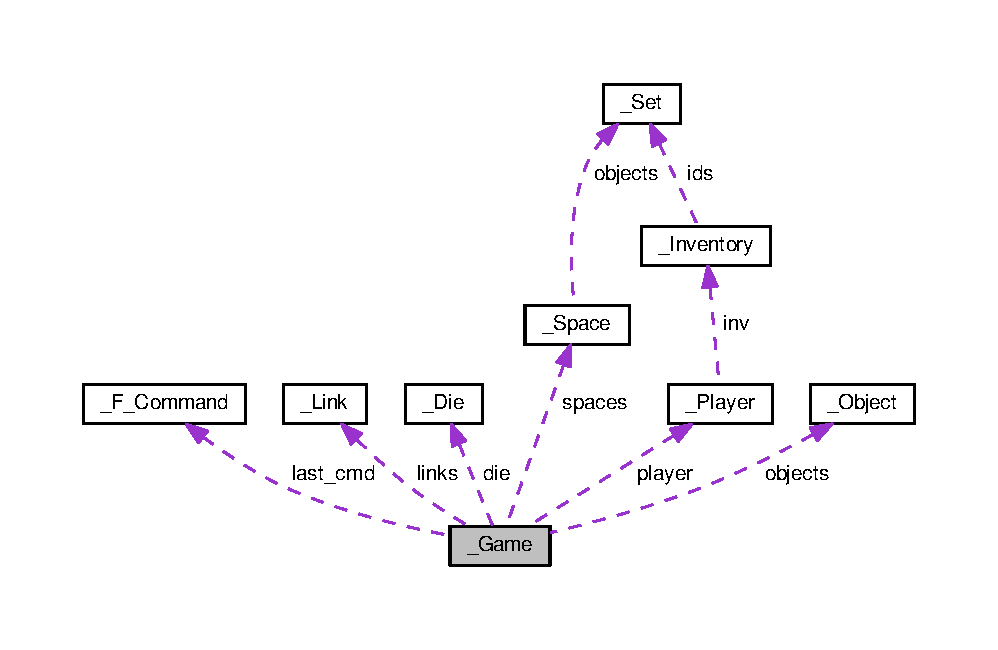
\includegraphics[width=350pt]{struct__Game__coll__graph}
\end{center}
\end{figure}
\subsection*{Public Attributes}
\begin{DoxyCompactItemize}
\item 
\hyperlink{struct__Player}{Player} $\ast$ \hyperlink{struct__Game_a31406605782d71ec00c4bf258ea76267}{player}
\item 
\hyperlink{struct__Object}{Object} $\ast$ \hyperlink{struct__Game_ad45bf5645a26e546d0060a2e61f9cf81}{objects} \mbox{[}M\+A\+X\+\_\+\+O\+B\+J\+E\+C\+TS\mbox{]}
\item 
\hyperlink{struct__Space}{Space} $\ast$ \hyperlink{struct__Game_ab4180417d9148f8abb2233ca6c4ecfe5}{spaces} \mbox{[}M\+A\+X\+\_\+\+S\+P\+A\+C\+ES+1\mbox{]}
\item 
\hyperlink{struct__Link}{Link} $\ast$ \hyperlink{struct__Game_aa4ff88aaf2a54616e5863609effad94e}{links} \mbox{[}M\+A\+X\+\_\+\+L\+I\+NK\mbox{]}
\item 
\hyperlink{die_8h_a892f0b0bf81d69a1f7a14ea238e36dd3}{Die} $\ast$ \hyperlink{struct__Game_a0d6009b5dcb080489c192a9198fa7d46}{die}
\item 
\hyperlink{struct__F__Command}{F\+\_\+\+Command} $\ast$ \hyperlink{struct__Game_a60dec64e55c5cf61b0711a11a62d18c2}{last\+\_\+cmd} \mbox{[}2\mbox{]}
\item 
\hyperlink{struct__Sprite}{Sprite} $\ast$ \hyperlink{struct__Game_a457e4328c3dfd137ba4407ad8e041cf2}{sprites} \mbox{[}M\+A\+X\+\_\+\+S\+P\+R\+I\+T\+ES\mbox{]}
\item 
\hyperlink{struct__Rule__Data}{Rule\+\_\+\+Data} $\ast$ \hyperlink{struct__Game_a2e88124c71d697f962654f2518a62109}{rule\+\_\+data}
\end{DoxyCompactItemize}


\subsection{Member Data Documentation}
\mbox{\Hypertarget{struct__Game_a0d6009b5dcb080489c192a9198fa7d46}\label{struct__Game_a0d6009b5dcb080489c192a9198fa7d46}} 
\index{\+\_\+\+Game@{\+\_\+\+Game}!die@{die}}
\index{die@{die}!\+\_\+\+Game@{\+\_\+\+Game}}
\subsubsection{\texorpdfstring{die}{die}}
{\footnotesize\ttfamily \hyperlink{die_8h_a892f0b0bf81d69a1f7a14ea238e36dd3}{Die}$\ast$ \+\_\+\+Game\+::die}

Dado \mbox{\Hypertarget{struct__Game_a60dec64e55c5cf61b0711a11a62d18c2}\label{struct__Game_a60dec64e55c5cf61b0711a11a62d18c2}} 
\index{\+\_\+\+Game@{\+\_\+\+Game}!last\+\_\+cmd@{last\+\_\+cmd}}
\index{last\+\_\+cmd@{last\+\_\+cmd}!\+\_\+\+Game@{\+\_\+\+Game}}
\subsubsection{\texorpdfstring{last\+\_\+cmd}{last\_cmd}}
{\footnotesize\ttfamily \hyperlink{struct__F__Command}{F\+\_\+\+Command}$\ast$ \+\_\+\+Game\+::last\+\_\+cmd\mbox{[}2\mbox{]}}

ultimos comandos \mbox{\Hypertarget{struct__Game_aa4ff88aaf2a54616e5863609effad94e}\label{struct__Game_aa4ff88aaf2a54616e5863609effad94e}} 
\index{\+\_\+\+Game@{\+\_\+\+Game}!links@{links}}
\index{links@{links}!\+\_\+\+Game@{\+\_\+\+Game}}
\subsubsection{\texorpdfstring{links}{links}}
{\footnotesize\ttfamily \hyperlink{struct__Link}{Link}$\ast$ \+\_\+\+Game\+::links\mbox{[}M\+A\+X\+\_\+\+L\+I\+NK\mbox{]}}

Array de links \mbox{\Hypertarget{struct__Game_ad45bf5645a26e546d0060a2e61f9cf81}\label{struct__Game_ad45bf5645a26e546d0060a2e61f9cf81}} 
\index{\+\_\+\+Game@{\+\_\+\+Game}!objects@{objects}}
\index{objects@{objects}!\+\_\+\+Game@{\+\_\+\+Game}}
\subsubsection{\texorpdfstring{objects}{objects}}
{\footnotesize\ttfamily \hyperlink{struct__Object}{Object}$\ast$ \+\_\+\+Game\+::objects\mbox{[}M\+A\+X\+\_\+\+O\+B\+J\+E\+C\+TS\mbox{]}}

Array de objetos \mbox{\Hypertarget{struct__Game_a31406605782d71ec00c4bf258ea76267}\label{struct__Game_a31406605782d71ec00c4bf258ea76267}} 
\index{\+\_\+\+Game@{\+\_\+\+Game}!player@{player}}
\index{player@{player}!\+\_\+\+Game@{\+\_\+\+Game}}
\subsubsection{\texorpdfstring{player}{player}}
{\footnotesize\ttfamily \hyperlink{struct__Player}{Player}$\ast$ \+\_\+\+Game\+::player}

Jugador \mbox{\Hypertarget{struct__Game_a2e88124c71d697f962654f2518a62109}\label{struct__Game_a2e88124c71d697f962654f2518a62109}} 
\index{\+\_\+\+Game@{\+\_\+\+Game}!rule\+\_\+data@{rule\+\_\+data}}
\index{rule\+\_\+data@{rule\+\_\+data}!\+\_\+\+Game@{\+\_\+\+Game}}
\subsubsection{\texorpdfstring{rule\+\_\+data}{rule\_data}}
{\footnotesize\ttfamily \hyperlink{struct__Rule__Data}{Rule\+\_\+\+Data}$\ast$ \+\_\+\+Game\+::rule\+\_\+data}

datos para su uso en game\+\_\+rules \mbox{\Hypertarget{struct__Game_ab4180417d9148f8abb2233ca6c4ecfe5}\label{struct__Game_ab4180417d9148f8abb2233ca6c4ecfe5}} 
\index{\+\_\+\+Game@{\+\_\+\+Game}!spaces@{spaces}}
\index{spaces@{spaces}!\+\_\+\+Game@{\+\_\+\+Game}}
\subsubsection{\texorpdfstring{spaces}{spaces}}
{\footnotesize\ttfamily \hyperlink{struct__Space}{Space}$\ast$ \+\_\+\+Game\+::spaces\mbox{[}M\+A\+X\+\_\+\+S\+P\+A\+C\+ES+1\mbox{]}}

Array de espacios \mbox{\Hypertarget{struct__Game_a457e4328c3dfd137ba4407ad8e041cf2}\label{struct__Game_a457e4328c3dfd137ba4407ad8e041cf2}} 
\index{\+\_\+\+Game@{\+\_\+\+Game}!sprites@{sprites}}
\index{sprites@{sprites}!\+\_\+\+Game@{\+\_\+\+Game}}
\subsubsection{\texorpdfstring{sprites}{sprites}}
{\footnotesize\ttfamily \hyperlink{struct__Sprite}{Sprite}$\ast$ \+\_\+\+Game\+::sprites\mbox{[}M\+A\+X\+\_\+\+S\+P\+R\+I\+T\+ES\mbox{]}}

sprites del mapa 

The documentation for this struct was generated from the following file\+:\begin{DoxyCompactItemize}
\item 
src/\hyperlink{game_8c}{game.\+c}\end{DoxyCompactItemize}

\hypertarget{struct__Graphic__engine}{}\section{\+\_\+\+Graphic\+\_\+engine Struct Reference}
\label{struct__Graphic__engine}\index{\+\_\+\+Graphic\+\_\+engine@{\+\_\+\+Graphic\+\_\+engine}}


Collaboration diagram for \+\_\+\+Graphic\+\_\+engine\+:\nopagebreak
\begin{figure}[H]
\begin{center}
\leavevmode
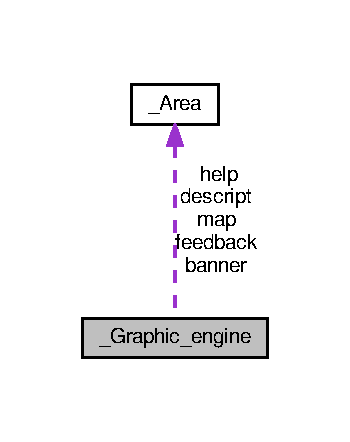
\includegraphics[width=168pt]{struct__Graphic__engine__coll__graph}
\end{center}
\end{figure}
\subsection*{Public Attributes}
\begin{DoxyCompactItemize}
\item 
\hyperlink{screen_8h_acfdfc42f6522d75fa3c16713afde8127}{Area} $\ast$ \hyperlink{struct__Graphic__engine_a1ea06bb881d335da8c31d63b3e834bdb}{map}
\item 
\hyperlink{screen_8h_acfdfc42f6522d75fa3c16713afde8127}{Area} $\ast$ \hyperlink{struct__Graphic__engine_a414bb888ecce3389c7ce348264758e58}{descript}
\item 
\hyperlink{screen_8h_acfdfc42f6522d75fa3c16713afde8127}{Area} $\ast$ \hyperlink{struct__Graphic__engine_a440dfb2c23c3c4b7d3871187371117b9}{banner}
\item 
\hyperlink{screen_8h_acfdfc42f6522d75fa3c16713afde8127}{Area} $\ast$ \hyperlink{struct__Graphic__engine_ade1d3e95ad6def427f613a4a2d101875}{help}
\item 
\hyperlink{screen_8h_acfdfc42f6522d75fa3c16713afde8127}{Area} $\ast$ \hyperlink{struct__Graphic__engine_a4fc0ef353d000b20d57fb75d898c6d2d}{feedback}
\end{DoxyCompactItemize}


\subsection{Member Data Documentation}
\index{\+\_\+\+Graphic\+\_\+engine@{\+\_\+\+Graphic\+\_\+engine}!banner@{banner}}
\index{banner@{banner}!\+\_\+\+Graphic\+\_\+engine@{\+\_\+\+Graphic\+\_\+engine}}
\subsubsection[{\texorpdfstring{banner}{banner}}]{\setlength{\rightskip}{0pt plus 5cm}{\bf Area}$\ast$ \+\_\+\+Graphic\+\_\+engine\+::banner}\hypertarget{struct__Graphic__engine_a440dfb2c23c3c4b7d3871187371117b9}{}\label{struct__Graphic__engine_a440dfb2c23c3c4b7d3871187371117b9}
banner \index{\+\_\+\+Graphic\+\_\+engine@{\+\_\+\+Graphic\+\_\+engine}!descript@{descript}}
\index{descript@{descript}!\+\_\+\+Graphic\+\_\+engine@{\+\_\+\+Graphic\+\_\+engine}}
\subsubsection[{\texorpdfstring{descript}{descript}}]{\setlength{\rightskip}{0pt plus 5cm}{\bf Area}$\ast$ \+\_\+\+Graphic\+\_\+engine\+::descript}\hypertarget{struct__Graphic__engine_a414bb888ecce3389c7ce348264758e58}{}\label{struct__Graphic__engine_a414bb888ecce3389c7ce348264758e58}
donde van las descripciones \index{\+\_\+\+Graphic\+\_\+engine@{\+\_\+\+Graphic\+\_\+engine}!feedback@{feedback}}
\index{feedback@{feedback}!\+\_\+\+Graphic\+\_\+engine@{\+\_\+\+Graphic\+\_\+engine}}
\subsubsection[{\texorpdfstring{feedback}{feedback}}]{\setlength{\rightskip}{0pt plus 5cm}{\bf Area}$\ast$ \+\_\+\+Graphic\+\_\+engine\+::feedback}\hypertarget{struct__Graphic__engine_a4fc0ef353d000b20d57fb75d898c6d2d}{}\label{struct__Graphic__engine_a4fc0ef353d000b20d57fb75d898c6d2d}
Commandos realizados e info \index{\+\_\+\+Graphic\+\_\+engine@{\+\_\+\+Graphic\+\_\+engine}!help@{help}}
\index{help@{help}!\+\_\+\+Graphic\+\_\+engine@{\+\_\+\+Graphic\+\_\+engine}}
\subsubsection[{\texorpdfstring{help}{help}}]{\setlength{\rightskip}{0pt plus 5cm}{\bf Area}$\ast$ \+\_\+\+Graphic\+\_\+engine\+::help}\hypertarget{struct__Graphic__engine_ade1d3e95ad6def427f613a4a2d101875}{}\label{struct__Graphic__engine_ade1d3e95ad6def427f613a4a2d101875}
ayuda \index{\+\_\+\+Graphic\+\_\+engine@{\+\_\+\+Graphic\+\_\+engine}!map@{map}}
\index{map@{map}!\+\_\+\+Graphic\+\_\+engine@{\+\_\+\+Graphic\+\_\+engine}}
\subsubsection[{\texorpdfstring{map}{map}}]{\setlength{\rightskip}{0pt plus 5cm}{\bf Area}$\ast$ \+\_\+\+Graphic\+\_\+engine\+::map}\hypertarget{struct__Graphic__engine_a1ea06bb881d335da8c31d63b3e834bdb}{}\label{struct__Graphic__engine_a1ea06bb881d335da8c31d63b3e834bdb}
Mapa, dibujo 

The documentation for this struct was generated from the following file\+:\begin{DoxyCompactItemize}
\item 
\hyperlink{graphic__engine_8c}{graphic\+\_\+engine.\+c}\end{DoxyCompactItemize}

\hypertarget{struct__Inventory}{}\section{\+\_\+\+Inventory Struct Reference}
\label{struct__Inventory}\index{\+\_\+\+Inventory@{\+\_\+\+Inventory}}


Collaboration diagram for \+\_\+\+Inventory\+:\nopagebreak
\begin{figure}[H]
\begin{center}
\leavevmode
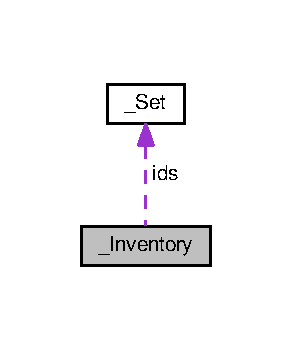
\includegraphics[width=140pt]{struct__Inventory__coll__graph}
\end{center}
\end{figure}
\subsection*{Public Attributes}
\begin{DoxyCompactItemize}
\item 
\hyperlink{set_8h_a6d3b7f7c92cbb4577ef3ef7ddbf93161}{Set} $\ast$ \hyperlink{struct__Inventory_a7f6b5d7d1111e7e8f8999c656ae27d0c}{ids}
\item 
int \hyperlink{struct__Inventory_a4b104bc26c8e030cae3032cbe7d940a3}{id\+\_\+max}
\end{DoxyCompactItemize}


\subsection{Member Data Documentation}
\index{\+\_\+\+Inventory@{\+\_\+\+Inventory}!id\+\_\+max@{id\+\_\+max}}
\index{id\+\_\+max@{id\+\_\+max}!\+\_\+\+Inventory@{\+\_\+\+Inventory}}
\subsubsection[{\texorpdfstring{id\+\_\+max}{id_max}}]{\setlength{\rightskip}{0pt plus 5cm}int \+\_\+\+Inventory\+::id\+\_\+max}\hypertarget{struct__Inventory_a4b104bc26c8e030cae3032cbe7d940a3}{}\label{struct__Inventory_a4b104bc26c8e030cae3032cbe7d940a3}
Maximo de lugares \index{\+\_\+\+Inventory@{\+\_\+\+Inventory}!ids@{ids}}
\index{ids@{ids}!\+\_\+\+Inventory@{\+\_\+\+Inventory}}
\subsubsection[{\texorpdfstring{ids}{ids}}]{\setlength{\rightskip}{0pt plus 5cm}{\bf Set}$\ast$ \+\_\+\+Inventory\+::ids}\hypertarget{struct__Inventory_a7f6b5d7d1111e7e8f8999c656ae27d0c}{}\label{struct__Inventory_a7f6b5d7d1111e7e8f8999c656ae27d0c}
Inventario 

The documentation for this struct was generated from the following file\+:\begin{DoxyCompactItemize}
\item 
\hyperlink{inventory_8c}{inventory.\+c}\end{DoxyCompactItemize}

\hypertarget{struct__Link}{}\section{\+\_\+\+Link Struct Reference}
\label{struct__Link}\index{\+\_\+\+Link@{\+\_\+\+Link}}
\subsection*{Public Attributes}
\begin{DoxyCompactItemize}
\item 
\hyperlink{types_8h_a845e604fb28f7e3d97549da3448149d3}{Id} \hyperlink{struct__Link_a3c2eb94d5f272bf373c113a868e3d367}{link\+Id}
\item 
\hyperlink{types_8h_a845e604fb28f7e3d97549da3448149d3}{Id} \hyperlink{struct__Link_a851b2cb675c25aaa73ebbaa58b8db1a2}{linkspace1}
\item 
\hyperlink{types_8h_a845e604fb28f7e3d97549da3448149d3}{Id} \hyperlink{struct__Link_aac79e76abc5512cd08a381eb835d59f0}{linkspace2}
\item 
int \hyperlink{struct__Link_a112e92df8f8eae3055ab45793ed4a660}{direction}
\item 
\hyperlink{types_8h_aa60f669816b146d6373c62d9625e52ad}{Link\+Status} \hyperlink{struct__Link_ab4d6f65f126e9a41440828d2317b7a79}{door}
\end{DoxyCompactItemize}


\subsection{Member Data Documentation}
\index{\+\_\+\+Link@{\+\_\+\+Link}!direction@{direction}}
\index{direction@{direction}!\+\_\+\+Link@{\+\_\+\+Link}}
\subsubsection[{\texorpdfstring{direction}{direction}}]{\setlength{\rightskip}{0pt plus 5cm}int \+\_\+\+Link\+::direction}\hypertarget{struct__Link_a112e92df8f8eae3055ab45793ed4a660}{}\label{struct__Link_a112e92df8f8eae3055ab45793ed4a660}
Norte, sur, este u oeste \index{\+\_\+\+Link@{\+\_\+\+Link}!door@{door}}
\index{door@{door}!\+\_\+\+Link@{\+\_\+\+Link}}
\subsubsection[{\texorpdfstring{door}{door}}]{\setlength{\rightskip}{0pt plus 5cm}{\bf Link\+Status} \+\_\+\+Link\+::door}\hypertarget{struct__Link_ab4d6f65f126e9a41440828d2317b7a79}{}\label{struct__Link_ab4d6f65f126e9a41440828d2317b7a79}
Estatus del link O\+P\+E\+N\+E\+D/\+C\+L\+O\+S\+ED \index{\+\_\+\+Link@{\+\_\+\+Link}!link\+Id@{link\+Id}}
\index{link\+Id@{link\+Id}!\+\_\+\+Link@{\+\_\+\+Link}}
\subsubsection[{\texorpdfstring{link\+Id}{linkId}}]{\setlength{\rightskip}{0pt plus 5cm}{\bf Id} \+\_\+\+Link\+::link\+Id}\hypertarget{struct__Link_a3c2eb94d5f272bf373c113a868e3d367}{}\label{struct__Link_a3c2eb94d5f272bf373c113a868e3d367}
Id del link \index{\+\_\+\+Link@{\+\_\+\+Link}!linkspace1@{linkspace1}}
\index{linkspace1@{linkspace1}!\+\_\+\+Link@{\+\_\+\+Link}}
\subsubsection[{\texorpdfstring{linkspace1}{linkspace1}}]{\setlength{\rightskip}{0pt plus 5cm}{\bf Id} \+\_\+\+Link\+::linkspace1}\hypertarget{struct__Link_a851b2cb675c25aaa73ebbaa58b8db1a2}{}\label{struct__Link_a851b2cb675c25aaa73ebbaa58b8db1a2}
\index{\+\_\+\+Link@{\+\_\+\+Link}!linkspace2@{linkspace2}}
\index{linkspace2@{linkspace2}!\+\_\+\+Link@{\+\_\+\+Link}}
\subsubsection[{\texorpdfstring{linkspace2}{linkspace2}}]{\setlength{\rightskip}{0pt plus 5cm}{\bf Id} \+\_\+\+Link\+::linkspace2}\hypertarget{struct__Link_aac79e76abc5512cd08a381eb835d59f0}{}\label{struct__Link_aac79e76abc5512cd08a381eb835d59f0}
id de los espacios conectados 

The documentation for this struct was generated from the following file\+:\begin{DoxyCompactItemize}
\item 
\hyperlink{link_8c}{link.\+c}\end{DoxyCompactItemize}

\hypertarget{struct__Object}{\section{\+\_\+\+Object Struct Reference}
\label{struct__Object}\index{\+\_\+\+Object@{\+\_\+\+Object}}
}
\subsection*{Public Attributes}
\begin{DoxyCompactItemize}
\item 
char \hyperlink{struct__Object_a5f13167436f75d12f48d3f152ce91d0a}{name} \mbox{[}\hyperlink{types_8h_a431b1676533a0e1714aff7d6a5542406}{S\+T\+D\+S\+I\+Z\+E}\mbox{]}
\item 
char \hyperlink{struct__Object_a4797c28bbea5a64792ec85433ee7215e}{description} \mbox{[}\hyperlink{types_8h_a431b1676533a0e1714aff7d6a5542406}{S\+T\+D\+S\+I\+Z\+E}\mbox{]}
\item 
\hyperlink{types_8h_a845e604fb28f7e3d97549da3448149d3}{Id} \hyperlink{struct__Object_a3cff7a0e8dc4e9d23895ed9af1b7653a}{id}
\end{DoxyCompactItemize}


\subsection{Member Data Documentation}
\hypertarget{struct__Object_a4797c28bbea5a64792ec85433ee7215e}{\index{\+\_\+\+Object@{\+\_\+\+Object}!description@{description}}
\index{description@{description}!\+\_\+\+Object@{\+\_\+\+Object}}
\subsubsection[{description}]{\setlength{\rightskip}{0pt plus 5cm}char \+\_\+\+Object\+::description\mbox{[}{\bf S\+T\+D\+S\+I\+Z\+E}\mbox{]}}}\label{struct__Object_a4797c28bbea5a64792ec85433ee7215e}
Descripcion del objeto \hypertarget{struct__Object_a3cff7a0e8dc4e9d23895ed9af1b7653a}{\index{\+\_\+\+Object@{\+\_\+\+Object}!id@{id}}
\index{id@{id}!\+\_\+\+Object@{\+\_\+\+Object}}
\subsubsection[{id}]{\setlength{\rightskip}{0pt plus 5cm}{\bf Id} \+\_\+\+Object\+::id}}\label{struct__Object_a3cff7a0e8dc4e9d23895ed9af1b7653a}
Identificador \hypertarget{struct__Object_a5f13167436f75d12f48d3f152ce91d0a}{\index{\+\_\+\+Object@{\+\_\+\+Object}!name@{name}}
\index{name@{name}!\+\_\+\+Object@{\+\_\+\+Object}}
\subsubsection[{name}]{\setlength{\rightskip}{0pt plus 5cm}char \+\_\+\+Object\+::name\mbox{[}{\bf S\+T\+D\+S\+I\+Z\+E}\mbox{]}}}\label{struct__Object_a5f13167436f75d12f48d3f152ce91d0a}
Nombre del objeto 

The documentation for this struct was generated from the following file\+:\begin{DoxyCompactItemize}
\item 
\hyperlink{object_8c}{object.\+c}\end{DoxyCompactItemize}

\hypertarget{struct__Player}{}\section{\+\_\+\+Player Struct Reference}
\label{struct__Player}\index{\+\_\+\+Player@{\+\_\+\+Player}}


Collaboration diagram for \+\_\+\+Player\+:\nopagebreak
\begin{figure}[H]
\begin{center}
\leavevmode
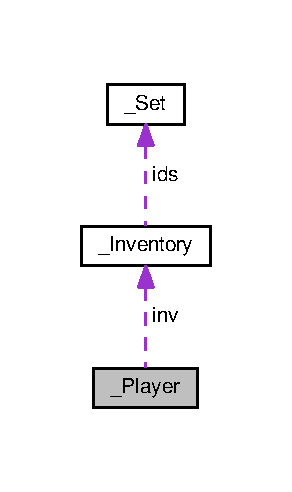
\includegraphics[width=140pt]{struct__Player__coll__graph}
\end{center}
\end{figure}
\subsection*{Public Attributes}
\begin{DoxyCompactItemize}
\item 
char \hyperlink{struct__Player_abd3fbad9568ff1e608654d58e71b8c58}{name} \mbox{[}\hyperlink{types_8h_a431b1676533a0e1714aff7d6a5542406}{S\+T\+D\+S\+I\+ZE}\mbox{]}
\item 
\hyperlink{types_8h_a845e604fb28f7e3d97549da3448149d3}{Id} \hyperlink{struct__Player_aca2cb83e7a18dea36c33ad94e36a1e54}{location\+\_\+id}
\item 
\hyperlink{inventory_8h_a2253bf64ac4ce6a9c1d6f39c0b0d32a3}{Inventory} $\ast$ \hyperlink{struct__Player_aaaeeb03326c37ce62c333c2b94fde23c}{inv}
\item 
\hyperlink{types_8h_a845e604fb28f7e3d97549da3448149d3}{Id} \hyperlink{struct__Player_a60d635cd063816a9c1bd873f4868bb90}{id}
\end{DoxyCompactItemize}


\subsection{Member Data Documentation}
\index{\+\_\+\+Player@{\+\_\+\+Player}!id@{id}}
\index{id@{id}!\+\_\+\+Player@{\+\_\+\+Player}}
\subsubsection[{\texorpdfstring{id}{id}}]{\setlength{\rightskip}{0pt plus 5cm}{\bf Id} \+\_\+\+Player\+::id}\hypertarget{struct__Player_a60d635cd063816a9c1bd873f4868bb90}{}\label{struct__Player_a60d635cd063816a9c1bd873f4868bb90}
id del jugador \index{\+\_\+\+Player@{\+\_\+\+Player}!inv@{inv}}
\index{inv@{inv}!\+\_\+\+Player@{\+\_\+\+Player}}
\subsubsection[{\texorpdfstring{inv}{inv}}]{\setlength{\rightskip}{0pt plus 5cm}{\bf Inventory}$\ast$ \+\_\+\+Player\+::inv}\hypertarget{struct__Player_aaaeeb03326c37ce62c333c2b94fde23c}{}\label{struct__Player_aaaeeb03326c37ce62c333c2b94fde23c}
inventario del jugador \index{\+\_\+\+Player@{\+\_\+\+Player}!location\+\_\+id@{location\+\_\+id}}
\index{location\+\_\+id@{location\+\_\+id}!\+\_\+\+Player@{\+\_\+\+Player}}
\subsubsection[{\texorpdfstring{location\+\_\+id}{location_id}}]{\setlength{\rightskip}{0pt plus 5cm}{\bf Id} \+\_\+\+Player\+::location\+\_\+id}\hypertarget{struct__Player_aca2cb83e7a18dea36c33ad94e36a1e54}{}\label{struct__Player_aca2cb83e7a18dea36c33ad94e36a1e54}
id de donde esta \index{\+\_\+\+Player@{\+\_\+\+Player}!name@{name}}
\index{name@{name}!\+\_\+\+Player@{\+\_\+\+Player}}
\subsubsection[{\texorpdfstring{name}{name}}]{\setlength{\rightskip}{0pt plus 5cm}char \+\_\+\+Player\+::name\mbox{[}{\bf S\+T\+D\+S\+I\+ZE}\mbox{]}}\hypertarget{struct__Player_abd3fbad9568ff1e608654d58e71b8c58}{}\label{struct__Player_abd3fbad9568ff1e608654d58e71b8c58}
Nombre del jugador 

The documentation for this struct was generated from the following file\+:\begin{DoxyCompactItemize}
\item 
\hyperlink{player_8c}{player.\+c}\end{DoxyCompactItemize}

\hypertarget{struct__Set}{}\section{\+\_\+\+Set Struct Reference}
\label{struct__Set}\index{\+\_\+\+Set@{\+\_\+\+Set}}
\subsection*{Public Attributes}
\begin{DoxyCompactItemize}
\item 
Id \hyperlink{struct__Set_adde563bd36bf2d00bd5a49b493c4f3bb}{id\+\_\+list} \mbox{[}M\+A\+X\+\_\+\+I\+N\+V\+\_\+\+S\+I\+ZE\mbox{]}
\item 
int \hyperlink{struct__Set_afe941cf156f1000d962bff58835ba853}{id\+\_\+total}
\end{DoxyCompactItemize}


\subsection{Member Data Documentation}
\mbox{\Hypertarget{struct__Set_adde563bd36bf2d00bd5a49b493c4f3bb}\label{struct__Set_adde563bd36bf2d00bd5a49b493c4f3bb}} 
\index{\+\_\+\+Set@{\+\_\+\+Set}!id\+\_\+list@{id\+\_\+list}}
\index{id\+\_\+list@{id\+\_\+list}!\+\_\+\+Set@{\+\_\+\+Set}}
\subsubsection{\texorpdfstring{id\+\_\+list}{id\_list}}
{\footnotesize\ttfamily Id \+\_\+\+Set\+::id\+\_\+list\mbox{[}M\+A\+X\+\_\+\+I\+N\+V\+\_\+\+S\+I\+ZE\mbox{]}}

Array \mbox{\Hypertarget{struct__Set_afe941cf156f1000d962bff58835ba853}\label{struct__Set_afe941cf156f1000d962bff58835ba853}} 
\index{\+\_\+\+Set@{\+\_\+\+Set}!id\+\_\+total@{id\+\_\+total}}
\index{id\+\_\+total@{id\+\_\+total}!\+\_\+\+Set@{\+\_\+\+Set}}
\subsubsection{\texorpdfstring{id\+\_\+total}{id\_total}}
{\footnotesize\ttfamily int \+\_\+\+Set\+::id\+\_\+total}

Total del array 

The documentation for this struct was generated from the following file\+:\begin{DoxyCompactItemize}
\item 
src/\hyperlink{set_8c}{set.\+c}\end{DoxyCompactItemize}

\hypertarget{struct__Space}{}\section{\+\_\+\+Space Struct Reference}
\label{struct__Space}\index{\+\_\+\+Space@{\+\_\+\+Space}}


Collaboration diagram for \+\_\+\+Space\+:
% FIG 0
\subsection*{Public Attributes}
\begin{DoxyCompactItemize}
\item 
\hyperlink{types_8h_a845e604fb28f7e3d97549da3448149d3}{Id} \hyperlink{struct__Space_a70cb461deb9ac073e401b607339b567f}{id}
\item 
char \hyperlink{struct__Space_a4e8775f2ba9ae19392f9942dbb5f5ec0}{name} \mbox{[}\hyperlink{types_8h_a92ed8507d1cd2331ad09275c5c4c1c89}{W\+O\+R\+D\+\_\+\+S\+I\+ZE}\mbox{]}
\item 
char \hyperlink{struct__Space_a2a50aacb78d1d0f65f5b14f94ed81d80}{description} \mbox{[}\hyperlink{types_8h_a92ed8507d1cd2331ad09275c5c4c1c89}{W\+O\+R\+D\+\_\+\+S\+I\+ZE}\mbox{]}
\item 
\hyperlink{types_8h_a845e604fb28f7e3d97549da3448149d3}{Id} \hyperlink{struct__Space_a3f2998ecc940b5cdab73e38188886902}{link\+North}
\item 
\hyperlink{types_8h_a845e604fb28f7e3d97549da3448149d3}{Id} \hyperlink{struct__Space_a642c37093a6ccc0203a655c3fc0a93d3}{link\+South}
\item 
\hyperlink{types_8h_a845e604fb28f7e3d97549da3448149d3}{Id} \hyperlink{struct__Space_adbf9d4d57d188ef48d3e361fb77a92cf}{link\+East}
\item 
\hyperlink{types_8h_a845e604fb28f7e3d97549da3448149d3}{Id} \hyperlink{struct__Space_aaa6f5fa10a67afc466e3b272099dc398}{link\+West}
\item 
char \hyperlink{struct__Space_a0a71c4c0a4a1698f7d860ba5b80beb7f}{gdesc} \mbox{[}3\mbox{]}\mbox{[}21\mbox{]}
\item 
\hyperlink{set_8h_a6d3b7f7c92cbb4577ef3ef7ddbf93161}{Set} $\ast$ \hyperlink{struct__Space_a661ed8b0fc8085b6db70188aa5085625}{objects}
\end{DoxyCompactItemize}


\subsection{Member Data Documentation}
\index{\+\_\+\+Space@{\+\_\+\+Space}!description@{description}}
\index{description@{description}!\+\_\+\+Space@{\+\_\+\+Space}}
\subsubsection[{\texorpdfstring{description}{description}}]{\setlength{\rightskip}{0pt plus 5cm}char \+\_\+\+Space\+::description\mbox{[}{\bf W\+O\+R\+D\+\_\+\+S\+I\+ZE}\mbox{]}}\hypertarget{struct__Space_a2a50aacb78d1d0f65f5b14f94ed81d80}{}\label{struct__Space_a2a50aacb78d1d0f65f5b14f94ed81d80}
\index{\+\_\+\+Space@{\+\_\+\+Space}!gdesc@{gdesc}}
\index{gdesc@{gdesc}!\+\_\+\+Space@{\+\_\+\+Space}}
\subsubsection[{\texorpdfstring{gdesc}{gdesc}}]{\setlength{\rightskip}{0pt plus 5cm}char \+\_\+\+Space\+::gdesc\mbox{[}3\mbox{]}\mbox{[}21\mbox{]}}\hypertarget{struct__Space_a0a71c4c0a4a1698f7d860ba5b80beb7f}{}\label{struct__Space_a0a71c4c0a4a1698f7d860ba5b80beb7f}
\index{\+\_\+\+Space@{\+\_\+\+Space}!id@{id}}
\index{id@{id}!\+\_\+\+Space@{\+\_\+\+Space}}
\subsubsection[{\texorpdfstring{id}{id}}]{\setlength{\rightskip}{0pt plus 5cm}{\bf Id} \+\_\+\+Space\+::id}\hypertarget{struct__Space_a70cb461deb9ac073e401b607339b567f}{}\label{struct__Space_a70cb461deb9ac073e401b607339b567f}
\index{\+\_\+\+Space@{\+\_\+\+Space}!link\+East@{link\+East}}
\index{link\+East@{link\+East}!\+\_\+\+Space@{\+\_\+\+Space}}
\subsubsection[{\texorpdfstring{link\+East}{linkEast}}]{\setlength{\rightskip}{0pt plus 5cm}{\bf Id} \+\_\+\+Space\+::link\+East}\hypertarget{struct__Space_adbf9d4d57d188ef48d3e361fb77a92cf}{}\label{struct__Space_adbf9d4d57d188ef48d3e361fb77a92cf}
\index{\+\_\+\+Space@{\+\_\+\+Space}!link\+North@{link\+North}}
\index{link\+North@{link\+North}!\+\_\+\+Space@{\+\_\+\+Space}}
\subsubsection[{\texorpdfstring{link\+North}{linkNorth}}]{\setlength{\rightskip}{0pt plus 5cm}{\bf Id} \+\_\+\+Space\+::link\+North}\hypertarget{struct__Space_a3f2998ecc940b5cdab73e38188886902}{}\label{struct__Space_a3f2998ecc940b5cdab73e38188886902}
\index{\+\_\+\+Space@{\+\_\+\+Space}!link\+South@{link\+South}}
\index{link\+South@{link\+South}!\+\_\+\+Space@{\+\_\+\+Space}}
\subsubsection[{\texorpdfstring{link\+South}{linkSouth}}]{\setlength{\rightskip}{0pt plus 5cm}{\bf Id} \+\_\+\+Space\+::link\+South}\hypertarget{struct__Space_a642c37093a6ccc0203a655c3fc0a93d3}{}\label{struct__Space_a642c37093a6ccc0203a655c3fc0a93d3}
\index{\+\_\+\+Space@{\+\_\+\+Space}!link\+West@{link\+West}}
\index{link\+West@{link\+West}!\+\_\+\+Space@{\+\_\+\+Space}}
\subsubsection[{\texorpdfstring{link\+West}{linkWest}}]{\setlength{\rightskip}{0pt plus 5cm}{\bf Id} \+\_\+\+Space\+::link\+West}\hypertarget{struct__Space_aaa6f5fa10a67afc466e3b272099dc398}{}\label{struct__Space_aaa6f5fa10a67afc466e3b272099dc398}
\index{\+\_\+\+Space@{\+\_\+\+Space}!name@{name}}
\index{name@{name}!\+\_\+\+Space@{\+\_\+\+Space}}
\subsubsection[{\texorpdfstring{name}{name}}]{\setlength{\rightskip}{0pt plus 5cm}char \+\_\+\+Space\+::name\mbox{[}{\bf W\+O\+R\+D\+\_\+\+S\+I\+ZE}\mbox{]}}\hypertarget{struct__Space_a4e8775f2ba9ae19392f9942dbb5f5ec0}{}\label{struct__Space_a4e8775f2ba9ae19392f9942dbb5f5ec0}
\index{\+\_\+\+Space@{\+\_\+\+Space}!objects@{objects}}
\index{objects@{objects}!\+\_\+\+Space@{\+\_\+\+Space}}
\subsubsection[{\texorpdfstring{objects}{objects}}]{\setlength{\rightskip}{0pt plus 5cm}{\bf Set}$\ast$ \+\_\+\+Space\+::objects}\hypertarget{struct__Space_a661ed8b0fc8085b6db70188aa5085625}{}\label{struct__Space_a661ed8b0fc8085b6db70188aa5085625}


The documentation for this struct was generated from the following file\+:\begin{DoxyCompactItemize}
\item 
\hyperlink{space_8c}{space.\+c}\end{DoxyCompactItemize}

\hypertarget{struct__Sprite}{}\section{\+\_\+\+Sprite Struct Reference}
\label{struct__Sprite}\index{\+\_\+\+Sprite@{\+\_\+\+Sprite}}
\subsection*{Public Attributes}
\begin{DoxyCompactItemize}
\item 
Id \hyperlink{struct__Sprite_ade53af91be4735711bed7748f69fbc2a}{id}
\item 
char \hyperlink{struct__Sprite_add6396519e5c35e3e0d04d8519d5e6c2}{data} \mbox{[}17\mbox{]}\mbox{[}39\mbox{]}
\end{DoxyCompactItemize}


\subsection{Member Data Documentation}
\mbox{\Hypertarget{struct__Sprite_add6396519e5c35e3e0d04d8519d5e6c2}\label{struct__Sprite_add6396519e5c35e3e0d04d8519d5e6c2}} 
\index{\+\_\+\+Sprite@{\+\_\+\+Sprite}!data@{data}}
\index{data@{data}!\+\_\+\+Sprite@{\+\_\+\+Sprite}}
\subsubsection{\texorpdfstring{data}{data}}
{\footnotesize\ttfamily char \+\_\+\+Sprite\+::data\mbox{[}17\mbox{]}\mbox{[}39\mbox{]}}

Datos en ascii \mbox{\Hypertarget{struct__Sprite_ade53af91be4735711bed7748f69fbc2a}\label{struct__Sprite_ade53af91be4735711bed7748f69fbc2a}} 
\index{\+\_\+\+Sprite@{\+\_\+\+Sprite}!id@{id}}
\index{id@{id}!\+\_\+\+Sprite@{\+\_\+\+Sprite}}
\subsubsection{\texorpdfstring{id}{id}}
{\footnotesize\ttfamily Id \+\_\+\+Sprite\+::id}

Id del sprite 

The documentation for this struct was generated from the following file\+:\begin{DoxyCompactItemize}
\item 
src/\hyperlink{sprite_8c}{sprite.\+c}\end{DoxyCompactItemize}

\chapter{File Documentation}
\hypertarget{command_8c}{}\section{command.\+c File Reference}
\label{command_8c}\index{command.\+c@{command.\+c}}


Commands and user input.  


{\ttfamily \#include $<$stdio.\+h$>$}\\*
{\ttfamily \#include $<$strings.\+h$>$}\\*
{\ttfamily \#include \char`\"{}../include/command.\+h\char`\"{}}\\*
Include dependency graph for command.\+c\+:\nopagebreak
\begin{figure}[H]
\begin{center}
\leavevmode
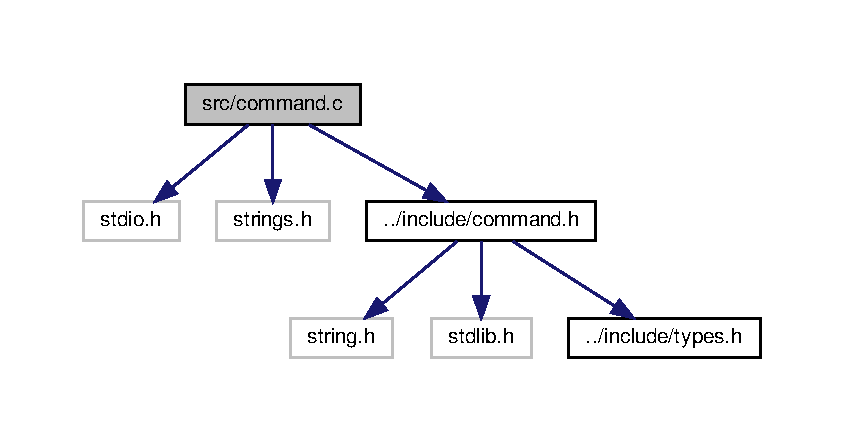
\includegraphics[width=350pt]{command_8c__incl}
\end{center}
\end{figure}
\subsection*{Classes}
\begin{DoxyCompactItemize}
\item 
struct \hyperlink{struct__F__Command}{\+\_\+\+F\+\_\+\+Command}
\end{DoxyCompactItemize}
\subsection*{Macros}
\begin{DoxyCompactItemize}
\item 
\#define \hyperlink{command_8c_a2b1bd24d2eddf8081d8c541e4cc4fd4b}{C\+M\+D\+\_\+\+L\+E\+N\+G\+HT}~30
\item 
\#define \hyperlink{command_8c_ae180fe89f0ae48ce5c80ffaa18de9271}{N\+\_\+\+C\+MD}~11
\end{DoxyCompactItemize}
\subsection*{Functions}
\begin{DoxyCompactItemize}
\item 
\hyperlink{types_8h_a32c27cc471df37f4fc818d65de0a56c4}{S\+T\+A\+T\+US} \hyperlink{command_8c_a08a814029449fcbfd410755cafd2e275}{get\+\_\+user\+\_\+input} (\hyperlink{command_8h_a76085817cb558dc3640088040ba47898}{F\+\_\+\+Command} $\ast$command)
\item 
\hyperlink{command_8h_a76085817cb558dc3640088040ba47898}{F\+\_\+\+Command} $\ast$ \hyperlink{command_8c_ae66916e90ab149b0bb6222b1ce60f09b}{command\+\_\+create} ()
\item 
\hyperlink{types_8h_a32c27cc471df37f4fc818d65de0a56c4}{S\+T\+A\+T\+US} \hyperlink{command_8c_a0f65c3e80483261e7a4212ec1686c209}{command\+\_\+set\+Cmd} (\hyperlink{command_8h_a76085817cb558dc3640088040ba47898}{F\+\_\+\+Command} $\ast$cmd, \hyperlink{command_8h_a0473597db8c45c0289b6b8e2f8abbe32}{T\+\_\+\+Command} command)
\item 
\hyperlink{command_8h_a0473597db8c45c0289b6b8e2f8abbe32}{T\+\_\+\+Command} \hyperlink{command_8c_a2438443fd32ff9ba62670005fde274b6}{command\+\_\+get\+Cmd} (\hyperlink{command_8h_a76085817cb558dc3640088040ba47898}{F\+\_\+\+Command} $\ast$cmd)
\item 
char $\ast$ \hyperlink{command_8c_abfe79582caad3f5d3042ebaddf62e03c}{command\+\_\+get\+\_\+id} (\hyperlink{command_8h_a76085817cb558dc3640088040ba47898}{F\+\_\+\+Command} $\ast$cmd)
\item 
\hyperlink{types_8h_a32c27cc471df37f4fc818d65de0a56c4}{S\+T\+A\+T\+US} \hyperlink{command_8c_ae36f03b1858db756583a061b49d86f0c}{command\+\_\+set\+\_\+id} (\hyperlink{command_8h_a76085817cb558dc3640088040ba47898}{F\+\_\+\+Command} $\ast$cmd, char $\ast$string)
\item 
void \hyperlink{command_8c_a7717a3f0b1aae92678c1fec154019d22}{command\+\_\+free} (\hyperlink{command_8h_a76085817cb558dc3640088040ba47898}{F\+\_\+\+Command} $\ast$cmd)
\end{DoxyCompactItemize}
\subsection*{Variables}
\begin{DoxyCompactItemize}
\item 
char $\ast$ \hyperlink{command_8c_aa491d83d4e2f55a3074e418318a8d0fe}{cmd\+\_\+to\+\_\+str} \mbox{[}\hyperlink{command_8c_ae180fe89f0ae48ce5c80ffaa18de9271}{N\+\_\+\+C\+MD}\mbox{]} = \{\char`\"{}No command\char`\"{}, \char`\"{}Unknown\char`\"{}, \char`\"{}Exit\char`\"{}, \char`\"{}Pickup\char`\"{}, \char`\"{}Drop\char`\"{}, \char`\"{}Roll\char`\"{}, \char`\"{}Move\char`\"{}, \char`\"{}Check\char`\"{}, \char`\"{}Turnon\char`\"{}, \char`\"{}Turnoff\char`\"{}, \char`\"{}Open\char`\"{}\}
\item 
char $\ast$ \hyperlink{command_8c_a6397d54c2691d7e8ffe9a8da5db5df58}{short\+\_\+cmd\+\_\+to\+\_\+str} \mbox{[}\hyperlink{command_8c_ae180fe89f0ae48ce5c80ffaa18de9271}{N\+\_\+\+C\+MD}\mbox{]} = \{\char`\"{}\char`\"{}, \char`\"{}\char`\"{}, \char`\"{}e\char`\"{}, \char`\"{}p\char`\"{}, \char`\"{}d\char`\"{}, \char`\"{}r\char`\"{}, \char`\"{}m\char`\"{}, \char`\"{}c\char`\"{}, \char`\"{}to\char`\"{}, \char`\"{}tf\char`\"{}, \char`\"{}o\char`\"{}\}
\end{DoxyCompactItemize}


\subsection{Detailed Description}
Commands and user input. 

Defines functions for space manipulation.

\begin{DoxyAuthor}{Author}
Antonio Solana 
\end{DoxyAuthor}
\begin{DoxyCopyright}{Copyright}
G\+NU Public License
\end{DoxyCopyright}
\begin{DoxyAuthor}{Author}
Catal�n Rotaru 
\end{DoxyAuthor}
\begin{DoxyCopyright}{Copyright}
G\+NU Public License 
\end{DoxyCopyright}


\subsection{Macro Definition Documentation}
\index{command.\+c@{command.\+c}!C\+M\+D\+\_\+\+L\+E\+N\+G\+HT@{C\+M\+D\+\_\+\+L\+E\+N\+G\+HT}}
\index{C\+M\+D\+\_\+\+L\+E\+N\+G\+HT@{C\+M\+D\+\_\+\+L\+E\+N\+G\+HT}!command.\+c@{command.\+c}}
\subsubsection[{\texorpdfstring{C\+M\+D\+\_\+\+L\+E\+N\+G\+HT}{CMD_LENGHT}}]{\setlength{\rightskip}{0pt plus 5cm}\#define C\+M\+D\+\_\+\+L\+E\+N\+G\+HT~30}\hypertarget{command_8c_a2b1bd24d2eddf8081d8c541e4cc4fd4b}{}\label{command_8c_a2b1bd24d2eddf8081d8c541e4cc4fd4b}
\index{command.\+c@{command.\+c}!N\+\_\+\+C\+MD@{N\+\_\+\+C\+MD}}
\index{N\+\_\+\+C\+MD@{N\+\_\+\+C\+MD}!command.\+c@{command.\+c}}
\subsubsection[{\texorpdfstring{N\+\_\+\+C\+MD}{N_CMD}}]{\setlength{\rightskip}{0pt plus 5cm}\#define N\+\_\+\+C\+MD~11}\hypertarget{command_8c_ae180fe89f0ae48ce5c80ffaa18de9271}{}\label{command_8c_ae180fe89f0ae48ce5c80ffaa18de9271}


\subsection{Function Documentation}
\index{command.\+c@{command.\+c}!command\+\_\+create@{command\+\_\+create}}
\index{command\+\_\+create@{command\+\_\+create}!command.\+c@{command.\+c}}
\subsubsection[{\texorpdfstring{command\+\_\+create()}{command_create()}}]{\setlength{\rightskip}{0pt plus 5cm}{\bf F\+\_\+\+Command}$\ast$ command\+\_\+create (
\begin{DoxyParamCaption}
{}
\end{DoxyParamCaption}
)}\hypertarget{command_8c_ae66916e90ab149b0bb6222b1ce60f09b}{}\label{command_8c_ae66916e90ab149b0bb6222b1ce60f09b}
\index{command.\+c@{command.\+c}!command\+\_\+free@{command\+\_\+free}}
\index{command\+\_\+free@{command\+\_\+free}!command.\+c@{command.\+c}}
\subsubsection[{\texorpdfstring{command\+\_\+free(\+F\+\_\+\+Command $\ast$cmd)}{command_free(F_Command *cmd)}}]{\setlength{\rightskip}{0pt plus 5cm}void command\+\_\+free (
\begin{DoxyParamCaption}
\item[{{\bf F\+\_\+\+Command} $\ast$}]{cmd}
\end{DoxyParamCaption}
)}\hypertarget{command_8c_a7717a3f0b1aae92678c1fec154019d22}{}\label{command_8c_a7717a3f0b1aae92678c1fec154019d22}
\index{command.\+c@{command.\+c}!command\+\_\+get\+\_\+id@{command\+\_\+get\+\_\+id}}
\index{command\+\_\+get\+\_\+id@{command\+\_\+get\+\_\+id}!command.\+c@{command.\+c}}
\subsubsection[{\texorpdfstring{command\+\_\+get\+\_\+id(\+F\+\_\+\+Command $\ast$cmd)}{command_get_id(F_Command *cmd)}}]{\setlength{\rightskip}{0pt plus 5cm}char$\ast$ command\+\_\+get\+\_\+id (
\begin{DoxyParamCaption}
\item[{{\bf F\+\_\+\+Command} $\ast$}]{cmd}
\end{DoxyParamCaption}
)}\hypertarget{command_8c_abfe79582caad3f5d3042ebaddf62e03c}{}\label{command_8c_abfe79582caad3f5d3042ebaddf62e03c}
\index{command.\+c@{command.\+c}!command\+\_\+get\+Cmd@{command\+\_\+get\+Cmd}}
\index{command\+\_\+get\+Cmd@{command\+\_\+get\+Cmd}!command.\+c@{command.\+c}}
\subsubsection[{\texorpdfstring{command\+\_\+get\+Cmd(\+F\+\_\+\+Command $\ast$cmd)}{command_getCmd(F_Command *cmd)}}]{\setlength{\rightskip}{0pt plus 5cm}{\bf T\+\_\+\+Command} command\+\_\+get\+Cmd (
\begin{DoxyParamCaption}
\item[{{\bf F\+\_\+\+Command} $\ast$}]{cmd}
\end{DoxyParamCaption}
)}\hypertarget{command_8c_a2438443fd32ff9ba62670005fde274b6}{}\label{command_8c_a2438443fd32ff9ba62670005fde274b6}
\index{command.\+c@{command.\+c}!command\+\_\+set\+\_\+id@{command\+\_\+set\+\_\+id}}
\index{command\+\_\+set\+\_\+id@{command\+\_\+set\+\_\+id}!command.\+c@{command.\+c}}
\subsubsection[{\texorpdfstring{command\+\_\+set\+\_\+id(\+F\+\_\+\+Command $\ast$cmd, char $\ast$string)}{command_set_id(F_Command *cmd, char *string)}}]{\setlength{\rightskip}{0pt plus 5cm}{\bf S\+T\+A\+T\+US} command\+\_\+set\+\_\+id (
\begin{DoxyParamCaption}
\item[{{\bf F\+\_\+\+Command} $\ast$}]{cmd, }
\item[{char $\ast$}]{string}
\end{DoxyParamCaption}
)}\hypertarget{command_8c_ae36f03b1858db756583a061b49d86f0c}{}\label{command_8c_ae36f03b1858db756583a061b49d86f0c}
\index{command.\+c@{command.\+c}!command\+\_\+set\+Cmd@{command\+\_\+set\+Cmd}}
\index{command\+\_\+set\+Cmd@{command\+\_\+set\+Cmd}!command.\+c@{command.\+c}}
\subsubsection[{\texorpdfstring{command\+\_\+set\+Cmd(\+F\+\_\+\+Command $\ast$cmd, T\+\_\+\+Command command)}{command_setCmd(F_Command *cmd, T_Command command)}}]{\setlength{\rightskip}{0pt plus 5cm}{\bf S\+T\+A\+T\+US} command\+\_\+set\+Cmd (
\begin{DoxyParamCaption}
\item[{{\bf F\+\_\+\+Command} $\ast$}]{cmd, }
\item[{{\bf T\+\_\+\+Command}}]{command}
\end{DoxyParamCaption}
)}\hypertarget{command_8c_a0f65c3e80483261e7a4212ec1686c209}{}\label{command_8c_a0f65c3e80483261e7a4212ec1686c209}
\index{command.\+c@{command.\+c}!get\+\_\+user\+\_\+input@{get\+\_\+user\+\_\+input}}
\index{get\+\_\+user\+\_\+input@{get\+\_\+user\+\_\+input}!command.\+c@{command.\+c}}
\subsubsection[{\texorpdfstring{get\+\_\+user\+\_\+input(\+F\+\_\+\+Command $\ast$command)}{get_user_input(F_Command *command)}}]{\setlength{\rightskip}{0pt plus 5cm}{\bf S\+T\+A\+T\+US} get\+\_\+user\+\_\+input (
\begin{DoxyParamCaption}
\item[{{\bf F\+\_\+\+Command} $\ast$}]{command}
\end{DoxyParamCaption}
)}\hypertarget{command_8c_a08a814029449fcbfd410755cafd2e275}{}\label{command_8c_a08a814029449fcbfd410755cafd2e275}


\subsection{Variable Documentation}
\index{command.\+c@{command.\+c}!cmd\+\_\+to\+\_\+str@{cmd\+\_\+to\+\_\+str}}
\index{cmd\+\_\+to\+\_\+str@{cmd\+\_\+to\+\_\+str}!command.\+c@{command.\+c}}
\subsubsection[{\texorpdfstring{cmd\+\_\+to\+\_\+str}{cmd_to_str}}]{\setlength{\rightskip}{0pt plus 5cm}char$\ast$ cmd\+\_\+to\+\_\+str\mbox{[}{\bf N\+\_\+\+C\+MD}\mbox{]} = \{\char`\"{}No command\char`\"{}, \char`\"{}Unknown\char`\"{}, \char`\"{}Exit\char`\"{}, \char`\"{}Pickup\char`\"{}, \char`\"{}Drop\char`\"{}, \char`\"{}Roll\char`\"{}, \char`\"{}Move\char`\"{}, \char`\"{}Check\char`\"{}, \char`\"{}Turnon\char`\"{}, \char`\"{}Turnoff\char`\"{}, \char`\"{}Open\char`\"{}\}}\hypertarget{command_8c_aa491d83d4e2f55a3074e418318a8d0fe}{}\label{command_8c_aa491d83d4e2f55a3074e418318a8d0fe}
\index{command.\+c@{command.\+c}!short\+\_\+cmd\+\_\+to\+\_\+str@{short\+\_\+cmd\+\_\+to\+\_\+str}}
\index{short\+\_\+cmd\+\_\+to\+\_\+str@{short\+\_\+cmd\+\_\+to\+\_\+str}!command.\+c@{command.\+c}}
\subsubsection[{\texorpdfstring{short\+\_\+cmd\+\_\+to\+\_\+str}{short_cmd_to_str}}]{\setlength{\rightskip}{0pt plus 5cm}char$\ast$ short\+\_\+cmd\+\_\+to\+\_\+str\mbox{[}{\bf N\+\_\+\+C\+MD}\mbox{]} = \{\char`\"{}\char`\"{}, \char`\"{}\char`\"{}, \char`\"{}e\char`\"{}, \char`\"{}p\char`\"{}, \char`\"{}d\char`\"{}, \char`\"{}r\char`\"{}, \char`\"{}m\char`\"{}, \char`\"{}c\char`\"{}, \char`\"{}to\char`\"{}, \char`\"{}tf\char`\"{}, \char`\"{}o\char`\"{}\}}\hypertarget{command_8c_a6397d54c2691d7e8ffe9a8da5db5df58}{}\label{command_8c_a6397d54c2691d7e8ffe9a8da5db5df58}

\hypertarget{command_8h}{}\section{include/command.h File Reference}
\label{command_8h}\index{include/command.\+h@{include/command.\+h}}


Commands and user input.  


{\ttfamily \#include $<$string.\+h$>$}\newline
{\ttfamily \#include $<$stdlib.\+h$>$}\newline
{\ttfamily \#include \char`\"{}../include/types.\+h\char`\"{}}\newline
Include dependency graph for command.\+h\+:\nopagebreak
\begin{figure}[H]
\begin{center}
\leavevmode
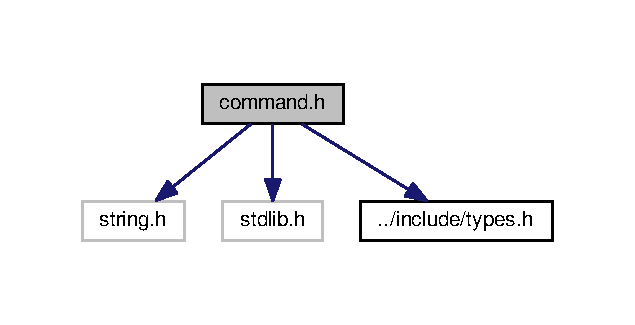
\includegraphics[width=306pt]{command_8h__incl}
\end{center}
\end{figure}
This graph shows which files directly or indirectly include this file\+:\nopagebreak
\begin{figure}[H]
\begin{center}
\leavevmode
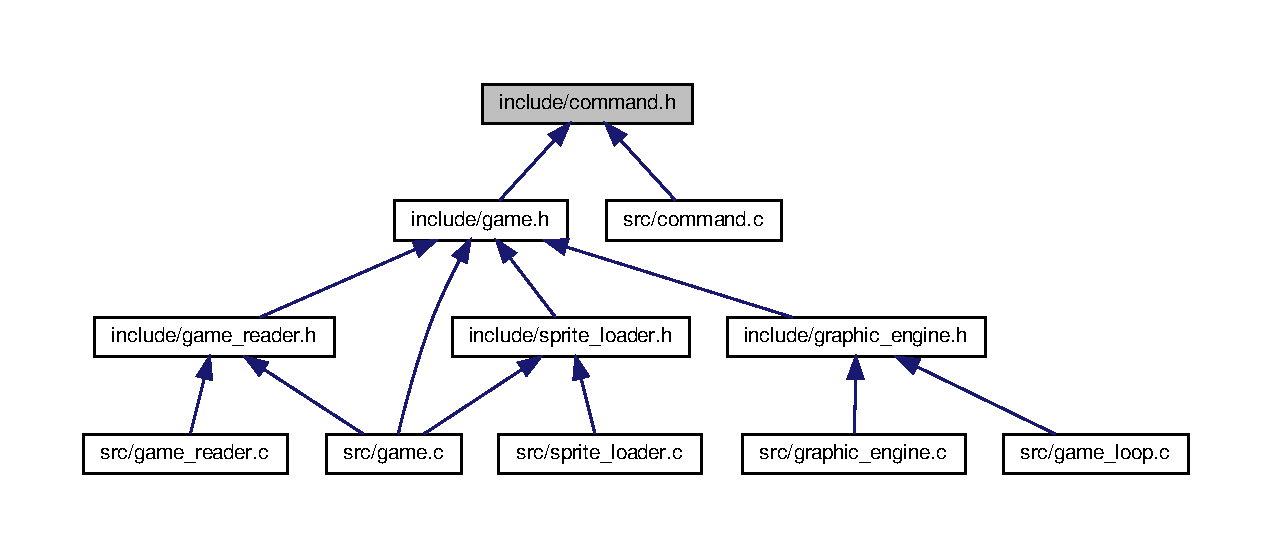
\includegraphics[width=350pt]{command_8h__dep__incl}
\end{center}
\end{figure}
\subsection*{Typedefs}
\begin{DoxyCompactItemize}
\item 
\mbox{\Hypertarget{command_8h_a76085817cb558dc3640088040ba47898}\label{command_8h_a76085817cb558dc3640088040ba47898}} 
typedef struct \hyperlink{struct__F__Command}{\+\_\+\+F\+\_\+\+Command} {\bfseries F\+\_\+\+Command}
\end{DoxyCompactItemize}
\subsection*{Functions}
\begin{DoxyCompactItemize}
\item 
S\+T\+A\+T\+US \hyperlink{command_8h_a8fe217a61bb0d6679328c34b28d8b70c}{get\+\_\+user\+\_\+input} (\hyperlink{struct__F__Command}{F\+\_\+\+Command} $\ast$)
\begin{DoxyCompactList}\small\item\em Stores the input given into a command. \end{DoxyCompactList}\item 
\hyperlink{struct__F__Command}{F\+\_\+\+Command} $\ast$ \hyperlink{command_8h_ae66916e90ab149b0bb6222b1ce60f09b}{command\+\_\+create} ()
\begin{DoxyCompactList}\small\item\em Creates a new F\+\_\+\+Command structure. \end{DoxyCompactList}\item 
void \hyperlink{command_8h_a292bd392485c899b8844fc9fd4d7d196}{command\+\_\+free} (\hyperlink{struct__F__Command}{F\+\_\+\+Command} $\ast$)
\begin{DoxyCompactList}\small\item\em Frees the F\+\_\+\+Command structure. \end{DoxyCompactList}\item 
S\+T\+A\+T\+US \hyperlink{command_8h_a1ec245b7e5700a1ac35b126f31e85671}{command\+\_\+set\+Cmd} (\hyperlink{struct__F__Command}{F\+\_\+\+Command} $\ast$, T\+\_\+\+Command)
\begin{DoxyCompactList}\small\item\em Sets the T\+\_\+\+Command to the one given. \end{DoxyCompactList}\item 
T\+\_\+\+Command \hyperlink{command_8h_a15281f4ecc9fab8fb9fc55273d08742d}{command\+\_\+get\+Cmd} (\hyperlink{struct__F__Command}{F\+\_\+\+Command} $\ast$)
\begin{DoxyCompactList}\small\item\em Gets the T\+\_\+\+Command stored in the F\+\_\+command. \end{DoxyCompactList}\item 
S\+T\+A\+T\+US \hyperlink{command_8h_aaebe404b08dba170b2ec66c5e79ec265}{command\+\_\+set\+\_\+id} (\hyperlink{struct__F__Command}{F\+\_\+\+Command} $\ast$, char $\ast$)
\begin{DoxyCompactList}\small\item\em Sets the parameters of the command given. \end{DoxyCompactList}\item 
char $\ast$ \hyperlink{command_8h_a371627a62bc8e098547786e2c60d6e94}{command\+\_\+get\+\_\+id} (\hyperlink{struct__F__Command}{F\+\_\+\+Command} $\ast$)
\begin{DoxyCompactList}\small\item\em Gets the parameters stored in the F\+\_\+\+Command. \end{DoxyCompactList}\end{DoxyCompactItemize}


\subsection{Detailed Description}
Commands and user input. 

\begin{DoxyAuthor}{Author}
Antonio Solana 
\end{DoxyAuthor}
\begin{DoxyCopyright}{Copyright}
G\+NU Public License 
\end{DoxyCopyright}


\subsection{Function Documentation}
\mbox{\Hypertarget{command_8h_ae66916e90ab149b0bb6222b1ce60f09b}\label{command_8h_ae66916e90ab149b0bb6222b1ce60f09b}} 
\index{command.\+h@{command.\+h}!command\+\_\+create@{command\+\_\+create}}
\index{command\+\_\+create@{command\+\_\+create}!command.\+h@{command.\+h}}
\subsubsection{\texorpdfstring{command\+\_\+create()}{command\_create()}}
{\footnotesize\ttfamily \hyperlink{struct__F__Command}{F\+\_\+\+Command}$\ast$ command\+\_\+create (\begin{DoxyParamCaption}{ }\end{DoxyParamCaption})}



Creates a new F\+\_\+\+Command structure. 

\begin{DoxyAuthor}{Author}
Pablo Sánchez 
\end{DoxyAuthor}
\begin{DoxyReturn}{Returns}
F\+\_\+\+Command$\ast$ new 
\end{DoxyReturn}

\begin{DoxyExceptions}{Exceptions}
{\em Broken} & calloc \\
\hline
\end{DoxyExceptions}
\mbox{\Hypertarget{command_8h_a292bd392485c899b8844fc9fd4d7d196}\label{command_8h_a292bd392485c899b8844fc9fd4d7d196}} 
\index{command.\+h@{command.\+h}!command\+\_\+free@{command\+\_\+free}}
\index{command\+\_\+free@{command\+\_\+free}!command.\+h@{command.\+h}}
\subsubsection{\texorpdfstring{command\+\_\+free()}{command\_free()}}
{\footnotesize\ttfamily void command\+\_\+free (\begin{DoxyParamCaption}\item[{\hyperlink{struct__F__Command}{F\+\_\+\+Command} $\ast$}]{ }\end{DoxyParamCaption})}



Frees the F\+\_\+\+Command structure. 

\begin{DoxyAuthor}{Author}
Pablo Sánchez 
\end{DoxyAuthor}

\begin{DoxyParams}{Parameters}
{\em F\+\_\+\+Command} & to free \\
\hline
\end{DoxyParams}
\mbox{\Hypertarget{command_8h_a371627a62bc8e098547786e2c60d6e94}\label{command_8h_a371627a62bc8e098547786e2c60d6e94}} 
\index{command.\+h@{command.\+h}!command\+\_\+get\+\_\+id@{command\+\_\+get\+\_\+id}}
\index{command\+\_\+get\+\_\+id@{command\+\_\+get\+\_\+id}!command.\+h@{command.\+h}}
\subsubsection{\texorpdfstring{command\+\_\+get\+\_\+id()}{command\_get\_id()}}
{\footnotesize\ttfamily char$\ast$ command\+\_\+get\+\_\+id (\begin{DoxyParamCaption}\item[{\hyperlink{struct__F__Command}{F\+\_\+\+Command} $\ast$}]{ }\end{DoxyParamCaption})}



Gets the parameters stored in the F\+\_\+\+Command. 

\begin{DoxyAuthor}{Author}
Pablo Sánchez 
\end{DoxyAuthor}

\begin{DoxyParams}{Parameters}
{\em F\+\_\+\+Command$\ast$} & \\
\hline
\end{DoxyParams}
\begin{DoxyReturn}{Returns}
char$\ast$ parameters 
\end{DoxyReturn}

\begin{DoxyExceptions}{Exceptions}
{\em No} & F\+\_\+\+Command or value N\+U\+LL \\
\hline
\end{DoxyExceptions}
\mbox{\Hypertarget{command_8h_a15281f4ecc9fab8fb9fc55273d08742d}\label{command_8h_a15281f4ecc9fab8fb9fc55273d08742d}} 
\index{command.\+h@{command.\+h}!command\+\_\+get\+Cmd@{command\+\_\+get\+Cmd}}
\index{command\+\_\+get\+Cmd@{command\+\_\+get\+Cmd}!command.\+h@{command.\+h}}
\subsubsection{\texorpdfstring{command\+\_\+get\+Cmd()}{command\_getCmd()}}
{\footnotesize\ttfamily T\+\_\+\+Command command\+\_\+get\+Cmd (\begin{DoxyParamCaption}\item[{\hyperlink{struct__F__Command}{F\+\_\+\+Command} $\ast$}]{ }\end{DoxyParamCaption})}



Gets the T\+\_\+\+Command stored in the F\+\_\+command. 

\begin{DoxyAuthor}{Author}
Pablo Sánchez 
\end{DoxyAuthor}

\begin{DoxyParams}{Parameters}
{\em F\+\_\+\+Command$\ast$} & \\
\hline
\end{DoxyParams}
\begin{DoxyReturn}{Returns}
T\+\_\+\+Command 
\end{DoxyReturn}

\begin{DoxyExceptions}{Exceptions}
{\em No} & F\+\_\+\+Command or value N\+U\+LL \\
\hline
\end{DoxyExceptions}
\mbox{\Hypertarget{command_8h_aaebe404b08dba170b2ec66c5e79ec265}\label{command_8h_aaebe404b08dba170b2ec66c5e79ec265}} 
\index{command.\+h@{command.\+h}!command\+\_\+set\+\_\+id@{command\+\_\+set\+\_\+id}}
\index{command\+\_\+set\+\_\+id@{command\+\_\+set\+\_\+id}!command.\+h@{command.\+h}}
\subsubsection{\texorpdfstring{command\+\_\+set\+\_\+id()}{command\_set\_id()}}
{\footnotesize\ttfamily S\+T\+A\+T\+US command\+\_\+set\+\_\+id (\begin{DoxyParamCaption}\item[{\hyperlink{struct__F__Command}{F\+\_\+\+Command} $\ast$}]{,  }\item[{char $\ast$}]{ }\end{DoxyParamCaption})}



Sets the parameters of the command given. 

\begin{DoxyAuthor}{Author}
Pablo Sánchez 
\end{DoxyAuthor}

\begin{DoxyParams}{Parameters}
{\em F\+\_\+\+Command$\ast$} & \\
\hline
{\em char$\ast$} & parameters \\
\hline
\end{DoxyParams}
\begin{DoxyReturn}{Returns}
S\+T\+A\+T\+US OK or E\+R\+R\+OR 
\end{DoxyReturn}

\begin{DoxyExceptions}{Exceptions}
{\em NO} & F\+\_\+\+Command or value N\+U\+LL \\
\hline
\end{DoxyExceptions}
\mbox{\Hypertarget{command_8h_a1ec245b7e5700a1ac35b126f31e85671}\label{command_8h_a1ec245b7e5700a1ac35b126f31e85671}} 
\index{command.\+h@{command.\+h}!command\+\_\+set\+Cmd@{command\+\_\+set\+Cmd}}
\index{command\+\_\+set\+Cmd@{command\+\_\+set\+Cmd}!command.\+h@{command.\+h}}
\subsubsection{\texorpdfstring{command\+\_\+set\+Cmd()}{command\_setCmd()}}
{\footnotesize\ttfamily S\+T\+A\+T\+US command\+\_\+set\+Cmd (\begin{DoxyParamCaption}\item[{\hyperlink{struct__F__Command}{F\+\_\+\+Command} $\ast$}]{,  }\item[{T\+\_\+\+Command}]{ }\end{DoxyParamCaption})}



Sets the T\+\_\+\+Command to the one given. 

\begin{DoxyAuthor}{Author}
Pablo Sánchez 
\end{DoxyAuthor}

\begin{DoxyParams}{Parameters}
{\em F\+\_\+\+Command} & $\ast$ \\
\hline
{\em T\+\_\+\+Command} & \\
\hline
\end{DoxyParams}
\begin{DoxyReturn}{Returns}
S\+T\+A\+T\+US OK or E\+R\+R\+OR 
\end{DoxyReturn}

\begin{DoxyExceptions}{Exceptions}
{\em No} & F\+\_\+\+Command or value N\+U\+LL \\
\hline
\end{DoxyExceptions}
\mbox{\Hypertarget{command_8h_a8fe217a61bb0d6679328c34b28d8b70c}\label{command_8h_a8fe217a61bb0d6679328c34b28d8b70c}} 
\index{command.\+h@{command.\+h}!get\+\_\+user\+\_\+input@{get\+\_\+user\+\_\+input}}
\index{get\+\_\+user\+\_\+input@{get\+\_\+user\+\_\+input}!command.\+h@{command.\+h}}
\subsubsection{\texorpdfstring{get\+\_\+user\+\_\+input()}{get\_user\_input()}}
{\footnotesize\ttfamily S\+T\+A\+T\+US get\+\_\+user\+\_\+input (\begin{DoxyParamCaption}\item[{\hyperlink{struct__F__Command}{F\+\_\+\+Command} $\ast$}]{ }\end{DoxyParamCaption})}



Stores the input given into a command. 

\begin{DoxyAuthor}{Author}
Antonio Solana 
\end{DoxyAuthor}

\begin{DoxyParams}{Parameters}
{\em F\+\_\+\+Command$\ast$} & where the command is stored \\
\hline
\end{DoxyParams}
\begin{DoxyReturn}{Returns}
S\+T\+A\+T\+US OK or E\+R\+R\+OR 
\end{DoxyReturn}

\hypertarget{command__test_8c}{}\section{command\+\_\+test.\+c File Reference}
\label{command__test_8c}\index{command\+\_\+test.\+c@{command\+\_\+test.\+c}}
{\ttfamily \#include $<$stdio.\+h$>$}\\*
{\ttfamily \#include $<$stdlib.\+h$>$}\\*
{\ttfamily \#include $<$string.\+h$>$}\\*
{\ttfamily \#include \char`\"{}../include/command.\+h\char`\"{}}\\*
{\ttfamily \#include \char`\"{}../include/command\+\_\+test.\+h\char`\"{}}\\*
{\ttfamily \#include \char`\"{}../include/test.\+h\char`\"{}}\\*
Include dependency graph for command\+\_\+test.\+c\+:\nopagebreak
\begin{figure}[H]
\begin{center}
\leavevmode
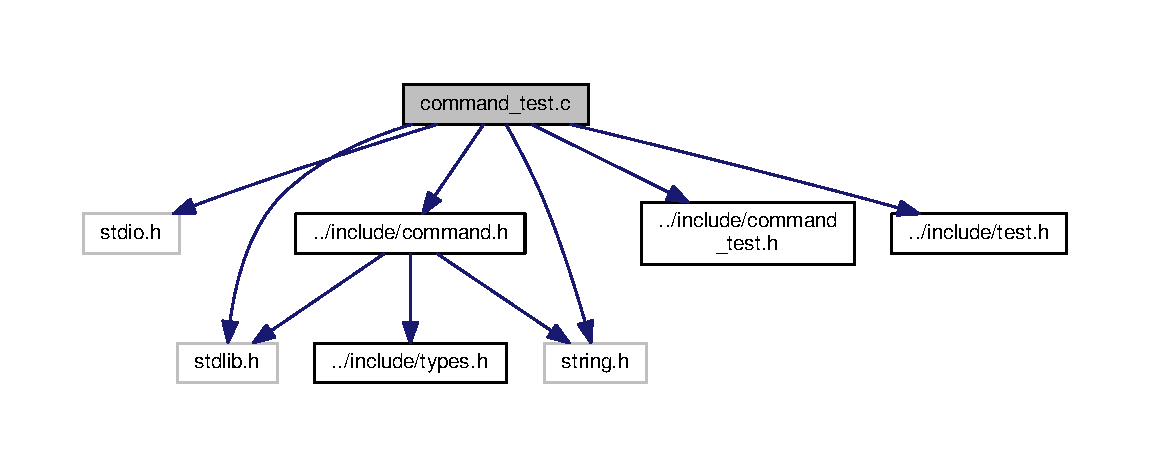
\includegraphics[width=350pt]{command__test_8c__incl}
\end{center}
\end{figure}
\subsection*{Macros}
\begin{DoxyCompactItemize}
\item 
\#define \hyperlink{command__test_8c_a2a77d2f2c5b698c69c19e1f8782bf709}{M\+A\+X\+\_\+\+T\+E\+S\+TS}~8
\end{DoxyCompactItemize}
\subsection*{Functions}
\begin{DoxyCompactItemize}
\item 
int \hyperlink{command__test_8c_a3c04138a5bfe5d72780bb7e82a18e627}{main} (int argc, char $\ast$$\ast$argv)
\begin{DoxyCompactList}\small\item\em Funcion principal de pruebas para el modulo Space. \end{DoxyCompactList}\item 
void \hyperlink{command__test_8c_abed44af325fd42a3f4f4aa134315435c}{test1\+\_\+command\+\_\+create} ()
\item 
void \hyperlink{command__test_8c_ae6bdd5628a9ce9f8dc59f048a63bc34f}{test1\+\_\+command\+\_\+set\+\_\+cmd} ()
\item 
void \hyperlink{command__test_8c_a6d31d85e0bae80d4b3948a15a5b2b00d}{test2\+\_\+command\+\_\+set\+\_\+cmd} ()
\item 
void \hyperlink{command__test_8c_a816316ae397e657bbc52b5b1090d1120}{test1\+\_\+command\+\_\+get\+\_\+cmd} ()
\item 
void \hyperlink{command__test_8c_aca61509275400d7157360abb73218aa1}{test1\+\_\+command\+\_\+set\+\_\+id} ()
\item 
void \hyperlink{command__test_8c_a71ade30f040ea0d0bd3b8a99ef177fac}{test2\+\_\+command\+\_\+set\+\_\+id} ()
\item 
void \hyperlink{command__test_8c_ab23728160ad13bef3d9c5c57b5c34a51}{test1\+\_\+command\+\_\+get\+\_\+id} ()
\end{DoxyCompactItemize}


\subsection{Macro Definition Documentation}
\index{command\+\_\+test.\+c@{command\+\_\+test.\+c}!M\+A\+X\+\_\+\+T\+E\+S\+TS@{M\+A\+X\+\_\+\+T\+E\+S\+TS}}
\index{M\+A\+X\+\_\+\+T\+E\+S\+TS@{M\+A\+X\+\_\+\+T\+E\+S\+TS}!command\+\_\+test.\+c@{command\+\_\+test.\+c}}
\subsubsection[{\texorpdfstring{M\+A\+X\+\_\+\+T\+E\+S\+TS}{MAX_TESTS}}]{\setlength{\rightskip}{0pt plus 5cm}\#define M\+A\+X\+\_\+\+T\+E\+S\+TS~8}\hypertarget{command__test_8c_a2a77d2f2c5b698c69c19e1f8782bf709}{}\label{command__test_8c_a2a77d2f2c5b698c69c19e1f8782bf709}


\subsection{Function Documentation}
\index{command\+\_\+test.\+c@{command\+\_\+test.\+c}!main@{main}}
\index{main@{main}!command\+\_\+test.\+c@{command\+\_\+test.\+c}}
\subsubsection[{\texorpdfstring{main(int argc, char $\ast$$\ast$argv)}{main(int argc, char **argv)}}]{\setlength{\rightskip}{0pt plus 5cm}int main (
\begin{DoxyParamCaption}
\item[{int}]{argc, }
\item[{char $\ast$$\ast$}]{argv}
\end{DoxyParamCaption}
)}\hypertarget{command__test_8c_a3c04138a5bfe5d72780bb7e82a18e627}{}\label{command__test_8c_a3c04138a5bfe5d72780bb7e82a18e627}


Funcion principal de pruebas para el modulo Space. 

Dos modos de ejecucion\+: 1.-\/\+Si se ejecuta sin parametros se ejecutan todas las pruebas 2.-\/\+Si se ejecuta con un numero entre 1 y el numero de pruebas solo ejecuta la prueba indicada \index{command\+\_\+test.\+c@{command\+\_\+test.\+c}!test1\+\_\+command\+\_\+create@{test1\+\_\+command\+\_\+create}}
\index{test1\+\_\+command\+\_\+create@{test1\+\_\+command\+\_\+create}!command\+\_\+test.\+c@{command\+\_\+test.\+c}}
\subsubsection[{\texorpdfstring{test1\+\_\+command\+\_\+create()}{test1_command_create()}}]{\setlength{\rightskip}{0pt plus 5cm}void test1\+\_\+command\+\_\+create (
\begin{DoxyParamCaption}
{}
\end{DoxyParamCaption}
)}\hypertarget{command__test_8c_abed44af325fd42a3f4f4aa134315435c}{}\label{command__test_8c_abed44af325fd42a3f4f4aa134315435c}
\index{command\+\_\+test.\+c@{command\+\_\+test.\+c}!test1\+\_\+command\+\_\+get\+\_\+cmd@{test1\+\_\+command\+\_\+get\+\_\+cmd}}
\index{test1\+\_\+command\+\_\+get\+\_\+cmd@{test1\+\_\+command\+\_\+get\+\_\+cmd}!command\+\_\+test.\+c@{command\+\_\+test.\+c}}
\subsubsection[{\texorpdfstring{test1\+\_\+command\+\_\+get\+\_\+cmd()}{test1_command_get_cmd()}}]{\setlength{\rightskip}{0pt plus 5cm}void test1\+\_\+command\+\_\+get\+\_\+cmd (
\begin{DoxyParamCaption}
{}
\end{DoxyParamCaption}
)}\hypertarget{command__test_8c_a816316ae397e657bbc52b5b1090d1120}{}\label{command__test_8c_a816316ae397e657bbc52b5b1090d1120}
\index{command\+\_\+test.\+c@{command\+\_\+test.\+c}!test1\+\_\+command\+\_\+get\+\_\+id@{test1\+\_\+command\+\_\+get\+\_\+id}}
\index{test1\+\_\+command\+\_\+get\+\_\+id@{test1\+\_\+command\+\_\+get\+\_\+id}!command\+\_\+test.\+c@{command\+\_\+test.\+c}}
\subsubsection[{\texorpdfstring{test1\+\_\+command\+\_\+get\+\_\+id()}{test1_command_get_id()}}]{\setlength{\rightskip}{0pt plus 5cm}void test1\+\_\+command\+\_\+get\+\_\+id (
\begin{DoxyParamCaption}
{}
\end{DoxyParamCaption}
)}\hypertarget{command__test_8c_ab23728160ad13bef3d9c5c57b5c34a51}{}\label{command__test_8c_ab23728160ad13bef3d9c5c57b5c34a51}
\index{command\+\_\+test.\+c@{command\+\_\+test.\+c}!test1\+\_\+command\+\_\+set\+\_\+cmd@{test1\+\_\+command\+\_\+set\+\_\+cmd}}
\index{test1\+\_\+command\+\_\+set\+\_\+cmd@{test1\+\_\+command\+\_\+set\+\_\+cmd}!command\+\_\+test.\+c@{command\+\_\+test.\+c}}
\subsubsection[{\texorpdfstring{test1\+\_\+command\+\_\+set\+\_\+cmd()}{test1_command_set_cmd()}}]{\setlength{\rightskip}{0pt plus 5cm}void test1\+\_\+command\+\_\+set\+\_\+cmd (
\begin{DoxyParamCaption}
{}
\end{DoxyParamCaption}
)}\hypertarget{command__test_8c_ae6bdd5628a9ce9f8dc59f048a63bc34f}{}\label{command__test_8c_ae6bdd5628a9ce9f8dc59f048a63bc34f}
\index{command\+\_\+test.\+c@{command\+\_\+test.\+c}!test1\+\_\+command\+\_\+set\+\_\+id@{test1\+\_\+command\+\_\+set\+\_\+id}}
\index{test1\+\_\+command\+\_\+set\+\_\+id@{test1\+\_\+command\+\_\+set\+\_\+id}!command\+\_\+test.\+c@{command\+\_\+test.\+c}}
\subsubsection[{\texorpdfstring{test1\+\_\+command\+\_\+set\+\_\+id()}{test1_command_set_id()}}]{\setlength{\rightskip}{0pt plus 5cm}void test1\+\_\+command\+\_\+set\+\_\+id (
\begin{DoxyParamCaption}
{}
\end{DoxyParamCaption}
)}\hypertarget{command__test_8c_aca61509275400d7157360abb73218aa1}{}\label{command__test_8c_aca61509275400d7157360abb73218aa1}
\index{command\+\_\+test.\+c@{command\+\_\+test.\+c}!test2\+\_\+command\+\_\+set\+\_\+cmd@{test2\+\_\+command\+\_\+set\+\_\+cmd}}
\index{test2\+\_\+command\+\_\+set\+\_\+cmd@{test2\+\_\+command\+\_\+set\+\_\+cmd}!command\+\_\+test.\+c@{command\+\_\+test.\+c}}
\subsubsection[{\texorpdfstring{test2\+\_\+command\+\_\+set\+\_\+cmd()}{test2_command_set_cmd()}}]{\setlength{\rightskip}{0pt plus 5cm}void test2\+\_\+command\+\_\+set\+\_\+cmd (
\begin{DoxyParamCaption}
{}
\end{DoxyParamCaption}
)}\hypertarget{command__test_8c_a6d31d85e0bae80d4b3948a15a5b2b00d}{}\label{command__test_8c_a6d31d85e0bae80d4b3948a15a5b2b00d}
\index{command\+\_\+test.\+c@{command\+\_\+test.\+c}!test2\+\_\+command\+\_\+set\+\_\+id@{test2\+\_\+command\+\_\+set\+\_\+id}}
\index{test2\+\_\+command\+\_\+set\+\_\+id@{test2\+\_\+command\+\_\+set\+\_\+id}!command\+\_\+test.\+c@{command\+\_\+test.\+c}}
\subsubsection[{\texorpdfstring{test2\+\_\+command\+\_\+set\+\_\+id()}{test2_command_set_id()}}]{\setlength{\rightskip}{0pt plus 5cm}void test2\+\_\+command\+\_\+set\+\_\+id (
\begin{DoxyParamCaption}
{}
\end{DoxyParamCaption}
)}\hypertarget{command__test_8c_a71ade30f040ea0d0bd3b8a99ef177fac}{}\label{command__test_8c_a71ade30f040ea0d0bd3b8a99ef177fac}

\hypertarget{command__test_8h}{}\section{command\+\_\+test.\+h File Reference}
\label{command__test_8h}\index{command\+\_\+test.\+h@{command\+\_\+test.\+h}}


It declares the tests for the command module.  


This graph shows which files directly or indirectly include this file\+:\nopagebreak
\begin{figure}[H]
\begin{center}
\leavevmode
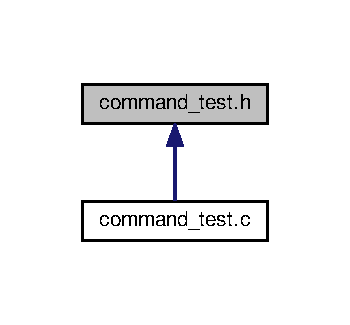
\includegraphics[width=168pt]{command__test_8h__dep__incl}
\end{center}
\end{figure}
\subsection*{Functions}
\begin{DoxyCompactItemize}
\item 
void \hyperlink{command__test_8h_abed44af325fd42a3f4f4aa134315435c}{test1\+\_\+command\+\_\+create} ()
\item 
void \hyperlink{command__test_8h_ae6bdd5628a9ce9f8dc59f048a63bc34f}{test1\+\_\+command\+\_\+set\+\_\+cmd} ()
\item 
void \hyperlink{command__test_8h_a6d31d85e0bae80d4b3948a15a5b2b00d}{test2\+\_\+command\+\_\+set\+\_\+cmd} ()
\item 
void \hyperlink{command__test_8h_a816316ae397e657bbc52b5b1090d1120}{test1\+\_\+command\+\_\+get\+\_\+cmd} ()
\item 
void \hyperlink{command__test_8h_aca61509275400d7157360abb73218aa1}{test1\+\_\+command\+\_\+set\+\_\+id} ()
\item 
void \hyperlink{command__test_8h_a71ade30f040ea0d0bd3b8a99ef177fac}{test2\+\_\+command\+\_\+set\+\_\+id} ()
\item 
void \hyperlink{command__test_8h_ab23728160ad13bef3d9c5c57b5c34a51}{test1\+\_\+command\+\_\+get\+\_\+id} ()
\end{DoxyCompactItemize}


\subsection{Detailed Description}
It declares the tests for the command module. 

\begin{DoxyAuthor}{Author}
Pablo Sánchez Redondo 
\end{DoxyAuthor}
\begin{DoxyCopyright}{Copyright}
G\+NU Public License 
\end{DoxyCopyright}


\subsection{Function Documentation}
\index{command\+\_\+test.\+h@{command\+\_\+test.\+h}!test1\+\_\+command\+\_\+create@{test1\+\_\+command\+\_\+create}}
\index{test1\+\_\+command\+\_\+create@{test1\+\_\+command\+\_\+create}!command\+\_\+test.\+h@{command\+\_\+test.\+h}}
\subsubsection[{\texorpdfstring{test1\+\_\+command\+\_\+create()}{test1_command_create()}}]{\setlength{\rightskip}{0pt plus 5cm}void test1\+\_\+command\+\_\+create (
\begin{DoxyParamCaption}
{}
\end{DoxyParamCaption}
)}\hypertarget{command__test_8h_abed44af325fd42a3f4f4aa134315435c}{}\label{command__test_8h_abed44af325fd42a3f4f4aa134315435c}
\index{command\+\_\+test.\+h@{command\+\_\+test.\+h}!test1\+\_\+command\+\_\+get\+\_\+cmd@{test1\+\_\+command\+\_\+get\+\_\+cmd}}
\index{test1\+\_\+command\+\_\+get\+\_\+cmd@{test1\+\_\+command\+\_\+get\+\_\+cmd}!command\+\_\+test.\+h@{command\+\_\+test.\+h}}
\subsubsection[{\texorpdfstring{test1\+\_\+command\+\_\+get\+\_\+cmd()}{test1_command_get_cmd()}}]{\setlength{\rightskip}{0pt plus 5cm}void test1\+\_\+command\+\_\+get\+\_\+cmd (
\begin{DoxyParamCaption}
{}
\end{DoxyParamCaption}
)}\hypertarget{command__test_8h_a816316ae397e657bbc52b5b1090d1120}{}\label{command__test_8h_a816316ae397e657bbc52b5b1090d1120}
\index{command\+\_\+test.\+h@{command\+\_\+test.\+h}!test1\+\_\+command\+\_\+get\+\_\+id@{test1\+\_\+command\+\_\+get\+\_\+id}}
\index{test1\+\_\+command\+\_\+get\+\_\+id@{test1\+\_\+command\+\_\+get\+\_\+id}!command\+\_\+test.\+h@{command\+\_\+test.\+h}}
\subsubsection[{\texorpdfstring{test1\+\_\+command\+\_\+get\+\_\+id()}{test1_command_get_id()}}]{\setlength{\rightskip}{0pt plus 5cm}void test1\+\_\+command\+\_\+get\+\_\+id (
\begin{DoxyParamCaption}
{}
\end{DoxyParamCaption}
)}\hypertarget{command__test_8h_ab23728160ad13bef3d9c5c57b5c34a51}{}\label{command__test_8h_ab23728160ad13bef3d9c5c57b5c34a51}
\index{command\+\_\+test.\+h@{command\+\_\+test.\+h}!test1\+\_\+command\+\_\+set\+\_\+cmd@{test1\+\_\+command\+\_\+set\+\_\+cmd}}
\index{test1\+\_\+command\+\_\+set\+\_\+cmd@{test1\+\_\+command\+\_\+set\+\_\+cmd}!command\+\_\+test.\+h@{command\+\_\+test.\+h}}
\subsubsection[{\texorpdfstring{test1\+\_\+command\+\_\+set\+\_\+cmd()}{test1_command_set_cmd()}}]{\setlength{\rightskip}{0pt plus 5cm}void test1\+\_\+command\+\_\+set\+\_\+cmd (
\begin{DoxyParamCaption}
{}
\end{DoxyParamCaption}
)}\hypertarget{command__test_8h_ae6bdd5628a9ce9f8dc59f048a63bc34f}{}\label{command__test_8h_ae6bdd5628a9ce9f8dc59f048a63bc34f}
\index{command\+\_\+test.\+h@{command\+\_\+test.\+h}!test1\+\_\+command\+\_\+set\+\_\+id@{test1\+\_\+command\+\_\+set\+\_\+id}}
\index{test1\+\_\+command\+\_\+set\+\_\+id@{test1\+\_\+command\+\_\+set\+\_\+id}!command\+\_\+test.\+h@{command\+\_\+test.\+h}}
\subsubsection[{\texorpdfstring{test1\+\_\+command\+\_\+set\+\_\+id()}{test1_command_set_id()}}]{\setlength{\rightskip}{0pt plus 5cm}void test1\+\_\+command\+\_\+set\+\_\+id (
\begin{DoxyParamCaption}
{}
\end{DoxyParamCaption}
)}\hypertarget{command__test_8h_aca61509275400d7157360abb73218aa1}{}\label{command__test_8h_aca61509275400d7157360abb73218aa1}
\index{command\+\_\+test.\+h@{command\+\_\+test.\+h}!test2\+\_\+command\+\_\+set\+\_\+cmd@{test2\+\_\+command\+\_\+set\+\_\+cmd}}
\index{test2\+\_\+command\+\_\+set\+\_\+cmd@{test2\+\_\+command\+\_\+set\+\_\+cmd}!command\+\_\+test.\+h@{command\+\_\+test.\+h}}
\subsubsection[{\texorpdfstring{test2\+\_\+command\+\_\+set\+\_\+cmd()}{test2_command_set_cmd()}}]{\setlength{\rightskip}{0pt plus 5cm}void test2\+\_\+command\+\_\+set\+\_\+cmd (
\begin{DoxyParamCaption}
{}
\end{DoxyParamCaption}
)}\hypertarget{command__test_8h_a6d31d85e0bae80d4b3948a15a5b2b00d}{}\label{command__test_8h_a6d31d85e0bae80d4b3948a15a5b2b00d}
\index{command\+\_\+test.\+h@{command\+\_\+test.\+h}!test2\+\_\+command\+\_\+set\+\_\+id@{test2\+\_\+command\+\_\+set\+\_\+id}}
\index{test2\+\_\+command\+\_\+set\+\_\+id@{test2\+\_\+command\+\_\+set\+\_\+id}!command\+\_\+test.\+h@{command\+\_\+test.\+h}}
\subsubsection[{\texorpdfstring{test2\+\_\+command\+\_\+set\+\_\+id()}{test2_command_set_id()}}]{\setlength{\rightskip}{0pt plus 5cm}void test2\+\_\+command\+\_\+set\+\_\+id (
\begin{DoxyParamCaption}
{}
\end{DoxyParamCaption}
)}\hypertarget{command__test_8h_a71ade30f040ea0d0bd3b8a99ef177fac}{}\label{command__test_8h_a71ade30f040ea0d0bd3b8a99ef177fac}

\hypertarget{die_8c}{\section{die.\+c File Reference}
\label{die_8c}\index{die.\+c@{die.\+c}}
}


It declares the die module.  


{\ttfamily \#include \char`\"{}../include/die.\+h\char`\"{}}\\*
Include dependency graph for die.\+c\+:\nopagebreak
\begin{figure}[H]
\begin{center}
\leavevmode
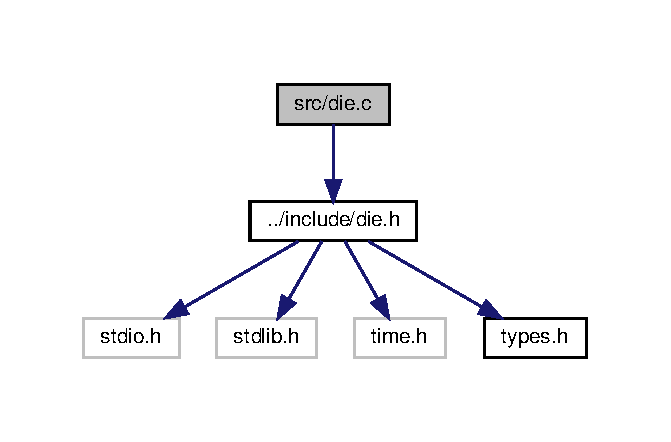
\includegraphics[width=321pt]{die_8c__incl}
\end{center}
\end{figure}
\subsection*{Classes}
\begin{DoxyCompactItemize}
\item 
struct \hyperlink{struct__Die}{\+\_\+\+Die}
\end{DoxyCompactItemize}
\subsection*{Functions}
\begin{DoxyCompactItemize}
\item 
\hyperlink{die_8h_a892f0b0bf81d69a1f7a14ea238e36dd3}{Die} $\ast$ \hyperlink{die_8c_ad5714ba396ffc8c964b7be67240508b2}{die\+\_\+ini} (\hyperlink{types_8h_a845e604fb28f7e3d97549da3448149d3}{Id} id)
\begin{DoxyCompactList}\small\item\em esta funcion se encarga de crear el dado reservando memoria para el mismo. \end{DoxyCompactList}\item 
void \hyperlink{die_8c_aa8e971f9b27132eda0d1e8177adc7ed5}{die\+\_\+die\+\_\+die} (\hyperlink{die_8h_a892f0b0bf81d69a1f7a14ea238e36dd3}{Die} $\ast$die)
\begin{DoxyCompactList}\small\item\em Destruye el dado recibido. \end{DoxyCompactList}\item 
\hyperlink{types_8h_a32c27cc471df37f4fc818d65de0a56c4}{S\+T\+A\+T\+U\+S} \hyperlink{die_8c_afafc56aafeb40dbf889c421cace3d919}{die\+\_\+roll} (\hyperlink{die_8h_a892f0b0bf81d69a1f7a14ea238e36dd3}{Die} $\ast$die)
\begin{DoxyCompactList}\small\item\em esta funcion se encarga de llamar a la funcion aleatorio() para simular la tirada del dado y devolver el numero elegido \end{DoxyCompactList}\item 
\hyperlink{types_8h_a32c27cc471df37f4fc818d65de0a56c4}{S\+T\+A\+T\+U\+S} \hyperlink{die_8c_a4ba0de5e507530e14302ac5096d7df56}{die\+\_\+print} (F\+I\+L\+E $\ast$f, \hyperlink{die_8h_a892f0b0bf81d69a1f7a14ea238e36dd3}{Die} $\ast$die)
\begin{DoxyCompactList}\small\item\em esta funcion se encarga de imprimir el contenido del dado \end{DoxyCompactList}\item 
short int \hyperlink{die_8c_a734148bcd7a5fc018966fa3b7909ac4a}{die\+\_\+get\+\_\+last\+\_\+roll} (\hyperlink{die_8h_a892f0b0bf81d69a1f7a14ea238e36dd3}{Die} $\ast$die)
\begin{DoxyCompactList}\small\item\em consigue el valor de la ultima tirada \end{DoxyCompactList}\end{DoxyCompactItemize}


\subsection{Detailed Description}
It declares the die module. 

\begin{DoxyAuthor}{Author}
Pablo Sánchez Redondo 
\end{DoxyAuthor}
\begin{DoxyCopyright}{Copyright}
G\+N\+U Public License 
\end{DoxyCopyright}


\subsection{Function Documentation}
\hypertarget{die_8c_aa8e971f9b27132eda0d1e8177adc7ed5}{\index{die.\+c@{die.\+c}!die\+\_\+die\+\_\+die@{die\+\_\+die\+\_\+die}}
\index{die\+\_\+die\+\_\+die@{die\+\_\+die\+\_\+die}!die.\+c@{die.\+c}}
\subsubsection[{die\+\_\+die\+\_\+die}]{\setlength{\rightskip}{0pt plus 5cm}void die\+\_\+die\+\_\+die (
\begin{DoxyParamCaption}
\item[{{\bf Die} $\ast$}]{}
\end{DoxyParamCaption}
)}}\label{die_8c_aa8e971f9b27132eda0d1e8177adc7ed5}


Destruye el dado recibido. 

\begin{DoxyAuthor}{Author}
Pablo Sánchez 
\end{DoxyAuthor}

\begin{DoxyParams}{Parameters}
{\em $\ast$\+Die} & \\
\hline
\end{DoxyParams}
\hypertarget{die_8c_a734148bcd7a5fc018966fa3b7909ac4a}{\index{die.\+c@{die.\+c}!die\+\_\+get\+\_\+last\+\_\+roll@{die\+\_\+get\+\_\+last\+\_\+roll}}
\index{die\+\_\+get\+\_\+last\+\_\+roll@{die\+\_\+get\+\_\+last\+\_\+roll}!die.\+c@{die.\+c}}
\subsubsection[{die\+\_\+get\+\_\+last\+\_\+roll}]{\setlength{\rightskip}{0pt plus 5cm}short int die\+\_\+get\+\_\+last\+\_\+roll (
\begin{DoxyParamCaption}
\item[{{\bf Die} $\ast$}]{}
\end{DoxyParamCaption}
)}}\label{die_8c_a734148bcd7a5fc018966fa3b7909ac4a}


consigue el valor de la ultima tirada 

\begin{DoxyAuthor}{Author}
Pablo Sánchez  Die$\ast$ 
\end{DoxyAuthor}
\begin{DoxyReturn}{Returns}
short int la ultima tirada 
\end{DoxyReturn}
\hypertarget{die_8c_ad5714ba396ffc8c964b7be67240508b2}{\index{die.\+c@{die.\+c}!die\+\_\+ini@{die\+\_\+ini}}
\index{die\+\_\+ini@{die\+\_\+ini}!die.\+c@{die.\+c}}
\subsubsection[{die\+\_\+ini}]{\setlength{\rightskip}{0pt plus 5cm}{\bf Die}$\ast$ die\+\_\+ini (
\begin{DoxyParamCaption}
\item[{{\bf Id}}]{}
\end{DoxyParamCaption}
)}}\label{die_8c_ad5714ba396ffc8c964b7be67240508b2}


esta funcion se encarga de crear el dado reservando memoria para el mismo. 

\begin{DoxyAuthor}{Author}
Pablo Sánchez  I\+D, el id del dado. 
\end{DoxyAuthor}
\begin{DoxyReturn}{Returns}
newdie, el dado creado, o N\+U\+L\+L si algo no ha salido como esperaba. 
\end{DoxyReturn}
\hypertarget{die_8c_a4ba0de5e507530e14302ac5096d7df56}{\index{die.\+c@{die.\+c}!die\+\_\+print@{die\+\_\+print}}
\index{die\+\_\+print@{die\+\_\+print}!die.\+c@{die.\+c}}
\subsubsection[{die\+\_\+print}]{\setlength{\rightskip}{0pt plus 5cm}{\bf S\+T\+A\+T\+U\+S} die\+\_\+print (
\begin{DoxyParamCaption}
\item[{F\+I\+L\+E $\ast$}]{, }
\item[{{\bf Die} $\ast$}]{}
\end{DoxyParamCaption}
)}}\label{die_8c_a4ba0de5e507530e14302ac5096d7df56}


esta funcion se encarga de imprimir el contenido del dado 

\begin{DoxyAuthor}{Author}
Pablo Sánchez  Die$\ast$die, el dado que desea imprimir. 
\end{DoxyAuthor}
\begin{DoxyReturn}{Returns}
E\+R\+R\+O\+R si algo no ha salido como se esperaba. 
\end{DoxyReturn}
\hypertarget{die_8c_afafc56aafeb40dbf889c421cace3d919}{\index{die.\+c@{die.\+c}!die\+\_\+roll@{die\+\_\+roll}}
\index{die\+\_\+roll@{die\+\_\+roll}!die.\+c@{die.\+c}}
\subsubsection[{die\+\_\+roll}]{\setlength{\rightskip}{0pt plus 5cm}{\bf S\+T\+A\+T\+U\+S} die\+\_\+roll (
\begin{DoxyParamCaption}
\item[{{\bf Die} $\ast$}]{}
\end{DoxyParamCaption}
)}}\label{die_8c_afafc56aafeb40dbf889c421cace3d919}


esta funcion se encarga de llamar a la funcion aleatorio() para simular la tirada del dado y devolver el numero elegido 

\begin{DoxyAuthor}{Author}
Pablo Sánchez 
\end{DoxyAuthor}
\begin{DoxyReturn}{Returns}
Die=$>$ult\+\_\+tirada si ha salido correctamente o E\+R\+R\+O\+R si no. 
\end{DoxyReturn}

\hypertarget{die_8h}{}\section{include/die.h File Reference}
\label{die_8h}\index{include/die.\+h@{include/die.\+h}}


It declares the die module.  


{\ttfamily \#include $<$stdio.\+h$>$}\newline
{\ttfamily \#include $<$stdlib.\+h$>$}\newline
{\ttfamily \#include $<$time.\+h$>$}\newline
{\ttfamily \#include \char`\"{}types.\+h\char`\"{}}\newline
Include dependency graph for die.\+h\+:\nopagebreak
\begin{figure}[H]
\begin{center}
\leavevmode
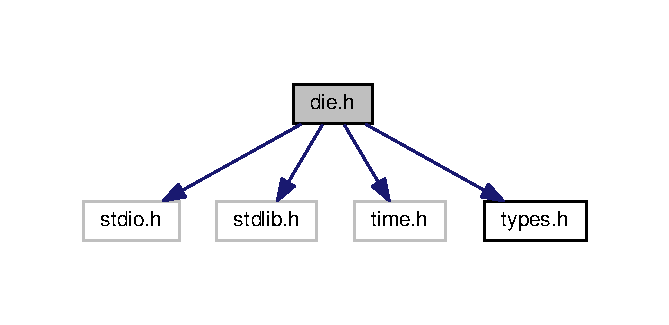
\includegraphics[width=322pt]{die_8h__incl}
\end{center}
\end{figure}
This graph shows which files directly or indirectly include this file\+:\nopagebreak
\begin{figure}[H]
\begin{center}
\leavevmode
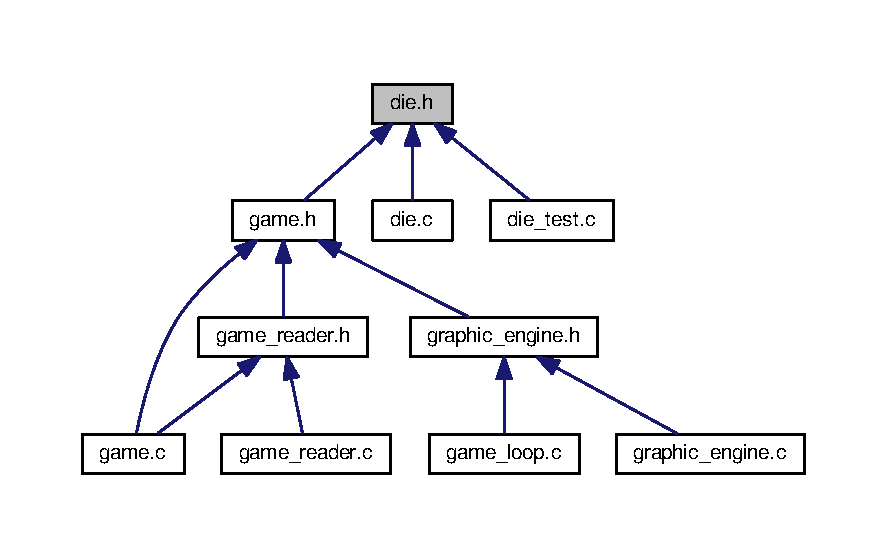
\includegraphics[width=350pt]{die_8h__dep__incl}
\end{center}
\end{figure}
\subsection*{Typedefs}
\begin{DoxyCompactItemize}
\item 
typedef struct \hyperlink{struct__Die}{\+\_\+\+Die} \hyperlink{die_8h_a892f0b0bf81d69a1f7a14ea238e36dd3}{Die}
\end{DoxyCompactItemize}
\subsection*{Functions}
\begin{DoxyCompactItemize}
\item 
\hyperlink{die_8h_a892f0b0bf81d69a1f7a14ea238e36dd3}{Die} $\ast$ \hyperlink{die_8h_a58ac2859cec9338bd57d2cbf142f565f}{die\+\_\+ini} (Id)
\begin{DoxyCompactList}\small\item\em esta funcion se encarga de crear el dado reservando memoria para el mismo. \end{DoxyCompactList}\item 
void \hyperlink{die_8h_a94ea40d2a3508e2d6aac560582e9e9bc}{die\+\_\+die\+\_\+die} (\hyperlink{die_8h_a892f0b0bf81d69a1f7a14ea238e36dd3}{Die} $\ast$)
\begin{DoxyCompactList}\small\item\em Destruye el dado recibido. \end{DoxyCompactList}\item 
S\+T\+A\+T\+US \hyperlink{die_8h_a8b747943478f695a940e267d69baae7b}{die\+\_\+roll} (\hyperlink{die_8h_a892f0b0bf81d69a1f7a14ea238e36dd3}{Die} $\ast$)
\begin{DoxyCompactList}\small\item\em esta funcion se encarga de llamar a la funcion aleatorio() para simular la tirada del dado y devolver el numero elegido \end{DoxyCompactList}\item 
short int \hyperlink{die_8h_a8bf4da5fb5440c903b605e54ceae97e5}{die\+\_\+get\+\_\+last\+\_\+roll} (\hyperlink{die_8h_a892f0b0bf81d69a1f7a14ea238e36dd3}{Die} $\ast$)
\begin{DoxyCompactList}\small\item\em consigue el valor de la ultima tirada \end{DoxyCompactList}\item 
S\+T\+A\+T\+US \hyperlink{die_8h_ac5fb013351c7196f7ace1ac1043771fc}{die\+\_\+print} (F\+I\+LE $\ast$, \hyperlink{die_8h_a892f0b0bf81d69a1f7a14ea238e36dd3}{Die} $\ast$)
\begin{DoxyCompactList}\small\item\em esta funcion se encarga de imprimir el contenido del dado \end{DoxyCompactList}\end{DoxyCompactItemize}


\subsection{Detailed Description}
It declares the die module. 

\begin{DoxyAuthor}{Author}
Pablo Sánchez 
\end{DoxyAuthor}
\begin{DoxyCopyright}{Copyright}
G\+NU Public License 
\end{DoxyCopyright}


\subsection{Typedef Documentation}
\mbox{\Hypertarget{die_8h_a892f0b0bf81d69a1f7a14ea238e36dd3}\label{die_8h_a892f0b0bf81d69a1f7a14ea238e36dd3}} 
\index{die.\+h@{die.\+h}!Die@{Die}}
\index{Die@{Die}!die.\+h@{die.\+h}}
\subsubsection{\texorpdfstring{Die}{Die}}
{\footnotesize\ttfamily typedef struct \hyperlink{struct__Die}{\+\_\+\+Die} \hyperlink{die_8h_a892f0b0bf81d69a1f7a14ea238e36dd3}{Die}}

la estructura \hyperlink{struct__Die}{\+\_\+\+Die} consta de dos componentes, uno de ellos, ID (donde se guardara el id de los dados) e int ult\+\_\+tirada (donde se guarda el ultimo resultado de la funcion roll\+\_\+die() ). 

\subsection{Function Documentation}
\mbox{\Hypertarget{die_8h_a94ea40d2a3508e2d6aac560582e9e9bc}\label{die_8h_a94ea40d2a3508e2d6aac560582e9e9bc}} 
\index{die.\+h@{die.\+h}!die\+\_\+die\+\_\+die@{die\+\_\+die\+\_\+die}}
\index{die\+\_\+die\+\_\+die@{die\+\_\+die\+\_\+die}!die.\+h@{die.\+h}}
\subsubsection{\texorpdfstring{die\+\_\+die\+\_\+die()}{die\_die\_die()}}
{\footnotesize\ttfamily void die\+\_\+die\+\_\+die (\begin{DoxyParamCaption}\item[{\hyperlink{die_8h_a892f0b0bf81d69a1f7a14ea238e36dd3}{Die} $\ast$}]{ }\end{DoxyParamCaption})}



Destruye el dado recibido. 

\begin{DoxyAuthor}{Author}
Pablo Sánchez 
\end{DoxyAuthor}

\begin{DoxyParams}{Parameters}
{\em $\ast$\+Die} & \\
\hline
\end{DoxyParams}
\mbox{\Hypertarget{die_8h_a8bf4da5fb5440c903b605e54ceae97e5}\label{die_8h_a8bf4da5fb5440c903b605e54ceae97e5}} 
\index{die.\+h@{die.\+h}!die\+\_\+get\+\_\+last\+\_\+roll@{die\+\_\+get\+\_\+last\+\_\+roll}}
\index{die\+\_\+get\+\_\+last\+\_\+roll@{die\+\_\+get\+\_\+last\+\_\+roll}!die.\+h@{die.\+h}}
\subsubsection{\texorpdfstring{die\+\_\+get\+\_\+last\+\_\+roll()}{die\_get\_last\_roll()}}
{\footnotesize\ttfamily short int die\+\_\+get\+\_\+last\+\_\+roll (\begin{DoxyParamCaption}\item[{\hyperlink{die_8h_a892f0b0bf81d69a1f7a14ea238e36dd3}{Die} $\ast$}]{ }\end{DoxyParamCaption})}



consigue el valor de la ultima tirada 

\begin{DoxyAuthor}{Author}
Pablo Sánchez  Die$\ast$ 
\end{DoxyAuthor}
\begin{DoxyReturn}{Returns}
short int la ultima tirada 
\end{DoxyReturn}
\mbox{\Hypertarget{die_8h_a58ac2859cec9338bd57d2cbf142f565f}\label{die_8h_a58ac2859cec9338bd57d2cbf142f565f}} 
\index{die.\+h@{die.\+h}!die\+\_\+ini@{die\+\_\+ini}}
\index{die\+\_\+ini@{die\+\_\+ini}!die.\+h@{die.\+h}}
\subsubsection{\texorpdfstring{die\+\_\+ini()}{die\_ini()}}
{\footnotesize\ttfamily \hyperlink{die_8h_a892f0b0bf81d69a1f7a14ea238e36dd3}{Die}$\ast$ die\+\_\+ini (\begin{DoxyParamCaption}\item[{Id}]{ }\end{DoxyParamCaption})}



esta funcion se encarga de crear el dado reservando memoria para el mismo. 

\begin{DoxyAuthor}{Author}
Pablo Sánchez  ID, el id del dado. 
\end{DoxyAuthor}
\begin{DoxyReturn}{Returns}
newdie, el dado creado, o N\+U\+LL si algo no ha salido como esperaba. 
\end{DoxyReturn}
\mbox{\Hypertarget{die_8h_ac5fb013351c7196f7ace1ac1043771fc}\label{die_8h_ac5fb013351c7196f7ace1ac1043771fc}} 
\index{die.\+h@{die.\+h}!die\+\_\+print@{die\+\_\+print}}
\index{die\+\_\+print@{die\+\_\+print}!die.\+h@{die.\+h}}
\subsubsection{\texorpdfstring{die\+\_\+print()}{die\_print()}}
{\footnotesize\ttfamily S\+T\+A\+T\+US die\+\_\+print (\begin{DoxyParamCaption}\item[{F\+I\+LE $\ast$}]{,  }\item[{\hyperlink{die_8h_a892f0b0bf81d69a1f7a14ea238e36dd3}{Die} $\ast$}]{ }\end{DoxyParamCaption})}



esta funcion se encarga de imprimir el contenido del dado 

\begin{DoxyAuthor}{Author}
Pablo Sánchez  Die$\ast$die, el dado que desea imprimir. 
\end{DoxyAuthor}
\begin{DoxyReturn}{Returns}
E\+R\+R\+OR si algo no ha salido como se esperaba. 
\end{DoxyReturn}
\mbox{\Hypertarget{die_8h_a8b747943478f695a940e267d69baae7b}\label{die_8h_a8b747943478f695a940e267d69baae7b}} 
\index{die.\+h@{die.\+h}!die\+\_\+roll@{die\+\_\+roll}}
\index{die\+\_\+roll@{die\+\_\+roll}!die.\+h@{die.\+h}}
\subsubsection{\texorpdfstring{die\+\_\+roll()}{die\_roll()}}
{\footnotesize\ttfamily S\+T\+A\+T\+US die\+\_\+roll (\begin{DoxyParamCaption}\item[{\hyperlink{die_8h_a892f0b0bf81d69a1f7a14ea238e36dd3}{Die} $\ast$}]{ }\end{DoxyParamCaption})}



esta funcion se encarga de llamar a la funcion aleatorio() para simular la tirada del dado y devolver el numero elegido 

\begin{DoxyAuthor}{Author}
Pablo Sánchez 
\end{DoxyAuthor}
\begin{DoxyReturn}{Returns}
Die=$>$ult\+\_\+tirada si ha salido correctamente o E\+R\+R\+OR si no. 
\end{DoxyReturn}

\hypertarget{die__test_8c}{\section{die\+\_\+test.\+c File Reference}
\label{die__test_8c}\index{die\+\_\+test.\+c@{die\+\_\+test.\+c}}
}
{\ttfamily \#include $<$stdio.\+h$>$}\\*
{\ttfamily \#include $<$stdlib.\+h$>$}\\*
{\ttfamily \#include $<$string.\+h$>$}\\*
{\ttfamily \#include \char`\"{}../include/die.\+h\char`\"{}}\\*
{\ttfamily \#include \char`\"{}../include/die\+\_\+test.\+h\char`\"{}}\\*
{\ttfamily \#include \char`\"{}../include/test.\+h\char`\"{}}\\*
Include dependency graph for die\+\_\+test.\+c\+:\nopagebreak
\begin{figure}[H]
\begin{center}
\leavevmode
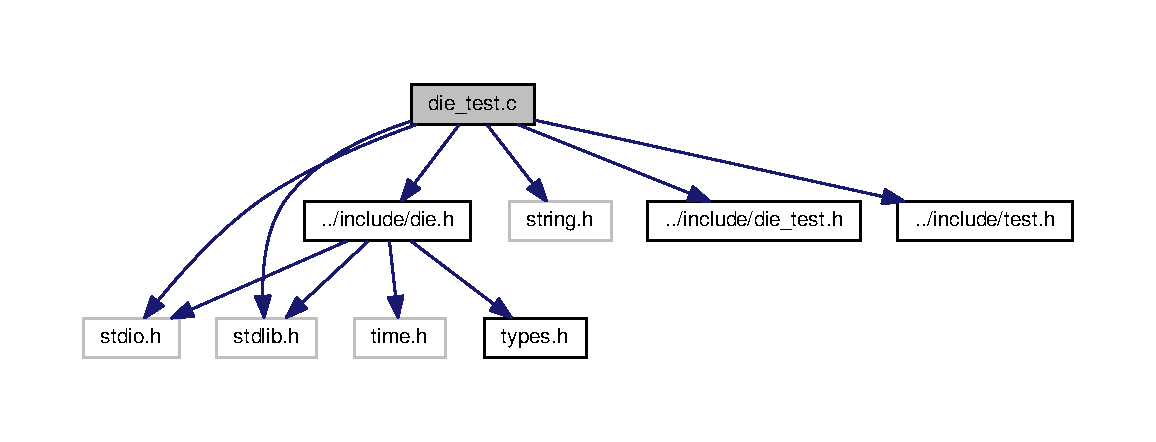
\includegraphics[width=350pt]{die__test_8c__incl}
\end{center}
\end{figure}
\subsection*{Macros}
\begin{DoxyCompactItemize}
\item 
\#define \hyperlink{die__test_8c_a2a77d2f2c5b698c69c19e1f8782bf709}{M\+A\+X\+\_\+\+T\+E\+S\+T\+S}~6
\end{DoxyCompactItemize}
\subsection*{Functions}
\begin{DoxyCompactItemize}
\item 
int \hyperlink{die__test_8c_a3c04138a5bfe5d72780bb7e82a18e627}{main} (int argc, char $\ast$$\ast$argv)
\begin{DoxyCompactList}\small\item\em Funcion principal de pruebas para el modulo Space. \end{DoxyCompactList}\item 
void \hyperlink{die__test_8c_ac0b610468bd3d3b358051c966b771431}{test1\+\_\+die\+\_\+create} ()
\item 
void \hyperlink{die__test_8c_ac005cb42fa33b38a79896934a5a50001}{test1\+\_\+die\+\_\+roll} ()
\item 
void \hyperlink{die__test_8c_af7df60d905acf9505f1e434c6f75d027}{test2\+\_\+die\+\_\+roll} ()
\item 
void \hyperlink{die__test_8c_a99e873ecce6a19186919e991876dadbe}{test1\+\_\+die\+\_\+get\+\_\+last\+\_\+roll} ()
\item 
void \hyperlink{die__test_8c_a0832aa306964705770b2f1240763d962}{test2\+\_\+die\+\_\+get\+\_\+last\+\_\+roll} ()
\end{DoxyCompactItemize}


\subsection{Macro Definition Documentation}
\hypertarget{die__test_8c_a2a77d2f2c5b698c69c19e1f8782bf709}{\index{die\+\_\+test.\+c@{die\+\_\+test.\+c}!M\+A\+X\+\_\+\+T\+E\+S\+T\+S@{M\+A\+X\+\_\+\+T\+E\+S\+T\+S}}
\index{M\+A\+X\+\_\+\+T\+E\+S\+T\+S@{M\+A\+X\+\_\+\+T\+E\+S\+T\+S}!die\+\_\+test.\+c@{die\+\_\+test.\+c}}
\subsubsection[{M\+A\+X\+\_\+\+T\+E\+S\+T\+S}]{\setlength{\rightskip}{0pt plus 5cm}\#define M\+A\+X\+\_\+\+T\+E\+S\+T\+S~6}}\label{die__test_8c_a2a77d2f2c5b698c69c19e1f8782bf709}


\subsection{Function Documentation}
\hypertarget{die__test_8c_a3c04138a5bfe5d72780bb7e82a18e627}{\index{die\+\_\+test.\+c@{die\+\_\+test.\+c}!main@{main}}
\index{main@{main}!die\+\_\+test.\+c@{die\+\_\+test.\+c}}
\subsubsection[{main}]{\setlength{\rightskip}{0pt plus 5cm}int main (
\begin{DoxyParamCaption}
\item[{int}]{argc, }
\item[{char $\ast$$\ast$}]{argv}
\end{DoxyParamCaption}
)}}\label{die__test_8c_a3c04138a5bfe5d72780bb7e82a18e627}


Funcion principal de pruebas para el modulo Space. 

Dos modos de ejecucion\+: 1.-\/\+Si se ejecuta sin parametros se ejecutan todas las pruebas 2.-\/\+Si se ejecuta con un numero entre 1 y el numero de pruebas solo ejecuta la prueba indicada \hypertarget{die__test_8c_ac0b610468bd3d3b358051c966b771431}{\index{die\+\_\+test.\+c@{die\+\_\+test.\+c}!test1\+\_\+die\+\_\+create@{test1\+\_\+die\+\_\+create}}
\index{test1\+\_\+die\+\_\+create@{test1\+\_\+die\+\_\+create}!die\+\_\+test.\+c@{die\+\_\+test.\+c}}
\subsubsection[{test1\+\_\+die\+\_\+create}]{\setlength{\rightskip}{0pt plus 5cm}void test1\+\_\+die\+\_\+create (
\begin{DoxyParamCaption}
{}
\end{DoxyParamCaption}
)}}\label{die__test_8c_ac0b610468bd3d3b358051c966b771431}
\hypertarget{die__test_8c_a99e873ecce6a19186919e991876dadbe}{\index{die\+\_\+test.\+c@{die\+\_\+test.\+c}!test1\+\_\+die\+\_\+get\+\_\+last\+\_\+roll@{test1\+\_\+die\+\_\+get\+\_\+last\+\_\+roll}}
\index{test1\+\_\+die\+\_\+get\+\_\+last\+\_\+roll@{test1\+\_\+die\+\_\+get\+\_\+last\+\_\+roll}!die\+\_\+test.\+c@{die\+\_\+test.\+c}}
\subsubsection[{test1\+\_\+die\+\_\+get\+\_\+last\+\_\+roll}]{\setlength{\rightskip}{0pt plus 5cm}void test1\+\_\+die\+\_\+get\+\_\+last\+\_\+roll (
\begin{DoxyParamCaption}
{}
\end{DoxyParamCaption}
)}}\label{die__test_8c_a99e873ecce6a19186919e991876dadbe}
\hypertarget{die__test_8c_ac005cb42fa33b38a79896934a5a50001}{\index{die\+\_\+test.\+c@{die\+\_\+test.\+c}!test1\+\_\+die\+\_\+roll@{test1\+\_\+die\+\_\+roll}}
\index{test1\+\_\+die\+\_\+roll@{test1\+\_\+die\+\_\+roll}!die\+\_\+test.\+c@{die\+\_\+test.\+c}}
\subsubsection[{test1\+\_\+die\+\_\+roll}]{\setlength{\rightskip}{0pt plus 5cm}void test1\+\_\+die\+\_\+roll (
\begin{DoxyParamCaption}
{}
\end{DoxyParamCaption}
)}}\label{die__test_8c_ac005cb42fa33b38a79896934a5a50001}
\hypertarget{die__test_8c_a0832aa306964705770b2f1240763d962}{\index{die\+\_\+test.\+c@{die\+\_\+test.\+c}!test2\+\_\+die\+\_\+get\+\_\+last\+\_\+roll@{test2\+\_\+die\+\_\+get\+\_\+last\+\_\+roll}}
\index{test2\+\_\+die\+\_\+get\+\_\+last\+\_\+roll@{test2\+\_\+die\+\_\+get\+\_\+last\+\_\+roll}!die\+\_\+test.\+c@{die\+\_\+test.\+c}}
\subsubsection[{test2\+\_\+die\+\_\+get\+\_\+last\+\_\+roll}]{\setlength{\rightskip}{0pt plus 5cm}void test2\+\_\+die\+\_\+get\+\_\+last\+\_\+roll (
\begin{DoxyParamCaption}
{}
\end{DoxyParamCaption}
)}}\label{die__test_8c_a0832aa306964705770b2f1240763d962}
\hypertarget{die__test_8c_af7df60d905acf9505f1e434c6f75d027}{\index{die\+\_\+test.\+c@{die\+\_\+test.\+c}!test2\+\_\+die\+\_\+roll@{test2\+\_\+die\+\_\+roll}}
\index{test2\+\_\+die\+\_\+roll@{test2\+\_\+die\+\_\+roll}!die\+\_\+test.\+c@{die\+\_\+test.\+c}}
\subsubsection[{test2\+\_\+die\+\_\+roll}]{\setlength{\rightskip}{0pt plus 5cm}void test2\+\_\+die\+\_\+roll (
\begin{DoxyParamCaption}
{}
\end{DoxyParamCaption}
)}}\label{die__test_8c_af7df60d905acf9505f1e434c6f75d027}

\hypertarget{die__test_8h}{}\section{die\+\_\+test.\+h File Reference}
\label{die__test_8h}\index{die\+\_\+test.\+h@{die\+\_\+test.\+h}}


It declares the tests for the die module.  


This graph shows which files directly or indirectly include this file\+:\nopagebreak
\begin{figure}[H]
\begin{center}
\leavevmode
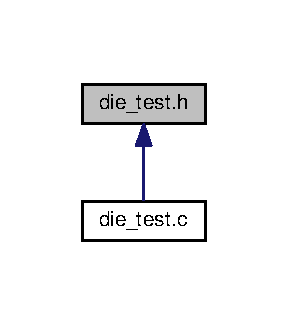
\includegraphics[width=138pt]{die__test_8h__dep__incl}
\end{center}
\end{figure}
\subsection*{Functions}
\begin{DoxyCompactItemize}
\item 
void \hyperlink{die__test_8h_ac0b610468bd3d3b358051c966b771431}{test1\+\_\+die\+\_\+create} ()
\item 
void \hyperlink{die__test_8h_ac005cb42fa33b38a79896934a5a50001}{test1\+\_\+die\+\_\+roll} ()
\item 
void \hyperlink{die__test_8h_af7df60d905acf9505f1e434c6f75d027}{test2\+\_\+die\+\_\+roll} ()
\item 
void \hyperlink{die__test_8h_a99e873ecce6a19186919e991876dadbe}{test1\+\_\+die\+\_\+get\+\_\+last\+\_\+roll} ()
\item 
void \hyperlink{die__test_8h_a0832aa306964705770b2f1240763d962}{test2\+\_\+die\+\_\+get\+\_\+last\+\_\+roll} ()
\end{DoxyCompactItemize}


\subsection{Detailed Description}
It declares the tests for the die module. 

\begin{DoxyAuthor}{Author}
Pablo Sánchez Redondo 
\end{DoxyAuthor}
\begin{DoxyCopyright}{Copyright}
G\+NU Public License 
\end{DoxyCopyright}


\subsection{Function Documentation}
\index{die\+\_\+test.\+h@{die\+\_\+test.\+h}!test1\+\_\+die\+\_\+create@{test1\+\_\+die\+\_\+create}}
\index{test1\+\_\+die\+\_\+create@{test1\+\_\+die\+\_\+create}!die\+\_\+test.\+h@{die\+\_\+test.\+h}}
\subsubsection[{\texorpdfstring{test1\+\_\+die\+\_\+create()}{test1_die_create()}}]{\setlength{\rightskip}{0pt plus 5cm}void test1\+\_\+die\+\_\+create (
\begin{DoxyParamCaption}
{}
\end{DoxyParamCaption}
)}\hypertarget{die__test_8h_ac0b610468bd3d3b358051c966b771431}{}\label{die__test_8h_ac0b610468bd3d3b358051c966b771431}
\index{die\+\_\+test.\+h@{die\+\_\+test.\+h}!test1\+\_\+die\+\_\+get\+\_\+last\+\_\+roll@{test1\+\_\+die\+\_\+get\+\_\+last\+\_\+roll}}
\index{test1\+\_\+die\+\_\+get\+\_\+last\+\_\+roll@{test1\+\_\+die\+\_\+get\+\_\+last\+\_\+roll}!die\+\_\+test.\+h@{die\+\_\+test.\+h}}
\subsubsection[{\texorpdfstring{test1\+\_\+die\+\_\+get\+\_\+last\+\_\+roll()}{test1_die_get_last_roll()}}]{\setlength{\rightskip}{0pt plus 5cm}void test1\+\_\+die\+\_\+get\+\_\+last\+\_\+roll (
\begin{DoxyParamCaption}
{}
\end{DoxyParamCaption}
)}\hypertarget{die__test_8h_a99e873ecce6a19186919e991876dadbe}{}\label{die__test_8h_a99e873ecce6a19186919e991876dadbe}
\index{die\+\_\+test.\+h@{die\+\_\+test.\+h}!test1\+\_\+die\+\_\+roll@{test1\+\_\+die\+\_\+roll}}
\index{test1\+\_\+die\+\_\+roll@{test1\+\_\+die\+\_\+roll}!die\+\_\+test.\+h@{die\+\_\+test.\+h}}
\subsubsection[{\texorpdfstring{test1\+\_\+die\+\_\+roll()}{test1_die_roll()}}]{\setlength{\rightskip}{0pt plus 5cm}void test1\+\_\+die\+\_\+roll (
\begin{DoxyParamCaption}
{}
\end{DoxyParamCaption}
)}\hypertarget{die__test_8h_ac005cb42fa33b38a79896934a5a50001}{}\label{die__test_8h_ac005cb42fa33b38a79896934a5a50001}
\index{die\+\_\+test.\+h@{die\+\_\+test.\+h}!test2\+\_\+die\+\_\+get\+\_\+last\+\_\+roll@{test2\+\_\+die\+\_\+get\+\_\+last\+\_\+roll}}
\index{test2\+\_\+die\+\_\+get\+\_\+last\+\_\+roll@{test2\+\_\+die\+\_\+get\+\_\+last\+\_\+roll}!die\+\_\+test.\+h@{die\+\_\+test.\+h}}
\subsubsection[{\texorpdfstring{test2\+\_\+die\+\_\+get\+\_\+last\+\_\+roll()}{test2_die_get_last_roll()}}]{\setlength{\rightskip}{0pt plus 5cm}void test2\+\_\+die\+\_\+get\+\_\+last\+\_\+roll (
\begin{DoxyParamCaption}
{}
\end{DoxyParamCaption}
)}\hypertarget{die__test_8h_a0832aa306964705770b2f1240763d962}{}\label{die__test_8h_a0832aa306964705770b2f1240763d962}
\index{die\+\_\+test.\+h@{die\+\_\+test.\+h}!test2\+\_\+die\+\_\+roll@{test2\+\_\+die\+\_\+roll}}
\index{test2\+\_\+die\+\_\+roll@{test2\+\_\+die\+\_\+roll}!die\+\_\+test.\+h@{die\+\_\+test.\+h}}
\subsubsection[{\texorpdfstring{test2\+\_\+die\+\_\+roll()}{test2_die_roll()}}]{\setlength{\rightskip}{0pt plus 5cm}void test2\+\_\+die\+\_\+roll (
\begin{DoxyParamCaption}
{}
\end{DoxyParamCaption}
)}\hypertarget{die__test_8h_af7df60d905acf9505f1e434c6f75d027}{}\label{die__test_8h_af7df60d905acf9505f1e434c6f75d027}

\hypertarget{game_8c}{}\section{game.\+c File Reference}
\label{game_8c}\index{game.\+c@{game.\+c}}


It implements the game interface and all the associated callbacks for each command.  


{\ttfamily \#include $<$stdio.\+h$>$}\\*
{\ttfamily \#include $<$stdlib.\+h$>$}\\*
{\ttfamily \#include $<$strings.\+h$>$}\\*
{\ttfamily \#include \char`\"{}../include/game.\+h\char`\"{}}\\*
{\ttfamily \#include \char`\"{}../include/game\+\_\+reader.\+h\char`\"{}}\\*
{\ttfamily \#include \char`\"{}../include/sprite\+\_\+loader.\+h\char`\"{}}\\*
{\ttfamily \#include \char`\"{}../include/sprite.\+h\char`\"{}}\\*
Include dependency graph for game.\+c\+:\nopagebreak
\begin{figure}[H]
\begin{center}
\leavevmode
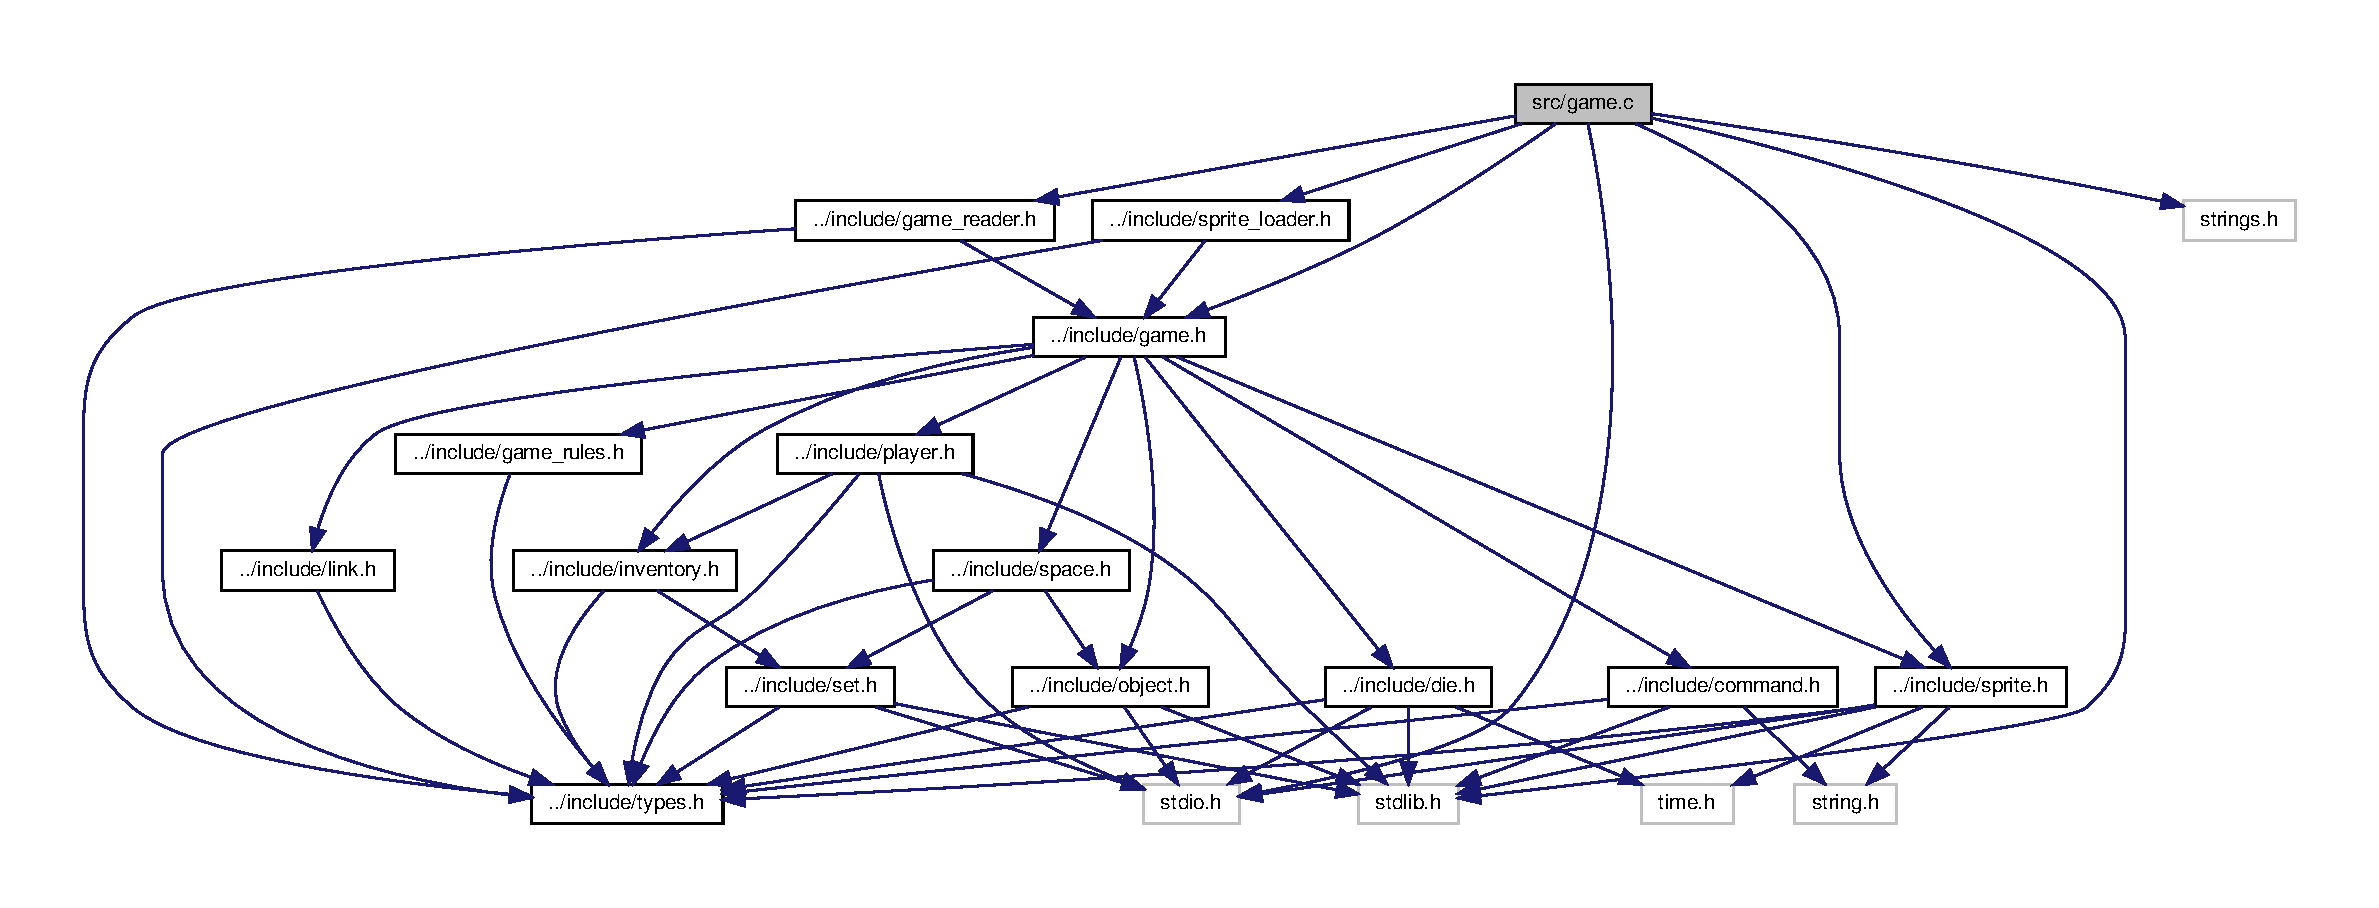
\includegraphics[width=350pt]{game_8c__incl}
\end{center}
\end{figure}
\subsection*{Classes}
\begin{DoxyCompactItemize}
\item 
struct \hyperlink{struct__Game}{\+\_\+\+Game}
\end{DoxyCompactItemize}
\subsection*{Macros}
\begin{DoxyCompactItemize}
\item 
\#define \hyperlink{game_8c_a8366e5ad74afbbea0cd0a414770c304a}{N\+\_\+\+C\+A\+L\+L\+B\+A\+CK}~11
\item 
\#define \hyperlink{game_8c_ae50e546c560a653d3409bd594d34dc0d}{P\+L\+A\+Y\+E\+R\+\_\+\+ID}~1
\item 
\#define \hyperlink{game_8c_ac4ec91c2aa48d5693e0b571427697e26}{D\+I\+E\+\_\+\+S\+E\+ED}~666
\item 
\#define \hyperlink{game_8c_ae911bb40ef7bf7ac841c05e2bfe9ff22}{S\+T\+A\+R\+T\+I\+N\+G\+\_\+\+S\+P\+A\+CE}~25
\item 
\#define \hyperlink{game_8c_ada4716d8f8fffcc46671d7adff1821ca}{N\+O\+\_\+\+L\+I\+G\+H\+T\+\_\+\+S\+P\+R\+I\+TE}~16
\end{DoxyCompactItemize}
\subsection*{Typedefs}
\begin{DoxyCompactItemize}
\item 
typedef void($\ast$ \hyperlink{game_8c_ac54a175bdefaeb274c3515fc6f43dbe5}{callback\+\_\+fn}) (\hyperlink{game_8h_a57156d39c530aec3fba3a9dad8c2dc6a}{Game} $\ast$game)
\end{DoxyCompactItemize}
\subsection*{Functions}
\begin{DoxyCompactItemize}
\item 
void \hyperlink{game_8c_ac8ed327ed13f97dcb778d0293f14d8bb}{game\+\_\+callback\+\_\+unknown} (\hyperlink{game_8h_a57156d39c530aec3fba3a9dad8c2dc6a}{Game} $\ast$game)
\item 
void \hyperlink{game_8c_acc98d79a418d2093fc3224b5c02e5418}{game\+\_\+callback\+\_\+exit} (\hyperlink{game_8h_a57156d39c530aec3fba3a9dad8c2dc6a}{Game} $\ast$game)
\item 
void \hyperlink{game_8c_a63b864e2b87c09dc2a61a55c7f26db44}{game\+\_\+callback\+\_\+pickup} (\hyperlink{game_8h_a57156d39c530aec3fba3a9dad8c2dc6a}{Game} $\ast$game)
\item 
void \hyperlink{game_8c_a424d0c659a926b0588a4287ea82552b6}{game\+\_\+callback\+\_\+drop} (\hyperlink{game_8h_a57156d39c530aec3fba3a9dad8c2dc6a}{Game} $\ast$game)
\item 
void \hyperlink{game_8c_a4929c380e741fce955cb09ad3058e6d7}{game\+\_\+callback\+\_\+roll} (\hyperlink{game_8h_a57156d39c530aec3fba3a9dad8c2dc6a}{Game} $\ast$game)
\item 
void \hyperlink{game_8c_a7525cbe807f8d1c3b698afcb75903903}{game\+\_\+callback\+\_\+move} (\hyperlink{game_8h_a57156d39c530aec3fba3a9dad8c2dc6a}{Game} $\ast$game)
\item 
void \hyperlink{game_8c_a83bb67a81f8905d8aebdc441fd23325b}{game\+\_\+callback\+\_\+check} (\hyperlink{game_8h_a57156d39c530aec3fba3a9dad8c2dc6a}{Game} $\ast$game)
\item 
void \hyperlink{game_8c_a237d569f6f570c52c2f35982c1f58ddd}{game\+\_\+callback\+\_\+turn\+On} (\hyperlink{game_8h_a57156d39c530aec3fba3a9dad8c2dc6a}{Game} $\ast$game)
\item 
void \hyperlink{game_8c_a1eabe97556a2040652c3c00254edb492}{game\+\_\+callback\+\_\+turn\+Off} (\hyperlink{game_8h_a57156d39c530aec3fba3a9dad8c2dc6a}{Game} $\ast$game)
\item 
void \hyperlink{game_8c_a22818455cb229176b145ea56485e7751}{game\+\_\+callback\+\_\+open} (\hyperlink{game_8h_a57156d39c530aec3fba3a9dad8c2dc6a}{Game} $\ast$game)
\item 
\hyperlink{game_8h_a57156d39c530aec3fba3a9dad8c2dc6a}{Game} $\ast$ \hyperlink{game_8c_a1cdbe3f06b9bf49eb5e334a22ad3b2b9}{game\+\_\+create} ()
\item 
\hyperlink{types_8h_a32c27cc471df37f4fc818d65de0a56c4}{S\+T\+A\+T\+US} \hyperlink{game_8c_afc77f90739be0fd45b7f5616e543bfae}{game\+\_\+create\+\_\+from\+\_\+file} (\hyperlink{game_8h_a57156d39c530aec3fba3a9dad8c2dc6a}{Game} $\ast$game, char $\ast$filename)
\item 
\hyperlink{types_8h_a32c27cc471df37f4fc818d65de0a56c4}{S\+T\+A\+T\+US} \hyperlink{game_8c_a0736924a1235c0e6fe9b6d91c2a12af8}{game\+\_\+destroy} (\hyperlink{game_8h_a57156d39c530aec3fba3a9dad8c2dc6a}{Game} $\ast$game)
\item 
\hyperlink{space_8h_a67533ffc2b70463baecc38fb0629bbfc}{Space} $\ast$ \hyperlink{game_8c_a69d94da9d27b542d3ebdeb8b60f1f2dc}{game\+\_\+get\+\_\+space} (\hyperlink{game_8h_a57156d39c530aec3fba3a9dad8c2dc6a}{Game} $\ast$game, \hyperlink{types_8h_a845e604fb28f7e3d97549da3448149d3}{Id} id)
\item 
\hyperlink{player_8h_af30e2030635a69690f85e48bc6ef202f}{Player} $\ast$ \hyperlink{game_8c_af46efd507d797aec6da90d08aa592e32}{game\+\_\+get\+\_\+player} (\hyperlink{game_8h_a57156d39c530aec3fba3a9dad8c2dc6a}{Game} $\ast$game)
\item 
\hyperlink{object_8h_a7f8bbcda919b65ce67f92fba08e0212f}{Object} $\ast$ \hyperlink{game_8c_a2cb6731352a9584e9d40bbb242e9a13e}{game\+\_\+get\+\_\+object} (\hyperlink{game_8h_a57156d39c530aec3fba3a9dad8c2dc6a}{Game} $\ast$game, char $\ast$object\+\_\+name)
\item 
\hyperlink{object_8h_a7f8bbcda919b65ce67f92fba08e0212f}{Object} $\ast$ \hyperlink{game_8c_a08ebb46534ea7ae3cb4708d44bdece68}{game\+\_\+get\+\_\+object\+\_\+from\+\_\+id} (\hyperlink{game_8h_a57156d39c530aec3fba3a9dad8c2dc6a}{Game} $\ast$game, \hyperlink{types_8h_a845e604fb28f7e3d97549da3448149d3}{Id} id)
\item 
\hyperlink{link_8h_ae3b299941e67be6971bfd64a25505eff}{Link} $\ast$ \hyperlink{game_8c_a1064ec927b8c33cf55982b73845db7d3}{game\+\_\+get\+\_\+link} (\hyperlink{game_8h_a57156d39c530aec3fba3a9dad8c2dc6a}{Game} $\ast$game, \hyperlink{types_8h_a845e604fb28f7e3d97549da3448149d3}{Id} id)
\item 
\hyperlink{types_8h_a845e604fb28f7e3d97549da3448149d3}{Id} \hyperlink{game_8c_af9e55e987ccd50b818c275a3dcf96527}{game\+\_\+get\+\_\+link\+\_\+id\+\_\+at} (\hyperlink{game_8h_a57156d39c530aec3fba3a9dad8c2dc6a}{Game} $\ast$game, int pos)
\item 
\hyperlink{types_8h_a845e604fb28f7e3d97549da3448149d3}{Id} \hyperlink{game_8c_ac6a628f2106f81c37d0e83c67920615f}{game\+\_\+get\+\_\+player\+\_\+location} (\hyperlink{game_8h_a57156d39c530aec3fba3a9dad8c2dc6a}{Game} $\ast$game)
\item 
\hyperlink{types_8h_a845e604fb28f7e3d97549da3448149d3}{Id} \hyperlink{game_8c_aa84eca5a1131daafd7acbf74263b6f82}{game\+\_\+get\+\_\+object\+\_\+location} (\hyperlink{game_8h_a57156d39c530aec3fba3a9dad8c2dc6a}{Game} $\ast$game, \hyperlink{types_8h_a845e604fb28f7e3d97549da3448149d3}{Id} id)
\item 
\hyperlink{types_8h_a32c27cc471df37f4fc818d65de0a56c4}{S\+T\+A\+T\+US} \hyperlink{game_8c_abdff7789be1e3a7202ac0a6a8ab7cd41}{game\+\_\+update} (\hyperlink{game_8h_a57156d39c530aec3fba3a9dad8c2dc6a}{Game} $\ast$game, \hyperlink{command_8h_a76085817cb558dc3640088040ba47898}{F\+\_\+\+Command} $\ast$cmd)
\item 
\hyperlink{command_8h_a76085817cb558dc3640088040ba47898}{F\+\_\+\+Command} $\ast$ \hyperlink{game_8c_a1ef0400a8e4f09888f01adef3b0b44d0}{game\+\_\+get\+\_\+last\+\_\+command} (\hyperlink{game_8h_a57156d39c530aec3fba3a9dad8c2dc6a}{Game} $\ast$game)
\item 
\hyperlink{command_8h_a0473597db8c45c0289b6b8e2f8abbe32}{T\+\_\+\+Command} \hyperlink{game_8c_aedbcb6a2a1b0a99505543599f040e1df}{game\+\_\+get\+\_\+last\+\_\+command\+\_\+text} (\hyperlink{game_8h_a57156d39c530aec3fba3a9dad8c2dc6a}{Game} $\ast$game)
\item 
void \hyperlink{game_8c_ab97d4976fa9cc520f216848186c0c7e0}{game\+\_\+print\+\_\+opened\+\_\+links} (\hyperlink{game_8h_a57156d39c530aec3fba3a9dad8c2dc6a}{Game} $\ast$game)
\item 
\hyperlink{types_8h_a32c27cc471df37f4fc818d65de0a56c4}{S\+T\+A\+T\+US} \hyperlink{game_8c_ae5ad86de0a92d9eccb234948458da7f1}{game\+\_\+add\+\_\+space} (\hyperlink{game_8h_a57156d39c530aec3fba3a9dad8c2dc6a}{Game} $\ast$game, \hyperlink{space_8h_a67533ffc2b70463baecc38fb0629bbfc}{Space} $\ast$space)
\item 
\hyperlink{types_8h_a32c27cc471df37f4fc818d65de0a56c4}{S\+T\+A\+T\+US} \hyperlink{game_8c_a9597a8e456aa74db536e87d56f56c3b4}{game\+\_\+add\+\_\+object} (\hyperlink{game_8h_a57156d39c530aec3fba3a9dad8c2dc6a}{Game} $\ast$game, \hyperlink{object_8h_a7f8bbcda919b65ce67f92fba08e0212f}{Object} $\ast$object)
\item 
\hyperlink{sprite_8h_a4dac9894071cab0926c0b91f2fe6e9cf}{Sprite} $\ast$ \hyperlink{game_8c_a46dafe90b177af0f04a411472893edd3}{game\+\_\+get\+\_\+sprite} (\hyperlink{game_8h_a57156d39c530aec3fba3a9dad8c2dc6a}{Game} $\ast$game, \hyperlink{types_8h_a845e604fb28f7e3d97549da3448149d3}{Id} id)
\item 
\hyperlink{types_8h_a32c27cc471df37f4fc818d65de0a56c4}{S\+T\+A\+T\+US} \hyperlink{game_8c_a6d15a79e9e897cd449f9e1c675f826d9}{game\+\_\+add\+\_\+sprite} (\hyperlink{game_8h_a57156d39c530aec3fba3a9dad8c2dc6a}{Game} $\ast$game, \hyperlink{sprite_8h_a4dac9894071cab0926c0b91f2fe6e9cf}{Sprite} $\ast$sprite, int i)
\item 
\hyperlink{types_8h_a845e604fb28f7e3d97549da3448149d3}{Id} \hyperlink{game_8c_ad2dfd865e2bd2c545a15d33f4d1cf3ae}{game\+\_\+get\+\_\+space\+\_\+id\+\_\+at} (\hyperlink{game_8h_a57156d39c530aec3fba3a9dad8c2dc6a}{Game} $\ast$game, int position)
\item 
\hyperlink{types_8h_a32c27cc471df37f4fc818d65de0a56c4}{S\+T\+A\+T\+US} \hyperlink{game_8c_a492ca9fb594442dc43fc7d18a3820426}{game\+\_\+set\+\_\+player\+\_\+location} (\hyperlink{game_8h_a57156d39c530aec3fba3a9dad8c2dc6a}{Game} $\ast$game, \hyperlink{types_8h_a845e604fb28f7e3d97549da3448149d3}{Id} id)
\item 
\hyperlink{types_8h_a32c27cc471df37f4fc818d65de0a56c4}{S\+T\+A\+T\+US} \hyperlink{game_8c_a4b9506fda0ea05cb59910e41376cbf02}{game\+\_\+set\+\_\+link} (\hyperlink{game_8h_a57156d39c530aec3fba3a9dad8c2dc6a}{Game} $\ast$game, \hyperlink{types_8h_a845e604fb28f7e3d97549da3448149d3}{Id} link\+\_\+id, \hyperlink{types_8h_a845e604fb28f7e3d97549da3448149d3}{Id} space\+\_\+id0, \hyperlink{types_8h_a845e604fb28f7e3d97549da3448149d3}{Id} space\+\_\+id1, int direction, \hyperlink{types_8h_aa60f669816b146d6373c62d9625e52ad}{Link\+Status} door)
\item 
\hyperlink{types_8h_a32c27cc471df37f4fc818d65de0a56c4}{S\+T\+A\+T\+US} \hyperlink{game_8c_a75a0a6b7a241f91e60c61ea8deb65e1d}{game\+\_\+set\+\_\+object\+\_\+location} (\hyperlink{game_8h_a57156d39c530aec3fba3a9dad8c2dc6a}{Game} $\ast$game, \hyperlink{types_8h_a845e604fb28f7e3d97549da3448149d3}{Id} id, \hyperlink{types_8h_a845e604fb28f7e3d97549da3448149d3}{Id} obj\+\_\+id, char $\ast$name, char $\ast$description)
\item 
int \hyperlink{game_8c_a58877f9f0a1d0d8d469d1aefde2c2e20}{game\+\_\+get\+\_\+last\+\_\+roll} (\hyperlink{game_8h_a57156d39c530aec3fba3a9dad8c2dc6a}{Game} $\ast$game)
\item 
\hyperlink{types_8h_a3e5b8192e7d9ffaf3542f1210aec18dd}{B\+O\+OL} \hyperlink{game_8c_af1e5cb66149225a040415851cd7ad523}{game\+\_\+are\+Spaces\+Adjacent} (\hyperlink{game_8h_a57156d39c530aec3fba3a9dad8c2dc6a}{Game} $\ast$g, \hyperlink{types_8h_a845e604fb28f7e3d97549da3448149d3}{Id} space1, \hyperlink{types_8h_a845e604fb28f7e3d97549da3448149d3}{Id} space2)
\item 
\hyperlink{types_8h_a32c27cc471df37f4fc818d65de0a56c4}{S\+T\+A\+T\+US} \hyperlink{game_8c_ad30f2b7b03d84525e33357c823b1cfdd}{update\+\_\+sprites} (\hyperlink{game_8h_a57156d39c530aec3fba3a9dad8c2dc6a}{Game} $\ast$game)
\item 
\hyperlink{types_8h_a3e5b8192e7d9ffaf3542f1210aec18dd}{B\+O\+OL} \hyperlink{game_8c_aa6efe0650af110bbd84e742cc8046d93}{game\+\_\+is\+\_\+over} (\hyperlink{game_8h_a57156d39c530aec3fba3a9dad8c2dc6a}{Game} $\ast$game)
\end{DoxyCompactItemize}
\subsection*{Variables}
\begin{DoxyCompactItemize}
\item 
static \hyperlink{game_8c_ac54a175bdefaeb274c3515fc6f43dbe5}{callback\+\_\+fn} \hyperlink{game_8c_a736ddaf27abb68c75a635760497a3f5e}{game\+\_\+callback\+\_\+fn\+\_\+list} \mbox{[}\hyperlink{game_8c_a8366e5ad74afbbea0cd0a414770c304a}{N\+\_\+\+C\+A\+L\+L\+B\+A\+CK}\mbox{]}
\end{DoxyCompactItemize}


\subsection{Detailed Description}
It implements the game interface and all the associated callbacks for each command. 

\begin{DoxyAuthor}{Author}
Profesores P\+P\+R\+OG 
\end{DoxyAuthor}
\begin{DoxyCopyright}{Copyright}
G\+NU Public License 
\end{DoxyCopyright}


\subsection{Macro Definition Documentation}
\index{game.\+c@{game.\+c}!D\+I\+E\+\_\+\+S\+E\+ED@{D\+I\+E\+\_\+\+S\+E\+ED}}
\index{D\+I\+E\+\_\+\+S\+E\+ED@{D\+I\+E\+\_\+\+S\+E\+ED}!game.\+c@{game.\+c}}
\subsubsection[{\texorpdfstring{D\+I\+E\+\_\+\+S\+E\+ED}{DIE_SEED}}]{\setlength{\rightskip}{0pt plus 5cm}\#define D\+I\+E\+\_\+\+S\+E\+ED~666}\hypertarget{game_8c_ac4ec91c2aa48d5693e0b571427697e26}{}\label{game_8c_ac4ec91c2aa48d5693e0b571427697e26}
\index{game.\+c@{game.\+c}!N\+\_\+\+C\+A\+L\+L\+B\+A\+CK@{N\+\_\+\+C\+A\+L\+L\+B\+A\+CK}}
\index{N\+\_\+\+C\+A\+L\+L\+B\+A\+CK@{N\+\_\+\+C\+A\+L\+L\+B\+A\+CK}!game.\+c@{game.\+c}}
\subsubsection[{\texorpdfstring{N\+\_\+\+C\+A\+L\+L\+B\+A\+CK}{N_CALLBACK}}]{\setlength{\rightskip}{0pt plus 5cm}\#define N\+\_\+\+C\+A\+L\+L\+B\+A\+CK~11}\hypertarget{game_8c_a8366e5ad74afbbea0cd0a414770c304a}{}\label{game_8c_a8366e5ad74afbbea0cd0a414770c304a}
\index{game.\+c@{game.\+c}!N\+O\+\_\+\+L\+I\+G\+H\+T\+\_\+\+S\+P\+R\+I\+TE@{N\+O\+\_\+\+L\+I\+G\+H\+T\+\_\+\+S\+P\+R\+I\+TE}}
\index{N\+O\+\_\+\+L\+I\+G\+H\+T\+\_\+\+S\+P\+R\+I\+TE@{N\+O\+\_\+\+L\+I\+G\+H\+T\+\_\+\+S\+P\+R\+I\+TE}!game.\+c@{game.\+c}}
\subsubsection[{\texorpdfstring{N\+O\+\_\+\+L\+I\+G\+H\+T\+\_\+\+S\+P\+R\+I\+TE}{NO_LIGHT_SPRITE}}]{\setlength{\rightskip}{0pt plus 5cm}\#define N\+O\+\_\+\+L\+I\+G\+H\+T\+\_\+\+S\+P\+R\+I\+TE~16}\hypertarget{game_8c_ada4716d8f8fffcc46671d7adff1821ca}{}\label{game_8c_ada4716d8f8fffcc46671d7adff1821ca}
\index{game.\+c@{game.\+c}!P\+L\+A\+Y\+E\+R\+\_\+\+ID@{P\+L\+A\+Y\+E\+R\+\_\+\+ID}}
\index{P\+L\+A\+Y\+E\+R\+\_\+\+ID@{P\+L\+A\+Y\+E\+R\+\_\+\+ID}!game.\+c@{game.\+c}}
\subsubsection[{\texorpdfstring{P\+L\+A\+Y\+E\+R\+\_\+\+ID}{PLAYER_ID}}]{\setlength{\rightskip}{0pt plus 5cm}\#define P\+L\+A\+Y\+E\+R\+\_\+\+ID~1}\hypertarget{game_8c_ae50e546c560a653d3409bd594d34dc0d}{}\label{game_8c_ae50e546c560a653d3409bd594d34dc0d}
\index{game.\+c@{game.\+c}!S\+T\+A\+R\+T\+I\+N\+G\+\_\+\+S\+P\+A\+CE@{S\+T\+A\+R\+T\+I\+N\+G\+\_\+\+S\+P\+A\+CE}}
\index{S\+T\+A\+R\+T\+I\+N\+G\+\_\+\+S\+P\+A\+CE@{S\+T\+A\+R\+T\+I\+N\+G\+\_\+\+S\+P\+A\+CE}!game.\+c@{game.\+c}}
\subsubsection[{\texorpdfstring{S\+T\+A\+R\+T\+I\+N\+G\+\_\+\+S\+P\+A\+CE}{STARTING_SPACE}}]{\setlength{\rightskip}{0pt plus 5cm}\#define S\+T\+A\+R\+T\+I\+N\+G\+\_\+\+S\+P\+A\+CE~25}\hypertarget{game_8c_ae911bb40ef7bf7ac841c05e2bfe9ff22}{}\label{game_8c_ae911bb40ef7bf7ac841c05e2bfe9ff22}


\subsection{Typedef Documentation}
\index{game.\+c@{game.\+c}!callback\+\_\+fn@{callback\+\_\+fn}}
\index{callback\+\_\+fn@{callback\+\_\+fn}!game.\+c@{game.\+c}}
\subsubsection[{\texorpdfstring{callback\+\_\+fn}{callback_fn}}]{\setlength{\rightskip}{0pt plus 5cm}typedef void($\ast$ callback\+\_\+fn) ({\bf Game} $\ast$game)}\hypertarget{game_8c_ac54a175bdefaeb274c3515fc6f43dbe5}{}\label{game_8c_ac54a175bdefaeb274c3515fc6f43dbe5}
Define the function type for the callbacks 

\subsection{Function Documentation}
\index{game.\+c@{game.\+c}!game\+\_\+add\+\_\+object@{game\+\_\+add\+\_\+object}}
\index{game\+\_\+add\+\_\+object@{game\+\_\+add\+\_\+object}!game.\+c@{game.\+c}}
\subsubsection[{\texorpdfstring{game\+\_\+add\+\_\+object(\+Game $\ast$game, Object $\ast$object)}{game_add_object(Game *game, Object *object)}}]{\setlength{\rightskip}{0pt plus 5cm}{\bf S\+T\+A\+T\+US} game\+\_\+add\+\_\+object (
\begin{DoxyParamCaption}
\item[{{\bf Game} $\ast$}]{game, }
\item[{{\bf Object} $\ast$}]{object}
\end{DoxyParamCaption}
)}\hypertarget{game_8c_a9597a8e456aa74db536e87d56f56c3b4}{}\label{game_8c_a9597a8e456aa74db536e87d56f56c3b4}
\index{game.\+c@{game.\+c}!game\+\_\+add\+\_\+space@{game\+\_\+add\+\_\+space}}
\index{game\+\_\+add\+\_\+space@{game\+\_\+add\+\_\+space}!game.\+c@{game.\+c}}
\subsubsection[{\texorpdfstring{game\+\_\+add\+\_\+space(\+Game $\ast$game, Space $\ast$space)}{game_add_space(Game *game, Space *space)}}]{\setlength{\rightskip}{0pt plus 5cm}{\bf S\+T\+A\+T\+US} game\+\_\+add\+\_\+space (
\begin{DoxyParamCaption}
\item[{{\bf Game} $\ast$}]{game, }
\item[{{\bf Space} $\ast$}]{space}
\end{DoxyParamCaption}
)}\hypertarget{game_8c_ae5ad86de0a92d9eccb234948458da7f1}{}\label{game_8c_ae5ad86de0a92d9eccb234948458da7f1}
\index{game.\+c@{game.\+c}!game\+\_\+add\+\_\+sprite@{game\+\_\+add\+\_\+sprite}}
\index{game\+\_\+add\+\_\+sprite@{game\+\_\+add\+\_\+sprite}!game.\+c@{game.\+c}}
\subsubsection[{\texorpdfstring{game\+\_\+add\+\_\+sprite(\+Game $\ast$game, Sprite $\ast$sprite, int i)}{game_add_sprite(Game *game, Sprite *sprite, int i)}}]{\setlength{\rightskip}{0pt plus 5cm}{\bf S\+T\+A\+T\+US} game\+\_\+add\+\_\+sprite (
\begin{DoxyParamCaption}
\item[{{\bf Game} $\ast$}]{game, }
\item[{{\bf Sprite} $\ast$}]{sprite, }
\item[{int}]{i}
\end{DoxyParamCaption}
)}\hypertarget{game_8c_a6d15a79e9e897cd449f9e1c675f826d9}{}\label{game_8c_a6d15a79e9e897cd449f9e1c675f826d9}
\index{game.\+c@{game.\+c}!game\+\_\+are\+Spaces\+Adjacent@{game\+\_\+are\+Spaces\+Adjacent}}
\index{game\+\_\+are\+Spaces\+Adjacent@{game\+\_\+are\+Spaces\+Adjacent}!game.\+c@{game.\+c}}
\subsubsection[{\texorpdfstring{game\+\_\+are\+Spaces\+Adjacent(\+Game $\ast$g, Id space1, Id space2)}{game_areSpacesAdjacent(Game *g, Id space1, Id space2)}}]{\setlength{\rightskip}{0pt plus 5cm}{\bf B\+O\+OL} game\+\_\+are\+Spaces\+Adjacent (
\begin{DoxyParamCaption}
\item[{{\bf Game} $\ast$}]{g, }
\item[{{\bf Id}}]{space1, }
\item[{{\bf Id}}]{space2}
\end{DoxyParamCaption}
)}\hypertarget{game_8c_af1e5cb66149225a040415851cd7ad523}{}\label{game_8c_af1e5cb66149225a040415851cd7ad523}
\index{game.\+c@{game.\+c}!game\+\_\+callback\+\_\+check@{game\+\_\+callback\+\_\+check}}
\index{game\+\_\+callback\+\_\+check@{game\+\_\+callback\+\_\+check}!game.\+c@{game.\+c}}
\subsubsection[{\texorpdfstring{game\+\_\+callback\+\_\+check(\+Game $\ast$game)}{game_callback_check(Game *game)}}]{\setlength{\rightskip}{0pt plus 5cm}void game\+\_\+callback\+\_\+check (
\begin{DoxyParamCaption}
\item[{{\bf Game} $\ast$}]{game}
\end{DoxyParamCaption}
)}\hypertarget{game_8c_a83bb67a81f8905d8aebdc441fd23325b}{}\label{game_8c_a83bb67a81f8905d8aebdc441fd23325b}
\index{game.\+c@{game.\+c}!game\+\_\+callback\+\_\+drop@{game\+\_\+callback\+\_\+drop}}
\index{game\+\_\+callback\+\_\+drop@{game\+\_\+callback\+\_\+drop}!game.\+c@{game.\+c}}
\subsubsection[{\texorpdfstring{game\+\_\+callback\+\_\+drop(\+Game $\ast$game)}{game_callback_drop(Game *game)}}]{\setlength{\rightskip}{0pt plus 5cm}void game\+\_\+callback\+\_\+drop (
\begin{DoxyParamCaption}
\item[{{\bf Game} $\ast$}]{game}
\end{DoxyParamCaption}
)}\hypertarget{game_8c_a424d0c659a926b0588a4287ea82552b6}{}\label{game_8c_a424d0c659a926b0588a4287ea82552b6}
\index{game.\+c@{game.\+c}!game\+\_\+callback\+\_\+exit@{game\+\_\+callback\+\_\+exit}}
\index{game\+\_\+callback\+\_\+exit@{game\+\_\+callback\+\_\+exit}!game.\+c@{game.\+c}}
\subsubsection[{\texorpdfstring{game\+\_\+callback\+\_\+exit(\+Game $\ast$game)}{game_callback_exit(Game *game)}}]{\setlength{\rightskip}{0pt plus 5cm}void game\+\_\+callback\+\_\+exit (
\begin{DoxyParamCaption}
\item[{{\bf Game} $\ast$}]{game}
\end{DoxyParamCaption}
)}\hypertarget{game_8c_acc98d79a418d2093fc3224b5c02e5418}{}\label{game_8c_acc98d79a418d2093fc3224b5c02e5418}
\index{game.\+c@{game.\+c}!game\+\_\+callback\+\_\+move@{game\+\_\+callback\+\_\+move}}
\index{game\+\_\+callback\+\_\+move@{game\+\_\+callback\+\_\+move}!game.\+c@{game.\+c}}
\subsubsection[{\texorpdfstring{game\+\_\+callback\+\_\+move(\+Game $\ast$game)}{game_callback_move(Game *game)}}]{\setlength{\rightskip}{0pt plus 5cm}void game\+\_\+callback\+\_\+move (
\begin{DoxyParamCaption}
\item[{{\bf Game} $\ast$}]{game}
\end{DoxyParamCaption}
)}\hypertarget{game_8c_a7525cbe807f8d1c3b698afcb75903903}{}\label{game_8c_a7525cbe807f8d1c3b698afcb75903903}
\index{game.\+c@{game.\+c}!game\+\_\+callback\+\_\+open@{game\+\_\+callback\+\_\+open}}
\index{game\+\_\+callback\+\_\+open@{game\+\_\+callback\+\_\+open}!game.\+c@{game.\+c}}
\subsubsection[{\texorpdfstring{game\+\_\+callback\+\_\+open(\+Game $\ast$game)}{game_callback_open(Game *game)}}]{\setlength{\rightskip}{0pt plus 5cm}void game\+\_\+callback\+\_\+open (
\begin{DoxyParamCaption}
\item[{{\bf Game} $\ast$}]{game}
\end{DoxyParamCaption}
)}\hypertarget{game_8c_a22818455cb229176b145ea56485e7751}{}\label{game_8c_a22818455cb229176b145ea56485e7751}
\index{game.\+c@{game.\+c}!game\+\_\+callback\+\_\+pickup@{game\+\_\+callback\+\_\+pickup}}
\index{game\+\_\+callback\+\_\+pickup@{game\+\_\+callback\+\_\+pickup}!game.\+c@{game.\+c}}
\subsubsection[{\texorpdfstring{game\+\_\+callback\+\_\+pickup(\+Game $\ast$game)}{game_callback_pickup(Game *game)}}]{\setlength{\rightskip}{0pt plus 5cm}void game\+\_\+callback\+\_\+pickup (
\begin{DoxyParamCaption}
\item[{{\bf Game} $\ast$}]{game}
\end{DoxyParamCaption}
)}\hypertarget{game_8c_a63b864e2b87c09dc2a61a55c7f26db44}{}\label{game_8c_a63b864e2b87c09dc2a61a55c7f26db44}
\index{game.\+c@{game.\+c}!game\+\_\+callback\+\_\+roll@{game\+\_\+callback\+\_\+roll}}
\index{game\+\_\+callback\+\_\+roll@{game\+\_\+callback\+\_\+roll}!game.\+c@{game.\+c}}
\subsubsection[{\texorpdfstring{game\+\_\+callback\+\_\+roll(\+Game $\ast$game)}{game_callback_roll(Game *game)}}]{\setlength{\rightskip}{0pt plus 5cm}void game\+\_\+callback\+\_\+roll (
\begin{DoxyParamCaption}
\item[{{\bf Game} $\ast$}]{game}
\end{DoxyParamCaption}
)}\hypertarget{game_8c_a4929c380e741fce955cb09ad3058e6d7}{}\label{game_8c_a4929c380e741fce955cb09ad3058e6d7}
\index{game.\+c@{game.\+c}!game\+\_\+callback\+\_\+turn\+Off@{game\+\_\+callback\+\_\+turn\+Off}}
\index{game\+\_\+callback\+\_\+turn\+Off@{game\+\_\+callback\+\_\+turn\+Off}!game.\+c@{game.\+c}}
\subsubsection[{\texorpdfstring{game\+\_\+callback\+\_\+turn\+Off(\+Game $\ast$game)}{game_callback_turnOff(Game *game)}}]{\setlength{\rightskip}{0pt plus 5cm}void game\+\_\+callback\+\_\+turn\+Off (
\begin{DoxyParamCaption}
\item[{{\bf Game} $\ast$}]{game}
\end{DoxyParamCaption}
)}\hypertarget{game_8c_a1eabe97556a2040652c3c00254edb492}{}\label{game_8c_a1eabe97556a2040652c3c00254edb492}
\index{game.\+c@{game.\+c}!game\+\_\+callback\+\_\+turn\+On@{game\+\_\+callback\+\_\+turn\+On}}
\index{game\+\_\+callback\+\_\+turn\+On@{game\+\_\+callback\+\_\+turn\+On}!game.\+c@{game.\+c}}
\subsubsection[{\texorpdfstring{game\+\_\+callback\+\_\+turn\+On(\+Game $\ast$game)}{game_callback_turnOn(Game *game)}}]{\setlength{\rightskip}{0pt plus 5cm}void game\+\_\+callback\+\_\+turn\+On (
\begin{DoxyParamCaption}
\item[{{\bf Game} $\ast$}]{game}
\end{DoxyParamCaption}
)}\hypertarget{game_8c_a237d569f6f570c52c2f35982c1f58ddd}{}\label{game_8c_a237d569f6f570c52c2f35982c1f58ddd}
\index{game.\+c@{game.\+c}!game\+\_\+callback\+\_\+unknown@{game\+\_\+callback\+\_\+unknown}}
\index{game\+\_\+callback\+\_\+unknown@{game\+\_\+callback\+\_\+unknown}!game.\+c@{game.\+c}}
\subsubsection[{\texorpdfstring{game\+\_\+callback\+\_\+unknown(\+Game $\ast$game)}{game_callback_unknown(Game *game)}}]{\setlength{\rightskip}{0pt plus 5cm}void game\+\_\+callback\+\_\+unknown (
\begin{DoxyParamCaption}
\item[{{\bf Game} $\ast$}]{game}
\end{DoxyParamCaption}
)}\hypertarget{game_8c_ac8ed327ed13f97dcb778d0293f14d8bb}{}\label{game_8c_ac8ed327ed13f97dcb778d0293f14d8bb}
List of callbacks for each command in the game \index{game.\+c@{game.\+c}!game\+\_\+create@{game\+\_\+create}}
\index{game\+\_\+create@{game\+\_\+create}!game.\+c@{game.\+c}}
\subsubsection[{\texorpdfstring{game\+\_\+create()}{game_create()}}]{\setlength{\rightskip}{0pt plus 5cm}{\bf Game}$\ast$ game\+\_\+create (
\begin{DoxyParamCaption}
{}
\end{DoxyParamCaption}
)}\hypertarget{game_8c_a1cdbe3f06b9bf49eb5e334a22ad3b2b9}{}\label{game_8c_a1cdbe3f06b9bf49eb5e334a22ad3b2b9}
\index{game.\+c@{game.\+c}!game\+\_\+create\+\_\+from\+\_\+file@{game\+\_\+create\+\_\+from\+\_\+file}}
\index{game\+\_\+create\+\_\+from\+\_\+file@{game\+\_\+create\+\_\+from\+\_\+file}!game.\+c@{game.\+c}}
\subsubsection[{\texorpdfstring{game\+\_\+create\+\_\+from\+\_\+file(\+Game $\ast$game, char $\ast$filename)}{game_create_from_file(Game *game, char *filename)}}]{\setlength{\rightskip}{0pt plus 5cm}{\bf S\+T\+A\+T\+US} game\+\_\+create\+\_\+from\+\_\+file (
\begin{DoxyParamCaption}
\item[{{\bf Game} $\ast$}]{game, }
\item[{char $\ast$}]{filename}
\end{DoxyParamCaption}
)}\hypertarget{game_8c_afc77f90739be0fd45b7f5616e543bfae}{}\label{game_8c_afc77f90739be0fd45b7f5616e543bfae}
\index{game.\+c@{game.\+c}!game\+\_\+destroy@{game\+\_\+destroy}}
\index{game\+\_\+destroy@{game\+\_\+destroy}!game.\+c@{game.\+c}}
\subsubsection[{\texorpdfstring{game\+\_\+destroy(\+Game $\ast$game)}{game_destroy(Game *game)}}]{\setlength{\rightskip}{0pt plus 5cm}{\bf S\+T\+A\+T\+US} game\+\_\+destroy (
\begin{DoxyParamCaption}
\item[{{\bf Game} $\ast$}]{game}
\end{DoxyParamCaption}
)}\hypertarget{game_8c_a0736924a1235c0e6fe9b6d91c2a12af8}{}\label{game_8c_a0736924a1235c0e6fe9b6d91c2a12af8}
\index{game.\+c@{game.\+c}!game\+\_\+get\+\_\+last\+\_\+command@{game\+\_\+get\+\_\+last\+\_\+command}}
\index{game\+\_\+get\+\_\+last\+\_\+command@{game\+\_\+get\+\_\+last\+\_\+command}!game.\+c@{game.\+c}}
\subsubsection[{\texorpdfstring{game\+\_\+get\+\_\+last\+\_\+command(\+Game $\ast$game)}{game_get_last_command(Game *game)}}]{\setlength{\rightskip}{0pt plus 5cm}{\bf F\+\_\+\+Command}$\ast$ game\+\_\+get\+\_\+last\+\_\+command (
\begin{DoxyParamCaption}
\item[{{\bf Game} $\ast$}]{game}
\end{DoxyParamCaption}
)}\hypertarget{game_8c_a1ef0400a8e4f09888f01adef3b0b44d0}{}\label{game_8c_a1ef0400a8e4f09888f01adef3b0b44d0}
\index{game.\+c@{game.\+c}!game\+\_\+get\+\_\+last\+\_\+command\+\_\+text@{game\+\_\+get\+\_\+last\+\_\+command\+\_\+text}}
\index{game\+\_\+get\+\_\+last\+\_\+command\+\_\+text@{game\+\_\+get\+\_\+last\+\_\+command\+\_\+text}!game.\+c@{game.\+c}}
\subsubsection[{\texorpdfstring{game\+\_\+get\+\_\+last\+\_\+command\+\_\+text(\+Game $\ast$game)}{game_get_last_command_text(Game *game)}}]{\setlength{\rightskip}{0pt plus 5cm}{\bf T\+\_\+\+Command} game\+\_\+get\+\_\+last\+\_\+command\+\_\+text (
\begin{DoxyParamCaption}
\item[{{\bf Game} $\ast$}]{game}
\end{DoxyParamCaption}
)}\hypertarget{game_8c_aedbcb6a2a1b0a99505543599f040e1df}{}\label{game_8c_aedbcb6a2a1b0a99505543599f040e1df}
\index{game.\+c@{game.\+c}!game\+\_\+get\+\_\+last\+\_\+roll@{game\+\_\+get\+\_\+last\+\_\+roll}}
\index{game\+\_\+get\+\_\+last\+\_\+roll@{game\+\_\+get\+\_\+last\+\_\+roll}!game.\+c@{game.\+c}}
\subsubsection[{\texorpdfstring{game\+\_\+get\+\_\+last\+\_\+roll(\+Game $\ast$game)}{game_get_last_roll(Game *game)}}]{\setlength{\rightskip}{0pt plus 5cm}int game\+\_\+get\+\_\+last\+\_\+roll (
\begin{DoxyParamCaption}
\item[{{\bf Game} $\ast$}]{game}
\end{DoxyParamCaption}
)}\hypertarget{game_8c_a58877f9f0a1d0d8d469d1aefde2c2e20}{}\label{game_8c_a58877f9f0a1d0d8d469d1aefde2c2e20}
\index{game.\+c@{game.\+c}!game\+\_\+get\+\_\+link@{game\+\_\+get\+\_\+link}}
\index{game\+\_\+get\+\_\+link@{game\+\_\+get\+\_\+link}!game.\+c@{game.\+c}}
\subsubsection[{\texorpdfstring{game\+\_\+get\+\_\+link(\+Game $\ast$game, Id id)}{game_get_link(Game *game, Id id)}}]{\setlength{\rightskip}{0pt plus 5cm}{\bf Link}$\ast$ game\+\_\+get\+\_\+link (
\begin{DoxyParamCaption}
\item[{{\bf Game} $\ast$}]{game, }
\item[{{\bf Id}}]{id}
\end{DoxyParamCaption}
)}\hypertarget{game_8c_a1064ec927b8c33cf55982b73845db7d3}{}\label{game_8c_a1064ec927b8c33cf55982b73845db7d3}
\index{game.\+c@{game.\+c}!game\+\_\+get\+\_\+link\+\_\+id\+\_\+at@{game\+\_\+get\+\_\+link\+\_\+id\+\_\+at}}
\index{game\+\_\+get\+\_\+link\+\_\+id\+\_\+at@{game\+\_\+get\+\_\+link\+\_\+id\+\_\+at}!game.\+c@{game.\+c}}
\subsubsection[{\texorpdfstring{game\+\_\+get\+\_\+link\+\_\+id\+\_\+at(\+Game $\ast$game, int pos)}{game_get_link_id_at(Game *game, int pos)}}]{\setlength{\rightskip}{0pt plus 5cm}{\bf Id} game\+\_\+get\+\_\+link\+\_\+id\+\_\+at (
\begin{DoxyParamCaption}
\item[{{\bf Game} $\ast$}]{game, }
\item[{int}]{pos}
\end{DoxyParamCaption}
)}\hypertarget{game_8c_af9e55e987ccd50b818c275a3dcf96527}{}\label{game_8c_af9e55e987ccd50b818c275a3dcf96527}
\index{game.\+c@{game.\+c}!game\+\_\+get\+\_\+object@{game\+\_\+get\+\_\+object}}
\index{game\+\_\+get\+\_\+object@{game\+\_\+get\+\_\+object}!game.\+c@{game.\+c}}
\subsubsection[{\texorpdfstring{game\+\_\+get\+\_\+object(\+Game $\ast$game, char $\ast$object\+\_\+name)}{game_get_object(Game *game, char *object_name)}}]{\setlength{\rightskip}{0pt plus 5cm}{\bf Object}$\ast$ game\+\_\+get\+\_\+object (
\begin{DoxyParamCaption}
\item[{{\bf Game} $\ast$}]{game, }
\item[{char $\ast$}]{object\+\_\+name}
\end{DoxyParamCaption}
)}\hypertarget{game_8c_a2cb6731352a9584e9d40bbb242e9a13e}{}\label{game_8c_a2cb6731352a9584e9d40bbb242e9a13e}
\index{game.\+c@{game.\+c}!game\+\_\+get\+\_\+object\+\_\+from\+\_\+id@{game\+\_\+get\+\_\+object\+\_\+from\+\_\+id}}
\index{game\+\_\+get\+\_\+object\+\_\+from\+\_\+id@{game\+\_\+get\+\_\+object\+\_\+from\+\_\+id}!game.\+c@{game.\+c}}
\subsubsection[{\texorpdfstring{game\+\_\+get\+\_\+object\+\_\+from\+\_\+id(\+Game $\ast$game, Id id)}{game_get_object_from_id(Game *game, Id id)}}]{\setlength{\rightskip}{0pt plus 5cm}{\bf Object}$\ast$ game\+\_\+get\+\_\+object\+\_\+from\+\_\+id (
\begin{DoxyParamCaption}
\item[{{\bf Game} $\ast$}]{game, }
\item[{{\bf Id}}]{id}
\end{DoxyParamCaption}
)}\hypertarget{game_8c_a08ebb46534ea7ae3cb4708d44bdece68}{}\label{game_8c_a08ebb46534ea7ae3cb4708d44bdece68}
\index{game.\+c@{game.\+c}!game\+\_\+get\+\_\+object\+\_\+location@{game\+\_\+get\+\_\+object\+\_\+location}}
\index{game\+\_\+get\+\_\+object\+\_\+location@{game\+\_\+get\+\_\+object\+\_\+location}!game.\+c@{game.\+c}}
\subsubsection[{\texorpdfstring{game\+\_\+get\+\_\+object\+\_\+location(\+Game $\ast$game, Id id)}{game_get_object_location(Game *game, Id id)}}]{\setlength{\rightskip}{0pt plus 5cm}{\bf Id} game\+\_\+get\+\_\+object\+\_\+location (
\begin{DoxyParamCaption}
\item[{{\bf Game} $\ast$}]{game, }
\item[{{\bf Id}}]{id}
\end{DoxyParamCaption}
)}\hypertarget{game_8c_aa84eca5a1131daafd7acbf74263b6f82}{}\label{game_8c_aa84eca5a1131daafd7acbf74263b6f82}
\index{game.\+c@{game.\+c}!game\+\_\+get\+\_\+player@{game\+\_\+get\+\_\+player}}
\index{game\+\_\+get\+\_\+player@{game\+\_\+get\+\_\+player}!game.\+c@{game.\+c}}
\subsubsection[{\texorpdfstring{game\+\_\+get\+\_\+player(\+Game $\ast$game)}{game_get_player(Game *game)}}]{\setlength{\rightskip}{0pt plus 5cm}{\bf Player}$\ast$ game\+\_\+get\+\_\+player (
\begin{DoxyParamCaption}
\item[{{\bf Game} $\ast$}]{game}
\end{DoxyParamCaption}
)}\hypertarget{game_8c_af46efd507d797aec6da90d08aa592e32}{}\label{game_8c_af46efd507d797aec6da90d08aa592e32}
\index{game.\+c@{game.\+c}!game\+\_\+get\+\_\+player\+\_\+location@{game\+\_\+get\+\_\+player\+\_\+location}}
\index{game\+\_\+get\+\_\+player\+\_\+location@{game\+\_\+get\+\_\+player\+\_\+location}!game.\+c@{game.\+c}}
\subsubsection[{\texorpdfstring{game\+\_\+get\+\_\+player\+\_\+location(\+Game $\ast$game)}{game_get_player_location(Game *game)}}]{\setlength{\rightskip}{0pt plus 5cm}{\bf Id} game\+\_\+get\+\_\+player\+\_\+location (
\begin{DoxyParamCaption}
\item[{{\bf Game} $\ast$}]{game}
\end{DoxyParamCaption}
)}\hypertarget{game_8c_ac6a628f2106f81c37d0e83c67920615f}{}\label{game_8c_ac6a628f2106f81c37d0e83c67920615f}
\index{game.\+c@{game.\+c}!game\+\_\+get\+\_\+space@{game\+\_\+get\+\_\+space}}
\index{game\+\_\+get\+\_\+space@{game\+\_\+get\+\_\+space}!game.\+c@{game.\+c}}
\subsubsection[{\texorpdfstring{game\+\_\+get\+\_\+space(\+Game $\ast$game, Id id)}{game_get_space(Game *game, Id id)}}]{\setlength{\rightskip}{0pt plus 5cm}{\bf Space}$\ast$ game\+\_\+get\+\_\+space (
\begin{DoxyParamCaption}
\item[{{\bf Game} $\ast$}]{game, }
\item[{{\bf Id}}]{id}
\end{DoxyParamCaption}
)}\hypertarget{game_8c_a69d94da9d27b542d3ebdeb8b60f1f2dc}{}\label{game_8c_a69d94da9d27b542d3ebdeb8b60f1f2dc}
\index{game.\+c@{game.\+c}!game\+\_\+get\+\_\+space\+\_\+id\+\_\+at@{game\+\_\+get\+\_\+space\+\_\+id\+\_\+at}}
\index{game\+\_\+get\+\_\+space\+\_\+id\+\_\+at@{game\+\_\+get\+\_\+space\+\_\+id\+\_\+at}!game.\+c@{game.\+c}}
\subsubsection[{\texorpdfstring{game\+\_\+get\+\_\+space\+\_\+id\+\_\+at(\+Game $\ast$game, int position)}{game_get_space_id_at(Game *game, int position)}}]{\setlength{\rightskip}{0pt plus 5cm}{\bf Id} game\+\_\+get\+\_\+space\+\_\+id\+\_\+at (
\begin{DoxyParamCaption}
\item[{{\bf Game} $\ast$}]{game, }
\item[{int}]{position}
\end{DoxyParamCaption}
)}\hypertarget{game_8c_ad2dfd865e2bd2c545a15d33f4d1cf3ae}{}\label{game_8c_ad2dfd865e2bd2c545a15d33f4d1cf3ae}
\index{game.\+c@{game.\+c}!game\+\_\+get\+\_\+sprite@{game\+\_\+get\+\_\+sprite}}
\index{game\+\_\+get\+\_\+sprite@{game\+\_\+get\+\_\+sprite}!game.\+c@{game.\+c}}
\subsubsection[{\texorpdfstring{game\+\_\+get\+\_\+sprite(\+Game $\ast$game, Id id)}{game_get_sprite(Game *game, Id id)}}]{\setlength{\rightskip}{0pt plus 5cm}{\bf Sprite}$\ast$ game\+\_\+get\+\_\+sprite (
\begin{DoxyParamCaption}
\item[{{\bf Game} $\ast$}]{game, }
\item[{{\bf Id}}]{id}
\end{DoxyParamCaption}
)}\hypertarget{game_8c_a46dafe90b177af0f04a411472893edd3}{}\label{game_8c_a46dafe90b177af0f04a411472893edd3}
\index{game.\+c@{game.\+c}!game\+\_\+is\+\_\+over@{game\+\_\+is\+\_\+over}}
\index{game\+\_\+is\+\_\+over@{game\+\_\+is\+\_\+over}!game.\+c@{game.\+c}}
\subsubsection[{\texorpdfstring{game\+\_\+is\+\_\+over(\+Game $\ast$game)}{game_is_over(Game *game)}}]{\setlength{\rightskip}{0pt plus 5cm}{\bf B\+O\+OL} game\+\_\+is\+\_\+over (
\begin{DoxyParamCaption}
\item[{{\bf Game} $\ast$}]{game}
\end{DoxyParamCaption}
)}\hypertarget{game_8c_aa6efe0650af110bbd84e742cc8046d93}{}\label{game_8c_aa6efe0650af110bbd84e742cc8046d93}
\index{game.\+c@{game.\+c}!game\+\_\+print\+\_\+opened\+\_\+links@{game\+\_\+print\+\_\+opened\+\_\+links}}
\index{game\+\_\+print\+\_\+opened\+\_\+links@{game\+\_\+print\+\_\+opened\+\_\+links}!game.\+c@{game.\+c}}
\subsubsection[{\texorpdfstring{game\+\_\+print\+\_\+opened\+\_\+links(\+Game $\ast$game)}{game_print_opened_links(Game *game)}}]{\setlength{\rightskip}{0pt plus 5cm}void game\+\_\+print\+\_\+opened\+\_\+links (
\begin{DoxyParamCaption}
\item[{{\bf Game} $\ast$}]{game}
\end{DoxyParamCaption}
)}\hypertarget{game_8c_ab97d4976fa9cc520f216848186c0c7e0}{}\label{game_8c_ab97d4976fa9cc520f216848186c0c7e0}
\index{game.\+c@{game.\+c}!game\+\_\+set\+\_\+link@{game\+\_\+set\+\_\+link}}
\index{game\+\_\+set\+\_\+link@{game\+\_\+set\+\_\+link}!game.\+c@{game.\+c}}
\subsubsection[{\texorpdfstring{game\+\_\+set\+\_\+link(\+Game $\ast$game, Id link\+\_\+id, Id space\+\_\+id0, Id space\+\_\+id1, int direction, Link\+Status door)}{game_set_link(Game *game, Id link_id, Id space_id0, Id space_id1, int direction, LinkStatus door)}}]{\setlength{\rightskip}{0pt plus 5cm}{\bf S\+T\+A\+T\+US} game\+\_\+set\+\_\+link (
\begin{DoxyParamCaption}
\item[{{\bf Game} $\ast$}]{game, }
\item[{{\bf Id}}]{link\+\_\+id, }
\item[{{\bf Id}}]{space\+\_\+id0, }
\item[{{\bf Id}}]{space\+\_\+id1, }
\item[{int}]{direction, }
\item[{{\bf Link\+Status}}]{door}
\end{DoxyParamCaption}
)}\hypertarget{game_8c_a4b9506fda0ea05cb59910e41376cbf02}{}\label{game_8c_a4b9506fda0ea05cb59910e41376cbf02}
\index{game.\+c@{game.\+c}!game\+\_\+set\+\_\+object\+\_\+location@{game\+\_\+set\+\_\+object\+\_\+location}}
\index{game\+\_\+set\+\_\+object\+\_\+location@{game\+\_\+set\+\_\+object\+\_\+location}!game.\+c@{game.\+c}}
\subsubsection[{\texorpdfstring{game\+\_\+set\+\_\+object\+\_\+location(\+Game $\ast$game, Id id, Id obj\+\_\+id, char $\ast$name, char $\ast$description)}{game_set_object_location(Game *game, Id id, Id obj_id, char *name, char *description)}}]{\setlength{\rightskip}{0pt plus 5cm}{\bf S\+T\+A\+T\+US} game\+\_\+set\+\_\+object\+\_\+location (
\begin{DoxyParamCaption}
\item[{{\bf Game} $\ast$}]{game, }
\item[{{\bf Id}}]{id, }
\item[{{\bf Id}}]{obj\+\_\+id, }
\item[{char $\ast$}]{name, }
\item[{char $\ast$}]{description}
\end{DoxyParamCaption}
)}\hypertarget{game_8c_a75a0a6b7a241f91e60c61ea8deb65e1d}{}\label{game_8c_a75a0a6b7a241f91e60c61ea8deb65e1d}
\index{game.\+c@{game.\+c}!game\+\_\+set\+\_\+player\+\_\+location@{game\+\_\+set\+\_\+player\+\_\+location}}
\index{game\+\_\+set\+\_\+player\+\_\+location@{game\+\_\+set\+\_\+player\+\_\+location}!game.\+c@{game.\+c}}
\subsubsection[{\texorpdfstring{game\+\_\+set\+\_\+player\+\_\+location(\+Game $\ast$game, Id id)}{game_set_player_location(Game *game, Id id)}}]{\setlength{\rightskip}{0pt plus 5cm}{\bf S\+T\+A\+T\+US} game\+\_\+set\+\_\+player\+\_\+location (
\begin{DoxyParamCaption}
\item[{{\bf Game} $\ast$}]{game, }
\item[{{\bf Id}}]{id}
\end{DoxyParamCaption}
)}\hypertarget{game_8c_a492ca9fb594442dc43fc7d18a3820426}{}\label{game_8c_a492ca9fb594442dc43fc7d18a3820426}
\index{game.\+c@{game.\+c}!game\+\_\+update@{game\+\_\+update}}
\index{game\+\_\+update@{game\+\_\+update}!game.\+c@{game.\+c}}
\subsubsection[{\texorpdfstring{game\+\_\+update(\+Game $\ast$game, F\+\_\+\+Command $\ast$cmd)}{game_update(Game *game, F_Command *cmd)}}]{\setlength{\rightskip}{0pt plus 5cm}{\bf S\+T\+A\+T\+US} game\+\_\+update (
\begin{DoxyParamCaption}
\item[{{\bf Game} $\ast$}]{game, }
\item[{{\bf F\+\_\+\+Command} $\ast$}]{cmd}
\end{DoxyParamCaption}
)}\hypertarget{game_8c_abdff7789be1e3a7202ac0a6a8ab7cd41}{}\label{game_8c_abdff7789be1e3a7202ac0a6a8ab7cd41}
\index{game.\+c@{game.\+c}!update\+\_\+sprites@{update\+\_\+sprites}}
\index{update\+\_\+sprites@{update\+\_\+sprites}!game.\+c@{game.\+c}}
\subsubsection[{\texorpdfstring{update\+\_\+sprites(\+Game $\ast$game)}{update_sprites(Game *game)}}]{\setlength{\rightskip}{0pt plus 5cm}{\bf S\+T\+A\+T\+US} update\+\_\+sprites (
\begin{DoxyParamCaption}
\item[{{\bf Game} $\ast$}]{game}
\end{DoxyParamCaption}
)}\hypertarget{game_8c_ad30f2b7b03d84525e33357c823b1cfdd}{}\label{game_8c_ad30f2b7b03d84525e33357c823b1cfdd}


\subsection{Variable Documentation}
\index{game.\+c@{game.\+c}!game\+\_\+callback\+\_\+fn\+\_\+list@{game\+\_\+callback\+\_\+fn\+\_\+list}}
\index{game\+\_\+callback\+\_\+fn\+\_\+list@{game\+\_\+callback\+\_\+fn\+\_\+list}!game.\+c@{game.\+c}}
\subsubsection[{\texorpdfstring{game\+\_\+callback\+\_\+fn\+\_\+list}{game_callback_fn_list}}]{\setlength{\rightskip}{0pt plus 5cm}{\bf callback\+\_\+fn} game\+\_\+callback\+\_\+fn\+\_\+list\mbox{[}{\bf N\+\_\+\+C\+A\+L\+L\+B\+A\+CK}\mbox{]}\hspace{0.3cm}{\ttfamily [static]}}\hypertarget{game_8c_a736ddaf27abb68c75a635760497a3f5e}{}\label{game_8c_a736ddaf27abb68c75a635760497a3f5e}
{\bfseries Initial value\+:}
\begin{DoxyCode}
=
    \{
    \hyperlink{game_8c_ac8ed327ed13f97dcb778d0293f14d8bb}{game\_callback\_unknown},
    \hyperlink{game_8c_acc98d79a418d2093fc3224b5c02e5418}{game\_callback\_exit},
    \hyperlink{game_8c_a63b864e2b87c09dc2a61a55c7f26db44}{game\_callback\_pickup},
    \hyperlink{game_8c_a424d0c659a926b0588a4287ea82552b6}{game\_callback\_drop},
    \hyperlink{game_8c_a4929c380e741fce955cb09ad3058e6d7}{game\_callback\_roll},
    \hyperlink{game_8c_a7525cbe807f8d1c3b698afcb75903903}{game\_callback\_move},
    \hyperlink{game_8c_a83bb67a81f8905d8aebdc441fd23325b}{game\_callback\_check},
    \hyperlink{game_8c_a237d569f6f570c52c2f35982c1f58ddd}{game\_callback\_turnOn},
    \hyperlink{game_8c_a1eabe97556a2040652c3c00254edb492}{game\_callback\_turnOff},
    \hyperlink{game_8c_a22818455cb229176b145ea56485e7751}{game\_callback\_open}\}
\end{DoxyCode}

\hypertarget{game_8h}{}\section{game.\+h File Reference}
\label{game_8h}\index{game.\+h@{game.\+h}}


Main function.  


{\ttfamily \#include \char`\"{}../include/command.\+h\char`\"{}}\\*
{\ttfamily \#include \char`\"{}../include/space.\+h\char`\"{}}\\*
{\ttfamily \#include \char`\"{}../include/object.\+h\char`\"{}}\\*
{\ttfamily \#include \char`\"{}../include/player.\+h\char`\"{}}\\*
{\ttfamily \#include \char`\"{}../include/die.\+h\char`\"{}}\\*
{\ttfamily \#include \char`\"{}../include/link.\+h\char`\"{}}\\*
{\ttfamily \#include \char`\"{}../include/inventory.\+h\char`\"{}}\\*
Include dependency graph for game.\+h\+:
% FIG 0
This graph shows which files directly or indirectly include this file\+:
% FIG 1
\subsection*{Macros}
\begin{DoxyCompactItemize}
\item 
\#define \hyperlink{game_8h_acdc7844fbd4d45737d4aa56834d37829}{M\+A\+X\+\_\+\+O\+B\+J\+E\+C\+TS}~4
\end{DoxyCompactItemize}
\subsection*{Typedefs}
\begin{DoxyCompactItemize}
\item 
typedef struct \hyperlink{struct__Game}{\+\_\+\+Game} \hyperlink{game_8h_a57156d39c530aec3fba3a9dad8c2dc6a}{Game}
\end{DoxyCompactItemize}
\subsection*{Functions}
\begin{DoxyCompactItemize}
\item 
\hyperlink{game_8h_a57156d39c530aec3fba3a9dad8c2dc6a}{Game} $\ast$ \hyperlink{game_8h_a1cdbe3f06b9bf49eb5e334a22ad3b2b9}{game\+\_\+create} ()
\item 
\hyperlink{types_8h_a32c27cc471df37f4fc818d65de0a56c4}{S\+T\+A\+T\+US} \hyperlink{game_8h_ac71aabb865eeae55f8a4c928291bd1ce}{game\+\_\+create\+\_\+from\+\_\+file} (\hyperlink{game_8h_a57156d39c530aec3fba3a9dad8c2dc6a}{Game} $\ast$, char $\ast$)
\item 
\hyperlink{types_8h_a32c27cc471df37f4fc818d65de0a56c4}{S\+T\+A\+T\+US} \hyperlink{game_8h_af5ba9499feb011d90270ca563f346df1}{game\+\_\+update} (\hyperlink{game_8h_a57156d39c530aec3fba3a9dad8c2dc6a}{Game} $\ast$, \hyperlink{command_8h_a76085817cb558dc3640088040ba47898}{F\+\_\+\+Command} $\ast$)
\item 
\hyperlink{types_8h_a32c27cc471df37f4fc818d65de0a56c4}{S\+T\+A\+T\+US} \hyperlink{game_8h_accc8491f1e1f5cd64399fdde0058d5b2}{game\+\_\+destroy} (\hyperlink{game_8h_a57156d39c530aec3fba3a9dad8c2dc6a}{Game} $\ast$)
\item 
\hyperlink{types_8h_a3e5b8192e7d9ffaf3542f1210aec18dd}{B\+O\+OL} \hyperlink{game_8h_a48225cf8a94551e4748e50d76e7017c3}{game\+\_\+is\+\_\+over} (\hyperlink{game_8h_a57156d39c530aec3fba3a9dad8c2dc6a}{Game} $\ast$)
\item 
void \hyperlink{game_8h_a01c6cecfe9a41048b160a72884584334}{game\+\_\+print\+\_\+screen} (\hyperlink{game_8h_a57156d39c530aec3fba3a9dad8c2dc6a}{Game} $\ast$)
\item 
void \hyperlink{game_8h_ad379d0f940eb8020d7fbc6d805c307f9}{game\+\_\+print\+\_\+data} (\hyperlink{game_8h_a57156d39c530aec3fba3a9dad8c2dc6a}{Game} $\ast$)
\item 
\hyperlink{space_8h_a67533ffc2b70463baecc38fb0629bbfc}{Space} $\ast$ \hyperlink{game_8h_ae1d10bd1ed43729955208069ec433bde}{game\+\_\+get\+\_\+space} (\hyperlink{game_8h_a57156d39c530aec3fba3a9dad8c2dc6a}{Game} $\ast$, \hyperlink{types_8h_a845e604fb28f7e3d97549da3448149d3}{Id})
\item 
\hyperlink{player_8h_af30e2030635a69690f85e48bc6ef202f}{Player} $\ast$ \hyperlink{game_8h_a6b1f854f7aed1801be84de94181cf0f3}{game\+\_\+get\+\_\+player} (\hyperlink{game_8h_a57156d39c530aec3fba3a9dad8c2dc6a}{Game} $\ast$)
\item 
\hyperlink{object_8h_a7f8bbcda919b65ce67f92fba08e0212f}{Object} $\ast$ \hyperlink{game_8h_ad86592d077d2b3cdfee8591047bbb998}{game\+\_\+get\+\_\+object} (\hyperlink{game_8h_a57156d39c530aec3fba3a9dad8c2dc6a}{Game} $\ast$, char $\ast$)
\item 
\hyperlink{object_8h_a7f8bbcda919b65ce67f92fba08e0212f}{Object} $\ast$ \hyperlink{game_8h_a08ebb46534ea7ae3cb4708d44bdece68}{game\+\_\+get\+\_\+object\+\_\+from\+\_\+id} (\hyperlink{game_8h_a57156d39c530aec3fba3a9dad8c2dc6a}{Game} $\ast$game, \hyperlink{types_8h_a845e604fb28f7e3d97549da3448149d3}{Id} id)
\item 
\hyperlink{link_8h_ae3b299941e67be6971bfd64a25505eff}{Link} $\ast$ \hyperlink{game_8h_ab8b2d08ab62aaa76788f319a0fa0d470}{game\+\_\+get\+\_\+link} (\hyperlink{game_8h_a57156d39c530aec3fba3a9dad8c2dc6a}{Game} $\ast$, \hyperlink{types_8h_a845e604fb28f7e3d97549da3448149d3}{Id})
\item 
\hyperlink{types_8h_a845e604fb28f7e3d97549da3448149d3}{Id} \hyperlink{game_8h_a24b7f4feb6b926af675596e80fc2d612}{game\+\_\+get\+\_\+link\+\_\+id\+\_\+at} (\hyperlink{game_8h_a57156d39c530aec3fba3a9dad8c2dc6a}{Game} $\ast$, int)
\item 
\hyperlink{types_8h_a845e604fb28f7e3d97549da3448149d3}{Id} \hyperlink{game_8h_a3ec8c180129ac5bc010633935eae15e0}{game\+\_\+get\+\_\+player\+\_\+location} (\hyperlink{game_8h_a57156d39c530aec3fba3a9dad8c2dc6a}{Game} $\ast$)
\item 
\hyperlink{types_8h_a845e604fb28f7e3d97549da3448149d3}{Id} \hyperlink{game_8h_a9bbfe0d4a0f53250aee77485e18fa7b4}{game\+\_\+get\+\_\+object\+\_\+location} (\hyperlink{game_8h_a57156d39c530aec3fba3a9dad8c2dc6a}{Game} $\ast$, \hyperlink{types_8h_a845e604fb28f7e3d97549da3448149d3}{Id})
\item 
\hyperlink{types_8h_a845e604fb28f7e3d97549da3448149d3}{Id} \hyperlink{game_8h_a8c98fdefb1568b21168d3809048d8639}{game\+\_\+get\+\_\+space\+\_\+id\+\_\+at} (\hyperlink{game_8h_a57156d39c530aec3fba3a9dad8c2dc6a}{Game} $\ast$, int)
\item 
int \hyperlink{game_8h_a210ede1f90587123830ea48518e88526}{game\+\_\+get\+\_\+last\+\_\+roll} (\hyperlink{game_8h_a57156d39c530aec3fba3a9dad8c2dc6a}{Game} $\ast$)
\item 
\hyperlink{types_8h_a32c27cc471df37f4fc818d65de0a56c4}{S\+T\+A\+T\+US} \hyperlink{game_8h_a90f0011dd654de9aaef8f42db4d66294}{game\+\_\+add\+\_\+space} (\hyperlink{game_8h_a57156d39c530aec3fba3a9dad8c2dc6a}{Game} $\ast$, \hyperlink{space_8h_a67533ffc2b70463baecc38fb0629bbfc}{Space} $\ast$)
\item 
\hyperlink{types_8h_a32c27cc471df37f4fc818d65de0a56c4}{S\+T\+A\+T\+US} \hyperlink{game_8h_a0dd90f6a5aa3dcaf2a0bc30da1b82c37}{game\+\_\+set\+\_\+player\+\_\+location} (\hyperlink{game_8h_a57156d39c530aec3fba3a9dad8c2dc6a}{Game} $\ast$, \hyperlink{types_8h_a845e604fb28f7e3d97549da3448149d3}{Id})
\item 
\hyperlink{types_8h_a32c27cc471df37f4fc818d65de0a56c4}{S\+T\+A\+T\+US} \hyperlink{game_8h_aafe9680f4a67272aa1ae30f07e21521a}{game\+\_\+set\+\_\+object\+\_\+location} (\hyperlink{game_8h_a57156d39c530aec3fba3a9dad8c2dc6a}{Game} $\ast$, \hyperlink{types_8h_a845e604fb28f7e3d97549da3448149d3}{Id}, \hyperlink{types_8h_a845e604fb28f7e3d97549da3448149d3}{Id}, char $\ast$, char $\ast$)
\item 
\hyperlink{types_8h_a32c27cc471df37f4fc818d65de0a56c4}{S\+T\+A\+T\+US} \hyperlink{game_8h_a3e0cc4c4634b371a657ba3e05e3acd53}{game\+\_\+set\+\_\+link} (\hyperlink{game_8h_a57156d39c530aec3fba3a9dad8c2dc6a}{Game} $\ast$, \hyperlink{types_8h_a845e604fb28f7e3d97549da3448149d3}{Id}, \hyperlink{types_8h_a845e604fb28f7e3d97549da3448149d3}{Id}, \hyperlink{types_8h_a845e604fb28f7e3d97549da3448149d3}{Id})
\item 
\hyperlink{types_8h_a32c27cc471df37f4fc818d65de0a56c4}{S\+T\+A\+T\+US} \hyperlink{game_8h_a0588760911fdc6ca82b9c6afc38d013d}{game\+\_\+load\+\_\+spaces} (\hyperlink{game_8h_a57156d39c530aec3fba3a9dad8c2dc6a}{Game} $\ast$, char $\ast$)
\item 
\hyperlink{command_8h_a76085817cb558dc3640088040ba47898}{F\+\_\+\+Command} $\ast$ \hyperlink{game_8h_a568fd0d367f91a6ec6c8779924bd09da}{game\+\_\+get\+\_\+last\+\_\+command} (\hyperlink{game_8h_a57156d39c530aec3fba3a9dad8c2dc6a}{Game} $\ast$)
\item 
\hyperlink{command_8h_a0473597db8c45c0289b6b8e2f8abbe32}{T\+\_\+\+Command} \hyperlink{game_8h_a0934bd82e88598b272efb2ee68c6d245}{game\+\_\+get\+\_\+last\+\_\+command\+\_\+text} (\hyperlink{game_8h_a57156d39c530aec3fba3a9dad8c2dc6a}{Game} $\ast$)
\item 
\hyperlink{types_8h_a3e5b8192e7d9ffaf3542f1210aec18dd}{B\+O\+OL} \hyperlink{game_8h_acd0fd8275546d3a7e24f92609f0b520b}{game\+\_\+are\+Spaces\+Adjacent} (\hyperlink{game_8h_a57156d39c530aec3fba3a9dad8c2dc6a}{Game} $\ast$, \hyperlink{types_8h_a845e604fb28f7e3d97549da3448149d3}{Id}, \hyperlink{types_8h_a845e604fb28f7e3d97549da3448149d3}{Id})
\end{DoxyCompactItemize}


\subsection{Detailed Description}
Main function. 

\begin{DoxyAuthor}{Author}
Bernardo Zambrano 
\end{DoxyAuthor}
\begin{DoxyCopyright}{Copyright}
G\+NU Public License 
\end{DoxyCopyright}


\subsection{Macro Definition Documentation}
\index{game.\+h@{game.\+h}!M\+A\+X\+\_\+\+O\+B\+J\+E\+C\+TS@{M\+A\+X\+\_\+\+O\+B\+J\+E\+C\+TS}}
\index{M\+A\+X\+\_\+\+O\+B\+J\+E\+C\+TS@{M\+A\+X\+\_\+\+O\+B\+J\+E\+C\+TS}!game.\+h@{game.\+h}}
\subsubsection[{\texorpdfstring{M\+A\+X\+\_\+\+O\+B\+J\+E\+C\+TS}{MAX_OBJECTS}}]{\setlength{\rightskip}{0pt plus 5cm}\#define M\+A\+X\+\_\+\+O\+B\+J\+E\+C\+TS~4}\hypertarget{game_8h_acdc7844fbd4d45737d4aa56834d37829}{}\label{game_8h_acdc7844fbd4d45737d4aa56834d37829}


\subsection{Typedef Documentation}
\index{game.\+h@{game.\+h}!Game@{Game}}
\index{Game@{Game}!game.\+h@{game.\+h}}
\subsubsection[{\texorpdfstring{Game}{Game}}]{\setlength{\rightskip}{0pt plus 5cm}typedef struct {\bf \+\_\+\+Game} {\bf Game}}\hypertarget{game_8h_a57156d39c530aec3fba3a9dad8c2dc6a}{}\label{game_8h_a57156d39c530aec3fba3a9dad8c2dc6a}


\subsection{Function Documentation}
\index{game.\+h@{game.\+h}!game\+\_\+add\+\_\+space@{game\+\_\+add\+\_\+space}}
\index{game\+\_\+add\+\_\+space@{game\+\_\+add\+\_\+space}!game.\+h@{game.\+h}}
\subsubsection[{\texorpdfstring{game\+\_\+add\+\_\+space(\+Game $\ast$, Space $\ast$)}{game_add_space(Game *, Space *)}}]{\setlength{\rightskip}{0pt plus 5cm}{\bf S\+T\+A\+T\+US} game\+\_\+add\+\_\+space (
\begin{DoxyParamCaption}
\item[{{\bf Game} $\ast$}]{, }
\item[{{\bf Space} $\ast$}]{}
\end{DoxyParamCaption}
)}\hypertarget{game_8h_a90f0011dd654de9aaef8f42db4d66294}{}\label{game_8h_a90f0011dd654de9aaef8f42db4d66294}
\index{game.\+h@{game.\+h}!game\+\_\+are\+Spaces\+Adjacent@{game\+\_\+are\+Spaces\+Adjacent}}
\index{game\+\_\+are\+Spaces\+Adjacent@{game\+\_\+are\+Spaces\+Adjacent}!game.\+h@{game.\+h}}
\subsubsection[{\texorpdfstring{game\+\_\+are\+Spaces\+Adjacent(\+Game $\ast$, Id, Id)}{game_areSpacesAdjacent(Game *, Id, Id)}}]{\setlength{\rightskip}{0pt plus 5cm}{\bf B\+O\+OL} game\+\_\+are\+Spaces\+Adjacent (
\begin{DoxyParamCaption}
\item[{{\bf Game} $\ast$}]{, }
\item[{{\bf Id}}]{, }
\item[{{\bf Id}}]{}
\end{DoxyParamCaption}
)}\hypertarget{game_8h_acd0fd8275546d3a7e24f92609f0b520b}{}\label{game_8h_acd0fd8275546d3a7e24f92609f0b520b}
\index{game.\+h@{game.\+h}!game\+\_\+create@{game\+\_\+create}}
\index{game\+\_\+create@{game\+\_\+create}!game.\+h@{game.\+h}}
\subsubsection[{\texorpdfstring{game\+\_\+create()}{game_create()}}]{\setlength{\rightskip}{0pt plus 5cm}{\bf Game}$\ast$ game\+\_\+create (
\begin{DoxyParamCaption}
{}
\end{DoxyParamCaption}
)}\hypertarget{game_8h_a1cdbe3f06b9bf49eb5e334a22ad3b2b9}{}\label{game_8h_a1cdbe3f06b9bf49eb5e334a22ad3b2b9}
\index{game.\+h@{game.\+h}!game\+\_\+create\+\_\+from\+\_\+file@{game\+\_\+create\+\_\+from\+\_\+file}}
\index{game\+\_\+create\+\_\+from\+\_\+file@{game\+\_\+create\+\_\+from\+\_\+file}!game.\+h@{game.\+h}}
\subsubsection[{\texorpdfstring{game\+\_\+create\+\_\+from\+\_\+file(\+Game $\ast$, char $\ast$)}{game_create_from_file(Game *, char *)}}]{\setlength{\rightskip}{0pt plus 5cm}{\bf S\+T\+A\+T\+US} game\+\_\+create\+\_\+from\+\_\+file (
\begin{DoxyParamCaption}
\item[{{\bf Game} $\ast$}]{, }
\item[{char $\ast$}]{}
\end{DoxyParamCaption}
)}\hypertarget{game_8h_ac71aabb865eeae55f8a4c928291bd1ce}{}\label{game_8h_ac71aabb865eeae55f8a4c928291bd1ce}
\index{game.\+h@{game.\+h}!game\+\_\+destroy@{game\+\_\+destroy}}
\index{game\+\_\+destroy@{game\+\_\+destroy}!game.\+h@{game.\+h}}
\subsubsection[{\texorpdfstring{game\+\_\+destroy(\+Game $\ast$)}{game_destroy(Game *)}}]{\setlength{\rightskip}{0pt plus 5cm}{\bf S\+T\+A\+T\+US} game\+\_\+destroy (
\begin{DoxyParamCaption}
\item[{{\bf Game} $\ast$}]{}
\end{DoxyParamCaption}
)}\hypertarget{game_8h_accc8491f1e1f5cd64399fdde0058d5b2}{}\label{game_8h_accc8491f1e1f5cd64399fdde0058d5b2}
\index{game.\+h@{game.\+h}!game\+\_\+get\+\_\+last\+\_\+command@{game\+\_\+get\+\_\+last\+\_\+command}}
\index{game\+\_\+get\+\_\+last\+\_\+command@{game\+\_\+get\+\_\+last\+\_\+command}!game.\+h@{game.\+h}}
\subsubsection[{\texorpdfstring{game\+\_\+get\+\_\+last\+\_\+command(\+Game $\ast$)}{game_get_last_command(Game *)}}]{\setlength{\rightskip}{0pt plus 5cm}{\bf F\+\_\+\+Command}$\ast$ game\+\_\+get\+\_\+last\+\_\+command (
\begin{DoxyParamCaption}
\item[{{\bf Game} $\ast$}]{}
\end{DoxyParamCaption}
)}\hypertarget{game_8h_a568fd0d367f91a6ec6c8779924bd09da}{}\label{game_8h_a568fd0d367f91a6ec6c8779924bd09da}
\index{game.\+h@{game.\+h}!game\+\_\+get\+\_\+last\+\_\+command\+\_\+text@{game\+\_\+get\+\_\+last\+\_\+command\+\_\+text}}
\index{game\+\_\+get\+\_\+last\+\_\+command\+\_\+text@{game\+\_\+get\+\_\+last\+\_\+command\+\_\+text}!game.\+h@{game.\+h}}
\subsubsection[{\texorpdfstring{game\+\_\+get\+\_\+last\+\_\+command\+\_\+text(\+Game $\ast$)}{game_get_last_command_text(Game *)}}]{\setlength{\rightskip}{0pt plus 5cm}{\bf T\+\_\+\+Command} game\+\_\+get\+\_\+last\+\_\+command\+\_\+text (
\begin{DoxyParamCaption}
\item[{{\bf Game} $\ast$}]{}
\end{DoxyParamCaption}
)}\hypertarget{game_8h_a0934bd82e88598b272efb2ee68c6d245}{}\label{game_8h_a0934bd82e88598b272efb2ee68c6d245}
\index{game.\+h@{game.\+h}!game\+\_\+get\+\_\+last\+\_\+roll@{game\+\_\+get\+\_\+last\+\_\+roll}}
\index{game\+\_\+get\+\_\+last\+\_\+roll@{game\+\_\+get\+\_\+last\+\_\+roll}!game.\+h@{game.\+h}}
\subsubsection[{\texorpdfstring{game\+\_\+get\+\_\+last\+\_\+roll(\+Game $\ast$)}{game_get_last_roll(Game *)}}]{\setlength{\rightskip}{0pt plus 5cm}int game\+\_\+get\+\_\+last\+\_\+roll (
\begin{DoxyParamCaption}
\item[{{\bf Game} $\ast$}]{}
\end{DoxyParamCaption}
)}\hypertarget{game_8h_a210ede1f90587123830ea48518e88526}{}\label{game_8h_a210ede1f90587123830ea48518e88526}
\index{game.\+h@{game.\+h}!game\+\_\+get\+\_\+link@{game\+\_\+get\+\_\+link}}
\index{game\+\_\+get\+\_\+link@{game\+\_\+get\+\_\+link}!game.\+h@{game.\+h}}
\subsubsection[{\texorpdfstring{game\+\_\+get\+\_\+link(\+Game $\ast$, Id)}{game_get_link(Game *, Id)}}]{\setlength{\rightskip}{0pt plus 5cm}{\bf Link}$\ast$ game\+\_\+get\+\_\+link (
\begin{DoxyParamCaption}
\item[{{\bf Game} $\ast$}]{, }
\item[{{\bf Id}}]{}
\end{DoxyParamCaption}
)}\hypertarget{game_8h_ab8b2d08ab62aaa76788f319a0fa0d470}{}\label{game_8h_ab8b2d08ab62aaa76788f319a0fa0d470}
\index{game.\+h@{game.\+h}!game\+\_\+get\+\_\+link\+\_\+id\+\_\+at@{game\+\_\+get\+\_\+link\+\_\+id\+\_\+at}}
\index{game\+\_\+get\+\_\+link\+\_\+id\+\_\+at@{game\+\_\+get\+\_\+link\+\_\+id\+\_\+at}!game.\+h@{game.\+h}}
\subsubsection[{\texorpdfstring{game\+\_\+get\+\_\+link\+\_\+id\+\_\+at(\+Game $\ast$, int)}{game_get_link_id_at(Game *, int)}}]{\setlength{\rightskip}{0pt plus 5cm}{\bf Id} game\+\_\+get\+\_\+link\+\_\+id\+\_\+at (
\begin{DoxyParamCaption}
\item[{{\bf Game} $\ast$}]{, }
\item[{int}]{}
\end{DoxyParamCaption}
)}\hypertarget{game_8h_a24b7f4feb6b926af675596e80fc2d612}{}\label{game_8h_a24b7f4feb6b926af675596e80fc2d612}
\index{game.\+h@{game.\+h}!game\+\_\+get\+\_\+object@{game\+\_\+get\+\_\+object}}
\index{game\+\_\+get\+\_\+object@{game\+\_\+get\+\_\+object}!game.\+h@{game.\+h}}
\subsubsection[{\texorpdfstring{game\+\_\+get\+\_\+object(\+Game $\ast$, char $\ast$)}{game_get_object(Game *, char *)}}]{\setlength{\rightskip}{0pt plus 5cm}{\bf Object}$\ast$ game\+\_\+get\+\_\+object (
\begin{DoxyParamCaption}
\item[{{\bf Game} $\ast$}]{, }
\item[{char $\ast$}]{}
\end{DoxyParamCaption}
)}\hypertarget{game_8h_ad86592d077d2b3cdfee8591047bbb998}{}\label{game_8h_ad86592d077d2b3cdfee8591047bbb998}
\index{game.\+h@{game.\+h}!game\+\_\+get\+\_\+object\+\_\+from\+\_\+id@{game\+\_\+get\+\_\+object\+\_\+from\+\_\+id}}
\index{game\+\_\+get\+\_\+object\+\_\+from\+\_\+id@{game\+\_\+get\+\_\+object\+\_\+from\+\_\+id}!game.\+h@{game.\+h}}
\subsubsection[{\texorpdfstring{game\+\_\+get\+\_\+object\+\_\+from\+\_\+id(\+Game $\ast$game, Id id)}{game_get_object_from_id(Game *game, Id id)}}]{\setlength{\rightskip}{0pt plus 5cm}{\bf Object}$\ast$ game\+\_\+get\+\_\+object\+\_\+from\+\_\+id (
\begin{DoxyParamCaption}
\item[{{\bf Game} $\ast$}]{game, }
\item[{{\bf Id}}]{id}
\end{DoxyParamCaption}
)}\hypertarget{game_8h_a08ebb46534ea7ae3cb4708d44bdece68}{}\label{game_8h_a08ebb46534ea7ae3cb4708d44bdece68}
\index{game.\+h@{game.\+h}!game\+\_\+get\+\_\+object\+\_\+location@{game\+\_\+get\+\_\+object\+\_\+location}}
\index{game\+\_\+get\+\_\+object\+\_\+location@{game\+\_\+get\+\_\+object\+\_\+location}!game.\+h@{game.\+h}}
\subsubsection[{\texorpdfstring{game\+\_\+get\+\_\+object\+\_\+location(\+Game $\ast$, Id)}{game_get_object_location(Game *, Id)}}]{\setlength{\rightskip}{0pt plus 5cm}{\bf Id} game\+\_\+get\+\_\+object\+\_\+location (
\begin{DoxyParamCaption}
\item[{{\bf Game} $\ast$}]{, }
\item[{{\bf Id}}]{}
\end{DoxyParamCaption}
)}\hypertarget{game_8h_a9bbfe0d4a0f53250aee77485e18fa7b4}{}\label{game_8h_a9bbfe0d4a0f53250aee77485e18fa7b4}
\index{game.\+h@{game.\+h}!game\+\_\+get\+\_\+player@{game\+\_\+get\+\_\+player}}
\index{game\+\_\+get\+\_\+player@{game\+\_\+get\+\_\+player}!game.\+h@{game.\+h}}
\subsubsection[{\texorpdfstring{game\+\_\+get\+\_\+player(\+Game $\ast$)}{game_get_player(Game *)}}]{\setlength{\rightskip}{0pt plus 5cm}{\bf Player}$\ast$ game\+\_\+get\+\_\+player (
\begin{DoxyParamCaption}
\item[{{\bf Game} $\ast$}]{}
\end{DoxyParamCaption}
)}\hypertarget{game_8h_a6b1f854f7aed1801be84de94181cf0f3}{}\label{game_8h_a6b1f854f7aed1801be84de94181cf0f3}
\index{game.\+h@{game.\+h}!game\+\_\+get\+\_\+player\+\_\+location@{game\+\_\+get\+\_\+player\+\_\+location}}
\index{game\+\_\+get\+\_\+player\+\_\+location@{game\+\_\+get\+\_\+player\+\_\+location}!game.\+h@{game.\+h}}
\subsubsection[{\texorpdfstring{game\+\_\+get\+\_\+player\+\_\+location(\+Game $\ast$)}{game_get_player_location(Game *)}}]{\setlength{\rightskip}{0pt plus 5cm}{\bf Id} game\+\_\+get\+\_\+player\+\_\+location (
\begin{DoxyParamCaption}
\item[{{\bf Game} $\ast$}]{}
\end{DoxyParamCaption}
)}\hypertarget{game_8h_a3ec8c180129ac5bc010633935eae15e0}{}\label{game_8h_a3ec8c180129ac5bc010633935eae15e0}
\index{game.\+h@{game.\+h}!game\+\_\+get\+\_\+space@{game\+\_\+get\+\_\+space}}
\index{game\+\_\+get\+\_\+space@{game\+\_\+get\+\_\+space}!game.\+h@{game.\+h}}
\subsubsection[{\texorpdfstring{game\+\_\+get\+\_\+space(\+Game $\ast$, Id)}{game_get_space(Game *, Id)}}]{\setlength{\rightskip}{0pt plus 5cm}{\bf Space}$\ast$ game\+\_\+get\+\_\+space (
\begin{DoxyParamCaption}
\item[{{\bf Game} $\ast$}]{, }
\item[{{\bf Id}}]{}
\end{DoxyParamCaption}
)}\hypertarget{game_8h_ae1d10bd1ed43729955208069ec433bde}{}\label{game_8h_ae1d10bd1ed43729955208069ec433bde}
\index{game.\+h@{game.\+h}!game\+\_\+get\+\_\+space\+\_\+id\+\_\+at@{game\+\_\+get\+\_\+space\+\_\+id\+\_\+at}}
\index{game\+\_\+get\+\_\+space\+\_\+id\+\_\+at@{game\+\_\+get\+\_\+space\+\_\+id\+\_\+at}!game.\+h@{game.\+h}}
\subsubsection[{\texorpdfstring{game\+\_\+get\+\_\+space\+\_\+id\+\_\+at(\+Game $\ast$, int)}{game_get_space_id_at(Game *, int)}}]{\setlength{\rightskip}{0pt plus 5cm}{\bf Id} game\+\_\+get\+\_\+space\+\_\+id\+\_\+at (
\begin{DoxyParamCaption}
\item[{{\bf Game} $\ast$}]{, }
\item[{int}]{}
\end{DoxyParamCaption}
)}\hypertarget{game_8h_a8c98fdefb1568b21168d3809048d8639}{}\label{game_8h_a8c98fdefb1568b21168d3809048d8639}
\index{game.\+h@{game.\+h}!game\+\_\+is\+\_\+over@{game\+\_\+is\+\_\+over}}
\index{game\+\_\+is\+\_\+over@{game\+\_\+is\+\_\+over}!game.\+h@{game.\+h}}
\subsubsection[{\texorpdfstring{game\+\_\+is\+\_\+over(\+Game $\ast$)}{game_is_over(Game *)}}]{\setlength{\rightskip}{0pt plus 5cm}{\bf B\+O\+OL} game\+\_\+is\+\_\+over (
\begin{DoxyParamCaption}
\item[{{\bf Game} $\ast$}]{}
\end{DoxyParamCaption}
)}\hypertarget{game_8h_a48225cf8a94551e4748e50d76e7017c3}{}\label{game_8h_a48225cf8a94551e4748e50d76e7017c3}
\index{game.\+h@{game.\+h}!game\+\_\+load\+\_\+spaces@{game\+\_\+load\+\_\+spaces}}
\index{game\+\_\+load\+\_\+spaces@{game\+\_\+load\+\_\+spaces}!game.\+h@{game.\+h}}
\subsubsection[{\texorpdfstring{game\+\_\+load\+\_\+spaces(\+Game $\ast$, char $\ast$)}{game_load_spaces(Game *, char *)}}]{\setlength{\rightskip}{0pt plus 5cm}{\bf S\+T\+A\+T\+US} game\+\_\+load\+\_\+spaces (
\begin{DoxyParamCaption}
\item[{{\bf Game} $\ast$}]{, }
\item[{char $\ast$}]{}
\end{DoxyParamCaption}
)}\hypertarget{game_8h_a0588760911fdc6ca82b9c6afc38d013d}{}\label{game_8h_a0588760911fdc6ca82b9c6afc38d013d}
\index{game.\+h@{game.\+h}!game\+\_\+print\+\_\+data@{game\+\_\+print\+\_\+data}}
\index{game\+\_\+print\+\_\+data@{game\+\_\+print\+\_\+data}!game.\+h@{game.\+h}}
\subsubsection[{\texorpdfstring{game\+\_\+print\+\_\+data(\+Game $\ast$)}{game_print_data(Game *)}}]{\setlength{\rightskip}{0pt plus 5cm}void game\+\_\+print\+\_\+data (
\begin{DoxyParamCaption}
\item[{{\bf Game} $\ast$}]{}
\end{DoxyParamCaption}
)}\hypertarget{game_8h_ad379d0f940eb8020d7fbc6d805c307f9}{}\label{game_8h_ad379d0f940eb8020d7fbc6d805c307f9}
\index{game.\+h@{game.\+h}!game\+\_\+print\+\_\+screen@{game\+\_\+print\+\_\+screen}}
\index{game\+\_\+print\+\_\+screen@{game\+\_\+print\+\_\+screen}!game.\+h@{game.\+h}}
\subsubsection[{\texorpdfstring{game\+\_\+print\+\_\+screen(\+Game $\ast$)}{game_print_screen(Game *)}}]{\setlength{\rightskip}{0pt plus 5cm}void game\+\_\+print\+\_\+screen (
\begin{DoxyParamCaption}
\item[{{\bf Game} $\ast$}]{}
\end{DoxyParamCaption}
)}\hypertarget{game_8h_a01c6cecfe9a41048b160a72884584334}{}\label{game_8h_a01c6cecfe9a41048b160a72884584334}
\index{game.\+h@{game.\+h}!game\+\_\+set\+\_\+link@{game\+\_\+set\+\_\+link}}
\index{game\+\_\+set\+\_\+link@{game\+\_\+set\+\_\+link}!game.\+h@{game.\+h}}
\subsubsection[{\texorpdfstring{game\+\_\+set\+\_\+link(\+Game $\ast$, Id, Id, Id)}{game_set_link(Game *, Id, Id, Id)}}]{\setlength{\rightskip}{0pt plus 5cm}{\bf S\+T\+A\+T\+US} game\+\_\+set\+\_\+link (
\begin{DoxyParamCaption}
\item[{{\bf Game} $\ast$}]{, }
\item[{{\bf Id}}]{, }
\item[{{\bf Id}}]{, }
\item[{{\bf Id}}]{}
\end{DoxyParamCaption}
)}\hypertarget{game_8h_a3e0cc4c4634b371a657ba3e05e3acd53}{}\label{game_8h_a3e0cc4c4634b371a657ba3e05e3acd53}
\index{game.\+h@{game.\+h}!game\+\_\+set\+\_\+object\+\_\+location@{game\+\_\+set\+\_\+object\+\_\+location}}
\index{game\+\_\+set\+\_\+object\+\_\+location@{game\+\_\+set\+\_\+object\+\_\+location}!game.\+h@{game.\+h}}
\subsubsection[{\texorpdfstring{game\+\_\+set\+\_\+object\+\_\+location(\+Game $\ast$, Id, Id, char $\ast$, char $\ast$)}{game_set_object_location(Game *, Id, Id, char *, char *)}}]{\setlength{\rightskip}{0pt plus 5cm}{\bf S\+T\+A\+T\+US} game\+\_\+set\+\_\+object\+\_\+location (
\begin{DoxyParamCaption}
\item[{{\bf Game} $\ast$}]{, }
\item[{{\bf Id}}]{, }
\item[{{\bf Id}}]{, }
\item[{char $\ast$}]{, }
\item[{char $\ast$}]{}
\end{DoxyParamCaption}
)}\hypertarget{game_8h_aafe9680f4a67272aa1ae30f07e21521a}{}\label{game_8h_aafe9680f4a67272aa1ae30f07e21521a}
\index{game.\+h@{game.\+h}!game\+\_\+set\+\_\+player\+\_\+location@{game\+\_\+set\+\_\+player\+\_\+location}}
\index{game\+\_\+set\+\_\+player\+\_\+location@{game\+\_\+set\+\_\+player\+\_\+location}!game.\+h@{game.\+h}}
\subsubsection[{\texorpdfstring{game\+\_\+set\+\_\+player\+\_\+location(\+Game $\ast$, Id)}{game_set_player_location(Game *, Id)}}]{\setlength{\rightskip}{0pt plus 5cm}{\bf S\+T\+A\+T\+US} game\+\_\+set\+\_\+player\+\_\+location (
\begin{DoxyParamCaption}
\item[{{\bf Game} $\ast$}]{, }
\item[{{\bf Id}}]{}
\end{DoxyParamCaption}
)}\hypertarget{game_8h_a0dd90f6a5aa3dcaf2a0bc30da1b82c37}{}\label{game_8h_a0dd90f6a5aa3dcaf2a0bc30da1b82c37}
\index{game.\+h@{game.\+h}!game\+\_\+update@{game\+\_\+update}}
\index{game\+\_\+update@{game\+\_\+update}!game.\+h@{game.\+h}}
\subsubsection[{\texorpdfstring{game\+\_\+update(\+Game $\ast$, F\+\_\+\+Command $\ast$)}{game_update(Game *, F_Command *)}}]{\setlength{\rightskip}{0pt plus 5cm}{\bf S\+T\+A\+T\+US} game\+\_\+update (
\begin{DoxyParamCaption}
\item[{{\bf Game} $\ast$}]{, }
\item[{{\bf F\+\_\+\+Command} $\ast$}]{}
\end{DoxyParamCaption}
)}\hypertarget{game_8h_af5ba9499feb011d90270ca563f346df1}{}\label{game_8h_af5ba9499feb011d90270ca563f346df1}

\hypertarget{game__loop_8c}{}\section{game\+\_\+loop.\+c File Reference}
\label{game__loop_8c}\index{game\+\_\+loop.\+c@{game\+\_\+loop.\+c}}


Main loop.  


{\ttfamily \#include $<$stdio.\+h$>$}\\*
{\ttfamily \#include $<$stdlib.\+h$>$}\\*
{\ttfamily \#include \char`\"{}../include/graphic\+\_\+engine.\+h\char`\"{}}\\*
Include dependency graph for game\+\_\+loop.\+c\+:\nopagebreak
\begin{figure}[H]
\begin{center}
\leavevmode
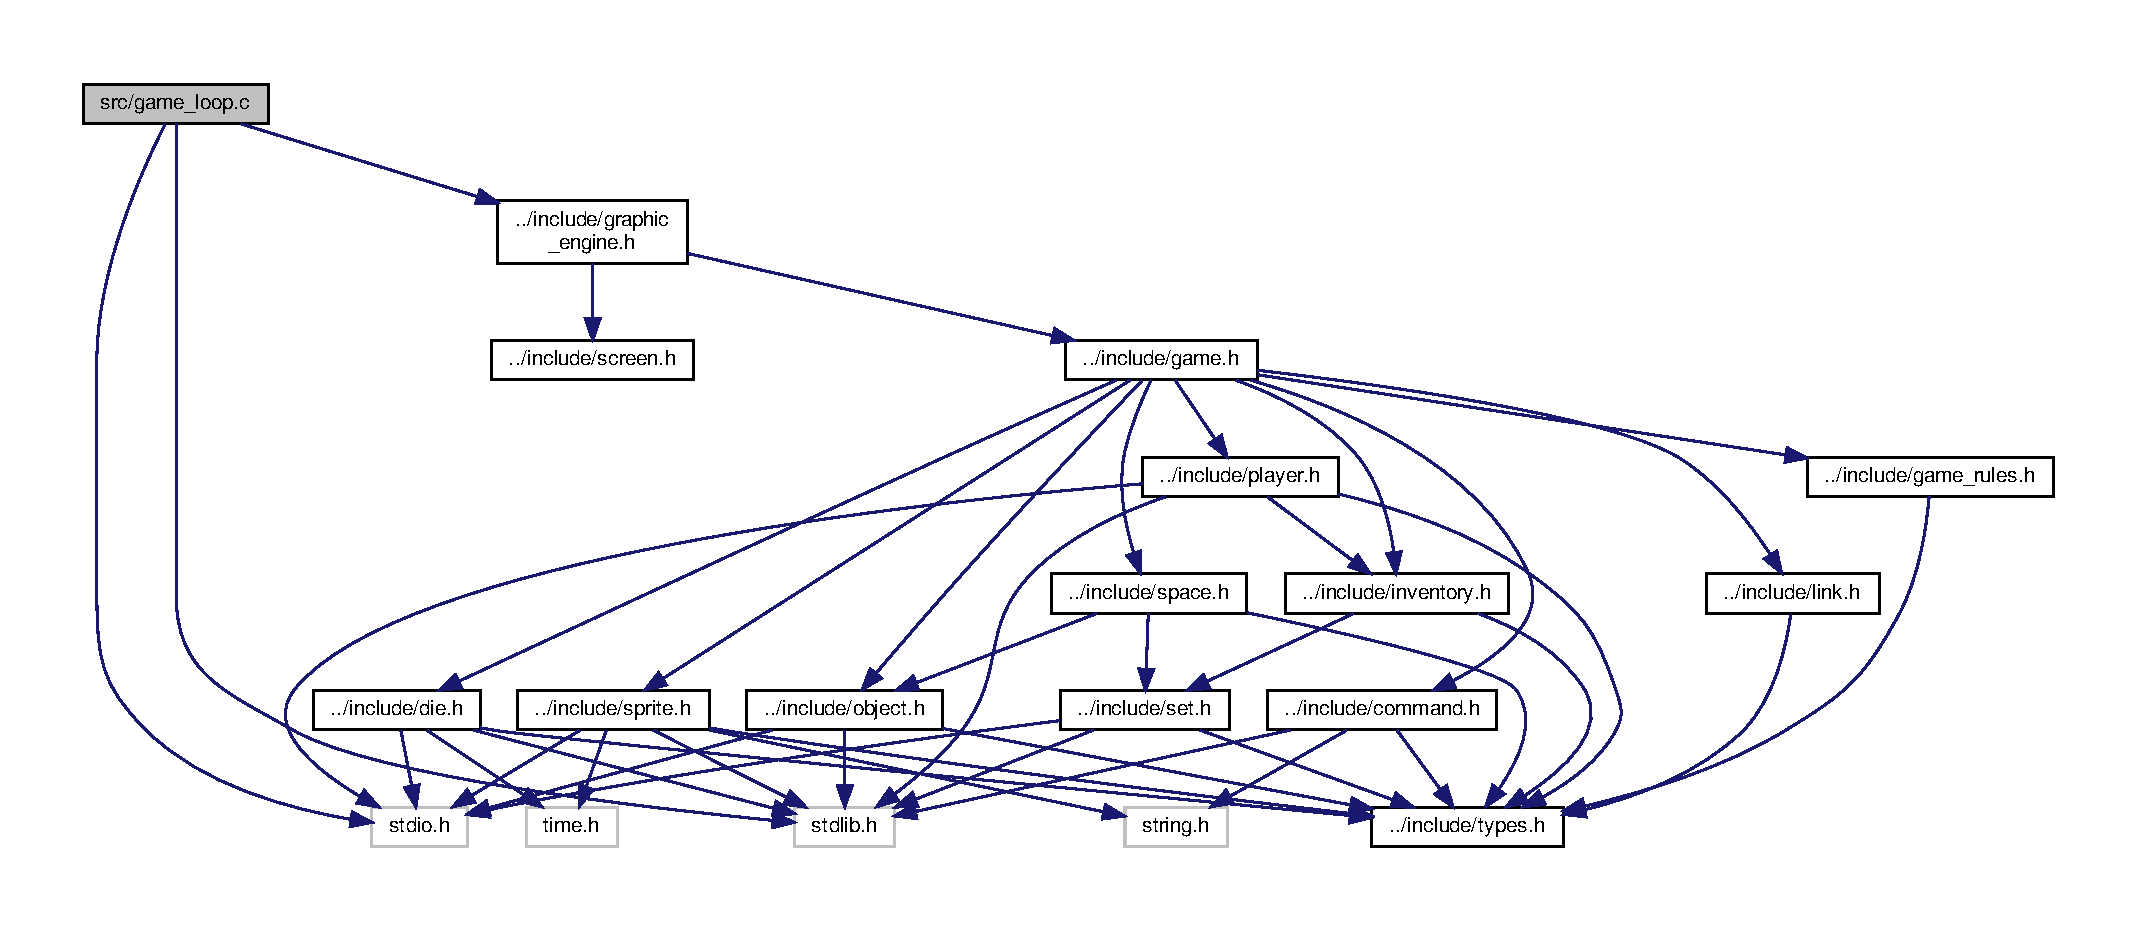
\includegraphics[width=350pt]{game__loop_8c__incl}
\end{center}
\end{figure}
\subsection*{Functions}
\begin{DoxyCompactItemize}
\item 
int \hyperlink{game__loop_8c_a0ddf1224851353fc92bfbff6f499fa97}{main} (int argc, char $\ast$argv\mbox{[}$\,$\mbox{]})
\end{DoxyCompactItemize}


\subsection{Detailed Description}
Main loop. 

\begin{DoxyAuthor}{Author}
Antonio Solana 
\end{DoxyAuthor}
\begin{DoxyCopyright}{Copyright}
G\+NU Public License 
\end{DoxyCopyright}


\subsection{Function Documentation}
\index{game\+\_\+loop.\+c@{game\+\_\+loop.\+c}!main@{main}}
\index{main@{main}!game\+\_\+loop.\+c@{game\+\_\+loop.\+c}}
\subsubsection[{\texorpdfstring{main(int argc, char $\ast$argv[])}{main(int argc, char *argv[])}}]{\setlength{\rightskip}{0pt plus 5cm}int main (
\begin{DoxyParamCaption}
\item[{int}]{argc, }
\item[{char $\ast$}]{argv\mbox{[}$\,$\mbox{]}}
\end{DoxyParamCaption}
)}\hypertarget{game__loop_8c_a0ddf1224851353fc92bfbff6f499fa97}{}\label{game__loop_8c_a0ddf1224851353fc92bfbff6f499fa97}

\hypertarget{game__reader_8c}{}\section{src/game\+\_\+reader.c File Reference}
\label{game__reader_8c}\index{src/game\+\_\+reader.\+c@{src/game\+\_\+reader.\+c}}


Reads data for the game from files.  


{\ttfamily \#include $<$stdio.\+h$>$}\newline
{\ttfamily \#include $<$stdlib.\+h$>$}\newline
{\ttfamily \#include $<$string.\+h$>$}\newline
{\ttfamily \#include \char`\"{}../include/game\+\_\+reader.\+h\char`\"{}}\newline
Include dependency graph for game\+\_\+reader.\+c\+:\nopagebreak
\begin{figure}[H]
\begin{center}
\leavevmode
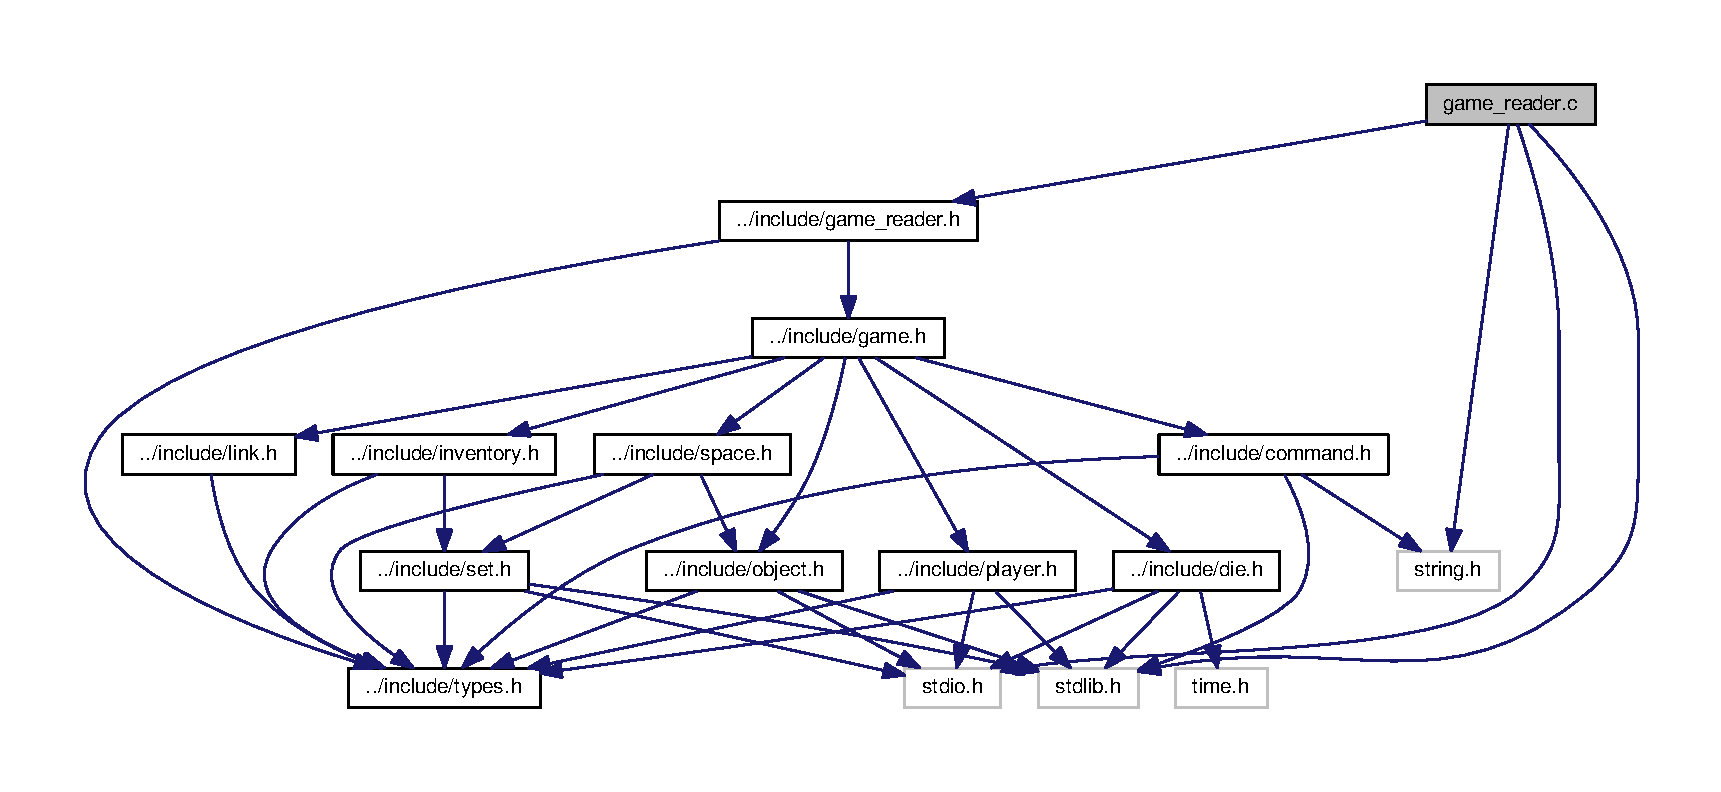
\includegraphics[width=350pt]{game__reader_8c__incl}
\end{center}
\end{figure}
\subsection*{Functions}
\begin{DoxyCompactItemize}
\item 
S\+T\+A\+T\+US \hyperlink{game__reader_8c_a0d01072a28b01545d36240cb8bd9d4f8}{game\+\_\+load\+\_\+spaces} (\hyperlink{struct__Game}{Game} $\ast$game, char $\ast$filename)
\begin{DoxyCompactList}\small\item\em Loads the game from a file. \end{DoxyCompactList}\end{DoxyCompactItemize}


\subsection{Detailed Description}
Reads data for the game from files. 

\begin{DoxyAuthor}{Author}
Catalín Rotaru 
\end{DoxyAuthor}
\begin{DoxyCopyright}{Copyright}
G\+NU Public License 
\end{DoxyCopyright}


\subsection{Function Documentation}
\mbox{\Hypertarget{game__reader_8c_a0d01072a28b01545d36240cb8bd9d4f8}\label{game__reader_8c_a0d01072a28b01545d36240cb8bd9d4f8}} 
\index{game\+\_\+reader.\+c@{game\+\_\+reader.\+c}!game\+\_\+load\+\_\+spaces@{game\+\_\+load\+\_\+spaces}}
\index{game\+\_\+load\+\_\+spaces@{game\+\_\+load\+\_\+spaces}!game\+\_\+reader.\+c@{game\+\_\+reader.\+c}}
\subsubsection{\texorpdfstring{game\+\_\+load\+\_\+spaces()}{game\_load\_spaces()}}
{\footnotesize\ttfamily S\+T\+A\+T\+US game\+\_\+load\+\_\+spaces (\begin{DoxyParamCaption}\item[{\hyperlink{struct__Game}{Game} $\ast$}]{game,  }\item[{char $\ast$}]{filename }\end{DoxyParamCaption})}



Loads the game from a file. 

\begin{DoxyAuthor}{Author}
Catalín Rotaru 
\end{DoxyAuthor}

\begin{DoxyParams}{Parameters}
{\em Game$\ast$} & \\
\hline
{\em char$\ast$} & filename \\
\hline
\end{DoxyParams}
\begin{DoxyReturn}{Returns}
S\+T\+A\+T\+US OK or E\+R\+R\+OR 
\end{DoxyReturn}

\begin{DoxyExceptions}{Exceptions}
{\em No} & game or error when opening \\
\hline
\end{DoxyExceptions}

\hypertarget{game__reader_8h}{}\section{game\+\_\+reader.\+h File Reference}
\label{game__reader_8h}\index{game\+\_\+reader.\+h@{game\+\_\+reader.\+h}}


Reads data for the game from files.  


{\ttfamily \#include \char`\"{}../include/types.\+h\char`\"{}}\\*
{\ttfamily \#include \char`\"{}../include/game.\+h\char`\"{}}\\*
Include dependency graph for game\+\_\+reader.\+h\+:\nopagebreak
\begin{figure}[H]
\begin{center}
\leavevmode
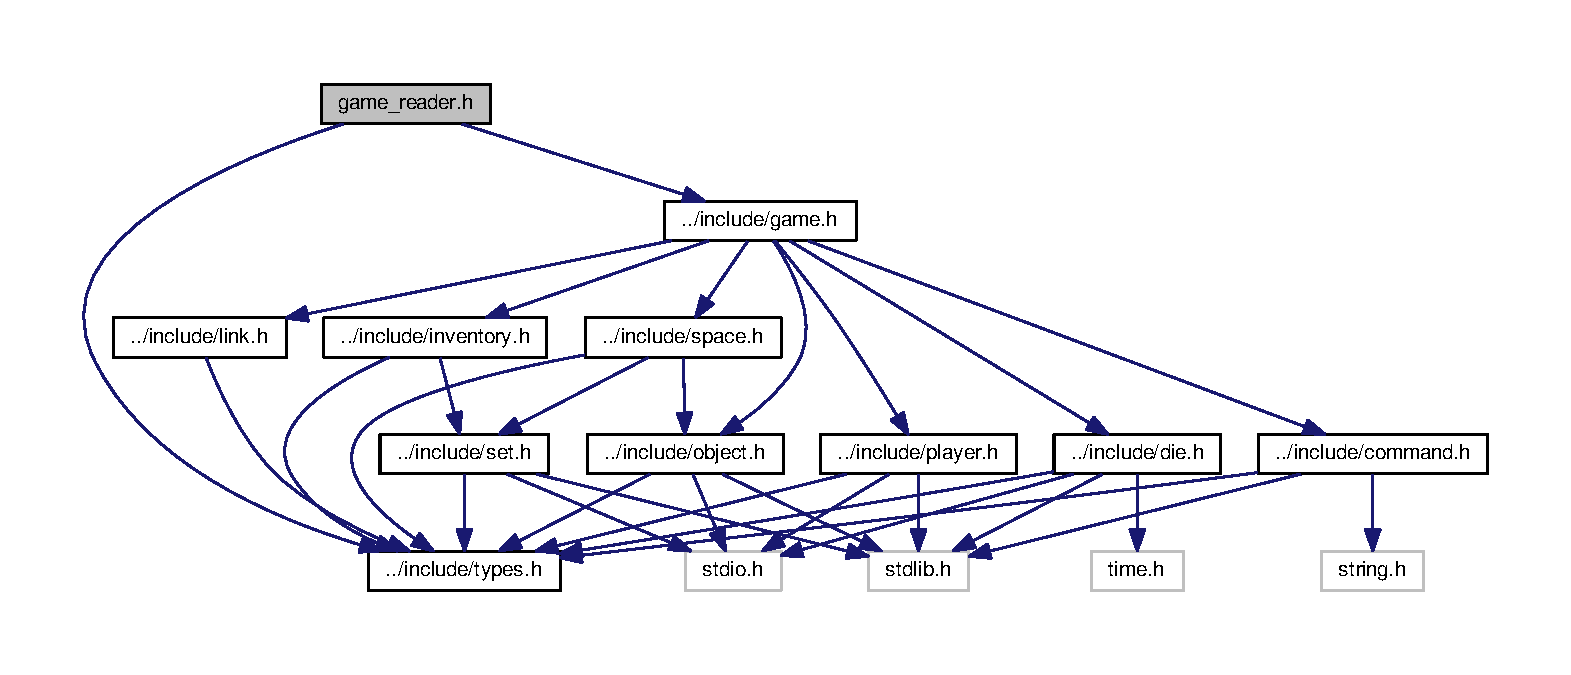
\includegraphics[width=350pt]{game__reader_8h__incl}
\end{center}
\end{figure}
This graph shows which files directly or indirectly include this file\+:\nopagebreak
\begin{figure}[H]
\begin{center}
\leavevmode
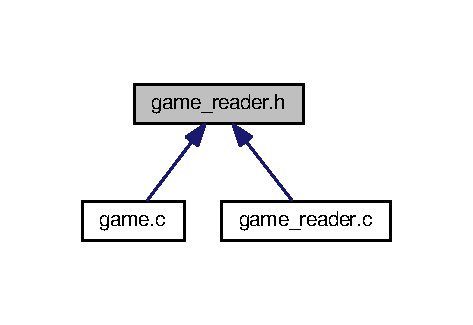
\includegraphics[width=227pt]{game__reader_8h__dep__incl}
\end{center}
\end{figure}
\subsection*{Functions}
\begin{DoxyCompactItemize}
\item 
\hyperlink{types_8h_a32c27cc471df37f4fc818d65de0a56c4}{S\+T\+A\+T\+US} \hyperlink{game__reader_8h_a0d01072a28b01545d36240cb8bd9d4f8}{game\+\_\+load\+\_\+spaces} (\hyperlink{game_8h_a57156d39c530aec3fba3a9dad8c2dc6a}{Game} $\ast$game, char $\ast$filename)
\item 
\hyperlink{types_8h_a32c27cc471df37f4fc818d65de0a56c4}{S\+T\+A\+T\+US} \hyperlink{game__reader_8h_aab4103cf97109ac921f358858ca2684d}{game\+\_\+load\+\_\+links} (\hyperlink{game_8h_a57156d39c530aec3fba3a9dad8c2dc6a}{Game} $\ast$game, char $\ast$filename)
\end{DoxyCompactItemize}


\subsection{Detailed Description}
Reads data for the game from files. 

\begin{DoxyAuthor}{Author}
Catalín Rotaru 
\end{DoxyAuthor}
\begin{DoxyCopyright}{Copyright}
G\+NU Public License 
\end{DoxyCopyright}


\subsection{Function Documentation}
\index{game\+\_\+reader.\+h@{game\+\_\+reader.\+h}!game\+\_\+load\+\_\+links@{game\+\_\+load\+\_\+links}}
\index{game\+\_\+load\+\_\+links@{game\+\_\+load\+\_\+links}!game\+\_\+reader.\+h@{game\+\_\+reader.\+h}}
\subsubsection[{\texorpdfstring{game\+\_\+load\+\_\+links(\+Game $\ast$game, char $\ast$filename)}{game_load_links(Game *game, char *filename)}}]{\setlength{\rightskip}{0pt plus 5cm}{\bf S\+T\+A\+T\+US} game\+\_\+load\+\_\+links (
\begin{DoxyParamCaption}
\item[{{\bf Game} $\ast$}]{game, }
\item[{char $\ast$}]{filename}
\end{DoxyParamCaption}
)}\hypertarget{game__reader_8h_aab4103cf97109ac921f358858ca2684d}{}\label{game__reader_8h_aab4103cf97109ac921f358858ca2684d}
\index{game\+\_\+reader.\+h@{game\+\_\+reader.\+h}!game\+\_\+load\+\_\+spaces@{game\+\_\+load\+\_\+spaces}}
\index{game\+\_\+load\+\_\+spaces@{game\+\_\+load\+\_\+spaces}!game\+\_\+reader.\+h@{game\+\_\+reader.\+h}}
\subsubsection[{\texorpdfstring{game\+\_\+load\+\_\+spaces(\+Game $\ast$game, char $\ast$filename)}{game_load_spaces(Game *game, char *filename)}}]{\setlength{\rightskip}{0pt plus 5cm}{\bf S\+T\+A\+T\+US} game\+\_\+load\+\_\+spaces (
\begin{DoxyParamCaption}
\item[{{\bf Game} $\ast$}]{game, }
\item[{char $\ast$}]{filename}
\end{DoxyParamCaption}
)}\hypertarget{game__reader_8h_a0d01072a28b01545d36240cb8bd9d4f8}{}\label{game__reader_8h_a0d01072a28b01545d36240cb8bd9d4f8}

\hypertarget{game__rules_8c}{}\section{game\+\_\+rules.\+c File Reference}
\label{game__rules_8c}\index{game\+\_\+rules.\+c@{game\+\_\+rules.\+c}}
\subsection*{Functions}
\begin{DoxyCompactItemize}
\item 
\hyperlink{types_8h_a32c27cc471df37f4fc818d65de0a56c4}{S\+T\+A\+T\+US} \hyperlink{game__rules_8c_a73b730a1c123e08e602ddd4f9c8335c2}{update\+\_\+rules} ()
\end{DoxyCompactItemize}


\subsection{Function Documentation}
\index{game\+\_\+rules.\+c@{game\+\_\+rules.\+c}!update\+\_\+rules@{update\+\_\+rules}}
\index{update\+\_\+rules@{update\+\_\+rules}!game\+\_\+rules.\+c@{game\+\_\+rules.\+c}}
\subsubsection[{\texorpdfstring{update\+\_\+rules()}{update_rules()}}]{\setlength{\rightskip}{0pt plus 5cm}{\bf S\+T\+A\+T\+US} update\+\_\+rules (
\begin{DoxyParamCaption}
{}
\end{DoxyParamCaption}
)}\hypertarget{game__rules_8c_a73b730a1c123e08e602ddd4f9c8335c2}{}\label{game__rules_8c_a73b730a1c123e08e602ddd4f9c8335c2}

\hypertarget{game__rules_8h}{}\section{include/game\+\_\+rules.h File Reference}
\label{game__rules_8h}\index{include/game\+\_\+rules.\+h@{include/game\+\_\+rules.\+h}}


Defines input independent actions.  


{\ttfamily \#include \char`\"{}../include/types.\+h\char`\"{}}\newline
Include dependency graph for game\+\_\+rules.\+h\+:\nopagebreak
\begin{figure}[H]
\begin{center}
\leavevmode
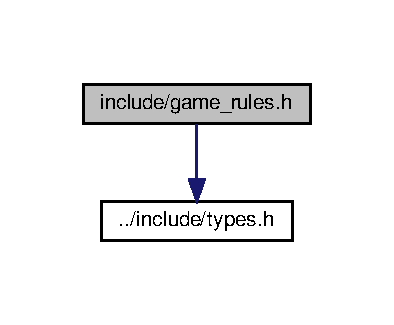
\includegraphics[width=189pt]{game__rules_8h__incl}
\end{center}
\end{figure}
This graph shows which files directly or indirectly include this file\+:\nopagebreak
\begin{figure}[H]
\begin{center}
\leavevmode
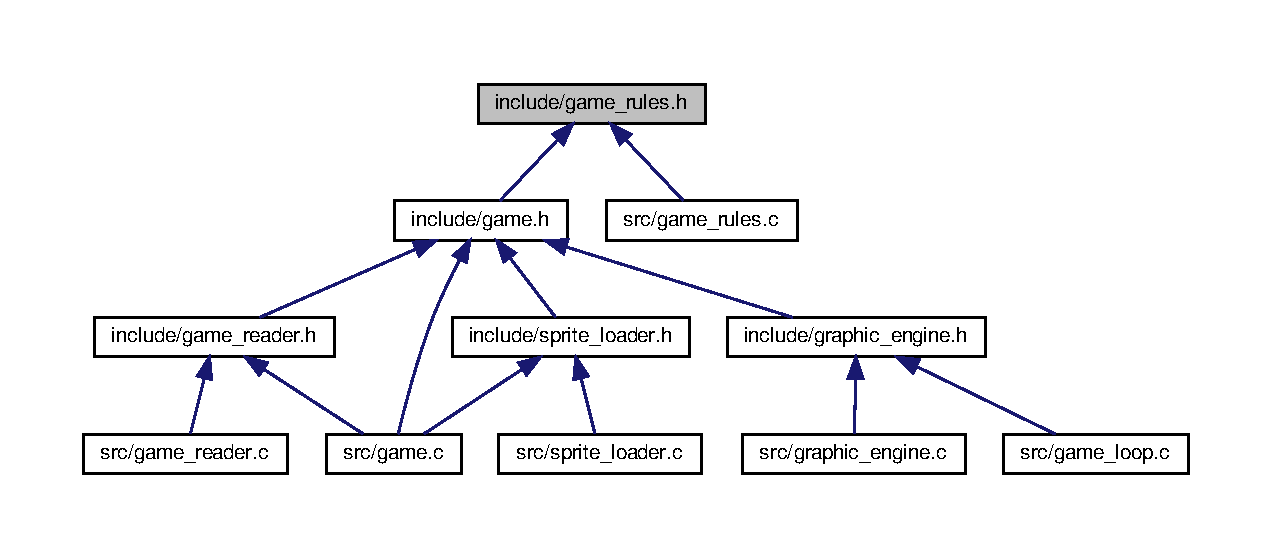
\includegraphics[width=350pt]{game__rules_8h__dep__incl}
\end{center}
\end{figure}
\subsection*{Typedefs}
\begin{DoxyCompactItemize}
\item 
\mbox{\Hypertarget{game__rules_8h_a47319ae4d2cc42513d51c4ede480f91c}\label{game__rules_8h_a47319ae4d2cc42513d51c4ede480f91c}} 
typedef enum enum\+\_\+\+Rules {\bfseries Rules}
\item 
\mbox{\Hypertarget{game__rules_8h_a20d631d93c311ea7d71ceeb04f92811f}\label{game__rules_8h_a20d631d93c311ea7d71ceeb04f92811f}} 
typedef struct \hyperlink{struct__Rule__Data}{\+\_\+\+Rule\+\_\+\+Data} {\bfseries Rule\+\_\+\+Data}
\end{DoxyCompactItemize}
\subsection*{Enumerations}
\begin{DoxyCompactItemize}
\item 
\mbox{\Hypertarget{game__rules_8h_af65db71933f393ce1a8b0c0269987bd4}\label{game__rules_8h_af65db71933f393ce1a8b0c0269987bd4}} 
enum {\bfseries enum\+\_\+\+Rules} \{ \newline
{\bfseries N\+O\+\_\+\+R\+U\+L\+ES}, 
{\bfseries N\+O\+\_\+\+L\+I\+G\+HT}, 
{\bfseries G\+O\+\_\+\+S\+T\+A\+RT}, 
{\bfseries N\+O\+\_\+\+T\+O\+R\+CH}, 
\newline
{\bfseries B\+E\+C\+O\+M\+E\+\_\+\+T\+R\+EE}, 
{\bfseries G\+O\+\_\+\+R\+A\+ND}, 
{\bfseries H\+I\+D\+E\+\_\+\+A\+LL}
 \}
\end{DoxyCompactItemize}
\subsection*{Functions}
\begin{DoxyCompactItemize}
\item 
\hyperlink{struct__Rule__Data}{Rule\+\_\+\+Data} $\ast$ \hyperlink{game__rules_8h_aa59378583b5e1e7926b7a6aacad11069}{rules\+\_\+create} ()
\begin{DoxyCompactList}\small\item\em Creates the rules structure. \end{DoxyCompactList}\item 
void \hyperlink{game__rules_8h_a498223ea63d43e9866d2aef4276ade80}{rules\+\_\+destroy} (\hyperlink{struct__Rule__Data}{Rule\+\_\+\+Data} $\ast$)
\begin{DoxyCompactList}\small\item\em Destroys the rules structure given. \end{DoxyCompactList}\item 
\mbox{\Hypertarget{game__rules_8h_aee8008b425a58b5ef035ebb8d9bc72c7}\label{game__rules_8h_aee8008b425a58b5ef035ebb8d9bc72c7}} 
S\+T\+A\+T\+US {\bfseries rules\+\_\+set\+Move\+Count} (\hyperlink{struct__Rule__Data}{Rule\+\_\+\+Data} $\ast$rule\+\_\+data, int count)
\item 
\mbox{\Hypertarget{game__rules_8h_a99cc10362492baed421118910e43c3ae}\label{game__rules_8h_a99cc10362492baed421118910e43c3ae}} 
S\+T\+A\+T\+US {\bfseries rules\+\_\+set\+Die\+Val} (\hyperlink{struct__Rule__Data}{Rule\+\_\+\+Data} $\ast$rule\+\_\+data, short dieval)
\item 
\mbox{\Hypertarget{game__rules_8h_a7f2de2d6c25cda7f08ab2eb584a37584}\label{game__rules_8h_a7f2de2d6c25cda7f08ab2eb584a37584}} 
int {\bfseries rules\+\_\+get\+Die\+Val} (\hyperlink{struct__Rule__Data}{Rule\+\_\+\+Data} $\ast$rule\+\_\+data)
\item 
\mbox{\Hypertarget{game__rules_8h_aa5818bb2870fb414d05e656f4342fe62}\label{game__rules_8h_aa5818bb2870fb414d05e656f4342fe62}} 
int {\bfseries rules\+\_\+get\+Move\+Count} (\hyperlink{struct__Rule__Data}{Rule\+\_\+\+Data} $\ast$rule\+\_\+data)
\end{DoxyCompactItemize}


\subsection{Detailed Description}
Defines input independent actions. 

\begin{DoxyAuthor}{Author}
Antonio Solana 
\end{DoxyAuthor}
\begin{DoxyCopyright}{Copyright}
G\+NU Public License 
\end{DoxyCopyright}


\subsection{Function Documentation}
\mbox{\Hypertarget{game__rules_8h_aa59378583b5e1e7926b7a6aacad11069}\label{game__rules_8h_aa59378583b5e1e7926b7a6aacad11069}} 
\index{game\+\_\+rules.\+h@{game\+\_\+rules.\+h}!rules\+\_\+create@{rules\+\_\+create}}
\index{rules\+\_\+create@{rules\+\_\+create}!game\+\_\+rules.\+h@{game\+\_\+rules.\+h}}
\subsubsection{\texorpdfstring{rules\+\_\+create()}{rules\_create()}}
{\footnotesize\ttfamily \hyperlink{struct__Rule__Data}{Rule\+\_\+\+Data}$\ast$ rules\+\_\+create (\begin{DoxyParamCaption}{ }\end{DoxyParamCaption})}



Creates the rules structure. 

\begin{DoxyAuthor}{Author}
Antonio Solana 
\end{DoxyAuthor}
\begin{DoxyReturn}{Returns}
Rules\+\_\+\+Data 
\end{DoxyReturn}

\begin{DoxyExceptions}{Exceptions}
{\em Broken} & calloc \\
\hline
\end{DoxyExceptions}
\mbox{\Hypertarget{game__rules_8h_a498223ea63d43e9866d2aef4276ade80}\label{game__rules_8h_a498223ea63d43e9866d2aef4276ade80}} 
\index{game\+\_\+rules.\+h@{game\+\_\+rules.\+h}!rules\+\_\+destroy@{rules\+\_\+destroy}}
\index{rules\+\_\+destroy@{rules\+\_\+destroy}!game\+\_\+rules.\+h@{game\+\_\+rules.\+h}}
\subsubsection{\texorpdfstring{rules\+\_\+destroy()}{rules\_destroy()}}
{\footnotesize\ttfamily void rules\+\_\+destroy (\begin{DoxyParamCaption}\item[{\hyperlink{struct__Rule__Data}{Rule\+\_\+\+Data} $\ast$}]{ }\end{DoxyParamCaption})}



Destroys the rules structure given. 

\begin{DoxyAuthor}{Author}
Antonio Solana 
\end{DoxyAuthor}

\begin{DoxyParams}{Parameters}
{\em Rule\+\_\+\+Data$\ast$} & \\
\hline
\end{DoxyParams}

\hypertarget{graphic__engine_8c}{}\section{graphic\+\_\+engine.\+c File Reference}
\label{graphic__engine_8c}\index{graphic\+\_\+engine.\+c@{graphic\+\_\+engine.\+c}}


Uses screen.$\ast$ to create the UI.  


{\ttfamily \#include $<$stdlib.\+h$>$}\\*
{\ttfamily \#include $<$stdio.\+h$>$}\\*
{\ttfamily \#include \char`\"{}../include/screen.\+h\char`\"{}}\\*
{\ttfamily \#include \char`\"{}../include/graphic\+\_\+engine.\+h\char`\"{}}\\*
{\ttfamily \#include \char`\"{}../include/set.\+h\char`\"{}}\\*
Include dependency graph for graphic\+\_\+engine.\+c\+:
% FIG 0
\subsection*{Classes}
\begin{DoxyCompactItemize}
\item 
struct \hyperlink{struct__Graphic__engine}{\+\_\+\+Graphic\+\_\+engine}
\end{DoxyCompactItemize}
\subsection*{Macros}
\begin{DoxyCompactItemize}
\item 
\#define \hyperlink{graphic__engine_8c_ab4c84d2c2d674e9dde9151e046d28b0c}{S\+T\+D\+\_\+\+S\+P\+A\+CE}~\char`\"{}             \char`\"{}
\item 
\#define \hyperlink{graphic__engine_8c_acc83c571bcd187507ef8320e2ece44fc}{S\+T\+D\+\_\+\+S\+P\+A\+C\+E1}~\char`\"{}    \char`\"{}
\end{DoxyCompactItemize}
\subsection*{Functions}
\begin{DoxyCompactItemize}
\item 
\hyperlink{graphic__engine_8h_ae1bc5cdbfce93098f066274fdea49af1}{Graphic\+\_\+engine} $\ast$ \hyperlink{graphic__engine_8c_a8c3d9abe7282bee1d77d23ea80a4bdec}{graphic\+\_\+engine\+\_\+create} ()
\item 
void \hyperlink{graphic__engine_8c_a5a5eac4ef2033c5ad71aa6895f362f79}{graphic\+\_\+engine\+\_\+destroy} (\hyperlink{graphic__engine_8h_ae1bc5cdbfce93098f066274fdea49af1}{Graphic\+\_\+engine} $\ast$ge)
\item 
void \hyperlink{graphic__engine_8c_a0e275aa477d5fa59e903da33a2a40a5d}{graphic\+\_\+engine\+\_\+paint\+\_\+game} (\hyperlink{graphic__engine_8h_ae1bc5cdbfce93098f066274fdea49af1}{Graphic\+\_\+engine} $\ast$ge, \hyperlink{game_8h_a57156d39c530aec3fba3a9dad8c2dc6a}{Game} $\ast$game)
\item 
void \hyperlink{graphic__engine_8c_ac177bc9048006537b38b7270cb8926ac}{graphic\+\_\+engine\+\_\+paint\+\_\+space} (\hyperlink{graphic__engine_8h_ae1bc5cdbfce93098f066274fdea49af1}{Graphic\+\_\+engine} $\ast$ge, \hyperlink{game_8h_a57156d39c530aec3fba3a9dad8c2dc6a}{Game} $\ast$game, int position\+\_\+of\+\_\+space)
\item 
char $\ast$ \hyperlink{graphic__engine_8c_a6449b0b5144564df757bab40f013eb9c}{create\+\_\+objects\+\_\+string} (\hyperlink{game_8h_a57156d39c530aec3fba3a9dad8c2dc6a}{Game} $\ast$game, \hyperlink{types_8h_a845e604fb28f7e3d97549da3448149d3}{Id} id)
\item 
void \hyperlink{graphic__engine_8c_aaf562c0477dbea81c74a5a74bc8c4e70}{print\+\_\+new\+\_\+line} (\hyperlink{screen_8h_acfdfc42f6522d75fa3c16713afde8127}{Area} $\ast$area, int number)
\end{DoxyCompactItemize}


\subsection{Detailed Description}
Uses screen.$\ast$ to create the UI. 

\begin{DoxyAuthor}{Author}
Antonio Solana 
\end{DoxyAuthor}
\begin{DoxyCopyright}{Copyright}
G\+NU Public License 
\end{DoxyCopyright}


\subsection{Macro Definition Documentation}
\index{graphic\+\_\+engine.\+c@{graphic\+\_\+engine.\+c}!S\+T\+D\+\_\+\+S\+P\+A\+CE@{S\+T\+D\+\_\+\+S\+P\+A\+CE}}
\index{S\+T\+D\+\_\+\+S\+P\+A\+CE@{S\+T\+D\+\_\+\+S\+P\+A\+CE}!graphic\+\_\+engine.\+c@{graphic\+\_\+engine.\+c}}
\subsubsection[{\texorpdfstring{S\+T\+D\+\_\+\+S\+P\+A\+CE}{STD_SPACE}}]{\setlength{\rightskip}{0pt plus 5cm}\#define S\+T\+D\+\_\+\+S\+P\+A\+CE~\char`\"{}             \char`\"{}}\hypertarget{graphic__engine_8c_ab4c84d2c2d674e9dde9151e046d28b0c}{}\label{graphic__engine_8c_ab4c84d2c2d674e9dde9151e046d28b0c}
\index{graphic\+\_\+engine.\+c@{graphic\+\_\+engine.\+c}!S\+T\+D\+\_\+\+S\+P\+A\+C\+E1@{S\+T\+D\+\_\+\+S\+P\+A\+C\+E1}}
\index{S\+T\+D\+\_\+\+S\+P\+A\+C\+E1@{S\+T\+D\+\_\+\+S\+P\+A\+C\+E1}!graphic\+\_\+engine.\+c@{graphic\+\_\+engine.\+c}}
\subsubsection[{\texorpdfstring{S\+T\+D\+\_\+\+S\+P\+A\+C\+E1}{STD_SPACE1}}]{\setlength{\rightskip}{0pt plus 5cm}\#define S\+T\+D\+\_\+\+S\+P\+A\+C\+E1~\char`\"{}    \char`\"{}}\hypertarget{graphic__engine_8c_acc83c571bcd187507ef8320e2ece44fc}{}\label{graphic__engine_8c_acc83c571bcd187507ef8320e2ece44fc}


\subsection{Function Documentation}
\index{graphic\+\_\+engine.\+c@{graphic\+\_\+engine.\+c}!create\+\_\+objects\+\_\+string@{create\+\_\+objects\+\_\+string}}
\index{create\+\_\+objects\+\_\+string@{create\+\_\+objects\+\_\+string}!graphic\+\_\+engine.\+c@{graphic\+\_\+engine.\+c}}
\subsubsection[{\texorpdfstring{create\+\_\+objects\+\_\+string(\+Game $\ast$game, Id id)}{create_objects_string(Game *game, Id id)}}]{\setlength{\rightskip}{0pt plus 5cm}char$\ast$ create\+\_\+objects\+\_\+string (
\begin{DoxyParamCaption}
\item[{{\bf Game} $\ast$}]{game, }
\item[{{\bf Id}}]{id}
\end{DoxyParamCaption}
)}\hypertarget{graphic__engine_8c_a6449b0b5144564df757bab40f013eb9c}{}\label{graphic__engine_8c_a6449b0b5144564df757bab40f013eb9c}
\index{graphic\+\_\+engine.\+c@{graphic\+\_\+engine.\+c}!graphic\+\_\+engine\+\_\+create@{graphic\+\_\+engine\+\_\+create}}
\index{graphic\+\_\+engine\+\_\+create@{graphic\+\_\+engine\+\_\+create}!graphic\+\_\+engine.\+c@{graphic\+\_\+engine.\+c}}
\subsubsection[{\texorpdfstring{graphic\+\_\+engine\+\_\+create()}{graphic_engine_create()}}]{\setlength{\rightskip}{0pt plus 5cm}{\bf Graphic\+\_\+engine}$\ast$ graphic\+\_\+engine\+\_\+create (
\begin{DoxyParamCaption}
{}
\end{DoxyParamCaption}
)}\hypertarget{graphic__engine_8c_a8c3d9abe7282bee1d77d23ea80a4bdec}{}\label{graphic__engine_8c_a8c3d9abe7282bee1d77d23ea80a4bdec}
\index{graphic\+\_\+engine.\+c@{graphic\+\_\+engine.\+c}!graphic\+\_\+engine\+\_\+destroy@{graphic\+\_\+engine\+\_\+destroy}}
\index{graphic\+\_\+engine\+\_\+destroy@{graphic\+\_\+engine\+\_\+destroy}!graphic\+\_\+engine.\+c@{graphic\+\_\+engine.\+c}}
\subsubsection[{\texorpdfstring{graphic\+\_\+engine\+\_\+destroy(\+Graphic\+\_\+engine $\ast$ge)}{graphic_engine_destroy(Graphic_engine *ge)}}]{\setlength{\rightskip}{0pt plus 5cm}void graphic\+\_\+engine\+\_\+destroy (
\begin{DoxyParamCaption}
\item[{{\bf Graphic\+\_\+engine} $\ast$}]{ge}
\end{DoxyParamCaption}
)}\hypertarget{graphic__engine_8c_a5a5eac4ef2033c5ad71aa6895f362f79}{}\label{graphic__engine_8c_a5a5eac4ef2033c5ad71aa6895f362f79}
\index{graphic\+\_\+engine.\+c@{graphic\+\_\+engine.\+c}!graphic\+\_\+engine\+\_\+paint\+\_\+game@{graphic\+\_\+engine\+\_\+paint\+\_\+game}}
\index{graphic\+\_\+engine\+\_\+paint\+\_\+game@{graphic\+\_\+engine\+\_\+paint\+\_\+game}!graphic\+\_\+engine.\+c@{graphic\+\_\+engine.\+c}}
\subsubsection[{\texorpdfstring{graphic\+\_\+engine\+\_\+paint\+\_\+game(\+Graphic\+\_\+engine $\ast$ge, Game $\ast$game)}{graphic_engine_paint_game(Graphic_engine *ge, Game *game)}}]{\setlength{\rightskip}{0pt plus 5cm}void graphic\+\_\+engine\+\_\+paint\+\_\+game (
\begin{DoxyParamCaption}
\item[{{\bf Graphic\+\_\+engine} $\ast$}]{ge, }
\item[{{\bf Game} $\ast$}]{game}
\end{DoxyParamCaption}
)}\hypertarget{graphic__engine_8c_a0e275aa477d5fa59e903da33a2a40a5d}{}\label{graphic__engine_8c_a0e275aa477d5fa59e903da33a2a40a5d}
\index{graphic\+\_\+engine.\+c@{graphic\+\_\+engine.\+c}!graphic\+\_\+engine\+\_\+paint\+\_\+space@{graphic\+\_\+engine\+\_\+paint\+\_\+space}}
\index{graphic\+\_\+engine\+\_\+paint\+\_\+space@{graphic\+\_\+engine\+\_\+paint\+\_\+space}!graphic\+\_\+engine.\+c@{graphic\+\_\+engine.\+c}}
\subsubsection[{\texorpdfstring{graphic\+\_\+engine\+\_\+paint\+\_\+space(\+Graphic\+\_\+engine $\ast$ge, Game $\ast$game, int position\+\_\+of\+\_\+space)}{graphic_engine_paint_space(Graphic_engine *ge, Game *game, int position_of_space)}}]{\setlength{\rightskip}{0pt plus 5cm}void graphic\+\_\+engine\+\_\+paint\+\_\+space (
\begin{DoxyParamCaption}
\item[{{\bf Graphic\+\_\+engine} $\ast$}]{ge, }
\item[{{\bf Game} $\ast$}]{game, }
\item[{int}]{position\+\_\+of\+\_\+space}
\end{DoxyParamCaption}
)}\hypertarget{graphic__engine_8c_ac177bc9048006537b38b7270cb8926ac}{}\label{graphic__engine_8c_ac177bc9048006537b38b7270cb8926ac}
\index{graphic\+\_\+engine.\+c@{graphic\+\_\+engine.\+c}!print\+\_\+new\+\_\+line@{print\+\_\+new\+\_\+line}}
\index{print\+\_\+new\+\_\+line@{print\+\_\+new\+\_\+line}!graphic\+\_\+engine.\+c@{graphic\+\_\+engine.\+c}}
\subsubsection[{\texorpdfstring{print\+\_\+new\+\_\+line(\+Area $\ast$area, int number)}{print_new_line(Area *area, int number)}}]{\setlength{\rightskip}{0pt plus 5cm}void print\+\_\+new\+\_\+line (
\begin{DoxyParamCaption}
\item[{{\bf Area} $\ast$}]{area, }
\item[{int}]{number}
\end{DoxyParamCaption}
)}\hypertarget{graphic__engine_8c_aaf562c0477dbea81c74a5a74bc8c4e70}{}\label{graphic__engine_8c_aaf562c0477dbea81c74a5a74bc8c4e70}

\hypertarget{graphic__engine_8h}{\section{graphic\+\_\+engine.\+h File Reference}
\label{graphic__engine_8h}\index{graphic\+\_\+engine.\+h@{graphic\+\_\+engine.\+h}}
}


Uses screen.$\ast$ to create the U\+I.  


{\ttfamily \#include \char`\"{}../include/game.\+h\char`\"{}}\\*
{\ttfamily \#include \char`\"{}../include/screen.\+h\char`\"{}}\\*
Include dependency graph for graphic\+\_\+engine.\+h\+:\nopagebreak
\begin{figure}[H]
\begin{center}
\leavevmode
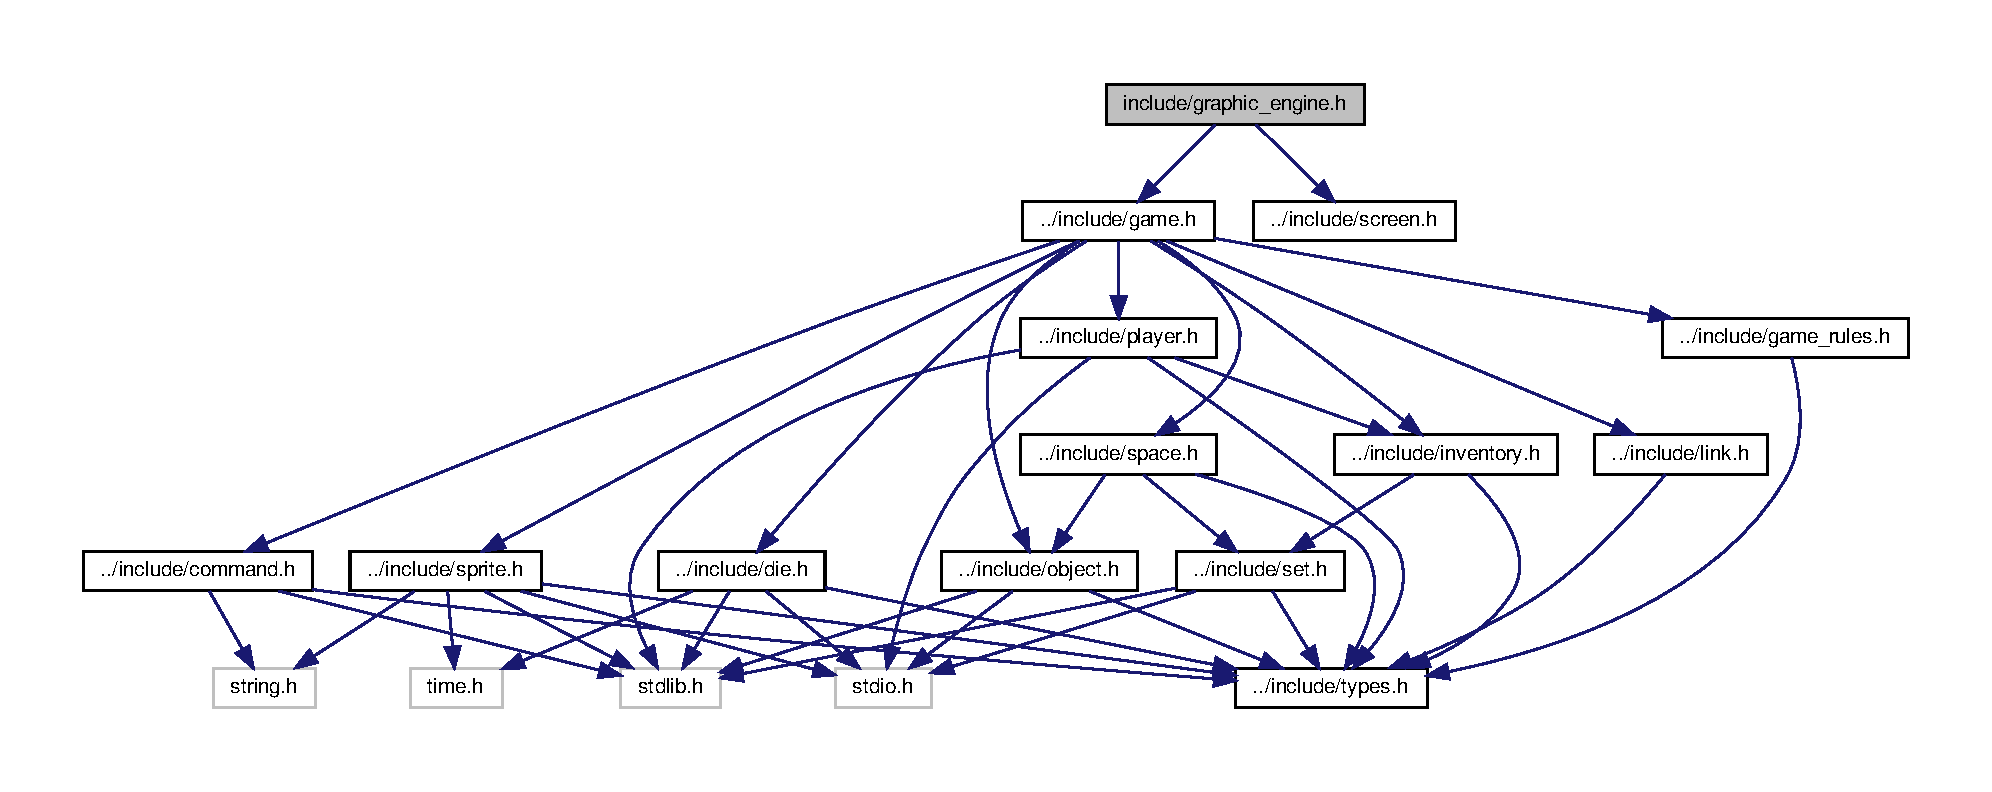
\includegraphics[width=350pt]{graphic__engine_8h__incl}
\end{center}
\end{figure}
This graph shows which files directly or indirectly include this file\+:\nopagebreak
\begin{figure}[H]
\begin{center}
\leavevmode
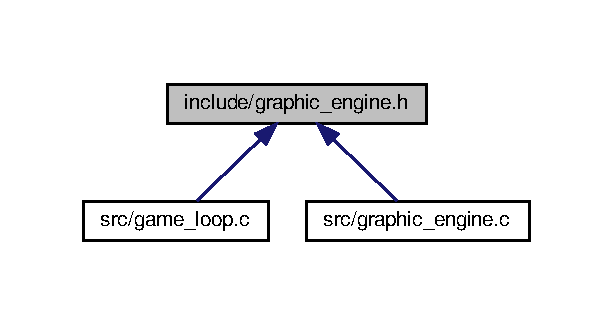
\includegraphics[width=260pt]{graphic__engine_8h__dep__incl}
\end{center}
\end{figure}
\subsection*{Typedefs}
\begin{DoxyCompactItemize}
\item 
typedef struct \hyperlink{struct__Graphic__engine}{\+\_\+\+Graphic\+\_\+engine} \hyperlink{graphic__engine_8h_ae1bc5cdbfce93098f066274fdea49af1}{Graphic\+\_\+engine}
\end{DoxyCompactItemize}
\subsection*{Functions}
\begin{DoxyCompactItemize}
\item 
\hyperlink{graphic__engine_8h_ae1bc5cdbfce93098f066274fdea49af1}{Graphic\+\_\+engine} $\ast$ \hyperlink{graphic__engine_8h_a8c3d9abe7282bee1d77d23ea80a4bdec}{graphic\+\_\+engine\+\_\+create} ()
\item 
void \hyperlink{graphic__engine_8h_a5813ddf7561256cb841f3f62dd41c9c4}{graphic\+\_\+engine\+\_\+destroy} (\hyperlink{graphic__engine_8h_ae1bc5cdbfce93098f066274fdea49af1}{Graphic\+\_\+engine} $\ast$)
\item 
void \hyperlink{graphic__engine_8h_a778819bf85643975da17ff84752495a3}{graphic\+\_\+engine\+\_\+paint\+\_\+game} (\hyperlink{graphic__engine_8h_ae1bc5cdbfce93098f066274fdea49af1}{Graphic\+\_\+engine} $\ast$, \hyperlink{game_8h_a57156d39c530aec3fba3a9dad8c2dc6a}{Game} $\ast$)
\item 
void \hyperlink{graphic__engine_8h_a95c59d3256c61b3c76bf6228e4976924}{graphic\+\_\+engine\+\_\+paint\+\_\+space} (\hyperlink{graphic__engine_8h_ae1bc5cdbfce93098f066274fdea49af1}{Graphic\+\_\+engine} $\ast$, \hyperlink{game_8h_a57156d39c530aec3fba3a9dad8c2dc6a}{Game} $\ast$, int)
\item 
void \hyperlink{graphic__engine_8h_a7c185c973d86fd21f4b6075a215b461a}{print\+\_\+new\+\_\+line} (\hyperlink{screen_8h_acfdfc42f6522d75fa3c16713afde8127}{Area} $\ast$, int number)
\item 
char $\ast$ \hyperlink{graphic__engine_8h_a528b276cbbcb8eb9bb09d20c8ad566b2}{create\+\_\+objects\+\_\+string} (\hyperlink{game_8h_a57156d39c530aec3fba3a9dad8c2dc6a}{Game} $\ast$, \hyperlink{types_8h_a845e604fb28f7e3d97549da3448149d3}{Id})
\end{DoxyCompactItemize}


\subsection{Detailed Description}
Uses screen.$\ast$ to create the U\+I. 

\begin{DoxyAuthor}{Author}
Antonio Solana 
\end{DoxyAuthor}
\begin{DoxyCopyright}{Copyright}
G\+N\+U Public License 
\end{DoxyCopyright}


\subsection{Typedef Documentation}
\hypertarget{graphic__engine_8h_ae1bc5cdbfce93098f066274fdea49af1}{\index{graphic\+\_\+engine.\+h@{graphic\+\_\+engine.\+h}!Graphic\+\_\+engine@{Graphic\+\_\+engine}}
\index{Graphic\+\_\+engine@{Graphic\+\_\+engine}!graphic\+\_\+engine.\+h@{graphic\+\_\+engine.\+h}}
\subsubsection[{Graphic\+\_\+engine}]{\setlength{\rightskip}{0pt plus 5cm}typedef struct {\bf \+\_\+\+Graphic\+\_\+engine} {\bf Graphic\+\_\+engine}}}\label{graphic__engine_8h_ae1bc5cdbfce93098f066274fdea49af1}


\subsection{Function Documentation}
\hypertarget{graphic__engine_8h_a528b276cbbcb8eb9bb09d20c8ad566b2}{\index{graphic\+\_\+engine.\+h@{graphic\+\_\+engine.\+h}!create\+\_\+objects\+\_\+string@{create\+\_\+objects\+\_\+string}}
\index{create\+\_\+objects\+\_\+string@{create\+\_\+objects\+\_\+string}!graphic\+\_\+engine.\+h@{graphic\+\_\+engine.\+h}}
\subsubsection[{create\+\_\+objects\+\_\+string}]{\setlength{\rightskip}{0pt plus 5cm}char$\ast$ create\+\_\+objects\+\_\+string (
\begin{DoxyParamCaption}
\item[{{\bf Game} $\ast$}]{, }
\item[{{\bf Id}}]{}
\end{DoxyParamCaption}
)}}\label{graphic__engine_8h_a528b276cbbcb8eb9bb09d20c8ad566b2}
\hypertarget{graphic__engine_8h_a8c3d9abe7282bee1d77d23ea80a4bdec}{\index{graphic\+\_\+engine.\+h@{graphic\+\_\+engine.\+h}!graphic\+\_\+engine\+\_\+create@{graphic\+\_\+engine\+\_\+create}}
\index{graphic\+\_\+engine\+\_\+create@{graphic\+\_\+engine\+\_\+create}!graphic\+\_\+engine.\+h@{graphic\+\_\+engine.\+h}}
\subsubsection[{graphic\+\_\+engine\+\_\+create}]{\setlength{\rightskip}{0pt plus 5cm}{\bf Graphic\+\_\+engine}$\ast$ graphic\+\_\+engine\+\_\+create (
\begin{DoxyParamCaption}
{}
\end{DoxyParamCaption}
)}}\label{graphic__engine_8h_a8c3d9abe7282bee1d77d23ea80a4bdec}
\hypertarget{graphic__engine_8h_a5813ddf7561256cb841f3f62dd41c9c4}{\index{graphic\+\_\+engine.\+h@{graphic\+\_\+engine.\+h}!graphic\+\_\+engine\+\_\+destroy@{graphic\+\_\+engine\+\_\+destroy}}
\index{graphic\+\_\+engine\+\_\+destroy@{graphic\+\_\+engine\+\_\+destroy}!graphic\+\_\+engine.\+h@{graphic\+\_\+engine.\+h}}
\subsubsection[{graphic\+\_\+engine\+\_\+destroy}]{\setlength{\rightskip}{0pt plus 5cm}void graphic\+\_\+engine\+\_\+destroy (
\begin{DoxyParamCaption}
\item[{{\bf Graphic\+\_\+engine} $\ast$}]{}
\end{DoxyParamCaption}
)}}\label{graphic__engine_8h_a5813ddf7561256cb841f3f62dd41c9c4}
\hypertarget{graphic__engine_8h_a778819bf85643975da17ff84752495a3}{\index{graphic\+\_\+engine.\+h@{graphic\+\_\+engine.\+h}!graphic\+\_\+engine\+\_\+paint\+\_\+game@{graphic\+\_\+engine\+\_\+paint\+\_\+game}}
\index{graphic\+\_\+engine\+\_\+paint\+\_\+game@{graphic\+\_\+engine\+\_\+paint\+\_\+game}!graphic\+\_\+engine.\+h@{graphic\+\_\+engine.\+h}}
\subsubsection[{graphic\+\_\+engine\+\_\+paint\+\_\+game}]{\setlength{\rightskip}{0pt plus 5cm}void graphic\+\_\+engine\+\_\+paint\+\_\+game (
\begin{DoxyParamCaption}
\item[{{\bf Graphic\+\_\+engine} $\ast$}]{, }
\item[{{\bf Game} $\ast$}]{}
\end{DoxyParamCaption}
)}}\label{graphic__engine_8h_a778819bf85643975da17ff84752495a3}
\hypertarget{graphic__engine_8h_a95c59d3256c61b3c76bf6228e4976924}{\index{graphic\+\_\+engine.\+h@{graphic\+\_\+engine.\+h}!graphic\+\_\+engine\+\_\+paint\+\_\+space@{graphic\+\_\+engine\+\_\+paint\+\_\+space}}
\index{graphic\+\_\+engine\+\_\+paint\+\_\+space@{graphic\+\_\+engine\+\_\+paint\+\_\+space}!graphic\+\_\+engine.\+h@{graphic\+\_\+engine.\+h}}
\subsubsection[{graphic\+\_\+engine\+\_\+paint\+\_\+space}]{\setlength{\rightskip}{0pt plus 5cm}void graphic\+\_\+engine\+\_\+paint\+\_\+space (
\begin{DoxyParamCaption}
\item[{{\bf Graphic\+\_\+engine} $\ast$}]{, }
\item[{{\bf Game} $\ast$}]{, }
\item[{int}]{}
\end{DoxyParamCaption}
)}}\label{graphic__engine_8h_a95c59d3256c61b3c76bf6228e4976924}
int = 0 -\/$>$ top space int = 1 -\/$>$ middle space int = 2 -\/$>$ bottom space \hypertarget{graphic__engine_8h_a7c185c973d86fd21f4b6075a215b461a}{\index{graphic\+\_\+engine.\+h@{graphic\+\_\+engine.\+h}!print\+\_\+new\+\_\+line@{print\+\_\+new\+\_\+line}}
\index{print\+\_\+new\+\_\+line@{print\+\_\+new\+\_\+line}!graphic\+\_\+engine.\+h@{graphic\+\_\+engine.\+h}}
\subsubsection[{print\+\_\+new\+\_\+line}]{\setlength{\rightskip}{0pt plus 5cm}void print\+\_\+new\+\_\+line (
\begin{DoxyParamCaption}
\item[{{\bf Area} $\ast$}]{, }
\item[{int}]{number}
\end{DoxyParamCaption}
)}}\label{graphic__engine_8h_a7c185c973d86fd21f4b6075a215b461a}

\hypertarget{inventory_8c}{}\section{src/inventory.c File Reference}
\label{inventory_8c}\index{src/inventory.\+c@{src/inventory.\+c}}


Module for player\textquotesingle{}s inventory.  


{\ttfamily \#include $<$stdio.\+h$>$}\newline
{\ttfamily \#include $<$stdlib.\+h$>$}\newline
{\ttfamily \#include $<$string.\+h$>$}\newline
{\ttfamily \#include \char`\"{}../include/inventory.\+h\char`\"{}}\newline
Include dependency graph for inventory.\+c\+:\nopagebreak
\begin{figure}[H]
\begin{center}
\leavevmode
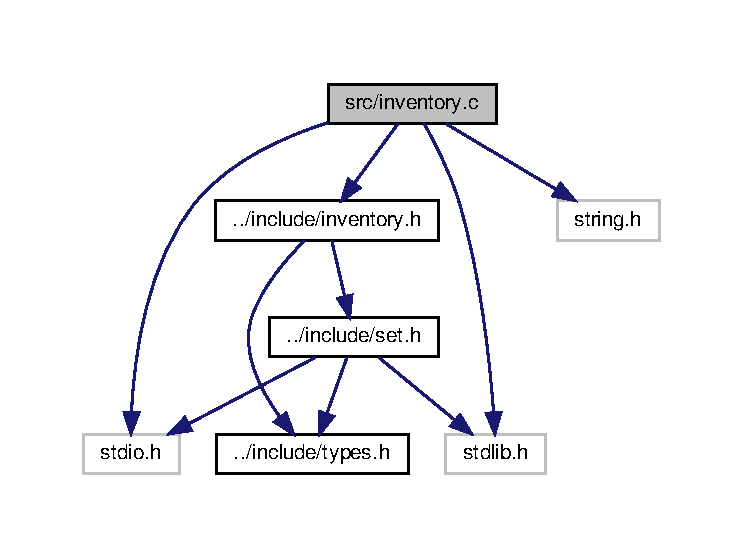
\includegraphics[width=350pt]{inventory_8c__incl}
\end{center}
\end{figure}
\subsection*{Classes}
\begin{DoxyCompactItemize}
\item 
struct \hyperlink{struct__Inventory}{\+\_\+\+Inventory}
\end{DoxyCompactItemize}
\subsection*{Functions}
\begin{DoxyCompactItemize}
\item 
\mbox{\Hypertarget{inventory_8c_a9c1e28ee41fba77e41e9b5241b4db882}\label{inventory_8c_a9c1e28ee41fba77e41e9b5241b4db882}} 
\hyperlink{struct__Inventory}{Inventory} $\ast$ {\bfseries inventory\+\_\+create} (int size)
\item 
\mbox{\Hypertarget{inventory_8c_a670571ee9591b73ca5dfbc0b79b45882}\label{inventory_8c_a670571ee9591b73ca5dfbc0b79b45882}} 
S\+T\+A\+T\+US {\bfseries inventory\+\_\+destroy} (\hyperlink{struct__Inventory}{Inventory} $\ast$inv)
\item 
\mbox{\Hypertarget{inventory_8c_a59ec97ad901a2a8cf48726bf13ee1cbb}\label{inventory_8c_a59ec97ad901a2a8cf48726bf13ee1cbb}} 
S\+T\+A\+T\+US {\bfseries inventory\+\_\+set\+\_\+ids} (\hyperlink{struct__Inventory}{Inventory} $\ast$inv, \hyperlink{struct__Set}{Set} $\ast$ids)
\item 
\mbox{\Hypertarget{inventory_8c_a03ccfae62fdba0dee0ae413a640702ce}\label{inventory_8c_a03ccfae62fdba0dee0ae413a640702ce}} 
\hyperlink{struct__Set}{Set} $\ast$ {\bfseries inventory\+\_\+get\+\_\+ids} (\hyperlink{struct__Inventory}{Inventory} $\ast$inv)
\item 
\mbox{\Hypertarget{inventory_8c_a324cb915fad6eecab9d8494bf149af10}\label{inventory_8c_a324cb915fad6eecab9d8494bf149af10}} 
Id {\bfseries inventory\+\_\+get\+\_\+id\+\_\+at} (\hyperlink{struct__Inventory}{Inventory} $\ast$inv, int num)
\item 
\mbox{\Hypertarget{inventory_8c_a8713e97afcbc73e44bcce7ef446be262}\label{inventory_8c_a8713e97afcbc73e44bcce7ef446be262}} 
S\+T\+A\+T\+US {\bfseries inventory\+\_\+set\+\_\+id\+\_\+max} (\hyperlink{struct__Inventory}{Inventory} $\ast$inv, int id\+\_\+max)
\item 
\mbox{\Hypertarget{inventory_8c_a402a60bdef0a1d2129de827adf64f06a}\label{inventory_8c_a402a60bdef0a1d2129de827adf64f06a}} 
int {\bfseries inventory\+\_\+get\+\_\+id\+\_\+max} (\hyperlink{struct__Inventory}{Inventory} $\ast$inv)
\item 
\mbox{\Hypertarget{inventory_8c_a91549cebec2fd5c6f3ec0c7d6448dc31}\label{inventory_8c_a91549cebec2fd5c6f3ec0c7d6448dc31}} 
S\+T\+A\+T\+US {\bfseries inventory\+\_\+add\+\_\+id} (\hyperlink{struct__Inventory}{Inventory} $\ast$inv, Id id)
\item 
\mbox{\Hypertarget{inventory_8c_abfdd9b2876ee540ae426bfb5b200bf3c}\label{inventory_8c_abfdd9b2876ee540ae426bfb5b200bf3c}} 
S\+T\+A\+T\+US {\bfseries inventory\+\_\+del\+\_\+id} (\hyperlink{struct__Inventory}{Inventory} $\ast$inv, Id id)
\item 
\mbox{\Hypertarget{inventory_8c_a218a121e24cda7abcb77ee745b7d713b}\label{inventory_8c_a218a121e24cda7abcb77ee745b7d713b}} 
B\+O\+OL {\bfseries inventory\+\_\+check\+By\+Id} (\hyperlink{struct__Inventory}{Inventory} $\ast$inv, Id id)
\item 
\mbox{\Hypertarget{inventory_8c_ac4cc8e3348cafe1152499e64cd2737ea}\label{inventory_8c_ac4cc8e3348cafe1152499e64cd2737ea}} 
void {\bfseries inventory\+\_\+print} (\hyperlink{struct__Inventory}{Inventory} $\ast$inv)
\end{DoxyCompactItemize}


\subsection{Detailed Description}
Module for player\textquotesingle{}s inventory. 

\begin{DoxyAuthor}{Author}
Guillermo Ríos 
\end{DoxyAuthor}
\begin{DoxyCopyright}{Copyright}
G\+NU Public License 
\end{DoxyCopyright}

\hypertarget{inventory_8h}{}\section{inventory.\+h File Reference}
\label{inventory_8h}\index{inventory.\+h@{inventory.\+h}}


Module for player\textquotesingle{}s inventory.  


{\ttfamily \#include \char`\"{}../include/types.\+h\char`\"{}}\\*
{\ttfamily \#include \char`\"{}../include/set.\+h\char`\"{}}\\*
Include dependency graph for inventory.\+h\+:
% FIG 0
This graph shows which files directly or indirectly include this file\+:
% FIG 1
\subsection*{Typedefs}
\begin{DoxyCompactItemize}
\item 
typedef struct \hyperlink{struct__Inventory}{\+\_\+\+Inventory} \hyperlink{inventory_8h_a2253bf64ac4ce6a9c1d6f39c0b0d32a3}{Inventory}
\end{DoxyCompactItemize}
\subsection*{Functions}
\begin{DoxyCompactItemize}
\item 
\hyperlink{inventory_8h_a2253bf64ac4ce6a9c1d6f39c0b0d32a3}{Inventory} $\ast$ \hyperlink{inventory_8h_abf1d0e2a115cdef773abf556b3e0947d}{inventory\+\_\+create} (int)
\item 
\hyperlink{types_8h_a32c27cc471df37f4fc818d65de0a56c4}{S\+T\+A\+T\+US} \hyperlink{inventory_8h_a670571ee9591b73ca5dfbc0b79b45882}{inventory\+\_\+destroy} (\hyperlink{inventory_8h_a2253bf64ac4ce6a9c1d6f39c0b0d32a3}{Inventory} $\ast$inv)
\item 
\hyperlink{types_8h_a32c27cc471df37f4fc818d65de0a56c4}{S\+T\+A\+T\+US} \hyperlink{inventory_8h_a59ec97ad901a2a8cf48726bf13ee1cbb}{inventory\+\_\+set\+\_\+ids} (\hyperlink{inventory_8h_a2253bf64ac4ce6a9c1d6f39c0b0d32a3}{Inventory} $\ast$inv, \hyperlink{set_8h_a6d3b7f7c92cbb4577ef3ef7ddbf93161}{Set} $\ast$ids)
\item 
\hyperlink{set_8h_a6d3b7f7c92cbb4577ef3ef7ddbf93161}{Set} $\ast$ \hyperlink{inventory_8h_a03ccfae62fdba0dee0ae413a640702ce}{inventory\+\_\+get\+\_\+ids} (\hyperlink{inventory_8h_a2253bf64ac4ce6a9c1d6f39c0b0d32a3}{Inventory} $\ast$inv)
\item 
\hyperlink{types_8h_a845e604fb28f7e3d97549da3448149d3}{Id} \hyperlink{inventory_8h_a324cb915fad6eecab9d8494bf149af10}{inventory\+\_\+get\+\_\+id\+\_\+at} (\hyperlink{inventory_8h_a2253bf64ac4ce6a9c1d6f39c0b0d32a3}{Inventory} $\ast$inv, int num)
\item 
\hyperlink{types_8h_a32c27cc471df37f4fc818d65de0a56c4}{S\+T\+A\+T\+US} \hyperlink{inventory_8h_a91549cebec2fd5c6f3ec0c7d6448dc31}{inventory\+\_\+add\+\_\+id} (\hyperlink{inventory_8h_a2253bf64ac4ce6a9c1d6f39c0b0d32a3}{Inventory} $\ast$inv, \hyperlink{types_8h_a845e604fb28f7e3d97549da3448149d3}{Id} id)
\item 
\hyperlink{types_8h_a32c27cc471df37f4fc818d65de0a56c4}{S\+T\+A\+T\+US} \hyperlink{inventory_8h_abfdd9b2876ee540ae426bfb5b200bf3c}{inventory\+\_\+del\+\_\+id} (\hyperlink{inventory_8h_a2253bf64ac4ce6a9c1d6f39c0b0d32a3}{Inventory} $\ast$inv, \hyperlink{types_8h_a845e604fb28f7e3d97549da3448149d3}{Id} id)
\item 
void \hyperlink{inventory_8h_a0fc60a571887434cedb4f8b6d1ff69eb}{inventory\+\_\+print} (\hyperlink{inventory_8h_a2253bf64ac4ce6a9c1d6f39c0b0d32a3}{Inventory} $\ast$)
\end{DoxyCompactItemize}


\subsection{Detailed Description}
Module for player\textquotesingle{}s inventory. 

\begin{DoxyAuthor}{Author}
Guillermo Ríos 
\end{DoxyAuthor}
\begin{DoxyCopyright}{Copyright}
G\+NU Public License 
\end{DoxyCopyright}


\subsection{Typedef Documentation}
\index{inventory.\+h@{inventory.\+h}!Inventory@{Inventory}}
\index{Inventory@{Inventory}!inventory.\+h@{inventory.\+h}}
\subsubsection[{\texorpdfstring{Inventory}{Inventory}}]{\setlength{\rightskip}{0pt plus 5cm}typedef struct {\bf \+\_\+\+Inventory} {\bf Inventory}}\hypertarget{inventory_8h_a2253bf64ac4ce6a9c1d6f39c0b0d32a3}{}\label{inventory_8h_a2253bf64ac4ce6a9c1d6f39c0b0d32a3}


\subsection{Function Documentation}
\index{inventory.\+h@{inventory.\+h}!inventory\+\_\+add\+\_\+id@{inventory\+\_\+add\+\_\+id}}
\index{inventory\+\_\+add\+\_\+id@{inventory\+\_\+add\+\_\+id}!inventory.\+h@{inventory.\+h}}
\subsubsection[{\texorpdfstring{inventory\+\_\+add\+\_\+id(\+Inventory $\ast$inv, Id id)}{inventory_add_id(Inventory *inv, Id id)}}]{\setlength{\rightskip}{0pt plus 5cm}{\bf S\+T\+A\+T\+US} inventory\+\_\+add\+\_\+id (
\begin{DoxyParamCaption}
\item[{{\bf Inventory} $\ast$}]{inv, }
\item[{{\bf Id}}]{id}
\end{DoxyParamCaption}
)}\hypertarget{inventory_8h_a91549cebec2fd5c6f3ec0c7d6448dc31}{}\label{inventory_8h_a91549cebec2fd5c6f3ec0c7d6448dc31}
\index{inventory.\+h@{inventory.\+h}!inventory\+\_\+create@{inventory\+\_\+create}}
\index{inventory\+\_\+create@{inventory\+\_\+create}!inventory.\+h@{inventory.\+h}}
\subsubsection[{\texorpdfstring{inventory\+\_\+create(int)}{inventory_create(int)}}]{\setlength{\rightskip}{0pt plus 5cm}{\bf Inventory}$\ast$ inventory\+\_\+create (
\begin{DoxyParamCaption}
\item[{int}]{}
\end{DoxyParamCaption}
)}\hypertarget{inventory_8h_abf1d0e2a115cdef773abf556b3e0947d}{}\label{inventory_8h_abf1d0e2a115cdef773abf556b3e0947d}
\index{inventory.\+h@{inventory.\+h}!inventory\+\_\+del\+\_\+id@{inventory\+\_\+del\+\_\+id}}
\index{inventory\+\_\+del\+\_\+id@{inventory\+\_\+del\+\_\+id}!inventory.\+h@{inventory.\+h}}
\subsubsection[{\texorpdfstring{inventory\+\_\+del\+\_\+id(\+Inventory $\ast$inv, Id id)}{inventory_del_id(Inventory *inv, Id id)}}]{\setlength{\rightskip}{0pt plus 5cm}{\bf S\+T\+A\+T\+US} inventory\+\_\+del\+\_\+id (
\begin{DoxyParamCaption}
\item[{{\bf Inventory} $\ast$}]{inv, }
\item[{{\bf Id}}]{id}
\end{DoxyParamCaption}
)}\hypertarget{inventory_8h_abfdd9b2876ee540ae426bfb5b200bf3c}{}\label{inventory_8h_abfdd9b2876ee540ae426bfb5b200bf3c}
\index{inventory.\+h@{inventory.\+h}!inventory\+\_\+destroy@{inventory\+\_\+destroy}}
\index{inventory\+\_\+destroy@{inventory\+\_\+destroy}!inventory.\+h@{inventory.\+h}}
\subsubsection[{\texorpdfstring{inventory\+\_\+destroy(\+Inventory $\ast$inv)}{inventory_destroy(Inventory *inv)}}]{\setlength{\rightskip}{0pt plus 5cm}{\bf S\+T\+A\+T\+US} inventory\+\_\+destroy (
\begin{DoxyParamCaption}
\item[{{\bf Inventory} $\ast$}]{inv}
\end{DoxyParamCaption}
)}\hypertarget{inventory_8h_a670571ee9591b73ca5dfbc0b79b45882}{}\label{inventory_8h_a670571ee9591b73ca5dfbc0b79b45882}
\index{inventory.\+h@{inventory.\+h}!inventory\+\_\+get\+\_\+id\+\_\+at@{inventory\+\_\+get\+\_\+id\+\_\+at}}
\index{inventory\+\_\+get\+\_\+id\+\_\+at@{inventory\+\_\+get\+\_\+id\+\_\+at}!inventory.\+h@{inventory.\+h}}
\subsubsection[{\texorpdfstring{inventory\+\_\+get\+\_\+id\+\_\+at(\+Inventory $\ast$inv, int num)}{inventory_get_id_at(Inventory *inv, int num)}}]{\setlength{\rightskip}{0pt plus 5cm}{\bf Id} inventory\+\_\+get\+\_\+id\+\_\+at (
\begin{DoxyParamCaption}
\item[{{\bf Inventory} $\ast$}]{inv, }
\item[{int}]{num}
\end{DoxyParamCaption}
)}\hypertarget{inventory_8h_a324cb915fad6eecab9d8494bf149af10}{}\label{inventory_8h_a324cb915fad6eecab9d8494bf149af10}
\index{inventory.\+h@{inventory.\+h}!inventory\+\_\+get\+\_\+ids@{inventory\+\_\+get\+\_\+ids}}
\index{inventory\+\_\+get\+\_\+ids@{inventory\+\_\+get\+\_\+ids}!inventory.\+h@{inventory.\+h}}
\subsubsection[{\texorpdfstring{inventory\+\_\+get\+\_\+ids(\+Inventory $\ast$inv)}{inventory_get_ids(Inventory *inv)}}]{\setlength{\rightskip}{0pt plus 5cm}{\bf Set}$\ast$ inventory\+\_\+get\+\_\+ids (
\begin{DoxyParamCaption}
\item[{{\bf Inventory} $\ast$}]{inv}
\end{DoxyParamCaption}
)}\hypertarget{inventory_8h_a03ccfae62fdba0dee0ae413a640702ce}{}\label{inventory_8h_a03ccfae62fdba0dee0ae413a640702ce}
\index{inventory.\+h@{inventory.\+h}!inventory\+\_\+print@{inventory\+\_\+print}}
\index{inventory\+\_\+print@{inventory\+\_\+print}!inventory.\+h@{inventory.\+h}}
\subsubsection[{\texorpdfstring{inventory\+\_\+print(\+Inventory $\ast$)}{inventory_print(Inventory *)}}]{\setlength{\rightskip}{0pt plus 5cm}void inventory\+\_\+print (
\begin{DoxyParamCaption}
\item[{{\bf Inventory} $\ast$}]{}
\end{DoxyParamCaption}
)}\hypertarget{inventory_8h_a0fc60a571887434cedb4f8b6d1ff69eb}{}\label{inventory_8h_a0fc60a571887434cedb4f8b6d1ff69eb}
\index{inventory.\+h@{inventory.\+h}!inventory\+\_\+set\+\_\+ids@{inventory\+\_\+set\+\_\+ids}}
\index{inventory\+\_\+set\+\_\+ids@{inventory\+\_\+set\+\_\+ids}!inventory.\+h@{inventory.\+h}}
\subsubsection[{\texorpdfstring{inventory\+\_\+set\+\_\+ids(\+Inventory $\ast$inv, Set $\ast$ids)}{inventory_set_ids(Inventory *inv, Set *ids)}}]{\setlength{\rightskip}{0pt plus 5cm}{\bf S\+T\+A\+T\+US} inventory\+\_\+set\+\_\+ids (
\begin{DoxyParamCaption}
\item[{{\bf Inventory} $\ast$}]{inv, }
\item[{{\bf Set} $\ast$}]{ids}
\end{DoxyParamCaption}
)}\hypertarget{inventory_8h_a59ec97ad901a2a8cf48726bf13ee1cbb}{}\label{inventory_8h_a59ec97ad901a2a8cf48726bf13ee1cbb}

\hypertarget{inventory__test_8c}{\section{inventory\+\_\+test.\+c File Reference}
\label{inventory__test_8c}\index{inventory\+\_\+test.\+c@{inventory\+\_\+test.\+c}}
}
{\ttfamily \#include $<$stdio.\+h$>$}\\*
{\ttfamily \#include $<$stdlib.\+h$>$}\\*
{\ttfamily \#include $<$string.\+h$>$}\\*
{\ttfamily \#include \char`\"{}../include/inventory.\+h\char`\"{}}\\*
{\ttfamily \#include \char`\"{}../include/inventory\+\_\+test.\+h\char`\"{}}\\*
{\ttfamily \#include \char`\"{}../include/set.\+h\char`\"{}}\\*
{\ttfamily \#include \char`\"{}../include/test.\+h\char`\"{}}\\*
Include dependency graph for inventory\+\_\+test.\+c\+:\nopagebreak
\begin{figure}[H]
\begin{center}
\leavevmode
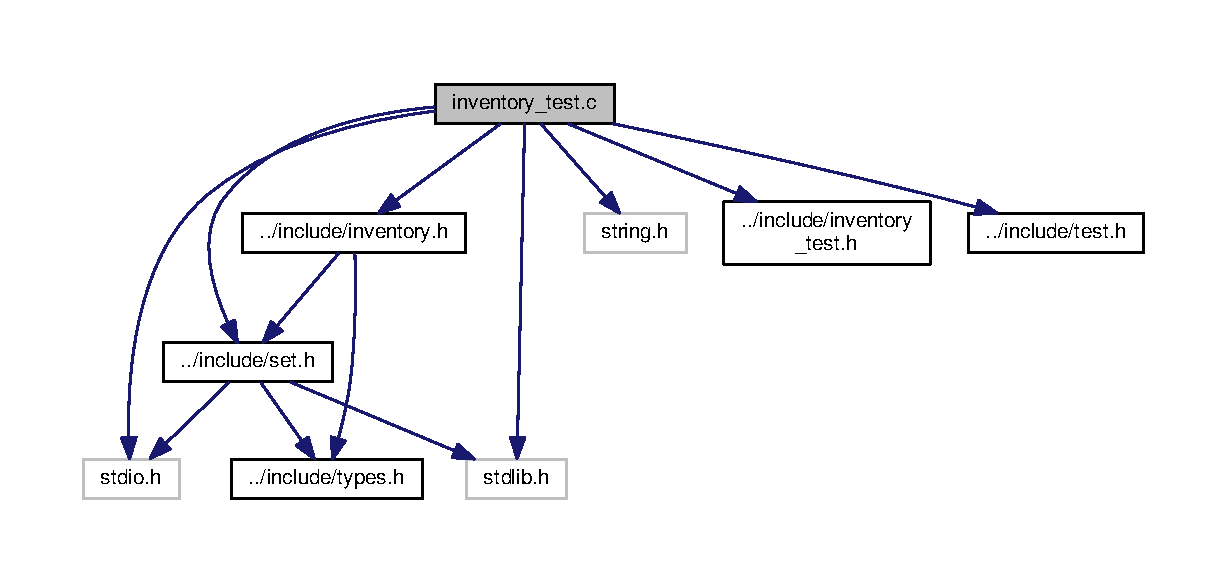
\includegraphics[width=350pt]{inventory__test_8c__incl}
\end{center}
\end{figure}
\subsection*{Macros}
\begin{DoxyCompactItemize}
\item 
\#define \hyperlink{inventory__test_8c_a2a77d2f2c5b698c69c19e1f8782bf709}{M\+A\+X\+\_\+\+T\+E\+S\+T\+S}~9
\end{DoxyCompactItemize}
\subsection*{Functions}
\begin{DoxyCompactItemize}
\item 
int \hyperlink{inventory__test_8c_a3c04138a5bfe5d72780bb7e82a18e627}{main} (int argc, char $\ast$$\ast$argv)
\begin{DoxyCompactList}\small\item\em Funcion principal de pruebas para el modulo Space. \end{DoxyCompactList}\item 
void \hyperlink{inventory__test_8c_a33638f1a88ae16ab8d6bee00145b82b8}{test1\+\_\+inventory\+\_\+create} ()
\item 
void \hyperlink{inventory__test_8c_ae9f44c2019dec9e28f5286bab23d3d3c}{test1\+\_\+inventory\+\_\+set\+\_\+ids} ()
\item 
void \hyperlink{inventory__test_8c_a61bc274b5f03198e98959b9c5dc81453}{test1\+\_\+inventory\+\_\+get\+\_\+ids} ()
\item 
void \hyperlink{inventory__test_8c_adf9ed800874beef00bfc9720398ab440}{test1\+\_\+inventory\+\_\+get\+\_\+id\+\_\+at} ()
\item 
void \hyperlink{inventory__test_8c_ab981fa46131b67fcfa5d22419b8a382b}{test2\+\_\+inventory\+\_\+get\+\_\+id\+\_\+at} ()
\item 
void \hyperlink{inventory__test_8c_a40a21fc4411716ecfa2bbb33c783df94}{test1\+\_\+inventory\+\_\+add\+\_\+id} ()
\item 
void \hyperlink{inventory__test_8c_abfb3407529398f76999549e42d567a7e}{test2\+\_\+inventory\+\_\+add\+\_\+id} ()
\item 
void \hyperlink{inventory__test_8c_a155511682587d9cd63fbd2b62c74dffe}{test1\+\_\+inventory\+\_\+del\+\_\+id} ()
\item 
void \hyperlink{inventory__test_8c_a52850510d17b4f1c105123fdd9e93906}{test2\+\_\+inventory\+\_\+del\+\_\+id} ()
\end{DoxyCompactItemize}


\subsection{Macro Definition Documentation}
\hypertarget{inventory__test_8c_a2a77d2f2c5b698c69c19e1f8782bf709}{\index{inventory\+\_\+test.\+c@{inventory\+\_\+test.\+c}!M\+A\+X\+\_\+\+T\+E\+S\+T\+S@{M\+A\+X\+\_\+\+T\+E\+S\+T\+S}}
\index{M\+A\+X\+\_\+\+T\+E\+S\+T\+S@{M\+A\+X\+\_\+\+T\+E\+S\+T\+S}!inventory\+\_\+test.\+c@{inventory\+\_\+test.\+c}}
\subsubsection[{M\+A\+X\+\_\+\+T\+E\+S\+T\+S}]{\setlength{\rightskip}{0pt plus 5cm}\#define M\+A\+X\+\_\+\+T\+E\+S\+T\+S~9}}\label{inventory__test_8c_a2a77d2f2c5b698c69c19e1f8782bf709}


\subsection{Function Documentation}
\hypertarget{inventory__test_8c_a3c04138a5bfe5d72780bb7e82a18e627}{\index{inventory\+\_\+test.\+c@{inventory\+\_\+test.\+c}!main@{main}}
\index{main@{main}!inventory\+\_\+test.\+c@{inventory\+\_\+test.\+c}}
\subsubsection[{main}]{\setlength{\rightskip}{0pt plus 5cm}int main (
\begin{DoxyParamCaption}
\item[{int}]{argc, }
\item[{char $\ast$$\ast$}]{argv}
\end{DoxyParamCaption}
)}}\label{inventory__test_8c_a3c04138a5bfe5d72780bb7e82a18e627}


Funcion principal de pruebas para el modulo Space. 

Dos modos de ejecucion\+: 1.-\/\+Si se ejecuta sin parametros se ejecutan todas las pruebas 2.-\/\+Si se ejecuta con un numero entre 1 y el numero de pruebas solo ejecuta la prueba indicada \hypertarget{inventory__test_8c_a40a21fc4411716ecfa2bbb33c783df94}{\index{inventory\+\_\+test.\+c@{inventory\+\_\+test.\+c}!test1\+\_\+inventory\+\_\+add\+\_\+id@{test1\+\_\+inventory\+\_\+add\+\_\+id}}
\index{test1\+\_\+inventory\+\_\+add\+\_\+id@{test1\+\_\+inventory\+\_\+add\+\_\+id}!inventory\+\_\+test.\+c@{inventory\+\_\+test.\+c}}
\subsubsection[{test1\+\_\+inventory\+\_\+add\+\_\+id}]{\setlength{\rightskip}{0pt plus 5cm}void test1\+\_\+inventory\+\_\+add\+\_\+id (
\begin{DoxyParamCaption}
{}
\end{DoxyParamCaption}
)}}\label{inventory__test_8c_a40a21fc4411716ecfa2bbb33c783df94}
\hypertarget{inventory__test_8c_a33638f1a88ae16ab8d6bee00145b82b8}{\index{inventory\+\_\+test.\+c@{inventory\+\_\+test.\+c}!test1\+\_\+inventory\+\_\+create@{test1\+\_\+inventory\+\_\+create}}
\index{test1\+\_\+inventory\+\_\+create@{test1\+\_\+inventory\+\_\+create}!inventory\+\_\+test.\+c@{inventory\+\_\+test.\+c}}
\subsubsection[{test1\+\_\+inventory\+\_\+create}]{\setlength{\rightskip}{0pt plus 5cm}void test1\+\_\+inventory\+\_\+create (
\begin{DoxyParamCaption}
{}
\end{DoxyParamCaption}
)}}\label{inventory__test_8c_a33638f1a88ae16ab8d6bee00145b82b8}
\hypertarget{inventory__test_8c_a155511682587d9cd63fbd2b62c74dffe}{\index{inventory\+\_\+test.\+c@{inventory\+\_\+test.\+c}!test1\+\_\+inventory\+\_\+del\+\_\+id@{test1\+\_\+inventory\+\_\+del\+\_\+id}}
\index{test1\+\_\+inventory\+\_\+del\+\_\+id@{test1\+\_\+inventory\+\_\+del\+\_\+id}!inventory\+\_\+test.\+c@{inventory\+\_\+test.\+c}}
\subsubsection[{test1\+\_\+inventory\+\_\+del\+\_\+id}]{\setlength{\rightskip}{0pt plus 5cm}void test1\+\_\+inventory\+\_\+del\+\_\+id (
\begin{DoxyParamCaption}
{}
\end{DoxyParamCaption}
)}}\label{inventory__test_8c_a155511682587d9cd63fbd2b62c74dffe}
\hypertarget{inventory__test_8c_adf9ed800874beef00bfc9720398ab440}{\index{inventory\+\_\+test.\+c@{inventory\+\_\+test.\+c}!test1\+\_\+inventory\+\_\+get\+\_\+id\+\_\+at@{test1\+\_\+inventory\+\_\+get\+\_\+id\+\_\+at}}
\index{test1\+\_\+inventory\+\_\+get\+\_\+id\+\_\+at@{test1\+\_\+inventory\+\_\+get\+\_\+id\+\_\+at}!inventory\+\_\+test.\+c@{inventory\+\_\+test.\+c}}
\subsubsection[{test1\+\_\+inventory\+\_\+get\+\_\+id\+\_\+at}]{\setlength{\rightskip}{0pt plus 5cm}void test1\+\_\+inventory\+\_\+get\+\_\+id\+\_\+at (
\begin{DoxyParamCaption}
{}
\end{DoxyParamCaption}
)}}\label{inventory__test_8c_adf9ed800874beef00bfc9720398ab440}
\hypertarget{inventory__test_8c_a61bc274b5f03198e98959b9c5dc81453}{\index{inventory\+\_\+test.\+c@{inventory\+\_\+test.\+c}!test1\+\_\+inventory\+\_\+get\+\_\+ids@{test1\+\_\+inventory\+\_\+get\+\_\+ids}}
\index{test1\+\_\+inventory\+\_\+get\+\_\+ids@{test1\+\_\+inventory\+\_\+get\+\_\+ids}!inventory\+\_\+test.\+c@{inventory\+\_\+test.\+c}}
\subsubsection[{test1\+\_\+inventory\+\_\+get\+\_\+ids}]{\setlength{\rightskip}{0pt plus 5cm}void test1\+\_\+inventory\+\_\+get\+\_\+ids (
\begin{DoxyParamCaption}
{}
\end{DoxyParamCaption}
)}}\label{inventory__test_8c_a61bc274b5f03198e98959b9c5dc81453}
\hypertarget{inventory__test_8c_ae9f44c2019dec9e28f5286bab23d3d3c}{\index{inventory\+\_\+test.\+c@{inventory\+\_\+test.\+c}!test1\+\_\+inventory\+\_\+set\+\_\+ids@{test1\+\_\+inventory\+\_\+set\+\_\+ids}}
\index{test1\+\_\+inventory\+\_\+set\+\_\+ids@{test1\+\_\+inventory\+\_\+set\+\_\+ids}!inventory\+\_\+test.\+c@{inventory\+\_\+test.\+c}}
\subsubsection[{test1\+\_\+inventory\+\_\+set\+\_\+ids}]{\setlength{\rightskip}{0pt plus 5cm}void test1\+\_\+inventory\+\_\+set\+\_\+ids (
\begin{DoxyParamCaption}
{}
\end{DoxyParamCaption}
)}}\label{inventory__test_8c_ae9f44c2019dec9e28f5286bab23d3d3c}
\hypertarget{inventory__test_8c_abfb3407529398f76999549e42d567a7e}{\index{inventory\+\_\+test.\+c@{inventory\+\_\+test.\+c}!test2\+\_\+inventory\+\_\+add\+\_\+id@{test2\+\_\+inventory\+\_\+add\+\_\+id}}
\index{test2\+\_\+inventory\+\_\+add\+\_\+id@{test2\+\_\+inventory\+\_\+add\+\_\+id}!inventory\+\_\+test.\+c@{inventory\+\_\+test.\+c}}
\subsubsection[{test2\+\_\+inventory\+\_\+add\+\_\+id}]{\setlength{\rightskip}{0pt plus 5cm}void test2\+\_\+inventory\+\_\+add\+\_\+id (
\begin{DoxyParamCaption}
{}
\end{DoxyParamCaption}
)}}\label{inventory__test_8c_abfb3407529398f76999549e42d567a7e}
\hypertarget{inventory__test_8c_a52850510d17b4f1c105123fdd9e93906}{\index{inventory\+\_\+test.\+c@{inventory\+\_\+test.\+c}!test2\+\_\+inventory\+\_\+del\+\_\+id@{test2\+\_\+inventory\+\_\+del\+\_\+id}}
\index{test2\+\_\+inventory\+\_\+del\+\_\+id@{test2\+\_\+inventory\+\_\+del\+\_\+id}!inventory\+\_\+test.\+c@{inventory\+\_\+test.\+c}}
\subsubsection[{test2\+\_\+inventory\+\_\+del\+\_\+id}]{\setlength{\rightskip}{0pt plus 5cm}void test2\+\_\+inventory\+\_\+del\+\_\+id (
\begin{DoxyParamCaption}
{}
\end{DoxyParamCaption}
)}}\label{inventory__test_8c_a52850510d17b4f1c105123fdd9e93906}
\hypertarget{inventory__test_8c_ab981fa46131b67fcfa5d22419b8a382b}{\index{inventory\+\_\+test.\+c@{inventory\+\_\+test.\+c}!test2\+\_\+inventory\+\_\+get\+\_\+id\+\_\+at@{test2\+\_\+inventory\+\_\+get\+\_\+id\+\_\+at}}
\index{test2\+\_\+inventory\+\_\+get\+\_\+id\+\_\+at@{test2\+\_\+inventory\+\_\+get\+\_\+id\+\_\+at}!inventory\+\_\+test.\+c@{inventory\+\_\+test.\+c}}
\subsubsection[{test2\+\_\+inventory\+\_\+get\+\_\+id\+\_\+at}]{\setlength{\rightskip}{0pt plus 5cm}void test2\+\_\+inventory\+\_\+get\+\_\+id\+\_\+at (
\begin{DoxyParamCaption}
{}
\end{DoxyParamCaption}
)}}\label{inventory__test_8c_ab981fa46131b67fcfa5d22419b8a382b}

\hypertarget{inventory__test_8h}{}\section{include/inventory\+\_\+test.h File Reference}
\label{inventory__test_8h}\index{include/inventory\+\_\+test.\+h@{include/inventory\+\_\+test.\+h}}


It declares the tests for the inventory module.  


\subsection*{Functions}
\begin{DoxyCompactItemize}
\item 
\mbox{\Hypertarget{inventory__test_8h_a33638f1a88ae16ab8d6bee00145b82b8}\label{inventory__test_8h_a33638f1a88ae16ab8d6bee00145b82b8}} 
void {\bfseries test1\+\_\+inventory\+\_\+create} ()
\item 
\mbox{\Hypertarget{inventory__test_8h_a7eb3ba387e33c42ff45331c9d9aada34}\label{inventory__test_8h_a7eb3ba387e33c42ff45331c9d9aada34}} 
void {\bfseries test1\+\_\+inventory\+\_\+is\+\_\+full} ()
\item 
\mbox{\Hypertarget{inventory__test_8h_a1c9e567d4919d5aaccc9580815a8a81d}\label{inventory__test_8h_a1c9e567d4919d5aaccc9580815a8a81d}} 
void {\bfseries test2\+\_\+inventory\+\_\+is\+\_\+full} ()
\item 
\mbox{\Hypertarget{inventory__test_8h_afe8c9730e30b58535afc0481970ab2b1}\label{inventory__test_8h_afe8c9730e30b58535afc0481970ab2b1}} 
void {\bfseries test1\+\_\+inventory\+\_\+is\+\_\+empty} ()
\item 
\mbox{\Hypertarget{inventory__test_8h_a4d2a2a4d4ba59446d013debfe9bf05dc}\label{inventory__test_8h_a4d2a2a4d4ba59446d013debfe9bf05dc}} 
void {\bfseries test2\+\_\+inventory\+\_\+is\+\_\+empty} ()
\item 
\mbox{\Hypertarget{inventory__test_8h_ae9f44c2019dec9e28f5286bab23d3d3c}\label{inventory__test_8h_ae9f44c2019dec9e28f5286bab23d3d3c}} 
void {\bfseries test1\+\_\+inventory\+\_\+set\+\_\+ids} ()
\item 
\mbox{\Hypertarget{inventory__test_8h_a61bc274b5f03198e98959b9c5dc81453}\label{inventory__test_8h_a61bc274b5f03198e98959b9c5dc81453}} 
void {\bfseries test1\+\_\+inventory\+\_\+get\+\_\+ids} ()
\item 
\mbox{\Hypertarget{inventory__test_8h_adf9ed800874beef00bfc9720398ab440}\label{inventory__test_8h_adf9ed800874beef00bfc9720398ab440}} 
void {\bfseries test1\+\_\+inventory\+\_\+get\+\_\+id\+\_\+at} ()
\item 
\mbox{\Hypertarget{inventory__test_8h_ab981fa46131b67fcfa5d22419b8a382b}\label{inventory__test_8h_ab981fa46131b67fcfa5d22419b8a382b}} 
void {\bfseries test2\+\_\+inventory\+\_\+get\+\_\+id\+\_\+at} ()
\item 
\mbox{\Hypertarget{inventory__test_8h_a54de162acad19de88c02e72f9db5cc27}\label{inventory__test_8h_a54de162acad19de88c02e72f9db5cc27}} 
void {\bfseries test1\+\_\+inventory\+\_\+set\+\_\+max} ()
\item 
\mbox{\Hypertarget{inventory__test_8h_a283a52426a084b058f3f932a47c16f7d}\label{inventory__test_8h_a283a52426a084b058f3f932a47c16f7d}} 
void {\bfseries test2\+\_\+inventory\+\_\+set\+\_\+max} ()
\item 
\mbox{\Hypertarget{inventory__test_8h_a40a21fc4411716ecfa2bbb33c783df94}\label{inventory__test_8h_a40a21fc4411716ecfa2bbb33c783df94}} 
void {\bfseries test1\+\_\+inventory\+\_\+add\+\_\+id} ()
\item 
\mbox{\Hypertarget{inventory__test_8h_abfb3407529398f76999549e42d567a7e}\label{inventory__test_8h_abfb3407529398f76999549e42d567a7e}} 
void {\bfseries test2\+\_\+inventory\+\_\+add\+\_\+id} ()
\item 
\mbox{\Hypertarget{inventory__test_8h_a155511682587d9cd63fbd2b62c74dffe}\label{inventory__test_8h_a155511682587d9cd63fbd2b62c74dffe}} 
void {\bfseries test1\+\_\+inventory\+\_\+del\+\_\+id} ()
\item 
\mbox{\Hypertarget{inventory__test_8h_a52850510d17b4f1c105123fdd9e93906}\label{inventory__test_8h_a52850510d17b4f1c105123fdd9e93906}} 
void {\bfseries test2\+\_\+inventory\+\_\+del\+\_\+id} ()
\item 
\mbox{\Hypertarget{inventory__test_8h_a17c03f02b989bb00b04155c12fe2af9d}\label{inventory__test_8h_a17c03f02b989bb00b04155c12fe2af9d}} 
void {\bfseries test1\+\_\+inventory\+\_\+get\+\_\+max} ()
\end{DoxyCompactItemize}


\subsection{Detailed Description}
It declares the tests for the inventory module. 

\begin{DoxyAuthor}{Author}
Pablo Sánchez 
\end{DoxyAuthor}
\begin{DoxyCopyright}{Copyright}
G\+NU Public License 
\end{DoxyCopyright}

\hypertarget{link_8c}{\section{link.\+c File Reference}
\label{link_8c}\index{link.\+c@{link.\+c}}
}


Creates the links between spaces.  


{\ttfamily \#include $<$stdio.\+h$>$}\\*
{\ttfamily \#include $<$stdlib.\+h$>$}\\*
{\ttfamily \#include \char`\"{}../include/link.\+h\char`\"{}}\\*
Include dependency graph for link.\+c\+:\nopagebreak
\begin{figure}[H]
\begin{center}
\leavevmode
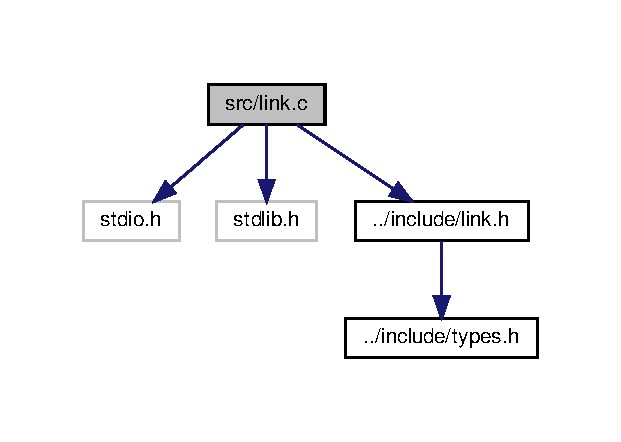
\includegraphics[width=298pt]{link_8c__incl}
\end{center}
\end{figure}
\subsection*{Classes}
\begin{DoxyCompactItemize}
\item 
struct \hyperlink{struct__Link}{\+\_\+\+Link}
\end{DoxyCompactItemize}
\subsection*{Functions}
\begin{DoxyCompactItemize}
\item 
\hyperlink{link_8h_ae3b299941e67be6971bfd64a25505eff}{Link} $\ast$ \hyperlink{link_8c_a8090d7f529cfd6a2fc5df3dd379fe514}{link\+\_\+create} (\hyperlink{types_8h_a845e604fb28f7e3d97549da3448149d3}{Id} id)
\item 
void \hyperlink{link_8c_ad2a9e52ea7c506558a33bb6848bacc4b}{link\+\_\+destroy} (\hyperlink{link_8h_ae3b299941e67be6971bfd64a25505eff}{Link} $\ast$l)
\item 
\hyperlink{types_8h_a32c27cc471df37f4fc818d65de0a56c4}{S\+T\+A\+T\+U\+S} \hyperlink{link_8c_a5c7cbab32fbf5ab20fd041dea9875f39}{link\+\_\+set\+Id} (\hyperlink{link_8h_ae3b299941e67be6971bfd64a25505eff}{Link} $\ast$l, \hyperlink{types_8h_a845e604fb28f7e3d97549da3448149d3}{Id} id)
\item 
\hyperlink{types_8h_a32c27cc471df37f4fc818d65de0a56c4}{S\+T\+A\+T\+U\+S} \hyperlink{link_8c_a085cf528b6faac46522c5f7557f22154}{link\+\_\+set\+Status} (\hyperlink{link_8h_ae3b299941e67be6971bfd64a25505eff}{Link} $\ast$l, \hyperlink{types_8h_aa60f669816b146d6373c62d9625e52ad}{Link\+Status} door)
\item 
\hyperlink{types_8h_a32c27cc471df37f4fc818d65de0a56c4}{S\+T\+A\+T\+U\+S} \hyperlink{link_8c_a894a7b512d0ef47fed125c52fc4efa18}{link\+\_\+set\+Spaces} (\hyperlink{link_8h_ae3b299941e67be6971bfd64a25505eff}{Link} $\ast$l, \hyperlink{types_8h_a845e604fb28f7e3d97549da3448149d3}{Id} space1, \hyperlink{types_8h_a845e604fb28f7e3d97549da3448149d3}{Id} space2)
\item 
\hyperlink{types_8h_a845e604fb28f7e3d97549da3448149d3}{Id} \hyperlink{link_8c_a53c1abc5b1036293b2f083a43fa5f9a6}{link\+\_\+get\+Id} (\hyperlink{link_8h_ae3b299941e67be6971bfd64a25505eff}{Link} $\ast$l)
\item 
\hyperlink{types_8h_a845e604fb28f7e3d97549da3448149d3}{Id} \hyperlink{link_8c_a0a71c306ec967042b34cb06f9c54b120}{link\+\_\+get\+Space1} (\hyperlink{link_8h_ae3b299941e67be6971bfd64a25505eff}{Link} $\ast$l)
\item 
\hyperlink{types_8h_a845e604fb28f7e3d97549da3448149d3}{Id} \hyperlink{link_8c_a7ba54ca1d23bed23f67e059223df27cd}{link\+\_\+get\+Space2} (\hyperlink{link_8h_ae3b299941e67be6971bfd64a25505eff}{Link} $\ast$l)
\item 
\hyperlink{types_8h_aa60f669816b146d6373c62d9625e52ad}{Link\+Status} \hyperlink{link_8c_a41ceb902222cd286d751dad50cac70ba}{link\+\_\+get\+Status} (\hyperlink{link_8h_ae3b299941e67be6971bfd64a25505eff}{Link} $\ast$l)
\item 
\hyperlink{types_8h_a32c27cc471df37f4fc818d65de0a56c4}{S\+T\+A\+T\+U\+S} \hyperlink{link_8c_a95ea756dad592e65440a33dfbe47edcf}{link\+\_\+print} (\hyperlink{link_8h_ae3b299941e67be6971bfd64a25505eff}{Link} $\ast$link)
\item 
\hyperlink{types_8h_a845e604fb28f7e3d97549da3448149d3}{Id} \hyperlink{link_8c_a93f626504aabd27049d5a9e5c2ad9091}{link\+\_\+get\+Destination} (\hyperlink{link_8h_ae3b299941e67be6971bfd64a25505eff}{Link} $\ast$l, \hyperlink{types_8h_a845e604fb28f7e3d97549da3448149d3}{Id} origin\+Id)
\end{DoxyCompactItemize}


\subsection{Detailed Description}
Creates the links between spaces. 

\begin{DoxyAuthor}{Author}
Pablo Sánchez Redondo 
\end{DoxyAuthor}
\begin{DoxyCopyright}{Copyright}
G\+N\+U Public License 
\end{DoxyCopyright}


\subsection{Function Documentation}
\hypertarget{link_8c_a8090d7f529cfd6a2fc5df3dd379fe514}{\index{link.\+c@{link.\+c}!link\+\_\+create@{link\+\_\+create}}
\index{link\+\_\+create@{link\+\_\+create}!link.\+c@{link.\+c}}
\subsubsection[{link\+\_\+create}]{\setlength{\rightskip}{0pt plus 5cm}{\bf Link}$\ast$ link\+\_\+create (
\begin{DoxyParamCaption}
\item[{{\bf Id}}]{id}
\end{DoxyParamCaption}
)}}\label{link_8c_a8090d7f529cfd6a2fc5df3dd379fe514}
\hypertarget{link_8c_ad2a9e52ea7c506558a33bb6848bacc4b}{\index{link.\+c@{link.\+c}!link\+\_\+destroy@{link\+\_\+destroy}}
\index{link\+\_\+destroy@{link\+\_\+destroy}!link.\+c@{link.\+c}}
\subsubsection[{link\+\_\+destroy}]{\setlength{\rightskip}{0pt plus 5cm}void link\+\_\+destroy (
\begin{DoxyParamCaption}
\item[{{\bf Link} $\ast$}]{l}
\end{DoxyParamCaption}
)}}\label{link_8c_ad2a9e52ea7c506558a33bb6848bacc4b}
\hypertarget{link_8c_a93f626504aabd27049d5a9e5c2ad9091}{\index{link.\+c@{link.\+c}!link\+\_\+get\+Destination@{link\+\_\+get\+Destination}}
\index{link\+\_\+get\+Destination@{link\+\_\+get\+Destination}!link.\+c@{link.\+c}}
\subsubsection[{link\+\_\+get\+Destination}]{\setlength{\rightskip}{0pt plus 5cm}{\bf Id} link\+\_\+get\+Destination (
\begin{DoxyParamCaption}
\item[{{\bf Link} $\ast$}]{l, }
\item[{{\bf Id}}]{origin\+Id}
\end{DoxyParamCaption}
)}}\label{link_8c_a93f626504aabd27049d5a9e5c2ad9091}
\hypertarget{link_8c_a53c1abc5b1036293b2f083a43fa5f9a6}{\index{link.\+c@{link.\+c}!link\+\_\+get\+Id@{link\+\_\+get\+Id}}
\index{link\+\_\+get\+Id@{link\+\_\+get\+Id}!link.\+c@{link.\+c}}
\subsubsection[{link\+\_\+get\+Id}]{\setlength{\rightskip}{0pt plus 5cm}{\bf Id} link\+\_\+get\+Id (
\begin{DoxyParamCaption}
\item[{{\bf Link} $\ast$}]{l}
\end{DoxyParamCaption}
)}}\label{link_8c_a53c1abc5b1036293b2f083a43fa5f9a6}
\hypertarget{link_8c_a0a71c306ec967042b34cb06f9c54b120}{\index{link.\+c@{link.\+c}!link\+\_\+get\+Space1@{link\+\_\+get\+Space1}}
\index{link\+\_\+get\+Space1@{link\+\_\+get\+Space1}!link.\+c@{link.\+c}}
\subsubsection[{link\+\_\+get\+Space1}]{\setlength{\rightskip}{0pt plus 5cm}{\bf Id} link\+\_\+get\+Space1 (
\begin{DoxyParamCaption}
\item[{{\bf Link} $\ast$}]{l}
\end{DoxyParamCaption}
)}}\label{link_8c_a0a71c306ec967042b34cb06f9c54b120}
\hypertarget{link_8c_a7ba54ca1d23bed23f67e059223df27cd}{\index{link.\+c@{link.\+c}!link\+\_\+get\+Space2@{link\+\_\+get\+Space2}}
\index{link\+\_\+get\+Space2@{link\+\_\+get\+Space2}!link.\+c@{link.\+c}}
\subsubsection[{link\+\_\+get\+Space2}]{\setlength{\rightskip}{0pt plus 5cm}{\bf Id} link\+\_\+get\+Space2 (
\begin{DoxyParamCaption}
\item[{{\bf Link} $\ast$}]{l}
\end{DoxyParamCaption}
)}}\label{link_8c_a7ba54ca1d23bed23f67e059223df27cd}
\hypertarget{link_8c_a41ceb902222cd286d751dad50cac70ba}{\index{link.\+c@{link.\+c}!link\+\_\+get\+Status@{link\+\_\+get\+Status}}
\index{link\+\_\+get\+Status@{link\+\_\+get\+Status}!link.\+c@{link.\+c}}
\subsubsection[{link\+\_\+get\+Status}]{\setlength{\rightskip}{0pt plus 5cm}{\bf Link\+Status} link\+\_\+get\+Status (
\begin{DoxyParamCaption}
\item[{{\bf Link} $\ast$}]{l}
\end{DoxyParamCaption}
)}}\label{link_8c_a41ceb902222cd286d751dad50cac70ba}
\hypertarget{link_8c_a95ea756dad592e65440a33dfbe47edcf}{\index{link.\+c@{link.\+c}!link\+\_\+print@{link\+\_\+print}}
\index{link\+\_\+print@{link\+\_\+print}!link.\+c@{link.\+c}}
\subsubsection[{link\+\_\+print}]{\setlength{\rightskip}{0pt plus 5cm}{\bf S\+T\+A\+T\+U\+S} link\+\_\+print (
\begin{DoxyParamCaption}
\item[{{\bf Link} $\ast$}]{link}
\end{DoxyParamCaption}
)}}\label{link_8c_a95ea756dad592e65440a33dfbe47edcf}
\hypertarget{link_8c_a5c7cbab32fbf5ab20fd041dea9875f39}{\index{link.\+c@{link.\+c}!link\+\_\+set\+Id@{link\+\_\+set\+Id}}
\index{link\+\_\+set\+Id@{link\+\_\+set\+Id}!link.\+c@{link.\+c}}
\subsubsection[{link\+\_\+set\+Id}]{\setlength{\rightskip}{0pt plus 5cm}{\bf S\+T\+A\+T\+U\+S} link\+\_\+set\+Id (
\begin{DoxyParamCaption}
\item[{{\bf Link} $\ast$}]{l, }
\item[{{\bf Id}}]{id}
\end{DoxyParamCaption}
)}}\label{link_8c_a5c7cbab32fbf5ab20fd041dea9875f39}
\hypertarget{link_8c_a894a7b512d0ef47fed125c52fc4efa18}{\index{link.\+c@{link.\+c}!link\+\_\+set\+Spaces@{link\+\_\+set\+Spaces}}
\index{link\+\_\+set\+Spaces@{link\+\_\+set\+Spaces}!link.\+c@{link.\+c}}
\subsubsection[{link\+\_\+set\+Spaces}]{\setlength{\rightskip}{0pt plus 5cm}{\bf S\+T\+A\+T\+U\+S} link\+\_\+set\+Spaces (
\begin{DoxyParamCaption}
\item[{{\bf Link} $\ast$}]{l, }
\item[{{\bf Id}}]{space1, }
\item[{{\bf Id}}]{space2}
\end{DoxyParamCaption}
)}}\label{link_8c_a894a7b512d0ef47fed125c52fc4efa18}
\hypertarget{link_8c_a085cf528b6faac46522c5f7557f22154}{\index{link.\+c@{link.\+c}!link\+\_\+set\+Status@{link\+\_\+set\+Status}}
\index{link\+\_\+set\+Status@{link\+\_\+set\+Status}!link.\+c@{link.\+c}}
\subsubsection[{link\+\_\+set\+Status}]{\setlength{\rightskip}{0pt plus 5cm}{\bf S\+T\+A\+T\+U\+S} link\+\_\+set\+Status (
\begin{DoxyParamCaption}
\item[{{\bf Link} $\ast$}]{l, }
\item[{{\bf Link\+Status}}]{door}
\end{DoxyParamCaption}
)}}\label{link_8c_a085cf528b6faac46522c5f7557f22154}

\hypertarget{link_8h}{}\section{include/link.h File Reference}
\label{link_8h}\index{include/link.\+h@{include/link.\+h}}


Creates the links between spaces.  


{\ttfamily \#include \char`\"{}../include/types.\+h\char`\"{}}\newline
Include dependency graph for link.\+h\+:\nopagebreak
\begin{figure}[H]
\begin{center}
\leavevmode
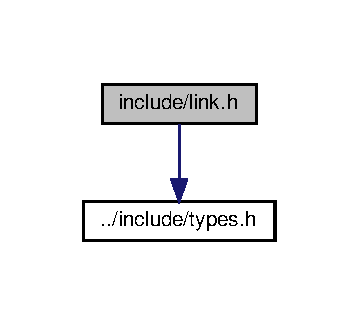
\includegraphics[width=172pt]{link_8h__incl}
\end{center}
\end{figure}
This graph shows which files directly or indirectly include this file\+:\nopagebreak
\begin{figure}[H]
\begin{center}
\leavevmode
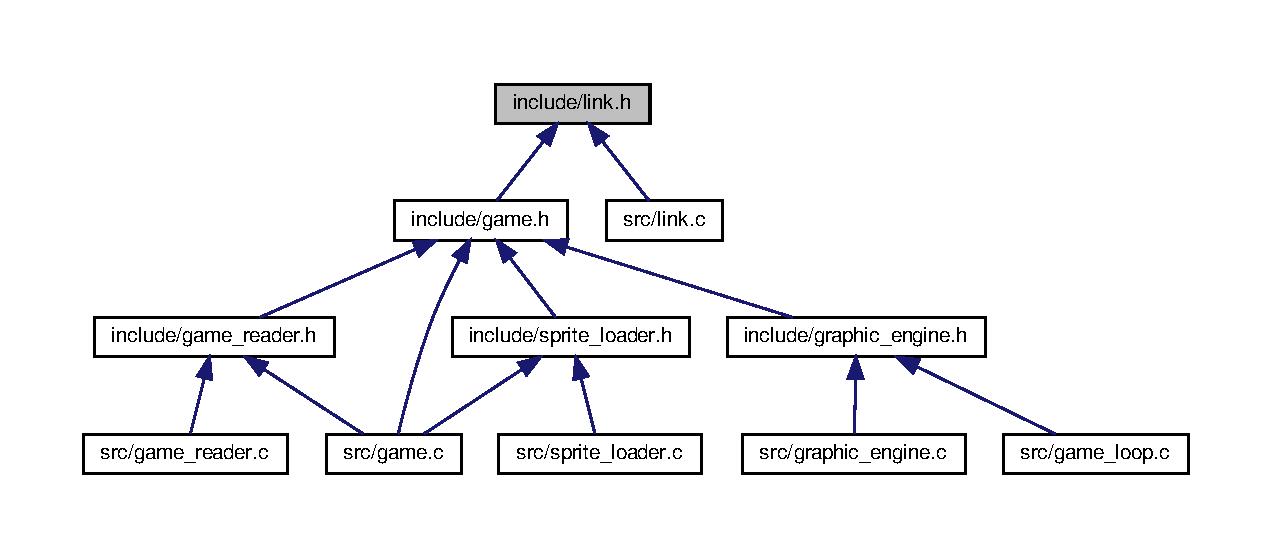
\includegraphics[width=350pt]{link_8h__dep__incl}
\end{center}
\end{figure}
\subsection*{Macros}
\begin{DoxyCompactItemize}
\item 
\mbox{\Hypertarget{link_8h_abfa744c8ca5b46f7f2a10aea53a4ec59}\label{link_8h_abfa744c8ca5b46f7f2a10aea53a4ec59}} 
\#define {\bfseries M\+A\+X\+\_\+\+L\+I\+NK}~1024
\end{DoxyCompactItemize}
\subsection*{Typedefs}
\begin{DoxyCompactItemize}
\item 
\mbox{\Hypertarget{link_8h_ae3b299941e67be6971bfd64a25505eff}\label{link_8h_ae3b299941e67be6971bfd64a25505eff}} 
typedef struct \hyperlink{struct__Link}{\+\_\+\+Link} {\bfseries Link}
\end{DoxyCompactItemize}
\subsection*{Functions}
\begin{DoxyCompactItemize}
\item 
\hyperlink{struct__Link}{Link} $\ast$ \hyperlink{link_8h_ae5986501818a720e4295dc5e634d27f1}{link\+\_\+create} (Id)
\begin{DoxyCompactList}\small\item\em \+: Allocs memory for one link \end{DoxyCompactList}\item 
void \hyperlink{link_8h_a5f40c4fc6fc5696e5f3804bb13c51a0c}{link\+\_\+destroy} (\hyperlink{struct__Link}{Link} $\ast$)
\begin{DoxyCompactList}\small\item\em \+: Frees the Link \end{DoxyCompactList}\item 
S\+T\+A\+T\+US \hyperlink{link_8h_a65bee083bee28569baff6efad72c81a3}{link\+\_\+set\+Id} (\hyperlink{struct__Link}{Link} $\ast$, Id)
\begin{DoxyCompactList}\small\item\em \+: Changes the link id to the given one \end{DoxyCompactList}\item 
S\+T\+A\+T\+US \hyperlink{link_8h_af481cf004c290c67dc9a0139aa6c60b2}{link\+\_\+set\+Status} (\hyperlink{struct__Link}{Link} $\ast$, Link\+Status)
\begin{DoxyCompactList}\small\item\em \+: Changes the Link status to O\+P\+E\+N\+ED or C\+L\+O\+S\+ED \end{DoxyCompactList}\item 
S\+T\+A\+T\+US \hyperlink{link_8h_a3f3b6315bed2368de838d51fdfaa08ef}{link\+\_\+set\+Spaces} (\hyperlink{struct__Link}{Link} $\ast$, Id, Id)
\begin{DoxyCompactList}\small\item\em \+: Sets the spaces the link is joining \end{DoxyCompactList}\item 
Id \hyperlink{link_8h_a43b6a8f4f10bb2fc930e9de2060ebf3e}{link\+\_\+get\+Id} (\hyperlink{struct__Link}{Link} $\ast$)
\begin{DoxyCompactList}\small\item\em \+: Gets the links id \end{DoxyCompactList}\item 
Id \hyperlink{link_8h_ab95e9a5a2fa2204af5b78d51ee6919bb}{link\+\_\+get\+Space1} (\hyperlink{struct__Link}{Link} $\ast$)
\begin{DoxyCompactList}\small\item\em \+: Gets the first Space of the link \end{DoxyCompactList}\item 
Id \hyperlink{link_8h_a29c6680a2a8fdb3afaa7948a4a4f7149}{link\+\_\+get\+Space2} (\hyperlink{struct__Link}{Link} $\ast$)
\begin{DoxyCompactList}\small\item\em \+: Gets the second Space of the link \end{DoxyCompactList}\item 
Link\+Status \hyperlink{link_8h_a72e2c52d52a3d5ba04b816eff098b951}{link\+\_\+get\+Status} (\hyperlink{struct__Link}{Link} $\ast$)
\begin{DoxyCompactList}\small\item\em \+: Gets the status the given link is in \end{DoxyCompactList}\item 
Id \hyperlink{link_8h_a9ce2a73023de210561730e4494ad8734}{link\+\_\+get\+Destination} (\hyperlink{struct__Link}{Link} $\ast$, Id)
\begin{DoxyCompactList}\small\item\em \+: Gets the other space the link is connecting \end{DoxyCompactList}\item 
Id \hyperlink{link_8h_a4eebbdc0a5ac479d126a57e9fef5d9a0}{link\+\_\+get\+Direction} (\hyperlink{struct__Link}{Link} $\ast$)
\begin{DoxyCompactList}\small\item\em \+: Gets the direction of the link (relative to space1) \end{DoxyCompactList}\item 
S\+T\+A\+T\+US \hyperlink{link_8h_a63f1bdc28126b1923590fe67ec93ab4a}{link\+\_\+set\+Direction} (\hyperlink{struct__Link}{Link} $\ast$, int)
\begin{DoxyCompactList}\small\item\em \+: Sets the direction of the link (relative to space1) \end{DoxyCompactList}\item 
S\+T\+A\+T\+US \hyperlink{link_8h_aeabb8b5956d460d0e246d5917478877a}{link\+\_\+print} (\hyperlink{struct__Link}{Link} $\ast$)
\begin{DoxyCompactList}\small\item\em \+: \mbox{[}D\+E\+B\+UG O\+N\+LY\mbox{]} prints the given link in stdout \end{DoxyCompactList}\end{DoxyCompactItemize}


\subsection{Detailed Description}
Creates the links between spaces. 

\begin{DoxyAuthor}{Author}
Pablo Sánchez Redondo 
\end{DoxyAuthor}
\begin{DoxyCopyright}{Copyright}
G\+NU Public License 
\end{DoxyCopyright}


\subsection{Function Documentation}
\mbox{\Hypertarget{link_8h_ae5986501818a720e4295dc5e634d27f1}\label{link_8h_ae5986501818a720e4295dc5e634d27f1}} 
\index{link.\+h@{link.\+h}!link\+\_\+create@{link\+\_\+create}}
\index{link\+\_\+create@{link\+\_\+create}!link.\+h@{link.\+h}}
\subsubsection{\texorpdfstring{link\+\_\+create()}{link\_create()}}
{\footnotesize\ttfamily \hyperlink{struct__Link}{Link}$\ast$ link\+\_\+create (\begin{DoxyParamCaption}\item[{Id}]{ }\end{DoxyParamCaption})}



\+: Allocs memory for one link 

\begin{DoxyAuthor}{Author}
\+: Pablo Sánchez 
\end{DoxyAuthor}

\begin{DoxyParams}{Parameters}
{\em } & \\
\hline
\end{DoxyParams}
\mbox{\Hypertarget{link_8h_a5f40c4fc6fc5696e5f3804bb13c51a0c}\label{link_8h_a5f40c4fc6fc5696e5f3804bb13c51a0c}} 
\index{link.\+h@{link.\+h}!link\+\_\+destroy@{link\+\_\+destroy}}
\index{link\+\_\+destroy@{link\+\_\+destroy}!link.\+h@{link.\+h}}
\subsubsection{\texorpdfstring{link\+\_\+destroy()}{link\_destroy()}}
{\footnotesize\ttfamily void link\+\_\+destroy (\begin{DoxyParamCaption}\item[{\hyperlink{struct__Link}{Link} $\ast$}]{ }\end{DoxyParamCaption})}



\+: Frees the Link 

\begin{DoxyAuthor}{Author}
\+: Pablo Sánchez 
\end{DoxyAuthor}

\begin{DoxyParams}{Parameters}
{\em } & \\
\hline
\end{DoxyParams}
\mbox{\Hypertarget{link_8h_a9ce2a73023de210561730e4494ad8734}\label{link_8h_a9ce2a73023de210561730e4494ad8734}} 
\index{link.\+h@{link.\+h}!link\+\_\+get\+Destination@{link\+\_\+get\+Destination}}
\index{link\+\_\+get\+Destination@{link\+\_\+get\+Destination}!link.\+h@{link.\+h}}
\subsubsection{\texorpdfstring{link\+\_\+get\+Destination()}{link\_getDestination()}}
{\footnotesize\ttfamily Id link\+\_\+get\+Destination (\begin{DoxyParamCaption}\item[{\hyperlink{struct__Link}{Link} $\ast$}]{,  }\item[{Id}]{ }\end{DoxyParamCaption})}



\+: Gets the other space the link is connecting 

\begin{DoxyAuthor}{Author}
\+: Pablo Sánchez 
\end{DoxyAuthor}

\begin{DoxyParams}{Parameters}
{\em } & \\
\hline
\end{DoxyParams}
\mbox{\Hypertarget{link_8h_a4eebbdc0a5ac479d126a57e9fef5d9a0}\label{link_8h_a4eebbdc0a5ac479d126a57e9fef5d9a0}} 
\index{link.\+h@{link.\+h}!link\+\_\+get\+Direction@{link\+\_\+get\+Direction}}
\index{link\+\_\+get\+Direction@{link\+\_\+get\+Direction}!link.\+h@{link.\+h}}
\subsubsection{\texorpdfstring{link\+\_\+get\+Direction()}{link\_getDirection()}}
{\footnotesize\ttfamily Id link\+\_\+get\+Direction (\begin{DoxyParamCaption}\item[{\hyperlink{struct__Link}{Link} $\ast$}]{ }\end{DoxyParamCaption})}



\+: Gets the direction of the link (relative to space1) 

\begin{DoxyAuthor}{Author}
\+: Antonio Solana 
\end{DoxyAuthor}

\begin{DoxyParams}{Parameters}
{\em } & \\
\hline
\end{DoxyParams}
\mbox{\Hypertarget{link_8h_a43b6a8f4f10bb2fc930e9de2060ebf3e}\label{link_8h_a43b6a8f4f10bb2fc930e9de2060ebf3e}} 
\index{link.\+h@{link.\+h}!link\+\_\+get\+Id@{link\+\_\+get\+Id}}
\index{link\+\_\+get\+Id@{link\+\_\+get\+Id}!link.\+h@{link.\+h}}
\subsubsection{\texorpdfstring{link\+\_\+get\+Id()}{link\_getId()}}
{\footnotesize\ttfamily Id link\+\_\+get\+Id (\begin{DoxyParamCaption}\item[{\hyperlink{struct__Link}{Link} $\ast$}]{ }\end{DoxyParamCaption})}



\+: Gets the links id 

\begin{DoxyAuthor}{Author}
\+: Pablo Sánchez 
\end{DoxyAuthor}

\begin{DoxyParams}{Parameters}
{\em } & \\
\hline
\end{DoxyParams}
\mbox{\Hypertarget{link_8h_ab95e9a5a2fa2204af5b78d51ee6919bb}\label{link_8h_ab95e9a5a2fa2204af5b78d51ee6919bb}} 
\index{link.\+h@{link.\+h}!link\+\_\+get\+Space1@{link\+\_\+get\+Space1}}
\index{link\+\_\+get\+Space1@{link\+\_\+get\+Space1}!link.\+h@{link.\+h}}
\subsubsection{\texorpdfstring{link\+\_\+get\+Space1()}{link\_getSpace1()}}
{\footnotesize\ttfamily Id link\+\_\+get\+Space1 (\begin{DoxyParamCaption}\item[{\hyperlink{struct__Link}{Link} $\ast$}]{ }\end{DoxyParamCaption})}



\+: Gets the first Space of the link 

\begin{DoxyAuthor}{Author}
\+: Pablo Sánchez 
\end{DoxyAuthor}

\begin{DoxyParams}{Parameters}
{\em } & \\
\hline
\end{DoxyParams}
\mbox{\Hypertarget{link_8h_a29c6680a2a8fdb3afaa7948a4a4f7149}\label{link_8h_a29c6680a2a8fdb3afaa7948a4a4f7149}} 
\index{link.\+h@{link.\+h}!link\+\_\+get\+Space2@{link\+\_\+get\+Space2}}
\index{link\+\_\+get\+Space2@{link\+\_\+get\+Space2}!link.\+h@{link.\+h}}
\subsubsection{\texorpdfstring{link\+\_\+get\+Space2()}{link\_getSpace2()}}
{\footnotesize\ttfamily Id link\+\_\+get\+Space2 (\begin{DoxyParamCaption}\item[{\hyperlink{struct__Link}{Link} $\ast$}]{ }\end{DoxyParamCaption})}



\+: Gets the second Space of the link 

\begin{DoxyAuthor}{Author}
\+: Pablo Sánchez 
\end{DoxyAuthor}

\begin{DoxyParams}{Parameters}
{\em } & \\
\hline
\end{DoxyParams}
\mbox{\Hypertarget{link_8h_a72e2c52d52a3d5ba04b816eff098b951}\label{link_8h_a72e2c52d52a3d5ba04b816eff098b951}} 
\index{link.\+h@{link.\+h}!link\+\_\+get\+Status@{link\+\_\+get\+Status}}
\index{link\+\_\+get\+Status@{link\+\_\+get\+Status}!link.\+h@{link.\+h}}
\subsubsection{\texorpdfstring{link\+\_\+get\+Status()}{link\_getStatus()}}
{\footnotesize\ttfamily Link\+Status link\+\_\+get\+Status (\begin{DoxyParamCaption}\item[{\hyperlink{struct__Link}{Link} $\ast$}]{ }\end{DoxyParamCaption})}



\+: Gets the status the given link is in 

\begin{DoxyAuthor}{Author}
\+: Pablo Sánchez 
\end{DoxyAuthor}

\begin{DoxyParams}{Parameters}
{\em } & \\
\hline
\end{DoxyParams}
\mbox{\Hypertarget{link_8h_aeabb8b5956d460d0e246d5917478877a}\label{link_8h_aeabb8b5956d460d0e246d5917478877a}} 
\index{link.\+h@{link.\+h}!link\+\_\+print@{link\+\_\+print}}
\index{link\+\_\+print@{link\+\_\+print}!link.\+h@{link.\+h}}
\subsubsection{\texorpdfstring{link\+\_\+print()}{link\_print()}}
{\footnotesize\ttfamily S\+T\+A\+T\+US link\+\_\+print (\begin{DoxyParamCaption}\item[{\hyperlink{struct__Link}{Link} $\ast$}]{ }\end{DoxyParamCaption})}



\+: \mbox{[}D\+E\+B\+UG O\+N\+LY\mbox{]} prints the given link in stdout 

\begin{DoxyAuthor}{Author}
\+: Pablo Sánchez 
\end{DoxyAuthor}

\begin{DoxyParams}{Parameters}
{\em } & \\
\hline
\end{DoxyParams}
\mbox{\Hypertarget{link_8h_a63f1bdc28126b1923590fe67ec93ab4a}\label{link_8h_a63f1bdc28126b1923590fe67ec93ab4a}} 
\index{link.\+h@{link.\+h}!link\+\_\+set\+Direction@{link\+\_\+set\+Direction}}
\index{link\+\_\+set\+Direction@{link\+\_\+set\+Direction}!link.\+h@{link.\+h}}
\subsubsection{\texorpdfstring{link\+\_\+set\+Direction()}{link\_setDirection()}}
{\footnotesize\ttfamily S\+T\+A\+T\+US link\+\_\+set\+Direction (\begin{DoxyParamCaption}\item[{\hyperlink{struct__Link}{Link} $\ast$}]{,  }\item[{int}]{ }\end{DoxyParamCaption})}



\+: Sets the direction of the link (relative to space1) 

\begin{DoxyAuthor}{Author}
\+: Antonio Solana 
\end{DoxyAuthor}

\begin{DoxyParams}{Parameters}
{\em } & \\
\hline
\end{DoxyParams}
\mbox{\Hypertarget{link_8h_a65bee083bee28569baff6efad72c81a3}\label{link_8h_a65bee083bee28569baff6efad72c81a3}} 
\index{link.\+h@{link.\+h}!link\+\_\+set\+Id@{link\+\_\+set\+Id}}
\index{link\+\_\+set\+Id@{link\+\_\+set\+Id}!link.\+h@{link.\+h}}
\subsubsection{\texorpdfstring{link\+\_\+set\+Id()}{link\_setId()}}
{\footnotesize\ttfamily S\+T\+A\+T\+US link\+\_\+set\+Id (\begin{DoxyParamCaption}\item[{\hyperlink{struct__Link}{Link} $\ast$}]{,  }\item[{Id}]{ }\end{DoxyParamCaption})}



\+: Changes the link id to the given one 

\begin{DoxyAuthor}{Author}
\+: Pablo Sánchez 
\end{DoxyAuthor}

\begin{DoxyParams}{Parameters}
{\em } & \\
\hline
\end{DoxyParams}
\mbox{\Hypertarget{link_8h_a3f3b6315bed2368de838d51fdfaa08ef}\label{link_8h_a3f3b6315bed2368de838d51fdfaa08ef}} 
\index{link.\+h@{link.\+h}!link\+\_\+set\+Spaces@{link\+\_\+set\+Spaces}}
\index{link\+\_\+set\+Spaces@{link\+\_\+set\+Spaces}!link.\+h@{link.\+h}}
\subsubsection{\texorpdfstring{link\+\_\+set\+Spaces()}{link\_setSpaces()}}
{\footnotesize\ttfamily S\+T\+A\+T\+US link\+\_\+set\+Spaces (\begin{DoxyParamCaption}\item[{\hyperlink{struct__Link}{Link} $\ast$}]{,  }\item[{Id}]{,  }\item[{Id}]{ }\end{DoxyParamCaption})}



\+: Sets the spaces the link is joining 

\begin{DoxyAuthor}{Author}
\+: Pablo Sánchez 
\end{DoxyAuthor}

\begin{DoxyParams}{Parameters}
{\em } & \\
\hline
\end{DoxyParams}
\mbox{\Hypertarget{link_8h_af481cf004c290c67dc9a0139aa6c60b2}\label{link_8h_af481cf004c290c67dc9a0139aa6c60b2}} 
\index{link.\+h@{link.\+h}!link\+\_\+set\+Status@{link\+\_\+set\+Status}}
\index{link\+\_\+set\+Status@{link\+\_\+set\+Status}!link.\+h@{link.\+h}}
\subsubsection{\texorpdfstring{link\+\_\+set\+Status()}{link\_setStatus()}}
{\footnotesize\ttfamily S\+T\+A\+T\+US link\+\_\+set\+Status (\begin{DoxyParamCaption}\item[{\hyperlink{struct__Link}{Link} $\ast$}]{,  }\item[{Link\+Status}]{ }\end{DoxyParamCaption})}



\+: Changes the Link status to O\+P\+E\+N\+ED or C\+L\+O\+S\+ED 

\begin{DoxyAuthor}{Author}
\+: Pablo Sánchez 
\end{DoxyAuthor}

\begin{DoxyParams}{Parameters}
{\em } & \\
\hline
\end{DoxyParams}

\hypertarget{link__test_8c}{\section{link\+\_\+test.\+c File Reference}
\label{link__test_8c}\index{link\+\_\+test.\+c@{link\+\_\+test.\+c}}
}
{\ttfamily \#include $<$stdio.\+h$>$}\\*
{\ttfamily \#include $<$stdlib.\+h$>$}\\*
{\ttfamily \#include $<$string.\+h$>$}\\*
{\ttfamily \#include \char`\"{}../include/link.\+h\char`\"{}}\\*
{\ttfamily \#include \char`\"{}../include/link\+\_\+test.\+h\char`\"{}}\\*
{\ttfamily \#include \char`\"{}../include/test.\+h\char`\"{}}\\*
Include dependency graph for link\+\_\+test.\+c\+:\nopagebreak
\begin{figure}[H]
\begin{center}
\leavevmode
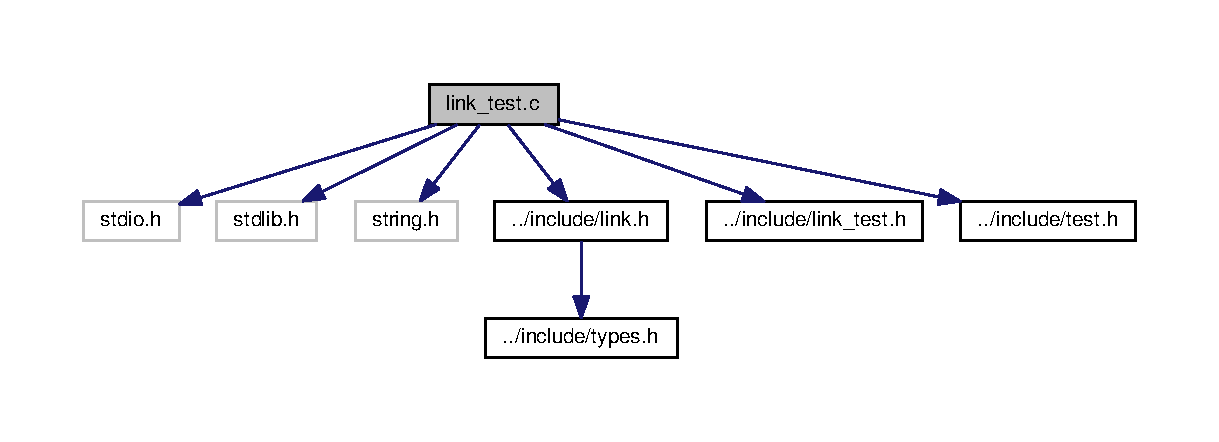
\includegraphics[width=350pt]{link__test_8c__incl}
\end{center}
\end{figure}
\subsection*{Macros}
\begin{DoxyCompactItemize}
\item 
\#define \hyperlink{link__test_8c_a2a77d2f2c5b698c69c19e1f8782bf709}{M\+A\+X\+\_\+\+T\+E\+S\+T\+S}~14
\end{DoxyCompactItemize}
\subsection*{Functions}
\begin{DoxyCompactItemize}
\item 
int \hyperlink{link__test_8c_a3c04138a5bfe5d72780bb7e82a18e627}{main} (int argc, char $\ast$$\ast$argv)
\begin{DoxyCompactList}\small\item\em Funcion principal de pruebas para el modulo Space. \end{DoxyCompactList}\item 
void \hyperlink{link__test_8c_a82c5ee441ad22caad8272212a9e9cc26}{test1\+\_\+link\+\_\+create} ()
\item 
void \hyperlink{link__test_8c_a24b5463da176c3e578b0a0fa8bb1f9f0}{test2\+\_\+link\+\_\+create} ()
\item 
void \hyperlink{link__test_8c_ac2b67785fdf6bb85af93e985af9ee3f2}{test1\+\_\+link\+\_\+set\+\_\+id} ()
\item 
void \hyperlink{link__test_8c_a2f107a28c71f764c8091747f48eaec3f}{test2\+\_\+link\+\_\+set\+\_\+id} ()
\item 
void \hyperlink{link__test_8c_a3b39fdba0c3c967716572bfb01beec27}{test1\+\_\+link\+\_\+set\+\_\+status} ()
\item 
void \hyperlink{link__test_8c_a315ea19cd24434d2153b5df9f372a561}{test2\+\_\+link\+\_\+set\+\_\+status} ()
\item 
void \hyperlink{link__test_8c_ae3df3369cfff931db20aeb87b4a77370}{test1\+\_\+link\+\_\+set\+\_\+spaces} ()
\item 
void \hyperlink{link__test_8c_a98a0815c982a3569c1c8be28f4e13736}{test2\+\_\+link\+\_\+set\+\_\+spaces} ()
\item 
void \hyperlink{link__test_8c_a19c70f79fd51d123173f7aaf6ae50bf8}{test1\+\_\+link\+\_\+get\+\_\+id} ()
\item 
void \hyperlink{link__test_8c_a51cdc27e82c1bac69bdf8702ead4d3d5}{test1\+\_\+link\+\_\+get\+\_\+space1} ()
\item 
void \hyperlink{link__test_8c_ae52422914337fe824858963bf1bb9638}{test1\+\_\+link\+\_\+get\+\_\+space2} ()
\item 
void \hyperlink{link__test_8c_a9f7bf73b9398d551c64f6c845e9e1560}{test1\+\_\+link\+\_\+get\+\_\+status} ()
\item 
void \hyperlink{link__test_8c_ade4160ca2a1f9ae14cff213a241da3fd}{test1\+\_\+link\+\_\+get\+\_\+destination} ()
\end{DoxyCompactItemize}


\subsection{Macro Definition Documentation}
\hypertarget{link__test_8c_a2a77d2f2c5b698c69c19e1f8782bf709}{\index{link\+\_\+test.\+c@{link\+\_\+test.\+c}!M\+A\+X\+\_\+\+T\+E\+S\+T\+S@{M\+A\+X\+\_\+\+T\+E\+S\+T\+S}}
\index{M\+A\+X\+\_\+\+T\+E\+S\+T\+S@{M\+A\+X\+\_\+\+T\+E\+S\+T\+S}!link\+\_\+test.\+c@{link\+\_\+test.\+c}}
\subsubsection[{M\+A\+X\+\_\+\+T\+E\+S\+T\+S}]{\setlength{\rightskip}{0pt plus 5cm}\#define M\+A\+X\+\_\+\+T\+E\+S\+T\+S~14}}\label{link__test_8c_a2a77d2f2c5b698c69c19e1f8782bf709}


\subsection{Function Documentation}
\hypertarget{link__test_8c_a3c04138a5bfe5d72780bb7e82a18e627}{\index{link\+\_\+test.\+c@{link\+\_\+test.\+c}!main@{main}}
\index{main@{main}!link\+\_\+test.\+c@{link\+\_\+test.\+c}}
\subsubsection[{main}]{\setlength{\rightskip}{0pt plus 5cm}int main (
\begin{DoxyParamCaption}
\item[{int}]{argc, }
\item[{char $\ast$$\ast$}]{argv}
\end{DoxyParamCaption}
)}}\label{link__test_8c_a3c04138a5bfe5d72780bb7e82a18e627}


Funcion principal de pruebas para el modulo Space. 

Dos modos de ejecucion\+: 1.-\/\+Si se ejecuta sin parametros se ejecutan todas las pruebas 2.-\/\+Si se ejecuta con un numero entre 1 y el numero de pruebas solo ejecuta la prueba indicada \hypertarget{link__test_8c_a82c5ee441ad22caad8272212a9e9cc26}{\index{link\+\_\+test.\+c@{link\+\_\+test.\+c}!test1\+\_\+link\+\_\+create@{test1\+\_\+link\+\_\+create}}
\index{test1\+\_\+link\+\_\+create@{test1\+\_\+link\+\_\+create}!link\+\_\+test.\+c@{link\+\_\+test.\+c}}
\subsubsection[{test1\+\_\+link\+\_\+create}]{\setlength{\rightskip}{0pt plus 5cm}void test1\+\_\+link\+\_\+create (
\begin{DoxyParamCaption}
{}
\end{DoxyParamCaption}
)}}\label{link__test_8c_a82c5ee441ad22caad8272212a9e9cc26}
\hypertarget{link__test_8c_ade4160ca2a1f9ae14cff213a241da3fd}{\index{link\+\_\+test.\+c@{link\+\_\+test.\+c}!test1\+\_\+link\+\_\+get\+\_\+destination@{test1\+\_\+link\+\_\+get\+\_\+destination}}
\index{test1\+\_\+link\+\_\+get\+\_\+destination@{test1\+\_\+link\+\_\+get\+\_\+destination}!link\+\_\+test.\+c@{link\+\_\+test.\+c}}
\subsubsection[{test1\+\_\+link\+\_\+get\+\_\+destination}]{\setlength{\rightskip}{0pt plus 5cm}void test1\+\_\+link\+\_\+get\+\_\+destination (
\begin{DoxyParamCaption}
{}
\end{DoxyParamCaption}
)}}\label{link__test_8c_ade4160ca2a1f9ae14cff213a241da3fd}
\hypertarget{link__test_8c_a19c70f79fd51d123173f7aaf6ae50bf8}{\index{link\+\_\+test.\+c@{link\+\_\+test.\+c}!test1\+\_\+link\+\_\+get\+\_\+id@{test1\+\_\+link\+\_\+get\+\_\+id}}
\index{test1\+\_\+link\+\_\+get\+\_\+id@{test1\+\_\+link\+\_\+get\+\_\+id}!link\+\_\+test.\+c@{link\+\_\+test.\+c}}
\subsubsection[{test1\+\_\+link\+\_\+get\+\_\+id}]{\setlength{\rightskip}{0pt plus 5cm}void test1\+\_\+link\+\_\+get\+\_\+id (
\begin{DoxyParamCaption}
{}
\end{DoxyParamCaption}
)}}\label{link__test_8c_a19c70f79fd51d123173f7aaf6ae50bf8}
\hypertarget{link__test_8c_a51cdc27e82c1bac69bdf8702ead4d3d5}{\index{link\+\_\+test.\+c@{link\+\_\+test.\+c}!test1\+\_\+link\+\_\+get\+\_\+space1@{test1\+\_\+link\+\_\+get\+\_\+space1}}
\index{test1\+\_\+link\+\_\+get\+\_\+space1@{test1\+\_\+link\+\_\+get\+\_\+space1}!link\+\_\+test.\+c@{link\+\_\+test.\+c}}
\subsubsection[{test1\+\_\+link\+\_\+get\+\_\+space1}]{\setlength{\rightskip}{0pt plus 5cm}void test1\+\_\+link\+\_\+get\+\_\+space1 (
\begin{DoxyParamCaption}
{}
\end{DoxyParamCaption}
)}}\label{link__test_8c_a51cdc27e82c1bac69bdf8702ead4d3d5}
\hypertarget{link__test_8c_ae52422914337fe824858963bf1bb9638}{\index{link\+\_\+test.\+c@{link\+\_\+test.\+c}!test1\+\_\+link\+\_\+get\+\_\+space2@{test1\+\_\+link\+\_\+get\+\_\+space2}}
\index{test1\+\_\+link\+\_\+get\+\_\+space2@{test1\+\_\+link\+\_\+get\+\_\+space2}!link\+\_\+test.\+c@{link\+\_\+test.\+c}}
\subsubsection[{test1\+\_\+link\+\_\+get\+\_\+space2}]{\setlength{\rightskip}{0pt plus 5cm}void test1\+\_\+link\+\_\+get\+\_\+space2 (
\begin{DoxyParamCaption}
{}
\end{DoxyParamCaption}
)}}\label{link__test_8c_ae52422914337fe824858963bf1bb9638}
\hypertarget{link__test_8c_a9f7bf73b9398d551c64f6c845e9e1560}{\index{link\+\_\+test.\+c@{link\+\_\+test.\+c}!test1\+\_\+link\+\_\+get\+\_\+status@{test1\+\_\+link\+\_\+get\+\_\+status}}
\index{test1\+\_\+link\+\_\+get\+\_\+status@{test1\+\_\+link\+\_\+get\+\_\+status}!link\+\_\+test.\+c@{link\+\_\+test.\+c}}
\subsubsection[{test1\+\_\+link\+\_\+get\+\_\+status}]{\setlength{\rightskip}{0pt plus 5cm}void test1\+\_\+link\+\_\+get\+\_\+status (
\begin{DoxyParamCaption}
{}
\end{DoxyParamCaption}
)}}\label{link__test_8c_a9f7bf73b9398d551c64f6c845e9e1560}
\hypertarget{link__test_8c_ac2b67785fdf6bb85af93e985af9ee3f2}{\index{link\+\_\+test.\+c@{link\+\_\+test.\+c}!test1\+\_\+link\+\_\+set\+\_\+id@{test1\+\_\+link\+\_\+set\+\_\+id}}
\index{test1\+\_\+link\+\_\+set\+\_\+id@{test1\+\_\+link\+\_\+set\+\_\+id}!link\+\_\+test.\+c@{link\+\_\+test.\+c}}
\subsubsection[{test1\+\_\+link\+\_\+set\+\_\+id}]{\setlength{\rightskip}{0pt plus 5cm}void test1\+\_\+link\+\_\+set\+\_\+id (
\begin{DoxyParamCaption}
{}
\end{DoxyParamCaption}
)}}\label{link__test_8c_ac2b67785fdf6bb85af93e985af9ee3f2}
\hypertarget{link__test_8c_ae3df3369cfff931db20aeb87b4a77370}{\index{link\+\_\+test.\+c@{link\+\_\+test.\+c}!test1\+\_\+link\+\_\+set\+\_\+spaces@{test1\+\_\+link\+\_\+set\+\_\+spaces}}
\index{test1\+\_\+link\+\_\+set\+\_\+spaces@{test1\+\_\+link\+\_\+set\+\_\+spaces}!link\+\_\+test.\+c@{link\+\_\+test.\+c}}
\subsubsection[{test1\+\_\+link\+\_\+set\+\_\+spaces}]{\setlength{\rightskip}{0pt plus 5cm}void test1\+\_\+link\+\_\+set\+\_\+spaces (
\begin{DoxyParamCaption}
{}
\end{DoxyParamCaption}
)}}\label{link__test_8c_ae3df3369cfff931db20aeb87b4a77370}
\hypertarget{link__test_8c_a3b39fdba0c3c967716572bfb01beec27}{\index{link\+\_\+test.\+c@{link\+\_\+test.\+c}!test1\+\_\+link\+\_\+set\+\_\+status@{test1\+\_\+link\+\_\+set\+\_\+status}}
\index{test1\+\_\+link\+\_\+set\+\_\+status@{test1\+\_\+link\+\_\+set\+\_\+status}!link\+\_\+test.\+c@{link\+\_\+test.\+c}}
\subsubsection[{test1\+\_\+link\+\_\+set\+\_\+status}]{\setlength{\rightskip}{0pt plus 5cm}void test1\+\_\+link\+\_\+set\+\_\+status (
\begin{DoxyParamCaption}
{}
\end{DoxyParamCaption}
)}}\label{link__test_8c_a3b39fdba0c3c967716572bfb01beec27}
\hypertarget{link__test_8c_a24b5463da176c3e578b0a0fa8bb1f9f0}{\index{link\+\_\+test.\+c@{link\+\_\+test.\+c}!test2\+\_\+link\+\_\+create@{test2\+\_\+link\+\_\+create}}
\index{test2\+\_\+link\+\_\+create@{test2\+\_\+link\+\_\+create}!link\+\_\+test.\+c@{link\+\_\+test.\+c}}
\subsubsection[{test2\+\_\+link\+\_\+create}]{\setlength{\rightskip}{0pt plus 5cm}void test2\+\_\+link\+\_\+create (
\begin{DoxyParamCaption}
{}
\end{DoxyParamCaption}
)}}\label{link__test_8c_a24b5463da176c3e578b0a0fa8bb1f9f0}
\hypertarget{link__test_8c_a2f107a28c71f764c8091747f48eaec3f}{\index{link\+\_\+test.\+c@{link\+\_\+test.\+c}!test2\+\_\+link\+\_\+set\+\_\+id@{test2\+\_\+link\+\_\+set\+\_\+id}}
\index{test2\+\_\+link\+\_\+set\+\_\+id@{test2\+\_\+link\+\_\+set\+\_\+id}!link\+\_\+test.\+c@{link\+\_\+test.\+c}}
\subsubsection[{test2\+\_\+link\+\_\+set\+\_\+id}]{\setlength{\rightskip}{0pt plus 5cm}void test2\+\_\+link\+\_\+set\+\_\+id (
\begin{DoxyParamCaption}
{}
\end{DoxyParamCaption}
)}}\label{link__test_8c_a2f107a28c71f764c8091747f48eaec3f}
\hypertarget{link__test_8c_a98a0815c982a3569c1c8be28f4e13736}{\index{link\+\_\+test.\+c@{link\+\_\+test.\+c}!test2\+\_\+link\+\_\+set\+\_\+spaces@{test2\+\_\+link\+\_\+set\+\_\+spaces}}
\index{test2\+\_\+link\+\_\+set\+\_\+spaces@{test2\+\_\+link\+\_\+set\+\_\+spaces}!link\+\_\+test.\+c@{link\+\_\+test.\+c}}
\subsubsection[{test2\+\_\+link\+\_\+set\+\_\+spaces}]{\setlength{\rightskip}{0pt plus 5cm}void test2\+\_\+link\+\_\+set\+\_\+spaces (
\begin{DoxyParamCaption}
{}
\end{DoxyParamCaption}
)}}\label{link__test_8c_a98a0815c982a3569c1c8be28f4e13736}
\hypertarget{link__test_8c_a315ea19cd24434d2153b5df9f372a561}{\index{link\+\_\+test.\+c@{link\+\_\+test.\+c}!test2\+\_\+link\+\_\+set\+\_\+status@{test2\+\_\+link\+\_\+set\+\_\+status}}
\index{test2\+\_\+link\+\_\+set\+\_\+status@{test2\+\_\+link\+\_\+set\+\_\+status}!link\+\_\+test.\+c@{link\+\_\+test.\+c}}
\subsubsection[{test2\+\_\+link\+\_\+set\+\_\+status}]{\setlength{\rightskip}{0pt plus 5cm}void test2\+\_\+link\+\_\+set\+\_\+status (
\begin{DoxyParamCaption}
{}
\end{DoxyParamCaption}
)}}\label{link__test_8c_a315ea19cd24434d2153b5df9f372a561}

\hypertarget{link__test_8h}{}\section{include/link\+\_\+test.h File Reference}
\label{link__test_8h}\index{include/link\+\_\+test.\+h@{include/link\+\_\+test.\+h}}


It declares the tests for the link module.  


\subsection*{Functions}
\begin{DoxyCompactItemize}
\item 
\mbox{\Hypertarget{link__test_8h_a82c5ee441ad22caad8272212a9e9cc26}\label{link__test_8h_a82c5ee441ad22caad8272212a9e9cc26}} 
void {\bfseries test1\+\_\+link\+\_\+create} ()
\item 
\mbox{\Hypertarget{link__test_8h_a24b5463da176c3e578b0a0fa8bb1f9f0}\label{link__test_8h_a24b5463da176c3e578b0a0fa8bb1f9f0}} 
void {\bfseries test2\+\_\+link\+\_\+create} ()
\item 
\mbox{\Hypertarget{link__test_8h_ac2b67785fdf6bb85af93e985af9ee3f2}\label{link__test_8h_ac2b67785fdf6bb85af93e985af9ee3f2}} 
void {\bfseries test1\+\_\+link\+\_\+set\+\_\+id} ()
\item 
\mbox{\Hypertarget{link__test_8h_a2f107a28c71f764c8091747f48eaec3f}\label{link__test_8h_a2f107a28c71f764c8091747f48eaec3f}} 
void {\bfseries test2\+\_\+link\+\_\+set\+\_\+id} ()
\item 
\mbox{\Hypertarget{link__test_8h_a3b39fdba0c3c967716572bfb01beec27}\label{link__test_8h_a3b39fdba0c3c967716572bfb01beec27}} 
void {\bfseries test1\+\_\+link\+\_\+set\+\_\+status} ()
\item 
\mbox{\Hypertarget{link__test_8h_a315ea19cd24434d2153b5df9f372a561}\label{link__test_8h_a315ea19cd24434d2153b5df9f372a561}} 
void {\bfseries test2\+\_\+link\+\_\+set\+\_\+status} ()
\item 
\mbox{\Hypertarget{link__test_8h_ae3df3369cfff931db20aeb87b4a77370}\label{link__test_8h_ae3df3369cfff931db20aeb87b4a77370}} 
void {\bfseries test1\+\_\+link\+\_\+set\+\_\+spaces} ()
\item 
\mbox{\Hypertarget{link__test_8h_a98a0815c982a3569c1c8be28f4e13736}\label{link__test_8h_a98a0815c982a3569c1c8be28f4e13736}} 
void {\bfseries test2\+\_\+link\+\_\+set\+\_\+spaces} ()
\item 
\mbox{\Hypertarget{link__test_8h_a19c70f79fd51d123173f7aaf6ae50bf8}\label{link__test_8h_a19c70f79fd51d123173f7aaf6ae50bf8}} 
void {\bfseries test1\+\_\+link\+\_\+get\+\_\+id} ()
\item 
\mbox{\Hypertarget{link__test_8h_a51cdc27e82c1bac69bdf8702ead4d3d5}\label{link__test_8h_a51cdc27e82c1bac69bdf8702ead4d3d5}} 
void {\bfseries test1\+\_\+link\+\_\+get\+\_\+space1} ()
\item 
\mbox{\Hypertarget{link__test_8h_ae52422914337fe824858963bf1bb9638}\label{link__test_8h_ae52422914337fe824858963bf1bb9638}} 
void {\bfseries test1\+\_\+link\+\_\+get\+\_\+space2} ()
\item 
\mbox{\Hypertarget{link__test_8h_a9f7bf73b9398d551c64f6c845e9e1560}\label{link__test_8h_a9f7bf73b9398d551c64f6c845e9e1560}} 
void {\bfseries test1\+\_\+link\+\_\+get\+\_\+status} ()
\item 
\mbox{\Hypertarget{link__test_8h_ade4160ca2a1f9ae14cff213a241da3fd}\label{link__test_8h_ade4160ca2a1f9ae14cff213a241da3fd}} 
void {\bfseries test1\+\_\+link\+\_\+get\+\_\+destination} ()
\end{DoxyCompactItemize}


\subsection{Detailed Description}
It declares the tests for the link module. 

\begin{DoxyAuthor}{Author}
Pablo Sánchez Redondo 
\end{DoxyAuthor}
\begin{DoxyCopyright}{Copyright}
G\+NU Public License 
\end{DoxyCopyright}

\hypertarget{object_8c}{}\section{object.\+c File Reference}
\label{object_8c}\index{object.\+c@{object.\+c}}


Functions for the creation of objects.  


{\ttfamily \#include $<$string.\+h$>$}\\*
{\ttfamily \#include \char`\"{}../include/object.\+h\char`\"{}}\\*
Include dependency graph for object.\+c\+:
% FIG 0
\subsection*{Classes}
\begin{DoxyCompactItemize}
\item 
struct \hyperlink{struct__Object}{\+\_\+\+Object}
\end{DoxyCompactItemize}
\subsection*{Functions}
\begin{DoxyCompactItemize}
\item 
\hyperlink{object_8h_a7f8bbcda919b65ce67f92fba08e0212f}{Object} $\ast$ \hyperlink{object_8c_a6c55f8c2541966f6dd3a65c5559633c8}{object\+\_\+create} (char $\ast$name, \hyperlink{types_8h_a845e604fb28f7e3d97549da3448149d3}{Id} id)
\item 
void \hyperlink{object_8c_a355e2f55e8467c2cfb2ef6bd5abbabfb}{object\+\_\+destroy} (\hyperlink{object_8h_a7f8bbcda919b65ce67f92fba08e0212f}{Object} $\ast$obj)
\item 
\hyperlink{types_8h_a32c27cc471df37f4fc818d65de0a56c4}{S\+T\+A\+T\+US} \hyperlink{object_8c_a1f468a3ddebae0cf31431705a824371a}{object\+\_\+set\+\_\+name} (\hyperlink{object_8h_a7f8bbcda919b65ce67f92fba08e0212f}{Object} $\ast$obj, char $\ast$name)
\item 
\hyperlink{types_8h_a32c27cc471df37f4fc818d65de0a56c4}{S\+T\+A\+T\+US} \hyperlink{object_8c_a28f4fc583f12c241619faa4456ef453d}{object\+\_\+set\+\_\+description} (\hyperlink{object_8h_a7f8bbcda919b65ce67f92fba08e0212f}{Object} $\ast$obj, char $\ast$description)
\item 
\hyperlink{types_8h_a32c27cc471df37f4fc818d65de0a56c4}{S\+T\+A\+T\+US} \hyperlink{object_8c_afcf71b4444a014a542f82c78bc9ee112}{object\+\_\+set\+\_\+id} (\hyperlink{object_8h_a7f8bbcda919b65ce67f92fba08e0212f}{Object} $\ast$obj, \hyperlink{types_8h_a845e604fb28f7e3d97549da3448149d3}{Id} id)
\item 
char $\ast$ \hyperlink{object_8c_ac6f2a9d9a4ed22600839724e8306f750}{object\+\_\+get\+\_\+name} (\hyperlink{object_8h_a7f8bbcda919b65ce67f92fba08e0212f}{Object} $\ast$obj)
\item 
char $\ast$ \hyperlink{object_8c_a42dcce5b32474b5d2500329b97913c15}{object\+\_\+get\+\_\+description} (\hyperlink{object_8h_a7f8bbcda919b65ce67f92fba08e0212f}{Object} $\ast$obj)
\item 
\hyperlink{types_8h_a845e604fb28f7e3d97549da3448149d3}{Id} \hyperlink{object_8c_ac9c3ace11b0440f373c67ccd3801398e}{object\+\_\+get\+\_\+id} (\hyperlink{object_8h_a7f8bbcda919b65ce67f92fba08e0212f}{Object} $\ast$obj)
\end{DoxyCompactItemize}


\subsection{Detailed Description}
Functions for the creation of objects. 

\begin{DoxyAuthor}{Author}
Guillermo Ríos 
\end{DoxyAuthor}
\begin{DoxyCopyright}{Copyright}
G\+NU Public License 
\end{DoxyCopyright}


\subsection{Function Documentation}
\index{object.\+c@{object.\+c}!object\+\_\+create@{object\+\_\+create}}
\index{object\+\_\+create@{object\+\_\+create}!object.\+c@{object.\+c}}
\subsubsection[{\texorpdfstring{object\+\_\+create(char $\ast$name, Id id)}{object_create(char *name, Id id)}}]{\setlength{\rightskip}{0pt plus 5cm}{\bf Object}$\ast$ object\+\_\+create (
\begin{DoxyParamCaption}
\item[{char $\ast$}]{name, }
\item[{{\bf Id}}]{id}
\end{DoxyParamCaption}
)}\hypertarget{object_8c_a6c55f8c2541966f6dd3a65c5559633c8}{}\label{object_8c_a6c55f8c2541966f6dd3a65c5559633c8}
\index{object.\+c@{object.\+c}!object\+\_\+destroy@{object\+\_\+destroy}}
\index{object\+\_\+destroy@{object\+\_\+destroy}!object.\+c@{object.\+c}}
\subsubsection[{\texorpdfstring{object\+\_\+destroy(\+Object $\ast$obj)}{object_destroy(Object *obj)}}]{\setlength{\rightskip}{0pt plus 5cm}void object\+\_\+destroy (
\begin{DoxyParamCaption}
\item[{{\bf Object} $\ast$}]{obj}
\end{DoxyParamCaption}
)}\hypertarget{object_8c_a355e2f55e8467c2cfb2ef6bd5abbabfb}{}\label{object_8c_a355e2f55e8467c2cfb2ef6bd5abbabfb}
\index{object.\+c@{object.\+c}!object\+\_\+get\+\_\+description@{object\+\_\+get\+\_\+description}}
\index{object\+\_\+get\+\_\+description@{object\+\_\+get\+\_\+description}!object.\+c@{object.\+c}}
\subsubsection[{\texorpdfstring{object\+\_\+get\+\_\+description(\+Object $\ast$obj)}{object_get_description(Object *obj)}}]{\setlength{\rightskip}{0pt plus 5cm}char$\ast$ object\+\_\+get\+\_\+description (
\begin{DoxyParamCaption}
\item[{{\bf Object} $\ast$}]{obj}
\end{DoxyParamCaption}
)}\hypertarget{object_8c_a42dcce5b32474b5d2500329b97913c15}{}\label{object_8c_a42dcce5b32474b5d2500329b97913c15}
\index{object.\+c@{object.\+c}!object\+\_\+get\+\_\+id@{object\+\_\+get\+\_\+id}}
\index{object\+\_\+get\+\_\+id@{object\+\_\+get\+\_\+id}!object.\+c@{object.\+c}}
\subsubsection[{\texorpdfstring{object\+\_\+get\+\_\+id(\+Object $\ast$obj)}{object_get_id(Object *obj)}}]{\setlength{\rightskip}{0pt plus 5cm}{\bf Id} object\+\_\+get\+\_\+id (
\begin{DoxyParamCaption}
\item[{{\bf Object} $\ast$}]{obj}
\end{DoxyParamCaption}
)}\hypertarget{object_8c_ac9c3ace11b0440f373c67ccd3801398e}{}\label{object_8c_ac9c3ace11b0440f373c67ccd3801398e}
\index{object.\+c@{object.\+c}!object\+\_\+get\+\_\+name@{object\+\_\+get\+\_\+name}}
\index{object\+\_\+get\+\_\+name@{object\+\_\+get\+\_\+name}!object.\+c@{object.\+c}}
\subsubsection[{\texorpdfstring{object\+\_\+get\+\_\+name(\+Object $\ast$obj)}{object_get_name(Object *obj)}}]{\setlength{\rightskip}{0pt plus 5cm}char$\ast$ object\+\_\+get\+\_\+name (
\begin{DoxyParamCaption}
\item[{{\bf Object} $\ast$}]{obj}
\end{DoxyParamCaption}
)}\hypertarget{object_8c_ac6f2a9d9a4ed22600839724e8306f750}{}\label{object_8c_ac6f2a9d9a4ed22600839724e8306f750}
\index{object.\+c@{object.\+c}!object\+\_\+set\+\_\+description@{object\+\_\+set\+\_\+description}}
\index{object\+\_\+set\+\_\+description@{object\+\_\+set\+\_\+description}!object.\+c@{object.\+c}}
\subsubsection[{\texorpdfstring{object\+\_\+set\+\_\+description(\+Object $\ast$obj, char $\ast$description)}{object_set_description(Object *obj, char *description)}}]{\setlength{\rightskip}{0pt plus 5cm}{\bf S\+T\+A\+T\+US} object\+\_\+set\+\_\+description (
\begin{DoxyParamCaption}
\item[{{\bf Object} $\ast$}]{obj, }
\item[{char $\ast$}]{description}
\end{DoxyParamCaption}
)}\hypertarget{object_8c_a28f4fc583f12c241619faa4456ef453d}{}\label{object_8c_a28f4fc583f12c241619faa4456ef453d}
\index{object.\+c@{object.\+c}!object\+\_\+set\+\_\+id@{object\+\_\+set\+\_\+id}}
\index{object\+\_\+set\+\_\+id@{object\+\_\+set\+\_\+id}!object.\+c@{object.\+c}}
\subsubsection[{\texorpdfstring{object\+\_\+set\+\_\+id(\+Object $\ast$obj, Id id)}{object_set_id(Object *obj, Id id)}}]{\setlength{\rightskip}{0pt plus 5cm}{\bf S\+T\+A\+T\+US} object\+\_\+set\+\_\+id (
\begin{DoxyParamCaption}
\item[{{\bf Object} $\ast$}]{obj, }
\item[{{\bf Id}}]{id}
\end{DoxyParamCaption}
)}\hypertarget{object_8c_afcf71b4444a014a542f82c78bc9ee112}{}\label{object_8c_afcf71b4444a014a542f82c78bc9ee112}
\index{object.\+c@{object.\+c}!object\+\_\+set\+\_\+name@{object\+\_\+set\+\_\+name}}
\index{object\+\_\+set\+\_\+name@{object\+\_\+set\+\_\+name}!object.\+c@{object.\+c}}
\subsubsection[{\texorpdfstring{object\+\_\+set\+\_\+name(\+Object $\ast$obj, char $\ast$name)}{object_set_name(Object *obj, char *name)}}]{\setlength{\rightskip}{0pt plus 5cm}{\bf S\+T\+A\+T\+US} object\+\_\+set\+\_\+name (
\begin{DoxyParamCaption}
\item[{{\bf Object} $\ast$}]{obj, }
\item[{char $\ast$}]{name}
\end{DoxyParamCaption}
)}\hypertarget{object_8c_a1f468a3ddebae0cf31431705a824371a}{}\label{object_8c_a1f468a3ddebae0cf31431705a824371a}

\hypertarget{object_8h}{}\section{object.\+h File Reference}
\label{object_8h}\index{object.\+h@{object.\+h}}


Functions for the creation of objects.  


{\ttfamily \#include $<$stdio.\+h$>$}\\*
{\ttfamily \#include $<$stdlib.\+h$>$}\\*
{\ttfamily \#include \char`\"{}types.\+h\char`\"{}}\\*
Include dependency graph for object.\+h\+:\nopagebreak
\begin{figure}[H]
\begin{center}
\leavevmode
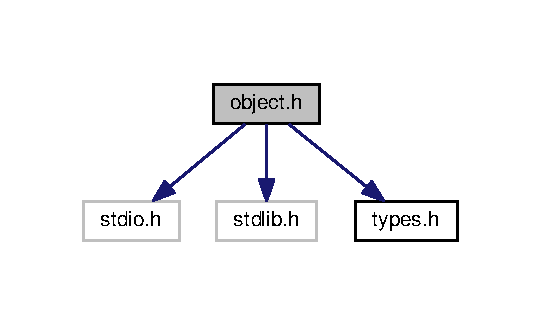
\includegraphics[width=259pt]{object_8h__incl}
\end{center}
\end{figure}
This graph shows which files directly or indirectly include this file\+:\nopagebreak
\begin{figure}[H]
\begin{center}
\leavevmode
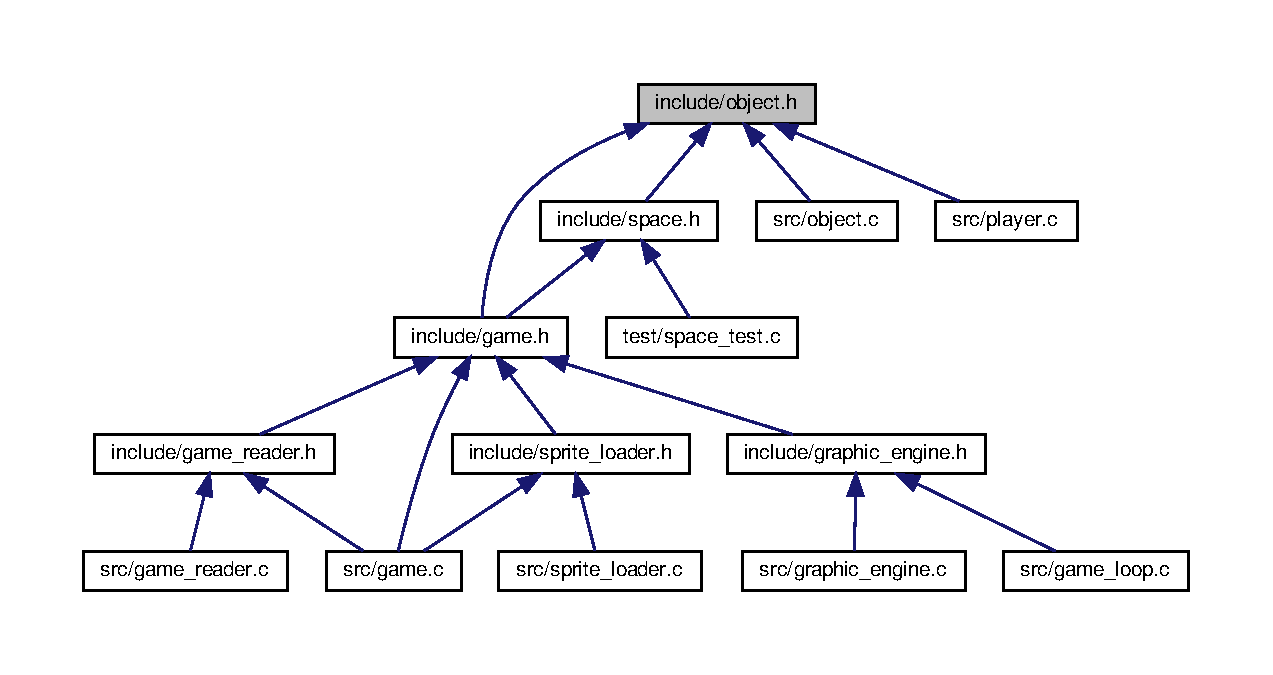
\includegraphics[width=350pt]{object_8h__dep__incl}
\end{center}
\end{figure}
\subsection*{Typedefs}
\begin{DoxyCompactItemize}
\item 
typedef struct \hyperlink{struct__Object}{\+\_\+\+Object} \hyperlink{object_8h_a7f8bbcda919b65ce67f92fba08e0212f}{Object}
\end{DoxyCompactItemize}
\subsection*{Functions}
\begin{DoxyCompactItemize}
\item 
\hyperlink{object_8h_a7f8bbcda919b65ce67f92fba08e0212f}{Object} $\ast$ \hyperlink{object_8h_aa82aed57fe2cd15cdad97c7d706bf72d}{object\+\_\+create} (char $\ast$name, \hyperlink{types_8h_a845e604fb28f7e3d97549da3448149d3}{Id} id, \hyperlink{types_8h_a3e5b8192e7d9ffaf3542f1210aec18dd}{B\+O\+OL} mobile, \hyperlink{types_8h_a3e5b8192e7d9ffaf3542f1210aec18dd}{B\+O\+OL} hidden, \hyperlink{types_8h_a845e604fb28f7e3d97549da3448149d3}{Id} open, \hyperlink{types_8h_a3e5b8192e7d9ffaf3542f1210aec18dd}{B\+O\+OL} lights, \hyperlink{types_8h_a3e5b8192e7d9ffaf3542f1210aec18dd}{B\+O\+OL} on)
\item 
void \hyperlink{object_8h_a355e2f55e8467c2cfb2ef6bd5abbabfb}{object\+\_\+destroy} (\hyperlink{object_8h_a7f8bbcda919b65ce67f92fba08e0212f}{Object} $\ast$obj)
\item 
\hyperlink{types_8h_a32c27cc471df37f4fc818d65de0a56c4}{S\+T\+A\+T\+US} \hyperlink{object_8h_a1f468a3ddebae0cf31431705a824371a}{object\+\_\+set\+\_\+name} (\hyperlink{object_8h_a7f8bbcda919b65ce67f92fba08e0212f}{Object} $\ast$obj, char $\ast$name)
\item 
\hyperlink{types_8h_a32c27cc471df37f4fc818d65de0a56c4}{S\+T\+A\+T\+US} \hyperlink{object_8h_a82b3e96992079f00a8553edd18777ef9}{object\+\_\+set\+\_\+description} (\hyperlink{object_8h_a7f8bbcda919b65ce67f92fba08e0212f}{Object} $\ast$obj, char $\ast$descript)
\item 
\hyperlink{types_8h_a32c27cc471df37f4fc818d65de0a56c4}{S\+T\+A\+T\+US} \hyperlink{object_8h_afcf71b4444a014a542f82c78bc9ee112}{object\+\_\+set\+\_\+id} (\hyperlink{object_8h_a7f8bbcda919b65ce67f92fba08e0212f}{Object} $\ast$obj, \hyperlink{types_8h_a845e604fb28f7e3d97549da3448149d3}{Id} id)
\item 
char $\ast$ \hyperlink{object_8h_ac6f2a9d9a4ed22600839724e8306f750}{object\+\_\+get\+\_\+name} (\hyperlink{object_8h_a7f8bbcda919b65ce67f92fba08e0212f}{Object} $\ast$obj)
\item 
char $\ast$ \hyperlink{object_8h_a42dcce5b32474b5d2500329b97913c15}{object\+\_\+get\+\_\+description} (\hyperlink{object_8h_a7f8bbcda919b65ce67f92fba08e0212f}{Object} $\ast$obj)
\item 
\hyperlink{types_8h_a32c27cc471df37f4fc818d65de0a56c4}{S\+T\+A\+T\+US} \hyperlink{object_8h_ac40dd277ec48ef8b6d9ef5f2a3458c1d}{object\+\_\+description\+\_\+print} (\hyperlink{object_8h_a7f8bbcda919b65ce67f92fba08e0212f}{Object} $\ast$obj, F\+I\+LE $\ast$f)
\item 
\hyperlink{types_8h_a845e604fb28f7e3d97549da3448149d3}{Id} \hyperlink{object_8h_ac9c3ace11b0440f373c67ccd3801398e}{object\+\_\+get\+\_\+id} (\hyperlink{object_8h_a7f8bbcda919b65ce67f92fba08e0212f}{Object} $\ast$obj)
\item 
\hyperlink{types_8h_a3e5b8192e7d9ffaf3542f1210aec18dd}{B\+O\+OL} \hyperlink{object_8h_ab9282b4ff63acf0dcaf27a3d28d3a688}{object\+\_\+get\+\_\+mobile} (\hyperlink{object_8h_a7f8bbcda919b65ce67f92fba08e0212f}{Object} $\ast$obj)
\item 
\hyperlink{types_8h_a32c27cc471df37f4fc818d65de0a56c4}{S\+T\+A\+T\+US} \hyperlink{object_8h_a0aec0c591075ae14b5e939679c2e0c77}{object\+\_\+set\+\_\+mobile} (\hyperlink{object_8h_a7f8bbcda919b65ce67f92fba08e0212f}{Object} $\ast$obj, \hyperlink{types_8h_a3e5b8192e7d9ffaf3542f1210aec18dd}{B\+O\+OL} mobile)
\item 
\hyperlink{types_8h_a3e5b8192e7d9ffaf3542f1210aec18dd}{B\+O\+OL} \hyperlink{object_8h_a46c2c0fff2f0dafb286860f05df9c011}{object\+\_\+get\+\_\+moved} (\hyperlink{object_8h_a7f8bbcda919b65ce67f92fba08e0212f}{Object} $\ast$obj)
\item 
\hyperlink{types_8h_a32c27cc471df37f4fc818d65de0a56c4}{S\+T\+A\+T\+US} \hyperlink{object_8h_a690183bd5b1a2e379d2278d865db65c9}{object\+\_\+set\+\_\+moved} (\hyperlink{object_8h_a7f8bbcda919b65ce67f92fba08e0212f}{Object} $\ast$obj, \hyperlink{types_8h_a3e5b8192e7d9ffaf3542f1210aec18dd}{B\+O\+OL} moved)
\item 
\hyperlink{types_8h_a3e5b8192e7d9ffaf3542f1210aec18dd}{B\+O\+OL} \hyperlink{object_8h_a7d1ff424be4e9977870524af98195d03}{object\+\_\+get\+\_\+hidden} (\hyperlink{object_8h_a7f8bbcda919b65ce67f92fba08e0212f}{Object} $\ast$obj)
\item 
\hyperlink{types_8h_a32c27cc471df37f4fc818d65de0a56c4}{S\+T\+A\+T\+US} \hyperlink{object_8h_ab7ad888deffb05c3ea60a3272045d3e7}{object\+\_\+set\+\_\+hidden} (\hyperlink{object_8h_a7f8bbcda919b65ce67f92fba08e0212f}{Object} $\ast$obj, \hyperlink{types_8h_a3e5b8192e7d9ffaf3542f1210aec18dd}{B\+O\+OL} hidden)
\item 
\hyperlink{types_8h_a3e5b8192e7d9ffaf3542f1210aec18dd}{B\+O\+OL} \hyperlink{object_8h_aa4487278faa32fe5ef8b460fcd7fb51b}{object\+\_\+get\+\_\+iluminati} (\hyperlink{object_8h_a7f8bbcda919b65ce67f92fba08e0212f}{Object} $\ast$obj)
\item 
\hyperlink{types_8h_a32c27cc471df37f4fc818d65de0a56c4}{S\+T\+A\+T\+US} \hyperlink{object_8h_a68bca58bf577e4e6c6d0e730c995f462}{object\+\_\+set\+\_\+ilumnati} (\hyperlink{object_8h_a7f8bbcda919b65ce67f92fba08e0212f}{Object} $\ast$obj, \hyperlink{types_8h_a3e5b8192e7d9ffaf3542f1210aec18dd}{B\+O\+OL} iluminati)
\item 
\hyperlink{types_8h_a845e604fb28f7e3d97549da3448149d3}{Id} \hyperlink{object_8h_a12c50791181c563bae6afa6f7c81edb3}{object\+\_\+get\+\_\+open} (\hyperlink{object_8h_a7f8bbcda919b65ce67f92fba08e0212f}{Object} $\ast$obj)
\item 
\hyperlink{types_8h_a32c27cc471df37f4fc818d65de0a56c4}{S\+T\+A\+T\+US} \hyperlink{object_8h_a43cfcb9c970d34e8a1063b312fdc9d66}{object\+\_\+set\+\_\+open} (\hyperlink{object_8h_a7f8bbcda919b65ce67f92fba08e0212f}{Object} $\ast$obj, \hyperlink{types_8h_a845e604fb28f7e3d97549da3448149d3}{Id} open)
\item 
\hyperlink{types_8h_a3e5b8192e7d9ffaf3542f1210aec18dd}{B\+O\+OL} \hyperlink{object_8h_a474d1a2f46fd4f9a998df134f2b5366c}{object\+\_\+get\+\_\+on} (\hyperlink{object_8h_a7f8bbcda919b65ce67f92fba08e0212f}{Object} $\ast$obj)
\item 
\hyperlink{types_8h_a32c27cc471df37f4fc818d65de0a56c4}{S\+T\+A\+T\+US} \hyperlink{object_8h_af9a46e1a671bf4bbf13520276a4ec941}{object\+\_\+set\+\_\+on} (\hyperlink{object_8h_a7f8bbcda919b65ce67f92fba08e0212f}{Object} $\ast$obj, \hyperlink{types_8h_a3e5b8192e7d9ffaf3542f1210aec18dd}{B\+O\+OL} on)
\item 
char $\ast$ \hyperlink{object_8h_a316c17cfe0a58a3752564561a4a2e5cf}{object\+\_\+get\+\_\+description\+\_\+alternative} (\hyperlink{object_8h_a7f8bbcda919b65ce67f92fba08e0212f}{Object} $\ast$obj)
\item 
\hyperlink{types_8h_a32c27cc471df37f4fc818d65de0a56c4}{S\+T\+A\+T\+US} \hyperlink{object_8h_aa3245ab5de79a33e6ab82ca8e4f93764}{object\+\_\+set\+\_\+description\+\_\+alternative} (\hyperlink{object_8h_a7f8bbcda919b65ce67f92fba08e0212f}{Object} $\ast$obj, char $\ast$description\+\_\+al)
\item 
\hyperlink{types_8h_a32c27cc471df37f4fc818d65de0a56c4}{S\+T\+A\+T\+US} \hyperlink{object_8h_a85d8ceacb9b2c4058cc1a1312a830ad9}{object\+\_\+description\+\_\+al\+\_\+print} (\hyperlink{object_8h_a7f8bbcda919b65ce67f92fba08e0212f}{Object} $\ast$obj, F\+I\+LE $\ast$f)
\end{DoxyCompactItemize}


\subsection{Detailed Description}
Functions for the creation of objects. 

\begin{DoxyAuthor}{Author}
Guillermo R�os 
\end{DoxyAuthor}
\begin{DoxyCopyright}{Copyright}
G\+NU Public License 
\end{DoxyCopyright}


\subsection{Typedef Documentation}
\index{object.\+h@{object.\+h}!Object@{Object}}
\index{Object@{Object}!object.\+h@{object.\+h}}
\subsubsection[{\texorpdfstring{Object}{Object}}]{\setlength{\rightskip}{0pt plus 5cm}typedef struct {\bf \+\_\+\+Object} {\bf Object}}\hypertarget{object_8h_a7f8bbcda919b65ce67f92fba08e0212f}{}\label{object_8h_a7f8bbcda919b65ce67f92fba08e0212f}


\subsection{Function Documentation}
\index{object.\+h@{object.\+h}!object\+\_\+create@{object\+\_\+create}}
\index{object\+\_\+create@{object\+\_\+create}!object.\+h@{object.\+h}}
\subsubsection[{\texorpdfstring{object\+\_\+create(char $\ast$name, Id id, B\+O\+O\+L mobile, B\+O\+O\+L hidden, Id open, B\+O\+O\+L lights, B\+O\+O\+L on)}{object_create(char *name, Id id, BOOL mobile, BOOL hidden, Id open, BOOL lights, BOOL on)}}]{\setlength{\rightskip}{0pt plus 5cm}{\bf Object}$\ast$ object\+\_\+create (
\begin{DoxyParamCaption}
\item[{char $\ast$}]{name, }
\item[{{\bf Id}}]{id, }
\item[{{\bf B\+O\+OL}}]{mobile, }
\item[{{\bf B\+O\+OL}}]{hidden, }
\item[{{\bf Id}}]{open, }
\item[{{\bf B\+O\+OL}}]{lights, }
\item[{{\bf B\+O\+OL}}]{on}
\end{DoxyParamCaption}
)}\hypertarget{object_8h_aa82aed57fe2cd15cdad97c7d706bf72d}{}\label{object_8h_aa82aed57fe2cd15cdad97c7d706bf72d}
\index{object.\+h@{object.\+h}!object\+\_\+description\+\_\+al\+\_\+print@{object\+\_\+description\+\_\+al\+\_\+print}}
\index{object\+\_\+description\+\_\+al\+\_\+print@{object\+\_\+description\+\_\+al\+\_\+print}!object.\+h@{object.\+h}}
\subsubsection[{\texorpdfstring{object\+\_\+description\+\_\+al\+\_\+print(\+Object $\ast$obj, F\+I\+L\+E $\ast$f)}{object_description_al_print(Object *obj, FILE *f)}}]{\setlength{\rightskip}{0pt plus 5cm}{\bf S\+T\+A\+T\+US} object\+\_\+description\+\_\+al\+\_\+print (
\begin{DoxyParamCaption}
\item[{{\bf Object} $\ast$}]{obj, }
\item[{F\+I\+LE $\ast$}]{f}
\end{DoxyParamCaption}
)}\hypertarget{object_8h_a85d8ceacb9b2c4058cc1a1312a830ad9}{}\label{object_8h_a85d8ceacb9b2c4058cc1a1312a830ad9}
\index{object.\+h@{object.\+h}!object\+\_\+description\+\_\+print@{object\+\_\+description\+\_\+print}}
\index{object\+\_\+description\+\_\+print@{object\+\_\+description\+\_\+print}!object.\+h@{object.\+h}}
\subsubsection[{\texorpdfstring{object\+\_\+description\+\_\+print(\+Object $\ast$obj, F\+I\+L\+E $\ast$f)}{object_description_print(Object *obj, FILE *f)}}]{\setlength{\rightskip}{0pt plus 5cm}{\bf S\+T\+A\+T\+US} object\+\_\+description\+\_\+print (
\begin{DoxyParamCaption}
\item[{{\bf Object} $\ast$}]{obj, }
\item[{F\+I\+LE $\ast$}]{f}
\end{DoxyParamCaption}
)}\hypertarget{object_8h_ac40dd277ec48ef8b6d9ef5f2a3458c1d}{}\label{object_8h_ac40dd277ec48ef8b6d9ef5f2a3458c1d}
\index{object.\+h@{object.\+h}!object\+\_\+destroy@{object\+\_\+destroy}}
\index{object\+\_\+destroy@{object\+\_\+destroy}!object.\+h@{object.\+h}}
\subsubsection[{\texorpdfstring{object\+\_\+destroy(\+Object $\ast$obj)}{object_destroy(Object *obj)}}]{\setlength{\rightskip}{0pt plus 5cm}void object\+\_\+destroy (
\begin{DoxyParamCaption}
\item[{{\bf Object} $\ast$}]{obj}
\end{DoxyParamCaption}
)}\hypertarget{object_8h_a355e2f55e8467c2cfb2ef6bd5abbabfb}{}\label{object_8h_a355e2f55e8467c2cfb2ef6bd5abbabfb}
\index{object.\+h@{object.\+h}!object\+\_\+get\+\_\+description@{object\+\_\+get\+\_\+description}}
\index{object\+\_\+get\+\_\+description@{object\+\_\+get\+\_\+description}!object.\+h@{object.\+h}}
\subsubsection[{\texorpdfstring{object\+\_\+get\+\_\+description(\+Object $\ast$obj)}{object_get_description(Object *obj)}}]{\setlength{\rightskip}{0pt plus 5cm}char$\ast$ object\+\_\+get\+\_\+description (
\begin{DoxyParamCaption}
\item[{{\bf Object} $\ast$}]{obj}
\end{DoxyParamCaption}
)}\hypertarget{object_8h_a42dcce5b32474b5d2500329b97913c15}{}\label{object_8h_a42dcce5b32474b5d2500329b97913c15}
\index{object.\+h@{object.\+h}!object\+\_\+get\+\_\+description\+\_\+alternative@{object\+\_\+get\+\_\+description\+\_\+alternative}}
\index{object\+\_\+get\+\_\+description\+\_\+alternative@{object\+\_\+get\+\_\+description\+\_\+alternative}!object.\+h@{object.\+h}}
\subsubsection[{\texorpdfstring{object\+\_\+get\+\_\+description\+\_\+alternative(\+Object $\ast$obj)}{object_get_description_alternative(Object *obj)}}]{\setlength{\rightskip}{0pt plus 5cm}char$\ast$ object\+\_\+get\+\_\+description\+\_\+alternative (
\begin{DoxyParamCaption}
\item[{{\bf Object} $\ast$}]{obj}
\end{DoxyParamCaption}
)}\hypertarget{object_8h_a316c17cfe0a58a3752564561a4a2e5cf}{}\label{object_8h_a316c17cfe0a58a3752564561a4a2e5cf}
\index{object.\+h@{object.\+h}!object\+\_\+get\+\_\+hidden@{object\+\_\+get\+\_\+hidden}}
\index{object\+\_\+get\+\_\+hidden@{object\+\_\+get\+\_\+hidden}!object.\+h@{object.\+h}}
\subsubsection[{\texorpdfstring{object\+\_\+get\+\_\+hidden(\+Object $\ast$obj)}{object_get_hidden(Object *obj)}}]{\setlength{\rightskip}{0pt plus 5cm}{\bf B\+O\+OL} object\+\_\+get\+\_\+hidden (
\begin{DoxyParamCaption}
\item[{{\bf Object} $\ast$}]{obj}
\end{DoxyParamCaption}
)}\hypertarget{object_8h_a7d1ff424be4e9977870524af98195d03}{}\label{object_8h_a7d1ff424be4e9977870524af98195d03}
\index{object.\+h@{object.\+h}!object\+\_\+get\+\_\+id@{object\+\_\+get\+\_\+id}}
\index{object\+\_\+get\+\_\+id@{object\+\_\+get\+\_\+id}!object.\+h@{object.\+h}}
\subsubsection[{\texorpdfstring{object\+\_\+get\+\_\+id(\+Object $\ast$obj)}{object_get_id(Object *obj)}}]{\setlength{\rightskip}{0pt plus 5cm}{\bf Id} object\+\_\+get\+\_\+id (
\begin{DoxyParamCaption}
\item[{{\bf Object} $\ast$}]{obj}
\end{DoxyParamCaption}
)}\hypertarget{object_8h_ac9c3ace11b0440f373c67ccd3801398e}{}\label{object_8h_ac9c3ace11b0440f373c67ccd3801398e}
\index{object.\+h@{object.\+h}!object\+\_\+get\+\_\+iluminati@{object\+\_\+get\+\_\+iluminati}}
\index{object\+\_\+get\+\_\+iluminati@{object\+\_\+get\+\_\+iluminati}!object.\+h@{object.\+h}}
\subsubsection[{\texorpdfstring{object\+\_\+get\+\_\+iluminati(\+Object $\ast$obj)}{object_get_iluminati(Object *obj)}}]{\setlength{\rightskip}{0pt plus 5cm}{\bf B\+O\+OL} object\+\_\+get\+\_\+iluminati (
\begin{DoxyParamCaption}
\item[{{\bf Object} $\ast$}]{obj}
\end{DoxyParamCaption}
)}\hypertarget{object_8h_aa4487278faa32fe5ef8b460fcd7fb51b}{}\label{object_8h_aa4487278faa32fe5ef8b460fcd7fb51b}
\index{object.\+h@{object.\+h}!object\+\_\+get\+\_\+mobile@{object\+\_\+get\+\_\+mobile}}
\index{object\+\_\+get\+\_\+mobile@{object\+\_\+get\+\_\+mobile}!object.\+h@{object.\+h}}
\subsubsection[{\texorpdfstring{object\+\_\+get\+\_\+mobile(\+Object $\ast$obj)}{object_get_mobile(Object *obj)}}]{\setlength{\rightskip}{0pt plus 5cm}{\bf B\+O\+OL} object\+\_\+get\+\_\+mobile (
\begin{DoxyParamCaption}
\item[{{\bf Object} $\ast$}]{obj}
\end{DoxyParamCaption}
)}\hypertarget{object_8h_ab9282b4ff63acf0dcaf27a3d28d3a688}{}\label{object_8h_ab9282b4ff63acf0dcaf27a3d28d3a688}
\index{object.\+h@{object.\+h}!object\+\_\+get\+\_\+moved@{object\+\_\+get\+\_\+moved}}
\index{object\+\_\+get\+\_\+moved@{object\+\_\+get\+\_\+moved}!object.\+h@{object.\+h}}
\subsubsection[{\texorpdfstring{object\+\_\+get\+\_\+moved(\+Object $\ast$obj)}{object_get_moved(Object *obj)}}]{\setlength{\rightskip}{0pt plus 5cm}{\bf B\+O\+OL} object\+\_\+get\+\_\+moved (
\begin{DoxyParamCaption}
\item[{{\bf Object} $\ast$}]{obj}
\end{DoxyParamCaption}
)}\hypertarget{object_8h_a46c2c0fff2f0dafb286860f05df9c011}{}\label{object_8h_a46c2c0fff2f0dafb286860f05df9c011}
\index{object.\+h@{object.\+h}!object\+\_\+get\+\_\+name@{object\+\_\+get\+\_\+name}}
\index{object\+\_\+get\+\_\+name@{object\+\_\+get\+\_\+name}!object.\+h@{object.\+h}}
\subsubsection[{\texorpdfstring{object\+\_\+get\+\_\+name(\+Object $\ast$obj)}{object_get_name(Object *obj)}}]{\setlength{\rightskip}{0pt plus 5cm}char$\ast$ object\+\_\+get\+\_\+name (
\begin{DoxyParamCaption}
\item[{{\bf Object} $\ast$}]{obj}
\end{DoxyParamCaption}
)}\hypertarget{object_8h_ac6f2a9d9a4ed22600839724e8306f750}{}\label{object_8h_ac6f2a9d9a4ed22600839724e8306f750}
\index{object.\+h@{object.\+h}!object\+\_\+get\+\_\+on@{object\+\_\+get\+\_\+on}}
\index{object\+\_\+get\+\_\+on@{object\+\_\+get\+\_\+on}!object.\+h@{object.\+h}}
\subsubsection[{\texorpdfstring{object\+\_\+get\+\_\+on(\+Object $\ast$obj)}{object_get_on(Object *obj)}}]{\setlength{\rightskip}{0pt plus 5cm}{\bf B\+O\+OL} object\+\_\+get\+\_\+on (
\begin{DoxyParamCaption}
\item[{{\bf Object} $\ast$}]{obj}
\end{DoxyParamCaption}
)}\hypertarget{object_8h_a474d1a2f46fd4f9a998df134f2b5366c}{}\label{object_8h_a474d1a2f46fd4f9a998df134f2b5366c}
\index{object.\+h@{object.\+h}!object\+\_\+get\+\_\+open@{object\+\_\+get\+\_\+open}}
\index{object\+\_\+get\+\_\+open@{object\+\_\+get\+\_\+open}!object.\+h@{object.\+h}}
\subsubsection[{\texorpdfstring{object\+\_\+get\+\_\+open(\+Object $\ast$obj)}{object_get_open(Object *obj)}}]{\setlength{\rightskip}{0pt plus 5cm}{\bf Id} object\+\_\+get\+\_\+open (
\begin{DoxyParamCaption}
\item[{{\bf Object} $\ast$}]{obj}
\end{DoxyParamCaption}
)}\hypertarget{object_8h_a12c50791181c563bae6afa6f7c81edb3}{}\label{object_8h_a12c50791181c563bae6afa6f7c81edb3}
\index{object.\+h@{object.\+h}!object\+\_\+set\+\_\+description@{object\+\_\+set\+\_\+description}}
\index{object\+\_\+set\+\_\+description@{object\+\_\+set\+\_\+description}!object.\+h@{object.\+h}}
\subsubsection[{\texorpdfstring{object\+\_\+set\+\_\+description(\+Object $\ast$obj, char $\ast$descript)}{object_set_description(Object *obj, char *descript)}}]{\setlength{\rightskip}{0pt plus 5cm}{\bf S\+T\+A\+T\+US} object\+\_\+set\+\_\+description (
\begin{DoxyParamCaption}
\item[{{\bf Object} $\ast$}]{obj, }
\item[{char $\ast$}]{descript}
\end{DoxyParamCaption}
)}\hypertarget{object_8h_a82b3e96992079f00a8553edd18777ef9}{}\label{object_8h_a82b3e96992079f00a8553edd18777ef9}
\index{object.\+h@{object.\+h}!object\+\_\+set\+\_\+description\+\_\+alternative@{object\+\_\+set\+\_\+description\+\_\+alternative}}
\index{object\+\_\+set\+\_\+description\+\_\+alternative@{object\+\_\+set\+\_\+description\+\_\+alternative}!object.\+h@{object.\+h}}
\subsubsection[{\texorpdfstring{object\+\_\+set\+\_\+description\+\_\+alternative(\+Object $\ast$obj, char $\ast$description\+\_\+al)}{object_set_description_alternative(Object *obj, char *description_al)}}]{\setlength{\rightskip}{0pt plus 5cm}{\bf S\+T\+A\+T\+US} object\+\_\+set\+\_\+description\+\_\+alternative (
\begin{DoxyParamCaption}
\item[{{\bf Object} $\ast$}]{obj, }
\item[{char $\ast$}]{description\+\_\+al}
\end{DoxyParamCaption}
)}\hypertarget{object_8h_aa3245ab5de79a33e6ab82ca8e4f93764}{}\label{object_8h_aa3245ab5de79a33e6ab82ca8e4f93764}
\index{object.\+h@{object.\+h}!object\+\_\+set\+\_\+hidden@{object\+\_\+set\+\_\+hidden}}
\index{object\+\_\+set\+\_\+hidden@{object\+\_\+set\+\_\+hidden}!object.\+h@{object.\+h}}
\subsubsection[{\texorpdfstring{object\+\_\+set\+\_\+hidden(\+Object $\ast$obj, B\+O\+O\+L hidden)}{object_set_hidden(Object *obj, BOOL hidden)}}]{\setlength{\rightskip}{0pt plus 5cm}{\bf S\+T\+A\+T\+US} object\+\_\+set\+\_\+hidden (
\begin{DoxyParamCaption}
\item[{{\bf Object} $\ast$}]{obj, }
\item[{{\bf B\+O\+OL}}]{hidden}
\end{DoxyParamCaption}
)}\hypertarget{object_8h_ab7ad888deffb05c3ea60a3272045d3e7}{}\label{object_8h_ab7ad888deffb05c3ea60a3272045d3e7}
\index{object.\+h@{object.\+h}!object\+\_\+set\+\_\+id@{object\+\_\+set\+\_\+id}}
\index{object\+\_\+set\+\_\+id@{object\+\_\+set\+\_\+id}!object.\+h@{object.\+h}}
\subsubsection[{\texorpdfstring{object\+\_\+set\+\_\+id(\+Object $\ast$obj, Id id)}{object_set_id(Object *obj, Id id)}}]{\setlength{\rightskip}{0pt plus 5cm}{\bf S\+T\+A\+T\+US} object\+\_\+set\+\_\+id (
\begin{DoxyParamCaption}
\item[{{\bf Object} $\ast$}]{obj, }
\item[{{\bf Id}}]{id}
\end{DoxyParamCaption}
)}\hypertarget{object_8h_afcf71b4444a014a542f82c78bc9ee112}{}\label{object_8h_afcf71b4444a014a542f82c78bc9ee112}
\index{object.\+h@{object.\+h}!object\+\_\+set\+\_\+ilumnati@{object\+\_\+set\+\_\+ilumnati}}
\index{object\+\_\+set\+\_\+ilumnati@{object\+\_\+set\+\_\+ilumnati}!object.\+h@{object.\+h}}
\subsubsection[{\texorpdfstring{object\+\_\+set\+\_\+ilumnati(\+Object $\ast$obj, B\+O\+O\+L iluminati)}{object_set_ilumnati(Object *obj, BOOL iluminati)}}]{\setlength{\rightskip}{0pt plus 5cm}{\bf S\+T\+A\+T\+US} object\+\_\+set\+\_\+ilumnati (
\begin{DoxyParamCaption}
\item[{{\bf Object} $\ast$}]{obj, }
\item[{{\bf B\+O\+OL}}]{iluminati}
\end{DoxyParamCaption}
)}\hypertarget{object_8h_a68bca58bf577e4e6c6d0e730c995f462}{}\label{object_8h_a68bca58bf577e4e6c6d0e730c995f462}
\index{object.\+h@{object.\+h}!object\+\_\+set\+\_\+mobile@{object\+\_\+set\+\_\+mobile}}
\index{object\+\_\+set\+\_\+mobile@{object\+\_\+set\+\_\+mobile}!object.\+h@{object.\+h}}
\subsubsection[{\texorpdfstring{object\+\_\+set\+\_\+mobile(\+Object $\ast$obj, B\+O\+O\+L mobile)}{object_set_mobile(Object *obj, BOOL mobile)}}]{\setlength{\rightskip}{0pt plus 5cm}{\bf S\+T\+A\+T\+US} object\+\_\+set\+\_\+mobile (
\begin{DoxyParamCaption}
\item[{{\bf Object} $\ast$}]{obj, }
\item[{{\bf B\+O\+OL}}]{mobile}
\end{DoxyParamCaption}
)}\hypertarget{object_8h_a0aec0c591075ae14b5e939679c2e0c77}{}\label{object_8h_a0aec0c591075ae14b5e939679c2e0c77}
\index{object.\+h@{object.\+h}!object\+\_\+set\+\_\+moved@{object\+\_\+set\+\_\+moved}}
\index{object\+\_\+set\+\_\+moved@{object\+\_\+set\+\_\+moved}!object.\+h@{object.\+h}}
\subsubsection[{\texorpdfstring{object\+\_\+set\+\_\+moved(\+Object $\ast$obj, B\+O\+O\+L moved)}{object_set_moved(Object *obj, BOOL moved)}}]{\setlength{\rightskip}{0pt plus 5cm}{\bf S\+T\+A\+T\+US} object\+\_\+set\+\_\+moved (
\begin{DoxyParamCaption}
\item[{{\bf Object} $\ast$}]{obj, }
\item[{{\bf B\+O\+OL}}]{moved}
\end{DoxyParamCaption}
)}\hypertarget{object_8h_a690183bd5b1a2e379d2278d865db65c9}{}\label{object_8h_a690183bd5b1a2e379d2278d865db65c9}
\index{object.\+h@{object.\+h}!object\+\_\+set\+\_\+name@{object\+\_\+set\+\_\+name}}
\index{object\+\_\+set\+\_\+name@{object\+\_\+set\+\_\+name}!object.\+h@{object.\+h}}
\subsubsection[{\texorpdfstring{object\+\_\+set\+\_\+name(\+Object $\ast$obj, char $\ast$name)}{object_set_name(Object *obj, char *name)}}]{\setlength{\rightskip}{0pt plus 5cm}{\bf S\+T\+A\+T\+US} object\+\_\+set\+\_\+name (
\begin{DoxyParamCaption}
\item[{{\bf Object} $\ast$}]{obj, }
\item[{char $\ast$}]{name}
\end{DoxyParamCaption}
)}\hypertarget{object_8h_a1f468a3ddebae0cf31431705a824371a}{}\label{object_8h_a1f468a3ddebae0cf31431705a824371a}
\index{object.\+h@{object.\+h}!object\+\_\+set\+\_\+on@{object\+\_\+set\+\_\+on}}
\index{object\+\_\+set\+\_\+on@{object\+\_\+set\+\_\+on}!object.\+h@{object.\+h}}
\subsubsection[{\texorpdfstring{object\+\_\+set\+\_\+on(\+Object $\ast$obj, B\+O\+O\+L on)}{object_set_on(Object *obj, BOOL on)}}]{\setlength{\rightskip}{0pt plus 5cm}{\bf S\+T\+A\+T\+US} object\+\_\+set\+\_\+on (
\begin{DoxyParamCaption}
\item[{{\bf Object} $\ast$}]{obj, }
\item[{{\bf B\+O\+OL}}]{on}
\end{DoxyParamCaption}
)}\hypertarget{object_8h_af9a46e1a671bf4bbf13520276a4ec941}{}\label{object_8h_af9a46e1a671bf4bbf13520276a4ec941}
\index{object.\+h@{object.\+h}!object\+\_\+set\+\_\+open@{object\+\_\+set\+\_\+open}}
\index{object\+\_\+set\+\_\+open@{object\+\_\+set\+\_\+open}!object.\+h@{object.\+h}}
\subsubsection[{\texorpdfstring{object\+\_\+set\+\_\+open(\+Object $\ast$obj, Id open)}{object_set_open(Object *obj, Id open)}}]{\setlength{\rightskip}{0pt plus 5cm}{\bf S\+T\+A\+T\+US} object\+\_\+set\+\_\+open (
\begin{DoxyParamCaption}
\item[{{\bf Object} $\ast$}]{obj, }
\item[{{\bf Id}}]{open}
\end{DoxyParamCaption}
)}\hypertarget{object_8h_a43cfcb9c970d34e8a1063b312fdc9d66}{}\label{object_8h_a43cfcb9c970d34e8a1063b312fdc9d66}

\hypertarget{object__test_8c}{}\section{object\+\_\+test.\+c File Reference}
\label{object__test_8c}\index{object\+\_\+test.\+c@{object\+\_\+test.\+c}}
{\ttfamily \#include $<$stdio.\+h$>$}\\*
{\ttfamily \#include $<$stdlib.\+h$>$}\\*
{\ttfamily \#include $<$string.\+h$>$}\\*
{\ttfamily \#include \char`\"{}../include/object.\+h\char`\"{}}\\*
{\ttfamily \#include \char`\"{}../include/object\+\_\+test.\+h\char`\"{}}\\*
{\ttfamily \#include \char`\"{}../include/test.\+h\char`\"{}}\\*
Include dependency graph for object\+\_\+test.\+c\+:\nopagebreak
\begin{figure}[H]
\begin{center}
\leavevmode
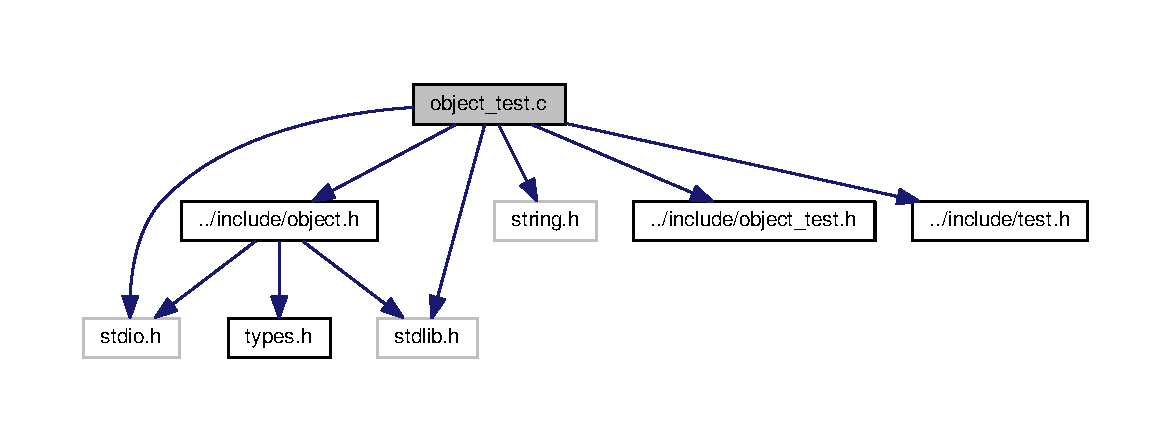
\includegraphics[width=350pt]{object__test_8c__incl}
\end{center}
\end{figure}
\subsection*{Macros}
\begin{DoxyCompactItemize}
\item 
\#define \hyperlink{object__test_8c_a2a77d2f2c5b698c69c19e1f8782bf709}{M\+A\+X\+\_\+\+T\+E\+S\+TS}~28
\end{DoxyCompactItemize}
\subsection*{Functions}
\begin{DoxyCompactItemize}
\item 
int \hyperlink{object__test_8c_a3c04138a5bfe5d72780bb7e82a18e627}{main} (int argc, char $\ast$$\ast$argv)
\begin{DoxyCompactList}\small\item\em Funcion principal de pruebas para el modulo Space. \end{DoxyCompactList}\item 
void \hyperlink{object__test_8c_a3836d69f92ce7149d56bafcaec83f516}{test1\+\_\+object\+\_\+create} ()
\item 
void \hyperlink{object__test_8c_add54ab5e33a1b0a93e9ddcf73591bd9f}{test2\+\_\+object\+\_\+create} ()
\item 
void \hyperlink{object__test_8c_a74e25ad653c4a32b9922fff8e4f916fd}{test1\+\_\+object\+\_\+set\+\_\+name} ()
\item 
void \hyperlink{object__test_8c_acf42b7e7be91ede243f2aaa56c4c9347}{test2\+\_\+object\+\_\+set\+\_\+name} ()
\item 
void \hyperlink{object__test_8c_a6f19ebf6034115c2cdcc3c7bfea25964}{test1\+\_\+object\+\_\+set\+\_\+id} ()
\item 
void \hyperlink{object__test_8c_a1f0cfd69428a6cf954fe37c9c21f8cb3}{test2\+\_\+object\+\_\+set\+\_\+id} ()
\item 
void \hyperlink{object__test_8c_afb26b8c66d332354df8bfd57a8033b8f}{test1\+\_\+object\+\_\+set\+\_\+description} ()
\item 
void \hyperlink{object__test_8c_a65e32c3642c1d9207cdd84b134c616da}{test2\+\_\+object\+\_\+set\+\_\+description} ()
\item 
void \hyperlink{object__test_8c_ad2411bc3cc47c9905e63a3d9c561d369}{test1\+\_\+object\+\_\+get\+\_\+name} ()
\item 
void \hyperlink{object__test_8c_afe180b78a201df7bc1629701db1d464c}{test1\+\_\+object\+\_\+get\+\_\+description} ()
\item 
void \hyperlink{object__test_8c_aa88e9e9dab92ba9c58851d7a7a8415f0}{test1\+\_\+object\+\_\+get\+\_\+id} ()
\end{DoxyCompactItemize}


\subsection{Macro Definition Documentation}
\index{object\+\_\+test.\+c@{object\+\_\+test.\+c}!M\+A\+X\+\_\+\+T\+E\+S\+TS@{M\+A\+X\+\_\+\+T\+E\+S\+TS}}
\index{M\+A\+X\+\_\+\+T\+E\+S\+TS@{M\+A\+X\+\_\+\+T\+E\+S\+TS}!object\+\_\+test.\+c@{object\+\_\+test.\+c}}
\subsubsection[{\texorpdfstring{M\+A\+X\+\_\+\+T\+E\+S\+TS}{MAX_TESTS}}]{\setlength{\rightskip}{0pt plus 5cm}\#define M\+A\+X\+\_\+\+T\+E\+S\+TS~28}\hypertarget{object__test_8c_a2a77d2f2c5b698c69c19e1f8782bf709}{}\label{object__test_8c_a2a77d2f2c5b698c69c19e1f8782bf709}


\subsection{Function Documentation}
\index{object\+\_\+test.\+c@{object\+\_\+test.\+c}!main@{main}}
\index{main@{main}!object\+\_\+test.\+c@{object\+\_\+test.\+c}}
\subsubsection[{\texorpdfstring{main(int argc, char $\ast$$\ast$argv)}{main(int argc, char **argv)}}]{\setlength{\rightskip}{0pt plus 5cm}int main (
\begin{DoxyParamCaption}
\item[{int}]{argc, }
\item[{char $\ast$$\ast$}]{argv}
\end{DoxyParamCaption}
)}\hypertarget{object__test_8c_a3c04138a5bfe5d72780bb7e82a18e627}{}\label{object__test_8c_a3c04138a5bfe5d72780bb7e82a18e627}


Funcion principal de pruebas para el modulo Space. 

Dos modos de ejecucion\+: 1.-\/\+Si se ejecuta sin parametros se ejecutan todas las pruebas 2.-\/\+Si se ejecuta con un numero entre 1 y el numero de pruebas solo ejecuta la prueba indicada \index{object\+\_\+test.\+c@{object\+\_\+test.\+c}!test1\+\_\+object\+\_\+create@{test1\+\_\+object\+\_\+create}}
\index{test1\+\_\+object\+\_\+create@{test1\+\_\+object\+\_\+create}!object\+\_\+test.\+c@{object\+\_\+test.\+c}}
\subsubsection[{\texorpdfstring{test1\+\_\+object\+\_\+create()}{test1_object_create()}}]{\setlength{\rightskip}{0pt plus 5cm}void test1\+\_\+object\+\_\+create (
\begin{DoxyParamCaption}
{}
\end{DoxyParamCaption}
)}\hypertarget{object__test_8c_a3836d69f92ce7149d56bafcaec83f516}{}\label{object__test_8c_a3836d69f92ce7149d56bafcaec83f516}
\index{object\+\_\+test.\+c@{object\+\_\+test.\+c}!test1\+\_\+object\+\_\+get\+\_\+description@{test1\+\_\+object\+\_\+get\+\_\+description}}
\index{test1\+\_\+object\+\_\+get\+\_\+description@{test1\+\_\+object\+\_\+get\+\_\+description}!object\+\_\+test.\+c@{object\+\_\+test.\+c}}
\subsubsection[{\texorpdfstring{test1\+\_\+object\+\_\+get\+\_\+description()}{test1_object_get_description()}}]{\setlength{\rightskip}{0pt plus 5cm}void test1\+\_\+object\+\_\+get\+\_\+description (
\begin{DoxyParamCaption}
{}
\end{DoxyParamCaption}
)}\hypertarget{object__test_8c_afe180b78a201df7bc1629701db1d464c}{}\label{object__test_8c_afe180b78a201df7bc1629701db1d464c}
\index{object\+\_\+test.\+c@{object\+\_\+test.\+c}!test1\+\_\+object\+\_\+get\+\_\+id@{test1\+\_\+object\+\_\+get\+\_\+id}}
\index{test1\+\_\+object\+\_\+get\+\_\+id@{test1\+\_\+object\+\_\+get\+\_\+id}!object\+\_\+test.\+c@{object\+\_\+test.\+c}}
\subsubsection[{\texorpdfstring{test1\+\_\+object\+\_\+get\+\_\+id()}{test1_object_get_id()}}]{\setlength{\rightskip}{0pt plus 5cm}void test1\+\_\+object\+\_\+get\+\_\+id (
\begin{DoxyParamCaption}
{}
\end{DoxyParamCaption}
)}\hypertarget{object__test_8c_aa88e9e9dab92ba9c58851d7a7a8415f0}{}\label{object__test_8c_aa88e9e9dab92ba9c58851d7a7a8415f0}
\index{object\+\_\+test.\+c@{object\+\_\+test.\+c}!test1\+\_\+object\+\_\+get\+\_\+name@{test1\+\_\+object\+\_\+get\+\_\+name}}
\index{test1\+\_\+object\+\_\+get\+\_\+name@{test1\+\_\+object\+\_\+get\+\_\+name}!object\+\_\+test.\+c@{object\+\_\+test.\+c}}
\subsubsection[{\texorpdfstring{test1\+\_\+object\+\_\+get\+\_\+name()}{test1_object_get_name()}}]{\setlength{\rightskip}{0pt plus 5cm}void test1\+\_\+object\+\_\+get\+\_\+name (
\begin{DoxyParamCaption}
{}
\end{DoxyParamCaption}
)}\hypertarget{object__test_8c_ad2411bc3cc47c9905e63a3d9c561d369}{}\label{object__test_8c_ad2411bc3cc47c9905e63a3d9c561d369}
\index{object\+\_\+test.\+c@{object\+\_\+test.\+c}!test1\+\_\+object\+\_\+set\+\_\+description@{test1\+\_\+object\+\_\+set\+\_\+description}}
\index{test1\+\_\+object\+\_\+set\+\_\+description@{test1\+\_\+object\+\_\+set\+\_\+description}!object\+\_\+test.\+c@{object\+\_\+test.\+c}}
\subsubsection[{\texorpdfstring{test1\+\_\+object\+\_\+set\+\_\+description()}{test1_object_set_description()}}]{\setlength{\rightskip}{0pt plus 5cm}void test1\+\_\+object\+\_\+set\+\_\+description (
\begin{DoxyParamCaption}
{}
\end{DoxyParamCaption}
)}\hypertarget{object__test_8c_afb26b8c66d332354df8bfd57a8033b8f}{}\label{object__test_8c_afb26b8c66d332354df8bfd57a8033b8f}
\index{object\+\_\+test.\+c@{object\+\_\+test.\+c}!test1\+\_\+object\+\_\+set\+\_\+id@{test1\+\_\+object\+\_\+set\+\_\+id}}
\index{test1\+\_\+object\+\_\+set\+\_\+id@{test1\+\_\+object\+\_\+set\+\_\+id}!object\+\_\+test.\+c@{object\+\_\+test.\+c}}
\subsubsection[{\texorpdfstring{test1\+\_\+object\+\_\+set\+\_\+id()}{test1_object_set_id()}}]{\setlength{\rightskip}{0pt plus 5cm}void test1\+\_\+object\+\_\+set\+\_\+id (
\begin{DoxyParamCaption}
{}
\end{DoxyParamCaption}
)}\hypertarget{object__test_8c_a6f19ebf6034115c2cdcc3c7bfea25964}{}\label{object__test_8c_a6f19ebf6034115c2cdcc3c7bfea25964}
\index{object\+\_\+test.\+c@{object\+\_\+test.\+c}!test1\+\_\+object\+\_\+set\+\_\+name@{test1\+\_\+object\+\_\+set\+\_\+name}}
\index{test1\+\_\+object\+\_\+set\+\_\+name@{test1\+\_\+object\+\_\+set\+\_\+name}!object\+\_\+test.\+c@{object\+\_\+test.\+c}}
\subsubsection[{\texorpdfstring{test1\+\_\+object\+\_\+set\+\_\+name()}{test1_object_set_name()}}]{\setlength{\rightskip}{0pt plus 5cm}void test1\+\_\+object\+\_\+set\+\_\+name (
\begin{DoxyParamCaption}
{}
\end{DoxyParamCaption}
)}\hypertarget{object__test_8c_a74e25ad653c4a32b9922fff8e4f916fd}{}\label{object__test_8c_a74e25ad653c4a32b9922fff8e4f916fd}
\index{object\+\_\+test.\+c@{object\+\_\+test.\+c}!test2\+\_\+object\+\_\+create@{test2\+\_\+object\+\_\+create}}
\index{test2\+\_\+object\+\_\+create@{test2\+\_\+object\+\_\+create}!object\+\_\+test.\+c@{object\+\_\+test.\+c}}
\subsubsection[{\texorpdfstring{test2\+\_\+object\+\_\+create()}{test2_object_create()}}]{\setlength{\rightskip}{0pt plus 5cm}void test2\+\_\+object\+\_\+create (
\begin{DoxyParamCaption}
{}
\end{DoxyParamCaption}
)}\hypertarget{object__test_8c_add54ab5e33a1b0a93e9ddcf73591bd9f}{}\label{object__test_8c_add54ab5e33a1b0a93e9ddcf73591bd9f}
\index{object\+\_\+test.\+c@{object\+\_\+test.\+c}!test2\+\_\+object\+\_\+set\+\_\+description@{test2\+\_\+object\+\_\+set\+\_\+description}}
\index{test2\+\_\+object\+\_\+set\+\_\+description@{test2\+\_\+object\+\_\+set\+\_\+description}!object\+\_\+test.\+c@{object\+\_\+test.\+c}}
\subsubsection[{\texorpdfstring{test2\+\_\+object\+\_\+set\+\_\+description()}{test2_object_set_description()}}]{\setlength{\rightskip}{0pt plus 5cm}void test2\+\_\+object\+\_\+set\+\_\+description (
\begin{DoxyParamCaption}
{}
\end{DoxyParamCaption}
)}\hypertarget{object__test_8c_a65e32c3642c1d9207cdd84b134c616da}{}\label{object__test_8c_a65e32c3642c1d9207cdd84b134c616da}
\index{object\+\_\+test.\+c@{object\+\_\+test.\+c}!test2\+\_\+object\+\_\+set\+\_\+id@{test2\+\_\+object\+\_\+set\+\_\+id}}
\index{test2\+\_\+object\+\_\+set\+\_\+id@{test2\+\_\+object\+\_\+set\+\_\+id}!object\+\_\+test.\+c@{object\+\_\+test.\+c}}
\subsubsection[{\texorpdfstring{test2\+\_\+object\+\_\+set\+\_\+id()}{test2_object_set_id()}}]{\setlength{\rightskip}{0pt plus 5cm}void test2\+\_\+object\+\_\+set\+\_\+id (
\begin{DoxyParamCaption}
{}
\end{DoxyParamCaption}
)}\hypertarget{object__test_8c_a1f0cfd69428a6cf954fe37c9c21f8cb3}{}\label{object__test_8c_a1f0cfd69428a6cf954fe37c9c21f8cb3}
\index{object\+\_\+test.\+c@{object\+\_\+test.\+c}!test2\+\_\+object\+\_\+set\+\_\+name@{test2\+\_\+object\+\_\+set\+\_\+name}}
\index{test2\+\_\+object\+\_\+set\+\_\+name@{test2\+\_\+object\+\_\+set\+\_\+name}!object\+\_\+test.\+c@{object\+\_\+test.\+c}}
\subsubsection[{\texorpdfstring{test2\+\_\+object\+\_\+set\+\_\+name()}{test2_object_set_name()}}]{\setlength{\rightskip}{0pt plus 5cm}void test2\+\_\+object\+\_\+set\+\_\+name (
\begin{DoxyParamCaption}
{}
\end{DoxyParamCaption}
)}\hypertarget{object__test_8c_acf42b7e7be91ede243f2aaa56c4c9347}{}\label{object__test_8c_acf42b7e7be91ede243f2aaa56c4c9347}

\hypertarget{object__test_8h}{}\section{include/object\+\_\+test.h File Reference}
\label{object__test_8h}\index{include/object\+\_\+test.\+h@{include/object\+\_\+test.\+h}}


It declares the tests for the object module.  


\subsection*{Functions}
\begin{DoxyCompactItemize}
\item 
\mbox{\Hypertarget{object__test_8h_a3836d69f92ce7149d56bafcaec83f516}\label{object__test_8h_a3836d69f92ce7149d56bafcaec83f516}} 
void {\bfseries test1\+\_\+object\+\_\+create} ()
\item 
\mbox{\Hypertarget{object__test_8h_add54ab5e33a1b0a93e9ddcf73591bd9f}\label{object__test_8h_add54ab5e33a1b0a93e9ddcf73591bd9f}} 
void {\bfseries test2\+\_\+object\+\_\+create} ()
\item 
\mbox{\Hypertarget{object__test_8h_a74e25ad653c4a32b9922fff8e4f916fd}\label{object__test_8h_a74e25ad653c4a32b9922fff8e4f916fd}} 
void {\bfseries test1\+\_\+object\+\_\+set\+\_\+name} ()
\item 
\mbox{\Hypertarget{object__test_8h_acf42b7e7be91ede243f2aaa56c4c9347}\label{object__test_8h_acf42b7e7be91ede243f2aaa56c4c9347}} 
void {\bfseries test2\+\_\+object\+\_\+set\+\_\+name} ()
\item 
\mbox{\Hypertarget{object__test_8h_a6f19ebf6034115c2cdcc3c7bfea25964}\label{object__test_8h_a6f19ebf6034115c2cdcc3c7bfea25964}} 
void {\bfseries test1\+\_\+object\+\_\+set\+\_\+id} ()
\item 
\mbox{\Hypertarget{object__test_8h_a1f0cfd69428a6cf954fe37c9c21f8cb3}\label{object__test_8h_a1f0cfd69428a6cf954fe37c9c21f8cb3}} 
void {\bfseries test2\+\_\+object\+\_\+set\+\_\+id} ()
\item 
\mbox{\Hypertarget{object__test_8h_afb26b8c66d332354df8bfd57a8033b8f}\label{object__test_8h_afb26b8c66d332354df8bfd57a8033b8f}} 
void {\bfseries test1\+\_\+object\+\_\+set\+\_\+description} ()
\item 
\mbox{\Hypertarget{object__test_8h_a65e32c3642c1d9207cdd84b134c616da}\label{object__test_8h_a65e32c3642c1d9207cdd84b134c616da}} 
void {\bfseries test2\+\_\+object\+\_\+set\+\_\+description} ()
\item 
\mbox{\Hypertarget{object__test_8h_ad2411bc3cc47c9905e63a3d9c561d369}\label{object__test_8h_ad2411bc3cc47c9905e63a3d9c561d369}} 
void {\bfseries test1\+\_\+object\+\_\+get\+\_\+name} ()
\item 
\mbox{\Hypertarget{object__test_8h_afe180b78a201df7bc1629701db1d464c}\label{object__test_8h_afe180b78a201df7bc1629701db1d464c}} 
void {\bfseries test1\+\_\+object\+\_\+get\+\_\+description} ()
\item 
\mbox{\Hypertarget{object__test_8h_aa88e9e9dab92ba9c58851d7a7a8415f0}\label{object__test_8h_aa88e9e9dab92ba9c58851d7a7a8415f0}} 
void {\bfseries test1\+\_\+object\+\_\+get\+\_\+id} ()
\end{DoxyCompactItemize}


\subsection{Detailed Description}
It declares the tests for the object module. 

\begin{DoxyAuthor}{Author}
Pablo Sánchez 
\end{DoxyAuthor}
\begin{DoxyCopyright}{Copyright}
G\+NU Public License 
\end{DoxyCopyright}

\hypertarget{Objectives__Tracker_8txt}{}\section{Objectives\+\_\+\+Tracker.\+txt File Reference}
\label{Objectives__Tracker_8txt}\index{Objectives\+\_\+\+Tracker.\+txt@{Objectives\+\_\+\+Tracker.\+txt}}

\hypertarget{player_8c}{\section{player.\+c File Reference}
\label{player_8c}\index{player.\+c@{player.\+c}}
}


Functions for the creation of players.  


{\ttfamily \#include $<$string.\+h$>$}\\*
{\ttfamily \#include \char`\"{}../include/player.\+h\char`\"{}}\\*
{\ttfamily \#include \char`\"{}../include/object.\+h\char`\"{}}\\*
{\ttfamily \#include \char`\"{}../include/set.\+h\char`\"{}}\\*
{\ttfamily \#include \char`\"{}../include/inventory.\+h\char`\"{}}\\*
Include dependency graph for player.\+c\+:\nopagebreak
\begin{figure}[H]
\begin{center}
\leavevmode
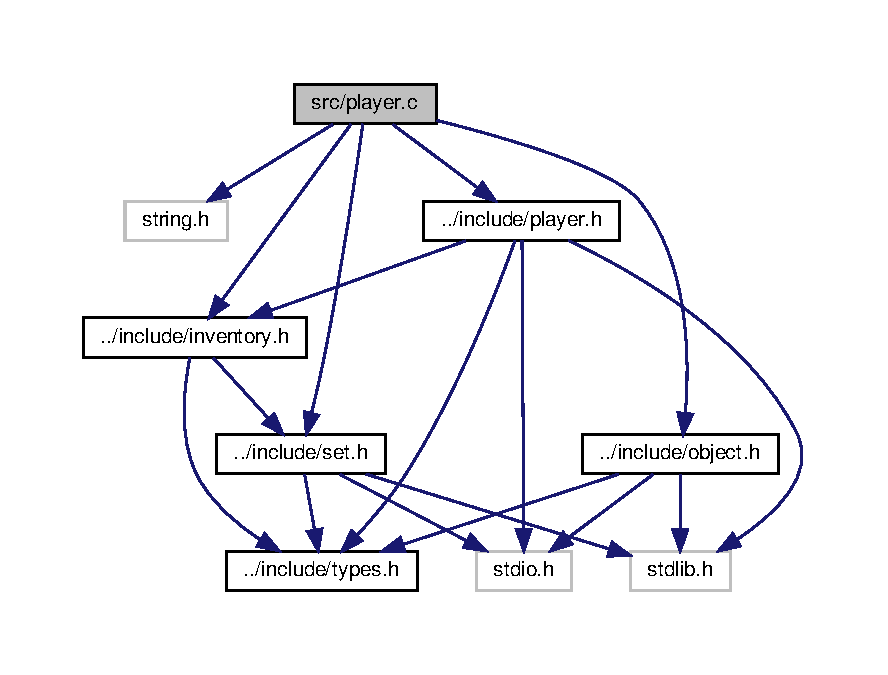
\includegraphics[width=350pt]{player_8c__incl}
\end{center}
\end{figure}
\subsection*{Classes}
\begin{DoxyCompactItemize}
\item 
struct \hyperlink{struct__Player}{\+\_\+\+Player}
\end{DoxyCompactItemize}
\subsection*{Functions}
\begin{DoxyCompactItemize}
\item 
\hyperlink{player_8h_af30e2030635a69690f85e48bc6ef202f}{Player} $\ast$ \hyperlink{player_8c_a875d0de3a82ea2482f7af6fc19ff1b5b}{player\+\_\+create} (char $\ast$name, \hyperlink{types_8h_a845e604fb28f7e3d97549da3448149d3}{Id} location\+\_\+id, \hyperlink{types_8h_a845e604fb28f7e3d97549da3448149d3}{Id} object\+\_\+id, \hyperlink{types_8h_a845e604fb28f7e3d97549da3448149d3}{Id} id)
\item 
void \hyperlink{player_8c_a73b5e14b9a3b1d4111ea2713d666bdc9}{player\+\_\+destroy} (\hyperlink{player_8h_af30e2030635a69690f85e48bc6ef202f}{Player} $\ast$player)
\item 
\hyperlink{types_8h_a32c27cc471df37f4fc818d65de0a56c4}{S\+T\+A\+T\+U\+S} \hyperlink{player_8c_a90fc386643bb025cdcbfa828fe6671e6}{player\+\_\+set\+Name} (\hyperlink{player_8h_af30e2030635a69690f85e48bc6ef202f}{Player} $\ast$player, char $\ast$new\+Name)
\item 
\hyperlink{types_8h_a32c27cc471df37f4fc818d65de0a56c4}{S\+T\+A\+T\+U\+S} \hyperlink{player_8c_a2bc8692e4e6773613c61ebef465935ee}{player\+\_\+set\+Loc\+Id} (\hyperlink{player_8h_af30e2030635a69690f85e48bc6ef202f}{Player} $\ast$player, \hyperlink{types_8h_a845e604fb28f7e3d97549da3448149d3}{Id} new\+\_\+loc\+Id)
\item 
\hyperlink{types_8h_a32c27cc471df37f4fc818d65de0a56c4}{S\+T\+A\+T\+U\+S} \hyperlink{player_8c_a05d8f2a3c866c0eb98246a0ccd7d94de}{player\+\_\+set\+Obj\+Id} (\hyperlink{player_8h_af30e2030635a69690f85e48bc6ef202f}{Player} $\ast$player, \hyperlink{types_8h_a845e604fb28f7e3d97549da3448149d3}{Id} new\+\_\+obj\+Id)
\item 
\hyperlink{types_8h_a32c27cc471df37f4fc818d65de0a56c4}{S\+T\+A\+T\+U\+S} \hyperlink{player_8c_a9ba44a6fe4c38cb50f19e2f0f93bdc18}{player\+\_\+set\+Id} (\hyperlink{player_8h_af30e2030635a69690f85e48bc6ef202f}{Player} $\ast$player, \hyperlink{types_8h_a845e604fb28f7e3d97549da3448149d3}{Id} new\+\_\+id)
\item 
char $\ast$ \hyperlink{player_8c_abdba41f9b63b037f2138068da96ee9bd}{player\+\_\+get\+Name} (\hyperlink{player_8h_af30e2030635a69690f85e48bc6ef202f}{Player} $\ast$player)
\item 
\hyperlink{types_8h_a845e604fb28f7e3d97549da3448149d3}{Id} \hyperlink{player_8c_a0dff36ebf92bedde82a5d60d96072daf}{player\+\_\+get\+Loc\+Id} (\hyperlink{player_8h_af30e2030635a69690f85e48bc6ef202f}{Player} $\ast$player)
\item 
\hyperlink{types_8h_a845e604fb28f7e3d97549da3448149d3}{Id} \hyperlink{player_8c_ac3d514b13a8989a408a6c711ddac0e25}{player\+\_\+get\+Obj\+Id} (\hyperlink{player_8h_af30e2030635a69690f85e48bc6ef202f}{Player} $\ast$player, int num)
\item 
\hyperlink{types_8h_a845e604fb28f7e3d97549da3448149d3}{Id} \hyperlink{player_8c_ac276800d65514e07ad63008b40281442}{player\+\_\+get\+Id} (\hyperlink{player_8h_af30e2030635a69690f85e48bc6ef202f}{Player} $\ast$player)
\item 
\hyperlink{types_8h_a32c27cc471df37f4fc818d65de0a56c4}{S\+T\+A\+T\+U\+S} \hyperlink{player_8c_af618dc361f91ec6678dacca975325c50}{player\+\_\+remove\+Obj\+Id} (\hyperlink{player_8h_af30e2030635a69690f85e48bc6ef202f}{Player} $\ast$player, \hyperlink{types_8h_a845e604fb28f7e3d97549da3448149d3}{Id} id)
\end{DoxyCompactItemize}


\subsection{Detailed Description}
Functions for the creation of players. 

\begin{DoxyAuthor}{Author}
Antonio Solana 
\end{DoxyAuthor}
\begin{DoxyCopyright}{Copyright}
G\+N\+U Public License 
\end{DoxyCopyright}


\subsection{Function Documentation}
\hypertarget{player_8c_a875d0de3a82ea2482f7af6fc19ff1b5b}{\index{player.\+c@{player.\+c}!player\+\_\+create@{player\+\_\+create}}
\index{player\+\_\+create@{player\+\_\+create}!player.\+c@{player.\+c}}
\subsubsection[{player\+\_\+create}]{\setlength{\rightskip}{0pt plus 5cm}{\bf Player}$\ast$ player\+\_\+create (
\begin{DoxyParamCaption}
\item[{char $\ast$}]{name, }
\item[{{\bf Id}}]{location\+\_\+id, }
\item[{{\bf Id}}]{object\+\_\+id, }
\item[{{\bf Id}}]{id}
\end{DoxyParamCaption}
)}}\label{player_8c_a875d0de3a82ea2482f7af6fc19ff1b5b}
Returns null if no name is given to the player Returns pointer to the newly created player if ok\hypertarget{player_8c_a73b5e14b9a3b1d4111ea2713d666bdc9}{\index{player.\+c@{player.\+c}!player\+\_\+destroy@{player\+\_\+destroy}}
\index{player\+\_\+destroy@{player\+\_\+destroy}!player.\+c@{player.\+c}}
\subsubsection[{player\+\_\+destroy}]{\setlength{\rightskip}{0pt plus 5cm}void player\+\_\+destroy (
\begin{DoxyParamCaption}
\item[{{\bf Player} $\ast$}]{player}
\end{DoxyParamCaption}
)}}\label{player_8c_a73b5e14b9a3b1d4111ea2713d666bdc9}
\hypertarget{player_8c_ac276800d65514e07ad63008b40281442}{\index{player.\+c@{player.\+c}!player\+\_\+get\+Id@{player\+\_\+get\+Id}}
\index{player\+\_\+get\+Id@{player\+\_\+get\+Id}!player.\+c@{player.\+c}}
\subsubsection[{player\+\_\+get\+Id}]{\setlength{\rightskip}{0pt plus 5cm}{\bf Id} player\+\_\+get\+Id (
\begin{DoxyParamCaption}
\item[{{\bf Player} $\ast$}]{player}
\end{DoxyParamCaption}
)}}\label{player_8c_ac276800d65514e07ad63008b40281442}
\hypertarget{player_8c_a0dff36ebf92bedde82a5d60d96072daf}{\index{player.\+c@{player.\+c}!player\+\_\+get\+Loc\+Id@{player\+\_\+get\+Loc\+Id}}
\index{player\+\_\+get\+Loc\+Id@{player\+\_\+get\+Loc\+Id}!player.\+c@{player.\+c}}
\subsubsection[{player\+\_\+get\+Loc\+Id}]{\setlength{\rightskip}{0pt plus 5cm}{\bf Id} player\+\_\+get\+Loc\+Id (
\begin{DoxyParamCaption}
\item[{{\bf Player} $\ast$}]{player}
\end{DoxyParamCaption}
)}}\label{player_8c_a0dff36ebf92bedde82a5d60d96072daf}
\hypertarget{player_8c_abdba41f9b63b037f2138068da96ee9bd}{\index{player.\+c@{player.\+c}!player\+\_\+get\+Name@{player\+\_\+get\+Name}}
\index{player\+\_\+get\+Name@{player\+\_\+get\+Name}!player.\+c@{player.\+c}}
\subsubsection[{player\+\_\+get\+Name}]{\setlength{\rightskip}{0pt plus 5cm}char$\ast$ player\+\_\+get\+Name (
\begin{DoxyParamCaption}
\item[{{\bf Player} $\ast$}]{player}
\end{DoxyParamCaption}
)}}\label{player_8c_abdba41f9b63b037f2138068da96ee9bd}
\hypertarget{player_8c_ac3d514b13a8989a408a6c711ddac0e25}{\index{player.\+c@{player.\+c}!player\+\_\+get\+Obj\+Id@{player\+\_\+get\+Obj\+Id}}
\index{player\+\_\+get\+Obj\+Id@{player\+\_\+get\+Obj\+Id}!player.\+c@{player.\+c}}
\subsubsection[{player\+\_\+get\+Obj\+Id}]{\setlength{\rightskip}{0pt plus 5cm}{\bf Id} player\+\_\+get\+Obj\+Id (
\begin{DoxyParamCaption}
\item[{{\bf Player} $\ast$}]{player, }
\item[{int}]{num}
\end{DoxyParamCaption}
)}}\label{player_8c_ac3d514b13a8989a408a6c711ddac0e25}
\hypertarget{player_8c_af618dc361f91ec6678dacca975325c50}{\index{player.\+c@{player.\+c}!player\+\_\+remove\+Obj\+Id@{player\+\_\+remove\+Obj\+Id}}
\index{player\+\_\+remove\+Obj\+Id@{player\+\_\+remove\+Obj\+Id}!player.\+c@{player.\+c}}
\subsubsection[{player\+\_\+remove\+Obj\+Id}]{\setlength{\rightskip}{0pt plus 5cm}{\bf S\+T\+A\+T\+U\+S} player\+\_\+remove\+Obj\+Id (
\begin{DoxyParamCaption}
\item[{{\bf Player} $\ast$}]{player, }
\item[{{\bf Id}}]{id}
\end{DoxyParamCaption}
)}}\label{player_8c_af618dc361f91ec6678dacca975325c50}
\hypertarget{player_8c_a9ba44a6fe4c38cb50f19e2f0f93bdc18}{\index{player.\+c@{player.\+c}!player\+\_\+set\+Id@{player\+\_\+set\+Id}}
\index{player\+\_\+set\+Id@{player\+\_\+set\+Id}!player.\+c@{player.\+c}}
\subsubsection[{player\+\_\+set\+Id}]{\setlength{\rightskip}{0pt plus 5cm}{\bf S\+T\+A\+T\+U\+S} player\+\_\+set\+Id (
\begin{DoxyParamCaption}
\item[{{\bf Player} $\ast$}]{player, }
\item[{{\bf Id}}]{new\+\_\+id}
\end{DoxyParamCaption}
)}}\label{player_8c_a9ba44a6fe4c38cb50f19e2f0f93bdc18}
\hypertarget{player_8c_a2bc8692e4e6773613c61ebef465935ee}{\index{player.\+c@{player.\+c}!player\+\_\+set\+Loc\+Id@{player\+\_\+set\+Loc\+Id}}
\index{player\+\_\+set\+Loc\+Id@{player\+\_\+set\+Loc\+Id}!player.\+c@{player.\+c}}
\subsubsection[{player\+\_\+set\+Loc\+Id}]{\setlength{\rightskip}{0pt plus 5cm}{\bf S\+T\+A\+T\+U\+S} player\+\_\+set\+Loc\+Id (
\begin{DoxyParamCaption}
\item[{{\bf Player} $\ast$}]{player, }
\item[{{\bf Id}}]{new\+\_\+loc\+Id}
\end{DoxyParamCaption}
)}}\label{player_8c_a2bc8692e4e6773613c61ebef465935ee}
\hypertarget{player_8c_a90fc386643bb025cdcbfa828fe6671e6}{\index{player.\+c@{player.\+c}!player\+\_\+set\+Name@{player\+\_\+set\+Name}}
\index{player\+\_\+set\+Name@{player\+\_\+set\+Name}!player.\+c@{player.\+c}}
\subsubsection[{player\+\_\+set\+Name}]{\setlength{\rightskip}{0pt plus 5cm}{\bf S\+T\+A\+T\+U\+S} player\+\_\+set\+Name (
\begin{DoxyParamCaption}
\item[{{\bf Player} $\ast$}]{player, }
\item[{char $\ast$}]{new\+Name}
\end{DoxyParamCaption}
)}}\label{player_8c_a90fc386643bb025cdcbfa828fe6671e6}
\hypertarget{player_8c_a05d8f2a3c866c0eb98246a0ccd7d94de}{\index{player.\+c@{player.\+c}!player\+\_\+set\+Obj\+Id@{player\+\_\+set\+Obj\+Id}}
\index{player\+\_\+set\+Obj\+Id@{player\+\_\+set\+Obj\+Id}!player.\+c@{player.\+c}}
\subsubsection[{player\+\_\+set\+Obj\+Id}]{\setlength{\rightskip}{0pt plus 5cm}{\bf S\+T\+A\+T\+U\+S} player\+\_\+set\+Obj\+Id (
\begin{DoxyParamCaption}
\item[{{\bf Player} $\ast$}]{player, }
\item[{{\bf Id}}]{new\+\_\+obj\+Id}
\end{DoxyParamCaption}
)}}\label{player_8c_a05d8f2a3c866c0eb98246a0ccd7d94de}

\hypertarget{player_8h}{}\section{player.\+h File Reference}
\label{player_8h}\index{player.\+h@{player.\+h}}


Functions for the creation of players.  


{\ttfamily \#include $<$stdio.\+h$>$}\\*
{\ttfamily \#include $<$stdlib.\+h$>$}\\*
{\ttfamily \#include \char`\"{}types.\+h\char`\"{}}\\*
Include dependency graph for player.\+h\+:\nopagebreak
\begin{figure}[H]
\begin{center}
\leavevmode
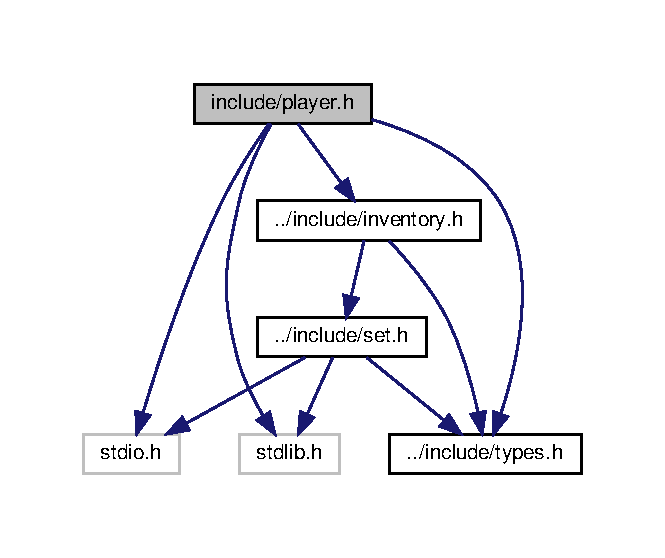
\includegraphics[width=259pt]{player_8h__incl}
\end{center}
\end{figure}
This graph shows which files directly or indirectly include this file\+:\nopagebreak
\begin{figure}[H]
\begin{center}
\leavevmode
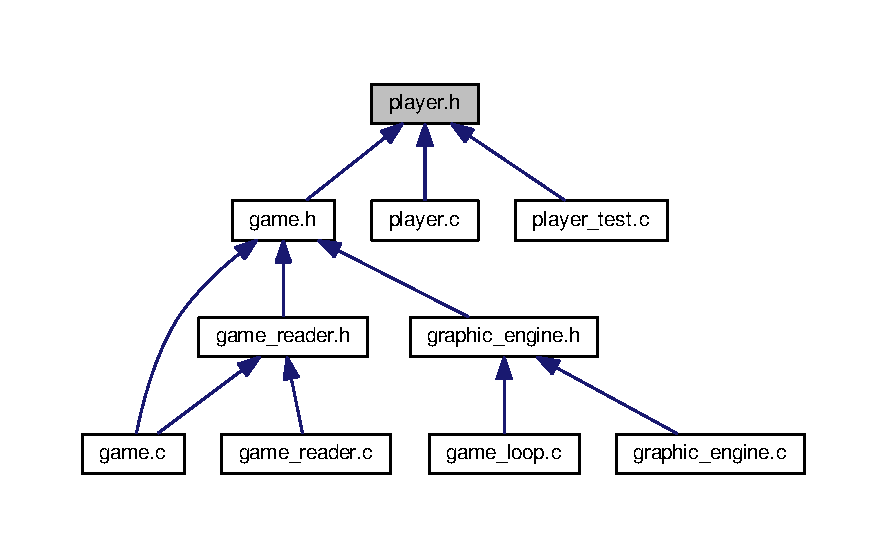
\includegraphics[width=350pt]{player_8h__dep__incl}
\end{center}
\end{figure}
\subsection*{Typedefs}
\begin{DoxyCompactItemize}
\item 
typedef struct \hyperlink{struct__Player}{\+\_\+\+Player} \hyperlink{player_8h_af30e2030635a69690f85e48bc6ef202f}{Player}
\end{DoxyCompactItemize}
\subsection*{Functions}
\begin{DoxyCompactItemize}
\item 
\hyperlink{player_8h_af30e2030635a69690f85e48bc6ef202f}{Player} $\ast$ \hyperlink{player_8h_a53dd0f330e7f77a2dd65594770abe65d}{player\+\_\+create} (char $\ast$, \hyperlink{types_8h_a845e604fb28f7e3d97549da3448149d3}{Id}, \hyperlink{types_8h_a845e604fb28f7e3d97549da3448149d3}{Id}, \hyperlink{types_8h_a845e604fb28f7e3d97549da3448149d3}{Id})
\item 
void \hyperlink{player_8h_aece75b2d89303f74dbe25c22138535b5}{player\+\_\+destroy} (\hyperlink{player_8h_af30e2030635a69690f85e48bc6ef202f}{Player} $\ast$)
\item 
\hyperlink{types_8h_a32c27cc471df37f4fc818d65de0a56c4}{S\+T\+A\+T\+US} \hyperlink{player_8h_a9f288e4b98a814b7f2ac4cfcfce1f4a5}{player\+\_\+set\+Name} (\hyperlink{player_8h_af30e2030635a69690f85e48bc6ef202f}{Player} $\ast$, char $\ast$)
\item 
\hyperlink{types_8h_a32c27cc471df37f4fc818d65de0a56c4}{S\+T\+A\+T\+US} \hyperlink{player_8h_a21c5c442b7fdbbe5f37555446bc06b22}{player\+\_\+set\+Loc\+Id} (\hyperlink{player_8h_af30e2030635a69690f85e48bc6ef202f}{Player} $\ast$, \hyperlink{types_8h_a845e604fb28f7e3d97549da3448149d3}{Id})
\item 
\hyperlink{types_8h_a32c27cc471df37f4fc818d65de0a56c4}{S\+T\+A\+T\+US} \hyperlink{player_8h_ac9b94a63b3af9250469560b9730abcd8}{player\+\_\+set\+Obj\+Id} (\hyperlink{player_8h_af30e2030635a69690f85e48bc6ef202f}{Player} $\ast$, \hyperlink{types_8h_a845e604fb28f7e3d97549da3448149d3}{Id})
\item 
\hyperlink{types_8h_a32c27cc471df37f4fc818d65de0a56c4}{S\+T\+A\+T\+US} \hyperlink{player_8h_a6c1a814774a540858c502e9c9fdb77ce}{player\+\_\+set\+Id} (\hyperlink{player_8h_af30e2030635a69690f85e48bc6ef202f}{Player} $\ast$, \hyperlink{types_8h_a845e604fb28f7e3d97549da3448149d3}{Id})
\item 
char $\ast$ \hyperlink{player_8h_aef33f133ed04df2e21f963474a3b469c}{player\+\_\+get\+Name} (\hyperlink{player_8h_af30e2030635a69690f85e48bc6ef202f}{Player} $\ast$)
\item 
\hyperlink{types_8h_a845e604fb28f7e3d97549da3448149d3}{Id} \hyperlink{player_8h_ae50e58151ba118762d98a3c9abb69ef1}{player\+\_\+get\+Loc\+Id} (\hyperlink{player_8h_af30e2030635a69690f85e48bc6ef202f}{Player} $\ast$)
\item 
\hyperlink{types_8h_a845e604fb28f7e3d97549da3448149d3}{Id} \hyperlink{player_8h_ad8ce15d22b7131c7c4fefe885c73fdbf}{player\+\_\+get\+Obj\+Id} (\hyperlink{player_8h_af30e2030635a69690f85e48bc6ef202f}{Player} $\ast$, int)
\item 
\hyperlink{types_8h_a845e604fb28f7e3d97549da3448149d3}{Id} \hyperlink{player_8h_a8bad69a1ee2f644a48ad2255711971d1}{player\+\_\+get\+Id} (\hyperlink{player_8h_af30e2030635a69690f85e48bc6ef202f}{Player} $\ast$)
\item 
\hyperlink{types_8h_a32c27cc471df37f4fc818d65de0a56c4}{S\+T\+A\+T\+US} \hyperlink{player_8h_afeaa065406f43d911349ee9f55903488}{player\+\_\+remove\+Obj\+Id} (\hyperlink{player_8h_af30e2030635a69690f85e48bc6ef202f}{Player} $\ast$, \hyperlink{types_8h_a845e604fb28f7e3d97549da3448149d3}{Id})
\end{DoxyCompactItemize}


\subsection{Detailed Description}
Functions for the creation of players. 

\begin{DoxyAuthor}{Author}
Guillermo Ríos 
\end{DoxyAuthor}
\begin{DoxyCopyright}{Copyright}
G\+NU Public License 
\end{DoxyCopyright}


\subsection{Typedef Documentation}
\index{player.\+h@{player.\+h}!Player@{Player}}
\index{Player@{Player}!player.\+h@{player.\+h}}
\subsubsection[{\texorpdfstring{Player}{Player}}]{\setlength{\rightskip}{0pt plus 5cm}typedef struct {\bf \+\_\+\+Player} {\bf Player}}\hypertarget{player_8h_af30e2030635a69690f85e48bc6ef202f}{}\label{player_8h_af30e2030635a69690f85e48bc6ef202f}


\subsection{Function Documentation}
\index{player.\+h@{player.\+h}!player\+\_\+create@{player\+\_\+create}}
\index{player\+\_\+create@{player\+\_\+create}!player.\+h@{player.\+h}}
\subsubsection[{\texorpdfstring{player\+\_\+create(char $\ast$, Id, Id, Id)}{player_create(char *, Id, Id, Id)}}]{\setlength{\rightskip}{0pt plus 5cm}{\bf Player}$\ast$ player\+\_\+create (
\begin{DoxyParamCaption}
\item[{char $\ast$}]{, }
\item[{{\bf Id}}]{, }
\item[{{\bf Id}}]{, }
\item[{{\bf Id}}]{}
\end{DoxyParamCaption}
)}\hypertarget{player_8h_a53dd0f330e7f77a2dd65594770abe65d}{}\label{player_8h_a53dd0f330e7f77a2dd65594770abe65d}
Returns null if no name is given to the player Returns pointer to the newly created player if ok\index{player.\+h@{player.\+h}!player\+\_\+destroy@{player\+\_\+destroy}}
\index{player\+\_\+destroy@{player\+\_\+destroy}!player.\+h@{player.\+h}}
\subsubsection[{\texorpdfstring{player\+\_\+destroy(\+Player $\ast$)}{player_destroy(Player *)}}]{\setlength{\rightskip}{0pt plus 5cm}void player\+\_\+destroy (
\begin{DoxyParamCaption}
\item[{{\bf Player} $\ast$}]{}
\end{DoxyParamCaption}
)}\hypertarget{player_8h_aece75b2d89303f74dbe25c22138535b5}{}\label{player_8h_aece75b2d89303f74dbe25c22138535b5}
\index{player.\+h@{player.\+h}!player\+\_\+get\+Id@{player\+\_\+get\+Id}}
\index{player\+\_\+get\+Id@{player\+\_\+get\+Id}!player.\+h@{player.\+h}}
\subsubsection[{\texorpdfstring{player\+\_\+get\+Id(\+Player $\ast$)}{player_getId(Player *)}}]{\setlength{\rightskip}{0pt plus 5cm}{\bf Id} player\+\_\+get\+Id (
\begin{DoxyParamCaption}
\item[{{\bf Player} $\ast$}]{}
\end{DoxyParamCaption}
)}\hypertarget{player_8h_a8bad69a1ee2f644a48ad2255711971d1}{}\label{player_8h_a8bad69a1ee2f644a48ad2255711971d1}
\index{player.\+h@{player.\+h}!player\+\_\+get\+Loc\+Id@{player\+\_\+get\+Loc\+Id}}
\index{player\+\_\+get\+Loc\+Id@{player\+\_\+get\+Loc\+Id}!player.\+h@{player.\+h}}
\subsubsection[{\texorpdfstring{player\+\_\+get\+Loc\+Id(\+Player $\ast$)}{player_getLocId(Player *)}}]{\setlength{\rightskip}{0pt plus 5cm}{\bf Id} player\+\_\+get\+Loc\+Id (
\begin{DoxyParamCaption}
\item[{{\bf Player} $\ast$}]{}
\end{DoxyParamCaption}
)}\hypertarget{player_8h_ae50e58151ba118762d98a3c9abb69ef1}{}\label{player_8h_ae50e58151ba118762d98a3c9abb69ef1}
\index{player.\+h@{player.\+h}!player\+\_\+get\+Name@{player\+\_\+get\+Name}}
\index{player\+\_\+get\+Name@{player\+\_\+get\+Name}!player.\+h@{player.\+h}}
\subsubsection[{\texorpdfstring{player\+\_\+get\+Name(\+Player $\ast$)}{player_getName(Player *)}}]{\setlength{\rightskip}{0pt plus 5cm}char$\ast$ player\+\_\+get\+Name (
\begin{DoxyParamCaption}
\item[{{\bf Player} $\ast$}]{}
\end{DoxyParamCaption}
)}\hypertarget{player_8h_aef33f133ed04df2e21f963474a3b469c}{}\label{player_8h_aef33f133ed04df2e21f963474a3b469c}
\index{player.\+h@{player.\+h}!player\+\_\+get\+Obj\+Id@{player\+\_\+get\+Obj\+Id}}
\index{player\+\_\+get\+Obj\+Id@{player\+\_\+get\+Obj\+Id}!player.\+h@{player.\+h}}
\subsubsection[{\texorpdfstring{player\+\_\+get\+Obj\+Id(\+Player $\ast$, int)}{player_getObjId(Player *, int)}}]{\setlength{\rightskip}{0pt plus 5cm}{\bf Id} player\+\_\+get\+Obj\+Id (
\begin{DoxyParamCaption}
\item[{{\bf Player} $\ast$}]{, }
\item[{int}]{}
\end{DoxyParamCaption}
)}\hypertarget{player_8h_ad8ce15d22b7131c7c4fefe885c73fdbf}{}\label{player_8h_ad8ce15d22b7131c7c4fefe885c73fdbf}
\index{player.\+h@{player.\+h}!player\+\_\+remove\+Obj\+Id@{player\+\_\+remove\+Obj\+Id}}
\index{player\+\_\+remove\+Obj\+Id@{player\+\_\+remove\+Obj\+Id}!player.\+h@{player.\+h}}
\subsubsection[{\texorpdfstring{player\+\_\+remove\+Obj\+Id(\+Player $\ast$, Id)}{player_removeObjId(Player *, Id)}}]{\setlength{\rightskip}{0pt plus 5cm}{\bf S\+T\+A\+T\+US} player\+\_\+remove\+Obj\+Id (
\begin{DoxyParamCaption}
\item[{{\bf Player} $\ast$}]{, }
\item[{{\bf Id}}]{}
\end{DoxyParamCaption}
)}\hypertarget{player_8h_afeaa065406f43d911349ee9f55903488}{}\label{player_8h_afeaa065406f43d911349ee9f55903488}
\index{player.\+h@{player.\+h}!player\+\_\+set\+Id@{player\+\_\+set\+Id}}
\index{player\+\_\+set\+Id@{player\+\_\+set\+Id}!player.\+h@{player.\+h}}
\subsubsection[{\texorpdfstring{player\+\_\+set\+Id(\+Player $\ast$, Id)}{player_setId(Player *, Id)}}]{\setlength{\rightskip}{0pt plus 5cm}{\bf S\+T\+A\+T\+US} player\+\_\+set\+Id (
\begin{DoxyParamCaption}
\item[{{\bf Player} $\ast$}]{, }
\item[{{\bf Id}}]{}
\end{DoxyParamCaption}
)}\hypertarget{player_8h_a6c1a814774a540858c502e9c9fdb77ce}{}\label{player_8h_a6c1a814774a540858c502e9c9fdb77ce}
\index{player.\+h@{player.\+h}!player\+\_\+set\+Loc\+Id@{player\+\_\+set\+Loc\+Id}}
\index{player\+\_\+set\+Loc\+Id@{player\+\_\+set\+Loc\+Id}!player.\+h@{player.\+h}}
\subsubsection[{\texorpdfstring{player\+\_\+set\+Loc\+Id(\+Player $\ast$, Id)}{player_setLocId(Player *, Id)}}]{\setlength{\rightskip}{0pt plus 5cm}{\bf S\+T\+A\+T\+US} player\+\_\+set\+Loc\+Id (
\begin{DoxyParamCaption}
\item[{{\bf Player} $\ast$}]{, }
\item[{{\bf Id}}]{}
\end{DoxyParamCaption}
)}\hypertarget{player_8h_a21c5c442b7fdbbe5f37555446bc06b22}{}\label{player_8h_a21c5c442b7fdbbe5f37555446bc06b22}
\index{player.\+h@{player.\+h}!player\+\_\+set\+Name@{player\+\_\+set\+Name}}
\index{player\+\_\+set\+Name@{player\+\_\+set\+Name}!player.\+h@{player.\+h}}
\subsubsection[{\texorpdfstring{player\+\_\+set\+Name(\+Player $\ast$, char $\ast$)}{player_setName(Player *, char *)}}]{\setlength{\rightskip}{0pt plus 5cm}{\bf S\+T\+A\+T\+US} player\+\_\+set\+Name (
\begin{DoxyParamCaption}
\item[{{\bf Player} $\ast$}]{, }
\item[{char $\ast$}]{}
\end{DoxyParamCaption}
)}\hypertarget{player_8h_a9f288e4b98a814b7f2ac4cfcfce1f4a5}{}\label{player_8h_a9f288e4b98a814b7f2ac4cfcfce1f4a5}
\index{player.\+h@{player.\+h}!player\+\_\+set\+Obj\+Id@{player\+\_\+set\+Obj\+Id}}
\index{player\+\_\+set\+Obj\+Id@{player\+\_\+set\+Obj\+Id}!player.\+h@{player.\+h}}
\subsubsection[{\texorpdfstring{player\+\_\+set\+Obj\+Id(\+Player $\ast$, Id)}{player_setObjId(Player *, Id)}}]{\setlength{\rightskip}{0pt plus 5cm}{\bf S\+T\+A\+T\+US} player\+\_\+set\+Obj\+Id (
\begin{DoxyParamCaption}
\item[{{\bf Player} $\ast$}]{, }
\item[{{\bf Id}}]{}
\end{DoxyParamCaption}
)}\hypertarget{player_8h_ac9b94a63b3af9250469560b9730abcd8}{}\label{player_8h_ac9b94a63b3af9250469560b9730abcd8}

\hypertarget{player__test_8c}{\section{player\+\_\+test.\+c File Reference}
\label{player__test_8c}\index{player\+\_\+test.\+c@{player\+\_\+test.\+c}}
}
{\ttfamily \#include $<$stdio.\+h$>$}\\*
{\ttfamily \#include $<$stdlib.\+h$>$}\\*
{\ttfamily \#include $<$string.\+h$>$}\\*
{\ttfamily \#include \char`\"{}../include/player.\+h\char`\"{}}\\*
{\ttfamily \#include \char`\"{}../include/player\+\_\+test.\+h\char`\"{}}\\*
{\ttfamily \#include \char`\"{}../include/test.\+h\char`\"{}}\\*
Include dependency graph for player\+\_\+test.\+c\+:\nopagebreak
\begin{figure}[H]
\begin{center}
\leavevmode
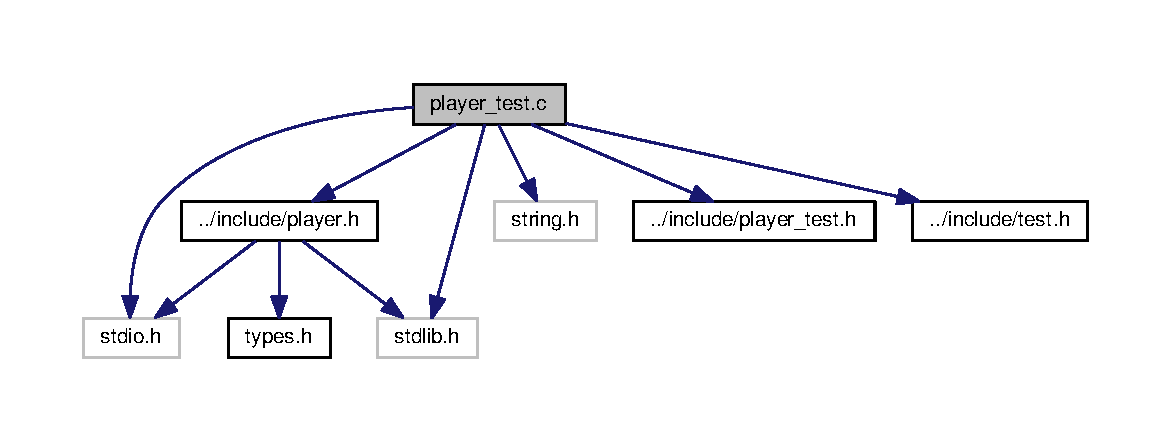
\includegraphics[width=350pt]{player__test_8c__incl}
\end{center}
\end{figure}
\subsection*{Macros}
\begin{DoxyCompactItemize}
\item 
\#define \hyperlink{player__test_8c_a2a77d2f2c5b698c69c19e1f8782bf709}{M\+A\+X\+\_\+\+T\+E\+S\+T\+S}~16
\end{DoxyCompactItemize}
\subsection*{Functions}
\begin{DoxyCompactItemize}
\item 
int \hyperlink{player__test_8c_a3c04138a5bfe5d72780bb7e82a18e627}{main} (int argc, char $\ast$$\ast$argv)
\begin{DoxyCompactList}\small\item\em Funcion principal de pruebas para el modulo Space. \end{DoxyCompactList}\item 
void \hyperlink{player__test_8c_ab29768452373e16bb6aaa1f7998f62fb}{test1\+\_\+player\+\_\+create} ()
\item 
void \hyperlink{player__test_8c_a9d87c09e6af910d695265e3fd77ae3a2}{test1\+\_\+player\+\_\+set\+\_\+name} ()
\item 
void \hyperlink{player__test_8c_a6e7ce8ff791f4bf63749df647a44263f}{test2\+\_\+player\+\_\+set\+\_\+name} ()
\item 
void \hyperlink{player__test_8c_acdc4553cbf87881a05d4b33604a51913}{test1\+\_\+player\+\_\+set\+\_\+\+Loc\+Id} ()
\item 
void \hyperlink{player__test_8c_ac801de2cba19dfc3912d66d64461243c}{test2\+\_\+player\+\_\+set\+\_\+\+Loc\+Id} ()
\item 
void \hyperlink{player__test_8c_a3d5d1f9f05f2909e999eda4f3e2d2a66}{test1\+\_\+player\+\_\+set\+\_\+\+Obj\+Id} ()
\item 
void \hyperlink{player__test_8c_a600034aa20583bc42a30327c0bb1ddd4}{test2\+\_\+player\+\_\+set\+\_\+\+Obj\+Id} ()
\item 
void \hyperlink{player__test_8c_a64fa15a235953bea694236b9d7841cbc}{test1\+\_\+player\+\_\+set\+\_\+id} ()
\item 
void \hyperlink{player__test_8c_a3695e0896bc3d770290e6a691fa212f7}{test2\+\_\+player\+\_\+set\+\_\+id} ()
\item 
void \hyperlink{player__test_8c_a94068667d8faa66a4ad293dd2c60f2ef}{test1\+\_\+player\+\_\+get\+\_\+name} ()
\item 
void \hyperlink{player__test_8c_a21c23574d847f00133599005f1e4262f}{test1\+\_\+player\+\_\+get\+\_\+\+Loc\+Id} ()
\item 
void \hyperlink{player__test_8c_a8c7e112bade03a60dd8b5cfc235f1a0c}{test1\+\_\+player\+\_\+get\+\_\+\+Obj\+Id} ()
\item 
void \hyperlink{player__test_8c_a790a75dc179c00c60c784d3e34c0e5aa}{test1\+\_\+player\+\_\+get\+\_\+id} ()
\item 
void \hyperlink{player__test_8c_a880117fe48daf4386e5813efd19fa315}{test1\+\_\+player\+\_\+remove\+\_\+object\+\_\+id} ()
\item 
void \hyperlink{player__test_8c_a701c881623ca996aa99adadc6cdc0e98}{test2\+\_\+player\+\_\+remove\+\_\+object\+\_\+id} ()
\end{DoxyCompactItemize}


\subsection{Macro Definition Documentation}
\hypertarget{player__test_8c_a2a77d2f2c5b698c69c19e1f8782bf709}{\index{player\+\_\+test.\+c@{player\+\_\+test.\+c}!M\+A\+X\+\_\+\+T\+E\+S\+T\+S@{M\+A\+X\+\_\+\+T\+E\+S\+T\+S}}
\index{M\+A\+X\+\_\+\+T\+E\+S\+T\+S@{M\+A\+X\+\_\+\+T\+E\+S\+T\+S}!player\+\_\+test.\+c@{player\+\_\+test.\+c}}
\subsubsection[{M\+A\+X\+\_\+\+T\+E\+S\+T\+S}]{\setlength{\rightskip}{0pt plus 5cm}\#define M\+A\+X\+\_\+\+T\+E\+S\+T\+S~16}}\label{player__test_8c_a2a77d2f2c5b698c69c19e1f8782bf709}


\subsection{Function Documentation}
\hypertarget{player__test_8c_a3c04138a5bfe5d72780bb7e82a18e627}{\index{player\+\_\+test.\+c@{player\+\_\+test.\+c}!main@{main}}
\index{main@{main}!player\+\_\+test.\+c@{player\+\_\+test.\+c}}
\subsubsection[{main}]{\setlength{\rightskip}{0pt plus 5cm}int main (
\begin{DoxyParamCaption}
\item[{int}]{argc, }
\item[{char $\ast$$\ast$}]{argv}
\end{DoxyParamCaption}
)}}\label{player__test_8c_a3c04138a5bfe5d72780bb7e82a18e627}


Funcion principal de pruebas para el modulo Space. 

Dos modos de ejecucion\+: 1.-\/\+Si se ejecuta sin parametros se ejecutan todas las pruebas 2.-\/\+Si se ejecuta con un numero entre 1 y el numero de pruebas solo ejecuta la prueba indicada \hypertarget{player__test_8c_ab29768452373e16bb6aaa1f7998f62fb}{\index{player\+\_\+test.\+c@{player\+\_\+test.\+c}!test1\+\_\+player\+\_\+create@{test1\+\_\+player\+\_\+create}}
\index{test1\+\_\+player\+\_\+create@{test1\+\_\+player\+\_\+create}!player\+\_\+test.\+c@{player\+\_\+test.\+c}}
\subsubsection[{test1\+\_\+player\+\_\+create}]{\setlength{\rightskip}{0pt plus 5cm}void test1\+\_\+player\+\_\+create (
\begin{DoxyParamCaption}
{}
\end{DoxyParamCaption}
)}}\label{player__test_8c_ab29768452373e16bb6aaa1f7998f62fb}
\hypertarget{player__test_8c_a790a75dc179c00c60c784d3e34c0e5aa}{\index{player\+\_\+test.\+c@{player\+\_\+test.\+c}!test1\+\_\+player\+\_\+get\+\_\+id@{test1\+\_\+player\+\_\+get\+\_\+id}}
\index{test1\+\_\+player\+\_\+get\+\_\+id@{test1\+\_\+player\+\_\+get\+\_\+id}!player\+\_\+test.\+c@{player\+\_\+test.\+c}}
\subsubsection[{test1\+\_\+player\+\_\+get\+\_\+id}]{\setlength{\rightskip}{0pt plus 5cm}void test1\+\_\+player\+\_\+get\+\_\+id (
\begin{DoxyParamCaption}
{}
\end{DoxyParamCaption}
)}}\label{player__test_8c_a790a75dc179c00c60c784d3e34c0e5aa}
\hypertarget{player__test_8c_a21c23574d847f00133599005f1e4262f}{\index{player\+\_\+test.\+c@{player\+\_\+test.\+c}!test1\+\_\+player\+\_\+get\+\_\+\+Loc\+Id@{test1\+\_\+player\+\_\+get\+\_\+\+Loc\+Id}}
\index{test1\+\_\+player\+\_\+get\+\_\+\+Loc\+Id@{test1\+\_\+player\+\_\+get\+\_\+\+Loc\+Id}!player\+\_\+test.\+c@{player\+\_\+test.\+c}}
\subsubsection[{test1\+\_\+player\+\_\+get\+\_\+\+Loc\+Id}]{\setlength{\rightskip}{0pt plus 5cm}void test1\+\_\+player\+\_\+get\+\_\+\+Loc\+Id (
\begin{DoxyParamCaption}
{}
\end{DoxyParamCaption}
)}}\label{player__test_8c_a21c23574d847f00133599005f1e4262f}
\hypertarget{player__test_8c_a94068667d8faa66a4ad293dd2c60f2ef}{\index{player\+\_\+test.\+c@{player\+\_\+test.\+c}!test1\+\_\+player\+\_\+get\+\_\+name@{test1\+\_\+player\+\_\+get\+\_\+name}}
\index{test1\+\_\+player\+\_\+get\+\_\+name@{test1\+\_\+player\+\_\+get\+\_\+name}!player\+\_\+test.\+c@{player\+\_\+test.\+c}}
\subsubsection[{test1\+\_\+player\+\_\+get\+\_\+name}]{\setlength{\rightskip}{0pt plus 5cm}void test1\+\_\+player\+\_\+get\+\_\+name (
\begin{DoxyParamCaption}
{}
\end{DoxyParamCaption}
)}}\label{player__test_8c_a94068667d8faa66a4ad293dd2c60f2ef}
\hypertarget{player__test_8c_a8c7e112bade03a60dd8b5cfc235f1a0c}{\index{player\+\_\+test.\+c@{player\+\_\+test.\+c}!test1\+\_\+player\+\_\+get\+\_\+\+Obj\+Id@{test1\+\_\+player\+\_\+get\+\_\+\+Obj\+Id}}
\index{test1\+\_\+player\+\_\+get\+\_\+\+Obj\+Id@{test1\+\_\+player\+\_\+get\+\_\+\+Obj\+Id}!player\+\_\+test.\+c@{player\+\_\+test.\+c}}
\subsubsection[{test1\+\_\+player\+\_\+get\+\_\+\+Obj\+Id}]{\setlength{\rightskip}{0pt plus 5cm}void test1\+\_\+player\+\_\+get\+\_\+\+Obj\+Id (
\begin{DoxyParamCaption}
{}
\end{DoxyParamCaption}
)}}\label{player__test_8c_a8c7e112bade03a60dd8b5cfc235f1a0c}
\hypertarget{player__test_8c_a880117fe48daf4386e5813efd19fa315}{\index{player\+\_\+test.\+c@{player\+\_\+test.\+c}!test1\+\_\+player\+\_\+remove\+\_\+object\+\_\+id@{test1\+\_\+player\+\_\+remove\+\_\+object\+\_\+id}}
\index{test1\+\_\+player\+\_\+remove\+\_\+object\+\_\+id@{test1\+\_\+player\+\_\+remove\+\_\+object\+\_\+id}!player\+\_\+test.\+c@{player\+\_\+test.\+c}}
\subsubsection[{test1\+\_\+player\+\_\+remove\+\_\+object\+\_\+id}]{\setlength{\rightskip}{0pt plus 5cm}void test1\+\_\+player\+\_\+remove\+\_\+object\+\_\+id (
\begin{DoxyParamCaption}
{}
\end{DoxyParamCaption}
)}}\label{player__test_8c_a880117fe48daf4386e5813efd19fa315}
\hypertarget{player__test_8c_a64fa15a235953bea694236b9d7841cbc}{\index{player\+\_\+test.\+c@{player\+\_\+test.\+c}!test1\+\_\+player\+\_\+set\+\_\+id@{test1\+\_\+player\+\_\+set\+\_\+id}}
\index{test1\+\_\+player\+\_\+set\+\_\+id@{test1\+\_\+player\+\_\+set\+\_\+id}!player\+\_\+test.\+c@{player\+\_\+test.\+c}}
\subsubsection[{test1\+\_\+player\+\_\+set\+\_\+id}]{\setlength{\rightskip}{0pt plus 5cm}void test1\+\_\+player\+\_\+set\+\_\+id (
\begin{DoxyParamCaption}
{}
\end{DoxyParamCaption}
)}}\label{player__test_8c_a64fa15a235953bea694236b9d7841cbc}
\hypertarget{player__test_8c_acdc4553cbf87881a05d4b33604a51913}{\index{player\+\_\+test.\+c@{player\+\_\+test.\+c}!test1\+\_\+player\+\_\+set\+\_\+\+Loc\+Id@{test1\+\_\+player\+\_\+set\+\_\+\+Loc\+Id}}
\index{test1\+\_\+player\+\_\+set\+\_\+\+Loc\+Id@{test1\+\_\+player\+\_\+set\+\_\+\+Loc\+Id}!player\+\_\+test.\+c@{player\+\_\+test.\+c}}
\subsubsection[{test1\+\_\+player\+\_\+set\+\_\+\+Loc\+Id}]{\setlength{\rightskip}{0pt plus 5cm}void test1\+\_\+player\+\_\+set\+\_\+\+Loc\+Id (
\begin{DoxyParamCaption}
{}
\end{DoxyParamCaption}
)}}\label{player__test_8c_acdc4553cbf87881a05d4b33604a51913}
\hypertarget{player__test_8c_a9d87c09e6af910d695265e3fd77ae3a2}{\index{player\+\_\+test.\+c@{player\+\_\+test.\+c}!test1\+\_\+player\+\_\+set\+\_\+name@{test1\+\_\+player\+\_\+set\+\_\+name}}
\index{test1\+\_\+player\+\_\+set\+\_\+name@{test1\+\_\+player\+\_\+set\+\_\+name}!player\+\_\+test.\+c@{player\+\_\+test.\+c}}
\subsubsection[{test1\+\_\+player\+\_\+set\+\_\+name}]{\setlength{\rightskip}{0pt plus 5cm}void test1\+\_\+player\+\_\+set\+\_\+name (
\begin{DoxyParamCaption}
{}
\end{DoxyParamCaption}
)}}\label{player__test_8c_a9d87c09e6af910d695265e3fd77ae3a2}
\hypertarget{player__test_8c_a3d5d1f9f05f2909e999eda4f3e2d2a66}{\index{player\+\_\+test.\+c@{player\+\_\+test.\+c}!test1\+\_\+player\+\_\+set\+\_\+\+Obj\+Id@{test1\+\_\+player\+\_\+set\+\_\+\+Obj\+Id}}
\index{test1\+\_\+player\+\_\+set\+\_\+\+Obj\+Id@{test1\+\_\+player\+\_\+set\+\_\+\+Obj\+Id}!player\+\_\+test.\+c@{player\+\_\+test.\+c}}
\subsubsection[{test1\+\_\+player\+\_\+set\+\_\+\+Obj\+Id}]{\setlength{\rightskip}{0pt plus 5cm}void test1\+\_\+player\+\_\+set\+\_\+\+Obj\+Id (
\begin{DoxyParamCaption}
{}
\end{DoxyParamCaption}
)}}\label{player__test_8c_a3d5d1f9f05f2909e999eda4f3e2d2a66}
\hypertarget{player__test_8c_a701c881623ca996aa99adadc6cdc0e98}{\index{player\+\_\+test.\+c@{player\+\_\+test.\+c}!test2\+\_\+player\+\_\+remove\+\_\+object\+\_\+id@{test2\+\_\+player\+\_\+remove\+\_\+object\+\_\+id}}
\index{test2\+\_\+player\+\_\+remove\+\_\+object\+\_\+id@{test2\+\_\+player\+\_\+remove\+\_\+object\+\_\+id}!player\+\_\+test.\+c@{player\+\_\+test.\+c}}
\subsubsection[{test2\+\_\+player\+\_\+remove\+\_\+object\+\_\+id}]{\setlength{\rightskip}{0pt plus 5cm}void test2\+\_\+player\+\_\+remove\+\_\+object\+\_\+id (
\begin{DoxyParamCaption}
{}
\end{DoxyParamCaption}
)}}\label{player__test_8c_a701c881623ca996aa99adadc6cdc0e98}
\hypertarget{player__test_8c_a3695e0896bc3d770290e6a691fa212f7}{\index{player\+\_\+test.\+c@{player\+\_\+test.\+c}!test2\+\_\+player\+\_\+set\+\_\+id@{test2\+\_\+player\+\_\+set\+\_\+id}}
\index{test2\+\_\+player\+\_\+set\+\_\+id@{test2\+\_\+player\+\_\+set\+\_\+id}!player\+\_\+test.\+c@{player\+\_\+test.\+c}}
\subsubsection[{test2\+\_\+player\+\_\+set\+\_\+id}]{\setlength{\rightskip}{0pt plus 5cm}void test2\+\_\+player\+\_\+set\+\_\+id (
\begin{DoxyParamCaption}
{}
\end{DoxyParamCaption}
)}}\label{player__test_8c_a3695e0896bc3d770290e6a691fa212f7}
\hypertarget{player__test_8c_ac801de2cba19dfc3912d66d64461243c}{\index{player\+\_\+test.\+c@{player\+\_\+test.\+c}!test2\+\_\+player\+\_\+set\+\_\+\+Loc\+Id@{test2\+\_\+player\+\_\+set\+\_\+\+Loc\+Id}}
\index{test2\+\_\+player\+\_\+set\+\_\+\+Loc\+Id@{test2\+\_\+player\+\_\+set\+\_\+\+Loc\+Id}!player\+\_\+test.\+c@{player\+\_\+test.\+c}}
\subsubsection[{test2\+\_\+player\+\_\+set\+\_\+\+Loc\+Id}]{\setlength{\rightskip}{0pt plus 5cm}void test2\+\_\+player\+\_\+set\+\_\+\+Loc\+Id (
\begin{DoxyParamCaption}
{}
\end{DoxyParamCaption}
)}}\label{player__test_8c_ac801de2cba19dfc3912d66d64461243c}
\hypertarget{player__test_8c_a6e7ce8ff791f4bf63749df647a44263f}{\index{player\+\_\+test.\+c@{player\+\_\+test.\+c}!test2\+\_\+player\+\_\+set\+\_\+name@{test2\+\_\+player\+\_\+set\+\_\+name}}
\index{test2\+\_\+player\+\_\+set\+\_\+name@{test2\+\_\+player\+\_\+set\+\_\+name}!player\+\_\+test.\+c@{player\+\_\+test.\+c}}
\subsubsection[{test2\+\_\+player\+\_\+set\+\_\+name}]{\setlength{\rightskip}{0pt plus 5cm}void test2\+\_\+player\+\_\+set\+\_\+name (
\begin{DoxyParamCaption}
{}
\end{DoxyParamCaption}
)}}\label{player__test_8c_a6e7ce8ff791f4bf63749df647a44263f}
\hypertarget{player__test_8c_a600034aa20583bc42a30327c0bb1ddd4}{\index{player\+\_\+test.\+c@{player\+\_\+test.\+c}!test2\+\_\+player\+\_\+set\+\_\+\+Obj\+Id@{test2\+\_\+player\+\_\+set\+\_\+\+Obj\+Id}}
\index{test2\+\_\+player\+\_\+set\+\_\+\+Obj\+Id@{test2\+\_\+player\+\_\+set\+\_\+\+Obj\+Id}!player\+\_\+test.\+c@{player\+\_\+test.\+c}}
\subsubsection[{test2\+\_\+player\+\_\+set\+\_\+\+Obj\+Id}]{\setlength{\rightskip}{0pt plus 5cm}void test2\+\_\+player\+\_\+set\+\_\+\+Obj\+Id (
\begin{DoxyParamCaption}
{}
\end{DoxyParamCaption}
)}}\label{player__test_8c_a600034aa20583bc42a30327c0bb1ddd4}

\hypertarget{player__test_8h}{}\section{player\+\_\+test.\+h File Reference}
\label{player__test_8h}\index{player\+\_\+test.\+h@{player\+\_\+test.\+h}}


It declares the tests for the player module.  


This graph shows which files directly or indirectly include this file\+:\nopagebreak
\begin{figure}[H]
\begin{center}
\leavevmode
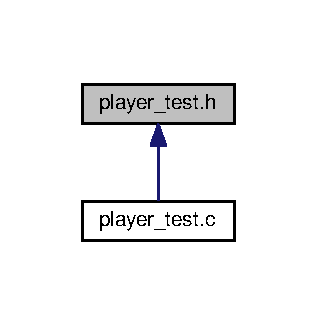
\includegraphics[width=152pt]{player__test_8h__dep__incl}
\end{center}
\end{figure}
\subsection*{Functions}
\begin{DoxyCompactItemize}
\item 
void \hyperlink{player__test_8h_ab29768452373e16bb6aaa1f7998f62fb}{test1\+\_\+player\+\_\+create} ()
\item 
void \hyperlink{player__test_8h_a9d87c09e6af910d695265e3fd77ae3a2}{test1\+\_\+player\+\_\+set\+\_\+name} ()
\item 
void \hyperlink{player__test_8h_a6e7ce8ff791f4bf63749df647a44263f}{test2\+\_\+player\+\_\+set\+\_\+name} ()
\item 
void \hyperlink{player__test_8h_acdc4553cbf87881a05d4b33604a51913}{test1\+\_\+player\+\_\+set\+\_\+\+Loc\+Id} ()
\item 
void \hyperlink{player__test_8h_ac801de2cba19dfc3912d66d64461243c}{test2\+\_\+player\+\_\+set\+\_\+\+Loc\+Id} ()
\item 
void \hyperlink{player__test_8h_a3d5d1f9f05f2909e999eda4f3e2d2a66}{test1\+\_\+player\+\_\+set\+\_\+\+Obj\+Id} ()
\item 
void \hyperlink{player__test_8h_a600034aa20583bc42a30327c0bb1ddd4}{test2\+\_\+player\+\_\+set\+\_\+\+Obj\+Id} ()
\item 
void \hyperlink{player__test_8h_a64fa15a235953bea694236b9d7841cbc}{test1\+\_\+player\+\_\+set\+\_\+id} ()
\item 
void \hyperlink{player__test_8h_a3695e0896bc3d770290e6a691fa212f7}{test2\+\_\+player\+\_\+set\+\_\+id} ()
\item 
void \hyperlink{player__test_8h_a94068667d8faa66a4ad293dd2c60f2ef}{test1\+\_\+player\+\_\+get\+\_\+name} ()
\item 
void \hyperlink{player__test_8h_a21c23574d847f00133599005f1e4262f}{test1\+\_\+player\+\_\+get\+\_\+\+Loc\+Id} ()
\item 
void \hyperlink{player__test_8h_a8c7e112bade03a60dd8b5cfc235f1a0c}{test1\+\_\+player\+\_\+get\+\_\+\+Obj\+Id} ()
\item 
void \hyperlink{player__test_8h_a790a75dc179c00c60c784d3e34c0e5aa}{test1\+\_\+player\+\_\+get\+\_\+id} ()
\item 
void \hyperlink{player__test_8h_a880117fe48daf4386e5813efd19fa315}{test1\+\_\+player\+\_\+remove\+\_\+object\+\_\+id} ()
\item 
void \hyperlink{player__test_8h_a701c881623ca996aa99adadc6cdc0e98}{test2\+\_\+player\+\_\+remove\+\_\+object\+\_\+id} ()
\end{DoxyCompactItemize}


\subsection{Detailed Description}
It declares the tests for the player module. 

\begin{DoxyAuthor}{Author}
Pablo Sánchez Redondo 
\end{DoxyAuthor}
\begin{DoxyCopyright}{Copyright}
G\+NU Public License 
\end{DoxyCopyright}


\subsection{Function Documentation}
\index{player\+\_\+test.\+h@{player\+\_\+test.\+h}!test1\+\_\+player\+\_\+create@{test1\+\_\+player\+\_\+create}}
\index{test1\+\_\+player\+\_\+create@{test1\+\_\+player\+\_\+create}!player\+\_\+test.\+h@{player\+\_\+test.\+h}}
\subsubsection[{\texorpdfstring{test1\+\_\+player\+\_\+create()}{test1_player_create()}}]{\setlength{\rightskip}{0pt plus 5cm}void test1\+\_\+player\+\_\+create (
\begin{DoxyParamCaption}
{}
\end{DoxyParamCaption}
)}\hypertarget{player__test_8h_ab29768452373e16bb6aaa1f7998f62fb}{}\label{player__test_8h_ab29768452373e16bb6aaa1f7998f62fb}
\index{player\+\_\+test.\+h@{player\+\_\+test.\+h}!test1\+\_\+player\+\_\+get\+\_\+id@{test1\+\_\+player\+\_\+get\+\_\+id}}
\index{test1\+\_\+player\+\_\+get\+\_\+id@{test1\+\_\+player\+\_\+get\+\_\+id}!player\+\_\+test.\+h@{player\+\_\+test.\+h}}
\subsubsection[{\texorpdfstring{test1\+\_\+player\+\_\+get\+\_\+id()}{test1_player_get_id()}}]{\setlength{\rightskip}{0pt plus 5cm}void test1\+\_\+player\+\_\+get\+\_\+id (
\begin{DoxyParamCaption}
{}
\end{DoxyParamCaption}
)}\hypertarget{player__test_8h_a790a75dc179c00c60c784d3e34c0e5aa}{}\label{player__test_8h_a790a75dc179c00c60c784d3e34c0e5aa}
\index{player\+\_\+test.\+h@{player\+\_\+test.\+h}!test1\+\_\+player\+\_\+get\+\_\+\+Loc\+Id@{test1\+\_\+player\+\_\+get\+\_\+\+Loc\+Id}}
\index{test1\+\_\+player\+\_\+get\+\_\+\+Loc\+Id@{test1\+\_\+player\+\_\+get\+\_\+\+Loc\+Id}!player\+\_\+test.\+h@{player\+\_\+test.\+h}}
\subsubsection[{\texorpdfstring{test1\+\_\+player\+\_\+get\+\_\+\+Loc\+Id()}{test1_player_get_LocId()}}]{\setlength{\rightskip}{0pt plus 5cm}void test1\+\_\+player\+\_\+get\+\_\+\+Loc\+Id (
\begin{DoxyParamCaption}
{}
\end{DoxyParamCaption}
)}\hypertarget{player__test_8h_a21c23574d847f00133599005f1e4262f}{}\label{player__test_8h_a21c23574d847f00133599005f1e4262f}
\index{player\+\_\+test.\+h@{player\+\_\+test.\+h}!test1\+\_\+player\+\_\+get\+\_\+name@{test1\+\_\+player\+\_\+get\+\_\+name}}
\index{test1\+\_\+player\+\_\+get\+\_\+name@{test1\+\_\+player\+\_\+get\+\_\+name}!player\+\_\+test.\+h@{player\+\_\+test.\+h}}
\subsubsection[{\texorpdfstring{test1\+\_\+player\+\_\+get\+\_\+name()}{test1_player_get_name()}}]{\setlength{\rightskip}{0pt plus 5cm}void test1\+\_\+player\+\_\+get\+\_\+name (
\begin{DoxyParamCaption}
{}
\end{DoxyParamCaption}
)}\hypertarget{player__test_8h_a94068667d8faa66a4ad293dd2c60f2ef}{}\label{player__test_8h_a94068667d8faa66a4ad293dd2c60f2ef}
\index{player\+\_\+test.\+h@{player\+\_\+test.\+h}!test1\+\_\+player\+\_\+get\+\_\+\+Obj\+Id@{test1\+\_\+player\+\_\+get\+\_\+\+Obj\+Id}}
\index{test1\+\_\+player\+\_\+get\+\_\+\+Obj\+Id@{test1\+\_\+player\+\_\+get\+\_\+\+Obj\+Id}!player\+\_\+test.\+h@{player\+\_\+test.\+h}}
\subsubsection[{\texorpdfstring{test1\+\_\+player\+\_\+get\+\_\+\+Obj\+Id()}{test1_player_get_ObjId()}}]{\setlength{\rightskip}{0pt plus 5cm}void test1\+\_\+player\+\_\+get\+\_\+\+Obj\+Id (
\begin{DoxyParamCaption}
{}
\end{DoxyParamCaption}
)}\hypertarget{player__test_8h_a8c7e112bade03a60dd8b5cfc235f1a0c}{}\label{player__test_8h_a8c7e112bade03a60dd8b5cfc235f1a0c}
\index{player\+\_\+test.\+h@{player\+\_\+test.\+h}!test1\+\_\+player\+\_\+remove\+\_\+object\+\_\+id@{test1\+\_\+player\+\_\+remove\+\_\+object\+\_\+id}}
\index{test1\+\_\+player\+\_\+remove\+\_\+object\+\_\+id@{test1\+\_\+player\+\_\+remove\+\_\+object\+\_\+id}!player\+\_\+test.\+h@{player\+\_\+test.\+h}}
\subsubsection[{\texorpdfstring{test1\+\_\+player\+\_\+remove\+\_\+object\+\_\+id()}{test1_player_remove_object_id()}}]{\setlength{\rightskip}{0pt plus 5cm}void test1\+\_\+player\+\_\+remove\+\_\+object\+\_\+id (
\begin{DoxyParamCaption}
{}
\end{DoxyParamCaption}
)}\hypertarget{player__test_8h_a880117fe48daf4386e5813efd19fa315}{}\label{player__test_8h_a880117fe48daf4386e5813efd19fa315}
\index{player\+\_\+test.\+h@{player\+\_\+test.\+h}!test1\+\_\+player\+\_\+set\+\_\+id@{test1\+\_\+player\+\_\+set\+\_\+id}}
\index{test1\+\_\+player\+\_\+set\+\_\+id@{test1\+\_\+player\+\_\+set\+\_\+id}!player\+\_\+test.\+h@{player\+\_\+test.\+h}}
\subsubsection[{\texorpdfstring{test1\+\_\+player\+\_\+set\+\_\+id()}{test1_player_set_id()}}]{\setlength{\rightskip}{0pt plus 5cm}void test1\+\_\+player\+\_\+set\+\_\+id (
\begin{DoxyParamCaption}
{}
\end{DoxyParamCaption}
)}\hypertarget{player__test_8h_a64fa15a235953bea694236b9d7841cbc}{}\label{player__test_8h_a64fa15a235953bea694236b9d7841cbc}
\index{player\+\_\+test.\+h@{player\+\_\+test.\+h}!test1\+\_\+player\+\_\+set\+\_\+\+Loc\+Id@{test1\+\_\+player\+\_\+set\+\_\+\+Loc\+Id}}
\index{test1\+\_\+player\+\_\+set\+\_\+\+Loc\+Id@{test1\+\_\+player\+\_\+set\+\_\+\+Loc\+Id}!player\+\_\+test.\+h@{player\+\_\+test.\+h}}
\subsubsection[{\texorpdfstring{test1\+\_\+player\+\_\+set\+\_\+\+Loc\+Id()}{test1_player_set_LocId()}}]{\setlength{\rightskip}{0pt plus 5cm}void test1\+\_\+player\+\_\+set\+\_\+\+Loc\+Id (
\begin{DoxyParamCaption}
{}
\end{DoxyParamCaption}
)}\hypertarget{player__test_8h_acdc4553cbf87881a05d4b33604a51913}{}\label{player__test_8h_acdc4553cbf87881a05d4b33604a51913}
\index{player\+\_\+test.\+h@{player\+\_\+test.\+h}!test1\+\_\+player\+\_\+set\+\_\+name@{test1\+\_\+player\+\_\+set\+\_\+name}}
\index{test1\+\_\+player\+\_\+set\+\_\+name@{test1\+\_\+player\+\_\+set\+\_\+name}!player\+\_\+test.\+h@{player\+\_\+test.\+h}}
\subsubsection[{\texorpdfstring{test1\+\_\+player\+\_\+set\+\_\+name()}{test1_player_set_name()}}]{\setlength{\rightskip}{0pt plus 5cm}void test1\+\_\+player\+\_\+set\+\_\+name (
\begin{DoxyParamCaption}
{}
\end{DoxyParamCaption}
)}\hypertarget{player__test_8h_a9d87c09e6af910d695265e3fd77ae3a2}{}\label{player__test_8h_a9d87c09e6af910d695265e3fd77ae3a2}
\index{player\+\_\+test.\+h@{player\+\_\+test.\+h}!test1\+\_\+player\+\_\+set\+\_\+\+Obj\+Id@{test1\+\_\+player\+\_\+set\+\_\+\+Obj\+Id}}
\index{test1\+\_\+player\+\_\+set\+\_\+\+Obj\+Id@{test1\+\_\+player\+\_\+set\+\_\+\+Obj\+Id}!player\+\_\+test.\+h@{player\+\_\+test.\+h}}
\subsubsection[{\texorpdfstring{test1\+\_\+player\+\_\+set\+\_\+\+Obj\+Id()}{test1_player_set_ObjId()}}]{\setlength{\rightskip}{0pt plus 5cm}void test1\+\_\+player\+\_\+set\+\_\+\+Obj\+Id (
\begin{DoxyParamCaption}
{}
\end{DoxyParamCaption}
)}\hypertarget{player__test_8h_a3d5d1f9f05f2909e999eda4f3e2d2a66}{}\label{player__test_8h_a3d5d1f9f05f2909e999eda4f3e2d2a66}
\index{player\+\_\+test.\+h@{player\+\_\+test.\+h}!test2\+\_\+player\+\_\+remove\+\_\+object\+\_\+id@{test2\+\_\+player\+\_\+remove\+\_\+object\+\_\+id}}
\index{test2\+\_\+player\+\_\+remove\+\_\+object\+\_\+id@{test2\+\_\+player\+\_\+remove\+\_\+object\+\_\+id}!player\+\_\+test.\+h@{player\+\_\+test.\+h}}
\subsubsection[{\texorpdfstring{test2\+\_\+player\+\_\+remove\+\_\+object\+\_\+id()}{test2_player_remove_object_id()}}]{\setlength{\rightskip}{0pt plus 5cm}void test2\+\_\+player\+\_\+remove\+\_\+object\+\_\+id (
\begin{DoxyParamCaption}
{}
\end{DoxyParamCaption}
)}\hypertarget{player__test_8h_a701c881623ca996aa99adadc6cdc0e98}{}\label{player__test_8h_a701c881623ca996aa99adadc6cdc0e98}
\index{player\+\_\+test.\+h@{player\+\_\+test.\+h}!test2\+\_\+player\+\_\+set\+\_\+id@{test2\+\_\+player\+\_\+set\+\_\+id}}
\index{test2\+\_\+player\+\_\+set\+\_\+id@{test2\+\_\+player\+\_\+set\+\_\+id}!player\+\_\+test.\+h@{player\+\_\+test.\+h}}
\subsubsection[{\texorpdfstring{test2\+\_\+player\+\_\+set\+\_\+id()}{test2_player_set_id()}}]{\setlength{\rightskip}{0pt plus 5cm}void test2\+\_\+player\+\_\+set\+\_\+id (
\begin{DoxyParamCaption}
{}
\end{DoxyParamCaption}
)}\hypertarget{player__test_8h_a3695e0896bc3d770290e6a691fa212f7}{}\label{player__test_8h_a3695e0896bc3d770290e6a691fa212f7}
\index{player\+\_\+test.\+h@{player\+\_\+test.\+h}!test2\+\_\+player\+\_\+set\+\_\+\+Loc\+Id@{test2\+\_\+player\+\_\+set\+\_\+\+Loc\+Id}}
\index{test2\+\_\+player\+\_\+set\+\_\+\+Loc\+Id@{test2\+\_\+player\+\_\+set\+\_\+\+Loc\+Id}!player\+\_\+test.\+h@{player\+\_\+test.\+h}}
\subsubsection[{\texorpdfstring{test2\+\_\+player\+\_\+set\+\_\+\+Loc\+Id()}{test2_player_set_LocId()}}]{\setlength{\rightskip}{0pt plus 5cm}void test2\+\_\+player\+\_\+set\+\_\+\+Loc\+Id (
\begin{DoxyParamCaption}
{}
\end{DoxyParamCaption}
)}\hypertarget{player__test_8h_ac801de2cba19dfc3912d66d64461243c}{}\label{player__test_8h_ac801de2cba19dfc3912d66d64461243c}
\index{player\+\_\+test.\+h@{player\+\_\+test.\+h}!test2\+\_\+player\+\_\+set\+\_\+name@{test2\+\_\+player\+\_\+set\+\_\+name}}
\index{test2\+\_\+player\+\_\+set\+\_\+name@{test2\+\_\+player\+\_\+set\+\_\+name}!player\+\_\+test.\+h@{player\+\_\+test.\+h}}
\subsubsection[{\texorpdfstring{test2\+\_\+player\+\_\+set\+\_\+name()}{test2_player_set_name()}}]{\setlength{\rightskip}{0pt plus 5cm}void test2\+\_\+player\+\_\+set\+\_\+name (
\begin{DoxyParamCaption}
{}
\end{DoxyParamCaption}
)}\hypertarget{player__test_8h_a6e7ce8ff791f4bf63749df647a44263f}{}\label{player__test_8h_a6e7ce8ff791f4bf63749df647a44263f}
\index{player\+\_\+test.\+h@{player\+\_\+test.\+h}!test2\+\_\+player\+\_\+set\+\_\+\+Obj\+Id@{test2\+\_\+player\+\_\+set\+\_\+\+Obj\+Id}}
\index{test2\+\_\+player\+\_\+set\+\_\+\+Obj\+Id@{test2\+\_\+player\+\_\+set\+\_\+\+Obj\+Id}!player\+\_\+test.\+h@{player\+\_\+test.\+h}}
\subsubsection[{\texorpdfstring{test2\+\_\+player\+\_\+set\+\_\+\+Obj\+Id()}{test2_player_set_ObjId()}}]{\setlength{\rightskip}{0pt plus 5cm}void test2\+\_\+player\+\_\+set\+\_\+\+Obj\+Id (
\begin{DoxyParamCaption}
{}
\end{DoxyParamCaption}
)}\hypertarget{player__test_8h_a600034aa20583bc42a30327c0bb1ddd4}{}\label{player__test_8h_a600034aa20583bc42a30327c0bb1ddd4}

\hypertarget{screen_8c}{}\section{screen.\+c File Reference}
\label{screen_8c}\index{screen.\+c@{screen.\+c}}


Functions for the creation of players.  


{\ttfamily \#include $<$stdio.\+h$>$}\\*
{\ttfamily \#include $<$stdlib.\+h$>$}\\*
{\ttfamily \#include $<$string.\+h$>$}\\*
{\ttfamily \#include \char`\"{}../include/screen.\+h\char`\"{}}\\*
Include dependency graph for screen.\+c\+:
% FIG 0
\subsection*{Classes}
\begin{DoxyCompactItemize}
\item 
struct \hyperlink{struct__Area}{\+\_\+\+Area}
\end{DoxyCompactItemize}
\subsection*{Macros}
\begin{DoxyCompactItemize}
\item 
\#define \hyperlink{screen_8c_a3cfd3aa62338d12609f6d65bce97e9cd}{R\+O\+WS}~33
\item 
\#define \hyperlink{screen_8c_a06c6c391fc11d106e9909f0401b255b1}{C\+O\+L\+U\+M\+NS}~85
\item 
\#define \hyperlink{screen_8c_afba5c5b9f73273ce653f890bb64740b0}{T\+O\+T\+A\+L\+\_\+\+D\+A\+TA}~(\hyperlink{screen_8c_a3cfd3aa62338d12609f6d65bce97e9cd}{R\+O\+WS} $\ast$ \hyperlink{screen_8c_a06c6c391fc11d106e9909f0401b255b1}{C\+O\+L\+U\+M\+NS}) + 1
\item 
\#define \hyperlink{screen_8c_a5e7c78a2c827b39d4464f2fc84058f87}{B\+G\+\_\+\+C\+H\+AR}~\textquotesingle{}$\sim$\textquotesingle{}
\item 
\#define \hyperlink{screen_8c_a0bbf43d51e6cd6f7119cf1d0063a3a94}{F\+G\+\_\+\+C\+H\+AR}~\textquotesingle{} \textquotesingle{}
\item 
\#define \hyperlink{screen_8c_accdbea14ea06c15e271784368bd993e8}{P\+R\+O\+M\+PT}~\char`\"{} prompt\+:$>$ \char`\"{}
\item 
\#define \hyperlink{screen_8c_a28b37557462b06fbb08e707dc0ba2136}{A\+C\+C\+E\+SS}(d,  x,  y)~(d + ((y) $\ast$ \hyperlink{screen_8c_a06c6c391fc11d106e9909f0401b255b1}{C\+O\+L\+U\+M\+NS}) + (x))
\end{DoxyCompactItemize}
\subsection*{Functions}
\begin{DoxyCompactItemize}
\item 
int \hyperlink{screen_8c_ad1b32d3d54fea228f1ef0c73de4a3929}{screen\+\_\+area\+\_\+cursor\+\_\+is\+\_\+out\+\_\+of\+\_\+bounds} (\hyperlink{screen_8h_acfdfc42f6522d75fa3c16713afde8127}{Area} $\ast$area)
\item 
void \hyperlink{screen_8c_a110e0b378730322f5a2f1dc91e65e2aa}{screen\+\_\+area\+\_\+scroll\+\_\+up} (\hyperlink{screen_8h_acfdfc42f6522d75fa3c16713afde8127}{Area} $\ast$area)
\item 
void \hyperlink{screen_8c_a55dedaa3b402fef825ceb6c3a957781d}{screen\+\_\+utils\+\_\+replaces\+\_\+special\+\_\+chars} (char $\ast$str)
\item 
void \hyperlink{screen_8c_a9dbb6c251337c03c078dc330caee48d2}{screen\+\_\+init} ()
\item 
void \hyperlink{screen_8c_a3d6d82dde2bb4f3ddc4d276dabe313ef}{screen\+\_\+destroy} ()
\item 
void \hyperlink{screen_8c_a3eaa0547a956d39b6c55c9593524e0d1}{screen\+\_\+paint} ()
\item 
void \hyperlink{screen_8c_a57b2f852be623dca59255306c1482eb2}{screen\+\_\+gets} (char $\ast$str)
\item 
\hyperlink{screen_8h_acfdfc42f6522d75fa3c16713afde8127}{Area} $\ast$ \hyperlink{screen_8c_a194528bec3ed3b57618a8f2df9bea743}{screen\+\_\+area\+\_\+init} (int x, int y, int width, int height)
\item 
void \hyperlink{screen_8c_aca5123ed5a7afb75e79c0001e5d1df4f}{screen\+\_\+area\+\_\+destroy} (\hyperlink{screen_8h_acfdfc42f6522d75fa3c16713afde8127}{Area} $\ast$area)
\item 
void \hyperlink{screen_8c_a0950dc68cba3d491b909a8abaac1c666}{screen\+\_\+area\+\_\+clear} (\hyperlink{screen_8h_acfdfc42f6522d75fa3c16713afde8127}{Area} $\ast$area)
\item 
void \hyperlink{screen_8c_af77fa9df4f7170e1e3bf1c6209b7f0c2}{screen\+\_\+area\+\_\+reset\+\_\+cursor} (\hyperlink{screen_8h_acfdfc42f6522d75fa3c16713afde8127}{Area} $\ast$area)
\item 
void \hyperlink{screen_8c_a4f4cd4c7899c096d6c90cc33de9a9814}{screen\+\_\+area\+\_\+puts} (\hyperlink{screen_8h_acfdfc42f6522d75fa3c16713afde8127}{Area} $\ast$area, char $\ast$str)
\end{DoxyCompactItemize}
\subsection*{Variables}
\begin{DoxyCompactItemize}
\item 
char $\ast$ \hyperlink{screen_8c_a34a5b96f7a2aa5db335b9fd09706cf0a}{\+\_\+\+\_\+data}
\end{DoxyCompactItemize}


\subsection{Detailed Description}
Functions for the creation of players. 

\begin{DoxyAuthor}{Author}
Profesores Pprog 
\end{DoxyAuthor}
\begin{DoxyCopyright}{Copyright}
G\+NU Public License 
\end{DoxyCopyright}


\subsection{Macro Definition Documentation}
\index{screen.\+c@{screen.\+c}!A\+C\+C\+E\+SS@{A\+C\+C\+E\+SS}}
\index{A\+C\+C\+E\+SS@{A\+C\+C\+E\+SS}!screen.\+c@{screen.\+c}}
\subsubsection[{\texorpdfstring{A\+C\+C\+E\+SS}{ACCESS}}]{\setlength{\rightskip}{0pt plus 5cm}\#define A\+C\+C\+E\+SS(
\begin{DoxyParamCaption}
\item[{}]{d, }
\item[{}]{x, }
\item[{}]{y}
\end{DoxyParamCaption}
)~(d + ((y) $\ast$ {\bf C\+O\+L\+U\+M\+NS}) + (x))}\hypertarget{screen_8c_a28b37557462b06fbb08e707dc0ba2136}{}\label{screen_8c_a28b37557462b06fbb08e707dc0ba2136}
\index{screen.\+c@{screen.\+c}!B\+G\+\_\+\+C\+H\+AR@{B\+G\+\_\+\+C\+H\+AR}}
\index{B\+G\+\_\+\+C\+H\+AR@{B\+G\+\_\+\+C\+H\+AR}!screen.\+c@{screen.\+c}}
\subsubsection[{\texorpdfstring{B\+G\+\_\+\+C\+H\+AR}{BG_CHAR}}]{\setlength{\rightskip}{0pt plus 5cm}\#define B\+G\+\_\+\+C\+H\+AR~\textquotesingle{}$\sim$\textquotesingle{}}\hypertarget{screen_8c_a5e7c78a2c827b39d4464f2fc84058f87}{}\label{screen_8c_a5e7c78a2c827b39d4464f2fc84058f87}
\index{screen.\+c@{screen.\+c}!C\+O\+L\+U\+M\+NS@{C\+O\+L\+U\+M\+NS}}
\index{C\+O\+L\+U\+M\+NS@{C\+O\+L\+U\+M\+NS}!screen.\+c@{screen.\+c}}
\subsubsection[{\texorpdfstring{C\+O\+L\+U\+M\+NS}{COLUMNS}}]{\setlength{\rightskip}{0pt plus 5cm}\#define C\+O\+L\+U\+M\+NS~85}\hypertarget{screen_8c_a06c6c391fc11d106e9909f0401b255b1}{}\label{screen_8c_a06c6c391fc11d106e9909f0401b255b1}
\index{screen.\+c@{screen.\+c}!F\+G\+\_\+\+C\+H\+AR@{F\+G\+\_\+\+C\+H\+AR}}
\index{F\+G\+\_\+\+C\+H\+AR@{F\+G\+\_\+\+C\+H\+AR}!screen.\+c@{screen.\+c}}
\subsubsection[{\texorpdfstring{F\+G\+\_\+\+C\+H\+AR}{FG_CHAR}}]{\setlength{\rightskip}{0pt plus 5cm}\#define F\+G\+\_\+\+C\+H\+AR~\textquotesingle{} \textquotesingle{}}\hypertarget{screen_8c_a0bbf43d51e6cd6f7119cf1d0063a3a94}{}\label{screen_8c_a0bbf43d51e6cd6f7119cf1d0063a3a94}
\index{screen.\+c@{screen.\+c}!P\+R\+O\+M\+PT@{P\+R\+O\+M\+PT}}
\index{P\+R\+O\+M\+PT@{P\+R\+O\+M\+PT}!screen.\+c@{screen.\+c}}
\subsubsection[{\texorpdfstring{P\+R\+O\+M\+PT}{PROMPT}}]{\setlength{\rightskip}{0pt plus 5cm}\#define P\+R\+O\+M\+PT~\char`\"{} prompt\+:$>$ \char`\"{}}\hypertarget{screen_8c_accdbea14ea06c15e271784368bd993e8}{}\label{screen_8c_accdbea14ea06c15e271784368bd993e8}
\index{screen.\+c@{screen.\+c}!R\+O\+WS@{R\+O\+WS}}
\index{R\+O\+WS@{R\+O\+WS}!screen.\+c@{screen.\+c}}
\subsubsection[{\texorpdfstring{R\+O\+WS}{ROWS}}]{\setlength{\rightskip}{0pt plus 5cm}\#define R\+O\+WS~33}\hypertarget{screen_8c_a3cfd3aa62338d12609f6d65bce97e9cd}{}\label{screen_8c_a3cfd3aa62338d12609f6d65bce97e9cd}
\index{screen.\+c@{screen.\+c}!T\+O\+T\+A\+L\+\_\+\+D\+A\+TA@{T\+O\+T\+A\+L\+\_\+\+D\+A\+TA}}
\index{T\+O\+T\+A\+L\+\_\+\+D\+A\+TA@{T\+O\+T\+A\+L\+\_\+\+D\+A\+TA}!screen.\+c@{screen.\+c}}
\subsubsection[{\texorpdfstring{T\+O\+T\+A\+L\+\_\+\+D\+A\+TA}{TOTAL_DATA}}]{\setlength{\rightskip}{0pt plus 5cm}\#define T\+O\+T\+A\+L\+\_\+\+D\+A\+TA~({\bf R\+O\+WS} $\ast$ {\bf C\+O\+L\+U\+M\+NS}) + 1}\hypertarget{screen_8c_afba5c5b9f73273ce653f890bb64740b0}{}\label{screen_8c_afba5c5b9f73273ce653f890bb64740b0}


\subsection{Function Documentation}
\index{screen.\+c@{screen.\+c}!screen\+\_\+area\+\_\+clear@{screen\+\_\+area\+\_\+clear}}
\index{screen\+\_\+area\+\_\+clear@{screen\+\_\+area\+\_\+clear}!screen.\+c@{screen.\+c}}
\subsubsection[{\texorpdfstring{screen\+\_\+area\+\_\+clear(\+Area $\ast$area)}{screen_area_clear(Area *area)}}]{\setlength{\rightskip}{0pt plus 5cm}void screen\+\_\+area\+\_\+clear (
\begin{DoxyParamCaption}
\item[{{\bf Area} $\ast$}]{area}
\end{DoxyParamCaption}
)}\hypertarget{screen_8c_a0950dc68cba3d491b909a8abaac1c666}{}\label{screen_8c_a0950dc68cba3d491b909a8abaac1c666}
\index{screen.\+c@{screen.\+c}!screen\+\_\+area\+\_\+cursor\+\_\+is\+\_\+out\+\_\+of\+\_\+bounds@{screen\+\_\+area\+\_\+cursor\+\_\+is\+\_\+out\+\_\+of\+\_\+bounds}}
\index{screen\+\_\+area\+\_\+cursor\+\_\+is\+\_\+out\+\_\+of\+\_\+bounds@{screen\+\_\+area\+\_\+cursor\+\_\+is\+\_\+out\+\_\+of\+\_\+bounds}!screen.\+c@{screen.\+c}}
\subsubsection[{\texorpdfstring{screen\+\_\+area\+\_\+cursor\+\_\+is\+\_\+out\+\_\+of\+\_\+bounds(\+Area $\ast$area)}{screen_area_cursor_is_out_of_bounds(Area *area)}}]{\setlength{\rightskip}{0pt plus 5cm}int screen\+\_\+area\+\_\+cursor\+\_\+is\+\_\+out\+\_\+of\+\_\+bounds (
\begin{DoxyParamCaption}
\item[{{\bf Area} $\ast$}]{area}
\end{DoxyParamCaption}
)}\hypertarget{screen_8c_ad1b32d3d54fea228f1ef0c73de4a3929}{}\label{screen_8c_ad1b32d3d54fea228f1ef0c73de4a3929}
\index{screen.\+c@{screen.\+c}!screen\+\_\+area\+\_\+destroy@{screen\+\_\+area\+\_\+destroy}}
\index{screen\+\_\+area\+\_\+destroy@{screen\+\_\+area\+\_\+destroy}!screen.\+c@{screen.\+c}}
\subsubsection[{\texorpdfstring{screen\+\_\+area\+\_\+destroy(\+Area $\ast$area)}{screen_area_destroy(Area *area)}}]{\setlength{\rightskip}{0pt plus 5cm}void screen\+\_\+area\+\_\+destroy (
\begin{DoxyParamCaption}
\item[{{\bf Area} $\ast$}]{area}
\end{DoxyParamCaption}
)}\hypertarget{screen_8c_aca5123ed5a7afb75e79c0001e5d1df4f}{}\label{screen_8c_aca5123ed5a7afb75e79c0001e5d1df4f}
\index{screen.\+c@{screen.\+c}!screen\+\_\+area\+\_\+init@{screen\+\_\+area\+\_\+init}}
\index{screen\+\_\+area\+\_\+init@{screen\+\_\+area\+\_\+init}!screen.\+c@{screen.\+c}}
\subsubsection[{\texorpdfstring{screen\+\_\+area\+\_\+init(int x, int y, int width, int height)}{screen_area_init(int x, int y, int width, int height)}}]{\setlength{\rightskip}{0pt plus 5cm}{\bf Area}$\ast$ screen\+\_\+area\+\_\+init (
\begin{DoxyParamCaption}
\item[{int}]{x, }
\item[{int}]{y, }
\item[{int}]{width, }
\item[{int}]{height}
\end{DoxyParamCaption}
)}\hypertarget{screen_8c_a194528bec3ed3b57618a8f2df9bea743}{}\label{screen_8c_a194528bec3ed3b57618a8f2df9bea743}
\index{screen.\+c@{screen.\+c}!screen\+\_\+area\+\_\+puts@{screen\+\_\+area\+\_\+puts}}
\index{screen\+\_\+area\+\_\+puts@{screen\+\_\+area\+\_\+puts}!screen.\+c@{screen.\+c}}
\subsubsection[{\texorpdfstring{screen\+\_\+area\+\_\+puts(\+Area $\ast$area, char $\ast$str)}{screen_area_puts(Area *area, char *str)}}]{\setlength{\rightskip}{0pt plus 5cm}void screen\+\_\+area\+\_\+puts (
\begin{DoxyParamCaption}
\item[{{\bf Area} $\ast$}]{area, }
\item[{char $\ast$}]{str}
\end{DoxyParamCaption}
)}\hypertarget{screen_8c_a4f4cd4c7899c096d6c90cc33de9a9814}{}\label{screen_8c_a4f4cd4c7899c096d6c90cc33de9a9814}
\index{screen.\+c@{screen.\+c}!screen\+\_\+area\+\_\+reset\+\_\+cursor@{screen\+\_\+area\+\_\+reset\+\_\+cursor}}
\index{screen\+\_\+area\+\_\+reset\+\_\+cursor@{screen\+\_\+area\+\_\+reset\+\_\+cursor}!screen.\+c@{screen.\+c}}
\subsubsection[{\texorpdfstring{screen\+\_\+area\+\_\+reset\+\_\+cursor(\+Area $\ast$area)}{screen_area_reset_cursor(Area *area)}}]{\setlength{\rightskip}{0pt plus 5cm}void screen\+\_\+area\+\_\+reset\+\_\+cursor (
\begin{DoxyParamCaption}
\item[{{\bf Area} $\ast$}]{area}
\end{DoxyParamCaption}
)}\hypertarget{screen_8c_af77fa9df4f7170e1e3bf1c6209b7f0c2}{}\label{screen_8c_af77fa9df4f7170e1e3bf1c6209b7f0c2}
\index{screen.\+c@{screen.\+c}!screen\+\_\+area\+\_\+scroll\+\_\+up@{screen\+\_\+area\+\_\+scroll\+\_\+up}}
\index{screen\+\_\+area\+\_\+scroll\+\_\+up@{screen\+\_\+area\+\_\+scroll\+\_\+up}!screen.\+c@{screen.\+c}}
\subsubsection[{\texorpdfstring{screen\+\_\+area\+\_\+scroll\+\_\+up(\+Area $\ast$area)}{screen_area_scroll_up(Area *area)}}]{\setlength{\rightskip}{0pt plus 5cm}void screen\+\_\+area\+\_\+scroll\+\_\+up (
\begin{DoxyParamCaption}
\item[{{\bf Area} $\ast$}]{area}
\end{DoxyParamCaption}
)}\hypertarget{screen_8c_a110e0b378730322f5a2f1dc91e65e2aa}{}\label{screen_8c_a110e0b378730322f5a2f1dc91e65e2aa}
\index{screen.\+c@{screen.\+c}!screen\+\_\+destroy@{screen\+\_\+destroy}}
\index{screen\+\_\+destroy@{screen\+\_\+destroy}!screen.\+c@{screen.\+c}}
\subsubsection[{\texorpdfstring{screen\+\_\+destroy()}{screen_destroy()}}]{\setlength{\rightskip}{0pt plus 5cm}void screen\+\_\+destroy (
\begin{DoxyParamCaption}
{}
\end{DoxyParamCaption}
)}\hypertarget{screen_8c_a3d6d82dde2bb4f3ddc4d276dabe313ef}{}\label{screen_8c_a3d6d82dde2bb4f3ddc4d276dabe313ef}
\index{screen.\+c@{screen.\+c}!screen\+\_\+gets@{screen\+\_\+gets}}
\index{screen\+\_\+gets@{screen\+\_\+gets}!screen.\+c@{screen.\+c}}
\subsubsection[{\texorpdfstring{screen\+\_\+gets(char $\ast$str)}{screen_gets(char *str)}}]{\setlength{\rightskip}{0pt plus 5cm}void screen\+\_\+gets (
\begin{DoxyParamCaption}
\item[{char $\ast$}]{str}
\end{DoxyParamCaption}
)}\hypertarget{screen_8c_a57b2f852be623dca59255306c1482eb2}{}\label{screen_8c_a57b2f852be623dca59255306c1482eb2}
\index{screen.\+c@{screen.\+c}!screen\+\_\+init@{screen\+\_\+init}}
\index{screen\+\_\+init@{screen\+\_\+init}!screen.\+c@{screen.\+c}}
\subsubsection[{\texorpdfstring{screen\+\_\+init()}{screen_init()}}]{\setlength{\rightskip}{0pt plus 5cm}void screen\+\_\+init (
\begin{DoxyParamCaption}
{}
\end{DoxyParamCaption}
)}\hypertarget{screen_8c_a9dbb6c251337c03c078dc330caee48d2}{}\label{screen_8c_a9dbb6c251337c03c078dc330caee48d2}
\index{screen.\+c@{screen.\+c}!screen\+\_\+paint@{screen\+\_\+paint}}
\index{screen\+\_\+paint@{screen\+\_\+paint}!screen.\+c@{screen.\+c}}
\subsubsection[{\texorpdfstring{screen\+\_\+paint()}{screen_paint()}}]{\setlength{\rightskip}{0pt plus 5cm}void screen\+\_\+paint (
\begin{DoxyParamCaption}
{}
\end{DoxyParamCaption}
)}\hypertarget{screen_8c_a3eaa0547a956d39b6c55c9593524e0d1}{}\label{screen_8c_a3eaa0547a956d39b6c55c9593524e0d1}
\index{screen.\+c@{screen.\+c}!screen\+\_\+utils\+\_\+replaces\+\_\+special\+\_\+chars@{screen\+\_\+utils\+\_\+replaces\+\_\+special\+\_\+chars}}
\index{screen\+\_\+utils\+\_\+replaces\+\_\+special\+\_\+chars@{screen\+\_\+utils\+\_\+replaces\+\_\+special\+\_\+chars}!screen.\+c@{screen.\+c}}
\subsubsection[{\texorpdfstring{screen\+\_\+utils\+\_\+replaces\+\_\+special\+\_\+chars(char $\ast$str)}{screen_utils_replaces_special_chars(char *str)}}]{\setlength{\rightskip}{0pt plus 5cm}void screen\+\_\+utils\+\_\+replaces\+\_\+special\+\_\+chars (
\begin{DoxyParamCaption}
\item[{char $\ast$}]{str}
\end{DoxyParamCaption}
)}\hypertarget{screen_8c_a55dedaa3b402fef825ceb6c3a957781d}{}\label{screen_8c_a55dedaa3b402fef825ceb6c3a957781d}


\subsection{Variable Documentation}
\index{screen.\+c@{screen.\+c}!\+\_\+\+\_\+data@{\+\_\+\+\_\+data}}
\index{\+\_\+\+\_\+data@{\+\_\+\+\_\+data}!screen.\+c@{screen.\+c}}
\subsubsection[{\texorpdfstring{\+\_\+\+\_\+data}{__data}}]{\setlength{\rightskip}{0pt plus 5cm}char$\ast$ \+\_\+\+\_\+data}\hypertarget{screen_8c_a34a5b96f7a2aa5db335b9fd09706cf0a}{}\label{screen_8c_a34a5b96f7a2aa5db335b9fd09706cf0a}

\hypertarget{screen_8h}{}\section{screen.\+h File Reference}
\label{screen_8h}\index{screen.\+h@{screen.\+h}}


Functions used by graphic\+\_\+engine.$\ast$.  


This graph shows which files directly or indirectly include this file\+:
% FIG 0
\subsection*{Macros}
\begin{DoxyCompactItemize}
\item 
\#define \hyperlink{screen_8h_aab63df3ae7b979d59ea0188055ea0763}{S\+C\+R\+E\+E\+N\+\_\+\+M\+A\+X\+\_\+\+S\+TR}~80
\end{DoxyCompactItemize}
\subsection*{Typedefs}
\begin{DoxyCompactItemize}
\item 
typedef struct \hyperlink{struct__Area}{\+\_\+\+Area} \hyperlink{screen_8h_acfdfc42f6522d75fa3c16713afde8127}{Area}
\end{DoxyCompactItemize}
\subsection*{Functions}
\begin{DoxyCompactItemize}
\item 
void \hyperlink{screen_8h_a9dbb6c251337c03c078dc330caee48d2}{screen\+\_\+init} ()
\item 
void \hyperlink{screen_8h_a3d6d82dde2bb4f3ddc4d276dabe313ef}{screen\+\_\+destroy} ()
\item 
void \hyperlink{screen_8h_a3eaa0547a956d39b6c55c9593524e0d1}{screen\+\_\+paint} ()
\item 
void \hyperlink{screen_8h_a57b2f852be623dca59255306c1482eb2}{screen\+\_\+gets} (char $\ast$str)
\item 
\hyperlink{screen_8h_acfdfc42f6522d75fa3c16713afde8127}{Area} $\ast$ \hyperlink{screen_8h_a194528bec3ed3b57618a8f2df9bea743}{screen\+\_\+area\+\_\+init} (int x, int y, int width, int height)
\item 
void \hyperlink{screen_8h_aca5123ed5a7afb75e79c0001e5d1df4f}{screen\+\_\+area\+\_\+destroy} (\hyperlink{screen_8h_acfdfc42f6522d75fa3c16713afde8127}{Area} $\ast$area)
\item 
void \hyperlink{screen_8h_a0950dc68cba3d491b909a8abaac1c666}{screen\+\_\+area\+\_\+clear} (\hyperlink{screen_8h_acfdfc42f6522d75fa3c16713afde8127}{Area} $\ast$area)
\item 
void \hyperlink{screen_8h_af77fa9df4f7170e1e3bf1c6209b7f0c2}{screen\+\_\+area\+\_\+reset\+\_\+cursor} (\hyperlink{screen_8h_acfdfc42f6522d75fa3c16713afde8127}{Area} $\ast$area)
\item 
void \hyperlink{screen_8h_a4f4cd4c7899c096d6c90cc33de9a9814}{screen\+\_\+area\+\_\+puts} (\hyperlink{screen_8h_acfdfc42f6522d75fa3c16713afde8127}{Area} $\ast$area, char $\ast$str)
\end{DoxyCompactItemize}


\subsection{Detailed Description}
Functions used by graphic\+\_\+engine.$\ast$. 

\begin{DoxyAuthor}{Author}
Profesores Pprog 
\end{DoxyAuthor}
\begin{DoxyCopyright}{Copyright}
G\+NU Public License 
\end{DoxyCopyright}


\subsection{Macro Definition Documentation}
\index{screen.\+h@{screen.\+h}!S\+C\+R\+E\+E\+N\+\_\+\+M\+A\+X\+\_\+\+S\+TR@{S\+C\+R\+E\+E\+N\+\_\+\+M\+A\+X\+\_\+\+S\+TR}}
\index{S\+C\+R\+E\+E\+N\+\_\+\+M\+A\+X\+\_\+\+S\+TR@{S\+C\+R\+E\+E\+N\+\_\+\+M\+A\+X\+\_\+\+S\+TR}!screen.\+h@{screen.\+h}}
\subsubsection[{\texorpdfstring{S\+C\+R\+E\+E\+N\+\_\+\+M\+A\+X\+\_\+\+S\+TR}{SCREEN_MAX_STR}}]{\setlength{\rightskip}{0pt plus 5cm}\#define S\+C\+R\+E\+E\+N\+\_\+\+M\+A\+X\+\_\+\+S\+TR~80}\hypertarget{screen_8h_aab63df3ae7b979d59ea0188055ea0763}{}\label{screen_8h_aab63df3ae7b979d59ea0188055ea0763}


\subsection{Typedef Documentation}
\index{screen.\+h@{screen.\+h}!Area@{Area}}
\index{Area@{Area}!screen.\+h@{screen.\+h}}
\subsubsection[{\texorpdfstring{Area}{Area}}]{\setlength{\rightskip}{0pt plus 5cm}typedef struct {\bf \+\_\+\+Area} {\bf Area}}\hypertarget{screen_8h_acfdfc42f6522d75fa3c16713afde8127}{}\label{screen_8h_acfdfc42f6522d75fa3c16713afde8127}


\subsection{Function Documentation}
\index{screen.\+h@{screen.\+h}!screen\+\_\+area\+\_\+clear@{screen\+\_\+area\+\_\+clear}}
\index{screen\+\_\+area\+\_\+clear@{screen\+\_\+area\+\_\+clear}!screen.\+h@{screen.\+h}}
\subsubsection[{\texorpdfstring{screen\+\_\+area\+\_\+clear(\+Area $\ast$area)}{screen_area_clear(Area *area)}}]{\setlength{\rightskip}{0pt plus 5cm}void screen\+\_\+area\+\_\+clear (
\begin{DoxyParamCaption}
\item[{{\bf Area} $\ast$}]{area}
\end{DoxyParamCaption}
)}\hypertarget{screen_8h_a0950dc68cba3d491b909a8abaac1c666}{}\label{screen_8h_a0950dc68cba3d491b909a8abaac1c666}
\index{screen.\+h@{screen.\+h}!screen\+\_\+area\+\_\+destroy@{screen\+\_\+area\+\_\+destroy}}
\index{screen\+\_\+area\+\_\+destroy@{screen\+\_\+area\+\_\+destroy}!screen.\+h@{screen.\+h}}
\subsubsection[{\texorpdfstring{screen\+\_\+area\+\_\+destroy(\+Area $\ast$area)}{screen_area_destroy(Area *area)}}]{\setlength{\rightskip}{0pt plus 5cm}void screen\+\_\+area\+\_\+destroy (
\begin{DoxyParamCaption}
\item[{{\bf Area} $\ast$}]{area}
\end{DoxyParamCaption}
)}\hypertarget{screen_8h_aca5123ed5a7afb75e79c0001e5d1df4f}{}\label{screen_8h_aca5123ed5a7afb75e79c0001e5d1df4f}
\index{screen.\+h@{screen.\+h}!screen\+\_\+area\+\_\+init@{screen\+\_\+area\+\_\+init}}
\index{screen\+\_\+area\+\_\+init@{screen\+\_\+area\+\_\+init}!screen.\+h@{screen.\+h}}
\subsubsection[{\texorpdfstring{screen\+\_\+area\+\_\+init(int x, int y, int width, int height)}{screen_area_init(int x, int y, int width, int height)}}]{\setlength{\rightskip}{0pt plus 5cm}{\bf Area}$\ast$ screen\+\_\+area\+\_\+init (
\begin{DoxyParamCaption}
\item[{int}]{x, }
\item[{int}]{y, }
\item[{int}]{width, }
\item[{int}]{height}
\end{DoxyParamCaption}
)}\hypertarget{screen_8h_a194528bec3ed3b57618a8f2df9bea743}{}\label{screen_8h_a194528bec3ed3b57618a8f2df9bea743}
\index{screen.\+h@{screen.\+h}!screen\+\_\+area\+\_\+puts@{screen\+\_\+area\+\_\+puts}}
\index{screen\+\_\+area\+\_\+puts@{screen\+\_\+area\+\_\+puts}!screen.\+h@{screen.\+h}}
\subsubsection[{\texorpdfstring{screen\+\_\+area\+\_\+puts(\+Area $\ast$area, char $\ast$str)}{screen_area_puts(Area *area, char *str)}}]{\setlength{\rightskip}{0pt plus 5cm}void screen\+\_\+area\+\_\+puts (
\begin{DoxyParamCaption}
\item[{{\bf Area} $\ast$}]{area, }
\item[{char $\ast$}]{str}
\end{DoxyParamCaption}
)}\hypertarget{screen_8h_a4f4cd4c7899c096d6c90cc33de9a9814}{}\label{screen_8h_a4f4cd4c7899c096d6c90cc33de9a9814}
\index{screen.\+h@{screen.\+h}!screen\+\_\+area\+\_\+reset\+\_\+cursor@{screen\+\_\+area\+\_\+reset\+\_\+cursor}}
\index{screen\+\_\+area\+\_\+reset\+\_\+cursor@{screen\+\_\+area\+\_\+reset\+\_\+cursor}!screen.\+h@{screen.\+h}}
\subsubsection[{\texorpdfstring{screen\+\_\+area\+\_\+reset\+\_\+cursor(\+Area $\ast$area)}{screen_area_reset_cursor(Area *area)}}]{\setlength{\rightskip}{0pt plus 5cm}void screen\+\_\+area\+\_\+reset\+\_\+cursor (
\begin{DoxyParamCaption}
\item[{{\bf Area} $\ast$}]{area}
\end{DoxyParamCaption}
)}\hypertarget{screen_8h_af77fa9df4f7170e1e3bf1c6209b7f0c2}{}\label{screen_8h_af77fa9df4f7170e1e3bf1c6209b7f0c2}
\index{screen.\+h@{screen.\+h}!screen\+\_\+destroy@{screen\+\_\+destroy}}
\index{screen\+\_\+destroy@{screen\+\_\+destroy}!screen.\+h@{screen.\+h}}
\subsubsection[{\texorpdfstring{screen\+\_\+destroy()}{screen_destroy()}}]{\setlength{\rightskip}{0pt plus 5cm}void screen\+\_\+destroy (
\begin{DoxyParamCaption}
{}
\end{DoxyParamCaption}
)}\hypertarget{screen_8h_a3d6d82dde2bb4f3ddc4d276dabe313ef}{}\label{screen_8h_a3d6d82dde2bb4f3ddc4d276dabe313ef}
\index{screen.\+h@{screen.\+h}!screen\+\_\+gets@{screen\+\_\+gets}}
\index{screen\+\_\+gets@{screen\+\_\+gets}!screen.\+h@{screen.\+h}}
\subsubsection[{\texorpdfstring{screen\+\_\+gets(char $\ast$str)}{screen_gets(char *str)}}]{\setlength{\rightskip}{0pt plus 5cm}void screen\+\_\+gets (
\begin{DoxyParamCaption}
\item[{char $\ast$}]{str}
\end{DoxyParamCaption}
)}\hypertarget{screen_8h_a57b2f852be623dca59255306c1482eb2}{}\label{screen_8h_a57b2f852be623dca59255306c1482eb2}
\index{screen.\+h@{screen.\+h}!screen\+\_\+init@{screen\+\_\+init}}
\index{screen\+\_\+init@{screen\+\_\+init}!screen.\+h@{screen.\+h}}
\subsubsection[{\texorpdfstring{screen\+\_\+init()}{screen_init()}}]{\setlength{\rightskip}{0pt plus 5cm}void screen\+\_\+init (
\begin{DoxyParamCaption}
{}
\end{DoxyParamCaption}
)}\hypertarget{screen_8h_a9dbb6c251337c03c078dc330caee48d2}{}\label{screen_8h_a9dbb6c251337c03c078dc330caee48d2}
\index{screen.\+h@{screen.\+h}!screen\+\_\+paint@{screen\+\_\+paint}}
\index{screen\+\_\+paint@{screen\+\_\+paint}!screen.\+h@{screen.\+h}}
\subsubsection[{\texorpdfstring{screen\+\_\+paint()}{screen_paint()}}]{\setlength{\rightskip}{0pt plus 5cm}void screen\+\_\+paint (
\begin{DoxyParamCaption}
{}
\end{DoxyParamCaption}
)}\hypertarget{screen_8h_a3eaa0547a956d39b6c55c9593524e0d1}{}\label{screen_8h_a3eaa0547a956d39b6c55c9593524e0d1}

\hypertarget{set_8c}{}\section{src/set.c File Reference}
\label{set_8c}\index{src/set.\+c@{src/set.\+c}}


Low level stack and queue functions.  


{\ttfamily \#include \char`\"{}../include/set.\+h\char`\"{}}\newline
Include dependency graph for set.\+c\+:\nopagebreak
\begin{figure}[H]
\begin{center}
\leavevmode
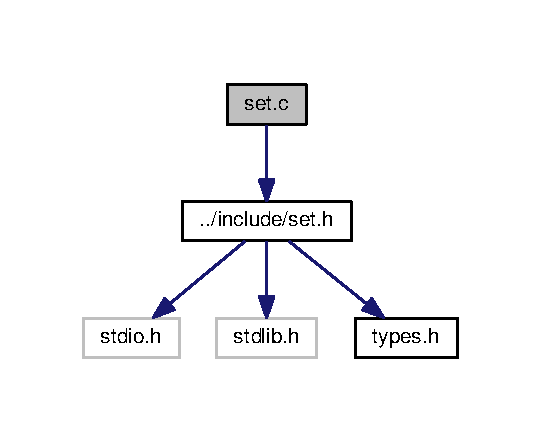
\includegraphics[width=260pt]{set_8c__incl}
\end{center}
\end{figure}
\subsection*{Classes}
\begin{DoxyCompactItemize}
\item 
struct \hyperlink{struct__Set}{\+\_\+\+Set}
\end{DoxyCompactItemize}
\subsection*{Functions}
\begin{DoxyCompactItemize}
\item 
\hyperlink{struct__Set}{Set} $\ast$ \hyperlink{set_8c_a34f3d3777fcb7f8b54b948527d4173b6}{set\+\_\+create} (int inv\+\_\+size)
\begin{DoxyCompactList}\small\item\em esta funcion se encarga de crear el conjunto reservando memoria para el mismo. \end{DoxyCompactList}\item 
void \hyperlink{set_8c_a9d762a027f1c3bcdd22f70ee9093a7dd}{set\+\_\+destroy} (\hyperlink{struct__Set}{Set} $\ast$set)
\begin{DoxyCompactList}\small\item\em esta funcion se encarga de destruir el conjunto. \end{DoxyCompactList}\item 
S\+T\+A\+T\+US \hyperlink{set_8c_a214235069ee276ad9bceb2c66e56bfe1}{set\+\_\+add} (\hyperlink{struct__Set}{Set} $\ast$set, Id id)
\begin{DoxyCompactList}\small\item\em esta funcion se encarga de añadir un elemento al conjunto. \end{DoxyCompactList}\item 
S\+T\+A\+T\+US \hyperlink{set_8c_a766d123b18af5298d23b51bc1ed433e6}{set\+\_\+del} (\hyperlink{struct__Set}{Set} $\ast$set, Id id)
\begin{DoxyCompactList}\small\item\em esta funcion se encarga de añadir un elemento al conjunto. \end{DoxyCompactList}\item 
Id \hyperlink{set_8c_ad882445dee89c289e8bcd971a56c2e55}{set\+\_\+get\+\_\+id} (\hyperlink{struct__Set}{Set} $\ast$set, int num)
\begin{DoxyCompactList}\small\item\em esta funcion se encarga de obtener el id de un conjunto. \end{DoxyCompactList}\item 
S\+T\+A\+T\+US \hyperlink{set_8c_aaa637b4dc68713c2e2c16ecda284d0aa}{set\+\_\+rm\+\_\+all} (\hyperlink{struct__Set}{Set} $\ast$set)
\begin{DoxyCompactList}\small\item\em esta funcion se encarga de vaciar el set, sin destruirlo \end{DoxyCompactList}\item 
\hyperlink{struct__Set}{Set} $\ast$ \hyperlink{set_8c_a8c1e1a34c5ab002443fda6efa9ba156f}{set\+\_\+cp\+\_\+all} (\hyperlink{struct__Set}{Set} $\ast$set)
\begin{DoxyCompactList}\small\item\em copia el set \end{DoxyCompactList}\item 
S\+T\+A\+T\+US \hyperlink{set_8c_a3ca7b2e04938630d7fd087975f15c162}{set\+\_\+rearrange} (\hyperlink{struct__Set}{Set} $\ast$set)
\begin{DoxyCompactList}\small\item\em limpia el set para que no haya espacios vacíos entre los llenos \end{DoxyCompactList}\item 
S\+T\+A\+T\+US \hyperlink{set_8c_ad26e71cbaea293d805f96d0644bcf80f}{set\+\_\+print\+\_\+debug} (F\+I\+LE $\ast$f, \hyperlink{struct__Set}{Set} $\ast$set)
\begin{DoxyCompactList}\small\item\em \mbox{[}D\+E\+B\+UG O\+N\+LY\mbox{]} imprime el set dado en el file dado \end{DoxyCompactList}\end{DoxyCompactItemize}


\subsection{Detailed Description}
Low level stack and queue functions. 

\begin{DoxyAuthor}{Author}
Bernardo Zambrano 
\end{DoxyAuthor}
\begin{DoxyCopyright}{Copyright}
G\+NU Public License 
\end{DoxyCopyright}


\subsection{Function Documentation}
\mbox{\Hypertarget{set_8c_a214235069ee276ad9bceb2c66e56bfe1}\label{set_8c_a214235069ee276ad9bceb2c66e56bfe1}} 
\index{set.\+c@{set.\+c}!set\+\_\+add@{set\+\_\+add}}
\index{set\+\_\+add@{set\+\_\+add}!set.\+c@{set.\+c}}
\subsubsection{\texorpdfstring{set\+\_\+add()}{set\_add()}}
{\footnotesize\ttfamily S\+T\+A\+T\+US set\+\_\+add (\begin{DoxyParamCaption}\item[{\hyperlink{struct__Set}{Set} $\ast$}]{,  }\item[{Id}]{ }\end{DoxyParamCaption})}



esta funcion se encarga de añadir un elemento al conjunto. 

\begin{DoxyAuthor}{Author}
Pablo Sánchez 
\end{DoxyAuthor}

\begin{DoxyParams}{Parameters}
{\em el} & conjunto donde se desea añadir el elemento. \\
\hline
{\em el} & id del elemento. \\
\hline
\end{DoxyParams}
\mbox{\Hypertarget{set_8c_a8c1e1a34c5ab002443fda6efa9ba156f}\label{set_8c_a8c1e1a34c5ab002443fda6efa9ba156f}} 
\index{set.\+c@{set.\+c}!set\+\_\+cp\+\_\+all@{set\+\_\+cp\+\_\+all}}
\index{set\+\_\+cp\+\_\+all@{set\+\_\+cp\+\_\+all}!set.\+c@{set.\+c}}
\subsubsection{\texorpdfstring{set\+\_\+cp\+\_\+all()}{set\_cp\_all()}}
{\footnotesize\ttfamily \hyperlink{struct__Set}{Set}$\ast$ set\+\_\+cp\+\_\+all (\begin{DoxyParamCaption}\item[{\hyperlink{struct__Set}{Set} $\ast$}]{ }\end{DoxyParamCaption})}



copia el set 

\begin{DoxyAuthor}{Author}
Antonio Solana  el set 
\end{DoxyAuthor}
\begin{DoxyReturn}{Returns}
copia del set 
\end{DoxyReturn}
\mbox{\Hypertarget{set_8c_a34f3d3777fcb7f8b54b948527d4173b6}\label{set_8c_a34f3d3777fcb7f8b54b948527d4173b6}} 
\index{set.\+c@{set.\+c}!set\+\_\+create@{set\+\_\+create}}
\index{set\+\_\+create@{set\+\_\+create}!set.\+c@{set.\+c}}
\subsubsection{\texorpdfstring{set\+\_\+create()}{set\_create()}}
{\footnotesize\ttfamily \hyperlink{struct__Set}{Set}$\ast$ set\+\_\+create (\begin{DoxyParamCaption}\item[{int}]{ }\end{DoxyParamCaption})}



esta funcion se encarga de crear el conjunto reservando memoria para el mismo. 

\begin{DoxyAuthor}{Author}
Pablo Sánchez 
\end{DoxyAuthor}
\begin{DoxyReturn}{Returns}
newset, el inventario creado, o N\+U\+LL si algo no ha salido como esperaba. 
\end{DoxyReturn}
\mbox{\Hypertarget{set_8c_a766d123b18af5298d23b51bc1ed433e6}\label{set_8c_a766d123b18af5298d23b51bc1ed433e6}} 
\index{set.\+c@{set.\+c}!set\+\_\+del@{set\+\_\+del}}
\index{set\+\_\+del@{set\+\_\+del}!set.\+c@{set.\+c}}
\subsubsection{\texorpdfstring{set\+\_\+del()}{set\_del()}}
{\footnotesize\ttfamily S\+T\+A\+T\+US set\+\_\+del (\begin{DoxyParamCaption}\item[{\hyperlink{struct__Set}{Set} $\ast$}]{,  }\item[{Id}]{ }\end{DoxyParamCaption})}



esta funcion se encarga de añadir un elemento al conjunto. 

\begin{DoxyAuthor}{Author}
Pablo Sánchez  el conjunto donde se desea añadir el elemento.  el id del elemento. 
\end{DoxyAuthor}
\mbox{\Hypertarget{set_8c_a9d762a027f1c3bcdd22f70ee9093a7dd}\label{set_8c_a9d762a027f1c3bcdd22f70ee9093a7dd}} 
\index{set.\+c@{set.\+c}!set\+\_\+destroy@{set\+\_\+destroy}}
\index{set\+\_\+destroy@{set\+\_\+destroy}!set.\+c@{set.\+c}}
\subsubsection{\texorpdfstring{set\+\_\+destroy()}{set\_destroy()}}
{\footnotesize\ttfamily void set\+\_\+destroy (\begin{DoxyParamCaption}\item[{\hyperlink{struct__Set}{Set} $\ast$}]{ }\end{DoxyParamCaption})}



esta funcion se encarga de destruir el conjunto. 

\begin{DoxyAuthor}{Author}
Pablo Sánchez 
\end{DoxyAuthor}

\begin{DoxyParams}{Parameters}
{\em el} & conjunto a destruir. \\
\hline
\end{DoxyParams}
\mbox{\Hypertarget{set_8c_ad882445dee89c289e8bcd971a56c2e55}\label{set_8c_ad882445dee89c289e8bcd971a56c2e55}} 
\index{set.\+c@{set.\+c}!set\+\_\+get\+\_\+id@{set\+\_\+get\+\_\+id}}
\index{set\+\_\+get\+\_\+id@{set\+\_\+get\+\_\+id}!set.\+c@{set.\+c}}
\subsubsection{\texorpdfstring{set\+\_\+get\+\_\+id()}{set\_get\_id()}}
{\footnotesize\ttfamily Id set\+\_\+get\+\_\+id (\begin{DoxyParamCaption}\item[{\hyperlink{struct__Set}{Set} $\ast$}]{,  }\item[{int}]{ }\end{DoxyParamCaption})}



esta funcion se encarga de obtener el id de un conjunto. 

\begin{DoxyAuthor}{Author}
Antonio Solana  el conjunto del cual se desea obtener la id 
\end{DoxyAuthor}
\begin{DoxyReturn}{Returns}
devuelve el id del conjunto. 
\end{DoxyReturn}
\mbox{\Hypertarget{set_8c_ad26e71cbaea293d805f96d0644bcf80f}\label{set_8c_ad26e71cbaea293d805f96d0644bcf80f}} 
\index{set.\+c@{set.\+c}!set\+\_\+print\+\_\+debug@{set\+\_\+print\+\_\+debug}}
\index{set\+\_\+print\+\_\+debug@{set\+\_\+print\+\_\+debug}!set.\+c@{set.\+c}}
\subsubsection{\texorpdfstring{set\+\_\+print\+\_\+debug()}{set\_print\_debug()}}
{\footnotesize\ttfamily S\+T\+A\+T\+US set\+\_\+print\+\_\+debug (\begin{DoxyParamCaption}\item[{F\+I\+LE $\ast$}]{,  }\item[{\hyperlink{struct__Set}{Set} $\ast$}]{ }\end{DoxyParamCaption})}



\mbox{[}D\+E\+B\+UG O\+N\+LY\mbox{]} imprime el set dado en el file dado 

\begin{DoxyAuthor}{Author}
Antonio Solana  el set, un lugar donde imprimir (debe estar abierto) 
\end{DoxyAuthor}
\begin{DoxyReturn}{Returns}
OK o E\+R\+R\+OR 
\end{DoxyReturn}
\mbox{\Hypertarget{set_8c_a3ca7b2e04938630d7fd087975f15c162}\label{set_8c_a3ca7b2e04938630d7fd087975f15c162}} 
\index{set.\+c@{set.\+c}!set\+\_\+rearrange@{set\+\_\+rearrange}}
\index{set\+\_\+rearrange@{set\+\_\+rearrange}!set.\+c@{set.\+c}}
\subsubsection{\texorpdfstring{set\+\_\+rearrange()}{set\_rearrange()}}
{\footnotesize\ttfamily S\+T\+A\+T\+US set\+\_\+rearrange (\begin{DoxyParamCaption}\item[{\hyperlink{struct__Set}{Set} $\ast$}]{ }\end{DoxyParamCaption})}



limpia el set para que no haya espacios vacíos entre los llenos 

\begin{DoxyAuthor}{Author}
Antonio Solana  el set 
\end{DoxyAuthor}
\begin{DoxyReturn}{Returns}
OK o E\+R\+R\+OR 
\end{DoxyReturn}
\mbox{\Hypertarget{set_8c_aaa637b4dc68713c2e2c16ecda284d0aa}\label{set_8c_aaa637b4dc68713c2e2c16ecda284d0aa}} 
\index{set.\+c@{set.\+c}!set\+\_\+rm\+\_\+all@{set\+\_\+rm\+\_\+all}}
\index{set\+\_\+rm\+\_\+all@{set\+\_\+rm\+\_\+all}!set.\+c@{set.\+c}}
\subsubsection{\texorpdfstring{set\+\_\+rm\+\_\+all()}{set\_rm\_all()}}
{\footnotesize\ttfamily S\+T\+A\+T\+US set\+\_\+rm\+\_\+all (\begin{DoxyParamCaption}\item[{\hyperlink{struct__Set}{Set} $\ast$}]{ }\end{DoxyParamCaption})}



esta funcion se encarga de vaciar el set, sin destruirlo 

\begin{DoxyAuthor}{Author}
Antonio Solana  el set 
\end{DoxyAuthor}
\begin{DoxyReturn}{Returns}
OK o E\+R\+R\+OR 
\end{DoxyReturn}

\hypertarget{set_8h}{\section{set.\+h File Reference}
\label{set_8h}\index{set.\+h@{set.\+h}}
}


Low level stack and queue functions.  


{\ttfamily \#include $<$stdio.\+h$>$}\\*
{\ttfamily \#include $<$stdlib.\+h$>$}\\*
{\ttfamily \#include \char`\"{}types.\+h\char`\"{}}\\*
Include dependency graph for set.\+h\+:\nopagebreak
\begin{figure}[H]
\begin{center}
\leavevmode
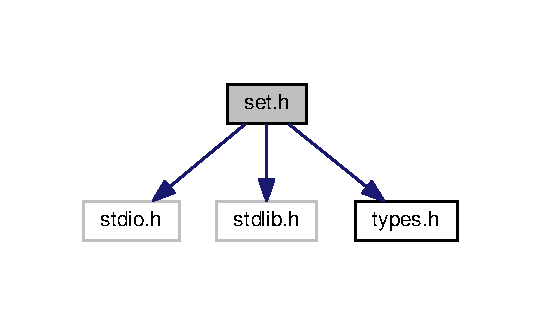
\includegraphics[width=259pt]{set_8h__incl}
\end{center}
\end{figure}
This graph shows which files directly or indirectly include this file\+:\nopagebreak
\begin{figure}[H]
\begin{center}
\leavevmode
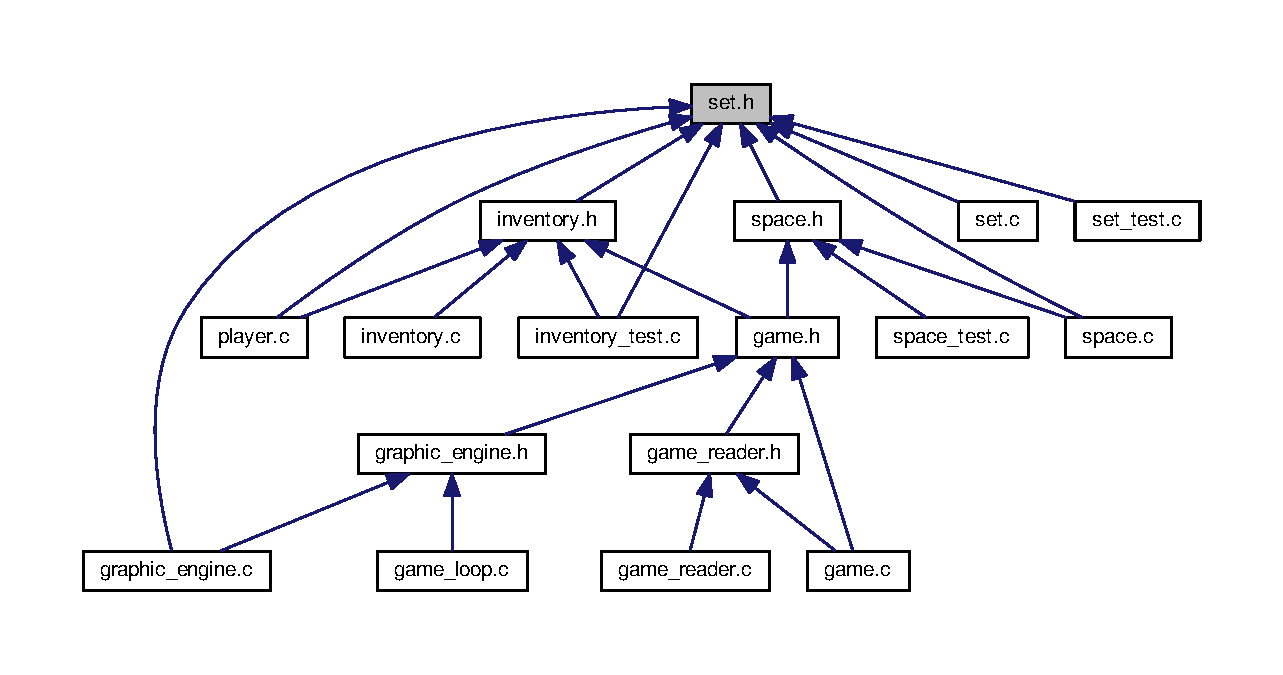
\includegraphics[width=350pt]{set_8h__dep__incl}
\end{center}
\end{figure}
\subsection*{Macros}
\begin{DoxyCompactItemize}
\item 
\#define \hyperlink{set_8h_af6e65f998f2940aaf745740214a3facf}{M\+A\+X\+\_\+\+I\+N\+V\+\_\+\+S\+I\+Z\+E}~1024
\end{DoxyCompactItemize}
\subsection*{Typedefs}
\begin{DoxyCompactItemize}
\item 
typedef struct \hyperlink{struct__Set}{\+\_\+\+Set} \hyperlink{set_8h_a6d3b7f7c92cbb4577ef3ef7ddbf93161}{Set}
\end{DoxyCompactItemize}
\subsection*{Functions}
\begin{DoxyCompactItemize}
\item 
\hyperlink{set_8h_a6d3b7f7c92cbb4577ef3ef7ddbf93161}{Set} $\ast$ \hyperlink{set_8h_a7c15d7dafaced1962d30497909553230}{set\+\_\+create} (int)
\item 
void \hyperlink{set_8h_a4bf32e87a700bb58fb2ce374207049ab}{set\+\_\+destroy} (\hyperlink{set_8h_a6d3b7f7c92cbb4577ef3ef7ddbf93161}{Set} $\ast$)
\item 
\hyperlink{types_8h_a32c27cc471df37f4fc818d65de0a56c4}{S\+T\+A\+T\+U\+S} \hyperlink{set_8h_ada6e5ed947e3b64276501c5337676fba}{set\+\_\+add} (\hyperlink{set_8h_a6d3b7f7c92cbb4577ef3ef7ddbf93161}{Set} $\ast$, \hyperlink{types_8h_a845e604fb28f7e3d97549da3448149d3}{Id})
\item 
\hyperlink{types_8h_a32c27cc471df37f4fc818d65de0a56c4}{S\+T\+A\+T\+U\+S} \hyperlink{set_8h_a0f85803b8c26d13d756ef04bbc0e5b75}{set\+\_\+del} (\hyperlink{set_8h_a6d3b7f7c92cbb4577ef3ef7ddbf93161}{Set} $\ast$, \hyperlink{types_8h_a845e604fb28f7e3d97549da3448149d3}{Id})
\item 
\hyperlink{types_8h_a845e604fb28f7e3d97549da3448149d3}{Id} \hyperlink{set_8h_a3b3a798e2254fdbf80a631e37f490311}{set\+\_\+get\+\_\+id} (\hyperlink{set_8h_a6d3b7f7c92cbb4577ef3ef7ddbf93161}{Set} $\ast$, int)
\item 
\hyperlink{types_8h_a32c27cc471df37f4fc818d65de0a56c4}{S\+T\+A\+T\+U\+S} \hyperlink{set_8h_a4a47e3f4883568f27b96635922aae920}{set\+\_\+rm\+\_\+all} (\hyperlink{set_8h_a6d3b7f7c92cbb4577ef3ef7ddbf93161}{Set} $\ast$)
\item 
\hyperlink{types_8h_a32c27cc471df37f4fc818d65de0a56c4}{S\+T\+A\+T\+U\+S} \hyperlink{set_8h_af93e66655e2d02642666112e76d8a708}{set\+\_\+rearrange} (\hyperlink{set_8h_a6d3b7f7c92cbb4577ef3ef7ddbf93161}{Set} $\ast$)
\item 
\hyperlink{set_8h_a6d3b7f7c92cbb4577ef3ef7ddbf93161}{Set} $\ast$ \hyperlink{set_8h_a4fb1df6e6b413fac7edba6c3af5b39f7}{set\+\_\+cp\+\_\+all} (\hyperlink{set_8h_a6d3b7f7c92cbb4577ef3ef7ddbf93161}{Set} $\ast$)
\item 
\hyperlink{types_8h_a32c27cc471df37f4fc818d65de0a56c4}{S\+T\+A\+T\+U\+S} \hyperlink{set_8h_ad3f81629d9a22cdfc7721f5d92f0232f}{set\+\_\+print\+\_\+debug} (F\+I\+L\+E $\ast$, \hyperlink{set_8h_a6d3b7f7c92cbb4577ef3ef7ddbf93161}{Set} $\ast$)
\end{DoxyCompactItemize}


\subsection{Detailed Description}
Low level stack and queue functions. 

\begin{DoxyAuthor}{Author}
Bernardo Zambrano 
\end{DoxyAuthor}
\begin{DoxyCopyright}{Copyright}
G\+N\+U Public License 
\end{DoxyCopyright}


\subsection{Macro Definition Documentation}
\hypertarget{set_8h_af6e65f998f2940aaf745740214a3facf}{\index{set.\+h@{set.\+h}!M\+A\+X\+\_\+\+I\+N\+V\+\_\+\+S\+I\+Z\+E@{M\+A\+X\+\_\+\+I\+N\+V\+\_\+\+S\+I\+Z\+E}}
\index{M\+A\+X\+\_\+\+I\+N\+V\+\_\+\+S\+I\+Z\+E@{M\+A\+X\+\_\+\+I\+N\+V\+\_\+\+S\+I\+Z\+E}!set.\+h@{set.\+h}}
\subsubsection[{M\+A\+X\+\_\+\+I\+N\+V\+\_\+\+S\+I\+Z\+E}]{\setlength{\rightskip}{0pt plus 5cm}\#define M\+A\+X\+\_\+\+I\+N\+V\+\_\+\+S\+I\+Z\+E~1024}}\label{set_8h_af6e65f998f2940aaf745740214a3facf}


\subsection{Typedef Documentation}
\hypertarget{set_8h_a6d3b7f7c92cbb4577ef3ef7ddbf93161}{\index{set.\+h@{set.\+h}!Set@{Set}}
\index{Set@{Set}!set.\+h@{set.\+h}}
\subsubsection[{Set}]{\setlength{\rightskip}{0pt plus 5cm}typedef struct {\bf \+\_\+\+Set} {\bf Set}}}\label{set_8h_a6d3b7f7c92cbb4577ef3ef7ddbf93161}


\subsection{Function Documentation}
\hypertarget{set_8h_ada6e5ed947e3b64276501c5337676fba}{\index{set.\+h@{set.\+h}!set\+\_\+add@{set\+\_\+add}}
\index{set\+\_\+add@{set\+\_\+add}!set.\+h@{set.\+h}}
\subsubsection[{set\+\_\+add}]{\setlength{\rightskip}{0pt plus 5cm}{\bf S\+T\+A\+T\+U\+S} set\+\_\+add (
\begin{DoxyParamCaption}
\item[{{\bf Set} $\ast$}]{, }
\item[{{\bf Id}}]{}
\end{DoxyParamCaption}
)}}\label{set_8h_ada6e5ed947e3b64276501c5337676fba}
\hypertarget{set_8h_a4fb1df6e6b413fac7edba6c3af5b39f7}{\index{set.\+h@{set.\+h}!set\+\_\+cp\+\_\+all@{set\+\_\+cp\+\_\+all}}
\index{set\+\_\+cp\+\_\+all@{set\+\_\+cp\+\_\+all}!set.\+h@{set.\+h}}
\subsubsection[{set\+\_\+cp\+\_\+all}]{\setlength{\rightskip}{0pt plus 5cm}{\bf Set}$\ast$ set\+\_\+cp\+\_\+all (
\begin{DoxyParamCaption}
\item[{{\bf Set} $\ast$}]{}
\end{DoxyParamCaption}
)}}\label{set_8h_a4fb1df6e6b413fac7edba6c3af5b39f7}
\hypertarget{set_8h_a7c15d7dafaced1962d30497909553230}{\index{set.\+h@{set.\+h}!set\+\_\+create@{set\+\_\+create}}
\index{set\+\_\+create@{set\+\_\+create}!set.\+h@{set.\+h}}
\subsubsection[{set\+\_\+create}]{\setlength{\rightskip}{0pt plus 5cm}{\bf Set}$\ast$ set\+\_\+create (
\begin{DoxyParamCaption}
\item[{int}]{}
\end{DoxyParamCaption}
)}}\label{set_8h_a7c15d7dafaced1962d30497909553230}
\hypertarget{set_8h_a0f85803b8c26d13d756ef04bbc0e5b75}{\index{set.\+h@{set.\+h}!set\+\_\+del@{set\+\_\+del}}
\index{set\+\_\+del@{set\+\_\+del}!set.\+h@{set.\+h}}
\subsubsection[{set\+\_\+del}]{\setlength{\rightskip}{0pt plus 5cm}{\bf S\+T\+A\+T\+U\+S} set\+\_\+del (
\begin{DoxyParamCaption}
\item[{{\bf Set} $\ast$}]{, }
\item[{{\bf Id}}]{}
\end{DoxyParamCaption}
)}}\label{set_8h_a0f85803b8c26d13d756ef04bbc0e5b75}
\hypertarget{set_8h_a4bf32e87a700bb58fb2ce374207049ab}{\index{set.\+h@{set.\+h}!set\+\_\+destroy@{set\+\_\+destroy}}
\index{set\+\_\+destroy@{set\+\_\+destroy}!set.\+h@{set.\+h}}
\subsubsection[{set\+\_\+destroy}]{\setlength{\rightskip}{0pt plus 5cm}void set\+\_\+destroy (
\begin{DoxyParamCaption}
\item[{{\bf Set} $\ast$}]{}
\end{DoxyParamCaption}
)}}\label{set_8h_a4bf32e87a700bb58fb2ce374207049ab}
\hypertarget{set_8h_a3b3a798e2254fdbf80a631e37f490311}{\index{set.\+h@{set.\+h}!set\+\_\+get\+\_\+id@{set\+\_\+get\+\_\+id}}
\index{set\+\_\+get\+\_\+id@{set\+\_\+get\+\_\+id}!set.\+h@{set.\+h}}
\subsubsection[{set\+\_\+get\+\_\+id}]{\setlength{\rightskip}{0pt plus 5cm}{\bf Id} set\+\_\+get\+\_\+id (
\begin{DoxyParamCaption}
\item[{{\bf Set} $\ast$}]{, }
\item[{int}]{}
\end{DoxyParamCaption}
)}}\label{set_8h_a3b3a798e2254fdbf80a631e37f490311}
\hypertarget{set_8h_ad3f81629d9a22cdfc7721f5d92f0232f}{\index{set.\+h@{set.\+h}!set\+\_\+print\+\_\+debug@{set\+\_\+print\+\_\+debug}}
\index{set\+\_\+print\+\_\+debug@{set\+\_\+print\+\_\+debug}!set.\+h@{set.\+h}}
\subsubsection[{set\+\_\+print\+\_\+debug}]{\setlength{\rightskip}{0pt plus 5cm}{\bf S\+T\+A\+T\+U\+S} set\+\_\+print\+\_\+debug (
\begin{DoxyParamCaption}
\item[{F\+I\+L\+E $\ast$}]{, }
\item[{{\bf Set} $\ast$}]{}
\end{DoxyParamCaption}
)}}\label{set_8h_ad3f81629d9a22cdfc7721f5d92f0232f}
\hypertarget{set_8h_af93e66655e2d02642666112e76d8a708}{\index{set.\+h@{set.\+h}!set\+\_\+rearrange@{set\+\_\+rearrange}}
\index{set\+\_\+rearrange@{set\+\_\+rearrange}!set.\+h@{set.\+h}}
\subsubsection[{set\+\_\+rearrange}]{\setlength{\rightskip}{0pt plus 5cm}{\bf S\+T\+A\+T\+U\+S} set\+\_\+rearrange (
\begin{DoxyParamCaption}
\item[{{\bf Set} $\ast$}]{}
\end{DoxyParamCaption}
)}}\label{set_8h_af93e66655e2d02642666112e76d8a708}
\hypertarget{set_8h_a4a47e3f4883568f27b96635922aae920}{\index{set.\+h@{set.\+h}!set\+\_\+rm\+\_\+all@{set\+\_\+rm\+\_\+all}}
\index{set\+\_\+rm\+\_\+all@{set\+\_\+rm\+\_\+all}!set.\+h@{set.\+h}}
\subsubsection[{set\+\_\+rm\+\_\+all}]{\setlength{\rightskip}{0pt plus 5cm}{\bf S\+T\+A\+T\+U\+S} set\+\_\+rm\+\_\+all (
\begin{DoxyParamCaption}
\item[{{\bf Set} $\ast$}]{}
\end{DoxyParamCaption}
)}}\label{set_8h_a4a47e3f4883568f27b96635922aae920}

\hypertarget{set__test_8c}{}\section{set\+\_\+test.\+c File Reference}
\label{set__test_8c}\index{set\+\_\+test.\+c@{set\+\_\+test.\+c}}
{\ttfamily \#include $<$stdio.\+h$>$}\\*
{\ttfamily \#include $<$stdlib.\+h$>$}\\*
{\ttfamily \#include $<$string.\+h$>$}\\*
{\ttfamily \#include \char`\"{}../include/set.\+h\char`\"{}}\\*
{\ttfamily \#include \char`\"{}../include/set\+\_\+test.\+h\char`\"{}}\\*
{\ttfamily \#include \char`\"{}../include/test.\+h\char`\"{}}\\*
Include dependency graph for set\+\_\+test.\+c\+:\nopagebreak
\begin{figure}[H]
\begin{center}
\leavevmode
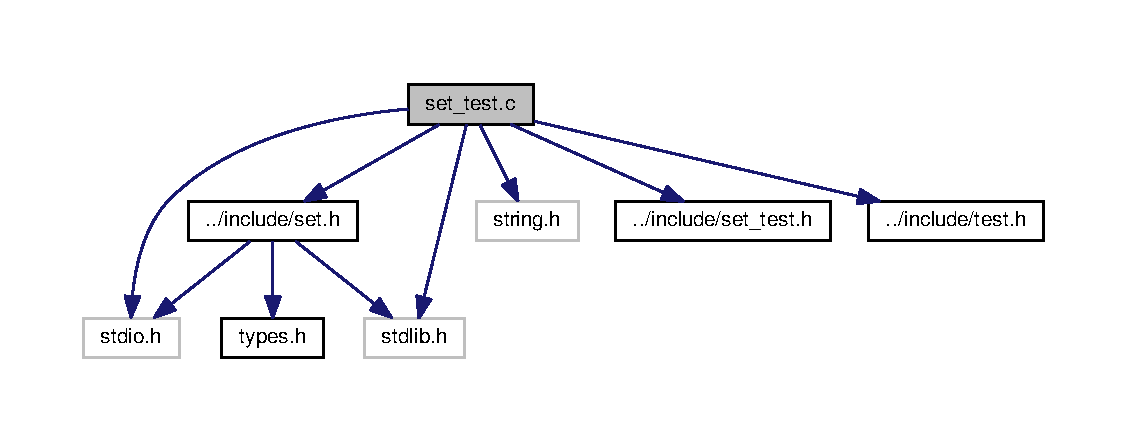
\includegraphics[width=350pt]{set__test_8c__incl}
\end{center}
\end{figure}
\subsection*{Macros}
\begin{DoxyCompactItemize}
\item 
\#define \hyperlink{set__test_8c_a2a77d2f2c5b698c69c19e1f8782bf709}{M\+A\+X\+\_\+\+T\+E\+S\+TS}~28
\end{DoxyCompactItemize}
\subsection*{Functions}
\begin{DoxyCompactItemize}
\item 
int \hyperlink{set__test_8c_a3c04138a5bfe5d72780bb7e82a18e627}{main} (int argc, char $\ast$$\ast$argv)
\begin{DoxyCompactList}\small\item\em Funcion principal de pruebas para el modulo Space. \end{DoxyCompactList}\item 
void \hyperlink{set__test_8c_a6f654ab4b44e8a9b9cedfb78c378a5d7}{test1\+\_\+set\+\_\+create} ()
\item 
void \hyperlink{set__test_8c_a014ebe1b46af5ea318143fc61894d9c0}{test1\+\_\+set\+\_\+add} ()
\item 
void \hyperlink{set__test_8c_ab09827322a313bf97b9757c98c2bdbb0}{test2\+\_\+set\+\_\+add} ()
\item 
void \hyperlink{set__test_8c_a2a15d0c24e7a943dec28b6d8e3850e60}{test1\+\_\+set\+\_\+del} ()
\item 
void \hyperlink{set__test_8c_a4e8b8663f067122ea82b83e2d07e685c}{test2\+\_\+set\+\_\+del} ()
\item 
void \hyperlink{set__test_8c_af5b80896afe0d23ab4a347bdb4b3c48b}{test1\+\_\+set\+\_\+get\+\_\+id} ()
\item 
void \hyperlink{set__test_8c_a665b83794eafe832cc4d71aa42dc016d}{test2\+\_\+set\+\_\+get\+\_\+id} ()
\item 
void \hyperlink{set__test_8c_a88f5ed9ffd44c08fd4e08c647506c257}{test1\+\_\+set\+\_\+rm\+\_\+all} ()
\item 
void \hyperlink{set__test_8c_a5e7078d4972370c0b06618b514787b6c}{test2\+\_\+set\+\_\+rm\+\_\+all} ()
\item 
void \hyperlink{set__test_8c_a445dfce2dcca32a9454205ae4a3d6007}{test1\+\_\+set\+\_\+rearrange} ()
\item 
void \hyperlink{set__test_8c_ab2697b95104977c543087493a26dd39b}{test2\+\_\+set\+\_\+rearrange} ()
\item 
void \hyperlink{set__test_8c_af935827bf3ef10631736d720e41afd9d}{test1\+\_\+set\+\_\+cp\+\_\+all} ()
\item 
void \hyperlink{set__test_8c_ab8754ea8f52366f761911b6b0db2c0f6}{test2\+\_\+set\+\_\+cp\+\_\+all} ()
\end{DoxyCompactItemize}


\subsection{Macro Definition Documentation}
\index{set\+\_\+test.\+c@{set\+\_\+test.\+c}!M\+A\+X\+\_\+\+T\+E\+S\+TS@{M\+A\+X\+\_\+\+T\+E\+S\+TS}}
\index{M\+A\+X\+\_\+\+T\+E\+S\+TS@{M\+A\+X\+\_\+\+T\+E\+S\+TS}!set\+\_\+test.\+c@{set\+\_\+test.\+c}}
\subsubsection[{\texorpdfstring{M\+A\+X\+\_\+\+T\+E\+S\+TS}{MAX_TESTS}}]{\setlength{\rightskip}{0pt plus 5cm}\#define M\+A\+X\+\_\+\+T\+E\+S\+TS~28}\hypertarget{set__test_8c_a2a77d2f2c5b698c69c19e1f8782bf709}{}\label{set__test_8c_a2a77d2f2c5b698c69c19e1f8782bf709}


\subsection{Function Documentation}
\index{set\+\_\+test.\+c@{set\+\_\+test.\+c}!main@{main}}
\index{main@{main}!set\+\_\+test.\+c@{set\+\_\+test.\+c}}
\subsubsection[{\texorpdfstring{main(int argc, char $\ast$$\ast$argv)}{main(int argc, char **argv)}}]{\setlength{\rightskip}{0pt plus 5cm}int main (
\begin{DoxyParamCaption}
\item[{int}]{argc, }
\item[{char $\ast$$\ast$}]{argv}
\end{DoxyParamCaption}
)}\hypertarget{set__test_8c_a3c04138a5bfe5d72780bb7e82a18e627}{}\label{set__test_8c_a3c04138a5bfe5d72780bb7e82a18e627}


Funcion principal de pruebas para el modulo Space. 

Dos modos de ejecucion\+: 1.-\/\+Si se ejecuta sin parametros se ejecutan todas las pruebas 2.-\/\+Si se ejecuta con un numero entre 1 y el numero de pruebas solo ejecuta la prueba indicada \index{set\+\_\+test.\+c@{set\+\_\+test.\+c}!test1\+\_\+set\+\_\+add@{test1\+\_\+set\+\_\+add}}
\index{test1\+\_\+set\+\_\+add@{test1\+\_\+set\+\_\+add}!set\+\_\+test.\+c@{set\+\_\+test.\+c}}
\subsubsection[{\texorpdfstring{test1\+\_\+set\+\_\+add()}{test1_set_add()}}]{\setlength{\rightskip}{0pt plus 5cm}void test1\+\_\+set\+\_\+add (
\begin{DoxyParamCaption}
{}
\end{DoxyParamCaption}
)}\hypertarget{set__test_8c_a014ebe1b46af5ea318143fc61894d9c0}{}\label{set__test_8c_a014ebe1b46af5ea318143fc61894d9c0}
\index{set\+\_\+test.\+c@{set\+\_\+test.\+c}!test1\+\_\+set\+\_\+cp\+\_\+all@{test1\+\_\+set\+\_\+cp\+\_\+all}}
\index{test1\+\_\+set\+\_\+cp\+\_\+all@{test1\+\_\+set\+\_\+cp\+\_\+all}!set\+\_\+test.\+c@{set\+\_\+test.\+c}}
\subsubsection[{\texorpdfstring{test1\+\_\+set\+\_\+cp\+\_\+all()}{test1_set_cp_all()}}]{\setlength{\rightskip}{0pt plus 5cm}void test1\+\_\+set\+\_\+cp\+\_\+all (
\begin{DoxyParamCaption}
{}
\end{DoxyParamCaption}
)}\hypertarget{set__test_8c_af935827bf3ef10631736d720e41afd9d}{}\label{set__test_8c_af935827bf3ef10631736d720e41afd9d}
\index{set\+\_\+test.\+c@{set\+\_\+test.\+c}!test1\+\_\+set\+\_\+create@{test1\+\_\+set\+\_\+create}}
\index{test1\+\_\+set\+\_\+create@{test1\+\_\+set\+\_\+create}!set\+\_\+test.\+c@{set\+\_\+test.\+c}}
\subsubsection[{\texorpdfstring{test1\+\_\+set\+\_\+create()}{test1_set_create()}}]{\setlength{\rightskip}{0pt plus 5cm}void test1\+\_\+set\+\_\+create (
\begin{DoxyParamCaption}
{}
\end{DoxyParamCaption}
)}\hypertarget{set__test_8c_a6f654ab4b44e8a9b9cedfb78c378a5d7}{}\label{set__test_8c_a6f654ab4b44e8a9b9cedfb78c378a5d7}
\index{set\+\_\+test.\+c@{set\+\_\+test.\+c}!test1\+\_\+set\+\_\+del@{test1\+\_\+set\+\_\+del}}
\index{test1\+\_\+set\+\_\+del@{test1\+\_\+set\+\_\+del}!set\+\_\+test.\+c@{set\+\_\+test.\+c}}
\subsubsection[{\texorpdfstring{test1\+\_\+set\+\_\+del()}{test1_set_del()}}]{\setlength{\rightskip}{0pt plus 5cm}void test1\+\_\+set\+\_\+del (
\begin{DoxyParamCaption}
{}
\end{DoxyParamCaption}
)}\hypertarget{set__test_8c_a2a15d0c24e7a943dec28b6d8e3850e60}{}\label{set__test_8c_a2a15d0c24e7a943dec28b6d8e3850e60}
\index{set\+\_\+test.\+c@{set\+\_\+test.\+c}!test1\+\_\+set\+\_\+get\+\_\+id@{test1\+\_\+set\+\_\+get\+\_\+id}}
\index{test1\+\_\+set\+\_\+get\+\_\+id@{test1\+\_\+set\+\_\+get\+\_\+id}!set\+\_\+test.\+c@{set\+\_\+test.\+c}}
\subsubsection[{\texorpdfstring{test1\+\_\+set\+\_\+get\+\_\+id()}{test1_set_get_id()}}]{\setlength{\rightskip}{0pt plus 5cm}void test1\+\_\+set\+\_\+get\+\_\+id (
\begin{DoxyParamCaption}
{}
\end{DoxyParamCaption}
)}\hypertarget{set__test_8c_af5b80896afe0d23ab4a347bdb4b3c48b}{}\label{set__test_8c_af5b80896afe0d23ab4a347bdb4b3c48b}
\index{set\+\_\+test.\+c@{set\+\_\+test.\+c}!test1\+\_\+set\+\_\+rearrange@{test1\+\_\+set\+\_\+rearrange}}
\index{test1\+\_\+set\+\_\+rearrange@{test1\+\_\+set\+\_\+rearrange}!set\+\_\+test.\+c@{set\+\_\+test.\+c}}
\subsubsection[{\texorpdfstring{test1\+\_\+set\+\_\+rearrange()}{test1_set_rearrange()}}]{\setlength{\rightskip}{0pt plus 5cm}void test1\+\_\+set\+\_\+rearrange (
\begin{DoxyParamCaption}
{}
\end{DoxyParamCaption}
)}\hypertarget{set__test_8c_a445dfce2dcca32a9454205ae4a3d6007}{}\label{set__test_8c_a445dfce2dcca32a9454205ae4a3d6007}
\index{set\+\_\+test.\+c@{set\+\_\+test.\+c}!test1\+\_\+set\+\_\+rm\+\_\+all@{test1\+\_\+set\+\_\+rm\+\_\+all}}
\index{test1\+\_\+set\+\_\+rm\+\_\+all@{test1\+\_\+set\+\_\+rm\+\_\+all}!set\+\_\+test.\+c@{set\+\_\+test.\+c}}
\subsubsection[{\texorpdfstring{test1\+\_\+set\+\_\+rm\+\_\+all()}{test1_set_rm_all()}}]{\setlength{\rightskip}{0pt plus 5cm}void test1\+\_\+set\+\_\+rm\+\_\+all (
\begin{DoxyParamCaption}
{}
\end{DoxyParamCaption}
)}\hypertarget{set__test_8c_a88f5ed9ffd44c08fd4e08c647506c257}{}\label{set__test_8c_a88f5ed9ffd44c08fd4e08c647506c257}
\index{set\+\_\+test.\+c@{set\+\_\+test.\+c}!test2\+\_\+set\+\_\+add@{test2\+\_\+set\+\_\+add}}
\index{test2\+\_\+set\+\_\+add@{test2\+\_\+set\+\_\+add}!set\+\_\+test.\+c@{set\+\_\+test.\+c}}
\subsubsection[{\texorpdfstring{test2\+\_\+set\+\_\+add()}{test2_set_add()}}]{\setlength{\rightskip}{0pt plus 5cm}void test2\+\_\+set\+\_\+add (
\begin{DoxyParamCaption}
{}
\end{DoxyParamCaption}
)}\hypertarget{set__test_8c_ab09827322a313bf97b9757c98c2bdbb0}{}\label{set__test_8c_ab09827322a313bf97b9757c98c2bdbb0}
\index{set\+\_\+test.\+c@{set\+\_\+test.\+c}!test2\+\_\+set\+\_\+cp\+\_\+all@{test2\+\_\+set\+\_\+cp\+\_\+all}}
\index{test2\+\_\+set\+\_\+cp\+\_\+all@{test2\+\_\+set\+\_\+cp\+\_\+all}!set\+\_\+test.\+c@{set\+\_\+test.\+c}}
\subsubsection[{\texorpdfstring{test2\+\_\+set\+\_\+cp\+\_\+all()}{test2_set_cp_all()}}]{\setlength{\rightskip}{0pt plus 5cm}void test2\+\_\+set\+\_\+cp\+\_\+all (
\begin{DoxyParamCaption}
{}
\end{DoxyParamCaption}
)}\hypertarget{set__test_8c_ab8754ea8f52366f761911b6b0db2c0f6}{}\label{set__test_8c_ab8754ea8f52366f761911b6b0db2c0f6}
\index{set\+\_\+test.\+c@{set\+\_\+test.\+c}!test2\+\_\+set\+\_\+del@{test2\+\_\+set\+\_\+del}}
\index{test2\+\_\+set\+\_\+del@{test2\+\_\+set\+\_\+del}!set\+\_\+test.\+c@{set\+\_\+test.\+c}}
\subsubsection[{\texorpdfstring{test2\+\_\+set\+\_\+del()}{test2_set_del()}}]{\setlength{\rightskip}{0pt plus 5cm}void test2\+\_\+set\+\_\+del (
\begin{DoxyParamCaption}
{}
\end{DoxyParamCaption}
)}\hypertarget{set__test_8c_a4e8b8663f067122ea82b83e2d07e685c}{}\label{set__test_8c_a4e8b8663f067122ea82b83e2d07e685c}
\index{set\+\_\+test.\+c@{set\+\_\+test.\+c}!test2\+\_\+set\+\_\+get\+\_\+id@{test2\+\_\+set\+\_\+get\+\_\+id}}
\index{test2\+\_\+set\+\_\+get\+\_\+id@{test2\+\_\+set\+\_\+get\+\_\+id}!set\+\_\+test.\+c@{set\+\_\+test.\+c}}
\subsubsection[{\texorpdfstring{test2\+\_\+set\+\_\+get\+\_\+id()}{test2_set_get_id()}}]{\setlength{\rightskip}{0pt plus 5cm}void test2\+\_\+set\+\_\+get\+\_\+id (
\begin{DoxyParamCaption}
{}
\end{DoxyParamCaption}
)}\hypertarget{set__test_8c_a665b83794eafe832cc4d71aa42dc016d}{}\label{set__test_8c_a665b83794eafe832cc4d71aa42dc016d}
\index{set\+\_\+test.\+c@{set\+\_\+test.\+c}!test2\+\_\+set\+\_\+rearrange@{test2\+\_\+set\+\_\+rearrange}}
\index{test2\+\_\+set\+\_\+rearrange@{test2\+\_\+set\+\_\+rearrange}!set\+\_\+test.\+c@{set\+\_\+test.\+c}}
\subsubsection[{\texorpdfstring{test2\+\_\+set\+\_\+rearrange()}{test2_set_rearrange()}}]{\setlength{\rightskip}{0pt plus 5cm}void test2\+\_\+set\+\_\+rearrange (
\begin{DoxyParamCaption}
{}
\end{DoxyParamCaption}
)}\hypertarget{set__test_8c_ab2697b95104977c543087493a26dd39b}{}\label{set__test_8c_ab2697b95104977c543087493a26dd39b}
\index{set\+\_\+test.\+c@{set\+\_\+test.\+c}!test2\+\_\+set\+\_\+rm\+\_\+all@{test2\+\_\+set\+\_\+rm\+\_\+all}}
\index{test2\+\_\+set\+\_\+rm\+\_\+all@{test2\+\_\+set\+\_\+rm\+\_\+all}!set\+\_\+test.\+c@{set\+\_\+test.\+c}}
\subsubsection[{\texorpdfstring{test2\+\_\+set\+\_\+rm\+\_\+all()}{test2_set_rm_all()}}]{\setlength{\rightskip}{0pt plus 5cm}void test2\+\_\+set\+\_\+rm\+\_\+all (
\begin{DoxyParamCaption}
{}
\end{DoxyParamCaption}
)}\hypertarget{set__test_8c_a5e7078d4972370c0b06618b514787b6c}{}\label{set__test_8c_a5e7078d4972370c0b06618b514787b6c}

\hypertarget{set__test_8h}{}\section{include/set\+\_\+test.h File Reference}
\label{set__test_8h}\index{include/set\+\_\+test.\+h@{include/set\+\_\+test.\+h}}


It declares the tests for the set module.  


\subsection*{Functions}
\begin{DoxyCompactItemize}
\item 
\mbox{\Hypertarget{set__test_8h_a6f654ab4b44e8a9b9cedfb78c378a5d7}\label{set__test_8h_a6f654ab4b44e8a9b9cedfb78c378a5d7}} 
void {\bfseries test1\+\_\+set\+\_\+create} ()
\item 
\mbox{\Hypertarget{set__test_8h_a014ebe1b46af5ea318143fc61894d9c0}\label{set__test_8h_a014ebe1b46af5ea318143fc61894d9c0}} 
void {\bfseries test1\+\_\+set\+\_\+add} ()
\item 
\mbox{\Hypertarget{set__test_8h_ab09827322a313bf97b9757c98c2bdbb0}\label{set__test_8h_ab09827322a313bf97b9757c98c2bdbb0}} 
void {\bfseries test2\+\_\+set\+\_\+add} ()
\item 
\mbox{\Hypertarget{set__test_8h_a2a15d0c24e7a943dec28b6d8e3850e60}\label{set__test_8h_a2a15d0c24e7a943dec28b6d8e3850e60}} 
void {\bfseries test1\+\_\+set\+\_\+del} ()
\item 
\mbox{\Hypertarget{set__test_8h_a4e8b8663f067122ea82b83e2d07e685c}\label{set__test_8h_a4e8b8663f067122ea82b83e2d07e685c}} 
void {\bfseries test2\+\_\+set\+\_\+del} ()
\item 
\mbox{\Hypertarget{set__test_8h_af5b80896afe0d23ab4a347bdb4b3c48b}\label{set__test_8h_af5b80896afe0d23ab4a347bdb4b3c48b}} 
void {\bfseries test1\+\_\+set\+\_\+get\+\_\+id} ()
\item 
\mbox{\Hypertarget{set__test_8h_a665b83794eafe832cc4d71aa42dc016d}\label{set__test_8h_a665b83794eafe832cc4d71aa42dc016d}} 
void {\bfseries test2\+\_\+set\+\_\+get\+\_\+id} ()
\item 
\mbox{\Hypertarget{set__test_8h_a88f5ed9ffd44c08fd4e08c647506c257}\label{set__test_8h_a88f5ed9ffd44c08fd4e08c647506c257}} 
void {\bfseries test1\+\_\+set\+\_\+rm\+\_\+all} ()
\item 
\mbox{\Hypertarget{set__test_8h_a5e7078d4972370c0b06618b514787b6c}\label{set__test_8h_a5e7078d4972370c0b06618b514787b6c}} 
void {\bfseries test2\+\_\+set\+\_\+rm\+\_\+all} ()
\item 
\mbox{\Hypertarget{set__test_8h_a445dfce2dcca32a9454205ae4a3d6007}\label{set__test_8h_a445dfce2dcca32a9454205ae4a3d6007}} 
void {\bfseries test1\+\_\+set\+\_\+rearrange} ()
\item 
\mbox{\Hypertarget{set__test_8h_ab2697b95104977c543087493a26dd39b}\label{set__test_8h_ab2697b95104977c543087493a26dd39b}} 
void {\bfseries test2\+\_\+set\+\_\+rearrange} ()
\item 
\mbox{\Hypertarget{set__test_8h_af935827bf3ef10631736d720e41afd9d}\label{set__test_8h_af935827bf3ef10631736d720e41afd9d}} 
void {\bfseries test1\+\_\+set\+\_\+cp\+\_\+all} ()
\item 
\mbox{\Hypertarget{set__test_8h_ab8754ea8f52366f761911b6b0db2c0f6}\label{set__test_8h_ab8754ea8f52366f761911b6b0db2c0f6}} 
void {\bfseries test2\+\_\+set\+\_\+cp\+\_\+all} ()
\end{DoxyCompactItemize}


\subsection{Detailed Description}
It declares the tests for the set module. 

\begin{DoxyAuthor}{Author}
Pablo Sánchez 
\end{DoxyAuthor}
\begin{DoxyCopyright}{Copyright}
G\+NU Public License 
\end{DoxyCopyright}

\hypertarget{space_8c}{}\section{space.\+c File Reference}
\label{space_8c}\index{space.\+c@{space.\+c}}
{\ttfamily \#include $<$stdio.\+h$>$}\\*
{\ttfamily \#include $<$stdlib.\+h$>$}\\*
{\ttfamily \#include $<$string.\+h$>$}\\*
{\ttfamily \#include \char`\"{}../include/types.\+h\char`\"{}}\\*
{\ttfamily \#include \char`\"{}../include/space.\+h\char`\"{}}\\*
{\ttfamily \#include \char`\"{}../include/set.\+h\char`\"{}}\\*
Include dependency graph for space.\+c\+:\nopagebreak
\begin{figure}[H]
\begin{center}
\leavevmode
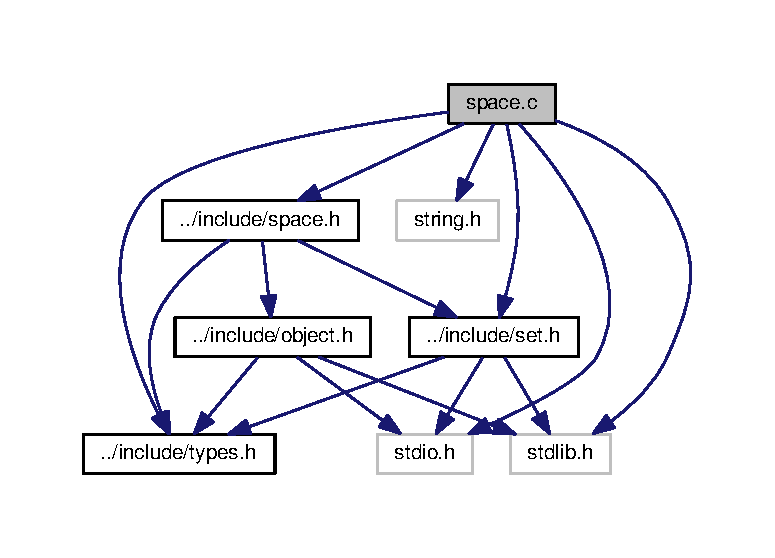
\includegraphics[width=350pt]{space_8c__incl}
\end{center}
\end{figure}
\subsection*{Classes}
\begin{DoxyCompactItemize}
\item 
struct \hyperlink{struct__Space}{\+\_\+\+Space}
\end{DoxyCompactItemize}
\subsection*{Functions}
\begin{DoxyCompactItemize}
\item 
\hyperlink{space_8h_a67533ffc2b70463baecc38fb0629bbfc}{Space} $\ast$ \hyperlink{space_8c_a162866fcea156b800fd546d0ffd271c9}{space\+\_\+create} (\hyperlink{types_8h_a845e604fb28f7e3d97549da3448149d3}{Id} id)
\item 
\hyperlink{types_8h_a32c27cc471df37f4fc818d65de0a56c4}{S\+T\+A\+T\+US} \hyperlink{space_8c_a5c70c70398923693ddbe4dfac8d72a0d}{space\+\_\+destroy} (\hyperlink{space_8h_a67533ffc2b70463baecc38fb0629bbfc}{Space} $\ast$space)
\item 
\hyperlink{types_8h_a32c27cc471df37f4fc818d65de0a56c4}{S\+T\+A\+T\+US} \hyperlink{space_8c_aab5b468f9822ab78dbe16d1321870d93}{space\+\_\+set\+\_\+name} (\hyperlink{space_8h_a67533ffc2b70463baecc38fb0629bbfc}{Space} $\ast$space, char $\ast$name)
\item 
\hyperlink{types_8h_a32c27cc471df37f4fc818d65de0a56c4}{S\+T\+A\+T\+US} \hyperlink{space_8c_a3d11ce59c10b61d9ea31a46e0ab6da13}{space\+\_\+set\+Sprite} (\hyperlink{space_8h_a67533ffc2b70463baecc38fb0629bbfc}{Space} $\ast$space, \hyperlink{types_8h_a845e604fb28f7e3d97549da3448149d3}{Id} sprite\+Id, int i)
\item 
\hyperlink{types_8h_a32c27cc471df37f4fc818d65de0a56c4}{S\+T\+A\+T\+US} \hyperlink{space_8c_a278d1f45c655e71ced22d208060e4baa}{space\+\_\+set\+Current\+Sprite} (\hyperlink{space_8h_a67533ffc2b70463baecc38fb0629bbfc}{Space} $\ast$space, int i)
\item 
\hyperlink{types_8h_a32c27cc471df37f4fc818d65de0a56c4}{S\+T\+A\+T\+US} \hyperlink{space_8c_a7aecc426029f567d452a0f916fd512d6}{space\+\_\+set\+\_\+description} (\hyperlink{space_8h_a67533ffc2b70463baecc38fb0629bbfc}{Space} $\ast$space, char $\ast$description)
\item 
\hyperlink{types_8h_a32c27cc471df37f4fc818d65de0a56c4}{S\+T\+A\+T\+US} \hyperlink{space_8c_a9e6e3e3bac4996ac6b8bd555e52bfb26}{space\+\_\+set\+\_\+north} (\hyperlink{space_8h_a67533ffc2b70463baecc38fb0629bbfc}{Space} $\ast$space, \hyperlink{types_8h_a845e604fb28f7e3d97549da3448149d3}{Id} id)
\item 
\hyperlink{types_8h_a32c27cc471df37f4fc818d65de0a56c4}{S\+T\+A\+T\+US} \hyperlink{space_8c_a422ab9f220b4c471c44256a27377de1a}{space\+\_\+set\+\_\+south} (\hyperlink{space_8h_a67533ffc2b70463baecc38fb0629bbfc}{Space} $\ast$space, \hyperlink{types_8h_a845e604fb28f7e3d97549da3448149d3}{Id} id)
\item 
\hyperlink{types_8h_a32c27cc471df37f4fc818d65de0a56c4}{S\+T\+A\+T\+US} \hyperlink{space_8c_a860a8f3e0227955ad56d1a12f0bdc44a}{space\+\_\+set\+\_\+east} (\hyperlink{space_8h_a67533ffc2b70463baecc38fb0629bbfc}{Space} $\ast$space, \hyperlink{types_8h_a845e604fb28f7e3d97549da3448149d3}{Id} id)
\item 
\hyperlink{types_8h_a32c27cc471df37f4fc818d65de0a56c4}{S\+T\+A\+T\+US} \hyperlink{space_8c_ad44b14cb38902cf31fa1f341beaab0db}{space\+\_\+set\+\_\+west} (\hyperlink{space_8h_a67533ffc2b70463baecc38fb0629bbfc}{Space} $\ast$space, \hyperlink{types_8h_a845e604fb28f7e3d97549da3448149d3}{Id} id)
\item 
\hyperlink{types_8h_a32c27cc471df37f4fc818d65de0a56c4}{S\+T\+A\+T\+US} \hyperlink{space_8c_aa2707bdca8fd356ed8d15fd48e820a4f}{space\+\_\+set\+\_\+up} (\hyperlink{space_8h_a67533ffc2b70463baecc38fb0629bbfc}{Space} $\ast$space, \hyperlink{types_8h_a845e604fb28f7e3d97549da3448149d3}{Id} id)
\item 
\hyperlink{types_8h_a32c27cc471df37f4fc818d65de0a56c4}{S\+T\+A\+T\+US} \hyperlink{space_8c_ae5b9fef52456ffccffbd73f882a56d23}{space\+\_\+set\+\_\+down} (\hyperlink{space_8h_a67533ffc2b70463baecc38fb0629bbfc}{Space} $\ast$space, \hyperlink{types_8h_a845e604fb28f7e3d97549da3448149d3}{Id} id)
\item 
\hyperlink{types_8h_a32c27cc471df37f4fc818d65de0a56c4}{S\+T\+A\+T\+US} \hyperlink{space_8c_a97cdd4deef92d7d220ed0fe70ebc68e2}{space\+\_\+set\+\_\+light} (\hyperlink{space_8h_a67533ffc2b70463baecc38fb0629bbfc}{Space} $\ast$space, \hyperlink{types_8h_a3e5b8192e7d9ffaf3542f1210aec18dd}{B\+O\+OL} light)
\item 
\hyperlink{types_8h_a3e5b8192e7d9ffaf3542f1210aec18dd}{B\+O\+OL} \hyperlink{space_8c_abae16fa836379f9fa4b22d9417b317b0}{space\+\_\+get\+\_\+light} (\hyperlink{space_8h_a67533ffc2b70463baecc38fb0629bbfc}{Space} $\ast$space)
\item 
\hyperlink{types_8h_a32c27cc471df37f4fc818d65de0a56c4}{S\+T\+A\+T\+US} \hyperlink{space_8c_a9116b7d1185d008776140782b03356cf}{space\+\_\+add\+\_\+object} (\hyperlink{space_8h_a67533ffc2b70463baecc38fb0629bbfc}{Space} $\ast$space, \hyperlink{types_8h_a845e604fb28f7e3d97549da3448149d3}{Id} obj\+\_\+id)
\item 
\hyperlink{types_8h_a32c27cc471df37f4fc818d65de0a56c4}{S\+T\+A\+T\+US} \hyperlink{space_8c_a4d8d68ad5dcf437ee8abd52ea30a268c}{space\+\_\+remove\+\_\+object} (\hyperlink{space_8h_a67533ffc2b70463baecc38fb0629bbfc}{Space} $\ast$space, \hyperlink{types_8h_a845e604fb28f7e3d97549da3448149d3}{Id} id)
\item 
\hyperlink{types_8h_a845e604fb28f7e3d97549da3448149d3}{Id} \hyperlink{space_8c_a56a13a586abce4825f49a490f09e6ec3}{space\+\_\+get\+Sprite} (\hyperlink{space_8h_a67533ffc2b70463baecc38fb0629bbfc}{Space} $\ast$space, int i)
\item 
int \hyperlink{space_8c_ab65e3bd927600c0af390d08817151013}{space\+\_\+get\+Curent\+Sprite} (\hyperlink{space_8h_a67533ffc2b70463baecc38fb0629bbfc}{Space} $\ast$space)
\item 
const char $\ast$ \hyperlink{space_8c_a310c540cd6e11073f7328add1f927001}{space\+\_\+get\+\_\+name} (\hyperlink{space_8h_a67533ffc2b70463baecc38fb0629bbfc}{Space} $\ast$space)
\item 
const char $\ast$ \hyperlink{space_8c_a51e854a2f9b35bd39e60c04ec5f03abd}{space\+\_\+get\+\_\+description} (\hyperlink{space_8h_a67533ffc2b70463baecc38fb0629bbfc}{Space} $\ast$space)
\item 
\hyperlink{types_8h_a845e604fb28f7e3d97549da3448149d3}{Id} \hyperlink{space_8c_ac8ddfd0d8692fd852ee49698c446cb50}{space\+\_\+get\+\_\+id} (\hyperlink{space_8h_a67533ffc2b70463baecc38fb0629bbfc}{Space} $\ast$space)
\item 
\hyperlink{types_8h_a845e604fb28f7e3d97549da3448149d3}{Id} \hyperlink{space_8c_ad331fba774897900f615d9d2e8d81a90}{space\+\_\+get\+\_\+north} (\hyperlink{space_8h_a67533ffc2b70463baecc38fb0629bbfc}{Space} $\ast$space)
\item 
\hyperlink{types_8h_a845e604fb28f7e3d97549da3448149d3}{Id} \hyperlink{space_8c_a9b86e1335c423eaad832e50d4c12cf1f}{space\+\_\+get\+\_\+south} (\hyperlink{space_8h_a67533ffc2b70463baecc38fb0629bbfc}{Space} $\ast$space)
\item 
\hyperlink{types_8h_a845e604fb28f7e3d97549da3448149d3}{Id} \hyperlink{space_8c_a978a22b77f74bb2dab68a00571abbe0b}{space\+\_\+get\+\_\+east} (\hyperlink{space_8h_a67533ffc2b70463baecc38fb0629bbfc}{Space} $\ast$space)
\item 
\hyperlink{types_8h_a845e604fb28f7e3d97549da3448149d3}{Id} \hyperlink{space_8c_af495ebfd5d13eba1a48cebd10992a17f}{space\+\_\+get\+\_\+west} (\hyperlink{space_8h_a67533ffc2b70463baecc38fb0629bbfc}{Space} $\ast$space)
\item 
\hyperlink{types_8h_a845e604fb28f7e3d97549da3448149d3}{Id} \hyperlink{space_8c_a174a988b899d5a0db889a31b70763c9c}{space\+\_\+get\+\_\+up} (\hyperlink{space_8h_a67533ffc2b70463baecc38fb0629bbfc}{Space} $\ast$space)
\item 
\hyperlink{types_8h_a845e604fb28f7e3d97549da3448149d3}{Id} \hyperlink{space_8c_ab269eab72b9ea7254044b34b1c177602}{space\+\_\+get\+\_\+down} (\hyperlink{space_8h_a67533ffc2b70463baecc38fb0629bbfc}{Space} $\ast$space)
\item 
\hyperlink{set_8h_a6d3b7f7c92cbb4577ef3ef7ddbf93161}{Set} $\ast$ \hyperlink{space_8c_ab100dcff5e360fb73b4e0a1f0e7505f7}{space\+\_\+get\+\_\+objects\+\_\+id} (\hyperlink{space_8h_a67533ffc2b70463baecc38fb0629bbfc}{Space} $\ast$space)
\item 
\hyperlink{types_8h_a32c27cc471df37f4fc818d65de0a56c4}{S\+T\+A\+T\+US} \hyperlink{space_8c_adbfe3a41783fc8b09735ba4e52a5bba8}{space\+\_\+light\+\_\+print} (\hyperlink{space_8h_a67533ffc2b70463baecc38fb0629bbfc}{Space} $\ast$space)
\item 
\hyperlink{types_8h_a32c27cc471df37f4fc818d65de0a56c4}{S\+T\+A\+T\+US} \hyperlink{space_8c_a18eca058da6cdf20ae5eda9d122d992e}{space\+\_\+print} (\hyperlink{space_8h_a67533ffc2b70463baecc38fb0629bbfc}{Space} $\ast$space)
\item 
\hyperlink{types_8h_a32c27cc471df37f4fc818d65de0a56c4}{S\+T\+A\+T\+US} \hyperlink{space_8c_a8eb9d9c2fc1804b555b3949fdf43c349}{space\+\_\+set\+\_\+gdesc\+\_\+0} (\hyperlink{space_8h_a67533ffc2b70463baecc38fb0629bbfc}{Space} $\ast$space, char $\ast$cadena)
\item 
\hyperlink{types_8h_a32c27cc471df37f4fc818d65de0a56c4}{S\+T\+A\+T\+US} \hyperlink{space_8c_a1e5de21b0c68de86effca65f9551b1f8}{space\+\_\+set\+\_\+gdesc\+\_\+1} (\hyperlink{space_8h_a67533ffc2b70463baecc38fb0629bbfc}{Space} $\ast$space, char $\ast$cadena)
\item 
\hyperlink{types_8h_a32c27cc471df37f4fc818d65de0a56c4}{S\+T\+A\+T\+US} \hyperlink{space_8c_ae1e1dde36d35428fe871f6b1b385e418}{space\+\_\+set\+\_\+gdesc\+\_\+2} (\hyperlink{space_8h_a67533ffc2b70463baecc38fb0629bbfc}{Space} $\ast$space, char $\ast$cadena)
\item 
char $\ast$ \hyperlink{space_8c_a3a41d5bdd686e58dd5c351eb15ca0cb2}{space\+\_\+get\+\_\+gdesc\+\_\+0} (\hyperlink{space_8h_a67533ffc2b70463baecc38fb0629bbfc}{Space} $\ast$space)
\item 
char $\ast$ \hyperlink{space_8c_a39c60f52b24bf33449887d97ed7e550b}{space\+\_\+get\+\_\+gdesc\+\_\+1} (\hyperlink{space_8h_a67533ffc2b70463baecc38fb0629bbfc}{Space} $\ast$space)
\item 
char $\ast$ \hyperlink{space_8c_a32db70300778094d5fd115822400d78e}{space\+\_\+get\+\_\+gdesc\+\_\+2} (\hyperlink{space_8h_a67533ffc2b70463baecc38fb0629bbfc}{Space} $\ast$space)
\end{DoxyCompactItemize}


\subsection{Function Documentation}
\index{space.\+c@{space.\+c}!space\+\_\+add\+\_\+object@{space\+\_\+add\+\_\+object}}
\index{space\+\_\+add\+\_\+object@{space\+\_\+add\+\_\+object}!space.\+c@{space.\+c}}
\subsubsection[{\texorpdfstring{space\+\_\+add\+\_\+object(\+Space $\ast$space, Id obj\+\_\+id)}{space_add_object(Space *space, Id obj_id)}}]{\setlength{\rightskip}{0pt plus 5cm}{\bf S\+T\+A\+T\+US} space\+\_\+add\+\_\+object (
\begin{DoxyParamCaption}
\item[{{\bf Space} $\ast$}]{space, }
\item[{{\bf Id}}]{obj\+\_\+id}
\end{DoxyParamCaption}
)}\hypertarget{space_8c_a9116b7d1185d008776140782b03356cf}{}\label{space_8c_a9116b7d1185d008776140782b03356cf}
\index{space.\+c@{space.\+c}!space\+\_\+create@{space\+\_\+create}}
\index{space\+\_\+create@{space\+\_\+create}!space.\+c@{space.\+c}}
\subsubsection[{\texorpdfstring{space\+\_\+create(\+Id id)}{space_create(Id id)}}]{\setlength{\rightskip}{0pt plus 5cm}{\bf Space}$\ast$ space\+\_\+create (
\begin{DoxyParamCaption}
\item[{{\bf Id}}]{id}
\end{DoxyParamCaption}
)}\hypertarget{space_8c_a162866fcea156b800fd546d0ffd271c9}{}\label{space_8c_a162866fcea156b800fd546d0ffd271c9}
\index{space.\+c@{space.\+c}!space\+\_\+destroy@{space\+\_\+destroy}}
\index{space\+\_\+destroy@{space\+\_\+destroy}!space.\+c@{space.\+c}}
\subsubsection[{\texorpdfstring{space\+\_\+destroy(\+Space $\ast$space)}{space_destroy(Space *space)}}]{\setlength{\rightskip}{0pt plus 5cm}{\bf S\+T\+A\+T\+US} space\+\_\+destroy (
\begin{DoxyParamCaption}
\item[{{\bf Space} $\ast$}]{space}
\end{DoxyParamCaption}
)}\hypertarget{space_8c_a5c70c70398923693ddbe4dfac8d72a0d}{}\label{space_8c_a5c70c70398923693ddbe4dfac8d72a0d}
\index{space.\+c@{space.\+c}!space\+\_\+get\+\_\+description@{space\+\_\+get\+\_\+description}}
\index{space\+\_\+get\+\_\+description@{space\+\_\+get\+\_\+description}!space.\+c@{space.\+c}}
\subsubsection[{\texorpdfstring{space\+\_\+get\+\_\+description(\+Space $\ast$space)}{space_get_description(Space *space)}}]{\setlength{\rightskip}{0pt plus 5cm}const char$\ast$ space\+\_\+get\+\_\+description (
\begin{DoxyParamCaption}
\item[{{\bf Space} $\ast$}]{space}
\end{DoxyParamCaption}
)}\hypertarget{space_8c_a51e854a2f9b35bd39e60c04ec5f03abd}{}\label{space_8c_a51e854a2f9b35bd39e60c04ec5f03abd}
\index{space.\+c@{space.\+c}!space\+\_\+get\+\_\+down@{space\+\_\+get\+\_\+down}}
\index{space\+\_\+get\+\_\+down@{space\+\_\+get\+\_\+down}!space.\+c@{space.\+c}}
\subsubsection[{\texorpdfstring{space\+\_\+get\+\_\+down(\+Space $\ast$space)}{space_get_down(Space *space)}}]{\setlength{\rightskip}{0pt plus 5cm}{\bf Id} space\+\_\+get\+\_\+down (
\begin{DoxyParamCaption}
\item[{{\bf Space} $\ast$}]{space}
\end{DoxyParamCaption}
)}\hypertarget{space_8c_ab269eab72b9ea7254044b34b1c177602}{}\label{space_8c_ab269eab72b9ea7254044b34b1c177602}
\index{space.\+c@{space.\+c}!space\+\_\+get\+\_\+east@{space\+\_\+get\+\_\+east}}
\index{space\+\_\+get\+\_\+east@{space\+\_\+get\+\_\+east}!space.\+c@{space.\+c}}
\subsubsection[{\texorpdfstring{space\+\_\+get\+\_\+east(\+Space $\ast$space)}{space_get_east(Space *space)}}]{\setlength{\rightskip}{0pt plus 5cm}{\bf Id} space\+\_\+get\+\_\+east (
\begin{DoxyParamCaption}
\item[{{\bf Space} $\ast$}]{space}
\end{DoxyParamCaption}
)}\hypertarget{space_8c_a978a22b77f74bb2dab68a00571abbe0b}{}\label{space_8c_a978a22b77f74bb2dab68a00571abbe0b}
\index{space.\+c@{space.\+c}!space\+\_\+get\+\_\+gdesc\+\_\+0@{space\+\_\+get\+\_\+gdesc\+\_\+0}}
\index{space\+\_\+get\+\_\+gdesc\+\_\+0@{space\+\_\+get\+\_\+gdesc\+\_\+0}!space.\+c@{space.\+c}}
\subsubsection[{\texorpdfstring{space\+\_\+get\+\_\+gdesc\+\_\+0(\+Space $\ast$space)}{space_get_gdesc_0(Space *space)}}]{\setlength{\rightskip}{0pt plus 5cm}char$\ast$ space\+\_\+get\+\_\+gdesc\+\_\+0 (
\begin{DoxyParamCaption}
\item[{{\bf Space} $\ast$}]{space}
\end{DoxyParamCaption}
)}\hypertarget{space_8c_a3a41d5bdd686e58dd5c351eb15ca0cb2}{}\label{space_8c_a3a41d5bdd686e58dd5c351eb15ca0cb2}
\index{space.\+c@{space.\+c}!space\+\_\+get\+\_\+gdesc\+\_\+1@{space\+\_\+get\+\_\+gdesc\+\_\+1}}
\index{space\+\_\+get\+\_\+gdesc\+\_\+1@{space\+\_\+get\+\_\+gdesc\+\_\+1}!space.\+c@{space.\+c}}
\subsubsection[{\texorpdfstring{space\+\_\+get\+\_\+gdesc\+\_\+1(\+Space $\ast$space)}{space_get_gdesc_1(Space *space)}}]{\setlength{\rightskip}{0pt plus 5cm}char$\ast$ space\+\_\+get\+\_\+gdesc\+\_\+1 (
\begin{DoxyParamCaption}
\item[{{\bf Space} $\ast$}]{space}
\end{DoxyParamCaption}
)}\hypertarget{space_8c_a39c60f52b24bf33449887d97ed7e550b}{}\label{space_8c_a39c60f52b24bf33449887d97ed7e550b}
\index{space.\+c@{space.\+c}!space\+\_\+get\+\_\+gdesc\+\_\+2@{space\+\_\+get\+\_\+gdesc\+\_\+2}}
\index{space\+\_\+get\+\_\+gdesc\+\_\+2@{space\+\_\+get\+\_\+gdesc\+\_\+2}!space.\+c@{space.\+c}}
\subsubsection[{\texorpdfstring{space\+\_\+get\+\_\+gdesc\+\_\+2(\+Space $\ast$space)}{space_get_gdesc_2(Space *space)}}]{\setlength{\rightskip}{0pt plus 5cm}char$\ast$ space\+\_\+get\+\_\+gdesc\+\_\+2 (
\begin{DoxyParamCaption}
\item[{{\bf Space} $\ast$}]{space}
\end{DoxyParamCaption}
)}\hypertarget{space_8c_a32db70300778094d5fd115822400d78e}{}\label{space_8c_a32db70300778094d5fd115822400d78e}
\index{space.\+c@{space.\+c}!space\+\_\+get\+\_\+id@{space\+\_\+get\+\_\+id}}
\index{space\+\_\+get\+\_\+id@{space\+\_\+get\+\_\+id}!space.\+c@{space.\+c}}
\subsubsection[{\texorpdfstring{space\+\_\+get\+\_\+id(\+Space $\ast$space)}{space_get_id(Space *space)}}]{\setlength{\rightskip}{0pt plus 5cm}{\bf Id} space\+\_\+get\+\_\+id (
\begin{DoxyParamCaption}
\item[{{\bf Space} $\ast$}]{space}
\end{DoxyParamCaption}
)}\hypertarget{space_8c_ac8ddfd0d8692fd852ee49698c446cb50}{}\label{space_8c_ac8ddfd0d8692fd852ee49698c446cb50}
\index{space.\+c@{space.\+c}!space\+\_\+get\+\_\+light@{space\+\_\+get\+\_\+light}}
\index{space\+\_\+get\+\_\+light@{space\+\_\+get\+\_\+light}!space.\+c@{space.\+c}}
\subsubsection[{\texorpdfstring{space\+\_\+get\+\_\+light(\+Space $\ast$space)}{space_get_light(Space *space)}}]{\setlength{\rightskip}{0pt plus 5cm}{\bf B\+O\+OL} space\+\_\+get\+\_\+light (
\begin{DoxyParamCaption}
\item[{{\bf Space} $\ast$}]{space}
\end{DoxyParamCaption}
)}\hypertarget{space_8c_abae16fa836379f9fa4b22d9417b317b0}{}\label{space_8c_abae16fa836379f9fa4b22d9417b317b0}
\index{space.\+c@{space.\+c}!space\+\_\+get\+\_\+name@{space\+\_\+get\+\_\+name}}
\index{space\+\_\+get\+\_\+name@{space\+\_\+get\+\_\+name}!space.\+c@{space.\+c}}
\subsubsection[{\texorpdfstring{space\+\_\+get\+\_\+name(\+Space $\ast$space)}{space_get_name(Space *space)}}]{\setlength{\rightskip}{0pt plus 5cm}const char$\ast$ space\+\_\+get\+\_\+name (
\begin{DoxyParamCaption}
\item[{{\bf Space} $\ast$}]{space}
\end{DoxyParamCaption}
)}\hypertarget{space_8c_a310c540cd6e11073f7328add1f927001}{}\label{space_8c_a310c540cd6e11073f7328add1f927001}
\index{space.\+c@{space.\+c}!space\+\_\+get\+\_\+north@{space\+\_\+get\+\_\+north}}
\index{space\+\_\+get\+\_\+north@{space\+\_\+get\+\_\+north}!space.\+c@{space.\+c}}
\subsubsection[{\texorpdfstring{space\+\_\+get\+\_\+north(\+Space $\ast$space)}{space_get_north(Space *space)}}]{\setlength{\rightskip}{0pt plus 5cm}{\bf Id} space\+\_\+get\+\_\+north (
\begin{DoxyParamCaption}
\item[{{\bf Space} $\ast$}]{space}
\end{DoxyParamCaption}
)}\hypertarget{space_8c_ad331fba774897900f615d9d2e8d81a90}{}\label{space_8c_ad331fba774897900f615d9d2e8d81a90}
\index{space.\+c@{space.\+c}!space\+\_\+get\+\_\+objects\+\_\+id@{space\+\_\+get\+\_\+objects\+\_\+id}}
\index{space\+\_\+get\+\_\+objects\+\_\+id@{space\+\_\+get\+\_\+objects\+\_\+id}!space.\+c@{space.\+c}}
\subsubsection[{\texorpdfstring{space\+\_\+get\+\_\+objects\+\_\+id(\+Space $\ast$space)}{space_get_objects_id(Space *space)}}]{\setlength{\rightskip}{0pt plus 5cm}{\bf Set}$\ast$ space\+\_\+get\+\_\+objects\+\_\+id (
\begin{DoxyParamCaption}
\item[{{\bf Space} $\ast$}]{space}
\end{DoxyParamCaption}
)}\hypertarget{space_8c_ab100dcff5e360fb73b4e0a1f0e7505f7}{}\label{space_8c_ab100dcff5e360fb73b4e0a1f0e7505f7}
\index{space.\+c@{space.\+c}!space\+\_\+get\+\_\+south@{space\+\_\+get\+\_\+south}}
\index{space\+\_\+get\+\_\+south@{space\+\_\+get\+\_\+south}!space.\+c@{space.\+c}}
\subsubsection[{\texorpdfstring{space\+\_\+get\+\_\+south(\+Space $\ast$space)}{space_get_south(Space *space)}}]{\setlength{\rightskip}{0pt plus 5cm}{\bf Id} space\+\_\+get\+\_\+south (
\begin{DoxyParamCaption}
\item[{{\bf Space} $\ast$}]{space}
\end{DoxyParamCaption}
)}\hypertarget{space_8c_a9b86e1335c423eaad832e50d4c12cf1f}{}\label{space_8c_a9b86e1335c423eaad832e50d4c12cf1f}
\index{space.\+c@{space.\+c}!space\+\_\+get\+\_\+up@{space\+\_\+get\+\_\+up}}
\index{space\+\_\+get\+\_\+up@{space\+\_\+get\+\_\+up}!space.\+c@{space.\+c}}
\subsubsection[{\texorpdfstring{space\+\_\+get\+\_\+up(\+Space $\ast$space)}{space_get_up(Space *space)}}]{\setlength{\rightskip}{0pt plus 5cm}{\bf Id} space\+\_\+get\+\_\+up (
\begin{DoxyParamCaption}
\item[{{\bf Space} $\ast$}]{space}
\end{DoxyParamCaption}
)}\hypertarget{space_8c_a174a988b899d5a0db889a31b70763c9c}{}\label{space_8c_a174a988b899d5a0db889a31b70763c9c}
\index{space.\+c@{space.\+c}!space\+\_\+get\+\_\+west@{space\+\_\+get\+\_\+west}}
\index{space\+\_\+get\+\_\+west@{space\+\_\+get\+\_\+west}!space.\+c@{space.\+c}}
\subsubsection[{\texorpdfstring{space\+\_\+get\+\_\+west(\+Space $\ast$space)}{space_get_west(Space *space)}}]{\setlength{\rightskip}{0pt plus 5cm}{\bf Id} space\+\_\+get\+\_\+west (
\begin{DoxyParamCaption}
\item[{{\bf Space} $\ast$}]{space}
\end{DoxyParamCaption}
)}\hypertarget{space_8c_af495ebfd5d13eba1a48cebd10992a17f}{}\label{space_8c_af495ebfd5d13eba1a48cebd10992a17f}
\index{space.\+c@{space.\+c}!space\+\_\+get\+Curent\+Sprite@{space\+\_\+get\+Curent\+Sprite}}
\index{space\+\_\+get\+Curent\+Sprite@{space\+\_\+get\+Curent\+Sprite}!space.\+c@{space.\+c}}
\subsubsection[{\texorpdfstring{space\+\_\+get\+Curent\+Sprite(\+Space $\ast$space)}{space_getCurentSprite(Space *space)}}]{\setlength{\rightskip}{0pt plus 5cm}int space\+\_\+get\+Curent\+Sprite (
\begin{DoxyParamCaption}
\item[{{\bf Space} $\ast$}]{space}
\end{DoxyParamCaption}
)}\hypertarget{space_8c_ab65e3bd927600c0af390d08817151013}{}\label{space_8c_ab65e3bd927600c0af390d08817151013}
\index{space.\+c@{space.\+c}!space\+\_\+get\+Sprite@{space\+\_\+get\+Sprite}}
\index{space\+\_\+get\+Sprite@{space\+\_\+get\+Sprite}!space.\+c@{space.\+c}}
\subsubsection[{\texorpdfstring{space\+\_\+get\+Sprite(\+Space $\ast$space, int i)}{space_getSprite(Space *space, int i)}}]{\setlength{\rightskip}{0pt plus 5cm}{\bf Id} space\+\_\+get\+Sprite (
\begin{DoxyParamCaption}
\item[{{\bf Space} $\ast$}]{space, }
\item[{int}]{i}
\end{DoxyParamCaption}
)}\hypertarget{space_8c_a56a13a586abce4825f49a490f09e6ec3}{}\label{space_8c_a56a13a586abce4825f49a490f09e6ec3}
\index{space.\+c@{space.\+c}!space\+\_\+light\+\_\+print@{space\+\_\+light\+\_\+print}}
\index{space\+\_\+light\+\_\+print@{space\+\_\+light\+\_\+print}!space.\+c@{space.\+c}}
\subsubsection[{\texorpdfstring{space\+\_\+light\+\_\+print(\+Space $\ast$space)}{space_light_print(Space *space)}}]{\setlength{\rightskip}{0pt plus 5cm}{\bf S\+T\+A\+T\+US} space\+\_\+light\+\_\+print (
\begin{DoxyParamCaption}
\item[{{\bf Space} $\ast$}]{space}
\end{DoxyParamCaption}
)}\hypertarget{space_8c_adbfe3a41783fc8b09735ba4e52a5bba8}{}\label{space_8c_adbfe3a41783fc8b09735ba4e52a5bba8}
\index{space.\+c@{space.\+c}!space\+\_\+print@{space\+\_\+print}}
\index{space\+\_\+print@{space\+\_\+print}!space.\+c@{space.\+c}}
\subsubsection[{\texorpdfstring{space\+\_\+print(\+Space $\ast$space)}{space_print(Space *space)}}]{\setlength{\rightskip}{0pt plus 5cm}{\bf S\+T\+A\+T\+US} space\+\_\+print (
\begin{DoxyParamCaption}
\item[{{\bf Space} $\ast$}]{space}
\end{DoxyParamCaption}
)}\hypertarget{space_8c_a18eca058da6cdf20ae5eda9d122d992e}{}\label{space_8c_a18eca058da6cdf20ae5eda9d122d992e}
\index{space.\+c@{space.\+c}!space\+\_\+remove\+\_\+object@{space\+\_\+remove\+\_\+object}}
\index{space\+\_\+remove\+\_\+object@{space\+\_\+remove\+\_\+object}!space.\+c@{space.\+c}}
\subsubsection[{\texorpdfstring{space\+\_\+remove\+\_\+object(\+Space $\ast$space, Id id)}{space_remove_object(Space *space, Id id)}}]{\setlength{\rightskip}{0pt plus 5cm}{\bf S\+T\+A\+T\+US} space\+\_\+remove\+\_\+object (
\begin{DoxyParamCaption}
\item[{{\bf Space} $\ast$}]{space, }
\item[{{\bf Id}}]{id}
\end{DoxyParamCaption}
)}\hypertarget{space_8c_a4d8d68ad5dcf437ee8abd52ea30a268c}{}\label{space_8c_a4d8d68ad5dcf437ee8abd52ea30a268c}
\index{space.\+c@{space.\+c}!space\+\_\+set\+\_\+description@{space\+\_\+set\+\_\+description}}
\index{space\+\_\+set\+\_\+description@{space\+\_\+set\+\_\+description}!space.\+c@{space.\+c}}
\subsubsection[{\texorpdfstring{space\+\_\+set\+\_\+description(\+Space $\ast$space, char $\ast$description)}{space_set_description(Space *space, char *description)}}]{\setlength{\rightskip}{0pt plus 5cm}{\bf S\+T\+A\+T\+US} space\+\_\+set\+\_\+description (
\begin{DoxyParamCaption}
\item[{{\bf Space} $\ast$}]{space, }
\item[{char $\ast$}]{description}
\end{DoxyParamCaption}
)}\hypertarget{space_8c_a7aecc426029f567d452a0f916fd512d6}{}\label{space_8c_a7aecc426029f567d452a0f916fd512d6}
\index{space.\+c@{space.\+c}!space\+\_\+set\+\_\+down@{space\+\_\+set\+\_\+down}}
\index{space\+\_\+set\+\_\+down@{space\+\_\+set\+\_\+down}!space.\+c@{space.\+c}}
\subsubsection[{\texorpdfstring{space\+\_\+set\+\_\+down(\+Space $\ast$space, Id id)}{space_set_down(Space *space, Id id)}}]{\setlength{\rightskip}{0pt plus 5cm}{\bf S\+T\+A\+T\+US} space\+\_\+set\+\_\+down (
\begin{DoxyParamCaption}
\item[{{\bf Space} $\ast$}]{space, }
\item[{{\bf Id}}]{id}
\end{DoxyParamCaption}
)}\hypertarget{space_8c_ae5b9fef52456ffccffbd73f882a56d23}{}\label{space_8c_ae5b9fef52456ffccffbd73f882a56d23}
\index{space.\+c@{space.\+c}!space\+\_\+set\+\_\+east@{space\+\_\+set\+\_\+east}}
\index{space\+\_\+set\+\_\+east@{space\+\_\+set\+\_\+east}!space.\+c@{space.\+c}}
\subsubsection[{\texorpdfstring{space\+\_\+set\+\_\+east(\+Space $\ast$space, Id id)}{space_set_east(Space *space, Id id)}}]{\setlength{\rightskip}{0pt plus 5cm}{\bf S\+T\+A\+T\+US} space\+\_\+set\+\_\+east (
\begin{DoxyParamCaption}
\item[{{\bf Space} $\ast$}]{space, }
\item[{{\bf Id}}]{id}
\end{DoxyParamCaption}
)}\hypertarget{space_8c_a860a8f3e0227955ad56d1a12f0bdc44a}{}\label{space_8c_a860a8f3e0227955ad56d1a12f0bdc44a}
\index{space.\+c@{space.\+c}!space\+\_\+set\+\_\+gdesc\+\_\+0@{space\+\_\+set\+\_\+gdesc\+\_\+0}}
\index{space\+\_\+set\+\_\+gdesc\+\_\+0@{space\+\_\+set\+\_\+gdesc\+\_\+0}!space.\+c@{space.\+c}}
\subsubsection[{\texorpdfstring{space\+\_\+set\+\_\+gdesc\+\_\+0(\+Space $\ast$space, char $\ast$cadena)}{space_set_gdesc_0(Space *space, char *cadena)}}]{\setlength{\rightskip}{0pt plus 5cm}{\bf S\+T\+A\+T\+US} space\+\_\+set\+\_\+gdesc\+\_\+0 (
\begin{DoxyParamCaption}
\item[{{\bf Space} $\ast$}]{space, }
\item[{char $\ast$}]{cadena}
\end{DoxyParamCaption}
)}\hypertarget{space_8c_a8eb9d9c2fc1804b555b3949fdf43c349}{}\label{space_8c_a8eb9d9c2fc1804b555b3949fdf43c349}
\index{space.\+c@{space.\+c}!space\+\_\+set\+\_\+gdesc\+\_\+1@{space\+\_\+set\+\_\+gdesc\+\_\+1}}
\index{space\+\_\+set\+\_\+gdesc\+\_\+1@{space\+\_\+set\+\_\+gdesc\+\_\+1}!space.\+c@{space.\+c}}
\subsubsection[{\texorpdfstring{space\+\_\+set\+\_\+gdesc\+\_\+1(\+Space $\ast$space, char $\ast$cadena)}{space_set_gdesc_1(Space *space, char *cadena)}}]{\setlength{\rightskip}{0pt plus 5cm}{\bf S\+T\+A\+T\+US} space\+\_\+set\+\_\+gdesc\+\_\+1 (
\begin{DoxyParamCaption}
\item[{{\bf Space} $\ast$}]{space, }
\item[{char $\ast$}]{cadena}
\end{DoxyParamCaption}
)}\hypertarget{space_8c_a1e5de21b0c68de86effca65f9551b1f8}{}\label{space_8c_a1e5de21b0c68de86effca65f9551b1f8}
\index{space.\+c@{space.\+c}!space\+\_\+set\+\_\+gdesc\+\_\+2@{space\+\_\+set\+\_\+gdesc\+\_\+2}}
\index{space\+\_\+set\+\_\+gdesc\+\_\+2@{space\+\_\+set\+\_\+gdesc\+\_\+2}!space.\+c@{space.\+c}}
\subsubsection[{\texorpdfstring{space\+\_\+set\+\_\+gdesc\+\_\+2(\+Space $\ast$space, char $\ast$cadena)}{space_set_gdesc_2(Space *space, char *cadena)}}]{\setlength{\rightskip}{0pt plus 5cm}{\bf S\+T\+A\+T\+US} space\+\_\+set\+\_\+gdesc\+\_\+2 (
\begin{DoxyParamCaption}
\item[{{\bf Space} $\ast$}]{space, }
\item[{char $\ast$}]{cadena}
\end{DoxyParamCaption}
)}\hypertarget{space_8c_ae1e1dde36d35428fe871f6b1b385e418}{}\label{space_8c_ae1e1dde36d35428fe871f6b1b385e418}
\index{space.\+c@{space.\+c}!space\+\_\+set\+\_\+light@{space\+\_\+set\+\_\+light}}
\index{space\+\_\+set\+\_\+light@{space\+\_\+set\+\_\+light}!space.\+c@{space.\+c}}
\subsubsection[{\texorpdfstring{space\+\_\+set\+\_\+light(\+Space $\ast$space, B\+O\+O\+L light)}{space_set_light(Space *space, BOOL light)}}]{\setlength{\rightskip}{0pt plus 5cm}{\bf S\+T\+A\+T\+US} space\+\_\+set\+\_\+light (
\begin{DoxyParamCaption}
\item[{{\bf Space} $\ast$}]{space, }
\item[{{\bf B\+O\+OL}}]{light}
\end{DoxyParamCaption}
)}\hypertarget{space_8c_a97cdd4deef92d7d220ed0fe70ebc68e2}{}\label{space_8c_a97cdd4deef92d7d220ed0fe70ebc68e2}
\index{space.\+c@{space.\+c}!space\+\_\+set\+\_\+name@{space\+\_\+set\+\_\+name}}
\index{space\+\_\+set\+\_\+name@{space\+\_\+set\+\_\+name}!space.\+c@{space.\+c}}
\subsubsection[{\texorpdfstring{space\+\_\+set\+\_\+name(\+Space $\ast$space, char $\ast$name)}{space_set_name(Space *space, char *name)}}]{\setlength{\rightskip}{0pt plus 5cm}{\bf S\+T\+A\+T\+US} space\+\_\+set\+\_\+name (
\begin{DoxyParamCaption}
\item[{{\bf Space} $\ast$}]{space, }
\item[{char $\ast$}]{name}
\end{DoxyParamCaption}
)}\hypertarget{space_8c_aab5b468f9822ab78dbe16d1321870d93}{}\label{space_8c_aab5b468f9822ab78dbe16d1321870d93}
\index{space.\+c@{space.\+c}!space\+\_\+set\+\_\+north@{space\+\_\+set\+\_\+north}}
\index{space\+\_\+set\+\_\+north@{space\+\_\+set\+\_\+north}!space.\+c@{space.\+c}}
\subsubsection[{\texorpdfstring{space\+\_\+set\+\_\+north(\+Space $\ast$space, Id id)}{space_set_north(Space *space, Id id)}}]{\setlength{\rightskip}{0pt plus 5cm}{\bf S\+T\+A\+T\+US} space\+\_\+set\+\_\+north (
\begin{DoxyParamCaption}
\item[{{\bf Space} $\ast$}]{space, }
\item[{{\bf Id}}]{id}
\end{DoxyParamCaption}
)}\hypertarget{space_8c_a9e6e3e3bac4996ac6b8bd555e52bfb26}{}\label{space_8c_a9e6e3e3bac4996ac6b8bd555e52bfb26}
\index{space.\+c@{space.\+c}!space\+\_\+set\+\_\+south@{space\+\_\+set\+\_\+south}}
\index{space\+\_\+set\+\_\+south@{space\+\_\+set\+\_\+south}!space.\+c@{space.\+c}}
\subsubsection[{\texorpdfstring{space\+\_\+set\+\_\+south(\+Space $\ast$space, Id id)}{space_set_south(Space *space, Id id)}}]{\setlength{\rightskip}{0pt plus 5cm}{\bf S\+T\+A\+T\+US} space\+\_\+set\+\_\+south (
\begin{DoxyParamCaption}
\item[{{\bf Space} $\ast$}]{space, }
\item[{{\bf Id}}]{id}
\end{DoxyParamCaption}
)}\hypertarget{space_8c_a422ab9f220b4c471c44256a27377de1a}{}\label{space_8c_a422ab9f220b4c471c44256a27377de1a}
\index{space.\+c@{space.\+c}!space\+\_\+set\+\_\+up@{space\+\_\+set\+\_\+up}}
\index{space\+\_\+set\+\_\+up@{space\+\_\+set\+\_\+up}!space.\+c@{space.\+c}}
\subsubsection[{\texorpdfstring{space\+\_\+set\+\_\+up(\+Space $\ast$space, Id id)}{space_set_up(Space *space, Id id)}}]{\setlength{\rightskip}{0pt plus 5cm}{\bf S\+T\+A\+T\+US} space\+\_\+set\+\_\+up (
\begin{DoxyParamCaption}
\item[{{\bf Space} $\ast$}]{space, }
\item[{{\bf Id}}]{id}
\end{DoxyParamCaption}
)}\hypertarget{space_8c_aa2707bdca8fd356ed8d15fd48e820a4f}{}\label{space_8c_aa2707bdca8fd356ed8d15fd48e820a4f}
\index{space.\+c@{space.\+c}!space\+\_\+set\+\_\+west@{space\+\_\+set\+\_\+west}}
\index{space\+\_\+set\+\_\+west@{space\+\_\+set\+\_\+west}!space.\+c@{space.\+c}}
\subsubsection[{\texorpdfstring{space\+\_\+set\+\_\+west(\+Space $\ast$space, Id id)}{space_set_west(Space *space, Id id)}}]{\setlength{\rightskip}{0pt plus 5cm}{\bf S\+T\+A\+T\+US} space\+\_\+set\+\_\+west (
\begin{DoxyParamCaption}
\item[{{\bf Space} $\ast$}]{space, }
\item[{{\bf Id}}]{id}
\end{DoxyParamCaption}
)}\hypertarget{space_8c_ad44b14cb38902cf31fa1f341beaab0db}{}\label{space_8c_ad44b14cb38902cf31fa1f341beaab0db}
\index{space.\+c@{space.\+c}!space\+\_\+set\+Current\+Sprite@{space\+\_\+set\+Current\+Sprite}}
\index{space\+\_\+set\+Current\+Sprite@{space\+\_\+set\+Current\+Sprite}!space.\+c@{space.\+c}}
\subsubsection[{\texorpdfstring{space\+\_\+set\+Current\+Sprite(\+Space $\ast$space, int i)}{space_setCurrentSprite(Space *space, int i)}}]{\setlength{\rightskip}{0pt plus 5cm}{\bf S\+T\+A\+T\+US} space\+\_\+set\+Current\+Sprite (
\begin{DoxyParamCaption}
\item[{{\bf Space} $\ast$}]{space, }
\item[{int}]{i}
\end{DoxyParamCaption}
)}\hypertarget{space_8c_a278d1f45c655e71ced22d208060e4baa}{}\label{space_8c_a278d1f45c655e71ced22d208060e4baa}
\index{space.\+c@{space.\+c}!space\+\_\+set\+Sprite@{space\+\_\+set\+Sprite}}
\index{space\+\_\+set\+Sprite@{space\+\_\+set\+Sprite}!space.\+c@{space.\+c}}
\subsubsection[{\texorpdfstring{space\+\_\+set\+Sprite(\+Space $\ast$space, Id sprite\+Id, int i)}{space_setSprite(Space *space, Id spriteId, int i)}}]{\setlength{\rightskip}{0pt plus 5cm}{\bf S\+T\+A\+T\+US} space\+\_\+set\+Sprite (
\begin{DoxyParamCaption}
\item[{{\bf Space} $\ast$}]{space, }
\item[{{\bf Id}}]{sprite\+Id, }
\item[{int}]{i}
\end{DoxyParamCaption}
)}\hypertarget{space_8c_a3d11ce59c10b61d9ea31a46e0ab6da13}{}\label{space_8c_a3d11ce59c10b61d9ea31a46e0ab6da13}

\hypertarget{space_8h}{\section{space.\+h File Reference}
\label{space_8h}\index{space.\+h@{space.\+h}}
}


Defines functions for space manipulation.  


{\ttfamily \#include \char`\"{}../include/types.\+h\char`\"{}}\\*
{\ttfamily \#include \char`\"{}../include/object.\+h\char`\"{}}\\*
{\ttfamily \#include \char`\"{}../include/set.\+h\char`\"{}}\\*
Include dependency graph for space.\+h\+:\nopagebreak
\begin{figure}[H]
\begin{center}
\leavevmode
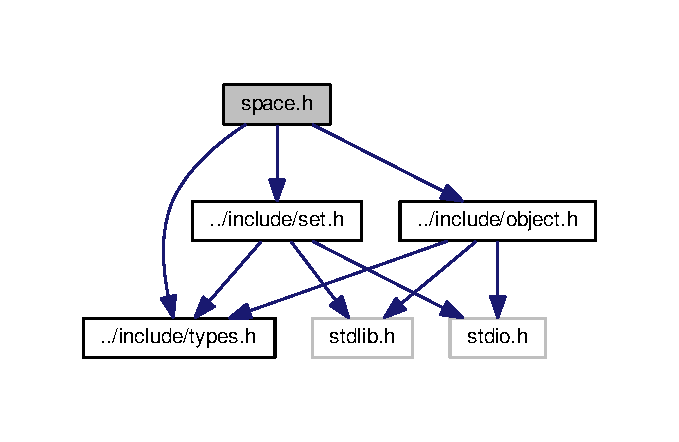
\includegraphics[width=326pt]{space_8h__incl}
\end{center}
\end{figure}
This graph shows which files directly or indirectly include this file\+:\nopagebreak
\begin{figure}[H]
\begin{center}
\leavevmode
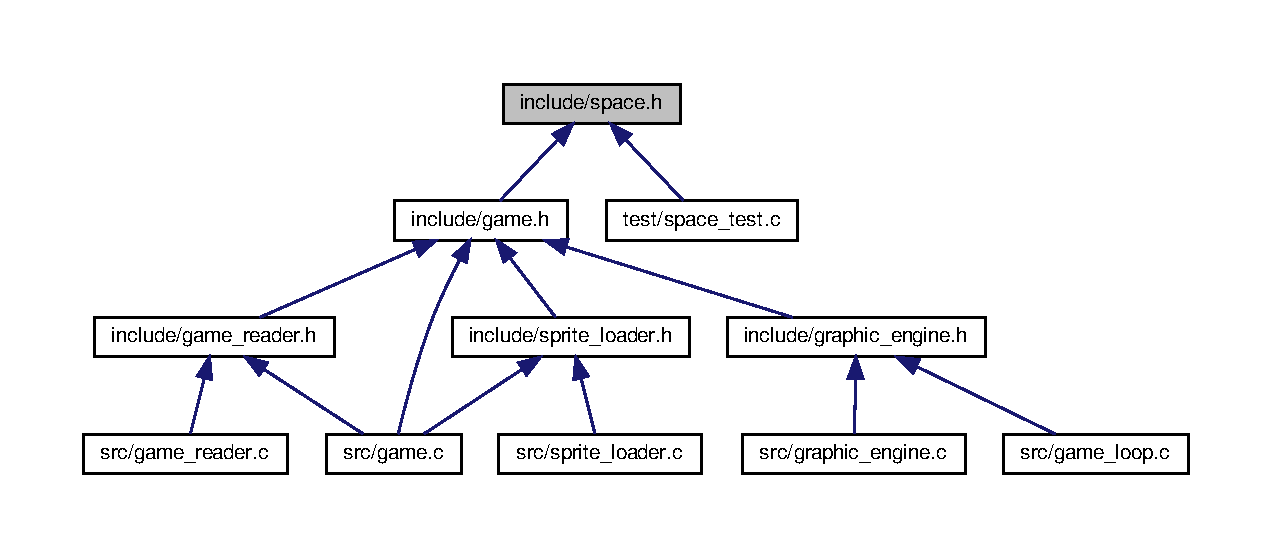
\includegraphics[width=350pt]{space_8h__dep__incl}
\end{center}
\end{figure}
\subsection*{Macros}
\begin{DoxyCompactItemize}
\item 
\#define \hyperlink{space_8h_a5f54fd55f983a2e33ce076cd9f587e82}{M\+A\+X\+\_\+\+S\+P\+A\+C\+E\+S}~100
\item 
\#define \hyperlink{space_8h_a088cbe7c6f78264d46c2624194c5c680}{F\+I\+R\+S\+T\+\_\+\+S\+P\+A\+C\+E}~1
\end{DoxyCompactItemize}
\subsection*{Typedefs}
\begin{DoxyCompactItemize}
\item 
typedef struct \hyperlink{struct__Space}{\+\_\+\+Space} \hyperlink{space_8h_a67533ffc2b70463baecc38fb0629bbfc}{Space}
\end{DoxyCompactItemize}
\subsection*{Functions}
\begin{DoxyCompactItemize}
\item 
\hyperlink{space_8h_a67533ffc2b70463baecc38fb0629bbfc}{Space} $\ast$ \hyperlink{space_8h_a162866fcea156b800fd546d0ffd271c9}{space\+\_\+create} (\hyperlink{types_8h_a845e604fb28f7e3d97549da3448149d3}{Id} id)
\item 
\hyperlink{types_8h_a32c27cc471df37f4fc818d65de0a56c4}{S\+T\+A\+T\+U\+S} \hyperlink{space_8h_a5c70c70398923693ddbe4dfac8d72a0d}{space\+\_\+destroy} (\hyperlink{space_8h_a67533ffc2b70463baecc38fb0629bbfc}{Space} $\ast$space)
\item 
\hyperlink{types_8h_a845e604fb28f7e3d97549da3448149d3}{Id} \hyperlink{space_8h_ac8ddfd0d8692fd852ee49698c446cb50}{space\+\_\+get\+\_\+id} (\hyperlink{space_8h_a67533ffc2b70463baecc38fb0629bbfc}{Space} $\ast$space)
\item 
\hyperlink{types_8h_a32c27cc471df37f4fc818d65de0a56c4}{S\+T\+A\+T\+U\+S} \hyperlink{space_8h_aab5b468f9822ab78dbe16d1321870d93}{space\+\_\+set\+\_\+name} (\hyperlink{space_8h_a67533ffc2b70463baecc38fb0629bbfc}{Space} $\ast$space, char $\ast$name)
\item 
const char $\ast$ \hyperlink{space_8h_a310c540cd6e11073f7328add1f927001}{space\+\_\+get\+\_\+name} (\hyperlink{space_8h_a67533ffc2b70463baecc38fb0629bbfc}{Space} $\ast$space)
\item 
\hyperlink{types_8h_a32c27cc471df37f4fc818d65de0a56c4}{S\+T\+A\+T\+U\+S} \hyperlink{space_8h_a7aecc426029f567d452a0f916fd512d6}{space\+\_\+set\+\_\+description} (\hyperlink{space_8h_a67533ffc2b70463baecc38fb0629bbfc}{Space} $\ast$space, char $\ast$description)
\item 
const char $\ast$ \hyperlink{space_8h_a51e854a2f9b35bd39e60c04ec5f03abd}{space\+\_\+get\+\_\+description} (\hyperlink{space_8h_a67533ffc2b70463baecc38fb0629bbfc}{Space} $\ast$space)
\item 
\hyperlink{types_8h_a32c27cc471df37f4fc818d65de0a56c4}{S\+T\+A\+T\+U\+S} \hyperlink{space_8h_a9e6e3e3bac4996ac6b8bd555e52bfb26}{space\+\_\+set\+\_\+north} (\hyperlink{space_8h_a67533ffc2b70463baecc38fb0629bbfc}{Space} $\ast$space, \hyperlink{types_8h_a845e604fb28f7e3d97549da3448149d3}{Id} id)
\item 
\hyperlink{types_8h_a845e604fb28f7e3d97549da3448149d3}{Id} \hyperlink{space_8h_ad331fba774897900f615d9d2e8d81a90}{space\+\_\+get\+\_\+north} (\hyperlink{space_8h_a67533ffc2b70463baecc38fb0629bbfc}{Space} $\ast$space)
\item 
\hyperlink{types_8h_a32c27cc471df37f4fc818d65de0a56c4}{S\+T\+A\+T\+U\+S} \hyperlink{space_8h_a422ab9f220b4c471c44256a27377de1a}{space\+\_\+set\+\_\+south} (\hyperlink{space_8h_a67533ffc2b70463baecc38fb0629bbfc}{Space} $\ast$space, \hyperlink{types_8h_a845e604fb28f7e3d97549da3448149d3}{Id} id)
\item 
\hyperlink{types_8h_a845e604fb28f7e3d97549da3448149d3}{Id} \hyperlink{space_8h_a9b86e1335c423eaad832e50d4c12cf1f}{space\+\_\+get\+\_\+south} (\hyperlink{space_8h_a67533ffc2b70463baecc38fb0629bbfc}{Space} $\ast$space)
\item 
\hyperlink{types_8h_a32c27cc471df37f4fc818d65de0a56c4}{S\+T\+A\+T\+U\+S} \hyperlink{space_8h_a860a8f3e0227955ad56d1a12f0bdc44a}{space\+\_\+set\+\_\+east} (\hyperlink{space_8h_a67533ffc2b70463baecc38fb0629bbfc}{Space} $\ast$space, \hyperlink{types_8h_a845e604fb28f7e3d97549da3448149d3}{Id} id)
\item 
\hyperlink{types_8h_a845e604fb28f7e3d97549da3448149d3}{Id} \hyperlink{space_8h_a978a22b77f74bb2dab68a00571abbe0b}{space\+\_\+get\+\_\+east} (\hyperlink{space_8h_a67533ffc2b70463baecc38fb0629bbfc}{Space} $\ast$space)
\item 
\hyperlink{types_8h_a32c27cc471df37f4fc818d65de0a56c4}{S\+T\+A\+T\+U\+S} \hyperlink{space_8h_ad44b14cb38902cf31fa1f341beaab0db}{space\+\_\+set\+\_\+west} (\hyperlink{space_8h_a67533ffc2b70463baecc38fb0629bbfc}{Space} $\ast$space, \hyperlink{types_8h_a845e604fb28f7e3d97549da3448149d3}{Id} id)
\item 
\hyperlink{types_8h_a845e604fb28f7e3d97549da3448149d3}{Id} \hyperlink{space_8h_af495ebfd5d13eba1a48cebd10992a17f}{space\+\_\+get\+\_\+west} (\hyperlink{space_8h_a67533ffc2b70463baecc38fb0629bbfc}{Space} $\ast$space)
\item 
\hyperlink{types_8h_a32c27cc471df37f4fc818d65de0a56c4}{S\+T\+A\+T\+U\+S} \hyperlink{space_8h_a9116b7d1185d008776140782b03356cf}{space\+\_\+add\+\_\+object} (\hyperlink{space_8h_a67533ffc2b70463baecc38fb0629bbfc}{Space} $\ast$space, \hyperlink{types_8h_a845e604fb28f7e3d97549da3448149d3}{Id} obj\+\_\+id)
\item 
\hyperlink{types_8h_a32c27cc471df37f4fc818d65de0a56c4}{S\+T\+A\+T\+U\+S} \hyperlink{space_8h_ab9adb4c54a074f40fba5c342b8645fe7}{space\+\_\+remove\+\_\+object} (\hyperlink{space_8h_a67533ffc2b70463baecc38fb0629bbfc}{Space} $\ast$space, \hyperlink{types_8h_a845e604fb28f7e3d97549da3448149d3}{Id} obj\+\_\+id)
\item 
\hyperlink{set_8h_a6d3b7f7c92cbb4577ef3ef7ddbf93161}{Set} $\ast$ \hyperlink{space_8h_ab100dcff5e360fb73b4e0a1f0e7505f7}{space\+\_\+get\+\_\+objects\+\_\+id} (\hyperlink{space_8h_a67533ffc2b70463baecc38fb0629bbfc}{Space} $\ast$space)
\item 
\hyperlink{types_8h_a32c27cc471df37f4fc818d65de0a56c4}{S\+T\+A\+T\+U\+S} \hyperlink{space_8h_a156c31e7022babf144e76a2266ab55f7}{space\+\_\+set\+\_\+gdesc\+\_\+0} (\hyperlink{space_8h_a67533ffc2b70463baecc38fb0629bbfc}{Space} $\ast$, char $\ast$)
\item 
\hyperlink{types_8h_a32c27cc471df37f4fc818d65de0a56c4}{S\+T\+A\+T\+U\+S} \hyperlink{space_8h_aaa00d9d57baac83fd7864c02c595ad00}{space\+\_\+set\+\_\+gdesc\+\_\+1} (\hyperlink{space_8h_a67533ffc2b70463baecc38fb0629bbfc}{Space} $\ast$, char $\ast$)
\item 
\hyperlink{types_8h_a32c27cc471df37f4fc818d65de0a56c4}{S\+T\+A\+T\+U\+S} \hyperlink{space_8h_ae0c43e47b9d7bf9254d5b10caacfc384}{space\+\_\+set\+\_\+gdesc\+\_\+2} (\hyperlink{space_8h_a67533ffc2b70463baecc38fb0629bbfc}{Space} $\ast$, char $\ast$)
\item 
char $\ast$ \hyperlink{space_8h_a79d5fdbe1a4e8cf5ce0f44d1e0495025}{space\+\_\+get\+\_\+gdesc\+\_\+0} (\hyperlink{space_8h_a67533ffc2b70463baecc38fb0629bbfc}{Space} $\ast$)
\item 
char $\ast$ \hyperlink{space_8h_a22693310bda91ac4cfaddb78fc781dde}{space\+\_\+get\+\_\+gdesc\+\_\+1} (\hyperlink{space_8h_a67533ffc2b70463baecc38fb0629bbfc}{Space} $\ast$)
\item 
char $\ast$ \hyperlink{space_8h_a74b9de467700f498bfbddacfa1119657}{space\+\_\+get\+\_\+gdesc\+\_\+2} (\hyperlink{space_8h_a67533ffc2b70463baecc38fb0629bbfc}{Space} $\ast$)
\item 
\hyperlink{types_8h_a32c27cc471df37f4fc818d65de0a56c4}{S\+T\+A\+T\+U\+S} \hyperlink{space_8h_a18eca058da6cdf20ae5eda9d122d992e}{space\+\_\+print} (\hyperlink{space_8h_a67533ffc2b70463baecc38fb0629bbfc}{Space} $\ast$space)
\end{DoxyCompactItemize}


\subsection{Detailed Description}
Defines functions for space manipulation. 

\begin{DoxyAuthor}{Author}
Catalín Rotaru 
\end{DoxyAuthor}
\begin{DoxyCopyright}{Copyright}
G\+N\+U Public License 
\end{DoxyCopyright}


\subsection{Macro Definition Documentation}
\hypertarget{space_8h_a088cbe7c6f78264d46c2624194c5c680}{\index{space.\+h@{space.\+h}!F\+I\+R\+S\+T\+\_\+\+S\+P\+A\+C\+E@{F\+I\+R\+S\+T\+\_\+\+S\+P\+A\+C\+E}}
\index{F\+I\+R\+S\+T\+\_\+\+S\+P\+A\+C\+E@{F\+I\+R\+S\+T\+\_\+\+S\+P\+A\+C\+E}!space.\+h@{space.\+h}}
\subsubsection[{F\+I\+R\+S\+T\+\_\+\+S\+P\+A\+C\+E}]{\setlength{\rightskip}{0pt plus 5cm}\#define F\+I\+R\+S\+T\+\_\+\+S\+P\+A\+C\+E~1}}\label{space_8h_a088cbe7c6f78264d46c2624194c5c680}
\hypertarget{space_8h_a5f54fd55f983a2e33ce076cd9f587e82}{\index{space.\+h@{space.\+h}!M\+A\+X\+\_\+\+S\+P\+A\+C\+E\+S@{M\+A\+X\+\_\+\+S\+P\+A\+C\+E\+S}}
\index{M\+A\+X\+\_\+\+S\+P\+A\+C\+E\+S@{M\+A\+X\+\_\+\+S\+P\+A\+C\+E\+S}!space.\+h@{space.\+h}}
\subsubsection[{M\+A\+X\+\_\+\+S\+P\+A\+C\+E\+S}]{\setlength{\rightskip}{0pt plus 5cm}\#define M\+A\+X\+\_\+\+S\+P\+A\+C\+E\+S~100}}\label{space_8h_a5f54fd55f983a2e33ce076cd9f587e82}


\subsection{Typedef Documentation}
\hypertarget{space_8h_a67533ffc2b70463baecc38fb0629bbfc}{\index{space.\+h@{space.\+h}!Space@{Space}}
\index{Space@{Space}!space.\+h@{space.\+h}}
\subsubsection[{Space}]{\setlength{\rightskip}{0pt plus 5cm}typedef struct {\bf \+\_\+\+Space} {\bf Space}}}\label{space_8h_a67533ffc2b70463baecc38fb0629bbfc}


\subsection{Function Documentation}
\hypertarget{space_8h_a9116b7d1185d008776140782b03356cf}{\index{space.\+h@{space.\+h}!space\+\_\+add\+\_\+object@{space\+\_\+add\+\_\+object}}
\index{space\+\_\+add\+\_\+object@{space\+\_\+add\+\_\+object}!space.\+h@{space.\+h}}
\subsubsection[{space\+\_\+add\+\_\+object}]{\setlength{\rightskip}{0pt plus 5cm}{\bf S\+T\+A\+T\+U\+S} space\+\_\+add\+\_\+object (
\begin{DoxyParamCaption}
\item[{{\bf Space} $\ast$}]{space, }
\item[{{\bf Id}}]{obj\+\_\+id}
\end{DoxyParamCaption}
)}}\label{space_8h_a9116b7d1185d008776140782b03356cf}
\hypertarget{space_8h_a162866fcea156b800fd546d0ffd271c9}{\index{space.\+h@{space.\+h}!space\+\_\+create@{space\+\_\+create}}
\index{space\+\_\+create@{space\+\_\+create}!space.\+h@{space.\+h}}
\subsubsection[{space\+\_\+create}]{\setlength{\rightskip}{0pt plus 5cm}{\bf Space}$\ast$ space\+\_\+create (
\begin{DoxyParamCaption}
\item[{{\bf Id}}]{id}
\end{DoxyParamCaption}
)}}\label{space_8h_a162866fcea156b800fd546d0ffd271c9}
\hypertarget{space_8h_a5c70c70398923693ddbe4dfac8d72a0d}{\index{space.\+h@{space.\+h}!space\+\_\+destroy@{space\+\_\+destroy}}
\index{space\+\_\+destroy@{space\+\_\+destroy}!space.\+h@{space.\+h}}
\subsubsection[{space\+\_\+destroy}]{\setlength{\rightskip}{0pt plus 5cm}{\bf S\+T\+A\+T\+U\+S} space\+\_\+destroy (
\begin{DoxyParamCaption}
\item[{{\bf Space} $\ast$}]{space}
\end{DoxyParamCaption}
)}}\label{space_8h_a5c70c70398923693ddbe4dfac8d72a0d}
\hypertarget{space_8h_a51e854a2f9b35bd39e60c04ec5f03abd}{\index{space.\+h@{space.\+h}!space\+\_\+get\+\_\+description@{space\+\_\+get\+\_\+description}}
\index{space\+\_\+get\+\_\+description@{space\+\_\+get\+\_\+description}!space.\+h@{space.\+h}}
\subsubsection[{space\+\_\+get\+\_\+description}]{\setlength{\rightskip}{0pt plus 5cm}const char$\ast$ space\+\_\+get\+\_\+description (
\begin{DoxyParamCaption}
\item[{{\bf Space} $\ast$}]{space}
\end{DoxyParamCaption}
)}}\label{space_8h_a51e854a2f9b35bd39e60c04ec5f03abd}
\hypertarget{space_8h_a978a22b77f74bb2dab68a00571abbe0b}{\index{space.\+h@{space.\+h}!space\+\_\+get\+\_\+east@{space\+\_\+get\+\_\+east}}
\index{space\+\_\+get\+\_\+east@{space\+\_\+get\+\_\+east}!space.\+h@{space.\+h}}
\subsubsection[{space\+\_\+get\+\_\+east}]{\setlength{\rightskip}{0pt plus 5cm}{\bf Id} space\+\_\+get\+\_\+east (
\begin{DoxyParamCaption}
\item[{{\bf Space} $\ast$}]{space}
\end{DoxyParamCaption}
)}}\label{space_8h_a978a22b77f74bb2dab68a00571abbe0b}
\hypertarget{space_8h_a79d5fdbe1a4e8cf5ce0f44d1e0495025}{\index{space.\+h@{space.\+h}!space\+\_\+get\+\_\+gdesc\+\_\+0@{space\+\_\+get\+\_\+gdesc\+\_\+0}}
\index{space\+\_\+get\+\_\+gdesc\+\_\+0@{space\+\_\+get\+\_\+gdesc\+\_\+0}!space.\+h@{space.\+h}}
\subsubsection[{space\+\_\+get\+\_\+gdesc\+\_\+0}]{\setlength{\rightskip}{0pt plus 5cm}char$\ast$ space\+\_\+get\+\_\+gdesc\+\_\+0 (
\begin{DoxyParamCaption}
\item[{{\bf Space} $\ast$}]{}
\end{DoxyParamCaption}
)}}\label{space_8h_a79d5fdbe1a4e8cf5ce0f44d1e0495025}
\hypertarget{space_8h_a22693310bda91ac4cfaddb78fc781dde}{\index{space.\+h@{space.\+h}!space\+\_\+get\+\_\+gdesc\+\_\+1@{space\+\_\+get\+\_\+gdesc\+\_\+1}}
\index{space\+\_\+get\+\_\+gdesc\+\_\+1@{space\+\_\+get\+\_\+gdesc\+\_\+1}!space.\+h@{space.\+h}}
\subsubsection[{space\+\_\+get\+\_\+gdesc\+\_\+1}]{\setlength{\rightskip}{0pt plus 5cm}char$\ast$ space\+\_\+get\+\_\+gdesc\+\_\+1 (
\begin{DoxyParamCaption}
\item[{{\bf Space} $\ast$}]{}
\end{DoxyParamCaption}
)}}\label{space_8h_a22693310bda91ac4cfaddb78fc781dde}
\hypertarget{space_8h_a74b9de467700f498bfbddacfa1119657}{\index{space.\+h@{space.\+h}!space\+\_\+get\+\_\+gdesc\+\_\+2@{space\+\_\+get\+\_\+gdesc\+\_\+2}}
\index{space\+\_\+get\+\_\+gdesc\+\_\+2@{space\+\_\+get\+\_\+gdesc\+\_\+2}!space.\+h@{space.\+h}}
\subsubsection[{space\+\_\+get\+\_\+gdesc\+\_\+2}]{\setlength{\rightskip}{0pt plus 5cm}char$\ast$ space\+\_\+get\+\_\+gdesc\+\_\+2 (
\begin{DoxyParamCaption}
\item[{{\bf Space} $\ast$}]{}
\end{DoxyParamCaption}
)}}\label{space_8h_a74b9de467700f498bfbddacfa1119657}
\hypertarget{space_8h_ac8ddfd0d8692fd852ee49698c446cb50}{\index{space.\+h@{space.\+h}!space\+\_\+get\+\_\+id@{space\+\_\+get\+\_\+id}}
\index{space\+\_\+get\+\_\+id@{space\+\_\+get\+\_\+id}!space.\+h@{space.\+h}}
\subsubsection[{space\+\_\+get\+\_\+id}]{\setlength{\rightskip}{0pt plus 5cm}{\bf Id} space\+\_\+get\+\_\+id (
\begin{DoxyParamCaption}
\item[{{\bf Space} $\ast$}]{space}
\end{DoxyParamCaption}
)}}\label{space_8h_ac8ddfd0d8692fd852ee49698c446cb50}
\hypertarget{space_8h_a310c540cd6e11073f7328add1f927001}{\index{space.\+h@{space.\+h}!space\+\_\+get\+\_\+name@{space\+\_\+get\+\_\+name}}
\index{space\+\_\+get\+\_\+name@{space\+\_\+get\+\_\+name}!space.\+h@{space.\+h}}
\subsubsection[{space\+\_\+get\+\_\+name}]{\setlength{\rightskip}{0pt plus 5cm}const char$\ast$ space\+\_\+get\+\_\+name (
\begin{DoxyParamCaption}
\item[{{\bf Space} $\ast$}]{space}
\end{DoxyParamCaption}
)}}\label{space_8h_a310c540cd6e11073f7328add1f927001}
\hypertarget{space_8h_ad331fba774897900f615d9d2e8d81a90}{\index{space.\+h@{space.\+h}!space\+\_\+get\+\_\+north@{space\+\_\+get\+\_\+north}}
\index{space\+\_\+get\+\_\+north@{space\+\_\+get\+\_\+north}!space.\+h@{space.\+h}}
\subsubsection[{space\+\_\+get\+\_\+north}]{\setlength{\rightskip}{0pt plus 5cm}{\bf Id} space\+\_\+get\+\_\+north (
\begin{DoxyParamCaption}
\item[{{\bf Space} $\ast$}]{space}
\end{DoxyParamCaption}
)}}\label{space_8h_ad331fba774897900f615d9d2e8d81a90}
\hypertarget{space_8h_ab100dcff5e360fb73b4e0a1f0e7505f7}{\index{space.\+h@{space.\+h}!space\+\_\+get\+\_\+objects\+\_\+id@{space\+\_\+get\+\_\+objects\+\_\+id}}
\index{space\+\_\+get\+\_\+objects\+\_\+id@{space\+\_\+get\+\_\+objects\+\_\+id}!space.\+h@{space.\+h}}
\subsubsection[{space\+\_\+get\+\_\+objects\+\_\+id}]{\setlength{\rightskip}{0pt plus 5cm}{\bf Set}$\ast$ space\+\_\+get\+\_\+objects\+\_\+id (
\begin{DoxyParamCaption}
\item[{{\bf Space} $\ast$}]{space}
\end{DoxyParamCaption}
)}}\label{space_8h_ab100dcff5e360fb73b4e0a1f0e7505f7}
\hypertarget{space_8h_a9b86e1335c423eaad832e50d4c12cf1f}{\index{space.\+h@{space.\+h}!space\+\_\+get\+\_\+south@{space\+\_\+get\+\_\+south}}
\index{space\+\_\+get\+\_\+south@{space\+\_\+get\+\_\+south}!space.\+h@{space.\+h}}
\subsubsection[{space\+\_\+get\+\_\+south}]{\setlength{\rightskip}{0pt plus 5cm}{\bf Id} space\+\_\+get\+\_\+south (
\begin{DoxyParamCaption}
\item[{{\bf Space} $\ast$}]{space}
\end{DoxyParamCaption}
)}}\label{space_8h_a9b86e1335c423eaad832e50d4c12cf1f}
\hypertarget{space_8h_af495ebfd5d13eba1a48cebd10992a17f}{\index{space.\+h@{space.\+h}!space\+\_\+get\+\_\+west@{space\+\_\+get\+\_\+west}}
\index{space\+\_\+get\+\_\+west@{space\+\_\+get\+\_\+west}!space.\+h@{space.\+h}}
\subsubsection[{space\+\_\+get\+\_\+west}]{\setlength{\rightskip}{0pt plus 5cm}{\bf Id} space\+\_\+get\+\_\+west (
\begin{DoxyParamCaption}
\item[{{\bf Space} $\ast$}]{space}
\end{DoxyParamCaption}
)}}\label{space_8h_af495ebfd5d13eba1a48cebd10992a17f}
\hypertarget{space_8h_a18eca058da6cdf20ae5eda9d122d992e}{\index{space.\+h@{space.\+h}!space\+\_\+print@{space\+\_\+print}}
\index{space\+\_\+print@{space\+\_\+print}!space.\+h@{space.\+h}}
\subsubsection[{space\+\_\+print}]{\setlength{\rightskip}{0pt plus 5cm}{\bf S\+T\+A\+T\+U\+S} space\+\_\+print (
\begin{DoxyParamCaption}
\item[{{\bf Space} $\ast$}]{space}
\end{DoxyParamCaption}
)}}\label{space_8h_a18eca058da6cdf20ae5eda9d122d992e}
\hypertarget{space_8h_ab9adb4c54a074f40fba5c342b8645fe7}{\index{space.\+h@{space.\+h}!space\+\_\+remove\+\_\+object@{space\+\_\+remove\+\_\+object}}
\index{space\+\_\+remove\+\_\+object@{space\+\_\+remove\+\_\+object}!space.\+h@{space.\+h}}
\subsubsection[{space\+\_\+remove\+\_\+object}]{\setlength{\rightskip}{0pt plus 5cm}{\bf S\+T\+A\+T\+U\+S} space\+\_\+remove\+\_\+object (
\begin{DoxyParamCaption}
\item[{{\bf Space} $\ast$}]{space, }
\item[{{\bf Id}}]{obj\+\_\+id}
\end{DoxyParamCaption}
)}}\label{space_8h_ab9adb4c54a074f40fba5c342b8645fe7}
\hypertarget{space_8h_a7aecc426029f567d452a0f916fd512d6}{\index{space.\+h@{space.\+h}!space\+\_\+set\+\_\+description@{space\+\_\+set\+\_\+description}}
\index{space\+\_\+set\+\_\+description@{space\+\_\+set\+\_\+description}!space.\+h@{space.\+h}}
\subsubsection[{space\+\_\+set\+\_\+description}]{\setlength{\rightskip}{0pt plus 5cm}{\bf S\+T\+A\+T\+U\+S} space\+\_\+set\+\_\+description (
\begin{DoxyParamCaption}
\item[{{\bf Space} $\ast$}]{space, }
\item[{char $\ast$}]{description}
\end{DoxyParamCaption}
)}}\label{space_8h_a7aecc426029f567d452a0f916fd512d6}
\hypertarget{space_8h_a860a8f3e0227955ad56d1a12f0bdc44a}{\index{space.\+h@{space.\+h}!space\+\_\+set\+\_\+east@{space\+\_\+set\+\_\+east}}
\index{space\+\_\+set\+\_\+east@{space\+\_\+set\+\_\+east}!space.\+h@{space.\+h}}
\subsubsection[{space\+\_\+set\+\_\+east}]{\setlength{\rightskip}{0pt plus 5cm}{\bf S\+T\+A\+T\+U\+S} space\+\_\+set\+\_\+east (
\begin{DoxyParamCaption}
\item[{{\bf Space} $\ast$}]{space, }
\item[{{\bf Id}}]{id}
\end{DoxyParamCaption}
)}}\label{space_8h_a860a8f3e0227955ad56d1a12f0bdc44a}
\hypertarget{space_8h_a156c31e7022babf144e76a2266ab55f7}{\index{space.\+h@{space.\+h}!space\+\_\+set\+\_\+gdesc\+\_\+0@{space\+\_\+set\+\_\+gdesc\+\_\+0}}
\index{space\+\_\+set\+\_\+gdesc\+\_\+0@{space\+\_\+set\+\_\+gdesc\+\_\+0}!space.\+h@{space.\+h}}
\subsubsection[{space\+\_\+set\+\_\+gdesc\+\_\+0}]{\setlength{\rightskip}{0pt plus 5cm}{\bf S\+T\+A\+T\+U\+S} space\+\_\+set\+\_\+gdesc\+\_\+0 (
\begin{DoxyParamCaption}
\item[{{\bf Space} $\ast$}]{, }
\item[{char $\ast$}]{}
\end{DoxyParamCaption}
)}}\label{space_8h_a156c31e7022babf144e76a2266ab55f7}
\hypertarget{space_8h_aaa00d9d57baac83fd7864c02c595ad00}{\index{space.\+h@{space.\+h}!space\+\_\+set\+\_\+gdesc\+\_\+1@{space\+\_\+set\+\_\+gdesc\+\_\+1}}
\index{space\+\_\+set\+\_\+gdesc\+\_\+1@{space\+\_\+set\+\_\+gdesc\+\_\+1}!space.\+h@{space.\+h}}
\subsubsection[{space\+\_\+set\+\_\+gdesc\+\_\+1}]{\setlength{\rightskip}{0pt plus 5cm}{\bf S\+T\+A\+T\+U\+S} space\+\_\+set\+\_\+gdesc\+\_\+1 (
\begin{DoxyParamCaption}
\item[{{\bf Space} $\ast$}]{, }
\item[{char $\ast$}]{}
\end{DoxyParamCaption}
)}}\label{space_8h_aaa00d9d57baac83fd7864c02c595ad00}
\hypertarget{space_8h_ae0c43e47b9d7bf9254d5b10caacfc384}{\index{space.\+h@{space.\+h}!space\+\_\+set\+\_\+gdesc\+\_\+2@{space\+\_\+set\+\_\+gdesc\+\_\+2}}
\index{space\+\_\+set\+\_\+gdesc\+\_\+2@{space\+\_\+set\+\_\+gdesc\+\_\+2}!space.\+h@{space.\+h}}
\subsubsection[{space\+\_\+set\+\_\+gdesc\+\_\+2}]{\setlength{\rightskip}{0pt plus 5cm}{\bf S\+T\+A\+T\+U\+S} space\+\_\+set\+\_\+gdesc\+\_\+2 (
\begin{DoxyParamCaption}
\item[{{\bf Space} $\ast$}]{, }
\item[{char $\ast$}]{}
\end{DoxyParamCaption}
)}}\label{space_8h_ae0c43e47b9d7bf9254d5b10caacfc384}
\hypertarget{space_8h_aab5b468f9822ab78dbe16d1321870d93}{\index{space.\+h@{space.\+h}!space\+\_\+set\+\_\+name@{space\+\_\+set\+\_\+name}}
\index{space\+\_\+set\+\_\+name@{space\+\_\+set\+\_\+name}!space.\+h@{space.\+h}}
\subsubsection[{space\+\_\+set\+\_\+name}]{\setlength{\rightskip}{0pt plus 5cm}{\bf S\+T\+A\+T\+U\+S} space\+\_\+set\+\_\+name (
\begin{DoxyParamCaption}
\item[{{\bf Space} $\ast$}]{space, }
\item[{char $\ast$}]{name}
\end{DoxyParamCaption}
)}}\label{space_8h_aab5b468f9822ab78dbe16d1321870d93}
\hypertarget{space_8h_a9e6e3e3bac4996ac6b8bd555e52bfb26}{\index{space.\+h@{space.\+h}!space\+\_\+set\+\_\+north@{space\+\_\+set\+\_\+north}}
\index{space\+\_\+set\+\_\+north@{space\+\_\+set\+\_\+north}!space.\+h@{space.\+h}}
\subsubsection[{space\+\_\+set\+\_\+north}]{\setlength{\rightskip}{0pt plus 5cm}{\bf S\+T\+A\+T\+U\+S} space\+\_\+set\+\_\+north (
\begin{DoxyParamCaption}
\item[{{\bf Space} $\ast$}]{space, }
\item[{{\bf Id}}]{id}
\end{DoxyParamCaption}
)}}\label{space_8h_a9e6e3e3bac4996ac6b8bd555e52bfb26}
\hypertarget{space_8h_a422ab9f220b4c471c44256a27377de1a}{\index{space.\+h@{space.\+h}!space\+\_\+set\+\_\+south@{space\+\_\+set\+\_\+south}}
\index{space\+\_\+set\+\_\+south@{space\+\_\+set\+\_\+south}!space.\+h@{space.\+h}}
\subsubsection[{space\+\_\+set\+\_\+south}]{\setlength{\rightskip}{0pt plus 5cm}{\bf S\+T\+A\+T\+U\+S} space\+\_\+set\+\_\+south (
\begin{DoxyParamCaption}
\item[{{\bf Space} $\ast$}]{space, }
\item[{{\bf Id}}]{id}
\end{DoxyParamCaption}
)}}\label{space_8h_a422ab9f220b4c471c44256a27377de1a}
\hypertarget{space_8h_ad44b14cb38902cf31fa1f341beaab0db}{\index{space.\+h@{space.\+h}!space\+\_\+set\+\_\+west@{space\+\_\+set\+\_\+west}}
\index{space\+\_\+set\+\_\+west@{space\+\_\+set\+\_\+west}!space.\+h@{space.\+h}}
\subsubsection[{space\+\_\+set\+\_\+west}]{\setlength{\rightskip}{0pt plus 5cm}{\bf S\+T\+A\+T\+U\+S} space\+\_\+set\+\_\+west (
\begin{DoxyParamCaption}
\item[{{\bf Space} $\ast$}]{space, }
\item[{{\bf Id}}]{id}
\end{DoxyParamCaption}
)}}\label{space_8h_ad44b14cb38902cf31fa1f341beaab0db}

\hypertarget{space__test_8c}{}\section{test/space\+\_\+test.c File Reference}
\label{space__test_8c}\index{test/space\+\_\+test.\+c@{test/space\+\_\+test.\+c}}


It tests space module.  


{\ttfamily \#include $<$stdio.\+h$>$}\newline
{\ttfamily \#include $<$stdlib.\+h$>$}\newline
{\ttfamily \#include $<$string.\+h$>$}\newline
{\ttfamily \#include \char`\"{}../include/space.\+h\char`\"{}}\newline
{\ttfamily \#include \char`\"{}../include/space\+\_\+test.\+h\char`\"{}}\newline
{\ttfamily \#include \char`\"{}../include/test.\+h\char`\"{}}\newline
Include dependency graph for space\+\_\+test.\+c\+:\nopagebreak
\begin{figure}[H]
\begin{center}
\leavevmode
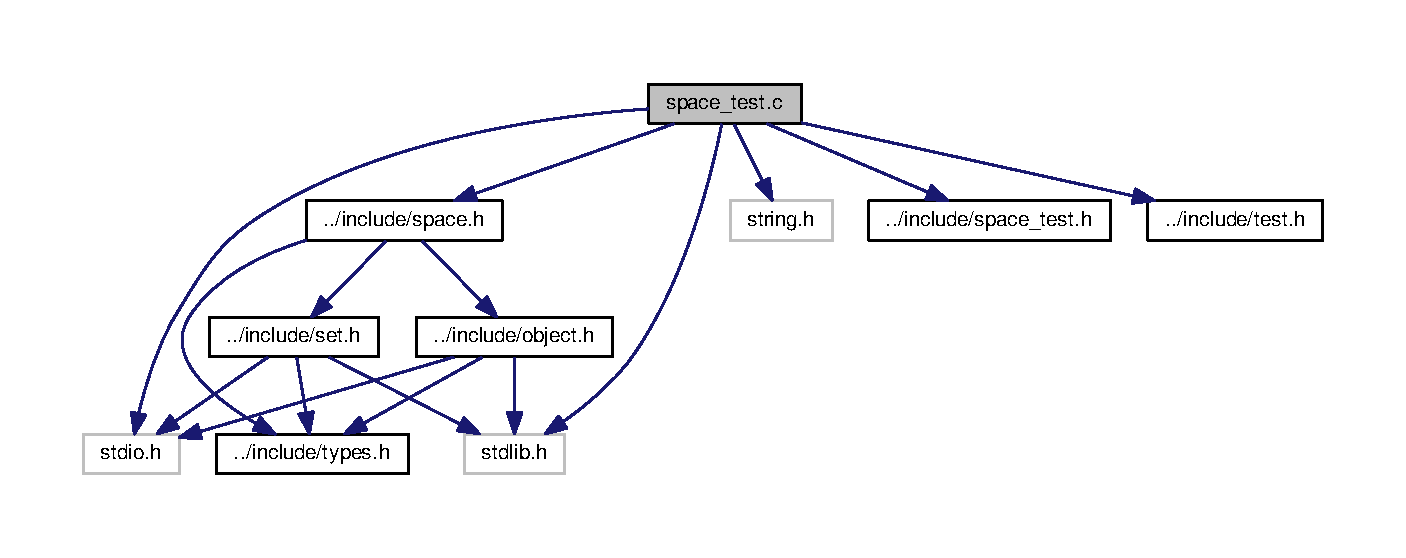
\includegraphics[width=350pt]{space__test_8c__incl}
\end{center}
\end{figure}
\subsection*{Macros}
\begin{DoxyCompactItemize}
\item 
\mbox{\Hypertarget{space__test_8c_a2a77d2f2c5b698c69c19e1f8782bf709}\label{space__test_8c_a2a77d2f2c5b698c69c19e1f8782bf709}} 
\#define {\bfseries M\+A\+X\+\_\+\+T\+E\+S\+TS}~28
\end{DoxyCompactItemize}
\subsection*{Functions}
\begin{DoxyCompactItemize}
\item 
int \hyperlink{space__test_8c_a3c04138a5bfe5d72780bb7e82a18e627}{main} (int argc, char $\ast$$\ast$argv)
\begin{DoxyCompactList}\small\item\em Funcion principal de pruebas para el modulo Space. \end{DoxyCompactList}\item 
void \hyperlink{space__test_8c_a69278cc022dc5688d4725f8d36317b30}{test1\+\_\+space\+\_\+create} ()
\item 
void \hyperlink{space__test_8c_a012cd3cf37a8d91e2d7098a264c29d65}{test2\+\_\+space\+\_\+create} ()
\item 
void \hyperlink{space__test_8c_a2569bab6cfeec15f722d232bb8c78c9e}{test1\+\_\+space\+\_\+set\+\_\+name} ()
\item 
void \hyperlink{space__test_8c_a5a868ba017602ba6b58447cb394e81a6}{test2\+\_\+space\+\_\+set\+\_\+name} ()
\item 
void \hyperlink{space__test_8c_aa24a337830006e33706ab6ac1c416b47}{test3\+\_\+space\+\_\+set\+\_\+name} ()
\item 
\mbox{\Hypertarget{space__test_8c_a3d3457a89f705948102cf1e5d4a7b45b}\label{space__test_8c_a3d3457a89f705948102cf1e5d4a7b45b}} 
void {\bfseries test1\+\_\+space\+\_\+set\+\_\+north} ()
\item 
\mbox{\Hypertarget{space__test_8c_a3bc7fe26c1e36ffd195099a9983206e1}\label{space__test_8c_a3bc7fe26c1e36ffd195099a9983206e1}} 
void {\bfseries test2\+\_\+space\+\_\+set\+\_\+north} ()
\item 
\mbox{\Hypertarget{space__test_8c_a21938e16547b3080e9251f960117a859}\label{space__test_8c_a21938e16547b3080e9251f960117a859}} 
void {\bfseries test1\+\_\+space\+\_\+set\+\_\+south} ()
\item 
\mbox{\Hypertarget{space__test_8c_ac9f950741f12ccfcc5ad5d9e71d3d90a}\label{space__test_8c_ac9f950741f12ccfcc5ad5d9e71d3d90a}} 
void {\bfseries test2\+\_\+space\+\_\+set\+\_\+south} ()
\item 
\mbox{\Hypertarget{space__test_8c_ab1f093af4be3ca8e525d0517cc846f47}\label{space__test_8c_ab1f093af4be3ca8e525d0517cc846f47}} 
void {\bfseries test1\+\_\+space\+\_\+set\+\_\+east} ()
\item 
\mbox{\Hypertarget{space__test_8c_a5df66d103388be4518c379b224f53770}\label{space__test_8c_a5df66d103388be4518c379b224f53770}} 
void {\bfseries test2\+\_\+space\+\_\+set\+\_\+east} ()
\item 
\mbox{\Hypertarget{space__test_8c_ab680a8797f793dffd58546074b87d21f}\label{space__test_8c_ab680a8797f793dffd58546074b87d21f}} 
void {\bfseries test1\+\_\+space\+\_\+set\+\_\+west} ()
\item 
\mbox{\Hypertarget{space__test_8c_aa51b05ffd99b7bbd8f2dfc23c8f85870}\label{space__test_8c_aa51b05ffd99b7bbd8f2dfc23c8f85870}} 
void {\bfseries test2\+\_\+space\+\_\+set\+\_\+west} ()
\item 
\mbox{\Hypertarget{space__test_8c_a208ae9352ff979024f6ebef4e791356a}\label{space__test_8c_a208ae9352ff979024f6ebef4e791356a}} 
void {\bfseries test1\+\_\+space\+\_\+set\+\_\+object} ()
\item 
\mbox{\Hypertarget{space__test_8c_a6349e2b547c71dee23b96d8bbf7a1806}\label{space__test_8c_a6349e2b547c71dee23b96d8bbf7a1806}} 
void {\bfseries test2\+\_\+space\+\_\+set\+\_\+object} ()
\item 
\mbox{\Hypertarget{space__test_8c_ad12c42523c517507566c5c68b1527689}\label{space__test_8c_ad12c42523c517507566c5c68b1527689}} 
void {\bfseries test1\+\_\+space\+\_\+get\+\_\+name} ()
\item 
\mbox{\Hypertarget{space__test_8c_aee88ed31c63efc674051a4563aed86e2}\label{space__test_8c_aee88ed31c63efc674051a4563aed86e2}} 
void {\bfseries test2\+\_\+space\+\_\+get\+\_\+name} ()
\item 
\mbox{\Hypertarget{space__test_8c_a4a1ca89fa511c04bb07c14edb19c17ba}\label{space__test_8c_a4a1ca89fa511c04bb07c14edb19c17ba}} 
void {\bfseries test1\+\_\+space\+\_\+get\+\_\+object} ()
\item 
\mbox{\Hypertarget{space__test_8c_a0fe857c34f691aaba197d03315c3955f}\label{space__test_8c_a0fe857c34f691aaba197d03315c3955f}} 
void {\bfseries test2\+\_\+space\+\_\+get\+\_\+object} ()
\item 
\mbox{\Hypertarget{space__test_8c_aeeb8a439375d69bc1f0ef494f97f5f68}\label{space__test_8c_aeeb8a439375d69bc1f0ef494f97f5f68}} 
void {\bfseries test3\+\_\+space\+\_\+get\+\_\+object} ()
\item 
\mbox{\Hypertarget{space__test_8c_a3a87f1e1e173d622bfbd3bcd14e060ca}\label{space__test_8c_a3a87f1e1e173d622bfbd3bcd14e060ca}} 
void {\bfseries test1\+\_\+space\+\_\+get\+\_\+north} ()
\item 
\mbox{\Hypertarget{space__test_8c_a61891c9cebb9d26dc9f149ad8341517c}\label{space__test_8c_a61891c9cebb9d26dc9f149ad8341517c}} 
void {\bfseries test2\+\_\+space\+\_\+get\+\_\+north} ()
\item 
\mbox{\Hypertarget{space__test_8c_a8e345065f58565e131bdb3a9d0096ed5}\label{space__test_8c_a8e345065f58565e131bdb3a9d0096ed5}} 
void {\bfseries test1\+\_\+space\+\_\+get\+\_\+south} ()
\item 
\mbox{\Hypertarget{space__test_8c_a40fe07c07c1069023b362a9e506c4c59}\label{space__test_8c_a40fe07c07c1069023b362a9e506c4c59}} 
void {\bfseries test2\+\_\+space\+\_\+get\+\_\+south} ()
\item 
\mbox{\Hypertarget{space__test_8c_a354adb2722b06ec65b7212d2736d6417}\label{space__test_8c_a354adb2722b06ec65b7212d2736d6417}} 
void {\bfseries test1\+\_\+space\+\_\+get\+\_\+east} ()
\item 
\mbox{\Hypertarget{space__test_8c_a249293510e61c6d5465f52c14343d02b}\label{space__test_8c_a249293510e61c6d5465f52c14343d02b}} 
void {\bfseries test2\+\_\+space\+\_\+get\+\_\+east} ()
\item 
\mbox{\Hypertarget{space__test_8c_a1f08c6866885bfc093717f57b1b86539}\label{space__test_8c_a1f08c6866885bfc093717f57b1b86539}} 
void {\bfseries test1\+\_\+space\+\_\+get\+\_\+west} ()
\item 
\mbox{\Hypertarget{space__test_8c_af1cf02b01c007aec0684186b39666c32}\label{space__test_8c_af1cf02b01c007aec0684186b39666c32}} 
void {\bfseries test2\+\_\+space\+\_\+get\+\_\+west} ()
\item 
\mbox{\Hypertarget{space__test_8c_a920df9e02482f4f1e6a5ebcaec523860}\label{space__test_8c_a920df9e02482f4f1e6a5ebcaec523860}} 
void {\bfseries test1\+\_\+space\+\_\+get\+\_\+id} ()
\item 
\mbox{\Hypertarget{space__test_8c_af9087176b0d3c41d83a17a4918b13e31}\label{space__test_8c_af9087176b0d3c41d83a17a4918b13e31}} 
void {\bfseries test2\+\_\+space\+\_\+get\+\_\+id} ()
\end{DoxyCompactItemize}


\subsection{Detailed Description}
It tests space module. 



\subsection{Function Documentation}
\mbox{\Hypertarget{space__test_8c_a3c04138a5bfe5d72780bb7e82a18e627}\label{space__test_8c_a3c04138a5bfe5d72780bb7e82a18e627}} 
\index{space\+\_\+test.\+c@{space\+\_\+test.\+c}!main@{main}}
\index{main@{main}!space\+\_\+test.\+c@{space\+\_\+test.\+c}}
\subsubsection{\texorpdfstring{main()}{main()}}
{\footnotesize\ttfamily int main (\begin{DoxyParamCaption}\item[{int}]{argc,  }\item[{char $\ast$$\ast$}]{argv }\end{DoxyParamCaption})}



Funcion principal de pruebas para el modulo Space. 

Dos modos de ejecucion\+: 1.-\/\+Si se ejecuta sin parametros se ejecutan todas las pruebas 2.-\/\+Si se ejecuta con un numero entre 1 y el numero de pruebas solo ejecuta la prueba indicada \mbox{\Hypertarget{space__test_8c_a69278cc022dc5688d4725f8d36317b30}\label{space__test_8c_a69278cc022dc5688d4725f8d36317b30}} 
\index{space\+\_\+test.\+c@{space\+\_\+test.\+c}!test1\+\_\+space\+\_\+create@{test1\+\_\+space\+\_\+create}}
\index{test1\+\_\+space\+\_\+create@{test1\+\_\+space\+\_\+create}!space\+\_\+test.\+c@{space\+\_\+test.\+c}}
\subsubsection{\texorpdfstring{test1\+\_\+space\+\_\+create()}{test1\_space\_create()}}
{\footnotesize\ttfamily void test1\+\_\+space\+\_\+create (\begin{DoxyParamCaption}{ }\end{DoxyParamCaption})}

\begin{DoxyRefDesc}{Test}
\item[\hyperlink{test__test000001}{Test}]Prueba la función de creación de un espacio \end{DoxyRefDesc}
\begin{DoxyPrecond}{Precondition}
Un identificador como parámetro 
\end{DoxyPrecond}
\begin{DoxyPostcond}{Postcondition}
Un puntero no nulo al espacio creado 
\end{DoxyPostcond}
\mbox{\Hypertarget{space__test_8c_a2569bab6cfeec15f722d232bb8c78c9e}\label{space__test_8c_a2569bab6cfeec15f722d232bb8c78c9e}} 
\index{space\+\_\+test.\+c@{space\+\_\+test.\+c}!test1\+\_\+space\+\_\+set\+\_\+name@{test1\+\_\+space\+\_\+set\+\_\+name}}
\index{test1\+\_\+space\+\_\+set\+\_\+name@{test1\+\_\+space\+\_\+set\+\_\+name}!space\+\_\+test.\+c@{space\+\_\+test.\+c}}
\subsubsection{\texorpdfstring{test1\+\_\+space\+\_\+set\+\_\+name()}{test1\_space\_set\_name()}}
{\footnotesize\ttfamily void test1\+\_\+space\+\_\+set\+\_\+name (\begin{DoxyParamCaption}{ }\end{DoxyParamCaption})}

\begin{DoxyRefDesc}{Test}
\item[\hyperlink{test__test000003}{Test}]Prueba la función para establecer el nombre de un espacio \end{DoxyRefDesc}
\begin{DoxyPrecond}{Precondition}
Nombre que establecer al espacio 
\end{DoxyPrecond}
\begin{DoxyPostcond}{Postcondition}
La salida debe ser OK 
\end{DoxyPostcond}
\mbox{\Hypertarget{space__test_8c_a012cd3cf37a8d91e2d7098a264c29d65}\label{space__test_8c_a012cd3cf37a8d91e2d7098a264c29d65}} 
\index{space\+\_\+test.\+c@{space\+\_\+test.\+c}!test2\+\_\+space\+\_\+create@{test2\+\_\+space\+\_\+create}}
\index{test2\+\_\+space\+\_\+create@{test2\+\_\+space\+\_\+create}!space\+\_\+test.\+c@{space\+\_\+test.\+c}}
\subsubsection{\texorpdfstring{test2\+\_\+space\+\_\+create()}{test2\_space\_create()}}
{\footnotesize\ttfamily void test2\+\_\+space\+\_\+create (\begin{DoxyParamCaption}{ }\end{DoxyParamCaption})}

\begin{DoxyRefDesc}{Test}
\item[\hyperlink{test__test000002}{Test}]Prueba la función de creación de un espacio \end{DoxyRefDesc}
\begin{DoxyPrecond}{Precondition}
Un identificador como parámetro 
\end{DoxyPrecond}
\begin{DoxyPostcond}{Postcondition}
El identificador del espacio es el introducido 
\end{DoxyPostcond}
\mbox{\Hypertarget{space__test_8c_a5a868ba017602ba6b58447cb394e81a6}\label{space__test_8c_a5a868ba017602ba6b58447cb394e81a6}} 
\index{space\+\_\+test.\+c@{space\+\_\+test.\+c}!test2\+\_\+space\+\_\+set\+\_\+name@{test2\+\_\+space\+\_\+set\+\_\+name}}
\index{test2\+\_\+space\+\_\+set\+\_\+name@{test2\+\_\+space\+\_\+set\+\_\+name}!space\+\_\+test.\+c@{space\+\_\+test.\+c}}
\subsubsection{\texorpdfstring{test2\+\_\+space\+\_\+set\+\_\+name()}{test2\_space\_set\_name()}}
{\footnotesize\ttfamily void test2\+\_\+space\+\_\+set\+\_\+name (\begin{DoxyParamCaption}{ }\end{DoxyParamCaption})}

\begin{DoxyRefDesc}{Test}
\item[\hyperlink{test__test000004}{Test}]Prueba la función para establecer el nombre de un espacio \end{DoxyRefDesc}
\begin{DoxyPrecond}{Precondition}
El espacio al que establecer el nombre es un puntero a N\+U\+LL 
\end{DoxyPrecond}
\begin{DoxyPostcond}{Postcondition}
La salida debe ser E\+R\+R\+OR 
\end{DoxyPostcond}
\mbox{\Hypertarget{space__test_8c_aa24a337830006e33706ab6ac1c416b47}\label{space__test_8c_aa24a337830006e33706ab6ac1c416b47}} 
\index{space\+\_\+test.\+c@{space\+\_\+test.\+c}!test3\+\_\+space\+\_\+set\+\_\+name@{test3\+\_\+space\+\_\+set\+\_\+name}}
\index{test3\+\_\+space\+\_\+set\+\_\+name@{test3\+\_\+space\+\_\+set\+\_\+name}!space\+\_\+test.\+c@{space\+\_\+test.\+c}}
\subsubsection{\texorpdfstring{test3\+\_\+space\+\_\+set\+\_\+name()}{test3\_space\_set\_name()}}
{\footnotesize\ttfamily void test3\+\_\+space\+\_\+set\+\_\+name (\begin{DoxyParamCaption}{ }\end{DoxyParamCaption})}

\begin{DoxyRefDesc}{Test}
\item[\hyperlink{test__test000005}{Test}]Prueba la función para establecer el nombre de un espacio \end{DoxyRefDesc}
\begin{DoxyPrecond}{Precondition}
El espacio es un puntero no N\+U\+LL, pero el nombre a establecer es N\+U\+LL 
\end{DoxyPrecond}
\begin{DoxyPostcond}{Postcondition}
La salida debe ser E\+R\+R\+OR 
\end{DoxyPostcond}

\hypertarget{space__test_8h}{}\section{space\+\_\+test.\+h File Reference}
\label{space__test_8h}\index{space\+\_\+test.\+h@{space\+\_\+test.\+h}}


It declares the tests for the space module.  


This graph shows which files directly or indirectly include this file\+:\nopagebreak
\begin{figure}[H]
\begin{center}
\leavevmode
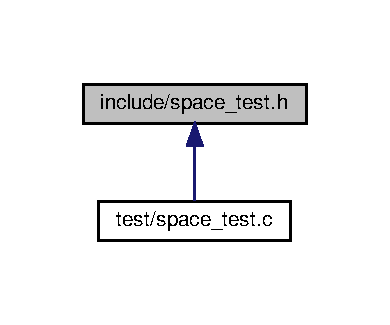
\includegraphics[width=152pt]{space__test_8h__dep__incl}
\end{center}
\end{figure}
\subsection*{Functions}
\begin{DoxyCompactItemize}
\item 
void \hyperlink{space__test_8h_a69278cc022dc5688d4725f8d36317b30}{test1\+\_\+space\+\_\+create} ()
\item 
void \hyperlink{space__test_8h_a012cd3cf37a8d91e2d7098a264c29d65}{test2\+\_\+space\+\_\+create} ()
\item 
void \hyperlink{space__test_8h_a2569bab6cfeec15f722d232bb8c78c9e}{test1\+\_\+space\+\_\+set\+\_\+name} ()
\item 
void \hyperlink{space__test_8h_a5a868ba017602ba6b58447cb394e81a6}{test2\+\_\+space\+\_\+set\+\_\+name} ()
\item 
void \hyperlink{space__test_8h_aa24a337830006e33706ab6ac1c416b47}{test3\+\_\+space\+\_\+set\+\_\+name} ()
\item 
void \hyperlink{space__test_8h_a3d3457a89f705948102cf1e5d4a7b45b}{test1\+\_\+space\+\_\+set\+\_\+north} ()
\item 
void \hyperlink{space__test_8h_a3bc7fe26c1e36ffd195099a9983206e1}{test2\+\_\+space\+\_\+set\+\_\+north} ()
\item 
void \hyperlink{space__test_8h_ac2961dcc4d7645660ca6953a70315b0a}{test3\+\_\+space\+\_\+set\+\_\+north} ()
\item 
void \hyperlink{space__test_8h_ae0c160dea7603545b4f0b982a34aaed7}{test4\+\_\+space\+\_\+set\+\_\+north} ()
\item 
void \hyperlink{space__test_8h_a21938e16547b3080e9251f960117a859}{test1\+\_\+space\+\_\+set\+\_\+south} ()
\item 
void \hyperlink{space__test_8h_ac9f950741f12ccfcc5ad5d9e71d3d90a}{test2\+\_\+space\+\_\+set\+\_\+south} ()
\item 
void \hyperlink{space__test_8h_ab2626f0045b225c79a8c5d56298e2065}{test3\+\_\+space\+\_\+set\+\_\+south} ()
\item 
void \hyperlink{space__test_8h_aa758704ed422a39c8f7e1932c4e03cb3}{test4\+\_\+space\+\_\+set\+\_\+south} ()
\item 
void \hyperlink{space__test_8h_ab1f093af4be3ca8e525d0517cc846f47}{test1\+\_\+space\+\_\+set\+\_\+east} ()
\item 
void \hyperlink{space__test_8h_a5df66d103388be4518c379b224f53770}{test2\+\_\+space\+\_\+set\+\_\+east} ()
\item 
void \hyperlink{space__test_8h_adf98486d8745110660515d14b71b5656}{test3\+\_\+space\+\_\+set\+\_\+east} ()
\item 
void \hyperlink{space__test_8h_a10eb50d23f317e89c3f54772a664d0ad}{test4\+\_\+space\+\_\+set\+\_\+east} ()
\item 
void \hyperlink{space__test_8h_ab680a8797f793dffd58546074b87d21f}{test1\+\_\+space\+\_\+set\+\_\+west} ()
\item 
void \hyperlink{space__test_8h_aa51b05ffd99b7bbd8f2dfc23c8f85870}{test2\+\_\+space\+\_\+set\+\_\+west} ()
\item 
void \hyperlink{space__test_8h_a8150758940559ef958649a2fab36bee0}{test3\+\_\+space\+\_\+set\+\_\+west} ()
\item 
void \hyperlink{space__test_8h_a7bfef2166b80d6e2932334c0adbaa597}{test4\+\_\+space\+\_\+set\+\_\+west} ()
\item 
void \hyperlink{space__test_8h_a920df9e02482f4f1e6a5ebcaec523860}{test1\+\_\+space\+\_\+get\+\_\+id} ()
\item 
void \hyperlink{space__test_8h_af9087176b0d3c41d83a17a4918b13e31}{test2\+\_\+space\+\_\+get\+\_\+id} ()
\item 
void \hyperlink{space__test_8h_a208ae9352ff979024f6ebef4e791356a}{test1\+\_\+space\+\_\+set\+\_\+object} ()
\item 
void \hyperlink{space__test_8h_a6349e2b547c71dee23b96d8bbf7a1806}{test2\+\_\+space\+\_\+set\+\_\+object} ()
\item 
void \hyperlink{space__test_8h_ad12c42523c517507566c5c68b1527689}{test1\+\_\+space\+\_\+get\+\_\+name} ()
\item 
void \hyperlink{space__test_8h_aee88ed31c63efc674051a4563aed86e2}{test2\+\_\+space\+\_\+get\+\_\+name} ()
\item 
void \hyperlink{space__test_8h_a3a87f1e1e173d622bfbd3bcd14e060ca}{test1\+\_\+space\+\_\+get\+\_\+north} ()
\item 
void \hyperlink{space__test_8h_a61891c9cebb9d26dc9f149ad8341517c}{test2\+\_\+space\+\_\+get\+\_\+north} ()
\item 
void \hyperlink{space__test_8h_a8e345065f58565e131bdb3a9d0096ed5}{test1\+\_\+space\+\_\+get\+\_\+south} ()
\item 
void \hyperlink{space__test_8h_a40fe07c07c1069023b362a9e506c4c59}{test2\+\_\+space\+\_\+get\+\_\+south} ()
\item 
void \hyperlink{space__test_8h_a354adb2722b06ec65b7212d2736d6417}{test1\+\_\+space\+\_\+get\+\_\+east} ()
\item 
void \hyperlink{space__test_8h_a249293510e61c6d5465f52c14343d02b}{test2\+\_\+space\+\_\+get\+\_\+east} ()
\item 
void \hyperlink{space__test_8h_a1f08c6866885bfc093717f57b1b86539}{test1\+\_\+space\+\_\+get\+\_\+west} ()
\item 
void \hyperlink{space__test_8h_af1cf02b01c007aec0684186b39666c32}{test2\+\_\+space\+\_\+get\+\_\+west} ()
\item 
void \hyperlink{space__test_8h_a4a1ca89fa511c04bb07c14edb19c17ba}{test1\+\_\+space\+\_\+get\+\_\+object} ()
\item 
void \hyperlink{space__test_8h_a0fe857c34f691aaba197d03315c3955f}{test2\+\_\+space\+\_\+get\+\_\+object} ()
\item 
void \hyperlink{space__test_8h_aeeb8a439375d69bc1f0ef494f97f5f68}{test3\+\_\+space\+\_\+get\+\_\+object} ()
\end{DoxyCompactItemize}


\subsection{Detailed Description}
It declares the tests for the space module. 

\begin{DoxyAuthor}{Author}
Profesores Pprog 
\end{DoxyAuthor}
\begin{DoxyCopyright}{Copyright}
G\+NU Public License 
\end{DoxyCopyright}


\subsection{Function Documentation}
\index{space\+\_\+test.\+h@{space\+\_\+test.\+h}!test1\+\_\+space\+\_\+create@{test1\+\_\+space\+\_\+create}}
\index{test1\+\_\+space\+\_\+create@{test1\+\_\+space\+\_\+create}!space\+\_\+test.\+h@{space\+\_\+test.\+h}}
\subsubsection[{\texorpdfstring{test1\+\_\+space\+\_\+create()}{test1_space_create()}}]{\setlength{\rightskip}{0pt plus 5cm}void test1\+\_\+space\+\_\+create (
\begin{DoxyParamCaption}
{}
\end{DoxyParamCaption}
)}\hypertarget{space__test_8h_a69278cc022dc5688d4725f8d36317b30}{}\label{space__test_8h_a69278cc022dc5688d4725f8d36317b30}
\begin{DoxyRefDesc}{Test}
\item[\hyperlink{test__test000001}{Test}]Prueba la función de creación de un espacio \end{DoxyRefDesc}
\begin{DoxyPrecond}{Precondition}
Un identificador como parámetro 
\end{DoxyPrecond}
\begin{DoxyPostcond}{Postcondition}
Un puntero no nulo al espacio creado 
\end{DoxyPostcond}
\index{space\+\_\+test.\+h@{space\+\_\+test.\+h}!test1\+\_\+space\+\_\+get\+\_\+east@{test1\+\_\+space\+\_\+get\+\_\+east}}
\index{test1\+\_\+space\+\_\+get\+\_\+east@{test1\+\_\+space\+\_\+get\+\_\+east}!space\+\_\+test.\+h@{space\+\_\+test.\+h}}
\subsubsection[{\texorpdfstring{test1\+\_\+space\+\_\+get\+\_\+east()}{test1_space_get_east()}}]{\setlength{\rightskip}{0pt plus 5cm}void test1\+\_\+space\+\_\+get\+\_\+east (
\begin{DoxyParamCaption}
{}
\end{DoxyParamCaption}
)}\hypertarget{space__test_8h_a354adb2722b06ec65b7212d2736d6417}{}\label{space__test_8h_a354adb2722b06ec65b7212d2736d6417}
\index{space\+\_\+test.\+h@{space\+\_\+test.\+h}!test1\+\_\+space\+\_\+get\+\_\+id@{test1\+\_\+space\+\_\+get\+\_\+id}}
\index{test1\+\_\+space\+\_\+get\+\_\+id@{test1\+\_\+space\+\_\+get\+\_\+id}!space\+\_\+test.\+h@{space\+\_\+test.\+h}}
\subsubsection[{\texorpdfstring{test1\+\_\+space\+\_\+get\+\_\+id()}{test1_space_get_id()}}]{\setlength{\rightskip}{0pt plus 5cm}void test1\+\_\+space\+\_\+get\+\_\+id (
\begin{DoxyParamCaption}
{}
\end{DoxyParamCaption}
)}\hypertarget{space__test_8h_a920df9e02482f4f1e6a5ebcaec523860}{}\label{space__test_8h_a920df9e02482f4f1e6a5ebcaec523860}
\index{space\+\_\+test.\+h@{space\+\_\+test.\+h}!test1\+\_\+space\+\_\+get\+\_\+name@{test1\+\_\+space\+\_\+get\+\_\+name}}
\index{test1\+\_\+space\+\_\+get\+\_\+name@{test1\+\_\+space\+\_\+get\+\_\+name}!space\+\_\+test.\+h@{space\+\_\+test.\+h}}
\subsubsection[{\texorpdfstring{test1\+\_\+space\+\_\+get\+\_\+name()}{test1_space_get_name()}}]{\setlength{\rightskip}{0pt plus 5cm}void test1\+\_\+space\+\_\+get\+\_\+name (
\begin{DoxyParamCaption}
{}
\end{DoxyParamCaption}
)}\hypertarget{space__test_8h_ad12c42523c517507566c5c68b1527689}{}\label{space__test_8h_ad12c42523c517507566c5c68b1527689}
\index{space\+\_\+test.\+h@{space\+\_\+test.\+h}!test1\+\_\+space\+\_\+get\+\_\+north@{test1\+\_\+space\+\_\+get\+\_\+north}}
\index{test1\+\_\+space\+\_\+get\+\_\+north@{test1\+\_\+space\+\_\+get\+\_\+north}!space\+\_\+test.\+h@{space\+\_\+test.\+h}}
\subsubsection[{\texorpdfstring{test1\+\_\+space\+\_\+get\+\_\+north()}{test1_space_get_north()}}]{\setlength{\rightskip}{0pt plus 5cm}void test1\+\_\+space\+\_\+get\+\_\+north (
\begin{DoxyParamCaption}
{}
\end{DoxyParamCaption}
)}\hypertarget{space__test_8h_a3a87f1e1e173d622bfbd3bcd14e060ca}{}\label{space__test_8h_a3a87f1e1e173d622bfbd3bcd14e060ca}
\index{space\+\_\+test.\+h@{space\+\_\+test.\+h}!test1\+\_\+space\+\_\+get\+\_\+object@{test1\+\_\+space\+\_\+get\+\_\+object}}
\index{test1\+\_\+space\+\_\+get\+\_\+object@{test1\+\_\+space\+\_\+get\+\_\+object}!space\+\_\+test.\+h@{space\+\_\+test.\+h}}
\subsubsection[{\texorpdfstring{test1\+\_\+space\+\_\+get\+\_\+object()}{test1_space_get_object()}}]{\setlength{\rightskip}{0pt plus 5cm}void test1\+\_\+space\+\_\+get\+\_\+object (
\begin{DoxyParamCaption}
{}
\end{DoxyParamCaption}
)}\hypertarget{space__test_8h_a4a1ca89fa511c04bb07c14edb19c17ba}{}\label{space__test_8h_a4a1ca89fa511c04bb07c14edb19c17ba}
\index{space\+\_\+test.\+h@{space\+\_\+test.\+h}!test1\+\_\+space\+\_\+get\+\_\+south@{test1\+\_\+space\+\_\+get\+\_\+south}}
\index{test1\+\_\+space\+\_\+get\+\_\+south@{test1\+\_\+space\+\_\+get\+\_\+south}!space\+\_\+test.\+h@{space\+\_\+test.\+h}}
\subsubsection[{\texorpdfstring{test1\+\_\+space\+\_\+get\+\_\+south()}{test1_space_get_south()}}]{\setlength{\rightskip}{0pt plus 5cm}void test1\+\_\+space\+\_\+get\+\_\+south (
\begin{DoxyParamCaption}
{}
\end{DoxyParamCaption}
)}\hypertarget{space__test_8h_a8e345065f58565e131bdb3a9d0096ed5}{}\label{space__test_8h_a8e345065f58565e131bdb3a9d0096ed5}
\index{space\+\_\+test.\+h@{space\+\_\+test.\+h}!test1\+\_\+space\+\_\+get\+\_\+west@{test1\+\_\+space\+\_\+get\+\_\+west}}
\index{test1\+\_\+space\+\_\+get\+\_\+west@{test1\+\_\+space\+\_\+get\+\_\+west}!space\+\_\+test.\+h@{space\+\_\+test.\+h}}
\subsubsection[{\texorpdfstring{test1\+\_\+space\+\_\+get\+\_\+west()}{test1_space_get_west()}}]{\setlength{\rightskip}{0pt plus 5cm}void test1\+\_\+space\+\_\+get\+\_\+west (
\begin{DoxyParamCaption}
{}
\end{DoxyParamCaption}
)}\hypertarget{space__test_8h_a1f08c6866885bfc093717f57b1b86539}{}\label{space__test_8h_a1f08c6866885bfc093717f57b1b86539}
\index{space\+\_\+test.\+h@{space\+\_\+test.\+h}!test1\+\_\+space\+\_\+set\+\_\+east@{test1\+\_\+space\+\_\+set\+\_\+east}}
\index{test1\+\_\+space\+\_\+set\+\_\+east@{test1\+\_\+space\+\_\+set\+\_\+east}!space\+\_\+test.\+h@{space\+\_\+test.\+h}}
\subsubsection[{\texorpdfstring{test1\+\_\+space\+\_\+set\+\_\+east()}{test1_space_set_east()}}]{\setlength{\rightskip}{0pt plus 5cm}void test1\+\_\+space\+\_\+set\+\_\+east (
\begin{DoxyParamCaption}
{}
\end{DoxyParamCaption}
)}\hypertarget{space__test_8h_ab1f093af4be3ca8e525d0517cc846f47}{}\label{space__test_8h_ab1f093af4be3ca8e525d0517cc846f47}
\index{space\+\_\+test.\+h@{space\+\_\+test.\+h}!test1\+\_\+space\+\_\+set\+\_\+name@{test1\+\_\+space\+\_\+set\+\_\+name}}
\index{test1\+\_\+space\+\_\+set\+\_\+name@{test1\+\_\+space\+\_\+set\+\_\+name}!space\+\_\+test.\+h@{space\+\_\+test.\+h}}
\subsubsection[{\texorpdfstring{test1\+\_\+space\+\_\+set\+\_\+name()}{test1_space_set_name()}}]{\setlength{\rightskip}{0pt plus 5cm}void test1\+\_\+space\+\_\+set\+\_\+name (
\begin{DoxyParamCaption}
{}
\end{DoxyParamCaption}
)}\hypertarget{space__test_8h_a2569bab6cfeec15f722d232bb8c78c9e}{}\label{space__test_8h_a2569bab6cfeec15f722d232bb8c78c9e}
\begin{DoxyRefDesc}{Test}
\item[\hyperlink{test__test000003}{Test}]Prueba la función para establecer el nombre de un espacio \end{DoxyRefDesc}
\begin{DoxyPrecond}{Precondition}
Nombre que establecer al espacio 
\end{DoxyPrecond}
\begin{DoxyPostcond}{Postcondition}
La salida debe ser OK 
\end{DoxyPostcond}
\index{space\+\_\+test.\+h@{space\+\_\+test.\+h}!test1\+\_\+space\+\_\+set\+\_\+north@{test1\+\_\+space\+\_\+set\+\_\+north}}
\index{test1\+\_\+space\+\_\+set\+\_\+north@{test1\+\_\+space\+\_\+set\+\_\+north}!space\+\_\+test.\+h@{space\+\_\+test.\+h}}
\subsubsection[{\texorpdfstring{test1\+\_\+space\+\_\+set\+\_\+north()}{test1_space_set_north()}}]{\setlength{\rightskip}{0pt plus 5cm}void test1\+\_\+space\+\_\+set\+\_\+north (
\begin{DoxyParamCaption}
{}
\end{DoxyParamCaption}
)}\hypertarget{space__test_8h_a3d3457a89f705948102cf1e5d4a7b45b}{}\label{space__test_8h_a3d3457a89f705948102cf1e5d4a7b45b}
\index{space\+\_\+test.\+h@{space\+\_\+test.\+h}!test1\+\_\+space\+\_\+set\+\_\+object@{test1\+\_\+space\+\_\+set\+\_\+object}}
\index{test1\+\_\+space\+\_\+set\+\_\+object@{test1\+\_\+space\+\_\+set\+\_\+object}!space\+\_\+test.\+h@{space\+\_\+test.\+h}}
\subsubsection[{\texorpdfstring{test1\+\_\+space\+\_\+set\+\_\+object()}{test1_space_set_object()}}]{\setlength{\rightskip}{0pt plus 5cm}void test1\+\_\+space\+\_\+set\+\_\+object (
\begin{DoxyParamCaption}
{}
\end{DoxyParamCaption}
)}\hypertarget{space__test_8h_a208ae9352ff979024f6ebef4e791356a}{}\label{space__test_8h_a208ae9352ff979024f6ebef4e791356a}
\index{space\+\_\+test.\+h@{space\+\_\+test.\+h}!test1\+\_\+space\+\_\+set\+\_\+south@{test1\+\_\+space\+\_\+set\+\_\+south}}
\index{test1\+\_\+space\+\_\+set\+\_\+south@{test1\+\_\+space\+\_\+set\+\_\+south}!space\+\_\+test.\+h@{space\+\_\+test.\+h}}
\subsubsection[{\texorpdfstring{test1\+\_\+space\+\_\+set\+\_\+south()}{test1_space_set_south()}}]{\setlength{\rightskip}{0pt plus 5cm}void test1\+\_\+space\+\_\+set\+\_\+south (
\begin{DoxyParamCaption}
{}
\end{DoxyParamCaption}
)}\hypertarget{space__test_8h_a21938e16547b3080e9251f960117a859}{}\label{space__test_8h_a21938e16547b3080e9251f960117a859}
\index{space\+\_\+test.\+h@{space\+\_\+test.\+h}!test1\+\_\+space\+\_\+set\+\_\+west@{test1\+\_\+space\+\_\+set\+\_\+west}}
\index{test1\+\_\+space\+\_\+set\+\_\+west@{test1\+\_\+space\+\_\+set\+\_\+west}!space\+\_\+test.\+h@{space\+\_\+test.\+h}}
\subsubsection[{\texorpdfstring{test1\+\_\+space\+\_\+set\+\_\+west()}{test1_space_set_west()}}]{\setlength{\rightskip}{0pt plus 5cm}void test1\+\_\+space\+\_\+set\+\_\+west (
\begin{DoxyParamCaption}
{}
\end{DoxyParamCaption}
)}\hypertarget{space__test_8h_ab680a8797f793dffd58546074b87d21f}{}\label{space__test_8h_ab680a8797f793dffd58546074b87d21f}
\index{space\+\_\+test.\+h@{space\+\_\+test.\+h}!test2\+\_\+space\+\_\+create@{test2\+\_\+space\+\_\+create}}
\index{test2\+\_\+space\+\_\+create@{test2\+\_\+space\+\_\+create}!space\+\_\+test.\+h@{space\+\_\+test.\+h}}
\subsubsection[{\texorpdfstring{test2\+\_\+space\+\_\+create()}{test2_space_create()}}]{\setlength{\rightskip}{0pt plus 5cm}void test2\+\_\+space\+\_\+create (
\begin{DoxyParamCaption}
{}
\end{DoxyParamCaption}
)}\hypertarget{space__test_8h_a012cd3cf37a8d91e2d7098a264c29d65}{}\label{space__test_8h_a012cd3cf37a8d91e2d7098a264c29d65}
\begin{DoxyRefDesc}{Test}
\item[\hyperlink{test__test000002}{Test}]Prueba la función de creación de un espacio \end{DoxyRefDesc}
\begin{DoxyPrecond}{Precondition}
Un identificador como parámetro 
\end{DoxyPrecond}
\begin{DoxyPostcond}{Postcondition}
El identificador del espacio es el introducido 
\end{DoxyPostcond}
\index{space\+\_\+test.\+h@{space\+\_\+test.\+h}!test2\+\_\+space\+\_\+get\+\_\+east@{test2\+\_\+space\+\_\+get\+\_\+east}}
\index{test2\+\_\+space\+\_\+get\+\_\+east@{test2\+\_\+space\+\_\+get\+\_\+east}!space\+\_\+test.\+h@{space\+\_\+test.\+h}}
\subsubsection[{\texorpdfstring{test2\+\_\+space\+\_\+get\+\_\+east()}{test2_space_get_east()}}]{\setlength{\rightskip}{0pt plus 5cm}void test2\+\_\+space\+\_\+get\+\_\+east (
\begin{DoxyParamCaption}
{}
\end{DoxyParamCaption}
)}\hypertarget{space__test_8h_a249293510e61c6d5465f52c14343d02b}{}\label{space__test_8h_a249293510e61c6d5465f52c14343d02b}
\index{space\+\_\+test.\+h@{space\+\_\+test.\+h}!test2\+\_\+space\+\_\+get\+\_\+id@{test2\+\_\+space\+\_\+get\+\_\+id}}
\index{test2\+\_\+space\+\_\+get\+\_\+id@{test2\+\_\+space\+\_\+get\+\_\+id}!space\+\_\+test.\+h@{space\+\_\+test.\+h}}
\subsubsection[{\texorpdfstring{test2\+\_\+space\+\_\+get\+\_\+id()}{test2_space_get_id()}}]{\setlength{\rightskip}{0pt plus 5cm}void test2\+\_\+space\+\_\+get\+\_\+id (
\begin{DoxyParamCaption}
{}
\end{DoxyParamCaption}
)}\hypertarget{space__test_8h_af9087176b0d3c41d83a17a4918b13e31}{}\label{space__test_8h_af9087176b0d3c41d83a17a4918b13e31}
\index{space\+\_\+test.\+h@{space\+\_\+test.\+h}!test2\+\_\+space\+\_\+get\+\_\+name@{test2\+\_\+space\+\_\+get\+\_\+name}}
\index{test2\+\_\+space\+\_\+get\+\_\+name@{test2\+\_\+space\+\_\+get\+\_\+name}!space\+\_\+test.\+h@{space\+\_\+test.\+h}}
\subsubsection[{\texorpdfstring{test2\+\_\+space\+\_\+get\+\_\+name()}{test2_space_get_name()}}]{\setlength{\rightskip}{0pt plus 5cm}void test2\+\_\+space\+\_\+get\+\_\+name (
\begin{DoxyParamCaption}
{}
\end{DoxyParamCaption}
)}\hypertarget{space__test_8h_aee88ed31c63efc674051a4563aed86e2}{}\label{space__test_8h_aee88ed31c63efc674051a4563aed86e2}
\index{space\+\_\+test.\+h@{space\+\_\+test.\+h}!test2\+\_\+space\+\_\+get\+\_\+north@{test2\+\_\+space\+\_\+get\+\_\+north}}
\index{test2\+\_\+space\+\_\+get\+\_\+north@{test2\+\_\+space\+\_\+get\+\_\+north}!space\+\_\+test.\+h@{space\+\_\+test.\+h}}
\subsubsection[{\texorpdfstring{test2\+\_\+space\+\_\+get\+\_\+north()}{test2_space_get_north()}}]{\setlength{\rightskip}{0pt plus 5cm}void test2\+\_\+space\+\_\+get\+\_\+north (
\begin{DoxyParamCaption}
{}
\end{DoxyParamCaption}
)}\hypertarget{space__test_8h_a61891c9cebb9d26dc9f149ad8341517c}{}\label{space__test_8h_a61891c9cebb9d26dc9f149ad8341517c}
\index{space\+\_\+test.\+h@{space\+\_\+test.\+h}!test2\+\_\+space\+\_\+get\+\_\+object@{test2\+\_\+space\+\_\+get\+\_\+object}}
\index{test2\+\_\+space\+\_\+get\+\_\+object@{test2\+\_\+space\+\_\+get\+\_\+object}!space\+\_\+test.\+h@{space\+\_\+test.\+h}}
\subsubsection[{\texorpdfstring{test2\+\_\+space\+\_\+get\+\_\+object()}{test2_space_get_object()}}]{\setlength{\rightskip}{0pt plus 5cm}void test2\+\_\+space\+\_\+get\+\_\+object (
\begin{DoxyParamCaption}
{}
\end{DoxyParamCaption}
)}\hypertarget{space__test_8h_a0fe857c34f691aaba197d03315c3955f}{}\label{space__test_8h_a0fe857c34f691aaba197d03315c3955f}
\index{space\+\_\+test.\+h@{space\+\_\+test.\+h}!test2\+\_\+space\+\_\+get\+\_\+south@{test2\+\_\+space\+\_\+get\+\_\+south}}
\index{test2\+\_\+space\+\_\+get\+\_\+south@{test2\+\_\+space\+\_\+get\+\_\+south}!space\+\_\+test.\+h@{space\+\_\+test.\+h}}
\subsubsection[{\texorpdfstring{test2\+\_\+space\+\_\+get\+\_\+south()}{test2_space_get_south()}}]{\setlength{\rightskip}{0pt plus 5cm}void test2\+\_\+space\+\_\+get\+\_\+south (
\begin{DoxyParamCaption}
{}
\end{DoxyParamCaption}
)}\hypertarget{space__test_8h_a40fe07c07c1069023b362a9e506c4c59}{}\label{space__test_8h_a40fe07c07c1069023b362a9e506c4c59}
\index{space\+\_\+test.\+h@{space\+\_\+test.\+h}!test2\+\_\+space\+\_\+get\+\_\+west@{test2\+\_\+space\+\_\+get\+\_\+west}}
\index{test2\+\_\+space\+\_\+get\+\_\+west@{test2\+\_\+space\+\_\+get\+\_\+west}!space\+\_\+test.\+h@{space\+\_\+test.\+h}}
\subsubsection[{\texorpdfstring{test2\+\_\+space\+\_\+get\+\_\+west()}{test2_space_get_west()}}]{\setlength{\rightskip}{0pt plus 5cm}void test2\+\_\+space\+\_\+get\+\_\+west (
\begin{DoxyParamCaption}
{}
\end{DoxyParamCaption}
)}\hypertarget{space__test_8h_af1cf02b01c007aec0684186b39666c32}{}\label{space__test_8h_af1cf02b01c007aec0684186b39666c32}
\index{space\+\_\+test.\+h@{space\+\_\+test.\+h}!test2\+\_\+space\+\_\+set\+\_\+east@{test2\+\_\+space\+\_\+set\+\_\+east}}
\index{test2\+\_\+space\+\_\+set\+\_\+east@{test2\+\_\+space\+\_\+set\+\_\+east}!space\+\_\+test.\+h@{space\+\_\+test.\+h}}
\subsubsection[{\texorpdfstring{test2\+\_\+space\+\_\+set\+\_\+east()}{test2_space_set_east()}}]{\setlength{\rightskip}{0pt plus 5cm}void test2\+\_\+space\+\_\+set\+\_\+east (
\begin{DoxyParamCaption}
{}
\end{DoxyParamCaption}
)}\hypertarget{space__test_8h_a5df66d103388be4518c379b224f53770}{}\label{space__test_8h_a5df66d103388be4518c379b224f53770}
\index{space\+\_\+test.\+h@{space\+\_\+test.\+h}!test2\+\_\+space\+\_\+set\+\_\+name@{test2\+\_\+space\+\_\+set\+\_\+name}}
\index{test2\+\_\+space\+\_\+set\+\_\+name@{test2\+\_\+space\+\_\+set\+\_\+name}!space\+\_\+test.\+h@{space\+\_\+test.\+h}}
\subsubsection[{\texorpdfstring{test2\+\_\+space\+\_\+set\+\_\+name()}{test2_space_set_name()}}]{\setlength{\rightskip}{0pt plus 5cm}void test2\+\_\+space\+\_\+set\+\_\+name (
\begin{DoxyParamCaption}
{}
\end{DoxyParamCaption}
)}\hypertarget{space__test_8h_a5a868ba017602ba6b58447cb394e81a6}{}\label{space__test_8h_a5a868ba017602ba6b58447cb394e81a6}
\begin{DoxyRefDesc}{Test}
\item[\hyperlink{test__test000004}{Test}]Prueba la función para establecer el nombre de un espacio \end{DoxyRefDesc}
\begin{DoxyPrecond}{Precondition}
El espacio al que establecer el nombre es un puntero a N\+U\+LL 
\end{DoxyPrecond}
\begin{DoxyPostcond}{Postcondition}
La salida debe ser E\+R\+R\+OR 
\end{DoxyPostcond}
\index{space\+\_\+test.\+h@{space\+\_\+test.\+h}!test2\+\_\+space\+\_\+set\+\_\+north@{test2\+\_\+space\+\_\+set\+\_\+north}}
\index{test2\+\_\+space\+\_\+set\+\_\+north@{test2\+\_\+space\+\_\+set\+\_\+north}!space\+\_\+test.\+h@{space\+\_\+test.\+h}}
\subsubsection[{\texorpdfstring{test2\+\_\+space\+\_\+set\+\_\+north()}{test2_space_set_north()}}]{\setlength{\rightskip}{0pt plus 5cm}void test2\+\_\+space\+\_\+set\+\_\+north (
\begin{DoxyParamCaption}
{}
\end{DoxyParamCaption}
)}\hypertarget{space__test_8h_a3bc7fe26c1e36ffd195099a9983206e1}{}\label{space__test_8h_a3bc7fe26c1e36ffd195099a9983206e1}
\index{space\+\_\+test.\+h@{space\+\_\+test.\+h}!test2\+\_\+space\+\_\+set\+\_\+object@{test2\+\_\+space\+\_\+set\+\_\+object}}
\index{test2\+\_\+space\+\_\+set\+\_\+object@{test2\+\_\+space\+\_\+set\+\_\+object}!space\+\_\+test.\+h@{space\+\_\+test.\+h}}
\subsubsection[{\texorpdfstring{test2\+\_\+space\+\_\+set\+\_\+object()}{test2_space_set_object()}}]{\setlength{\rightskip}{0pt plus 5cm}void test2\+\_\+space\+\_\+set\+\_\+object (
\begin{DoxyParamCaption}
{}
\end{DoxyParamCaption}
)}\hypertarget{space__test_8h_a6349e2b547c71dee23b96d8bbf7a1806}{}\label{space__test_8h_a6349e2b547c71dee23b96d8bbf7a1806}
\index{space\+\_\+test.\+h@{space\+\_\+test.\+h}!test2\+\_\+space\+\_\+set\+\_\+south@{test2\+\_\+space\+\_\+set\+\_\+south}}
\index{test2\+\_\+space\+\_\+set\+\_\+south@{test2\+\_\+space\+\_\+set\+\_\+south}!space\+\_\+test.\+h@{space\+\_\+test.\+h}}
\subsubsection[{\texorpdfstring{test2\+\_\+space\+\_\+set\+\_\+south()}{test2_space_set_south()}}]{\setlength{\rightskip}{0pt plus 5cm}void test2\+\_\+space\+\_\+set\+\_\+south (
\begin{DoxyParamCaption}
{}
\end{DoxyParamCaption}
)}\hypertarget{space__test_8h_ac9f950741f12ccfcc5ad5d9e71d3d90a}{}\label{space__test_8h_ac9f950741f12ccfcc5ad5d9e71d3d90a}
\index{space\+\_\+test.\+h@{space\+\_\+test.\+h}!test2\+\_\+space\+\_\+set\+\_\+west@{test2\+\_\+space\+\_\+set\+\_\+west}}
\index{test2\+\_\+space\+\_\+set\+\_\+west@{test2\+\_\+space\+\_\+set\+\_\+west}!space\+\_\+test.\+h@{space\+\_\+test.\+h}}
\subsubsection[{\texorpdfstring{test2\+\_\+space\+\_\+set\+\_\+west()}{test2_space_set_west()}}]{\setlength{\rightskip}{0pt plus 5cm}void test2\+\_\+space\+\_\+set\+\_\+west (
\begin{DoxyParamCaption}
{}
\end{DoxyParamCaption}
)}\hypertarget{space__test_8h_aa51b05ffd99b7bbd8f2dfc23c8f85870}{}\label{space__test_8h_aa51b05ffd99b7bbd8f2dfc23c8f85870}
\index{space\+\_\+test.\+h@{space\+\_\+test.\+h}!test3\+\_\+space\+\_\+get\+\_\+object@{test3\+\_\+space\+\_\+get\+\_\+object}}
\index{test3\+\_\+space\+\_\+get\+\_\+object@{test3\+\_\+space\+\_\+get\+\_\+object}!space\+\_\+test.\+h@{space\+\_\+test.\+h}}
\subsubsection[{\texorpdfstring{test3\+\_\+space\+\_\+get\+\_\+object()}{test3_space_get_object()}}]{\setlength{\rightskip}{0pt plus 5cm}void test3\+\_\+space\+\_\+get\+\_\+object (
\begin{DoxyParamCaption}
{}
\end{DoxyParamCaption}
)}\hypertarget{space__test_8h_aeeb8a439375d69bc1f0ef494f97f5f68}{}\label{space__test_8h_aeeb8a439375d69bc1f0ef494f97f5f68}
\index{space\+\_\+test.\+h@{space\+\_\+test.\+h}!test3\+\_\+space\+\_\+set\+\_\+east@{test3\+\_\+space\+\_\+set\+\_\+east}}
\index{test3\+\_\+space\+\_\+set\+\_\+east@{test3\+\_\+space\+\_\+set\+\_\+east}!space\+\_\+test.\+h@{space\+\_\+test.\+h}}
\subsubsection[{\texorpdfstring{test3\+\_\+space\+\_\+set\+\_\+east()}{test3_space_set_east()}}]{\setlength{\rightskip}{0pt plus 5cm}void test3\+\_\+space\+\_\+set\+\_\+east (
\begin{DoxyParamCaption}
{}
\end{DoxyParamCaption}
)}\hypertarget{space__test_8h_adf98486d8745110660515d14b71b5656}{}\label{space__test_8h_adf98486d8745110660515d14b71b5656}
\index{space\+\_\+test.\+h@{space\+\_\+test.\+h}!test3\+\_\+space\+\_\+set\+\_\+name@{test3\+\_\+space\+\_\+set\+\_\+name}}
\index{test3\+\_\+space\+\_\+set\+\_\+name@{test3\+\_\+space\+\_\+set\+\_\+name}!space\+\_\+test.\+h@{space\+\_\+test.\+h}}
\subsubsection[{\texorpdfstring{test3\+\_\+space\+\_\+set\+\_\+name()}{test3_space_set_name()}}]{\setlength{\rightskip}{0pt plus 5cm}void test3\+\_\+space\+\_\+set\+\_\+name (
\begin{DoxyParamCaption}
{}
\end{DoxyParamCaption}
)}\hypertarget{space__test_8h_aa24a337830006e33706ab6ac1c416b47}{}\label{space__test_8h_aa24a337830006e33706ab6ac1c416b47}
\begin{DoxyRefDesc}{Test}
\item[\hyperlink{test__test000005}{Test}]Prueba la función para establecer el nombre de un espacio \end{DoxyRefDesc}
\begin{DoxyPrecond}{Precondition}
El espacio es un puntero no N\+U\+LL, pero el nombre a establecer es N\+U\+LL 
\end{DoxyPrecond}
\begin{DoxyPostcond}{Postcondition}
La salida debe ser E\+R\+R\+OR 
\end{DoxyPostcond}
\index{space\+\_\+test.\+h@{space\+\_\+test.\+h}!test3\+\_\+space\+\_\+set\+\_\+north@{test3\+\_\+space\+\_\+set\+\_\+north}}
\index{test3\+\_\+space\+\_\+set\+\_\+north@{test3\+\_\+space\+\_\+set\+\_\+north}!space\+\_\+test.\+h@{space\+\_\+test.\+h}}
\subsubsection[{\texorpdfstring{test3\+\_\+space\+\_\+set\+\_\+north()}{test3_space_set_north()}}]{\setlength{\rightskip}{0pt plus 5cm}void test3\+\_\+space\+\_\+set\+\_\+north (
\begin{DoxyParamCaption}
{}
\end{DoxyParamCaption}
)}\hypertarget{space__test_8h_ac2961dcc4d7645660ca6953a70315b0a}{}\label{space__test_8h_ac2961dcc4d7645660ca6953a70315b0a}
\index{space\+\_\+test.\+h@{space\+\_\+test.\+h}!test3\+\_\+space\+\_\+set\+\_\+south@{test3\+\_\+space\+\_\+set\+\_\+south}}
\index{test3\+\_\+space\+\_\+set\+\_\+south@{test3\+\_\+space\+\_\+set\+\_\+south}!space\+\_\+test.\+h@{space\+\_\+test.\+h}}
\subsubsection[{\texorpdfstring{test3\+\_\+space\+\_\+set\+\_\+south()}{test3_space_set_south()}}]{\setlength{\rightskip}{0pt plus 5cm}void test3\+\_\+space\+\_\+set\+\_\+south (
\begin{DoxyParamCaption}
{}
\end{DoxyParamCaption}
)}\hypertarget{space__test_8h_ab2626f0045b225c79a8c5d56298e2065}{}\label{space__test_8h_ab2626f0045b225c79a8c5d56298e2065}
\index{space\+\_\+test.\+h@{space\+\_\+test.\+h}!test3\+\_\+space\+\_\+set\+\_\+west@{test3\+\_\+space\+\_\+set\+\_\+west}}
\index{test3\+\_\+space\+\_\+set\+\_\+west@{test3\+\_\+space\+\_\+set\+\_\+west}!space\+\_\+test.\+h@{space\+\_\+test.\+h}}
\subsubsection[{\texorpdfstring{test3\+\_\+space\+\_\+set\+\_\+west()}{test3_space_set_west()}}]{\setlength{\rightskip}{0pt plus 5cm}void test3\+\_\+space\+\_\+set\+\_\+west (
\begin{DoxyParamCaption}
{}
\end{DoxyParamCaption}
)}\hypertarget{space__test_8h_a8150758940559ef958649a2fab36bee0}{}\label{space__test_8h_a8150758940559ef958649a2fab36bee0}
\index{space\+\_\+test.\+h@{space\+\_\+test.\+h}!test4\+\_\+space\+\_\+set\+\_\+east@{test4\+\_\+space\+\_\+set\+\_\+east}}
\index{test4\+\_\+space\+\_\+set\+\_\+east@{test4\+\_\+space\+\_\+set\+\_\+east}!space\+\_\+test.\+h@{space\+\_\+test.\+h}}
\subsubsection[{\texorpdfstring{test4\+\_\+space\+\_\+set\+\_\+east()}{test4_space_set_east()}}]{\setlength{\rightskip}{0pt plus 5cm}void test4\+\_\+space\+\_\+set\+\_\+east (
\begin{DoxyParamCaption}
{}
\end{DoxyParamCaption}
)}\hypertarget{space__test_8h_a10eb50d23f317e89c3f54772a664d0ad}{}\label{space__test_8h_a10eb50d23f317e89c3f54772a664d0ad}
\index{space\+\_\+test.\+h@{space\+\_\+test.\+h}!test4\+\_\+space\+\_\+set\+\_\+north@{test4\+\_\+space\+\_\+set\+\_\+north}}
\index{test4\+\_\+space\+\_\+set\+\_\+north@{test4\+\_\+space\+\_\+set\+\_\+north}!space\+\_\+test.\+h@{space\+\_\+test.\+h}}
\subsubsection[{\texorpdfstring{test4\+\_\+space\+\_\+set\+\_\+north()}{test4_space_set_north()}}]{\setlength{\rightskip}{0pt plus 5cm}void test4\+\_\+space\+\_\+set\+\_\+north (
\begin{DoxyParamCaption}
{}
\end{DoxyParamCaption}
)}\hypertarget{space__test_8h_ae0c160dea7603545b4f0b982a34aaed7}{}\label{space__test_8h_ae0c160dea7603545b4f0b982a34aaed7}
\index{space\+\_\+test.\+h@{space\+\_\+test.\+h}!test4\+\_\+space\+\_\+set\+\_\+south@{test4\+\_\+space\+\_\+set\+\_\+south}}
\index{test4\+\_\+space\+\_\+set\+\_\+south@{test4\+\_\+space\+\_\+set\+\_\+south}!space\+\_\+test.\+h@{space\+\_\+test.\+h}}
\subsubsection[{\texorpdfstring{test4\+\_\+space\+\_\+set\+\_\+south()}{test4_space_set_south()}}]{\setlength{\rightskip}{0pt plus 5cm}void test4\+\_\+space\+\_\+set\+\_\+south (
\begin{DoxyParamCaption}
{}
\end{DoxyParamCaption}
)}\hypertarget{space__test_8h_aa758704ed422a39c8f7e1932c4e03cb3}{}\label{space__test_8h_aa758704ed422a39c8f7e1932c4e03cb3}
\index{space\+\_\+test.\+h@{space\+\_\+test.\+h}!test4\+\_\+space\+\_\+set\+\_\+west@{test4\+\_\+space\+\_\+set\+\_\+west}}
\index{test4\+\_\+space\+\_\+set\+\_\+west@{test4\+\_\+space\+\_\+set\+\_\+west}!space\+\_\+test.\+h@{space\+\_\+test.\+h}}
\subsubsection[{\texorpdfstring{test4\+\_\+space\+\_\+set\+\_\+west()}{test4_space_set_west()}}]{\setlength{\rightskip}{0pt plus 5cm}void test4\+\_\+space\+\_\+set\+\_\+west (
\begin{DoxyParamCaption}
{}
\end{DoxyParamCaption}
)}\hypertarget{space__test_8h_a7bfef2166b80d6e2932334c0adbaa597}{}\label{space__test_8h_a7bfef2166b80d6e2932334c0adbaa597}

\hypertarget{sprite_8c}{}\section{sprite.\+c File Reference}
\label{sprite_8c}\index{sprite.\+c@{sprite.\+c}}


It declares the sprite module.  


{\ttfamily \#include \char`\"{}../include/sprite.\+h\char`\"{}}\\*
Include dependency graph for sprite.\+c\+:\nopagebreak
\begin{figure}[H]
\begin{center}
\leavevmode
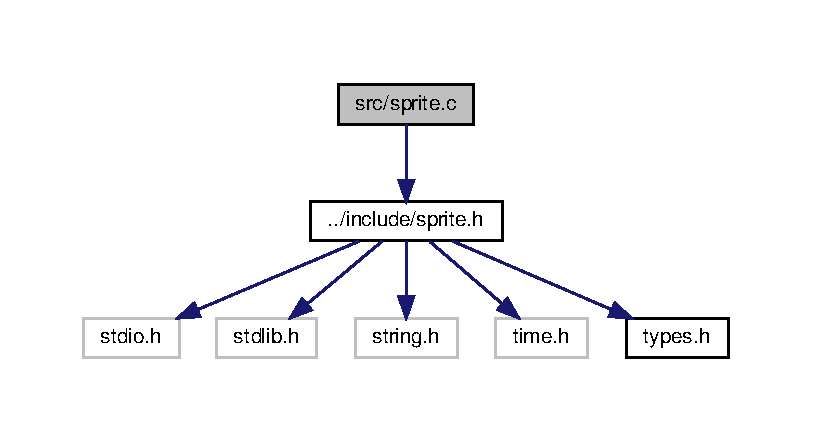
\includegraphics[width=350pt]{sprite_8c__incl}
\end{center}
\end{figure}
\subsection*{Classes}
\begin{DoxyCompactItemize}
\item 
struct \hyperlink{struct__Sprite}{\+\_\+\+Sprite}
\end{DoxyCompactItemize}
\subsection*{Functions}
\begin{DoxyCompactItemize}
\item 
\hyperlink{sprite_8h_a4dac9894071cab0926c0b91f2fe6e9cf}{Sprite} $\ast$ \hyperlink{sprite_8c_a99036d6e48760ddf5034418ecadbb3fe}{sprite\+\_\+create} (\hyperlink{types_8h_a845e604fb28f7e3d97549da3448149d3}{Id} id)
\item 
void \hyperlink{sprite_8c_a23bda5268d3dd5cae3a877ab1a428816}{sprite\+\_\+destroy} (\hyperlink{sprite_8h_a4dac9894071cab0926c0b91f2fe6e9cf}{Sprite} $\ast$sprite)
\item 
\hyperlink{types_8h_a845e604fb28f7e3d97549da3448149d3}{Id} \hyperlink{sprite_8c_a2a730651103936590c0ebab618efa073}{sprite\+\_\+get\+Id} (\hyperlink{sprite_8h_a4dac9894071cab0926c0b91f2fe6e9cf}{Sprite} $\ast$sprite)
\item 
char $\ast$ \hyperlink{sprite_8c_a19119e8b188da7794f6ed137fd0cf9e8}{sprite\+\_\+get\+Data} (\hyperlink{sprite_8h_a4dac9894071cab0926c0b91f2fe6e9cf}{Sprite} $\ast$sprite, int line)
\item 
\hyperlink{types_8h_a32c27cc471df37f4fc818d65de0a56c4}{S\+T\+A\+T\+US} \hyperlink{sprite_8c_a9ff91495bc6194f2dfb1449130f43f2b}{sprite\+\_\+put\+Line} (\hyperlink{sprite_8h_a4dac9894071cab0926c0b91f2fe6e9cf}{Sprite} $\ast$sprite, char $\ast$string, int line)
\item 
void \hyperlink{sprite_8c_ad46d190d28a6771371405d3ebcf63ba8}{sprite\+\_\+print} (\hyperlink{sprite_8h_a4dac9894071cab0926c0b91f2fe6e9cf}{Sprite} $\ast$sprite)
\end{DoxyCompactItemize}


\subsection{Detailed Description}
It declares the sprite module. 

\begin{DoxyAuthor}{Author}
Antonio Solana 
\end{DoxyAuthor}
\begin{DoxyCopyright}{Copyright}
G\+NU Public License 
\end{DoxyCopyright}


\subsection{Function Documentation}
\index{sprite.\+c@{sprite.\+c}!sprite\+\_\+create@{sprite\+\_\+create}}
\index{sprite\+\_\+create@{sprite\+\_\+create}!sprite.\+c@{sprite.\+c}}
\subsubsection[{\texorpdfstring{sprite\+\_\+create(\+Id id)}{sprite_create(Id id)}}]{\setlength{\rightskip}{0pt plus 5cm}{\bf Sprite}$\ast$ sprite\+\_\+create (
\begin{DoxyParamCaption}
\item[{{\bf Id}}]{id}
\end{DoxyParamCaption}
)}\hypertarget{sprite_8c_a99036d6e48760ddf5034418ecadbb3fe}{}\label{sprite_8c_a99036d6e48760ddf5034418ecadbb3fe}
\index{sprite.\+c@{sprite.\+c}!sprite\+\_\+destroy@{sprite\+\_\+destroy}}
\index{sprite\+\_\+destroy@{sprite\+\_\+destroy}!sprite.\+c@{sprite.\+c}}
\subsubsection[{\texorpdfstring{sprite\+\_\+destroy(\+Sprite $\ast$sprite)}{sprite_destroy(Sprite *sprite)}}]{\setlength{\rightskip}{0pt plus 5cm}void sprite\+\_\+destroy (
\begin{DoxyParamCaption}
\item[{{\bf Sprite} $\ast$}]{sprite}
\end{DoxyParamCaption}
)}\hypertarget{sprite_8c_a23bda5268d3dd5cae3a877ab1a428816}{}\label{sprite_8c_a23bda5268d3dd5cae3a877ab1a428816}
\index{sprite.\+c@{sprite.\+c}!sprite\+\_\+get\+Data@{sprite\+\_\+get\+Data}}
\index{sprite\+\_\+get\+Data@{sprite\+\_\+get\+Data}!sprite.\+c@{sprite.\+c}}
\subsubsection[{\texorpdfstring{sprite\+\_\+get\+Data(\+Sprite $\ast$sprite, int line)}{sprite_getData(Sprite *sprite, int line)}}]{\setlength{\rightskip}{0pt plus 5cm}char$\ast$ sprite\+\_\+get\+Data (
\begin{DoxyParamCaption}
\item[{{\bf Sprite} $\ast$}]{sprite, }
\item[{int}]{line}
\end{DoxyParamCaption}
)}\hypertarget{sprite_8c_a19119e8b188da7794f6ed137fd0cf9e8}{}\label{sprite_8c_a19119e8b188da7794f6ed137fd0cf9e8}
\index{sprite.\+c@{sprite.\+c}!sprite\+\_\+get\+Id@{sprite\+\_\+get\+Id}}
\index{sprite\+\_\+get\+Id@{sprite\+\_\+get\+Id}!sprite.\+c@{sprite.\+c}}
\subsubsection[{\texorpdfstring{sprite\+\_\+get\+Id(\+Sprite $\ast$sprite)}{sprite_getId(Sprite *sprite)}}]{\setlength{\rightskip}{0pt plus 5cm}{\bf Id} sprite\+\_\+get\+Id (
\begin{DoxyParamCaption}
\item[{{\bf Sprite} $\ast$}]{sprite}
\end{DoxyParamCaption}
)}\hypertarget{sprite_8c_a2a730651103936590c0ebab618efa073}{}\label{sprite_8c_a2a730651103936590c0ebab618efa073}
\index{sprite.\+c@{sprite.\+c}!sprite\+\_\+print@{sprite\+\_\+print}}
\index{sprite\+\_\+print@{sprite\+\_\+print}!sprite.\+c@{sprite.\+c}}
\subsubsection[{\texorpdfstring{sprite\+\_\+print(\+Sprite $\ast$sprite)}{sprite_print(Sprite *sprite)}}]{\setlength{\rightskip}{0pt plus 5cm}void sprite\+\_\+print (
\begin{DoxyParamCaption}
\item[{{\bf Sprite} $\ast$}]{sprite}
\end{DoxyParamCaption}
)}\hypertarget{sprite_8c_ad46d190d28a6771371405d3ebcf63ba8}{}\label{sprite_8c_ad46d190d28a6771371405d3ebcf63ba8}
\index{sprite.\+c@{sprite.\+c}!sprite\+\_\+put\+Line@{sprite\+\_\+put\+Line}}
\index{sprite\+\_\+put\+Line@{sprite\+\_\+put\+Line}!sprite.\+c@{sprite.\+c}}
\subsubsection[{\texorpdfstring{sprite\+\_\+put\+Line(\+Sprite $\ast$sprite, char $\ast$string, int line)}{sprite_putLine(Sprite *sprite, char *string, int line)}}]{\setlength{\rightskip}{0pt plus 5cm}{\bf S\+T\+A\+T\+US} sprite\+\_\+put\+Line (
\begin{DoxyParamCaption}
\item[{{\bf Sprite} $\ast$}]{sprite, }
\item[{char $\ast$}]{string, }
\item[{int}]{line}
\end{DoxyParamCaption}
)}\hypertarget{sprite_8c_a9ff91495bc6194f2dfb1449130f43f2b}{}\label{sprite_8c_a9ff91495bc6194f2dfb1449130f43f2b}

\hypertarget{sprite_8h}{}\section{include/sprite.h File Reference}
\label{sprite_8h}\index{include/sprite.\+h@{include/sprite.\+h}}


It declares the sprite module.  


{\ttfamily \#include $<$stdio.\+h$>$}\newline
{\ttfamily \#include $<$stdlib.\+h$>$}\newline
{\ttfamily \#include $<$string.\+h$>$}\newline
{\ttfamily \#include $<$time.\+h$>$}\newline
{\ttfamily \#include \char`\"{}types.\+h\char`\"{}}\newline
Include dependency graph for sprite.\+h\+:\nopagebreak
\begin{figure}[H]
\begin{center}
\leavevmode
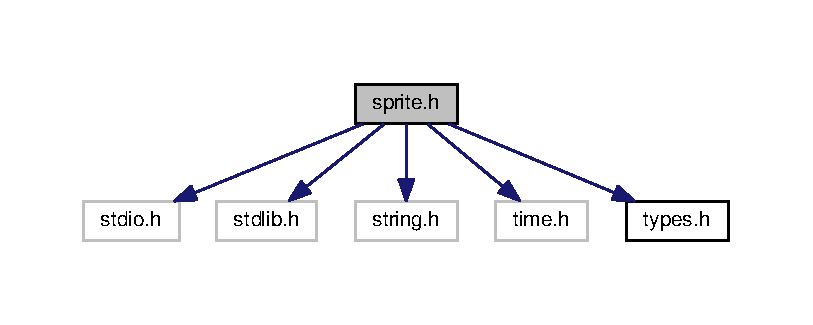
\includegraphics[width=350pt]{sprite_8h__incl}
\end{center}
\end{figure}
This graph shows which files directly or indirectly include this file\+:\nopagebreak
\begin{figure}[H]
\begin{center}
\leavevmode
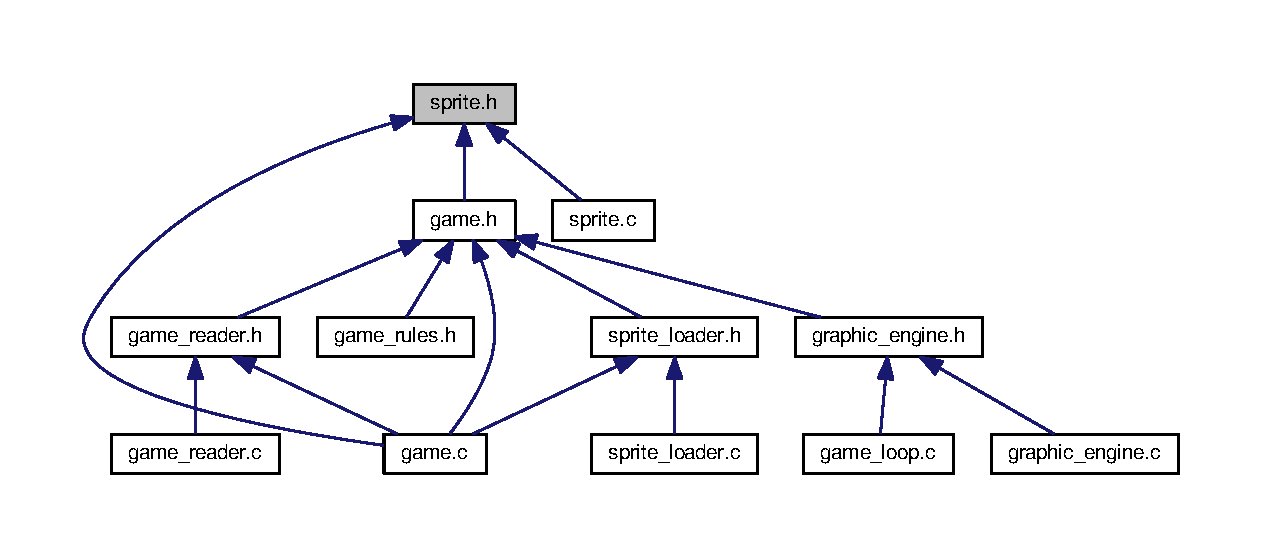
\includegraphics[width=350pt]{sprite_8h__dep__incl}
\end{center}
\end{figure}
\subsection*{Typedefs}
\begin{DoxyCompactItemize}
\item 
\mbox{\Hypertarget{sprite_8h_a4dac9894071cab0926c0b91f2fe6e9cf}\label{sprite_8h_a4dac9894071cab0926c0b91f2fe6e9cf}} 
typedef struct \hyperlink{struct__Sprite}{\+\_\+\+Sprite} {\bfseries Sprite}
\end{DoxyCompactItemize}
\subsection*{Functions}
\begin{DoxyCompactItemize}
\item 
\mbox{\Hypertarget{sprite_8h_a99036d6e48760ddf5034418ecadbb3fe}\label{sprite_8h_a99036d6e48760ddf5034418ecadbb3fe}} 
\hyperlink{struct__Sprite}{Sprite} $\ast$ {\bfseries sprite\+\_\+create} (Id id)
\item 
\mbox{\Hypertarget{sprite_8h_a23bda5268d3dd5cae3a877ab1a428816}\label{sprite_8h_a23bda5268d3dd5cae3a877ab1a428816}} 
void {\bfseries sprite\+\_\+destroy} (\hyperlink{struct__Sprite}{Sprite} $\ast$sprite)
\item 
\mbox{\Hypertarget{sprite_8h_a2a730651103936590c0ebab618efa073}\label{sprite_8h_a2a730651103936590c0ebab618efa073}} 
Id {\bfseries sprite\+\_\+get\+Id} (\hyperlink{struct__Sprite}{Sprite} $\ast$sprite)
\item 
\mbox{\Hypertarget{sprite_8h_a19119e8b188da7794f6ed137fd0cf9e8}\label{sprite_8h_a19119e8b188da7794f6ed137fd0cf9e8}} 
char $\ast$ {\bfseries sprite\+\_\+get\+Data} (\hyperlink{struct__Sprite}{Sprite} $\ast$sprite, int line)
\item 
\mbox{\Hypertarget{sprite_8h_a9ff91495bc6194f2dfb1449130f43f2b}\label{sprite_8h_a9ff91495bc6194f2dfb1449130f43f2b}} 
S\+T\+A\+T\+US {\bfseries sprite\+\_\+put\+Line} (\hyperlink{struct__Sprite}{Sprite} $\ast$sprite, char $\ast$string, int line)
\item 
\mbox{\Hypertarget{sprite_8h_ad46d190d28a6771371405d3ebcf63ba8}\label{sprite_8h_ad46d190d28a6771371405d3ebcf63ba8}} 
void {\bfseries sprite\+\_\+print} (\hyperlink{struct__Sprite}{Sprite} $\ast$sprite)
\end{DoxyCompactItemize}


\subsection{Detailed Description}
It declares the sprite module. 

\begin{DoxyAuthor}{Author}
Antonio Solana 
\end{DoxyAuthor}
\begin{DoxyCopyright}{Copyright}
G\+NU Public License 
\end{DoxyCopyright}

\hypertarget{sprite__loader_8c}{}\section{sprite\+\_\+loader.\+c File Reference}
\label{sprite__loader_8c}\index{sprite\+\_\+loader.\+c@{sprite\+\_\+loader.\+c}}


Reads the sprites from a file.  


{\ttfamily \#include $<$stdio.\+h$>$}\\*
{\ttfamily \#include $<$stdlib.\+h$>$}\\*
{\ttfamily \#include $<$string.\+h$>$}\\*
{\ttfamily \#include \char`\"{}../include/sprite\+\_\+loader.\+h\char`\"{}}\\*
Include dependency graph for sprite\+\_\+loader.\+c\+:\nopagebreak
\begin{figure}[H]
\begin{center}
\leavevmode
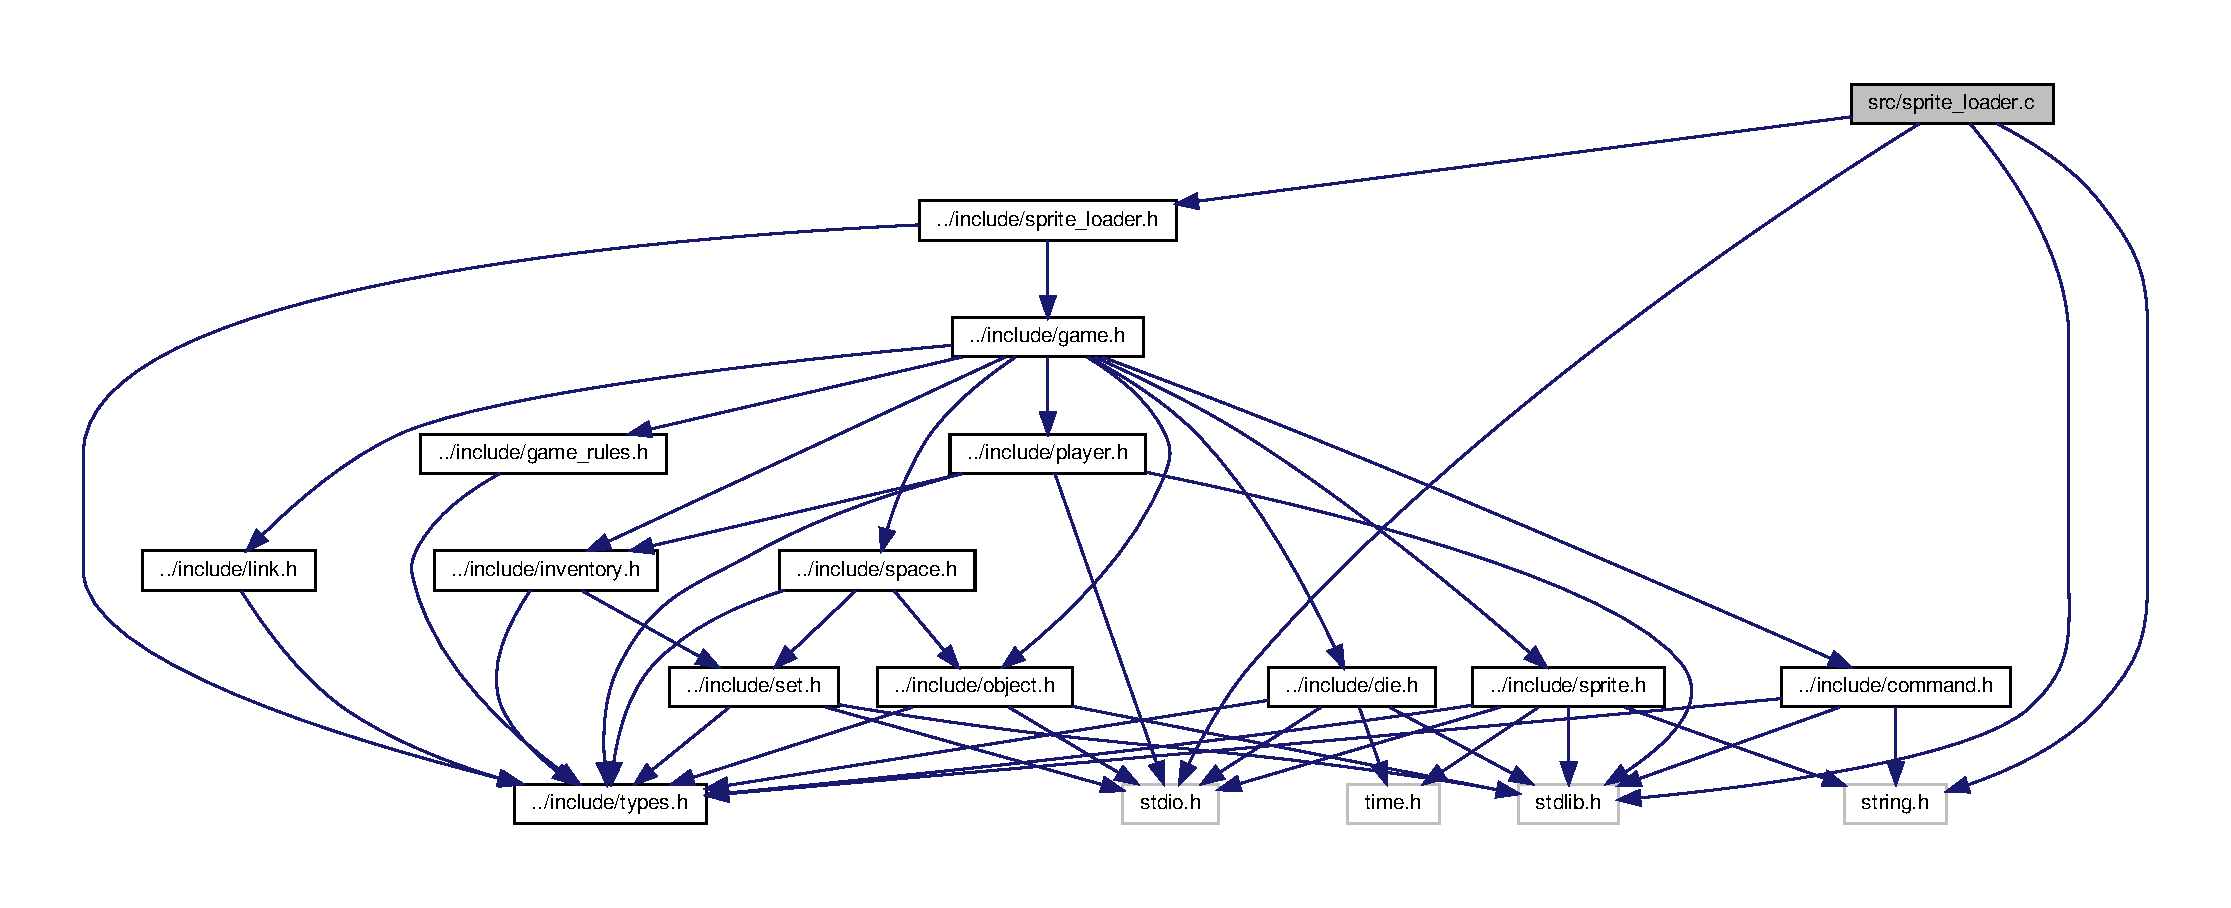
\includegraphics[width=350pt]{sprite__loader_8c__incl}
\end{center}
\end{figure}
\subsection*{Functions}
\begin{DoxyCompactItemize}
\item 
\hyperlink{types_8h_a32c27cc471df37f4fc818d65de0a56c4}{S\+T\+A\+T\+US} \hyperlink{sprite__loader_8c_a95b54bf81580051229d106b362ce5efb}{sprite\+\_\+loader\+\_\+map} (\hyperlink{game_8h_a57156d39c530aec3fba3a9dad8c2dc6a}{Game} $\ast$game, char $\ast$filename)
\end{DoxyCompactItemize}


\subsection{Detailed Description}
Reads the sprites from a file. 

\begin{DoxyAuthor}{Author}
Antonio Solana 
\end{DoxyAuthor}
\begin{DoxyCopyright}{Copyright}
G\+NU Public License 
\end{DoxyCopyright}


\subsection{Function Documentation}
\index{sprite\+\_\+loader.\+c@{sprite\+\_\+loader.\+c}!sprite\+\_\+loader\+\_\+map@{sprite\+\_\+loader\+\_\+map}}
\index{sprite\+\_\+loader\+\_\+map@{sprite\+\_\+loader\+\_\+map}!sprite\+\_\+loader.\+c@{sprite\+\_\+loader.\+c}}
\subsubsection[{\texorpdfstring{sprite\+\_\+loader\+\_\+map(\+Game $\ast$game, char $\ast$filename)}{sprite_loader_map(Game *game, char *filename)}}]{\setlength{\rightskip}{0pt plus 5cm}{\bf S\+T\+A\+T\+US} sprite\+\_\+loader\+\_\+map (
\begin{DoxyParamCaption}
\item[{{\bf Game} $\ast$}]{game, }
\item[{char $\ast$}]{filename}
\end{DoxyParamCaption}
)}\hypertarget{sprite__loader_8c_a95b54bf81580051229d106b362ce5efb}{}\label{sprite__loader_8c_a95b54bf81580051229d106b362ce5efb}

\hypertarget{sprite__loader_8h}{}\section{sprite\+\_\+loader.\+h File Reference}
\label{sprite__loader_8h}\index{sprite\+\_\+loader.\+h@{sprite\+\_\+loader.\+h}}


Reads the sprites from a file.  


{\ttfamily \#include \char`\"{}../include/types.\+h\char`\"{}}\\*
{\ttfamily \#include \char`\"{}../include/game.\+h\char`\"{}}\\*
Include dependency graph for sprite\+\_\+loader.\+h\+:\nopagebreak
\begin{figure}[H]
\begin{center}
\leavevmode
\includegraphics[width=350pt]{sprite__loader_8h__incl}
\end{center}
\end{figure}
This graph shows which files directly or indirectly include this file\+:\nopagebreak
\begin{figure}[H]
\begin{center}
\leavevmode
\includegraphics[width=228pt]{sprite__loader_8h__dep__incl}
\end{center}
\end{figure}
\subsection*{Functions}
\begin{DoxyCompactItemize}
\item 
\hyperlink{types_8h_a32c27cc471df37f4fc818d65de0a56c4}{S\+T\+A\+T\+US} \hyperlink{sprite__loader_8h_a95b54bf81580051229d106b362ce5efb}{sprite\+\_\+loader\+\_\+map} (\hyperlink{game_8h_a57156d39c530aec3fba3a9dad8c2dc6a}{Game} $\ast$game, char $\ast$filename)
\end{DoxyCompactItemize}


\subsection{Detailed Description}
Reads the sprites from a file. 

\begin{DoxyAuthor}{Author}
Antonio Solana 
\end{DoxyAuthor}
\begin{DoxyCopyright}{Copyright}
G\+NU Public License 
\end{DoxyCopyright}


\subsection{Function Documentation}
\index{sprite\+\_\+loader.\+h@{sprite\+\_\+loader.\+h}!sprite\+\_\+loader\+\_\+map@{sprite\+\_\+loader\+\_\+map}}
\index{sprite\+\_\+loader\+\_\+map@{sprite\+\_\+loader\+\_\+map}!sprite\+\_\+loader.\+h@{sprite\+\_\+loader.\+h}}
\subsubsection[{\texorpdfstring{sprite\+\_\+loader\+\_\+map(\+Game $\ast$game, char $\ast$filename)}{sprite_loader_map(Game *game, char *filename)}}]{\setlength{\rightskip}{0pt plus 5cm}{\bf S\+T\+A\+T\+US} sprite\+\_\+loader\+\_\+map (
\begin{DoxyParamCaption}
\item[{{\bf Game} $\ast$}]{game, }
\item[{char $\ast$}]{filename}
\end{DoxyParamCaption}
)}\hypertarget{sprite__loader_8h_a95b54bf81580051229d106b362ce5efb}{}\label{sprite__loader_8h_a95b54bf81580051229d106b362ce5efb}

\hypertarget{test_8h}{}\section{test.\+h File Reference}
\label{test_8h}\index{test.\+h@{test.\+h}}


Test low level functions.  


This graph shows which files directly or indirectly include this file\+:
% FIG 0
\subsection*{Macros}
\begin{DoxyCompactItemize}
\item 
\#define \hyperlink{test_8h_a66290957baed5df3930ada4cb8caccf1}{K\+R\+ED}~\char`\"{}\textbackslash{}x1B\mbox{[}31m\char`\"{}
\item 
\#define \hyperlink{test_8h_ac081c83b067273757f7a2e54a5957d41}{K\+G\+RN}~\char`\"{}\textbackslash{}x1B\mbox{[}32m\char`\"{}
\item 
\#define \hyperlink{test_8h_a897b10d246533c95ba86cb79f92e465a}{K\+Y\+EL}~\char`\"{}\textbackslash{}x1B\mbox{[}33m\char`\"{}
\item 
\#define \hyperlink{test_8h_a32036c94dbb166a3f874b7efc169841f}{K\+C\+YN}~\char`\"{}\textbackslash{}x1B\mbox{[}36m\char`\"{}
\item 
\#define \hyperlink{test_8h_ab702106cf3b3e96750b6845ded4e0299}{R\+E\+S\+ET}~\char`\"{}\textbackslash{}033\mbox{[}0m\char`\"{}
\item 
\#define \hyperlink{test_8h_a6c00863b1d44e38839b1f4b49d04f403}{P\+R\+I\+N\+T\+\_\+\+T\+E\+S\+T\+\_\+\+R\+E\+S\+U\+LT}(x)
\item 
\#define \hyperlink{test_8h_a4a5b9a0026e80b1cfbfbbc3fa700ed31}{P\+R\+I\+N\+T\+\_\+\+P\+A\+S\+S\+E\+D\+\_\+\+P\+E\+R\+C\+E\+N\+T\+A\+GE}~printf(\char`\"{}Tests passed \%d\%\%\textbackslash{}n\char`\"{}, ((\+\_\+\+\_\+test\+\_\+passed $\ast$ 100) / \hyperlink{test_8h_a28f923b76762bf6cab08a34b7c3d87d6}{\+\_\+\+\_\+test\+\_\+counter}))
\end{DoxyCompactItemize}
\subsection*{Variables}
\begin{DoxyCompactItemize}
\item 
static int \hyperlink{test_8h_a28f923b76762bf6cab08a34b7c3d87d6}{\+\_\+\+\_\+test\+\_\+counter} = 0
\item 
static int \hyperlink{test_8h_a1d91487154d9bb3387f6e6318a20336d}{\+\_\+\+\_\+test\+\_\+passed} = 0
\item 
static int \hyperlink{test_8h_a96fad6a57224964f21b17ed22e6c1c4a}{\+\_\+\+\_\+pass} = 0
\end{DoxyCompactItemize}


\subsection{Detailed Description}
Test low level functions. 

\begin{DoxyAuthor}{Author}
Profesores Pprog 
\end{DoxyAuthor}
\begin{DoxyCopyright}{Copyright}
G\+NU Public License 
\end{DoxyCopyright}


\subsection{Macro Definition Documentation}
\index{test.\+h@{test.\+h}!K\+C\+YN@{K\+C\+YN}}
\index{K\+C\+YN@{K\+C\+YN}!test.\+h@{test.\+h}}
\subsubsection[{\texorpdfstring{K\+C\+YN}{KCYN}}]{\setlength{\rightskip}{0pt plus 5cm}\#define K\+C\+YN~\char`\"{}\textbackslash{}x1B\mbox{[}36m\char`\"{}}\hypertarget{test_8h_a32036c94dbb166a3f874b7efc169841f}{}\label{test_8h_a32036c94dbb166a3f874b7efc169841f}
\index{test.\+h@{test.\+h}!K\+G\+RN@{K\+G\+RN}}
\index{K\+G\+RN@{K\+G\+RN}!test.\+h@{test.\+h}}
\subsubsection[{\texorpdfstring{K\+G\+RN}{KGRN}}]{\setlength{\rightskip}{0pt plus 5cm}\#define K\+G\+RN~\char`\"{}\textbackslash{}x1B\mbox{[}32m\char`\"{}}\hypertarget{test_8h_ac081c83b067273757f7a2e54a5957d41}{}\label{test_8h_ac081c83b067273757f7a2e54a5957d41}
\index{test.\+h@{test.\+h}!K\+R\+ED@{K\+R\+ED}}
\index{K\+R\+ED@{K\+R\+ED}!test.\+h@{test.\+h}}
\subsubsection[{\texorpdfstring{K\+R\+ED}{KRED}}]{\setlength{\rightskip}{0pt plus 5cm}\#define K\+R\+ED~\char`\"{}\textbackslash{}x1B\mbox{[}31m\char`\"{}}\hypertarget{test_8h_a66290957baed5df3930ada4cb8caccf1}{}\label{test_8h_a66290957baed5df3930ada4cb8caccf1}
\index{test.\+h@{test.\+h}!K\+Y\+EL@{K\+Y\+EL}}
\index{K\+Y\+EL@{K\+Y\+EL}!test.\+h@{test.\+h}}
\subsubsection[{\texorpdfstring{K\+Y\+EL}{KYEL}}]{\setlength{\rightskip}{0pt plus 5cm}\#define K\+Y\+EL~\char`\"{}\textbackslash{}x1B\mbox{[}33m\char`\"{}}\hypertarget{test_8h_a897b10d246533c95ba86cb79f92e465a}{}\label{test_8h_a897b10d246533c95ba86cb79f92e465a}
\index{test.\+h@{test.\+h}!P\+R\+I\+N\+T\+\_\+\+P\+A\+S\+S\+E\+D\+\_\+\+P\+E\+R\+C\+E\+N\+T\+A\+GE@{P\+R\+I\+N\+T\+\_\+\+P\+A\+S\+S\+E\+D\+\_\+\+P\+E\+R\+C\+E\+N\+T\+A\+GE}}
\index{P\+R\+I\+N\+T\+\_\+\+P\+A\+S\+S\+E\+D\+\_\+\+P\+E\+R\+C\+E\+N\+T\+A\+GE@{P\+R\+I\+N\+T\+\_\+\+P\+A\+S\+S\+E\+D\+\_\+\+P\+E\+R\+C\+E\+N\+T\+A\+GE}!test.\+h@{test.\+h}}
\subsubsection[{\texorpdfstring{P\+R\+I\+N\+T\+\_\+\+P\+A\+S\+S\+E\+D\+\_\+\+P\+E\+R\+C\+E\+N\+T\+A\+GE}{PRINT_PASSED_PERCENTAGE}}]{\setlength{\rightskip}{0pt plus 5cm}\#define P\+R\+I\+N\+T\+\_\+\+P\+A\+S\+S\+E\+D\+\_\+\+P\+E\+R\+C\+E\+N\+T\+A\+GE~printf(\char`\"{}Tests passed \%d\%\%\textbackslash{}n\char`\"{}, ((\+\_\+\+\_\+test\+\_\+passed $\ast$ 100) / {\bf \+\_\+\+\_\+test\+\_\+counter}))}\hypertarget{test_8h_a4a5b9a0026e80b1cfbfbbc3fa700ed31}{}\label{test_8h_a4a5b9a0026e80b1cfbfbbc3fa700ed31}
\index{test.\+h@{test.\+h}!P\+R\+I\+N\+T\+\_\+\+T\+E\+S\+T\+\_\+\+R\+E\+S\+U\+LT@{P\+R\+I\+N\+T\+\_\+\+T\+E\+S\+T\+\_\+\+R\+E\+S\+U\+LT}}
\index{P\+R\+I\+N\+T\+\_\+\+T\+E\+S\+T\+\_\+\+R\+E\+S\+U\+LT@{P\+R\+I\+N\+T\+\_\+\+T\+E\+S\+T\+\_\+\+R\+E\+S\+U\+LT}!test.\+h@{test.\+h}}
\subsubsection[{\texorpdfstring{P\+R\+I\+N\+T\+\_\+\+T\+E\+S\+T\+\_\+\+R\+E\+S\+U\+LT}{PRINT_TEST_RESULT}}]{\setlength{\rightskip}{0pt plus 5cm}\#define P\+R\+I\+N\+T\+\_\+\+T\+E\+S\+T\+\_\+\+R\+E\+S\+U\+LT(
\begin{DoxyParamCaption}
\item[{}]{x}
\end{DoxyParamCaption}
)}\hypertarget{test_8h_a6c00863b1d44e38839b1f4b49d04f403}{}\label{test_8h_a6c00863b1d44e38839b1f4b49d04f403}
{\bfseries Value\+:}
\begin{DoxyCode}
\textcolor{keywordflow}{do}\{\hyperlink{test_8h_a28f923b76762bf6cab08a34b7c3d87d6}{\(\backslash\)}
\hyperlink{test_8h_a28f923b76762bf6cab08a34b7c3d87d6}{    \_\_test\_counter}++;\hyperlink{test_8h_a96fad6a57224964f21b17ed22e6c1c4a}{\(\backslash\)}
\hyperlink{test_8h_a96fad6a57224964f21b17ed22e6c1c4a}{    \_\_pass} = (x);\hyperlink{test_8h_a1d91487154d9bb3387f6e6318a20336d}{\(\backslash\)}
\hyperlink{test_8h_a1d91487154d9bb3387f6e6318a20336d}{    \_\_test\_passed} = (\hyperlink{test_8h_a96fad6a57224964f21b17ed22e6c1c4a}{\_\_pass})? \hyperlink{test_8h_a1d91487154d9bb3387f6e6318a20336d}{\_\_test\_passed} + 1 : 
      \hyperlink{test_8h_a1d91487154d9bb3387f6e6318a20336d}{\_\_test\_passed};\(\backslash\)
    printf(\hyperlink{test_8h_a897b10d246533c95ba86cb79f92e465a}{KYEL} \textcolor{stringliteral}{"%s"} \hyperlink{test_8h_ab702106cf3b3e96750b6845ded4e0299}{RESET} \textcolor{stringliteral}{" line "}  \textcolor{stringliteral}{"%d "} \hyperlink{test_8h_a32036c94dbb166a3f874b7efc169841f}{KCYN} \textcolor{stringliteral}{"%s"} \hyperlink{test_8h_ab702106cf3b3e96750b6845ded4e0299}{RESET} \textcolor{stringliteral}{": %s\(\backslash\)n"}, \(\backslash\)
       \_\_FILE\_\_, \_\_LINE\_\_ , \_\_FUNCTION\_\_, \(\backslash\)
       ((!\hyperlink{test_8h_a96fad6a57224964f21b17ed22e6c1c4a}{\_\_pass}) ? \hyperlink{test_8h_a66290957baed5df3930ada4cb8caccf1}{KRED} \textcolor{stringliteral}{"NOT PASS"} RESET : \hyperlink{test_8h_ac081c83b067273757f7a2e54a5957d41}{KGRN} \textcolor{stringliteral}{"PASS"} RESET));  \(\backslash\)
  \} \textcolor{keywordflow}{while} (0)
\end{DoxyCode}
\index{test.\+h@{test.\+h}!R\+E\+S\+ET@{R\+E\+S\+ET}}
\index{R\+E\+S\+ET@{R\+E\+S\+ET}!test.\+h@{test.\+h}}
\subsubsection[{\texorpdfstring{R\+E\+S\+ET}{RESET}}]{\setlength{\rightskip}{0pt plus 5cm}\#define R\+E\+S\+ET~\char`\"{}\textbackslash{}033\mbox{[}0m\char`\"{}}\hypertarget{test_8h_ab702106cf3b3e96750b6845ded4e0299}{}\label{test_8h_ab702106cf3b3e96750b6845ded4e0299}


\subsection{Variable Documentation}
\index{test.\+h@{test.\+h}!\+\_\+\+\_\+pass@{\+\_\+\+\_\+pass}}
\index{\+\_\+\+\_\+pass@{\+\_\+\+\_\+pass}!test.\+h@{test.\+h}}
\subsubsection[{\texorpdfstring{\+\_\+\+\_\+pass}{__pass}}]{\setlength{\rightskip}{0pt plus 5cm}int \+\_\+\+\_\+pass = 0\hspace{0.3cm}{\ttfamily [static]}}\hypertarget{test_8h_a96fad6a57224964f21b17ed22e6c1c4a}{}\label{test_8h_a96fad6a57224964f21b17ed22e6c1c4a}
\index{test.\+h@{test.\+h}!\+\_\+\+\_\+test\+\_\+counter@{\+\_\+\+\_\+test\+\_\+counter}}
\index{\+\_\+\+\_\+test\+\_\+counter@{\+\_\+\+\_\+test\+\_\+counter}!test.\+h@{test.\+h}}
\subsubsection[{\texorpdfstring{\+\_\+\+\_\+test\+\_\+counter}{__test_counter}}]{\setlength{\rightskip}{0pt plus 5cm}int \+\_\+\+\_\+test\+\_\+counter = 0\hspace{0.3cm}{\ttfamily [static]}}\hypertarget{test_8h_a28f923b76762bf6cab08a34b7c3d87d6}{}\label{test_8h_a28f923b76762bf6cab08a34b7c3d87d6}
\index{test.\+h@{test.\+h}!\+\_\+\+\_\+test\+\_\+passed@{\+\_\+\+\_\+test\+\_\+passed}}
\index{\+\_\+\+\_\+test\+\_\+passed@{\+\_\+\+\_\+test\+\_\+passed}!test.\+h@{test.\+h}}
\subsubsection[{\texorpdfstring{\+\_\+\+\_\+test\+\_\+passed}{__test_passed}}]{\setlength{\rightskip}{0pt plus 5cm}int \+\_\+\+\_\+test\+\_\+passed = 0\hspace{0.3cm}{\ttfamily [static]}}\hypertarget{test_8h_a1d91487154d9bb3387f6e6318a20336d}{}\label{test_8h_a1d91487154d9bb3387f6e6318a20336d}

\hypertarget{types_8h}{}\section{types.\+h File Reference}
\label{types_8h}\index{types.\+h@{types.\+h}}


Global typedefs.  


This graph shows which files directly or indirectly include this file\+:\nopagebreak
\begin{figure}[H]
\begin{center}
\leavevmode
\includegraphics[width=350pt]{types_8h__dep__incl}
\end{center}
\end{figure}
\subsection*{Macros}
\begin{DoxyCompactItemize}
\item 
\#define \hyperlink{types_8h_a92ed8507d1cd2331ad09275c5c4c1c89}{W\+O\+R\+D\+\_\+\+S\+I\+ZE}~1000
\item 
\#define \hyperlink{types_8h_a642e16f35aa1e585c25e405ede76e115}{N\+O\+\_\+\+ID}~-\/1
\item 
\#define \hyperlink{types_8h_a431b1676533a0e1714aff7d6a5542406}{S\+T\+D\+S\+I\+ZE}~1024
\item 
\#define \hyperlink{types_8h_aeb21c7ac080eea985b7701df626d9cf4}{M\+A\+X\+\_\+\+S\+P\+R\+I\+T\+ES}~1000
\item 
\#define \hyperlink{types_8h_ab5187269936538ffb8ccbbe7115ffdbc}{M\+A\+X\+\_\+\+S\+T\+R\+I\+NG}~20
\end{DoxyCompactItemize}
\subsection*{Typedefs}
\begin{DoxyCompactItemize}
\item 
typedef long \hyperlink{types_8h_a845e604fb28f7e3d97549da3448149d3}{Id}
\end{DoxyCompactItemize}
\subsection*{Enumerations}
\begin{DoxyCompactItemize}
\item 
enum \hyperlink{types_8h_a3e5b8192e7d9ffaf3542f1210aec18dd}{B\+O\+OL} \{ \hyperlink{types_8h_a3e5b8192e7d9ffaf3542f1210aec18ddaa1e095cc966dbecf6a0d8aad75348d1a}{F\+A\+L\+SE}, 
\hyperlink{types_8h_a3e5b8192e7d9ffaf3542f1210aec18ddaa82764c3079aea4e60c80e45befbb839}{T\+R\+UE}
 \}
\item 
enum \hyperlink{types_8h_a32c27cc471df37f4fc818d65de0a56c4}{S\+T\+A\+T\+US} \{ \hyperlink{types_8h_a32c27cc471df37f4fc818d65de0a56c4a2fd6f336d08340583bd620a7f5694c90}{E\+R\+R\+OR}, 
\hyperlink{types_8h_a32c27cc471df37f4fc818d65de0a56c4a2bc49ec37d6a5715dd23e85f1ff5bb59}{OK}
 \}
\item 
enum \hyperlink{types_8h_aa268a41a13430b18e933ed40207178d0}{D\+I\+R\+E\+C\+T\+I\+ON} \{ \hyperlink{types_8h_aa268a41a13430b18e933ed40207178d0ad0611de6f28d4a9c9eac959f5344698e}{N\+O\+R\+TH}, 
\hyperlink{types_8h_aa268a41a13430b18e933ed40207178d0ab5b3793b961949c817c7c0d99c05dad7}{E\+A\+ST}, 
\hyperlink{types_8h_aa268a41a13430b18e933ed40207178d0a8ef5c0bce69283a9986011a63eea8a6b}{S\+O\+U\+TH}, 
\hyperlink{types_8h_aa268a41a13430b18e933ed40207178d0ae9449e8683a8199dad36b07a63b2f523}{W\+E\+ST}
 \}
\item 
enum \hyperlink{types_8h_aa60f669816b146d6373c62d9625e52ad}{Link\+Status} \{ \hyperlink{types_8h_aa60f669816b146d6373c62d9625e52ada45c1c97bdcce420fc01045ee101a0cf2}{O\+P\+E\+N\+ED}, 
\hyperlink{types_8h_aa60f669816b146d6373c62d9625e52ada929f0327e17604ce9713b2a6117bd603}{C\+L\+O\+S\+ED}, 
\hyperlink{types_8h_aa60f669816b146d6373c62d9625e52adaba43fad8ee5185f12ea31f7dcb843709}{N\+O\+\_\+\+L\+I\+NK}
 \}
\end{DoxyCompactItemize}


\subsection{Detailed Description}
Global typedefs. 

\begin{DoxyAuthor}{Author}
N\+O\+N\+A\+ME 
\end{DoxyAuthor}
\begin{DoxyCopyright}{Copyright}
G\+NU Public License 
\end{DoxyCopyright}


\subsection{Macro Definition Documentation}
\index{types.\+h@{types.\+h}!M\+A\+X\+\_\+\+S\+P\+R\+I\+T\+ES@{M\+A\+X\+\_\+\+S\+P\+R\+I\+T\+ES}}
\index{M\+A\+X\+\_\+\+S\+P\+R\+I\+T\+ES@{M\+A\+X\+\_\+\+S\+P\+R\+I\+T\+ES}!types.\+h@{types.\+h}}
\subsubsection[{\texorpdfstring{M\+A\+X\+\_\+\+S\+P\+R\+I\+T\+ES}{MAX_SPRITES}}]{\setlength{\rightskip}{0pt plus 5cm}\#define M\+A\+X\+\_\+\+S\+P\+R\+I\+T\+ES~1000}\hypertarget{types_8h_aeb21c7ac080eea985b7701df626d9cf4}{}\label{types_8h_aeb21c7ac080eea985b7701df626d9cf4}
\index{types.\+h@{types.\+h}!M\+A\+X\+\_\+\+S\+T\+R\+I\+NG@{M\+A\+X\+\_\+\+S\+T\+R\+I\+NG}}
\index{M\+A\+X\+\_\+\+S\+T\+R\+I\+NG@{M\+A\+X\+\_\+\+S\+T\+R\+I\+NG}!types.\+h@{types.\+h}}
\subsubsection[{\texorpdfstring{M\+A\+X\+\_\+\+S\+T\+R\+I\+NG}{MAX_STRING}}]{\setlength{\rightskip}{0pt plus 5cm}\#define M\+A\+X\+\_\+\+S\+T\+R\+I\+NG~20}\hypertarget{types_8h_ab5187269936538ffb8ccbbe7115ffdbc}{}\label{types_8h_ab5187269936538ffb8ccbbe7115ffdbc}
\index{types.\+h@{types.\+h}!N\+O\+\_\+\+ID@{N\+O\+\_\+\+ID}}
\index{N\+O\+\_\+\+ID@{N\+O\+\_\+\+ID}!types.\+h@{types.\+h}}
\subsubsection[{\texorpdfstring{N\+O\+\_\+\+ID}{NO_ID}}]{\setlength{\rightskip}{0pt plus 5cm}\#define N\+O\+\_\+\+ID~-\/1}\hypertarget{types_8h_a642e16f35aa1e585c25e405ede76e115}{}\label{types_8h_a642e16f35aa1e585c25e405ede76e115}
\index{types.\+h@{types.\+h}!S\+T\+D\+S\+I\+ZE@{S\+T\+D\+S\+I\+ZE}}
\index{S\+T\+D\+S\+I\+ZE@{S\+T\+D\+S\+I\+ZE}!types.\+h@{types.\+h}}
\subsubsection[{\texorpdfstring{S\+T\+D\+S\+I\+ZE}{STDSIZE}}]{\setlength{\rightskip}{0pt plus 5cm}\#define S\+T\+D\+S\+I\+ZE~1024}\hypertarget{types_8h_a431b1676533a0e1714aff7d6a5542406}{}\label{types_8h_a431b1676533a0e1714aff7d6a5542406}
\index{types.\+h@{types.\+h}!W\+O\+R\+D\+\_\+\+S\+I\+ZE@{W\+O\+R\+D\+\_\+\+S\+I\+ZE}}
\index{W\+O\+R\+D\+\_\+\+S\+I\+ZE@{W\+O\+R\+D\+\_\+\+S\+I\+ZE}!types.\+h@{types.\+h}}
\subsubsection[{\texorpdfstring{W\+O\+R\+D\+\_\+\+S\+I\+ZE}{WORD_SIZE}}]{\setlength{\rightskip}{0pt plus 5cm}\#define W\+O\+R\+D\+\_\+\+S\+I\+ZE~1000}\hypertarget{types_8h_a92ed8507d1cd2331ad09275c5c4c1c89}{}\label{types_8h_a92ed8507d1cd2331ad09275c5c4c1c89}


\subsection{Typedef Documentation}
\index{types.\+h@{types.\+h}!Id@{Id}}
\index{Id@{Id}!types.\+h@{types.\+h}}
\subsubsection[{\texorpdfstring{Id}{Id}}]{\setlength{\rightskip}{0pt plus 5cm}typedef long {\bf Id}}\hypertarget{types_8h_a845e604fb28f7e3d97549da3448149d3}{}\label{types_8h_a845e604fb28f7e3d97549da3448149d3}


\subsection{Enumeration Type Documentation}
\index{types.\+h@{types.\+h}!B\+O\+OL@{B\+O\+OL}}
\index{B\+O\+OL@{B\+O\+OL}!types.\+h@{types.\+h}}
\subsubsection[{\texorpdfstring{B\+O\+OL}{BOOL}}]{\setlength{\rightskip}{0pt plus 5cm}enum {\bf B\+O\+OL}}\hypertarget{types_8h_a3e5b8192e7d9ffaf3542f1210aec18dd}{}\label{types_8h_a3e5b8192e7d9ffaf3542f1210aec18dd}
\begin{Desc}
\item[Enumerator]\par
\begin{description}
\index{F\+A\+L\+SE@{F\+A\+L\+SE}!types.\+h@{types.\+h}}\index{types.\+h@{types.\+h}!F\+A\+L\+SE@{F\+A\+L\+SE}}\item[{\em 
F\+A\+L\+SE\hypertarget{types_8h_a3e5b8192e7d9ffaf3542f1210aec18ddaa1e095cc966dbecf6a0d8aad75348d1a}{}\label{types_8h_a3e5b8192e7d9ffaf3542f1210aec18ddaa1e095cc966dbecf6a0d8aad75348d1a}
}]\index{T\+R\+UE@{T\+R\+UE}!types.\+h@{types.\+h}}\index{types.\+h@{types.\+h}!T\+R\+UE@{T\+R\+UE}}\item[{\em 
T\+R\+UE\hypertarget{types_8h_a3e5b8192e7d9ffaf3542f1210aec18ddaa82764c3079aea4e60c80e45befbb839}{}\label{types_8h_a3e5b8192e7d9ffaf3542f1210aec18ddaa82764c3079aea4e60c80e45befbb839}
}]\end{description}
\end{Desc}
\index{types.\+h@{types.\+h}!D\+I\+R\+E\+C\+T\+I\+ON@{D\+I\+R\+E\+C\+T\+I\+ON}}
\index{D\+I\+R\+E\+C\+T\+I\+ON@{D\+I\+R\+E\+C\+T\+I\+ON}!types.\+h@{types.\+h}}
\subsubsection[{\texorpdfstring{D\+I\+R\+E\+C\+T\+I\+ON}{DIRECTION}}]{\setlength{\rightskip}{0pt plus 5cm}enum {\bf D\+I\+R\+E\+C\+T\+I\+ON}}\hypertarget{types_8h_aa268a41a13430b18e933ed40207178d0}{}\label{types_8h_aa268a41a13430b18e933ed40207178d0}
\begin{Desc}
\item[Enumerator]\par
\begin{description}
\index{N\+O\+R\+TH@{N\+O\+R\+TH}!types.\+h@{types.\+h}}\index{types.\+h@{types.\+h}!N\+O\+R\+TH@{N\+O\+R\+TH}}\item[{\em 
N\+O\+R\+TH\hypertarget{types_8h_aa268a41a13430b18e933ed40207178d0ad0611de6f28d4a9c9eac959f5344698e}{}\label{types_8h_aa268a41a13430b18e933ed40207178d0ad0611de6f28d4a9c9eac959f5344698e}
}]\index{E\+A\+ST@{E\+A\+ST}!types.\+h@{types.\+h}}\index{types.\+h@{types.\+h}!E\+A\+ST@{E\+A\+ST}}\item[{\em 
E\+A\+ST\hypertarget{types_8h_aa268a41a13430b18e933ed40207178d0ab5b3793b961949c817c7c0d99c05dad7}{}\label{types_8h_aa268a41a13430b18e933ed40207178d0ab5b3793b961949c817c7c0d99c05dad7}
}]\index{S\+O\+U\+TH@{S\+O\+U\+TH}!types.\+h@{types.\+h}}\index{types.\+h@{types.\+h}!S\+O\+U\+TH@{S\+O\+U\+TH}}\item[{\em 
S\+O\+U\+TH\hypertarget{types_8h_aa268a41a13430b18e933ed40207178d0a8ef5c0bce69283a9986011a63eea8a6b}{}\label{types_8h_aa268a41a13430b18e933ed40207178d0a8ef5c0bce69283a9986011a63eea8a6b}
}]\index{W\+E\+ST@{W\+E\+ST}!types.\+h@{types.\+h}}\index{types.\+h@{types.\+h}!W\+E\+ST@{W\+E\+ST}}\item[{\em 
W\+E\+ST\hypertarget{types_8h_aa268a41a13430b18e933ed40207178d0ae9449e8683a8199dad36b07a63b2f523}{}\label{types_8h_aa268a41a13430b18e933ed40207178d0ae9449e8683a8199dad36b07a63b2f523}
}]\end{description}
\end{Desc}
\index{types.\+h@{types.\+h}!Link\+Status@{Link\+Status}}
\index{Link\+Status@{Link\+Status}!types.\+h@{types.\+h}}
\subsubsection[{\texorpdfstring{Link\+Status}{LinkStatus}}]{\setlength{\rightskip}{0pt plus 5cm}enum {\bf Link\+Status}}\hypertarget{types_8h_aa60f669816b146d6373c62d9625e52ad}{}\label{types_8h_aa60f669816b146d6373c62d9625e52ad}
\begin{Desc}
\item[Enumerator]\par
\begin{description}
\index{O\+P\+E\+N\+ED@{O\+P\+E\+N\+ED}!types.\+h@{types.\+h}}\index{types.\+h@{types.\+h}!O\+P\+E\+N\+ED@{O\+P\+E\+N\+ED}}\item[{\em 
O\+P\+E\+N\+ED\hypertarget{types_8h_aa60f669816b146d6373c62d9625e52ada45c1c97bdcce420fc01045ee101a0cf2}{}\label{types_8h_aa60f669816b146d6373c62d9625e52ada45c1c97bdcce420fc01045ee101a0cf2}
}]\index{C\+L\+O\+S\+ED@{C\+L\+O\+S\+ED}!types.\+h@{types.\+h}}\index{types.\+h@{types.\+h}!C\+L\+O\+S\+ED@{C\+L\+O\+S\+ED}}\item[{\em 
C\+L\+O\+S\+ED\hypertarget{types_8h_aa60f669816b146d6373c62d9625e52ada929f0327e17604ce9713b2a6117bd603}{}\label{types_8h_aa60f669816b146d6373c62d9625e52ada929f0327e17604ce9713b2a6117bd603}
}]\index{N\+O\+\_\+\+L\+I\+NK@{N\+O\+\_\+\+L\+I\+NK}!types.\+h@{types.\+h}}\index{types.\+h@{types.\+h}!N\+O\+\_\+\+L\+I\+NK@{N\+O\+\_\+\+L\+I\+NK}}\item[{\em 
N\+O\+\_\+\+L\+I\+NK\hypertarget{types_8h_aa60f669816b146d6373c62d9625e52adaba43fad8ee5185f12ea31f7dcb843709}{}\label{types_8h_aa60f669816b146d6373c62d9625e52adaba43fad8ee5185f12ea31f7dcb843709}
}]\end{description}
\end{Desc}
\index{types.\+h@{types.\+h}!S\+T\+A\+T\+US@{S\+T\+A\+T\+US}}
\index{S\+T\+A\+T\+US@{S\+T\+A\+T\+US}!types.\+h@{types.\+h}}
\subsubsection[{\texorpdfstring{S\+T\+A\+T\+US}{STATUS}}]{\setlength{\rightskip}{0pt plus 5cm}enum {\bf S\+T\+A\+T\+US}}\hypertarget{types_8h_a32c27cc471df37f4fc818d65de0a56c4}{}\label{types_8h_a32c27cc471df37f4fc818d65de0a56c4}
\begin{Desc}
\item[Enumerator]\par
\begin{description}
\index{E\+R\+R\+OR@{E\+R\+R\+OR}!types.\+h@{types.\+h}}\index{types.\+h@{types.\+h}!E\+R\+R\+OR@{E\+R\+R\+OR}}\item[{\em 
E\+R\+R\+OR\hypertarget{types_8h_a32c27cc471df37f4fc818d65de0a56c4a2fd6f336d08340583bd620a7f5694c90}{}\label{types_8h_a32c27cc471df37f4fc818d65de0a56c4a2fd6f336d08340583bd620a7f5694c90}
}]\index{OK@{OK}!types.\+h@{types.\+h}}\index{types.\+h@{types.\+h}!OK@{OK}}\item[{\em 
OK\hypertarget{types_8h_a32c27cc471df37f4fc818d65de0a56c4a2bc49ec37d6a5715dd23e85f1ff5bb59}{}\label{types_8h_a32c27cc471df37f4fc818d65de0a56c4a2bc49ec37d6a5715dd23e85f1ff5bb59}
}]\end{description}
\end{Desc}

%--- End generated contents ---

% Index
\backmatter
\newpage
\phantomsection
\clearemptydoublepage
\addcontentsline{toc}{chapter}{Index}
\printindex

\end{document}
